\documentclass[11pt,a4paper,openany]{report}
\usepackage[T1]{fontenc}
\usepackage[utf8]{inputenc}
\usepackage{lmodern}
\usepackage[margin=23mm]{geometry}
\usepackage{amsmath,amssymb,amsthm,mathtools}
\usepackage{longtable,booktabs,array,calc}
\newcounter{none}
\usepackage{graphicx,xcolor,tikz}
\usepackage{microtype}
\usepackage[unicode,breaklinks,colorlinks,linkcolor=blue!45!black,urlcolor=blue!45!black]{hyperref}
\urlstyle{same}
\providecommand{\tightlist}{\setlength{\itemsep}{0pt}\setlength{\parskip}{0pt}}
\providecommand{\passthrough}[1]{#1}
\providecommand{\NL}{\operatorname{NL}}
\providecommand{\colim}{\operatorname*{colim}}
\setlength{\parindent}{0pt}
\setlength{\parskip}{.4em}
\setlength{\emergencystretch}{3em}
\setcounter{tocdepth}{1}
\setcounter{secnumdepth}{0}
\renewcommand{\chaptername}{Lesson}
\DeclareUnicodeCharacter{03BB}{\ensuremath{\lambda}}
\DeclareUnicodeCharacter{0393}{\ensuremath{\Gamma}}
\DeclareUnicodeCharacter{2192}{\ensuremath{\rightarrow}}
\DeclareUnicodeCharacter{2011}{-}
\DeclareUnicodeCharacter{202F}{\,}
\DeclareUnicodeCharacter{2212}{\ensuremath{-}}
\DeclareUnicodeCharacter{03B1}{\ensuremath{\alpha}}
\DeclareUnicodeCharacter{03B2}{\ensuremath{\beta}}
\DeclareUnicodeCharacter{03BC}{\ensuremath{\mu}}
\DeclareUnicodeCharacter{03A6}{\ensuremath{\Phi}}
\DeclareUnicodeCharacter{2260}{\ensuremath{\ne}}
\DeclareUnicodeCharacter{00D7}{\ensuremath{\times}}
\DeclareUnicodeCharacter{2082}{\ensuremath{_2}}
\DeclareUnicodeCharacter{2228}{\ensuremath{\vee}}
\DeclareUnicodeCharacter{2032}{\ensuremath{^{\prime}}}
\DeclareUnicodeCharacter{220E}{\ensuremath{\square}}
\title{Reductive group schemes}
\author{GPT-6.1 Sol (OpenAI)\\Codex, Ultra setting}
\date{October 2026}
\begin{document}
\hypersetup{pageanchor=false}
\maketitle
\pagenumbering{roman}
\hypersetup{pageanchor=true}
\noindent Written and self-checked by the writing AI. No human or independent review is claimed.
Original contributions are dedicated under CC0 1.0. Attributed Stacks adaptations retain
their GNU Free Documentation License obligations, as recorded for each component.
The cumulative collection includes the complete version 1.2 licence below.
\par\medskip
\noindent Online course: \url{https://kokunoyumeto.github.io/open-math-courses/courses/AG-RG/}.
\begingroup\small\tableofcontents\endgroup
\clearpage
\pagenumbering{arabic}
\chapter*{Algebra and sheaf cohomology before reductive groups}\addcontentsline{toc}{chapter}{Algebra and sheaf cohomology before reductive groups}\label{AG-RG-S01-algebra-and-sheaf-cohomology-before-reductive-groups}

\emph{Written and self-checked by GPT-6.1 Sol (OpenAI), Codex, Ultra effort, October 2026. Draft. Original explanations are CC0. The explicitly identified programme proof reproduced in Section 6 retains its existing component terms.}

This supporting lesson supplies the algebra, affine sheaf correspondence, injective resolutions and finite-cover comparisons used by the reductive-group lessons. Rings are commutative with identity. A scheme means a locally ringed space covered by spectra of rings, with their localization structure sheaves; a quasi-coherent module means a sheaf locally obtained from a module. These are definitions, not vanishing or descent theorems. No Noetherian or finite-generation assumption is implicit.

\section{1. The algebra of localization}\label{AG-RG-S01-the-algebra-of-localization}

For a multiplicative subset \(S\) of a ring \(A\), define \(S^{-1}M\) by pairs \((m,s)\) with \((m,s)=(n,t)\) when \(u(tm-sn)=0\) for some \(u\in S\). Addition and scalar multiplication have the usual common-denominator formulas. The map \(S^{-1}A\otimes_A M\to S^{-1}M\), \((a/s)\otimes m\mapsto am/s\), has inverse \(m/s\mapsto (1/s)\otimes m\); the defining equivalence makes both maps well defined.

\textbf{Lemma 1.1.} Localization is exact. Filtered colimits of modules are exact. A module is zero if all its localizations at prime ideals are zero.

\textbf{Proof.} A fraction \(m/s\) maps to zero precisely when some \(u\in S\) kills the image of \(m\). Replace \(m/s\) by \(um/(us)\) to lift it from the kernel. An element of the localization of an injected module maps to zero only when the same multiplier kills it in that module. Surjectivity is obtained by lifting the numerator. This proves exactness. In a filtered colimit every element is represented at one stage, and an equality between finitely many representatives holds at a common later stage. Applying these two facts to kernels and surjections proves exactness of filtered colimits. If \(m\ne0\), its annihilator is a proper ideal. It lies in a maximal ideal \(\mathfrak m\), by Zorn's lemma applied to proper ideals; then \(m/1\ne0\) in \(M_{\mathfrak m}\), since an element outside \(\mathfrak m\) cannot annihilate \(m\). This proves the last assertion. \(\square\)

A module is \textbf{flat} when tensoring with it preserves injections, and consequently short exact sequences, since tensor is right exact by its presentation as generators and bilinear relations. Exactness of localization proves that \(S^{-1}A\) is flat. An exact functor preserves the kernel and image of a differential, so flat tensor commutes with the cohomology of every complex. Tensor commutes with finite sums and products because both are the same finite direct sum.

\textbf{Lemma 1.2 (Nakayama and local finite projectivity).} If \(M\) is finitely generated and \(M=JM\), then some \(a\in J\) satisfies \((1-a)M=0\). If \(J\) is contained in the Jacobson radical, \(M=0\). A finitely presented flat module over a local ring is finite free; over any ring it is locally finite free.

\textbf{Proof.} Write generators \(m_i\) as \(m_i=\sum_j a_{ij}m_j\), with \(a_{ij}\in J\). Multiply the matrix equation \((I-(a_{ij}))m=0\) by its adjugate. Its determinant is \(1-a\) for \(a\in J\), proving the first assertion. Elements \(1-a\) are units when \(J\) lies in every maximal ideal: otherwise a maximal ideal containing \(1-a\) would contain one. This proves the second assertion.

Over a local ring \((A,\mathfrak m)\) lift a basis of \(M/\mathfrak m M\) to obtain a surjection \(A^r\to M\) by Nakayama. Its kernel \(K\) is finite, by finite presentation. Flatness of \(M\) makes \(0\to K\otimes A/\mathfrak m\to (A/\mathfrak m)^r\to M/\mathfrak mM\to0\) exact: tensor the presentation and use preservation of kernels in a free presentation, equivalently resolve the last module by free modules and use exact flat tensor. The last map is an isomorphism, so \(K/\mathfrak mK=0\). Nakayama gives \(K=0\). For a prime of a general ring the same argument applies after localization. The resulting basis and its inverse use finitely many elements, relations and denominators; clearing their denominators gives a principal neighbourhood on which the presentation is free. This proves local finite freeness. \(\square\)

Here the elementary tensor-kernel assertion can be established without derived notation: if \(0\to K\to F\to M\to0\) with \(F\) free and \(M\) flat, and \(N\) is presented as \(F_1\to F_0\to N\to0\) with the \(F_i\) free, lift a proposed kernel element to \(K\otimes F_0\). Its image in \(F\otimes F_0\) comes from \(F\otimes F_1\). Its image in \(M\otimes F_1\) maps to zero in \(M\otimes F_0\); flatness identifies this kernel with the image of \(M\otimes\ker(F_1\to F_0)\). Lift those elements to \(F\), subtract them, and then lift the remaining element from \(K\otimes F_1\). The proposed element was zero in \(K\otimes N\).

\textbf{Lemma 1.3 (the Noetherian inputs).} A finitely generated algebra over a Noetherian ring is Noetherian. Submodules of finite modules over a Noetherian ring are finite.

\textbf{Proof.} For an ideal \(I\subset A[x]\), the leading coefficients of elements of degree at most \(d\) form an ascending sequence of ideals \(L_d\) of \(A\). This sequence stabilizes, and every \(L_d\) before stabilization is finitely generated. Choose polynomials of the corresponding degrees whose leading coefficients generate these finitely many ideals. Given any polynomial in \(I\), subtract suitable multiples of these chosen polynomials to cancel its highest term; for degrees above stabilization multiply the stabilized generators by powers of \(x\). Induction on degree expresses it in the ideal of the finitely many chosen polynomials. Thus \(A[x]\) is Noetherian. Iterate and take a quotient. For a submodule of \(A^r\), projection to the last coordinate has image an ideal, and its kernel is a submodule of \(A^{r-1}\). Induction and lifting ideal generators make the submodule finite. A finite module is a quotient of some \(A^r\); apply the same statement to the inverse image of its submodule. \(\square\)

\phantomsection\label{AG-RG-S01-tor-calculus}

\textbf{Lemma 1.A (Tor for arbitrary modules).} Let \(R\) be any commutative ring and \(M,N\) any modules. Choose a free resolution \(P_\bullet\to M\) by taking a free surjection onto the module and then onto each successive kernel, and define \(\operatorname{Tor}_i^R(M,N)=H_i(P_\bullet\otimes_R N)\). This definition is independent of the resolution, naturally symmetric in \(M,N\), and has the natural long exact sequence of a short exact sequence in either variable.

\textbf{Proof.}

For completeness, the resolution facts used here have the following algebraic proof. Given free resolutions \(P_\bullet\to M\) and \(P'_\bullet\to M'\) and a map \(M\to M'\), lift it to \(P_0\to P'_0\). If maps have been chosen through degree \(i-1\), the image of \(d(P_i)\) lies in the cycles of \(P'_{i-1}\), which are the image of \(P'_i\); freeness of \(P_i\) therefore supplies the next lift. Two such lifts are chain homotopic: after the homotopy has been chosen below degree \(i\), their degree-\(i\) difference minus the already prescribed homotopy term maps to zero under the next differential, and freeness lifts it to \(P'_{i+1}\). The same induction starts at degree zero because both lifts induce the same map on the augmentation. Tensoring preserves the homotopy identity. Thus induced homology maps are independent of the lifts, preserve compositions, and comparison maps between two resolutions of the same module are inverse on homology.

Let \(Q_\bullet\to N\) be another free resolution and form the first-quadrant double complex \(D_{p,q}=P_p\otimes_R Q_q\), with total differential \(d_P\otimes1+(-1)^p1\otimes d_Q\). Augmentation gives maps from its total complex to \(P_\bullet\otimes_R N\) and to \(M\otimes_R Q_\bullet\). Each is a homology isomorphism. Indeed, filter by the degree in the unaugmented direction. In the other direction each augmented row or column is exact because its fixed factor is free. To check the resulting homology assertion directly, start with the outermost nonzero component of a cycle in the augmented kernel and use this exactness to subtract a total boundary that removes that component; proceed to the next component. A chain in any fixed total degree has only finitely many components, so this process terminates. The same process applied to boundaries proves injectivity. The comparison maps just constructed make these two augmentation isomorphisms natural. Interchanging the two resolutions, with the sign \((-1)^{pq}\) on \(P_p\otimes_RQ_q\), consequently gives \[
\operatorname{Tor}_i^R(M,N)\simeq\operatorname{Tor}_i^R(N,M).
\] In particular Tor can be computed using a free resolution of either variable; a projective resolution works as well, since projectives are summands of free modules and the same lifting and exactness arguments apply.

For \(0\to N'\to N\to N''\to0\), tensoring in each degree with the free module \(P_i\) gives a short exact sequence of complexes. If a cycle in the quotient complex is lifted to the middle complex, its differential lies in the subcomplex and is a cycle there. Its homology class is independent of the lift and of the cycle representative: changing either changes that differential by a boundary. This defines the connecting map. The equations saying that a class maps to zero say precisely that one can subtract a boundary and lift it to the preceding complex; they prove exactness at each position. The construction commutes with maps of short exact sequences and gives \[
\cdots\longrightarrow\operatorname{Tor}_i^R(M,N')
\longrightarrow\operatorname{Tor}_i^R(M,N)
\longrightarrow\operatorname{Tor}_i^R(M,N'')
\longrightarrow\operatorname{Tor}_{i-1}^R(M,N')\longrightarrow\cdots,
\] ending in \[
\operatorname{Tor}_1^R(M,N'')\longrightarrow M\otimes_RN'
\longrightarrow M\otimes_RN\longrightarrow M\otimes_RN''\longrightarrow0.
\] Balance gives the corresponding sequence in the first variable. These arguments require neither Noetherianity nor finite generation. \(\square\)

\section{2. Modules on an affine scheme}\label{AG-RG-S01-modules-on-an-affine-scheme}

\textbf{Lemma 2.1 (the principal-cover calculation).} If \(f_1,\ldots,f_r\) generate the unit ideal in \(A\), the augmented alternating complex

\[
0\longrightarrow M\longrightarrow\prod_i M_{f_i}
\longrightarrow\prod_{i<j}M_{f_if_j}\longrightarrow\cdots
\]

is exact for every \(A\)-module \(M\).

\textbf{Proof.} Localize at \(f_a\). Regard an ordered cochain as alternating, with repeated indices zero. Inserting \(a\) as its first index defines a homotopy \(h\) lowering degree, including projection to \(M_{f_a}\) in degree zero. Every extra denominator \(f_a\) is already a unit. Expanding the alternating differential gives \(dh+hd=1\). The localized augmented complex is contractible. Localization commutes with its finite products and its cohomology by Lemma 1.1. If an element of a cohomology module vanishes at every \(f_a\), powers \(f_a^{n_a}\) all kill it. These powers generate one: an ideal they generate, if proper, lies in a maximal ideal containing every \(f_a\), contradicting the unit-ideal hypothesis. A linear combination equal to one kills the element. Thus the original cohomology is zero. \(\square\)

The opens \(D(f)\) form a basis of \(\operatorname{Spec}A\). A collection of them covers precisely when its elements generate one: a proper generated ideal lies in a maximal ideal, and otherwise a finite linear combination already equals one. This also proves quasi-compactness and existence of finite principal refinements of arbitrary open covers.

Define \(\widetilde M\) on this basis by \(\widetilde M(D(f))=M_f\). The first three terms of Lemma 2.1 give the sheaf gluing axiom on every finite principal cover. An arbitrary cover has a finite principal refinement, so these basis values extend to a sheaf, uniquely. Its stalk at \(\mathfrak p\) is \(M_{\mathfrak p}\). Exactness of localization therefore makes \(M\mapsto\widetilde M\) exact.

\textbf{Proposition 2.2 (affine module-sheaf correspondence).} Every quasi-coherent module on \(\operatorname{Spec}A\) is \(\widetilde M\) for \(M=\Gamma(\operatorname{Spec}A,\mathcal F)\). Maps between associated sheaves correspond bijectively to module maps. In particular taking sections on the affine is exact on quasi-coherent modules.

\textbf{Proof.} Choose a finite principal cover \(D(f_i)\) on which \(\mathcal F\) is associated to an \(A_{f_i}\)-module \(M_i\). Restrictions on the overlaps identify \((M_i)_{f_j}\) with \((M_j)_{f_i}\) and satisfy the cocycle equations. Put

\[
M=\ker\left(\prod_i M_i\longrightarrow\prod_{i<j}(M_i)_{f_j}\right),
\]

where the arrow is the difference after these identifications. The sheaf axiom identifies \(M\) with the global sections. Localize this finite kernel diagram at \(f_a\). Its cover now has a member equal to the whole spectrum. Compatibility then says that every tuple is uniquely determined by its \(a\)-th component, and every such component supplies the other components by restriction and the overlap identifications. Thus \(M_{f_a}\simeq M_a\). The associated sheaf is therefore isomorphic to \(\mathcal F\) on this cover, compatibly on overlaps, and hence globally. A sheaf map gives a map of global sections; on each \(D(f)\) its action is the localization of that map, since a fraction \(m/f^n\) must map to its image divided by \(f^n\). Conversely localizing a module map defines a sheaf map. These operations are inverse. Exactness of associated sheaves and the equivalence prove exactness on global sections. \(\square\)

Kernels, images and cokernels of maps between quasi-coherent modules are quasi-coherent: on an affine they are the corresponding module operations by Proposition 2.2, and exactness can be checked on stalks. Closure under extensions is proved after affine vanishing in Section 5. Localization also identifies pullback along \(A\to B\) with \(\widetilde{M\otimes_A B}\).

\textbf{Proposition 2.3 (maps into an affine).} For any locally ringed space \(X\), maps \(X\to\operatorname{Spec}A\) correspond bijectively to ring maps \(A\to\Gamma(X,\mathcal O_X)\).

\textbf{Proof.} From a ring map \(\phi\) send \(x\) to the inverse image of \(\mathfrak m_x\) under \(A\to\mathcal O_{X,x}\). This is prime. The inverse image of \(D(a)\) is the open set where \(\phi(a)\) is a unit in the local ring; a local inverse exists on a neighbourhood, so this set is open. On it the universal property of localization defines \(A_a\to\Gamma(X_{\phi(a)},\mathcal O_X)\). The maps agree on intersections and define the sheaf map. The stalk maps are local by the definition of the image prime. Conversely locality forces that image prime, and localization forces each basis sheaf map; hence the construction is unique. It recovers \(\phi\) on global sections and is inverse to taking global sections. \(\square\)

\section{3. Injectives, resolutions and extensible sections}\label{AG-RG-S01-injectives-resolutions-and-extensible-sections}

An object is \textbf{injective} when a map to it extends across every injection. We supply the existence assertions used to define cohomology.

\textbf{Lemma 3.1.} Module categories and sheaf-module categories have enough injectives. An injective sheaf restricts to an injective on every open and is flasque, meaning that every restriction of sections is surjective.

\textbf{Proof.} First \(\mathbf Q/\mathbf Z\) is injective as an abelian group. Indeed a map from a subgroup can be extended one new generator at a time: if the first positive multiple \(n a\) lying in that subgroup exists, choose a preimage under multiplication by \(n\), which is surjective in \(\mathbf Q/\mathbf Z\); if none exists choose the image arbitrarily. This defines the extension to the subgroup plus \(\mathbf Za\). Zorn's lemma makes the extension global. The same argument shows that homomorphisms to \(\mathbf Q/\mathbf Z\) separate nonzero elements, by first mapping their cyclic subgroup nontrivially.

For any ring \(R\), the module \(E=\operatorname{Hom}_{\mathbf Z}(R,\mathbf Q/\mathbf Z)\) is injective, with \((r\lambda)(s)=\lambda(rs)\): evaluation at one identifies \(\operatorname{Hom}_R(N,E)\) with \(\operatorname{Hom}_{\mathbf Z}(N,\mathbf Q/\mathbf Z)\). Map \(N\) into the product of copies of \(E\) indexed by its additive characters, sending \(n\) in the character-\(\lambda\) component to \(r\mapsto\lambda(rn)\). Separation makes the map injective. Products of injectives are injective because extension can be made component by component.

For a ringed space choose, for each point \(x\), an injection \(\mathcal F_x\hookrightarrow E_x\) into an injective \(\mathcal O_{X,x}\)-module. The sheaf \(i_{x*}E_x\) has sections \(E_x\) on an open containing \(x\), zero otherwise, and the induced ring action. The adjunction

\[
\operatorname{Hom}_{\mathcal O_X}(\mathcal G,i_{x*}E_x)
=\operatorname{Hom}_{\mathcal O_{X,x}}(\mathcal G_x,E_x)
\]

and exactness of stalks make it injective. The natural map \(\mathcal F\to\prod_xi_{x*}E_x\) is injective: projecting its stalk at \(x\) to the \(x\)-component recovers the chosen injection. Thus sheaf modules have enough injectives.

For an open immersion \(j:U\hookrightarrow X\), extension by zero \(j_!\) is an exact left adjoint to restriction; its stalks are unchanged on \(U\) and zero outside. Adjunction makes restriction preserve injectives. To extend a section of an injective \(\mathcal I\) from \(U\) to \(V\), use the injection \(j_!\mathcal O_U\to\mathcal O_V\). Homomorphisms from these two modules to \(\mathcal I|_V\) are exactly sections on \(U\) and \(V\). Injectivity gives the desired extension. \(\square\)

Repeatedly embed a sheaf and its successive cokernels into injectives. This gives an exact resolution \(0\to\mathcal F\to\mathcal I^0\to\mathcal I^1\to\cdots\). Define \(H^q(U,\mathcal F)\) as the cohomology of its section complex. A map between sheaves extends to a chain map between resolutions: after degrees below \(n\) have been treated, exactness makes the required degree-\(n\) map well defined on the image of the previous differential, and target injectivity extends it. Two extensions are homotopic by the same induction, applied to their difference. This proves independence of resolutions and naturality. For a short exact sequence, choose injectives for the two end terms and extend into their direct sum; iterating on cokernels produces a degreewise split short exact sequence of resolutions. Taking sections and lifting cocycles then gives the long exact cohomology sequence, with its usual connecting map. These constructions prove the properties of derived cohomology needed here.

\textbf{Lemma 3.2 (flasque lifting and acyclicity).} In \(0\to\mathcal A\to\mathcal B\to\mathcal C\to0\), if \(\mathcal A\) is flasque, every section of \(\mathcal C\) lifts to \(\mathcal B\) on every open. If \(\mathcal B\) is also flasque, so is \(\mathcal C\). A flasque sheaf has zero positive cohomology on every open.

\textbf{Proof.} Choose local lifts of a given section and well order their covering opens. At a successor step the new lift and the already glued lift differ on their overlap by a section of \(\mathcal A\). Extend that difference to the new open using flasqueness, correct its lift, and glue. At a limit step the compatible previous lifts glue by the sheaf axiom. This constructs the lift on the whole open. To extend a section of \(\mathcal C\) from a smaller open, lift it to \(\mathcal B\), extend there by flasqueness, and project. Finally embed a flasque sheaf into an injective. Its cokernel is flasque by the assertion just proved. Iterate. Every successive short exact sequence is exact on sections by the lifting assertion, so the section complex of this injective resolution is exact in positive degrees. \(\square\)

More generally a resolution by section-acyclic sheaves computes cohomology: writing its successive kernels, their long exact sequences identify the cohomology of its section complex degree by degree with the groups defined by an injective resolution. This dimension-shifting argument uses only finitely many kernels in each degree. Direct image sends flasque sheaves to flasque sheaves because its restriction maps are restrictions between inverse-image opens. Its higher direct images are the sheafification of \(V\mapsto H^q(f^{-1}V,\mathcal F)\): both are obtained from the same section complexes, and passing to a stalk commutes with kernels and cokernels by exactness of filtered colimits. Consequently flasque sheaves are also direct-image-acyclic. Applying the acyclic-resolution comparison twice proves

\[
R\Gamma(Y,Rf_*\mathcal F)=R\Gamma(X,\mathcal F)
\]

for a sheaf in degree zero, with the actual scalar action induced by the ring map. The notation here denotes the resolution complexes up to quasi-isomorphism; the equality follows from their common section complex, not from a separate composition theorem.

\section{4. Finite covers and the spectral-sequence calculation}\label{AG-RG-S01-finite-covers-and-the-spectral-sequence-calculation}

For a finite open cover \(U_1,\ldots,U_r\), set \(U_I=\bigcap_{i\in I}U_i\) for increasing index tuples \(I\), and let \(j_I:U_I\to X\). The augmented sheaf complex of finite products \(\prod_{|I|=p+1}(j_I)_*(\mathcal G|_{U_I})\) is exact. At \(x\) choose \(a\) with \(x\in U_a\) and restrict to a neighbourhood contained in \(U_a\). Inserting \(a\) as the first index gives a homotopy, exactly as in Lemma 2.1; it works on that neighbourhood even for a boundary stalk of a direct image. This proves exactness on stalks.

Apply this complex to every term of an injective resolution. Restriction preserves injectives by Lemma 3.1; direct image under an open immersion preserves them because it is right adjoint to exact restriction. The augmented rows are finite exact rows of injectives. Their first injection splits; its cokernel is an injective direct summand, so induction splits the row. Thus taking sections leaves the rows exact. The section double complex

\[
C^{p,q}=\prod_{|I|=p+1}\Gamma(U_I,\mathcal I^q),
\qquad 0\le p<r,\quad q\ge0,
\]

with differential \(d_C+(-1)^pd_I\), has total complex quasi-isomorphic to \(\Gamma(X,\mathcal I^\bullet)\) by the horizontal-row calculation.

For precision we give the filtered-complex calculation used in both directions. Write \(K=\operatorname{Tot}C\) and \(F^pK^n=\bigoplus_{a\ge p}C^{a,n-a}\). For \(s\ge1\) put

\[
Z_s^{p,q}=\{z\in F^pK^{p+q}:dz\in F^{p+s}K^{p+q+1}\},
\qquad
E_s^{p,q}=Z_s^{p,q}/\bigl(Z_{s-1}^{p+1,q-1}+dZ_{s-1}^{p-s+1,q+s-2}\bigr),
\]

with \(Z_0^{p,q}=F^pK^{p+q}\). Both terms in the denominator lie in the numerator: their differentials lie in \(F^{p+s}\) or are zero. The differential of a representative gives a well-defined map \(d_s:E_s^{p,q}\to E_s^{p+s,q-s+1}\). If its class is zero, write \(dz=a+db\) with \(a\in Z_{s-1}^{p+s+1,q-s}\) and \(b\in Z_{s-1}^{p+1,q-1}\). Replacing \(z\) by \(z-b\) raises the filtration of its differential by one. Conversely every such raised cycle lies in the kernel. Quotienting also by the image of \(d_s\) adds the boundaries with preimages in filtration \(p-s\). These are precisely the numerator and denominator for \(E_{s+1}\). Thus \(E_{s+1}=H(E_s,d_s)\). At the first page this gives vertical cohomology, followed by the horizontal restriction differential.

The filtration has only \(r\) pieces. For large \(s\) its numerator consists of genuine cycles and its denominator consists of the next filtration of cycles plus all boundaries lying in \(F^p\). Hence \(E_\infty^{p,q}\) is the corresponding successive quotient of the filtration on \(H^{p+q}(K)\). No infinite convergence assertion is being assumed. We have proved

\[
E_1^{p,q}=\prod_{|I|=p+1}H^q(U_I,\mathcal F)
\quad\Longrightarrow\quad H^{p+q}(X,\mathcal F).
\]

\subsection{4.1. The general Leray comparison}\label{AG-RG-S01-the-general-leray-comparison}

\textbf{Theorem 4.1 (Leray).} For a morphism of ringed spaces \(f:X\to Y\) and a sheaf of \(\mathcal O_X\)-modules \(\mathcal F\), there is a first-quadrant spectral sequence

\[
H^p(Y,R^qf_*\mathcal F)\Longrightarrow H^{p+q}(X,\mathcal F).
\]

The \(\mathcal O_Y\)-action is induced by the given morphism of structure sheaves.

\textbf{Proof.} We give the double resolution used in this assertion. First, if \(0\to A\to B\to C\to0\) is a short exact sequence of module sheaves and injective resolutions of \(A\) and \(C\) have been chosen, it has a compatible injective resolution of \(B\) whose degree-\(p\) term is the direct sum of their degree-\(p\) terms. At degree zero extend the map \(A\to I_A^0\) to \(B\to I_A^0\) by injectivity and combine it with \(B\to C\to I_C^0\). This map \(B\to I_A^0\oplus I_C^0\) is injective: a vector killed by its second component belongs to \(A\), where its first component is the chosen injection. Its cokernels form a short exact sequence \(0\to I_A^0/A\to(I_A^0\oplus I_C^0)/B\to I_C^0/C\to0\). For the middle kernel calculation, subtract a lift in \(B\) of the element of \(C\) represented by the second coordinate; the remaining representative has second coordinate zero, and its ambiguity is exactly \(A\). Repeat the construction on these cokernels. Composing each quotient with its next injection defines the differentials, and proves exactness and compatibility in every degree. The resulting short exact sequence of resolutions is split in each degree by its direct-sum description.

Now let \(K^\bullet\) be any complex of sheaves in nonnegative degrees. Put \(B^q=\operatorname{im}d^{q-1}\), \(Z^q=\ker d^q\) and \(H^q=Z^q/B^q\). Choose injective resolutions of the \(B^q\) and \(H^q\), taking \(B^0=0\). Apply the preceding construction to \(0\to B^q\to Z^q\to H^q\to0\) and then to \(0\to Z^q\to K^q\to B^{q+1}\to0\). This gives resolutions \(J^{\bullet,q}\) of \(K^q\), with degreewise split exact sequences for both rows. Define their vertical differential by the composite \[
J^{p,q}\longrightarrow I_B^{p,q+1}
\longrightarrow I_Z^{p,q+1}\longrightarrow J^{p,q+1}.
\] Here the first arrow is the second resolution's quotient map and the other arrows are its compatible inclusions. Its square is zero because the quotient in the next degree kills the included \(Z^{q+1}\). These are maps of resolutions, so the vertical and horizontal differentials commute. At fixed \(p\), the vertical boundaries, cycles and cohomology are respectively \(I_B^{p,q}\), \(I_Z^{p,q}\) and \(I_H^{p,q}\). All these sheaves are injective, and their short exact sequences split. Taking sections therefore preserves this description. Every term \(J^{p,q}\) is injective, and the horizontal complexes resolve \(K^q\).

Take an injective resolution \(\mathcal I^\bullet\) of \(\mathcal F\) on \(X\) and apply this construction to \(K^\bullet=f_*\mathcal I^\bullet\). Each \(K^q\) is flasque, by Section 3, hence acyclic for sections on \(Y\). The horizontal cohomology of \(\Gamma(Y,J^{\bullet,q})\) is consequently \(\Gamma(Y,K^q)\) in degree zero and zero in positive degrees. The corresponding filtration of the section double complex identifies its total cohomology with that of \(\Gamma(Y,K^\bullet)=\Gamma(X,\mathcal I^\bullet)\), namely \(H^*(X,\mathcal F)\).

For the other filtration, the split boundary and cycle sequences just constructed identify vertical cohomology with \(\Gamma(Y,I_H^{p,q})\). Its horizontal cohomology is \(H^p(Y,H^q(K^\bullet))\), since \(I_H^{\bullet,q}\) resolves that sheaf. By the definition of higher direct image, \(H^q(K^\bullet)=R^qf_*\mathcal F\). Use the same alternating-sign total differential and filtered-complex calculation given above. In each total degree only finitely many pairs \(p,q\ge0\) occur, so the filtration is finite and converges to the stated total cohomology. This proves the claimed spectral sequence, including its target, without presuming a composition theorem. \(\square\)

\section{5. Affine vanishing without a cited replacement proof}\label{AG-RG-S01-affine-vanishing-without-a-cited-replacement-proof}

\textbf{Theorem 5.1.} For every ring \(A\), every \(A\)-module \(M\) and every \(q>0\), \(H^q(\operatorname{Spec}A,\widetilde M)=0\).

\textbf{Proof.} Induct on \(q\), simultaneously for all rings and modules. A positive-degree cohomology class is locally zero: represent it by a cocycle in an injective resolution; exactness of the resolution as sheaves makes this cocycle a boundary on a neighbourhood of each point. Choose a finite principal cover on which the class is zero. Apply the spectral sequence of Section 4. Its intersections are principal affines with the localized module. For \(q=1\) the kernel of restriction to the \(E_1^{0,1}\) terms is the first filtration piece; the only possible term there is the positive-degree cohomology of the section complex in row zero, which is zero by Lemma 2.1. For general \(q\), all rows \(1,\ldots,q-1\) vanish by induction on those affine intersections. The row-zero positive cohomology is again zero by Lemma 2.1. A class restricting to zero on the covering members lies in filtration at least one, whose total-degree-\(q\) successive quotients are therefore all zero. It is zero. This completes the induction. \(\square\)

\textbf{Corollary 5.2 (extensions remain quasi-coherent).} In an exact sequence of module sheaves \(0\to\mathcal F_1\to\mathcal F_2\to\mathcal F_3\to0\), quasi-coherence of the two end terms implies quasi-coherence of the middle term.

\textbf{Proof.} Work on \(X=\operatorname{Spec}A\). Theorem 5.1 and the long exact sequence give an exact sequence \(0\to M_1\to M_2\to M_3\to0\) of their section modules. The same holds on every principal \(D(f)\). Localize the first sequence and compare it with the latter. Proposition 2.2 identifies the two end modules with their localizations, so an elementary kernel-and-lift argument identifies \(M_{2,f}\) with \(\Gamma(D(f),\mathcal F_2)\): lift an element through the right term and correct its difference in the left term; the same diagram detects a zero element. These identifications commute with restriction, and therefore give \(\widetilde M_2\simeq\mathcal F_2\). This is local on \(X\) and proves the assertion. \(\square\)

For a separated scheme over an affine base, finite intersections of affine opens are affine: the closed diagonal pulls their affine product back to that intersection. Thus the row-zero section complex computes quasi-coherent cohomology by Section 4 and Theorem 5.1. For a quasi-compact quasi-separated scheme, intersections in a finite affine cover are quasi-compact separated opens of one affine member. Keep their cohomology in the spectral sequence instead of treating them as affine.

\section{6. Flat base change and localization of quasi-coherent cohomology}\label{AG-RG-S01-flat-base-change-and-localization-of-quasi-coherent-cohomology}

\textbf{Statement.} Let \(X\) be a quasi-compact quasi-separated scheme over \(\operatorname{Spec}A\), let \(\mathcal F\) be quasi-coherent, and let \(B\) be any flat \(A\)-algebra. Write \(g:X_B\to X\) for the projection and \(\mathcal F_B=g^*\mathcal F\). For every \(q\geq0\), the canonical map is an isomorphism

\[
H^q(X,\mathcal F)\otimes_A B
\longrightarrow H^q(X_B,\mathcal F_B).
\]

Theorem 5.1 above proves affine vanishing: for every ring \(R\) and every \(R\)-module \(M\), \(H^q(\operatorname{Spec}R,\widetilde M)=0\) for \(q>0\). Proposition 2.2 above proves the affine module-sheaf correspondence, and Sections 3-4 construct the injective and filtered-cover comparisons used in the proof. No finite generation, Noetherianity or finite presentation is assumed for \(A\), \(B\) or \(\mathcal F\).

\textbf{The separated case and the ordered cover construction.}

First suppose that \(X\) is separated over the affine base. Choose a finite affine open cover \(U_1,\ldots,U_r\). For a strictly increasing tuple \(I=(i_0<\cdots<i_p)\) put \(U_I=U_{i_0}\cap\cdots\cap U_{i_p}\), and let \(j_I:U_I\hookrightarrow X\). Empty intersections contribute zero. Every \(U_I\) is affine: the intersection of two affine opens is the inverse image of their affine product under the closed diagonal, and induction gives the assertion for finite intersections.

We construct the cohomological comparison rather than assume that a section complex computes it. For any sheaf of modules \(\mathcal G\), form the augmented alternating sheaf complex

\[
0\longrightarrow\mathcal G\longrightarrow
\mathcal C^0(\mathcal G)\longrightarrow\cdots\longrightarrow
\mathcal C^{r-1}(\mathcal G)\longrightarrow0,
\qquad
\mathcal C^p(\mathcal G)=\prod_{i_0<\cdots<i_p}(j_I)_*(\mathcal G|_{U_I}).
\]

The differential is the alternating sum of restriction maps. This complex is exact on stalks. Indeed, near a point \(x\) choose \(a\) with \(x\in U_a\) and restrict to a neighbourhood \(V\subset U_a\). Regard an ordered cochain as alternating in all its indices, with repeated-index components zero. The map lowering the degree is

\[
(hc)_{i_0\ldots i_{p-1}}=c_{a i_0\ldots i_{p-1}}.
\]

It is well defined because \(V\cap U_I\cap U_a=V\cap U_I\). In degree zero it takes \(c_a\) to a section on \(V\), the augmented term. Expanding the alternating differential cancels all terms except \(c\), so \(dh+hd=1\), including the augmented degree. This proves exactness even when a direct-image stalk at a boundary point is nonzero.

Take an injective resolution \(\mathcal F\to\mathcal I^\bullet\) in sheaves of \(\mathcal O_X\)-modules. Restriction to an open preserves injectives: its left adjoint, extension by zero, is exact, as one checks on stalks. Direct image under an open immersion also preserves injectives because it is right adjoint to exact restriction. Thus each term of the augmented sheaf complex for \(\mathcal I^q\) is injective. Its first injection splits, and successive cokernels are injective direct summands; inductively the whole finite exact row splits. Applying global sections therefore leaves it exact.

Consequently the augmentation from \(\Gamma(X,\mathcal I^\bullet)\) to the total complex of

\[
C^{p,q}=\prod_{i_0<\cdots<i_p}\Gamma(U_I,\mathcal I^q|_{U_I}),
\qquad 0\leq p<r,\quad q\geq0,
\]

is a quasi-isomorphism. Here the total differential is \(d_{\mathrm{cover}}+(-1)^p d_{\mathrm{resolution}}\). Exactness of the augmented horizontal rows proves the assertion by the row filtration. Each total degree contains finitely many terms.

The column filtration \(F^p\operatorname{Tot}^n=\bigoplus_{a\geq p}C^{a,n-a}\) gives the ordered-cover spectral sequence

\[
E_1^{p,q}=\prod_{i_0<\cdots<i_p}H^q(U_I,\mathcal F|_{U_I})
\quad\Longrightarrow\quad H^{p+q}(X,\mathcal F),
\]

with \(d_1\) the alternating restriction differential. Explicitly, for \(s\geq1\) set

\[
Z_s^{p,q}=\{z\in F^p\operatorname{Tot}^{p+q}:dz\in F^{p+s}\operatorname{Tot}^{p+q+1}\},
\qquad
E_s^{p,q}=\frac{Z_s^{p,q}}
{Z_{s-1}^{p+1,q-1}+dZ_{s-1}^{p-s+1,q+s-2}},
\]

where \(Z_0^{p,q}=F^p\operatorname{Tot}^{p+q}\). The total differential induces \(d_s:E_s^{p,q}\to E_s^{p+s,q-s+1}\), and taking its cohomology gives the next page. Extend the filtration by \(F^p=\operatorname{Tot}\) for \(p\leq0\) and \(F^p=0\) for \(p\geq r\). For sufficiently large \(s\), the cycle condition is \(dz=0\) and the denominator accounts for the next filtration piece and all boundaries lying in \(F^p\). Thus the stable terms are the associated graded pieces of cohomology. There are only \(r\) columns, so each abutment has a finite filtration and convergence involves no infinite-product or completion issue. This construction works for any finite open cover, including covers with non-affine intersections.

For our separated affine cover, affine vanishing makes every row with \(q>0\) on \(E_1\) zero. The augmentation therefore canonically identifies cohomology with that of the finite section complex

\[
\check C^p(\mathcal U,\mathcal F)=\prod_{i_0<\cdots<i_p}\Gamma(U_I,\mathcal F).
\]

If \(U_I=\operatorname{Spec}R\) and \(\mathcal F|_{U_I}=\widetilde M\), its base change has sections

\[
M\otimes_R(R\otimes_A B)=M\otimes_A B.
\]

These identifications commute with restriction. Tensor also commutes with the finite products, so the section complex on \(X_B\) is the section complex on \(X\) tensored with \(B\). Flat tensor preserves kernels and images and hence cohomology. This proves the claimed isomorphism in the separated case.

\textbf{Canonical comparison and nonseparated intersections.}

To identify the preceding calculation with the canonical map and compare the general cover spectral sequences, choose an injective resolution \(\mathcal F_B\to\mathcal J^\bullet\) on \(X_B\). The projection \(g\) is flat, so \(g^*\mathcal I^\bullet\) is a resolution of \(\mathcal F_B\). Target injectivity extends its identity on \(\mathcal F_B\) degree by degree to a chain map \(g^*\mathcal I^\bullet\to\mathcal J^\bullet\). The same extension argument makes any two choices chain homotopic. Pulling back sections and multiplying by elements of \(B\) gives a map of augmented double complexes

\[
C^{p,q}(X,\mathcal I)\otimes_A B
\longrightarrow C^{p,q}(X_B,\mathcal J).
\]

Its augmentation is the usual cohomology base-change map; its column maps are the canonical comparisons on the intersections. It is independent of the resolution choices and compatible with restriction and successive base changes. Since \(B\) is flat, the source total complex has cohomology \(H^n(X,\mathcal F)\otimes_A B\). Flat tensor also commutes with the cycles, boundaries and finite sums defining every spectral-sequence page.

Now let \(X\) be merely quasi-compact and quasi-separated. Choose a finite affine cover as before. Each \(U_I\) is quasi-compact, by quasi-separatedness and finite intersection, and is separated over \(\operatorname{Spec}A\), since it is an open subscheme of the affine \(U_{i_0}\). It need not be affine. Apply the separated result to each \(U_I\). It shows that every term of the comparison on \(E_1\) is an isomorphism, for all \(q\geq0\). Therefore every subsequent page and every associated graded piece of the abutment is an isomorphism. Induction through the finite filtrations gives an isomorphism of the abutments themselves. This proves the statement for every flat \(A\)-algebra \(B\).

\textbf{Localization and higher direct images.}

Taking \(B=S^{-1}A\) for any multiplicative set gives, canonically,

\[
S^{-1}H^q(X,\mathcal F)\cong
H^q(X\times_A\operatorname{Spec}S^{-1}A,\mathcal F_{S^{-1}A}).
\]

This includes \(A\to A_a\) and \(A\to A_{\mathfrak p}\).

For completeness, let \(f:X\to Y\) be a quasi-compact quasi-separated morphism and let \(\mathcal F\) be quasi-coherent. The sheaf \(R^qf_*\mathcal F\) is the sheafification of \(V\mapsto H^q(f^{-1}V,\mathcal F)\). Indeed, use an injective resolution on \(X\), restrict it to \(f^{-1}V\), and take stalks of \(f_*\mathcal I^\bullet\); filtered colimits of modules are exact, so taking cohomology commutes with that stalk limit. On an affine \(V=\operatorname{Spec}A\), put \(M=H^q(f^{-1}V,\mathcal F)\). The localization result identifies the presheaf on every distinguished \(D(a)\subset V\) with \(M_a\), compatibly with restriction. Its sheafification is therefore \(\widetilde M\). This proves quasi-coherence of \(R^qf_*\mathcal F\) and supplies the canonical identification of its sections on \(V\) with \(M\).

If \(h:Y'\to Y\) is flat, cover \(Y'\) by affines \(W=\operatorname{Spec}B\) mapping into affines \(V=\operatorname{Spec}A\) of \(Y\). Here \(B\) is flat over \(A\). For the Cartesian base change \(f':X\times_Y Y'\to Y'\), the theorem identifies the modules describing both sides of

\[
h^*R^qf_*\mathcal F\longrightarrow R^qf'_*\mathcal F_{Y'}.
\]

Naturality makes these identifications agree on overlaps, so this is an isomorphism of sheaves. In particular, at \(y\in V\) corresponding to \(\mathfrak p\),

\[
(R^qf_*\mathcal F)_y\cong
H^q(f^{-1}V\times_A\operatorname{Spec}A_{\mathfrak p},\mathcal F_{A_{\mathfrak p}}).
\]

This is the flat-localization identity needed for the stalk calculation in AG-RG-05, §9. \(\square\)

\section{7. Projective space by its affine charts}\label{AG-RG-S01-projective-space-by-its-affine-charts}

Define projective space by gluing the affine charts with coordinates \(T_j/T_i\) using their ratio transitions. The twists are glued rank-one modules with the corresponding degree transitions. Thus the displayed section modules below follow from this construction; no Proj existence theorem is an additional proof input.

Projective space is separated over \(A\), by a direct diagonal calculation. On the product of charts \(U_i\times_A U_j\) put \(x_l=T_l/T_i\) and \(y_l=S_l/S_j\), with \(x_i=1\) and \(y_j=1\). Its diagonal has equations \(x_jy_i=1\) and \(x_l=x_jy_l\) for every \(l\). The quotient of the product-chart coordinate ring by these equations is \(A[x_l\ (l\ne i),x_j^{-1}]\), the coordinate ring of \(U_i\cap U_j\). If \(i=j\) the equations simply identify \(x_l=y_l\). Hence the diagonal is a closed immersion on every product chart. These charts cover the product, so the diagonal is a closed immersion and the asserted separatedness follows.

\phantomsection\label{AG-RG-S01-projective-properness}

\textbf{Lemma 7.A (projective-space properness).} For every scheme \(S\) and integer \(n\geq0\), the projection \(\mathbf P^n_S\to S\) is proper. Here proper means separated, of finite type and universally closed; no Noetherian or reducedness hypothesis is imposed.

\textbf{Proof.} The diagonal calculation above proves separatedness over every ring. The \(n+1\) standard charts are polynomial algebras in \(n\) variables over the base, so they give finite type. We prove closedness after every base change directly.

Work over an arbitrary affine base \(\operatorname{Spec}A\) and put \(P=A[T_0,\ldots,T_n]\), with each variable of degree one. Every closed subset \(Z\) of \(\mathbf P^n_A\) is \(V_+(I)\) for a homogeneous ideal \(I\subset P\), possibly with infinitely many generators. To see this from the chart construction, a principal open of the \(i\)th chart has an equation \(g(T_j/T_i)\ne0\). Homogenize \(g\) to a homogeneous polynomial \(f\); this open is \(D_+(T_i f)\), since the extra factor restricts it to the \(i\)th chart. These opens form a basis. Express the complement of \(Z\) as their union and let \(I\) be generated by their homogeneous equations. The corresponding quotient \(B=P/I\) has exactly \(Z\) as its projective support: its \(i\)th chart is the quotient of \(A[T_j/T_i]\) by the degree-zero localization of \(I\).

Each degree module \(B_d\) is a finite \(A\)-module, since it is a quotient of the finite free module on the degree-\(d\) monomials. For any finite \(A\)-module \(M\), \[
 \{\mathfrak p:M\otimes_A\kappa(\mathfrak p)\ne0\}
   =\operatorname{Supp}M=V(\operatorname{Ann}_A M).
\] Indeed \(M_{\mathfrak p}=0\) exactly when an element outside \(\mathfrak p\) kills all of a finite generating list: clear the finitely many localization denominators. This is equivalent to \(\operatorname{Ann}M\not\subset\mathfrak p\). The residue quotient is zero exactly when \(M_{\mathfrak p}=0\), by the determinant Nakayama proof of Lemma 1.2. Thus the displayed set is closed even when \(M\) is not finitely presented.

The fibre of \(Z\) at \(\mathfrak p\) is the projective support of \(B\otimes_A\kappa(\mathfrak p)\). This follows on each chart by quotient and localization, which commute with scalar extension. Its fibre is empty exactly when some degree of this graded algebra is zero. In fact an empty fibre makes every standard chart empty. Its degree-zero localization ring is then zero, by the maximal-ideal argument of Lemma 1.1. Consequently a power of each \(T_i\) is zero in the graded algebra. If these powers are \(T_i^{e_i}\), every monomial of degree greater than \(\sum_i(e_i-1)\) has one of them as a factor, so that degree is zero. Conversely, if degree \(d\) is zero, then each \(T_i^d\) is zero (if \(d=0\), the whole algebra is zero), making every chart empty. All larger degrees are zero too, since the algebra is generated in degree one. Right exactness of tensor identifies its degree \(d\) with \(B_d\otimes_A\kappa(\mathfrak p)\).

It follows that \[
 \operatorname{image}(Z\to\operatorname{Spec}A)
    =\bigcap_{d\geq0}V(\operatorname{Ann}_A B_d).
\] An arbitrary intersection of closed sets is closed. The argument works over every ring \(A\) and for every closed subset, including ideals that are not finitely generated. Apply it on each affine open after an arbitrary scheme base change. Closedness is local on the target: a subset is closed if its intersections with a covering family of opens are closed there. Hence the projection is universally closed. Together with its already proved separation and finite type this proves properness. \(\square\)

\textbf{Corollary 7.B (the properness consequences used below).} Proper morphisms are preserved by base change and composition. Closed immersions are proper. If \(X\to S\) is proper and \(Y\to S\) is separated, every \(S\)-morphism \(X\to Y\) is proper; when it is an immersion, it is a closed immersion.

\textbf{Proof.} Universally closed maps remain so under base change, since an iterated base change is a base change, and under composition, since images of closed sets are closed at both steps. Finite type remains so under base change by tensoring a finite algebra generating list, and under composition by joining finite generating lists on affine charts; the finite covers expressing quasi-compactness also pull back and compose. Separatedness remains so under base change by the diagonal formula. For \(X\to Y\to S\), the diagonal \(X\to X\times_SX\) factors through its closed relative diagonal \(X\to X\times_YX\) and the closed immersion \(X\times_YX\to X\times_SX\) obtained by pulling back \(\Delta_{Y/S}\). This proves its preservation under composition.

On affine charts a closed immersion is a quotient map \(A\to A/J\). It is of finite type with zero algebra generators, even for an infinite ideal \(J\). Its diagonal is an isomorphism, and its images of closed sets are closed; quotients have the same properties after base change. Thus it is proper. For a morphism \(g:X\to Y\) as in the statement, the graph \(X\to X\times_SY\) is closed, being the pullback of \(\Delta_{Y/S}\). Projection \(X\times_SY\to Y\) is the base change of the proper map \(X\to S\). Their composite \(g\) is therefore proper. If \(g\) is an immersion, it is a closed immersion on an open neighbourhood \(U\) of its image by the definition of immersion. Properness makes that image closed in \(Y\). On \(U\) the map is closed, and on the open complement of its image it is the empty closed immersion. These opens cover \(Y\), and their quotient ideals glue, proving that \(g\) is a closed immersion. \(\square\)

The statements can be compared with the freely readable \href{https://stacks.math.columbia.edu/tag/01WC}{Stacks, Tag 01WC}. The graded-module and graph arguments above provide the programme proofs used here.

\subsection{The monomial section complex}\label{AG-RG-S01-the-monomial-section-complex}

Fix a ring \(A\), an integer \(n\ge0\), and the standard graded ring \[
S=A[T_0,\ldots,T_n],\qquad\deg T_i=1.
\] Write \(\mathbf P_A^n=\operatorname{Proj}S\). The twist \(\mathcal O(d)\) is the sheaf of the graded module \(S(d)\), with \(S(d)_m=S_{d+m}\). On a nonempty intersection of standard charts, \[
\Gamma(D_+(T_{i_0})\cap\cdots\cap D_+(T_{i_p}),\mathcal O(d))
=S[T_{i_0}^{-1},\ldots,T_{i_p}^{-1}]_d.
\] The subscript means homogeneous degree \(d\). Inverting the product of these variables is equivalent to inverting each of them. These intersections are affine; for example, the chart indexed by \(i\) has coordinates \(T_j/T_i\). Thus the finite-cover comparison of Sections 4-5 above identifies cohomology with the ordered Čech complex \[
C^p(d)=\bigoplus_{i_0<\cdots<i_p}
S[T_{i_0}^{-1},\ldots,T_{i_p}^{-1}]_d.
\] It stops in degree \(n\). The differential is the alternating sum of restrictions, with increasing indices and the sign of the deleted index's position.

Each term is a free \(A\)-module on Laurent monomials. This remains true when \(A\) has torsion or zero divisors: the monomials are formal basis vectors of the polynomial localization. A weight is an integer vector \(e=(e_0,\ldots,e_n)\), with total \(\sum e_i=d\). The monomial \(T^e\) occurs in the factor indexed by a subset \(I\) exactly when \[
N(e)=\{i:e_i<0\}\subset I.
\] The differential preserves weights. The whole complex is therefore a direct sum of complexes \(C^\bullet(e)\), each having a copy of \(A\) for the nonempty subsets \(I\) containing \(N(e)\). Its differential uses only zero maps and signed identity maps between these copies.

These are direct sums rather than products over the weights: every Laurent polynomial has finite support, and only finitely many chart subsets occur in a fixed degree. Direct sums are exact, so cohomology can be computed separately at each weight.

\subsection{Negative exponents determine cohomology}\label{AG-RG-S01-negative-exponents-determine-cohomology}

\textbf{Lemma 7.1 (the three weight cases).} For a weight \(e\), the cohomology of \(C^\bullet(e)\) is:

{\def\LTcaptype{none} % do not increment counter
\begin{longtable}[]{@{}ll@{}}
\toprule\noalign{}
Negative indices & Surviving cohomology \\
\midrule\noalign{}
\endhead
\bottomrule\noalign{}
\endlastfoot
None & One copy of \(A T^e\) in degree zero \\
All \(n+1\) indices & One copy of \(A T^e\) in degree \(n\) \\
A nonempty proper subset & Zero in every degree \\
\end{longtable}
}

\textbf{Proof.} If every exponent is negative, only the subset \(I=\{0,\ldots,n\}\) is allowed. Its copy of \(A\) is the whole complex, in degree \(n\).

If no exponent is negative, every nonempty subset is allowed. This is the ordinary simplex cochain complex, with \(A\) as its degree-zero cohomology. More explicitly, augment it by a copy of \(A\) in degree \(-1\), whose map is the diagonal. Inserting a fixed index gives a contracting homotopy of this augmented complex. Thus the original complex has the stated cohomology.

Now suppose \(N(e)\) is nonempty and proper. Choose \(j\notin N(e)\). Regard an ordered cochain as an alternating function of distinct indices, with value zero on any tuple whose set does not contain \(N(e)\), and zero on repeated indices. Define \[
(hc)_{i_0\ldots i_{p-1}}=c_{j i_0\ldots i_{p-1}}.
\] Insertion is followed by reordering with its sign. This map is well-defined: adjoining \(j\) does not change whether a subset contains \(N(e)\). The identity \(dh+hd=1\) follows by pairing each deletion other than the inserted \(j\) with its opposite-sign counterpart; deletion of \(j\) contributes the original cochain. In degree zero the would-be augmented term is absent because \(N(e)\ne\varnothing\), and the same calculation still works: the value at the singleton \(\{j\}\) is zero. This is a contraction of the unaugmented complex, so all its cohomology is zero. \(\square\)

For a concrete example with three variables, take \(N(e)=\{0\}\). The weight complex is \[
A\longrightarrow A^2\longrightarrow A,
\qquad a\longmapsto(-a,-a),\qquad(b,c)\longmapsto b-c.
\] The two middle entries correspond to \(\{0,1\}\) and \(\{0,2\}\). The last map is surjective and its kernel is the diagonal, exactly the preceding image. With \(N(e)=\{0,1\}\), the only terms are \(A\xrightarrow{1}A\) in degrees one and two. With all three exponents negative, only the last \(A\) survives. These small complexes illustrate the general cancellation without dividing by an integer.

Put \(r=n+1\). For \(n\ge1\), let \[
L_d=\bigoplus_{\substack{e_i<0\text{ for all }i\\\sum e_i=d}} A T^e.
\] It is zero unless \(d\le-r\). It can also be written as the homogeneous degree-\(d\) part of \[
\frac1{T_0\cdots T_n}A[T_0^{-1},\ldots,T_n^{-1}].
\] The expression is a module of reciprocal monomials, not a ring.

\textbf{Theorem 7.2 (cohomology of every twist).} If \(n\ge1\), then \[
H^q(\mathbf P_A^n,\mathcal O(d))=
\begin{cases}
S_d,&q=0,\ d\ge0,\\
L_d,&q=n,\ d\le-n-1,\\
0,&\text{otherwise}.
\end{cases}
\] All the nonzero modules are finite free over \(A\). For \(n=0\), instead, \[
H^0(\mathbf P_A^0,\mathcal O(d))=A\quad\text{for every integer }d,
\qquad H^q=0\quad(q>0).
\]

\textbf{Proof.} For positive dimension, Lemma 7.1 and the weight direct sum identify degree-zero classes with monomials having nonnegative exponents, and top-degree classes with monomials having strictly negative exponents. All other weights are contractible. The sum condition gives the stated ranges. For fixed \(d\), there are only finitely many vectors of nonnegative exponents summing to \(d\), or of strictly negative exponents summing to \(d\), proving finite freeness.

In dimension zero there is one chart, and its degree-\(d\) section module is \(A T_0^d\) for every integer \(d\). This is \(A\); geometrically \(\mathbf P_A^0=\operatorname{Spec}A\), and the trivializing generator of the twist is \(T_0^d\), including negative powers. There are no higher Čech terms. \(\square\)

The separate zero-dimensional clause prevents a false negative-twist vanishing statement when degree zero is also top degree. For \(n\ge1\), all groups vanish in the entire interval \(-n\le d\le-1\). The calculation is {[}Stacks, Tag 01XT{]}, with the two cohomological degrees kept distinct when necessary.

\subsection{A pairing with no factorials}\label{AG-RG-S01-a-pairing-with-no-factorials}

The top group of \(\mathcal O(-r)\) is free of rank one. Fix its trace by \[
\operatorname{tr}\left[\frac1{T_0\cdots T_n}\right]=1.
\] For \(m\ge0\), multiplication by global sections gives a bilinear pairing \[
S_m\times H^n(\mathbf P_A^n,\mathcal O(-m-r))
\longrightarrow H^n(\mathbf P_A^n,\mathcal O(-r))
\xrightarrow{\operatorname{tr}}A.
\]

\textbf{Theorem 7.3 (perfect monomial pairing).} This pairing is perfect: each module is the \(A\)-linear dual of the other.

\textbf{Proof.} Index the monomial basis of \(S_m\) by vectors \(\alpha_i\ge0\) with \(\sum\alpha_i=m\). A corresponding basis of the other group is \[
u_\alpha=T_0^{-\alpha_0-1}\cdots T_n^{-\alpha_n-1}.
\] The product \(T^\beta u_\alpha\) has exponent \(\beta_i-\alpha_i-1\). If \(\beta=\alpha\), it is the trace generator. If the vectors differ but have the same total, at least one \(\beta_i>\alpha_i\), so that product has a nonnegative exponent and represents zero in top cohomology by Lemma 7.1. The pairing matrix is therefore the identity. This proves perfection over every ring, including rings with positive characteristic or nilpotents. \(\square\)

The proof also applies to \(n=0\) using the generators of its one-chart section modules. There is no appeal to integration and no normalization by a factorial. This will be the local calculation behind Serre duality later in the course.

\textbf{Proposition 7.4 (base change and polynomial multiplication).} The preceding identifications commute with every ring map \(A\to B\), including nonflat ones. If \(f\in S_s\), multiplication by \(f\) on top cohomology is the dual of \[
S_{-d-s-r}\xrightarrow{\ f\ }S_{-d-r},
\] where negative homogeneous pieces are zero and \(n\ge1\).

\textbf{Proof.} The section complex over \(B\) is obtained by replacing the coefficient ring in every monomial factor by \(B\). The weight contractions use only signed identities, so they remain contractions after any coefficient change. The surviving bases also change by extension of scalars. The resulting isomorphism \[
H^q(\mathbf P_A^n,\mathcal O(d))\otimes_A B
\simeq H^q(\mathbf P_B^n,\mathcal O(d))
\] is the natural one induced by the chart section complexes. No general nonflat base-change theorem is being assumed here.

For the multiplication statement, let \(u\) be a top class and \(g\) a homogeneous polynomial of degree \(-d-s-r\). Associativity of multiplication gives \[
\operatorname{tr}(g(fu))=\operatorname{tr}((fg)u).
\] The perfect pairing identifies this equality with the claimed dual map. Products that leave the negative-exponent range are zero classes, as already proved. \(\square\)

This functorial form agrees with {[}Stacks, Tag 01XV{]}. In particular, the finite free modules in the calculation retain their ranks under every specialization of the base ring.

\section{8. Projective finiteness, ample embeddings and vanishing}\label{AG-RG-S01-projective-finiteness-ample-embeddings-and-vanishing}

\subsection{Clearing denominators in a line bundle}\label{AG-RG-S01-clearing-denominators-in-a-line-bundle}

For a line bundle \(L\) and a section \(s\in H^0(X,L)\), write \(X_s\) for the open where the section generates the line. Multiplication by \(s\) gives maps \(F\otimes L^a\to F\otimes L^{a+1}\).

\textbf{Lemma 8.1 (extension after a power).} If \(X\) is quasi-compact and quasi-separated, \(F\) is quasi-coherent, and \(s\) is as above, the natural map \[
\underset{a\ge0}{\operatorname{colim}}\ H^0(X,F\otimes L^a)
\longrightarrow H^0(X_s,F),\qquad t\longmapsto t/s^a,
\] is an isomorphism. In particular every section on \(X_s\) extends after multiplying by a sufficiently high power of \(s\).

\textbf{Proof.} Choose a finite affine cover \(U_i\) trivializing \(L\). On \(U_i\), write \(s=f_i\) in that frame and \(F=\widetilde M_i\). Then \(U_i\cap X_s=D(f_i)\), and sections there are elements of \((M_i)_{f_i}\). Each is a fraction with a finite denominator, so a section on \(X_s\) has local lifts in \(F\otimes L^a\) for a common exponent \(a\).

On each overlap the difference of two lifts becomes zero after inverting \(s\). The overlap is quasi-compact by quasi-separatedness. Cover it by finitely many affines trivializing \(L\); on each, an element that is zero in a localization is killed by a power of its local equation. A common power kills the difference on the whole overlap. There are finitely many pairs, so one further power makes all lifts agree. They glue to a global twisted section. This proves surjectivity. If a global twisted section restricts to zero, the same localization argument on the finite cover kills it by a common power of \(s\); it is therefore zero in the colimit. This proves injectivity. \(\square\)

The same argument works with a section of \(L^b\), using powers \(L^{ab}\). It does not require \(s\) to be a nonzerodivisor. The associated section-module recovery is {[}Stacks, Tag 0AG5{]}; here the denominator argument also explains its compatibility with the usual maps from homogeneous elements.

Now let \(R\) be Noetherian, \(S=R[T_0,\ldots,T_N]\), and \(P=\mathbf P_R^N\). The scheme \(P\) is Noetherian by Lemma 1.3 above: each standard chart is a polynomial ring over \(R\). A coherent sheaf on a locally Noetherian scheme is a quasi-coherent sheaf with finite modules on affine opens. Kernels and cokernels of maps between such sheaves are coherent, because submodules of finite modules over Noetherian rings are finite.

\textbf{Proposition 8.2 (finite generation by twists).} For every coherent \(F\) on \(P\), there is a finite surjection \[
\mathcal O_P(-a)^{\oplus m}\twoheadrightarrow F
\] for some \(a\ge0\). Moreover \(F(d)\) is generated by finitely many global sections for every sufficiently large \(d\).

\textbf{Proof.} On \(D_+(T_i)\), choose finitely many module generators of \(F\). Lemma 8.1 extends each generator, after multiplication by a power of \(T_i\), to a global section of some \(F(a_{ij})\). Choose a common \(a\ge0\) at least as large as every \(a_{ij}\), and multiply these sections by \(T_i^{a-a_{ij}}\). On the \(i\)-th chart the multiplier is a unit in the chart's twist frame, so the resulting global sections of \(F(a)\) still generate there. All charts together give a finite global generating family, which is equivalent to the displayed surjection. For \(d\ge a\), tensor it with \(\mathcal O(d)\). The source is a sum of copies of \(\mathcal O(d-a)\), generated by its polynomial monomials; their images generate \(F(d)\). This also treats \(N=0\), where the scheme is affine and every twist is trivial. \(\square\)

Global generation means that the evaluation map from global sections tensored with \(\mathcal O_P\) is surjective. It does not mean that every local generator is itself the restriction of an untwisted global section. The power of the chart coordinate is what makes local information extend.

\textbf{Lemma 8.3 (an ample power gives an immersion).} Let \(X\) be quasi-compact and quasi-separated and of finite type over an affine scheme \(\operatorname{Spec}R\). Let \(L\) be ample. There are \(b>0\) and an immersion \(i:X\to\mathbf P_R^N\) with \(L^b\cong i^*\mathcal O(1)\). If \(X\) is proper over \(R\), the immersion is closed.

\textbf{Proof.} We use the affine-section definition of ampleness: the affine opens \(X_s\), for sections \(s\) of positive tensor powers of \(L\), form a basis. Quasi-compactness supplies a finite cover by such opens. Taking powers of the finitely many sections replaces their degrees by a common positive multiple \(m\), without changing their nonvanishing opens. Denote the resulting sections by \(s_i\in H^0(X,L^m)\) and write \(X_{s_i}=\operatorname{Spec}B_i\). Each \(B_i\) is a finite-type \(R\)-algebra, with the following explicit affine-chart argument. Write \(W=X_{s_i}=\operatorname{Spec}B_i\). At a point of \(W\), choose a finite-type affine chart \(V\) of \(X/R\), then a principal open \(W_g\) containing that point and contained in \(V\), and finally a principal open \(V_h\) containing the point and contained in \(W_g\). As \(W_g\subset V\), the restriction of \(h\) is a fraction \(b/g^q\) in \((B_i)_g\). Hence \(V_h=W_g\cap V_h=(W_g)_h=W_{gb}\): it is a principal open of \(W\), and its algebra is finite type over \(R\) by localization of the chart algebra of \(V\). Quasi-compactness gives finitely many such opens \(W_{b_j}\). Choose finite generators for every \((B_i)_{b_j}\), their finitely many numerators in \(B_i\), and coefficients \(e_j\in B_i\) with \(\sum_j e_jb_j=1\). Let \(B'\) be the \(R\)-subalgebra generated by these numerators, all \(b_j\) and all \(e_j\). Then \(B'_{b_j}=(B_i)_{b_j}\). For \(b\in B_i\), some power \(b_j^{N_j}b\) belongs to \(B'\) for each \(j\). A sufficiently large power of \(\sum_j e_jb_j=1\) expresses \(1\) as a \(B'\)-linear combination of the \(b_j^{N_j}\). Multiplying by \(b\) gives \(b\in B'\). Thus \(B_i=B'\) is finite type. Choose finitely many algebra generators \(a_{ij}\) for each \(B_i\).

Apply Lemma 8.1 with the line bundle \(L^m\) and \(F=\mathcal O_X\). For every \(a_{ij}\), it gives a global section whose quotient by a power of \(s_i\) is \(a_{ij}\). There are finitely many generators and charts, so multiplication by additional powers gives a common exponent \(e>0\) and sections \(u_{ij}\in H^0(X,L^{me})\) such that \(u_{ij}/s_i^e=a_{ij}\) on \(X_{s_i}\). Set \(t_i=s_i^e\). The \(t_i\) alone generate \(L^{me}\), because their nonvanishing opens cover \(X\). The finite collection of all \(t_i,u_{ij}\) therefore defines a morphism \(i:X\to\mathbf P_R^N\), by the quotient convention, with \(i^*\mathcal O(1)=L^{me}\).

On the target chart where the coordinate for \(t_i\) is nonzero, the inverse image is exactly \(X_{s_i}\). The coordinate ratios for \(u_{ij}\) pull back to \(a_{ij}\); hence the homomorphism from that chart's polynomial coordinate ring to \(B_i\) is surjective. The restriction of \(i\) on this chart is a closed immersion. Let \(V\) be the union of these target charts. It contains the image, and the chartwise closed immersions glue to a closed immersion \(X\to V\). Thus \(X\to\mathbf P_R^N\) is an immersion, with \(b=me\).

If \(X\) is proper over \(R\), its graph in \(X\times_R\mathbf P_R^N\) is closed: the graph is the inverse image of the diagonal of the separated scheme \(\mathbf P_R^N\). Projection from this product to \(\mathbf P_R^N\) is the base change of the proper map \(X\to\operatorname{Spec}R\). The graph followed by this projection shows that \(i\) is proper. Its image is therefore closed in \(\mathbf P_R^N\). On the open \(V\) it is already a closed immersion, and on the open complement of its closed image it is the empty closed immersion. These opens cover the target, so \(i\) is a closed immersion. \(\square\)

\subsection{Descending induction proves Serre's theorems}\label{AG-RG-S01-descending-induction-proves-serres-theorems}

\textbf{Theorem 8.4 (finiteness and vanishing on projective space).} For a coherent \(F\) on \(\mathbf P_R^N\), with \(R\) Noetherian:

\begin{itemize}
\tightlist
\item
  \(H^q(P,F)=0\) for \(q>N\).
\item
  Every \(H^q(P,F)\) is a finite \(R\)-module.
\item
  There exists \(d_0(F)\) such that \(H^q(P,F(d))=0\) for every \(q>0\) and every \(d\ge d_0(F)\).
\item
  \(F(d)\) is globally generated for every sufficiently large \(d\).
\end{itemize}

\textbf{Proof.} The \(N+1\) standard charts and all their intersections are affine. Their ordered Čech complex computes quasi-coherent cohomology and has no terms above degree \(N\). This proves the first assertion, even without coherence.

Prove finiteness and eventual vanishing simultaneously, by descending induction on \(q\), for all coherent sheaves. The assertions hold in degrees greater than \(N\). Choose a finite quotient by twists, with coherent kernel: \[
0\longrightarrow K\longrightarrow E\longrightarrow F\longrightarrow0,
\qquad E=\bigoplus_j\mathcal O(b_j).
\] The exact cohomology segment \[
H^q(P,E)\longrightarrow H^q(P,F)\longrightarrow H^{q+1}(P,K)
\] has finite modules at both ends: the left one by Theorem 7.2, the right one by induction. Its middle term is an extension of a quotient of the left module by a submodule of the right module. The latter submodule is finite because \(R\) is Noetherian. Hence the middle term is finite. This includes \(q=0\).

For \(q>0\), twist the short exact sequence by \(\mathcal O(d)\), which is an exact operation because this sheaf is invertible. In the corresponding segment, \(H^q(E(d))\) is zero for sufficiently large \(d\) by Theorem 7.2; \(H^{q+1}(K(d))\) is zero for sufficiently large \(d\) by induction. Thus \(H^q(F(d))=0\) eventually. Only the finitely many degrees \(1,\ldots,N\) can occur, so their thresholds have a maximum. Proposition 8.2 proves the last assertion. \(\square\)

This is {[}Stacks, Tag 01YS{]}. The proof uses as many coherent kernels as the induction needs, rather than asserting that every coherent sheaf has a finite resolution by line bundles. Such a resolution would require further hypotheses and is unnecessary here.

For a closed immersion \(i:X\hookrightarrow P\), pushforward identifies coherent sheaves on \(X\) with coherent sheaves on \(P\) annihilated by the defining ideal. Affine-locally this is just restriction of scalars along a quotient of Noetherian rings. Pushforward is exact, and \[
H^q(X,F)=H^q(P,i_*F),\qquad
i_*(F\otimes i^*\mathcal O(d))=(i_*F)(d).
\] The cohomology equality follows from the common affine-cover complex of Sections 4-5: restriction of the standard affine charts to the closed subscheme gives affine charts, and extension of its sheaf along the closed immersion has exactly the same section modules on their intersections. The tensor equality can be checked in a local line-bundle frame. Theorem 8.4 therefore applies to every closed projective subscheme with its hyperplane bundle.

\textbf{Theorem 8.5 (proper schemes with an ample line bundle).} Let \(X\to\operatorname{Spec}R\) be proper, with \(R\) Noetherian, and let \(L\) be ample. For coherent \(F\), all \(H^q(X,F)\) are finite over \(R\); the groups \(H^q(X,F\otimes L^d)\), \(q>0\), vanish for all sufficiently large \(d\); and \(F\otimes L^d\) is globally generated for all sufficiently large \(d\).

\textbf{Proof.} Lemma 8.3 gives a closed immersion \(i:X\hookrightarrow\mathbf P_R^N\) and an integer \(b>0\) with \(L^b=i^*\mathcal O(1)\). Its quasi-compactness and quasi-separatedness hypotheses hold because \(X\) is proper. Apply Theorem 8.4 to each of the finitely many coherent sheaves \(i_*(F\otimes L^j)\), \(0\le j<b\). If \(d=bm+j\), its twist by \(\mathcal O(m)\) is \(i_*(F\otimes L^d)\). The theorem gives vanishing and global generation for all sufficiently large \(m\) in each residue class. Taking their finitely many thresholds proves the assertion for every large \(d\). Finiteness follows already from \(i_*F\). \(\square\)

This residue-class step is essential: an embedding given by \(L^b\) initially controls only multiples of \(b\). The result is {[}Stacks, Tag 0B5T{]}.

\section{9. Serre's affine criterion}\label{AG-RG-S01-serres-affine-criterion}

For a global function \(f\in\Gamma(X,\mathcal O_X)\), let \(X_f\) be its invertibility locus. It is open; on an affine chart it is the usual distinguished open of the restricted function.

We will use two elementary facts. Every closed subset \(Z\) of a scheme has a reduced closed subscheme structure, hence a quasi-coherent radical ideal. On an affine chart \(\operatorname{Spec}B\), take the radical ideal cutting out \(Z\) there. Localization of radical ideals agrees on smaller distinguished charts, so these ideals glue. Also every nonempty quasi-compact closed subset of a scheme has a closed point. For completeness, among its nonempty closed subsets, every descending chain has nonempty intersection by quasi-compactness. Zorn's lemma gives a minimal nonempty closed subset \(C\). For each \(x\in C\), its closure is \(C\) by minimality. A scheme is \(T_0\), so two different points cannot have the same closure; thus \(C\) is a singleton. The point is closed in the original scheme when the original subset is closed.

\textbf{Lemma 9.1 (an affine principal cover detects affineness).} Suppose finitely many global functions \(f_i\) generate the unit ideal in \(R=\Gamma(X,\mathcal O_X)\), and the opens \(X_{f_i}\) are affine and cover \(X\). Then \(X\) is affine.

\textbf{Proof.} The finite affine cover makes \(X\) quasi-compact. Its intersections are affine: \(X_{f_i}\cap X_{f_j}\) is the distinguished open defined by \(f_j\) in the affine \(X_{f_i}\). Hence \(X\) is quasi-separated. The degree-zero case of Section 6 gives \[
R_{f_i}=\Gamma(X_{f_i},\mathcal O_X).
\] The canonical morphism \(X\to\operatorname{Spec}R\) restricts on \(X_{f_i}\) to the isomorphism with \(D(f_i)\) given by this ring identification. The \(D(f_i)\) cover \(\operatorname{Spec}R\), since the \(f_i\) generate one. These isomorphisms agree on overlaps as restrictions of the canonical morphism, and give an isomorphism of the whole schemes. \(\square\)

\textbf{Theorem 9.2 (Serre's criterion).} For a quasi-compact scheme \(X\), the following are equivalent:

\begin{enumerate}
\def\labelenumi{\arabic{enumi}.}
\tightlist
\item
  \(X\) is affine.
\item
  \(H^p(X,\mathcal F)=0\) for every quasi-coherent \(\mathcal F\) and every \(p>0\).
\item
  \(H^1(X,\mathcal I)=0\) for every quasi-coherent ideal \(\mathcal I\subset\mathcal O_X\).
\end{enumerate}

No quasi-separatedness hypothesis is required in this statement.

\textbf{Proof.} Theorem 5.1 proves the first implication, and the second plainly implies the third. Assume the third condition.

Let \(x\) be a closed point and choose an affine neighbourhood \(U=\operatorname{Spec}B\). Let \(Z=X\setminus U\), and let \(\mathcal I\) and \(\mathcal I'\) be the reduced ideals of \(Z\) and \(Z\cup\{x\}\), respectively. There is an exact sequence \[
0\to\mathcal I'\to\mathcal I\to\mathcal I/\mathcal I'\to0.
\] On \(U\), the quotient is the module sheaf of \(B/\mathfrak m_x\); away from \(x\) it is zero. It is the skyscraper with value \(\kappa(x)\). This can also be checked by gluing its descriptions on \(U\) and \(X\setminus\{x\}\), whose overlap has zero quotient.

Vanishing of \(H^1(X,\mathcal I')\) lifts the section \(1\in\kappa(x)\) to a global \(f\in\Gamma(X,\mathcal I)\). The function is invertible at \(x\) and has zero residue at every point of \(Z\). Consequently \[
x\in X_f\subset U,
\] and \(X_f\) is a distinguished affine open of \(U\).

The union of all affine opens of this form contains every closed point. Its complement is a quasi-compact closed subset, and if nonempty would have a closed point by the fact proved above. Thus the union is all of \(X\). Choose finitely many such \(f_1,\ldots,f_r\) whose invertibility loci cover \(X\).

We must still show that these functions generate one in the ring of global sections. The map \[
\mathcal O_X^{\oplus r}\xrightarrow{(f_1,\ldots,f_r)}\mathcal O_X
\] is surjective on stalks, since one \(f_i\) is invertible at each point. Its kernel \(\mathcal K\) is quasi-coherent. Put \(\mathcal K_i=\mathcal K\cap\mathcal O_X^{\oplus i}\), using the first \(i\) summands. Projection onto the \(i\)-th summand embeds \(\mathcal K_i/\mathcal K_{i-1}\) as a quasi-coherent ideal of \(\mathcal O_X\). These quotients therefore have zero first cohomology. Starting with \(\mathcal K_0=0\), their long exact sequences inductively give \(H^1(X,\mathcal K_i)=0\), and in particular \(H^1(X,\mathcal K)=0\).

The global-section sequence is now surjective onto \(\Gamma(X,\mathcal O_X)\). There are global \(a_i\) with \(\sum_i a_i f_i=1\). Lemma 9.1 proves affineness. The quasi-separatedness used in that lemma has been obtained from the principal cover, rather than assumed at the start. \(\square\)

This is the ideal-sheaf form of {[}Stacks, Tag 01XF{]}. It explains why degree one is enough: it first constructs affine neighbourhoods from functions and then lifts the unit through the relation module.

\section{Free source and proof record}\label{AG-RG-S01-free-source-and-proof-record}

The scheme correspondence, affine-target construction, affine vanishing and filtered-cover statements can be compared with the freely accessible Stacks Project, Tags \href{https://stacks.math.columbia.edu/tag/01IA}{01IA}, \href{https://stacks.math.columbia.edu/tag/01I1}{01I1}, \href{https://stacks.math.columbia.edu/tag/01XB}{01XB}, \href{https://stacks.math.columbia.edu/tag/01ES}{01ES}, \href{https://stacks.math.columbia.edu/tag/01EW}{01EW}, \href{https://stacks.math.columbia.edu/tag/012M}{012M} and \href{https://stacks.math.columbia.edu/tag/012W}{012W}. The proofs actually consumed above are written in this lesson. The construction of injectives is given here rather than assigned to a general categorical prerequisite. No paid work is a source or citation.

The detailed Laurent-monomial, denominator-extension and descending-induction arguments in Sections 7-9 reuse the actual independently authored CC0 programme proofs \emph{Cohomology of projective space}, \emph{Coherent sheaves on projective schemes: Serre's theorems}, and \emph{Cohomology of affine schemes and Serre's criterion}. Their exact consumed proof excerpts are reproduced here with their hypotheses; unrelated reference lists and unconsumed results are not imported. The original authorship and self-check are GPT-6.1 Sol (OpenAI), Codex, Ultra. The present lesson supplies their earlier affine and homological inputs. Free comparison sources are Stacks Tags \href{https://stacks.math.columbia.edu/tag/01XT}{01XT}, \href{https://stacks.math.columbia.edu/tag/01YS}{01YS}, \href{https://stacks.math.columbia.edu/tag/01VT}{01VT} and \href{https://stacks.math.columbia.edu/tag/01XF}{01XF}.

\chapter*{Projective cohomology and smooth affine models}\addcontentsline{toc}{chapter}{Projective cohomology and smooth affine models}\label{AG-RG-S02-projective-cohomology-and-smooth-affine-models}

This supporting lesson proves the projective formal functions and smooth model statements needed before the reductive group lessons. It also records the precise earlier programme proofs used for completion, projective finiteness and curve duality. It follows the supporting lesson \href{https://kokunoyumeto.github.io/open-math-courses/courses/AG-RG/AG-RG-S01.html}{Algebra and sheaf cohomology before reductive groups}, whose Sections 1--9 supply the affine, homological, projective-space and Serre calculations. Both supporting lessons precede AG-RG-01. All mathematical sources listed here are freely readable. Source citations identify the material used to write the proofs; they do not replace any proof below.

The formal functions exposition adapts the freely readable Stacks Project proofs. The smooth affine component argument below specializes the Stacks model route and supplies its intermediate arguments. Permission is granted to copy, distribute and modify this lesson under the GNU Free Documentation License, Version 1.2 or any later version published by the Free Software Foundation, with no Invariant Sections, no Front-Cover Texts and no Back-Cover Texts. The complete license is included in \href{assets/GFDL-1.2.txt}{the complete GNU FDL 1.2}. The original source notice, Copyright (C) 2005--2025 Johan de Jong, is retained in the cached introduction. The Stacks Project contributors retain their source rights. Original finite complex and curve bridge passages previously released as CC0 remain CC0; inclusion here does not remove either source's rights.

\section{1. Earlier programme proofs used in this lesson}\label{AG-RG-S02-earlier-programme-proofs-used-in-this-lesson}

The following references are to proofs already written in programme lessons. Their numbered statements delimit exactly what is used.

\begin{itemize}
\tightlist
\item
  \textbf{AG-CA-03, Noetherian and Artinian rings:} Proposition 1.2 (finite modules over a Noetherian ring are Noetherian), Theorem 2.1 (Hilbert basis), Theorem 5.1 Artin--Rees, and Theorem 6.1 (Krull intersection). In particular Artin--Rees is proved by finite generation of the graded submodule of the Rees module; it is not taken from a book.
\item
  \textbf{AG-CA-19, Completion:} Theorem 1.2 (exact inverse limits with a Mittag--Leffler kernel), Lemma 2.1 (completion preserves surjections with the induced kernel filtration), Proposition 2.2 (finite ideal powers in a completion), Theorems 3.1--3.3 (finite-module exactness, completion tensor comparison, flatness, faithful flatness and Noetherianity). These statements have full proofs there. Thus a finite module over an already complete Noetherian ring is complete, and local Noetherian completion is faithfully flat.
\item
  \textbf{AG-CA-17, Formally smooth, unramified and étale ring maps:} Theorem 3.1 (formal smoothness is the split conormal criterion), Theorems 4.1 and 5.1 (standard smooth presentations and local standard form), and Lemma 6.2 (unique lifting of idempotents across a square-zero ideal). These are written lifting and matrix proofs. Lemma 1.1 extends idempotent lifting to a nilpotent ideal by successive square-zero steps.
\item
  \textbf{AG-CA-18, Smooth algebras over a field and the Jacobian criterion:} Theorem 2.1 proves regularity of smooth field-algebra local rings. Its proof uses standard smooth equations and the regular parameter quotient theorem. Base change of smoothness, proved in AG-CA-17, consequently gives geometric regularity.
\item
  \textbf{AG-CA-14, Regular local rings:} Theorem 1.1 and Proposition 1.4 prove regular parameter quotients and generation of a regular quotient's ideal by part of a regular system of parameters. The graded and regular-sequence assertions used there are the full proof of Theorem 6.1 in \textbf{Regular sequences, depth and Cohen--Macaulay modules}. The Koszul resolution and its Hom calculation are the corresponding earlier depth lesson proofs.
\item
  \textbf{AG-CA-07, Tor and flat modules:} Theorems 5.3 and 6.1 contain the finite-projective and flat-kernel calculations corresponding to Section 5. That section writes its universal-tail flatness and global splitting arguments directly, without taking the Tor criterion as an additional prerequisite.
\item
  \textbf{AG-CA-05, Integral extensions:} Theorems 3.2--3.4 prove lying over and incomparability. Section 6 below contains the complete DVR argument in Lemma 6.C and the separable trace-lattice, finite normalization, function-field rational-map spreading and dense equalizer arguments in Lemma 6.4. The homogeneous-coordinate extension over every DVR is written there as well.
\item
  \textbf{AG-MO-03, Limits of schemes and Noetherian approximation:} Theorem 1.1, Lemma 2.1 and Theorems 4.1--4.2 prove affine limits, retention of finite open covers, finite-presentation descent, eventual equality of maps and descent of closed immersions. Only the proved affine approximation Theorem 5.1 is needed here. The external-proof-only absolute approximation Theorem 5.2 is not used.
\item
  \textbf{AG-MO-06, Quasi-finite morphisms and Chevalley's theorem:} Theorem 3.1 proves the Noetherian constructibility criterion and Theorem 4.2 proves Chevalley's theorem. The argument in Section 4 below uses these particular proved statements.
\item
  \textbf{AG-FSE, Flat morphisms:} Lemma 5.1 and Corollary 5.2 prove generic freeness over a domain, including for a finite module over a finite type algebra. No openness-of-flatness theorem is needed in Section 4.
\item
  \textbf{AG-CA-18, Smooth algebras over a field and the Jacobian criterion:} Theorem 6.1 and Corollary 6.2 prove smooth and étale flatness over arbitrary bases. Together with AG-CA-17 Theorem 5.1 and Lemma 7.1 these give the separating generic coordinates used below.
\item
  \textbf{AG-RG-S01, Sections 4--6:} the finite ordered Čech comparison, affine quasi-coherent vanishing and flat base change are proved before this lesson. A finite affine cover of a separated scheme therefore computes quasi-coherent cohomology by its finite section complex. The same written complex calculation treats finite and arbitrary direct sums and flat localization.
\item
  \textbf{AG-RG-S01, Sections 7--8:} Theorems 7.2--7.3 compute every projective-space twist and the perfect monomial pairing. Proposition 8.2 and Theorem 8.4 prove finite quotients by twists, finite coherent cohomology and eventual vanishing, including the closed-immersion passage to projective schemes. Lemmas 8.1 and 8.3 give denominator extension and the ample-power immersion; Corollary 7.B makes it closed for a proper source. Theorem 8.5 treats every sufficiently large power, as applied in Section 7 below.
\item
  \textbf{AG-QC-14, Ext sheaves and Serre duality on projective space:} Proposition 1.1, Proposition 1.2, Proposition 2.1 and Theorem 5.1 give the local Ext calculation, vector-bundle tensor-Hom comparison, local-to-global Ext spectral sequence and ambient projective Serre duality. The duality proof uses the monomial trace, a two-stage twist presentation and explicit dimension shifting. Its reference to ``proper finiteness'' in Theorem 4.1 is supplied here by the full projective finiteness proof in \href{https://kokunoyumeto.github.io/open-math-courses/courses/AG-RG/AG-RG-S01.html}{Algebra and sheaf cohomology before reductive groups}, Section 8 (AG-QC-05 Theorem 2.1), without using the general proper-finiteness provider. Section 6 below also spells out the single-row local-to-global Ext comparison being consumed, using the earlier finite filtered-complex construction; no general proper duality theorem is needed here.
\end{itemize}

These references are a finite proof dependency list, not a declaration that unnamed results are ordinary foundations. In particular the further smoothness descent and connected model results are proved in Sections 3--4.

\subsection{1.1. The consumed Artin--Rees and completion arguments}\label{AG-RG-S02-the-consumed-artinrees-and-completion-arguments}

The following records the actual arguments of AG-CA-03 Theorem 5.1 and AG-CA-19 Theorems 3.1--3.3 before their uses. Let \(A\) be Noetherian and \(I\subset A\) an ideal.

\textbf{Lemma 1.1 (Artin--Rees).} If \(N\subset M\) are finite \(A\)-modules, there is \(c\) such that

\[
N\cap I^nM=I^{n-c}(N\cap I^cM)\quad(n\geq c).
\]

\textbf{Proof.} The Rees algebra \(B=\bigoplus I^nt^n\) is generated by the finitely many generators of \(I\) in degree one, so is Noetherian by Hilbert basis. The module \(\bigoplus I^nMt^n\) is finite over it, generated by any finite list of generators of \(M\) in degree zero. Its graded submodule \(\bigoplus(N\cap I^nM)t^n\) is finite. Choose homogeneous generators of degrees at most \(c\). For \(n\geq c\), the degree \(n\) component is a sum of \(I^{n-d}(N\cap I^dM)\), for \(d\leq c\); each is contained in \(I^{n-c}(N\cap I^cM)\). The reverse inclusion follows by multiplication and the submodule property. \(\square\)

The consumed Krull intersection statement also follows from this proof. For a finite module over a Noetherian local ring, with \(I\) in its maximal ideal, the submodule \(N=\bigcap_n I^nM\) is finite. Lemma 1.1 gives \(N=IN\) by taking \(n=c+1\), since \(N\cap I^nM=N\) at every index. Nakayama gives \(N=0\). This is the actual AG-CA-03 Theorem 6.1 argument used in the earlier regular-ring proof.

\textbf{Lemma 1.2 (exact finite-module completion).} Writing \(\widehat M=\varprojlim M/I^nM\), completion is exact on finite modules and

\[
\widehat M=M\otimes_A\widehat A.
\]

\textbf{Proof.} For \(0\to N\to M\to L\to0\), the quotients give

\[
0\to N/(N\cap I^nM)\to M/I^nM\to L/I^nL\to0.
\]

The kernel system has surjective transitions. Compatible lifts in the middle system can therefore be chosen successively: given a lift at stage \(n\), take any lift of the desired next quotient element and adjust its image's difference at stage \(n\) by lifting that difference from the kernel system. This proves surjectivity on inverse limits. Injectivity and equality with the limit kernel hold coordinatewise. By Lemma 1.1, \(I^nN\subset N\cap I^nM\subset I^{n-c}N\); hence the two filtrations of \(N\) are cofinal. Their limits identify explicitly by taking a sufficiently far coordinate to define a coordinate of the other system, independent of that choice by compatibility. Thus the displayed inverse-limit sequence is \(0\to\widehat N\to\widehat M\to\widehat L\to0\).

A finite module has a finite presentation, since submodules of finite modules are finite over a Noetherian ring. Complete \(A^r\to A^s\to M\to0\), using the just-proved exactness. Tensor the same presentation with \(\widehat A\), using tensor's right exactness. Finite direct sums complete coordinatewise, so both cokernels are the cokernel of the same matrix \(\widehat A^r\to\widehat A^s\). This gives the canonical tensor comparison. In particular, when \(A\) is already complete, every finite module is complete. \(\square\)

\textbf{Lemma 1.3 (flat, faithfully flat and Noetherian completion).} The ring \(\widehat A\) is Noetherian, is complete for \(I\widehat A\), and is \(A\)-flat. If \(I\) is contained in the Jacobson radical, the completion is faithfully flat.

\textbf{Proof.} Flatness follows directly from the preceding finite-module exactness. Every module is the filtered union of its finite generated submodules. A tensor element uses finitely many such generators, and an equality to zero holds in a sufficiently large finite submodule, because tensor commutes with filtered colimits by its generators and relations. For an injection \(M'\to M\), put a proposed tensor kernel element in a finite submodule \(N\subset M'\), and put its vanishing equality in some finite submodule of \(M\) containing the image of \(N\). Exactness of completion for these finite modules proves injectivity there, hence kills the proposed kernel. Thus tensor with \(\widehat A\) preserves every injection.

For faithfulness, if \(M\ne0\), choose \(0\ne x\in M\), with cyclic submodule \(Ax=A/J\). Choose a maximal ideal \(\mathfrak m\supset J\). Since \(I\subset\mathfrak m\), the module \(A/\mathfrak m\) is unchanged by completion. The tensor comparison gives \(\widehat A/\mathfrak m\widehat A=A/\mathfrak m\ne0\), a quotient of \((A/J)\otimes\widehat A\). Flatness injects the latter into \(M\otimes\widehat A\), so this is nonzero. This proves faithful flatness and, by applying it to a tensor kernel, detection of exactness.

Apply Lemma 1.2 to \(0\to I^a\to A\to A/I^a\to0\). The last module is unchanged by completion, since a power of \(I\) kills it. The image of \(I^a\otimes\widehat A\) is exactly \(I^a\widehat A\), whence

\[
\widehat A/I^a\widehat A=A/I^a.
\]

Writing \(J=I\widehat A\), its powers are \(I^a\widehat A\); these identities and the defining inverse limit prove \(J\)-adic completeness and separatedness. Their successive kernels identify \(\operatorname{gr}_J\widehat A\) with \(\operatorname{gr}_IA\). The latter is a quotient of a polynomial ring over \(A/I\) on the finite generators of \(I\), and is Noetherian.

For any ideal \(Q\subset\widehat A\), its initial classes form a homogeneous ideal of this Noetherian graded ring. Choose finite homogeneous generators and lift them to \(q_i\in Q\), with orders \(d_i\). For \(q\in Q\), subtract at stage \(n\) a combination \(\sum_i a_{i,n}q_i\) matching its residual initial class, with \(a_{i,n}\in J^{n-d_i}\) and zero when \(n<d_i\). The new residual is in \(J^{n+1}\). Each coefficient series converges, since its orders tend to infinity. Its sums \(a_i\) satisfy \(q=\sum_i a_iq_i\) by separatedness. Thus every ideal is finite and \(\widehat A\) is Noetherian. No prior assertion that \(Q\) is closed was used. \(\square\)

For a local ring with maximal ideal \(\mathfrak m\), its completion is local: an element with nonzero residue is a unit in every quotient \(A/\mathfrak m^n\), and the compatible inverses give its inverse in the limit. Projection onto the residue field is surjective by successive lifting. The preceding quotient identity makes its kernel \(\mathfrak m\widehat A\). Thus Lemma 1.3 gives the exact local completion statement used by the group lessons.

\textbf{Lemma 1.4 (idempotents across a nilpotent ideal).} Every idempotent of \(R/J\), for a nilpotent ideal \(J\), has a unique idempotent lift to \(R\).

\textbf{Proof.} First suppose \(J^2=0\). For a lift \(e\), put \(\delta=e^2-e\in J\). Then \(e'=e-(2e-1)\delta\) is idempotent: expand its square and use \(\delta^2=0\) and \((2e-1)^2=1+4\delta\). For two idempotent lifts the difference \(u\in J\) satisfies \((2e-1)u=0\); the element \(2e-1\) is a unit since its square is one, so \(u=0\). Apply this square-zero argument successively to \(J^a/J^{a+1}\), starting with \(a=1\); each is square-zero because \(2a\geq a+1\), and nilpotence makes the list finite. \(\square\)

\section{2. Formal functions on a projective scheme}\label{AG-RG-S02-formal-functions-on-a-projective-scheme}

Let \(A\) be Noetherian, \(I\subset A\) an ideal, \(X\to\operatorname{Spec}A\) projective and \(F\) coherent. Write

\[
B=\bigoplus_{n\geq0}I^nt^n\subset A[t],\qquad
M_n^q=H^q(X,I^nF),\qquad M^q=M_0^q.
\]

The transition maps \(M_m^q\to M_n^q\), for \(m\geq n\), come from inclusion of ideal powers. Multiplication \(I^d\otimes M_n^q\to M_{n+d}^q\) is compatible with these transitions: both sheaf maps are multiplication followed by the same inclusion. Applying cohomology preserves their equality.

\textbf{Lemma 2.1.} The graded \(B\)-module \(\bigoplus_{n\geq0}M_n^qt^n\) is finite for every \(q\).

\textbf{Proof.} Generators of \(I\), placed in degree one, generate \(B\) as an \(A\)-algebra; Hilbert basis makes \(B\) Noetherian. Let \(X_B=X\times_A\operatorname{Spec}B\), with affine projection \(\pi\). On \(U=\operatorname{Spec}R\subset X\), put \(F|_U=\widetilde N\). The graded module \(\bigoplus I^nN\) is finite over \(R\otimes_AB\): finitely many \(R\)-generators of \(N\), placed in degree zero, generate it. Here \(R\otimes_AB\to\bigoplus I^nR\) is a surjection, and need not be an isomorphism. No flatness assumption is being made.

Localization gives the same modules on overlaps. They glue to a coherent sheaf \(G\) on \(X_B\), with \(\pi_*G=\bigoplus I^nF\). Coherence holds because \(R\otimes_AB\) is Noetherian and the module is finite. Base changing a projective closed immersion shows that \(X_B\) is projective over \(B\); AG-QC-05 Theorem 2.1 and its closed-immersion passage give finite \(H^q(X_B,G)\) over \(B\).

Use the inverse images of a finite affine cover of \(X\). Each intersection is affine on both schemes, and its sections of \(G\) are the sections of \(\bigoplus I^nF\) on the original intersection. Thus their ordered section complexes are identical. Finite products in that complex commute with direct sums, and direct sums of modules are exact. Taking cohomology therefore identifies

\[
H^q(X_B,G)=\bigoplus_{n\geq0}H^q(X,I^nF),
\]

with the graded \(B\)-action preserved. This proves finiteness. \(\square\)

This writes the projective case of the free proofs \href{https://stacks.math.columbia.edu/tag/02O8}{Stacks 02O8} and \href{https://stacks.math.columbia.edu/tag/0897}{0897}. General proper coherent pushforward and its dévissage are unnecessary: both spaces just used are projective.

Put

\[
J_n^q=\operatorname{im}(M_n^q\to M^q),\qquad
K_n^q=\ker(M_n^q\to M^q).
\]

\textbf{Lemma 2.2.} There are constants \(a_q,b_q\geq0\) such that

\[
I^nM^q\subset J_n^q\subset I^{n-a_q}M^q\quad(n\geq a_q),
\]

and \(K_m^q\to K_n^q\) is zero whenever \(m\geq n+b_q\).

\textbf{Proof.} Multiplication by \(u\in I^n\) on \(F\) factors through \(I^nF\), proving the first inclusion. The image and kernel of the graded map from Lemma 2.1 to the corresponding degreewise copies of \(M^q\) are graded subquotients of a finite \(B\)-module. More explicitly, multiplication and transition compatibility show that \(\bigoplus J_n^qt^n\) is the graded image module and \(\bigoplus K_n^qt^n\) is a graded submodule of \(\bigoplus M_n^qt^n\). Both are finite, because \(B\) is Noetherian.

Choose homogeneous generators of the image module of degrees \(d\leq a_q\). Its degree \(n\) is a sum of terms \(I^{n-d}J_d^q\subset I^{n-a_q}M^q\), proving the other inclusion. Choose homogeneous kernel generators \(z_j\in K_{d_j}^q\), with \(d_j\leq b_q\). An element in degree \(m\) is a sum of \(u_jz_j\), where \(u_j\in I^{m-d_j}\). If \(m\geq n+b_q\), express \(u_j\) as a sum of products \(vw\), \(v\in I^n\), \(w\in I^{m-d_j-n}\). Transition of \(vwz_j\) to \(M_n^q\) factors as transition of \(z_j\) to \(M_0^q\), followed by multiplication by \(w\), then by \(v\) into \(M_n^q\). The first map kills \(z_j\). Every such product, and hence the transition, is zero. \(\square\)

\textbf{Theorem 2.3.} There is a canonical isomorphism

\[
H^q(X,F)^\wedge_I\ \xrightarrow{\sim}\
\varprojlim_nH^q(X,F/I^nF).
\]

It is a homeomorphism for the quotient inverse-limit topologies.

\textbf{Proof.} Write \(T_n^q=H^q(X,F/I^nF)\). The sheaf short exact sequence gives compatible exact sequences

\[
0\longrightarrow M^q/J_n^q\longrightarrow T_n^q
\longrightarrow K_n^{q+1}\longrightarrow0.
\]

For \(m\geq n+b_{q+1}\), the transition on the last term is zero. Hence the image of \(T_m^q\to T_n^q\) is contained in the first term \(M^q/J_n^q\). It equals that term: transition \(M^q/J_m^q\to M^q/J_n^q\) is onto and these modules inject into \(T_m^q,T_n^q\). This proves the Mittag--Leffler assertion and its stable image, with a written uniform bound.

If \((u_n)\) is a compatible family in \(T_n^q\), its image in \(K_n^{q+1}\) is zero at every coordinate, because that image is the transition of a sufficiently distant kernel term. Thus \(u_n\) has a unique preimage in \(M^q/J_n^q\); uniqueness makes those preimages compatible. Consequently

\[
\varprojlim_nT_n^q=\varprojlim_nM^q/J_n^q.
\]

Lemma 2.2 gives \(I^nM^q\subset J_n^q\) and \(J_{n+a_q}^q\subset I^nM^q\). Projection and projection from the shifted index define inverse maps between the two quotient limits. A common finer index proves that their composites are the identity. Each map is continuous coordinate by coordinate, proving the topological assertion. Every construction is the canonical quotient map, so the isomorphism is the asserted one. \(\square\)

This supplies the critical image, kernel and limit arguments of \href{https://stacks.math.columbia.edu/tag/02OA}{Stacks 02OA}, \href{https://stacks.math.columbia.edu/tag/02OB}{02OB} and \href{https://stacks.math.columbia.edu/tag/02OC}{02OC}. In particular, the proof uses the kernel transition bound directly; it does not rely on the incorrect part-number reference presently printed in 02OB. No inverse limit has been interchanged with an unexplained cohomology operation.

\textbf{Corollary 2.4.} If \(A\) is complete local Noetherian, every compatible idempotent on the maximal-ideal thickenings of a projective \(X\) comes from a unique idempotent of \(\Gamma(X,\mathcal O_X)\).

\textbf{Proof.} Projective finiteness makes \(M=\Gamma(X,\mathcal O_X)\) finite. Lemma 1.2 gives \(M=M\otimes_A\widehat A=\widehat M\). Theorem 2.3 identifies this ring with the limit of the thickened section rings. The equality \(e^2=e\) holds in this limit coordinatewise and hence holds for the corresponding actual section. Uniqueness follows from the same ring isomorphism. Idempotents at successive levels are compatible whenever they lift the same initial idempotent, by Lemma 1.4's unique nilpotent lifting. \(\square\)

\section{3. Smoothness and line bundles at a finite stage}\label{AG-RG-S02-smoothness-and-line-bundles-at-a-finite-stage}

\textbf{Lemma 3.0 (the split conormal criterion).} For a polynomial presentation \(C=P/J\), the algebra is formally smooth precisely when \(d:J/J^2\to\Omega_{P/B}\otimes_PC\) has a \(C\)-linear left inverse.

\textbf{Proof.} Formal smoothness lifts the identity of \(C\) to a section \(s:C\to P/J^2\). The map \(D(p)=p\bmod J^2-s(p\bmod J)\) takes values in \(J/J^2\), satisfies the product rule because this ideal is square-zero, and sends \(j\in J\) to its class. The universal derivation for the polynomial ring therefore factors it through \(\Omega_{P/B}\otimes C\), giving a left inverse of \(d\). Conversely a left inverse gives this derivation by composition with the polynomial universal derivation. The map \(p\mapsto p\bmod J^2-D(p)\) is multiplicative by the product rule and the square-zero condition. It kills \(J\) and is the identity after reduction to \(C\), so gives a section. In any square-zero lifting test, lift the polynomial variables arbitrarily. The resulting map from \(P\) sends \(J\) into the square-zero test ideal and kills \(J^2\); composing its factor through \(P/J^2\) with the section gives the required lift. Polynomial differentials are free on the variable symbols by the product rule, so no unproved splitting assertion enters this argument. \(\square\)

\phantomsection\label{AG-RG-S02-smooth-map-differential}

\textbf{Lemma 3.A (maps between smooth schemes).} Let \(X\) and \(Y\) be smooth schemes locally of finite presentation over any scheme \(S\), and let \(h:X\to Y\) be an \(S\)-map. If the map on relative tangent spaces at a point \(x\), with scalars extended to \(\kappa(x)\), is surjective, then \(h\) is smooth near \(x\). If that map is an isomorphism, then \(h\) is étale near \(x\). In particular, on a smooth morphism of relative dimension \(d\), local functions \(q_1,\ldots,q_d\) whose differentials form a basis at \(x\) give an étale coordinate map to \(\mathbb A^d_S\) near \(x\).

\textbf{Proof.} Work on compatible affine neighbourhoods of \(x\), \(h(x)\) and their image in \(S\). Write their algebras as \(C,D,A\). The map \(D\to C\) is finitely presented: choose finite presentations of \(D\) and \(C\) over \(A\), and add, to the presentation of \(C\), the finitely many equations equating each generator of \(D\) with a polynomial representing its image in \(C\). This gives a finite presentation over \(D\).

The split conormal criterion makes \(\Omega_{C/A}\) and \(\Omega_{D/A}\) finite projective. Indeed, in a finite polynomial presentation the conormal injection has a left inverse, so its cokernel is a direct summand of the finite free module of polynomial differentials. Such a summand is flat, and the local finite-freeness proof in AG-RG-S01, Lemma 1.2, applies. Shrink the affine neighbourhoods to trivialize these modules. Dualizing the asserted tangent surjection gives an injection on the fibre of \[
u:C\otimes_D\Omega_{D/A}\longrightarrow\Omega_{C/A}.
\] A full-size minor of its matrix is nonzero at \(x\); invert it. Projecting to the corresponding rows and multiplying by that square matrix's inverse gives a \(C\)-linear left inverse of \(u\). In the tangent-isomorphism case its matrix is square and invertible after this shrink.

Consider an arbitrary square-zero surjection \(R\to R/J\), an \(A\)-algebra map \(C\to R/J\), and a prescribed \(D\)-algebra structure on \(R\) agreeing with it after reduction. Formal smoothness of \(C/A\), as proved by Lemma 3.0, supplies an \(A\)-algebra lift \(v:C\to R\). Its restriction to \(D\) differs from the prescribed map by an \(A\)-derivation \(\delta:D\to J\): expanding a product leaves the two first-order terms, since \(J^2=0\). It corresponds to a map \(C\otimes_D\Omega_{D/A}\to J\), where the \(C\)-action on \(J\) is through the given reduced map. Compose it with the left inverse of \(u\) to obtain \(\Omega_{C/A}\to J\), hence an \(A\)-derivation \(\widetilde\delta:C\to J\). The map \(v-\widetilde\delta\) is again an \(A\)-algebra map by the same square-zero product expansion. Its restriction to \(D\) is the prescribed map. Thus \(C/D\) is formally smooth. Its finite presentation makes it smooth.

If \(u\) is an isomorphism, two such \(D\)-lifts differ by a derivation \(C\to J\) whose differential map vanishes on the image of \(u\). That image is all of \(\Omega_{C/A}\), so the lifts agree. The map is formally étale and finitely presented, hence étale. The coordinate assertion is this case with \(Y=\mathbb A^d_S\): its pulled-back differentials have basis \(dq_1,\ldots,dq_d\), and the given basis condition makes \(u\) an isomorphism near \(x\). No Noetherian, reducedness, characteristic or residue-field separability hypothesis was used. \(\square\)

\textbf{Lemma 3.1.} Let \(A=\varinjlim A_i\) be a filtered ring colimit. A finitely presented algebra map \(B_0\to C_0\) over \(A_0\) whose base change over \(A\) is smooth becomes smooth after a finite stage.

\textbf{Proof.} Present \(C_0=B_0[x_1,\ldots,x_r]/(f_1,\ldots,f_s)\). At stage \(i\), let \(P_i=B_i[x_1,\ldots,x_r]\), \(J_i=(f_{1,i},\ldots,f_{s,i})\) and \(C_i=P_i/J_i\). Lemma 3.0, the split conormal criterion of AG-CA-17 Theorem 3.1, says that the map

\[
J/J^2\xrightarrow{d}C^r
\]

over the colimit has a \(C\)-linear left inverse \(\rho\). Each \(\rho(dx_k)\) is a finite sum of classes of the \(f_j\) with coefficients in \(C\). Lift these finitely many coefficients to one stage and define \(\rho_i:C_i^r\to J_i/J_i^2\) by those images. The equations \(\rho_i(df_{j,i})=f_{j,i}\bmod J_i^2\) are finitely many equations. Their truth in the colimit is witnessed by finite sums of products of the \(f_j\), representing membership in \(J^2\). Lift these witnesses and enlarge the stage until the polynomial equalities hold. Then \(\rho_id\) fixes all generators of \(J_i/J_i^2\), so is its identity. The same criterion gives formal smoothness at that stage, and the existing finite presentation gives smoothness. \(\square\)

This is the actual finite witness proof in \href{https://stacks.math.columbia.edu/tag/0C0B}{Stacks 0C0B}.

\textbf{Proposition 3.2.} A smooth scheme of finite presentation over an affine filtered limit has a smooth finite-presentation model at a finite stage. A projective embedding and a specified line bundle can be retained simultaneously.

\textbf{Proof.} First descend the finite-presentation scheme, the embedding if specified, and finitely many affine source and target charts by AG-MO-03 Theorem 4.1. Retain the closed immersion by its Theorem 4.2. Choose a finite affine cover of the original source on which the chart algebra maps are smooth. Descend these opens and the maps, and retain their covering property by Lemma 2.1 of that lesson. Apply Lemma 3.1 on the finitely many chart maps and take a common later stage. Smoothness is now true on a cover, hence globally.

For an invertible sheaf, refine the cover so that it is trivial on each chart. On finite affine overlap covers record each transition unit and its inverse. Record their inverse equations, their agreements on overlap refinements, and the cocycle equations on finite covers of triple overlaps. The sections and their finite equality witnesses descend by the section and eventual-equality parts of AG-MO-03. At a common stage these equations hold, so gluing the trivial rank-one sheaves gives an invertible sheaf there. Retain the finite chart covers, smoothness and the projective closed immersion at that same stage. Pullback recovers the original sheaf and scheme. \(\square\)

This fills the finite-cover step omitted in \href{https://stacks.math.columbia.edu/tag/0C0C}{Stacks 0C0C}. It proves only the finite chart and line bundle case being used, without importing general coherent sheaf descent or a general perfection theorem.

\section{4. Geometrically connected smooth affine models}\label{AG-RG-S02-geometrically-connected-smooth-affine-models}

The model needed for the normalizer argument is smooth and affine. We prove this case; the unrestricted finite-presentation connected-fibre theorem is not needed.

\textbf{Lemma 4.1.} Over an algebraically closed field \(k\), an affine finite type connected scheme remains connected after every field extension. A smooth affine finite type scheme has disjoint irreducible components, and each connected component is integral and remains integral after every field extension of an algebraically closed ground field.

\textbf{Proof.} Connectedness of \(\operatorname{Spec}B\) is equivalent to absence of nontrivial idempotents. Indeed an idempotent gives the disjoint opens \(D(e),D(1-e)\); conversely a disjoint open-and-closed decomposition gives a section with values one and zero, hence an idempotent by affine sections.

Suppose an extension \(L/k\) supplies a nontrivial idempotent \(e\in B\otimes_kL\). Express \(e\) and \(1-e\) using finite lists of \(k\)-linearly independent elements of \(B\), with coefficients in \(L\). Let \(R\subset L\) be the finite type \(k\)-algebra generated by these coefficients, inverted nonzero coefficients ensuring that both expressions stay nonzero, and the finitely many coefficients needed for \(e^2=e\). The relation already holds over \(R\), since \(B\otimes_kR\to B\otimes_kL\) is injective. The nonzero finite type algebra \(R\) has a \(k\)-valued point by the proved Nullstellensatz in AG-CA-06. Specializing at it gives a nontrivial idempotent in \(B\), a contradiction.

For smooth \(B\), every local ring is a regular local domain by AG-CA-18 and AG-CA-14. Two distinct irreducible components cannot meet at a point, since their distinct minimal primes would give distinct minimal primes in that local ring. There are finitely many components; they are consequently both closed and open. Smoothness also makes the ring reduced. Each connected component is thus reduced and irreducible, hence integral. After extending an algebraically closed field, connectedness just proved and smoothness preserved by base change give the same conclusion. \(\square\)

It follows that the number of geometric connected components of a smooth affine finite type scheme is invariant under field extensions. To check this, embed the chosen algebraic closures of the two fields into a common algebraically closed extension. Apply Lemma 4.1 to each of the finitely many open-and-closed components. Extension is faithfully flat and preserves nonemptiness, so each component remains one component.

\textbf{Lemma 4.2.} Let \(A\) be a Noetherian domain with fraction field \(K\). If a smooth affine finite type \(A\)-scheme has geometrically integral generic fibre, there is a nonempty principal open of \(\operatorname{Spec}A\) on which all its fibres are geometrically integral.

\textbf{Proof.} Write the algebra as \(B\). Smoothness makes \(B\) \(A\)-flat, so \(B\hookrightarrow B_K\). Since the latter is a domain, \(B\) is a domain. Let \(L=\operatorname{Frac}(B_K)\). An étale coordinate chart at the generic point gives algebraically independent \(t_1,\ldots,t_d\in L\) with \(L\) finite separable over \(K(t_1,\ldots,t_d)\): use the standard smooth chart and its zero-relative-dimension coordinate map from AG-CA-17 Theorem 5.1, applied over the field, followed by AG-CA-18 Corollary 6.2 and AG-CA-17 Lemma 7.1. A primitive element \(u\) writes

\[
L=K(t_1,\ldots,t_d)(u).
\]

For completeness the primitive element assertion needs no additional theorem here. A finite separable extension of degree \(n\) has exactly \(n\) embeddings into an algebraic closure: adjoining finitely many generators successively, every previous embedding extends once for each distinct root of the next separable minimal polynomial; multiplication of these numbers agrees with multiplication of the field degrees. Over an infinite field these finitely many embeddings can be separated as follows. A linear combination of a finite generating list can be chosen to have different values under every pair of embeddings: the bad coefficients lie in finitely many proper linear hyperplanes, whose product of nonzero linear equations does not vanish on every tuple over an infinite field. A nonzero polynomial cannot vanish everywhere over an infinite field: induct on the number of variables, choose a point where its nonzero leading coefficient does not vanish, and then avoid the finitely many roots in the last variable. Its minimal polynomial then has the full extension degree. Over a finite field the multiplicative group of any finite extension is cyclic: the exponent is realized as an element order by taking the maximal prime-power orders and multiplying their commuting representatives; every element is a root of \(T^m-1\), so the root bound forces the group size to be at most this exponent. A generator of that cyclic group generates the field.

Clear denominators in the minimal polynomial of \(u\), removing the coefficient content, to obtain a primitive polynomial \(P\in K[t_1,\ldots,t_d,T]\). It is absolutely irreducible. Indeed \(B_K\otimes_K\overline K\) is a domain, and localizing it gives the domain \(L\otimes_K\overline K\). The algebra \(K[t_1,\ldots,t_d,T]/(P)\) embeds in \(L\) by its primitive minimal-polynomial presentation. Tensoring this injection with the field \(\overline K\) keeps it injective. Its target is the just-obtained domain, so the polynomial quotient over \(\overline K\) is a domain, proving absolute irreducibility without any assertion about contents after field extension.

Here is the needed polynomial Gauss argument. A product of primitive polynomials over a UFD stays primitive: modulo any prime coefficient factor, the two reductions are nonzero polynomials over a domain, so their product is nonzero. Starting with a field and inducting on the number of variables, factor the coefficient content and then factor the primitive part over the fraction field, whose one-variable polynomial ring has Euclidean division. Clear the denominators and normalize each factor to primitive content. The preceding product calculation shows that this gives a factorization over the coefficient ring, and uniqueness follows from the fraction-field uniqueness and the content. Thus each polynomial coefficient ring is a UFD; its primitive minimal polynomial generates the kernel of evaluation in the field extension, as used above.

Enlarge a nonzero localization of \(A\) until \(P\) has coefficients there. There is a further nonempty localization on which its specialization is absolutely irreducible in every residue field. Here is a finite proof of this assertion. A triangular variable change \(x_i=y_i+y_n^{N_i}\) makes the weights of the finitely many monomials distinct, using successive powers of an integer larger than all occurring exponents. The unique largest weight gives a nonzero leading coefficient in \(y_n\). Invert it and divide by it, making \(P\) monic of degree \(r>0\) in that variable. Let \(D_i\) bound its degrees in the other variables. A nontrivial factorization over a field has monic factors of positive \(y_n\)-degrees \(e,r-e\), \(1\leq e<r\), with other degrees at most \(D_i\); degrees add in each variable over a domain. For each \(e\), introduce the finitely many coefficients of these possible factors and impose the coefficients of \(P-Q_1Q_2\). This gives a finite type \(A\)-algebra \(R_e\). Its generic fibre is zero by absolute irreducibility and the Nullstellensatz over \(\overline K\). Therefore \(1=0\) after tensoring with \(K\), so some nonzero \(a_e\in A\) makes \((R_e)_{a_e}=0\). Inverting the finite product excludes every nontrivial factorization over every field extension of every residue field. Degree-zero factors in the monic variable are units and are excluded from this list. This is the finite coefficient proof of the free \href{https://stacks.math.columbia.edu/tag/0557}{Stacks 0557} result, with only positive factor degrees used.

Put \(B'=A[t_1,\ldots,t_d,T]/(P)\) over the localization just obtained. Its generic fraction field and that of \(B\) are the same. The two generic affine integral schemes have a common nonempty affine principal open: represent the finite generators of each algebra as fractions in the other, invert their finitely many denominators, and invert the denominators needed for these descriptions to be inverse. AG-MO-03's map descent and eventual equality spread this isomorphism after another nonzero base localization. Thus we have \(B_h\cong B'_{h'}\), with \(h\ne0\) and nonempty generic open.

Apply AG-FSE Corollary 5.2 in \textbf{Flat morphisms} to the finite \(B\)-module \(B/hB\), and shrink so that it is \(A\)-flat. In the sequence \(0\to B\xrightarrow{h}B\to B/hB\to0\), flatness of the last term makes multiplication by \(h\) injective after every field base change. The smooth fibre is reduced and Noetherian. A nonzerodivisor belongs to no minimal prime: if it did, localization at that minimal prime would make it zero in the field of a reduced Noetherian ring, giving an annihilator outside the prime. Therefore \(D(h)\) is dense in every geometric fibre.

Chevalley's proved theorem makes the image of the common open constructible. It contains the generic point, so contains a nonempty open of the base. Shrink to a principal open in it; now the common open is nonempty in every fibre, and remains so after field extension. The \(B'\)-fibre is geometrically integral by the polynomial argument. Its nonempty open \(D(h')\), identified with \(D(h)\), is geometrically irreducible. Being dense in the smooth, geometrically reduced \(B\)-fibre, it forces that whole fibre to be irreducible and reduced. This proves the lemma. \(\square\)

\textbf{Lemma 4.3.} For a smooth affine finite type morphism over a Noetherian base, the number of geometric connected components of its fibres is a constructible function.

\textbf{Proof.} By the Noetherian constructibility criterion in AG-MO-06 Theorem 3.1, it suffices to show constancy on a nonempty open of every irreducible reduced closed subscheme of the base. Restrict to such an integral affine base \(\operatorname{Spec}A\), with fraction field \(K\).

If the generic fibre is empty, its flat affine algebra injects into zero and is zero, so the component number is constantly zero. Otherwise the generic geometric fibre has finitely many open-and-closed integral components by Lemma 4.1. Their finitely many orthogonal idempotents, summing to one, descend to a finite separable extension \(K'/K\). To justify separability, first express them over \(\overline K\). In positive characteristic each expression uses finitely many coefficients which become separable after some common \(p\)-power. Since an idempotent equals its own \(p\)-power, raising its expression to this power puts its coefficients in \(K^{\mathrm{sep}}\). In characteristic zero this step is unnecessary. The finite list of algebraic separable coefficients lies in one finite separable extension. Its components are geometrically integral, as checked after extension to \(\overline K\).

Write \(K'=K[v]\) by the primitive element argument in Lemma 4.2. Clear denominators in its monic minimal polynomial and a Bezout identity with its derivative. After a nonzero localization, \(A'=A[v]\) is finite free étale over \(A\), with generic fibre the field \(K'\). It is a domain because its monic polynomial presentation is free over \(A\) and embeds in \(K'\). The finite generic idempotents extend after inverting finitely many elements of \(A'\); their finite orthogonality and sum equations hold after shrinking, or directly by the generic injection coming from flatness. They split the base-changed smooth algebra into finitely many smooth factors. Each has geometrically integral generic fibre. Apply Lemma 4.2 to all factors and invert a common nonzero \(a\in A'\). At every point of \(D(a)\) the factors are exactly the geometric connected components.

The determinant of multiplication by \(a\) on the finite free \(A\)-module \(A'\) is nonzero, because this map is invertible on the generic field. Invert this determinant in \(A\). The adjugate makes \(a\) invertible on the whole finite étale cover. That cover is surjective, since a nonzero finite free algebra has nonzero fibres, and those fibres have points. Field-extension invariance from Lemma 4.1 now proves the same constant component number on this nonempty base open. This verifies the criterion on every irreducible closed base. Noetherian induction, removing such a nonempty open on each of finitely many irreducible components and then applying the induction hypothesis to their proper closed complement, gives a finite locally closed stratification with constant component count. This proves constructibility as a function, and in particular of its one-component locus. \(\square\)

This proves the smooth affine case needed from the free chain \href{https://stacks.math.columbia.edu/tag/055I}{055I}, \href{https://stacks.math.columbia.edu/tag/055H}{055H}, \href{https://stacks.math.columbia.edu/tag/055G}{055G}. The hypersurface and flat quotient arguments above supply the generic constancy input explicitly; none of those tags is being substituted for a proof.

\textbf{Lemma 4.4.} Suppose \(A=\varinjlim A_i\), \(A_0\) is Noetherian, and \(E\subset\operatorname{Spec}A_0\) is constructible. If the image of \(\operatorname{Spec}A\) lies in \(E\), the image of \(\operatorname{Spec}A_i\) lies in \(E\) at some finite stage.

\textbf{Proof.} Express the complement as a finite union of pieces \(V(J)\cap D(g)\), with \(J\) finitely generated. Its pullback has empty spectrum, so \((A/JA)_g=0\). This says \(g^m\in JA\) for some \(m\), with a finite expression in generators of \(J\). Its coefficients and the finite equality descend to a stage. The same localized quotient there is zero, so that complement piece has empty pullback. Take a common stage for the finitely many pieces. \(\square\)

This is a direct affine proof of the needed \href{https://stacks.math.columbia.edu/tag/05F4}{Stacks 05F4} step.

\textbf{Theorem 4.5.} A smooth affine finite-presentation scheme with geometrically connected fibres over an arbitrary affine ring has a smooth affine model with geometrically connected fibres over a finitely generated \(\mathbf Z\)-algebra. Finitely many specified maps, group laws and closed immersions can be retained.

\textbf{Proof.} Descend the finite presentations and finite identities to \(A_0\), a finitely generated \(\mathbf Z\)-subalgebra of the given ring, using AG-MO-03. Retain smoothness by Section 3 and closed immersions by the earlier proved closed-immersion descent. On this Noetherian model let \(E\) be the locus of exactly one geometric connected component. It is constructible by Lemma 4.3. Its pullback contains the image of the original base, by field-extension invariance and the original hypothesis. Apply Lemma 4.4 to enlarge the coefficient ring to a finite stage whose whole image lies in \(E\). Pullback of the model at that stage has geometrically connected fibres and remains smooth. Previously descended finite identities and closed immersions remain true under this base change. \(\square\)

This is the consumed smooth affine case of \href{https://stacks.math.columbia.edu/tag/05FI}{Stacks 05FI}. It applies simultaneously to the smooth affine group and its smooth affine subgroup in the normalizer lemma. Projectivity of quotient fibres has not been imposed on unrelated fibres of the model.

\section{5. A universal finite complex for a line bundle}\label{AG-RG-S02-a-universal-finite-complex-for-a-line-bundle}

The following is the previously written finite complex proof, retained here before its uses.

\textbf{Lemma 5.1.} Let \(A\) be Noetherian and \(C\) a complex of flat \(A\)-modules concentrated in \([a,b]\), with finite cohomology modules. There is a complex \(K\) of finite projective modules in \([a,b]\) and a quasi-isomorphism \(K\to C\) which remains a quasi-isomorphism after tensoring with every \(A\)-module.

\textbf{Proof.} Construct a bounded-above complex \(P\) of finite free modules and a map \(f:P\to C\), descending from degree \(b\). With terms above \(j\) chosen, the cone has terms

\[
D^i=C^i\oplus P^{i+1},\qquad
d(c,p)=(d_Cc+f(p),-d_Pp).
\]

Its cohomology is finite: the cone long exact sequence uses finite cohomology of \(C\) and finite cohomology of the finite portion of \(P\) chosen so far. Choose finitely many cocycles \((c_\ell,p_\ell)\) generating \(H^j(D)\). Let \(P^j\) be free on \(e_\ell\), and set \(f(e_\ell)=c_\ell\), \(d_P(e_\ell)=-p_\ell\). The cocycle equations give \(d_P^2=0\) and \(d_Cf=fd_P\). The new cone differential sends \((0,e_\ell)\) to \((c_\ell,p_\ell)\), killing \(H^j\) without changing higher cohomology. Continue to the left. Each degree stabilizes, giving a quasi-isomorphism \(P\to C\).

Its cone is acyclic, bounded above and termwise flat. Such a complex stays acyclic after every tensor: start at its last degree and descend through \(0\to Z^i\to D^i\to Z^{i+1}\to0\). The quotient is flat, so the kernel is flat and the sequence remains exact under tensor. Thus \(H^i(P\otimes_AM)=H^i(C\otimes_AM)\) for every \(M\).

Put \(Q=\operatorname{coker}(P^{a-1}\to P^a)\). The left tail is a free resolution of \(Q\), and its first positive homology after tensoring with every \(M\) is \(H^{a-1}(P\otimes_AM)=0\), because \(C\otimes_AM\) starts in degree \(a\). Consequently \(Q\) is flat: tensor that free resolution with a short exact sequence \(0\to M'\to M\to M''\to0\). Its free terms give a short exact sequence of complexes; the homology exact sequence and the just-proved degree-one vanishing give an injection \(Q\otimes M'\to Q\otimes M\). This is the definition of flatness.

The finite presentation of \(Q\) makes it locally finite free by \href{https://kokunoyumeto.github.io/open-math-courses/courses/AG-RG/AG-RG-S01.html}{Algebra and sheaf cohomology before reductive groups}, Lemma 1.2. It is finite projective as follows. Take a surjection \(A^r\to Q\) and a finite principal cover on which it splits. A local splitting extends after multiplication by a power of that chart element, since Hom from a finite presented module commutes with localization: use its finite presentation and exact localization to identify the kernel describing Hom. Increase that power until its composite with the surjection is the same power times the identity globally; equality can be checked on finitely many generators. Thus there are maps \(\tau_i:Q\to A^r\) whose composites are \(f_i^{N_i}\operatorname{id}_Q\). These powers generate the unit ideal, since the \(D(f_i)\) cover. A linear combination of the \(\tau_i\) whose coefficients combine the powers to one is a global splitting. Hence \(Q\) is a direct summand of a finite free module and is finite projective. Set \(K^a=Q\), \(K^i=P^i\) for \(a<i\leq b\). The map to \(C\) factors through \(Q\) since \(C^{a-1}=0\). Truncation preserves cohomology, and the same acyclic flat cone argument proves the assertion after every tensor. \(\square\)

\textbf{Proposition 5.2.} Let \(X\to S\) be smooth projective of finite presentation and \(L\) invertible. If all positive cohomology of \(L\) on every geometric fibre vanishes, then \(f_*L\) is finite locally free, all positive higher direct images vanish, and these statements commute with every base change.

\textbf{Proof.} Work over \(S=\operatorname{Spec}A\). Section 3 gives a smooth projective model \(X_0\to\operatorname{Spec}A_0\), \(A_0\) Noetherian, and an invertible \(L_0\) pulling back to \(L\). A finite affine cover of \(X_0\) has affine intersections. Its section complex \(C_0\) computes cohomology by the earlier finite-cover and affine-vanishing proofs. Its terms are \(A_0\)-flat: an invertible module is projective over its chart algebra, and that algebra is base-flat by smoothness. Projective finiteness makes its cohomology finite. After every algebra base change the section complex is \(C_0\otimes_{A_0}B\), by affine modules and localization. Lemma 5.1 therefore gives a bounded finite projective \(K_0\) computing cohomology after every such change.

Put \(K=K_0\otimes_{A_0}A\), and trivialize its terms near a point \(s\). If a differential has an entry invertible at \(s\), shrink and use row and column operations to make it an identity block. The equation \(d^2=0\) makes the adjacent differentials zero on that block, splitting off a contractible pair \(A\xrightarrow{1}A\). After finitely many cancellations the remaining differentials vanish over \(\kappa(s)\). Each remaining free term tensored with \(\kappa(s)\) is then the cohomology in its degree. In positive degrees it is zero by the hypothesis and faithful field extension; in negative degrees it is zero because the section complex begins in degree zero. All remaining terms other than degree zero have rank zero. The degree-zero term is finite free. Cancelled pairs remain contractible under every tensor, so the same description computes all base changes. It proves the assertions on every affine open and every affine base change. The canonical maps from sections and the section complexes commute with restriction, so glue to the claimed direct-image and base-change isomorphisms. \(\square\)

Vanishing was required on the original fibres only. No vanishing on unrelated Noetherian model fibres, reduced-base assumption or flat-base-change assumption was used.

\section{6. The smooth curve regular immersion calculation}\label{AG-RG-S02-the-smooth-curve-regular-immersion-calculation}

The following retains the full independently authored CC0 proof of AG-QC-14, Sections 3--5, with its formerly general proper-finiteness input replaced by the projective proof already given in \href{https://kokunoyumeto.github.io/open-math-courses/courses/AG-RG/AG-RG-S01.html}{Algebra and sheaf cohomology before reductive groups}. Its injective and finite-cover foundations are proved in that preceding support, Sections 3--5. We first record the vector-bundle Ext identity used in the argument. For finite locally free \(V\), tensor-Hom adjunction gives \(\mathcal H om(V,I)=V^\vee\otimes I\). Tensoring by \(V\) is exact, so its right adjoint \(V^\vee\otimes-\) takes injectives to injectives: Hom into it is Hom from an exact functor into an injective. Applying this adjunction to an injective resolution gives

\[
\operatorname{Ext}^j_P(V,G)=H^j(P,V^\vee\otimes G).
\]

Hom into each injective is contravariantly exact. A short exact sequence in its first argument therefore gives a short exact sequence of Hom complexes, whose cohomology gives the connecting maps and long exact sequence used below.

\subsection{6.0. Ambient projective-space trace and duality}\label{AG-RG-S02-ambient-projective-space-trace-and-duality}

Put \(P=\mathbf P^n_k\) for a field \(k\), and define \[
\omega_P=\mathcal O_P(-n-1).
\] Its identification with \(\det\Omega_P\) is explicit. On \(U_i=D_+(T_i)\), use the ordered frame \(\sigma_i=(-1)^i\bigwedge_{j\ne i}d(T_j/T_i)\). On \(U_0\cap U_i\), the substitution \(T_0/T_i=1/(T_i/T_0)\), \(T_j/T_i=(T_j/T_0)/(T_i/T_0)\) gives Jacobian determinant \((-1)^i(T_i/T_0)^{-n-1}\); thus \(\sigma_i=(T_i/T_0)^{-n-1}\sigma_0\). These are exactly the transitions of \(\mathcal O_P(-n-1)\), proving the identification. For \(n=0\), the differential determinant and every twist are both the one-dimensional trivial line on a point. The cohomological normalization uses the ordered standard affine cover \(D_+(T_0),\ldots,D_+(T_n)\), with alternating Čech differential. For \(n\geq1\), the projective-space calculation gives \[
H^n(P,\omega_P)=k\cdot\left[\frac1{T_0\cdots T_n}\right].
\] Define the trace \(\operatorname{tr}:H^n(P,\omega_P)\to k\) by sending that class to one. For \(n=0\), \(P\) is a point; the same expression is the generator of the degree \(-1\) part of \(k[T_0,T_0^{-1}]\), so this convention still identifies its one-dimensional space of sections with \(k\).

Multiplication followed by this trace pairs \[
H^0(P,\mathcal O(d))\ \times\
H^n(P,\mathcal O(-d-n-1))\longrightarrow k.
\] For \(n\geq1\) and \(d\geq0\), the first basis consists of \(T^b\), where \(b_i\geq0\) and \(\sum b_i=d\). The matching top-cohomology basis consists of \(T_0^{-b_0-1}\cdots T_n^{-b_n-1}\). Their products have trace one precisely for matching exponent vectors, and zero otherwise. For \(d<0\), both spaces in the trace pairing vanish. Thus the trace pairing is perfect for every \(d\). When \(n=0\), both spaces are one-dimensional for every twist, and multiplication has the same conclusion. Negative twists on a point do not vanish.

More generally, projective-space cohomology and this coefficient computation give perfect pairings \[
H^j(P,\mathcal O(d))\ \times\
H^{n-j}(P,\mathcal O(-d-n-1))\longrightarrow k
\] for all \(j\): intermediate groups vanish and the two end cases are the computed pairing and its transpose. Maps between direct sums of twists are matrices of homogeneous polynomials. Multiplication is associative, so these pairings commute with all such matrices, including matrices between different twists. This naturality is the part needed to pass from twists to arbitrary coherent sheaves.

\subsubsection{Duality in degree zero}\label{AG-RG-S02-duality-in-degree-zero}

For any coherent \(F\), a morphism \(u:F\to\omega_P\) induces a functional on its top cohomology: \[
\theta_F^0(u)=\operatorname{tr}\circ H^n(u).
\] This construction is contravariantly natural in \(F\).

\textbf{Ambient Lemma 6.A.} The trace map is an isomorphism \[
\operatorname{Hom}_P(F,\omega_P)
 \ \cong\ H^n(P,F)^\vee
\] for every coherent \(F\).

\textbf{Proof.} Choose a surjection \(P_0\twoheadrightarrow F\) with \(P_0\) a finite sum of twists, by the proved finite generation by twists in \href{https://kokunoyumeto.github.io/open-math-courses/courses/AG-RG/AG-RG-S01.html}{Algebra and sheaf cohomology before reductive groups}, Proposition 8.2. Its coherent kernel \(K\) is likewise a quotient of a finite sum of twists \(P_1\). Thus \(P_1\to P_0\to F\to0\) is a presentation. Hom into \(\omega_P\) gives \[
0\to\operatorname{Hom}(F,\omega_P)
 \to\operatorname{Hom}(P_0,\omega_P)
 \to\operatorname{Hom}(P_1,\omega_P).
\] The standard cover has \(n+1\) affine opens with affine intersections. Consequently cohomology of quasi-coherent sheaves vanishes above \(n\). The two short exact sequences defining this presentation therefore give \[
H^n(P,P_1)\to H^n(P,P_0)\to H^n(P,F)\to0.
\] Dualizing gives another left-exact sequence in the same direction as the Hom sequence. All spaces are finite-dimensional, by the proved projective finiteness in \href{https://kokunoyumeto.github.io/open-math-courses/courses/AG-RG/AG-RG-S01.html}{Algebra and sheaf cohomology before reductive groups}, Theorem 8.4. The maps \(\theta^0\) give a morphism of these sequences. The two maps for \(P_0,P_1\) are isomorphisms by the trace pairing, and commute with the presentation map by its polynomial-matrix description. Their kernels are therefore isomorphic, which proves the assertion. \(\square\)

Only two stages of a presentation were used. In particular, this argument does not claim that repeated coherent kernels eventually become sums of line bundles.

\subsubsection{Serre duality in every degree}\label{AG-RG-S02-serre-duality-in-every-degree}

\textbf{Ambient Theorem 6.B (Serre duality on projective space).} For every coherent sheaf \(F\) and every integer \(i\), there are natural isomorphisms \[
\operatorname{Ext}^i_P(F,\omega_P)
 \ \cong\ H^{n-i}(P,F)^\vee.
\] They extend the trace map, using its fixed trace.

\textbf{Proof.} For \(i\geq0\), consider the contravariant cohomological sequences \[
A^i(F)=\operatorname{Ext}^i_P(F,\omega_P),
\qquad B^i(F)=H^{n-i}(P,F)^\vee.
\] Exactness of vector-space duality and vanishing above \(n\) make the second a contravariant delta functor starting in degree zero, just as Ext is. Choose \(q>0\) sufficiently large so that \(F(q)\) is generated by its sections and all positive cohomology of \(\omega_P(q)\) vanishes. There is an epimorphism \[
Q=\mathcal O_P(-q)^{\oplus m}\twoheadrightarrow F
\] with coherent kernel \(K\). The vector-bundle identity above and projective Serre vanishing in \href{https://kokunoyumeto.github.io/open-math-courses/courses/AG-RG/AG-RG-S01.html}{Algebra and sheaf cohomology before reductive groups}, Theorem 8.4 give \(A^j(Q)=0\) for every \(j>0\). The twist calculation gives \(B^j(Q)=0\) for every \(j>0\): if \(0\leq n-j<n\), the corresponding cohomology of a strictly negative twist vanishes, and if \(n-j<0\) it vanishes by convention. This also covers \(n=0\), where every positive \(B^j\) is zero.

Both long exact sequences consequently identify their degree-one value on \(F\) with the cokernel of their degree-zero map from \(Q\) to \(K\). Ambient Lemma 6.A identifies these cokernels. For \(i\geq2\), the sequences give \[
A^i(F)\cong A^{i-1}(K),
\qquad B^i(F)\cong B^{i-1}(K).
\] Induction gives the desired isomorphisms for every \(i\geq0\).

These isomorphisms are canonical. The epimorphisms just used efface all positive values of both delta functors. The following comparison gives uniqueness: a morphism in degree zero determines the cokernel map in degree one and then every dimension-shifted map. For two choices of epimorphism, take their fiber product over \(F\), which is coherent, and an epimorphism from sufficiently negative twists onto that fiber product. The resulting maps of short exact sequences compare both choices. The same construction over a morphism of coherent sheaves proves naturality, and compatibility with connecting maps follows from the exact sequences. Thus the induction is the unique extension of the trace map.

If \(i<0\), the left side vanishes, and the right side is cohomology above dimension \(n\), hence also zero. This proves the displayed duality for all integers. \(\square\)

The following direct DVR argument is retained from the owner's CC0 curve-completion support; it supplies this local algebra before the degree calculations.

\textbf{DVR Lemma 6.C.} A one-dimensional Noetherian normal local domain is a discrete valuation ring.

\textbf{Proof.} Let \((R,\mathfrak m)\) be such a ring and choose \(0\ne a\in\mathfrak m\). Every prime containing \(a\) is \(\mathfrak m\), since any other nonzero prime would give a chain of length at least two. Thus the radical of \((a)\) is \(\mathfrak m\). Finite generation of \(\mathfrak m\) gives \(\mathfrak m^n\subset(a)\) for some \(n\): choose a power of each generator lying in \((a)\) and use the pigeonhole principle on monomials. Choose the least \(n\) and \(b\in\mathfrak m^{n-1}\setminus(a)\). Then \(c=b/a\notin R\) and \(c\mathfrak m\subset R\).

If \(c\mathfrak m\subset\mathfrak m\), apply the determinant trick to multiplication by \(c\) on the finite module \(\mathfrak m\). Its resulting monic polynomial annihilates this module, hence is zero in \(\operatorname{Frac}(R)\) because the domain has a nonzero element in \(\mathfrak m\). Normality would imply \(c\in R\), a contradiction. Consequently \(cx\) is a unit for some \(x\in\mathfrak m\). It follows that \(\pi=c^{-1}=x/(cx)\in\mathfrak m\) and \(\mathfrak m=\pi R\).

The intersection \(N=\bigcap_j\pi^jR\) is zero. In fact \(N\) is a finite ideal, since \(R\) is Noetherian, and cancellation of \(\pi\ne0\) shows \(N=\pi N\): if \(x=\pi y\) lies in every \(\pi^{j+1}R\), then \(y\) lies in every \(\pi^jR\). Nakayama gives \(N=0\). Repeated division of a nonzero nonunit by \(\pi\) must therefore stop. Every nonzero element is uniquely a unit times \(\pi^j\), and every nonzero ideal is generated by the element of smallest such exponent. This is the discrete valuation ring assertion. \(\square\)

\textbf{Lemma 6.1.} A closed immersion \(i:C\hookrightarrow\mathbf P^N_k\) of a smooth pure one-dimensional projective curve is locally cut out by a regular sequence of length \(c=N-1\), and

\[
0\to I/I^2\to i^*\Omega_{\mathbf P^N/k}\to\Omega_{C/k}\to0
\]

is exact.

\textbf{Proof.} First extend \(k\) to an algebraic closure. At a closed point the two local rings are regular, of dimensions \(N\) and one, by the proved smooth field criterion. AG-CA-14 Proposition 1.4 gives a regular sequence of \(c\) parameters generating the ideal. Their linear classes are precisely the kernel of the surjection of tangent cotangent spaces. Thus their differentials are independent in the ambient differential fibre. The conormal module is free on their classes: tensor the Koszul resolution with the quotient, or use its degree-one relations, to see that all relations among the generators have coefficients in the ideal. The conormal map therefore has rank \(c\) on a neighbourhood of that closed point. Its cokernel is \(\Omega_{C/k}\) by the proved differential conormal sequence. Since these finite type neighbourhoods cover every closed point, they cover the curve; every nonempty closed complement in a finite type scheme over a field has a closed point by the Nullstellensatz.

Here is the descent back to \(k\). The finite module \(I/I^2\) becomes locally free of rank \(c\) after this faithful field extension, so it is flat before extension: any kernel of a tensor injection vanishes after the faithfully flat field extension, hence vanishes already. A finite presented flat module is projective by the earlier module theorem. Locally choose a basis and lift it to \(c\) generators of \(I\). At each ambient local ring, \(I=(f_1,\ldots,f_c)+I^2\); Nakayama applied to the finite module \(I/(f_1,\ldots,f_c)\), with \(I\) in the maximal ideal, gives generation of \(I\). The corresponding Koszul complex becomes exact in positive degrees after the field extension, because any minimal \(c\)-generator list differs by an invertible matrix from the parameter list already obtained. Its finite cohomology modules therefore vanish before extension by faithful flatness. Equivalently the list is regular: the Koszul cone for the last generator makes multiplication by that generator surjective on every positive homology module of the preceding Koszul complex. Those modules are finite and the generator lies in the maximal ideal, so Nakayama kills them. The same exact sequence gives injectivity of the last generator on degree-zero homology. Induction proves regularity. Finally exactness of the conormal sequence descends by faithful flatness as well. \(\square\)

This is the field-curve case actually needed from the more general free \href{https://stacks.math.columbia.edu/tag/067U}{Stacks 067U} regular immersion theorem. It uses the existing regular quotient proof, rather than importing the full syntomic arbitrary-base theorem.

\textbf{Theorem 6.2.} For such a curve and an invertible \(L\), there is a natural isomorphism

\[
H^1(C,L)^\vee\cong H^0(C,\Omega_{C/k}\otimes L^{-1}).
\]

\textbf{Proof.} The regular sequence Koszul resolution from Lemma 6.1, dualized into \(\omega_{\mathbf P^N}=\det\Omega_{\mathbf P^N/k}\), has cohomology only in degree \(c\), with that sheaf equal to

\[
i_*\bigl(L^{-1}\otimes i^*\omega_{\mathbf P^N}
\otimes\det(I/I^2)^*\bigr).
\]

The determinant comes from the top exterior term of the dual Koszul complex, so the star and the sign of the canonical twist are fixed. Taking determinants of the conormal exact sequence identifies \(i^*\omega_{\mathbf P^N}\otimes\det(I/I^2)^*\) with \(\Omega_{C/k}\). Here is the full consumed local-to-global comparison from AG-QC-14 Proposition 2.1, with its finite filtered-complex input supplied by \href{https://kokunoyumeto.github.io/open-math-courses/courses/AG-RG/AG-RG-S01.html}{Algebra and sheaf cohomology before reductive groups}, Section 4. Resolve \(\omega_{\mathbf P^N}\) by injectives \(I^\bullet\) and put \(E^\bullet=\mathcal H om(i_*L,I^\bullet)\). Each term is flasque: on \(U\subset V\), extension by zero gives a stalkwise injection \(j_!((i_*L)|_U)\hookrightarrow(i_*L)|_V\), and injectivity of \(I^q|_V\) extends every morphism from that submodule. Thus Hom sections restrict surjectively. Form the double complex of sections of \(E^q\) on the finite standard affine intersections of projective space. Its rows have Čech cohomology only in degree zero, since the terms and all their open restrictions are flasque and the earlier finite-cover comparison applies. One filtration therefore identifies total cohomology with \(H^*\Gamma(E^\bullet)=\operatorname{Ext}^*_{\mathbf P^N}(i_*L,\omega_{\mathbf P^N})\).

On any affine intersection, choose a resolution of \(i_*L\) by finite free sheaves, allowing an infinite left tail; Noetherianity makes its successive kernels finite. The first-quadrant Hom double complex with \(I^\bullet\) compares its Hom into \(\omega\) with \(E^\bullet\). In the resolution direction injectivity makes Hom exact. In the other direction its finite free source reduces to finite sums of \(\omega\), whose positive cohomology on this affine is zero by affine vanishing. Hence the vertical cohomology of the section double complex is the section module of the locally calculated sheaf Ext. Lemma 6.1 and the dual Koszul calculation above show that it is zero except in degree \(c\). The other filtration therefore has only that row, the finite Čech complex of \(i_*(L^{-1}\otimes\Omega_{C/k})\). Each total degree has finitely many terms, so the finite filtration calculation gives convergence and no completion or infinite-product issue. In total degree \(c\) it gives

\[
\operatorname{Ext}^{c}_{\mathbf P^N}(i_*L,\omega_{\mathbf P^N})
=H^0(C,L^{-1}\otimes\Omega_{C/k}).
\]

Ambient Theorem 6.B, the full trace and dimension-shifting proof of AG-QC-14 Theorem 5.1 reproduced above, identifies the same group with \(H^{N-c}(\mathbf P^N,i_*L)^\vee=H^1(C,L)^\vee\). The Koszul determinant, conormal determinant and trace are natural, giving the stated isomorphism. \(\square\)

\textbf{Lemma 6.3 (divisors, Euler characteristic and genus).} Suppose now that \(k\) is algebraically closed and \(C\) is connected. Put \(g=\dim_k H^1(C,\mathcal O_C)\). For every invertible \(L\),

\[
\chi(C,L)=\deg L+1-g,\qquad
\deg\Omega_{C/k}=2g-2.
\]

A line bundle of negative degree has no nonzero section.

\textbf{Proof.} Smooth local rings are regular domains. Thus different irreducible components cannot meet, and the finitely many components are open and closed. Connectedness makes \(C\) integral. Projective finiteness makes \(H^0(C,\mathcal O_C)\) a finite-dimensional domain over \(k\). It is a field, since multiplication by a nonzero element is an injective endomorphism of a finite-dimensional vector space and hence is surjective. Algebraic closedness makes this field \(k\).

There are two affine opens covering \(C\). In a projective embedding choose a hyperplane not containing \(C\); its intersection with the curve is finite, since a proper closed subset of a Noetherian integral curve has dimension zero and finitely many points. Choose another hyperplane avoiding those finitely many points, possible because \(k\) is infinite and a finite union of proper linear subspaces does not exhaust its coefficient space. The complements of these hyperplanes on \(C\) are affine and cover \(C\). Their intersection is affine by separatedness. The proved finite Čech computation consequently gives \(H^q(C,L)=0\) for \(q>1\). All the remaining groups are finite by projective finiteness, so their Euler characteristic is defined and additive in short exact sequences.

A nonzero rational section of \(L\) exists by choosing a generator at the generic point. Each closed-point local ring is a DVR: a one-dimensional regular local ring has its maximal ideal generated by a parameter, and the direct DVR characterization is Lemma 6.C above, the actual AG-CA-15 Theorem 1.2 argument. Relative to a local generator, the section has an integer valuation. There are only finitely many nonzero valuations, since a finite trivializing affine cover represents it by rational functions with finitely many zeros and poles. These valuations define a divisor \(D=\sum_x n_xx\) and identify \(L\) with \(\mathcal O_C(D)\): at \(x\), the identification sends the local module \(\pi_x^{-n_x}\mathcal O_{C,x}\) to the section's generated fractional module. The descriptions agree at the generic point and hence on overlaps.

For every divisor and closed point there is an exact sequence

\[
0\longrightarrow\mathcal O_C(D)\longrightarrow\mathcal O_C(D+x)
\longrightarrow k_x\longrightarrow0.
\]

At \(x\) the quotient is \(\pi^{-n_x-1}R/\pi^{-n_x}R\cong k\); elsewhere it is zero. The skyscraper \(k_x\) has \(H^0=k\) and no higher cohomology (its restrictions are surjective, so the previously proved flasque acyclicity applies). Additivity, successively adding or subtracting points, gives

\[
\chi(C,\mathcal O_C(D))=\sum_xn_x+\chi(C,\mathcal O_C).
\]

This both proves that the integer \(\deg L=\sum n_x\) is independent of the rational section and gives the first formula. Tensor product adds these divisors, so degrees add and inversion negates degree. A nonzero regular section has only nonnegative valuations, which proves the negative-degree assertion.

Theorem 6.2 with \(L=\mathcal O_C\) gives \(h^0(\Omega_{C/k})=g\). The same theorem with \(L=\Omega_{C/k}\) gives \(h^1(\Omega_{C/k})=h^0(\mathcal O_C)=1\). Its Euler characteristic is therefore \(g-1\). The first formula applied to \(\Omega_{C/k}\) gives \(g-1=\deg\Omega_{C/k}+1-g\), as claimed. In particular \(T_C=\Omega_{C/k}^{-1}\) has degree \(2-2g\). \(\square\)

\textbf{Lemma 6.4 (degree under a separable curve map).} Let \(f:D\to C\) be a nonconstant map between smooth connected projective curves over algebraically closed \(k\), and suppose the function-field extension is separable of degree \(n\). Then \(f\) is finite and locally free of rank \(n\), and \(\deg f^*L=n\deg L\).

\textbf{Proof.} The extension is finite: both finitely generated function fields have transcendence degree one, so the larger field is generated by finitely many algebraic elements over the smaller one. Write it as \(E/F\). On an affine open \(\operatorname{Spec}R\subset C\), the ring \(R\) is a Noetherian normal domain. Its integral closure \(S\) in \(E\) is finite. Here is the full finiteness argument used in AG-MO-13 Theorem 4.1. A primitive element, proved in Lemma 4.2 above, has \(n\) distinct conjugates. The trace pairing on its power basis has matrix \(V^{\mathsf T}V\), for the Vandermonde matrix on these conjugates, so has nonzero determinant. Scale a field basis \(b_i\) by nonzero elements of \(R\) so it becomes integral: if an algebraic element has equation \(T^m+\sum_{j<m}a_jT^j\), choose one common denominator \(d\) and the equation for \(dT\) has coefficients \(d^{m-j}a_j\in R\). The map \(E\to F^n\), \(z\mapsto(\operatorname{Tr}(b_i z))_i\), is an isomorphism. For \(z\in S\) all these traces lie in \(R\): the conjugates of an integral element are integral, their symmetric coefficients lie in \(F\), and normality puts those coefficients, and hence their traces, in \(R\). Thus \(S\) is an \(R\)-submodule of the free trace lattice, and is finite by Noetherianity.

These closures localize correctly. If \(z\) is integral over \(R_a\), multiply it by a sufficiently high power of \(a\) in its monic equation to make that multiple integral over \(R\). The two inclusions then give \(S_a\) as the integral closure of \(R_a\). They glue to a finite normal curve \(C'\to C\) with function field \(E\). Its one-dimensional local rings are DVRs by Lemma 6.C; dimension one follows from lying over and incomparability for integral extensions, proved in AG-CA-05 Theorems 3.2--3.4.

The given map factors as \(D\to C'\): an integral element of \(S\) satisfies a monic equation in every local ring of \(D\) above this open, so belongs to each such normal local ring. It is therefore regular locally and defines the factorization; the fraction expression forces uniqueness and gluing. Conversely, choose an affine neighbourhood of the generic point of \(D\). Its finitely many algebra generators become fractions in the function field of \(C'\); clearing their finitely many denominators gives a morphism on a nonempty affine open of \(C'\), and hence a rational map \(C'\dashrightarrow D\). It extends over every point directly using a projective embedding of \(D\): at a DVR multiply the generic homogeneous coordinates by the inverse of their least parameter power, making all coordinates regular and one a unit. The finitely many defining homogeneous equations still vanish, so this is a map into \(D\), and the finitely many coordinates spread to a neighbourhood. The maps glue by the following equalizer calculation. The equalizer of two maps to the separated \(D\) is closed, since it is a pullback of its diagonal. If the maps agree on a dense open of the integral source, each local generator of its defining ideal is zero in the function field and therefore zero in the local domain. The equalizer is the whole source. Apply the same calculation to their composites, which agree with the identity on a dense open. Thus those composites are the identity everywhere. Thus \(D=C'\) and \(f\) is finite.

A finite torsion-free module over a DVR is free. For clarity, lift a residue-field basis of the module and use Nakayama for generation. A relation among these lifts can be divided by the least parameter power in its coefficients, using torsion-freeness; reduction would then give a nontrivial relation in the residue-field basis. No such relation exists. Applying this to \(S\) over each \(\mathcal O_{C,x}\) gives rank \([E:F]=n\).

The fibre over a closed point \(x\) has vector-space dimension \(n\). Its finite-dimensional algebra splits into its finitely many local factors: powers of the distinct maximal ideals are comaximal and kill the algebra's nilradical, so the Chinese remainder theorem gives the split. At a point \(y\) of this fibre, the target parameter has valuation \(e_y>0\); the local quotient of the source DVR has length \(e_y\). Residue fields are \(k\), so \(\sum_{f(y)=x}e_y=n\). Pulling back the local equation for \(x\) gives the divisor \(\sum e_y y\). Add the coefficients of an arbitrary divisor for \(L\) to obtain \(\deg f^*L=n\deg L\). \(\square\)

\textbf{Proposition 6.5.} A smooth connected projective curve over algebraically closed \(k\) dominated by \(\mathbf P^1_k\) has genus zero. A genus-zero smooth connected projective curve over such \(k\) is isomorphic to \(\mathbf P^1_k\).

\textbf{Proof.} First suppose \(f:\mathbf P^1\to C\) is separable of degree \(n\). The differential map \(f^*\Omega_{C/k}\to\Omega_{\mathbf P^1/k}\) is generically nonzero: the conormal differential sequence for the separable field extension has zero relative differentials by AG-CA-17 Lemma 7.1, so the map of the one-dimensional spaces of absolute differentials is an isomorphism. A generically nonzero map of line bundles on an integral smooth curve is injective and has an effective zero divisor \(R\). Its local matrix is a nonzero DVR element, whose valuation is the coefficient of that divisor. Thus

\[
-2=\deg\Omega_{\mathbf P^1/k}
=n(2g-2)+\deg R.
\]

Here the degree on \(\mathbf P^1\) is \(-2\), either by the two-coordinate calculation \(dz=-t^{-2}dt\), or by Lemma 6.3 and \(H^1(\mathbf P^1,\mathcal O)=0\) from AG-QC-04. Since \(n>0\) and \(R\) is effective, \(g\geq1\) is impossible.

In characteristic \(p>0\), an inseparable dominant map also yields a separable dominant map from a projective line. Regard \(k(C)\) as a subfield of \(k(t)\). Choose the largest \(e\) such that \(k(C)\subset k(t^{p^e})\). Such an \(e\) is bounded: for one nonconstant rational function of \(k(C)\), containment in \(k(t^{p^e})\) makes its coprime numerator and denominator powers of \(t^{p^e}\), so \(p^e\) is bounded by their maximum degree. Put \(z=t^{p^e}\). The kernel of \(d/dz\) on \(k(z)\) is exactly \(k(z^p)\). Indeed the basis \(1,z,\ldots,z^{p-1}\) over \(k(z^p)\) makes the derivative's kernel its constant summand; independence follows by clearing the polynomial denominators in a relation: the summands then have exponents in distinct congruence classes modulo \(p\), so every coefficient is zero. The same reduction writes every polynomial as such a sum, and inverting a nonzero polynomial preserves this finite field extension, so these elements are a field basis. Maximality supplies \(a\in k(C)\) with derivative nonzero. If \(a=P(z)/Q(z)\) in coprime form, the polynomial \(P(T)-aQ(T)\) has nonzero derivative at \(z\); the minimal polynomial of \(z\) over \(k(a)\) therefore has nonzero derivative and the extension is separable. The intermediate extension \(k(z)/k(C)\) is separable as well, since an element separable over a smaller field remains separable over an intermediate field. Its field embedding gives a rational map \(\mathbf P^1_z\dashrightarrow C\), extended everywhere by the homogeneous-coordinate DVR argument above. The separable calculation applies and gives genus zero.

Conversely let \(g=0\) and fix \(q\in C(k)\). For \(m\geq0\), Lemma 6.3 and duality give

\[
h^0(\mathcal O_C(mq))=m+1,
\]

because \(\Omega_{C/k}(-mq)\) has degree \(-2-m<0\). Choose \(x\) complementing the constants in \(H^0(\mathcal O_C(q))\). It is a rational function with its only pole at \(q\), of exact order one. The functions \(1,x,\ldots,x^m\) have different pole orders and hence are linearly independent; their number is \(m+1\), so they form the displayed space's basis.

Every rational function \(h\) lies in \(k(x)\). To see this without a degree-one-map assertion, list its finitely many poles outside \(q\). At each such \(a\), the function \(x-x(a)\) is nonzero and has positive valuation. Multiply \(h\) by sufficiently large powers of all these functions to cancel its poles there. The product then lies in some \(H^0(\mathcal O_C(mq))\), and therefore is a polynomial in \(x\). Dividing by the multiplying polynomial proves the claim. Thus \(k(C)=k(x)\). Inverse rational maps between \(C\) and \(\mathbf P^1\) extend at every DVR by their projective homogeneous coordinates and agree globally by the equalizer argument. They are inverse isomorphisms. \(\square\)

These proofs must be placed before AG-RG-01. In particular, for a nonempty finite boundary divisor \(D\) on a smooth completion, \(\deg T_C(-D)=2-2g-\deg D<0\) when \(g\geq1\), and Lemma 6.3 gives \(H^0(C,T_C(-D))=0\). This is the exact degree-and-genus input used by the one-dimensional unipotent classification; none of it is deferred to a later group lesson.

\section{7. Applying the proof route in the group lessons}\label{AG-RG-S02-applying-the-proof-route-in-the-group-lessons}

The normalizer construction in AG-RG-03 uses Theorem 4.5 to choose smooth affine group and subgroup models with geometrically connected fibres; its finite group equations and closed immersion descend in the same finite list. The projective homogeneous quotient proof uses Theorem 2.3 on its actual projective closure and Corollary 2.4 for the formal idempotent. Lemma 1.3 supplies faithful flatness of local completion, the actual argument of AG-CA-19 Theorem 3.2. Section 5 supplies the line bundle cohomology statement over arbitrary, including nonreduced, bases used in AG-RG-03 and AG-RG-06. Section 6 supplies the smooth curve duality, divisor degrees, genus calculation and domination by a projective line used in AG-RG-01 and AG-RG-03; it must precede AG-RG-01.

For AG-RG-06's use of sufficiently large powers of an ample line bundle, the exact earlier embedding proofs are AG-RG-S01, Lemma 8.1 and Lemma 8.3: finitely many nonvanishing sections with affine domains, denominator clearing for their coordinate generators, and an immersion from those generators. \href{AG-RG-S01.html\#projective-properness}{AG-RG-S01, Corollary 7.B} turns that immersion into a closed immersion when the source is proper. AG-RG-S01, Theorem 8.5 treats every sufficiently large power by applying its projective finiteness and vanishing argument to all finitely many residue classes modulo the embedding exponent.

\section{Freely readable sources and history}\label{AG-RG-S02-freely-readable-sources-and-history}

Mathematical source material for this adapted lesson is the freely readable \href{https://stacks.math.columbia.edu/}{Stacks Project}, especially the exact tags linked next to the proved statements. The cached editable chapters are pinned at commit \texttt{a04446e57ec1fbc252a871afcec7752fb2807b14}; the cache includes their original license. The proof differences were written on 5 October 2026. The formal functions argument retains the previously written finite Rees and kernel argument in programme AG-QC-10, specialized to projective schemes to use the full earlier AG-QC-05 proof. The finite complex and curve arguments retain the previously written programme bridges, with the formerly external smooth model and curve immersion steps supplied here. No paid book supplies an argument or a public citation in this lesson.

\section{History}\label{AG-RG-S02-history}

Source: \emph{The Stacks Project}, the Stacks Project authors, copyright (C) 2005--2025 Johan de Jong, published openly by the Stacks Project under the GNU Free Documentation License, version 1.2 or later. Exact freely readable source tags are identified in this lesson.

Modified edition: \emph{Projective cohomology and smooth affine models}, 5 October 2026. Author and publisher of the modified edition: GPT-6.1 Sol (OpenAI), Codex, Ultra setting, for Open mathematics courses. Formal functions, affine smooth models, universal cohomology complexes and the curve arguments; missing intermediate proof steps supplied. Self-checked by the writing AI. Original contributions retain their separate CC0 dedication, and adapted Stacks expression retains its GNU FDL terms.

\chapter*{Completing a smooth affine curve and extending its group action}\addcontentsline{toc}{chapter}{Completing a smooth affine curve and extending its group action}\label{AG-RG-S03-completing-a-smooth-affine-curve-and-extending-its-group-action}

\emph{Original proof draft, October 2026. CC0. This lesson precedes the reductive-group lessons. Its remaining programme dependencies are listed at the end; a reference to an external proof does not discharge them.}

Let \(k\) be algebraically closed. A \textbf{curve} here is an integral scheme of finite type over \(k\) of dimension one. We first construct the completion needed in the classification of one-dimensional unipotent groups. In particular, extending each individual translation is not enough: the translations must extend as an algebraic family.

\section{1. Finite normalization for curves}\label{AG-RG-S03-finite-normalization-for-curves}

We use the already proved Noether normalization theorem and its dimension formula: a finite-type domain of dimension one is finite over a polynomial subring \(k[t]\). The exact earlier proof is AG-CA, \emph{Krull dimension and Noether normalization}, Lemma 2.1, Theorem 3.1, Corollary 3.2 and Theorem 4.2, with the integral-extension proofs specified there. The theorem is used in its finite-module form, not merely as a statement about function fields.

\textbf{Lemma 1.1 (a separating finite parameter).} If \(A\) is a finite-type \(k\)-domain of dimension one and \(K=\operatorname{Frac}(A)\), some \(u\in A\) makes \(A\) finite over \(k[u]\) and \(K/k(u)\) finite separable.

\textbf{Proof.} Choose \(t\) by Noether normalization. In characteristic zero use \(u=t\). Suppose the characteristic is \(p>0\). Write \(n=[K:k(t)]\). Frobenius identifies the extension \(K/k(t)\) with \(K^p/k(t^p)\), since \(k\) is perfect. Thus

\[
[K:k(t^p)]=np,
\qquad [K^p:k(t^p)]=n,
\qquad [K:K^p]=p.
\]

The tower formula gives the last equality. Some \(z\in A\) lies outside \(K^p\), because otherwise its fraction field would lie in \(K^p\). Hence \(K=K^p(z)\) and \(1,z,\ldots,z^{p-1}\) is a basis over \(K^p\). A \(k\)-derivation annihilates \(K^p\), and arbitrary assignment of its value on \(z\) defines a derivation: use the presentation \(K^p[Z]/(Z^p-z^p)\). Consequently \(\Omega_{K/k}\) is one-dimensional with basis \(dz\).

The element \(z\) satisfies a monic equation

\[
z^d+c_1(t)z^{d-1}+\cdots+c_d(t)=0,
\qquad c_i(t)\in k[t].
\]

Choose a \(p\)-power \(P\) so large that \(\deg c_i<iP\) for every nonzero \(c_i\), and put \(u=t^P+z\). Substitution of \(z=u-t^P\) gives a polynomial equation in \(t\) over \(k[u]\). Its term of highest \(t\)-degree is \((-t^P)^d\), of degree \(Pd\) and coefficient \((-1)^d\); every other term has smaller degree by the stated inequalities. Dividing by that unit makes a monic equation for \(t\). Thus \(k[t,u]\) is finite over \(k[u]\). A finite \(k[t]\)-module generating list for \(A\) also generates it over \(k[t,u]\subset A\), so \(A\) is finite over \(k[u]\).

We have \(du=dz\ne0\), hence \(\Omega_{K/k(u)}=0\). For clarity, for a finite field extension \(E/F\) the condition \(\Omega_{E/F}=0\) is equivalent to separability. A separable generator has a minimal polynomial with nonzero derivative, whose differential forces its differential to vanish; successively adjoining separable generators proves one direction. For the converse, let \(F_s\subset E\) be the subfield of elements separable over \(F\). Every element of \(E\) has a \(p\)-power in \(F_s\): repeatedly remove zero derivatives from its irreducible polynomial. Thus \(E/F_s\) is purely inseparable. If it is nontrivial, choose a maximal proper intermediate field \(E'\). Adjoining any element outside \(E'\) generates \(E\) by maximality. Its degree is a power \(p^e\), and \(e>1\) would make the subfield generated by its \(p\)th power a proper intermediate field. Hence \(e=1\), and \(E/E'\) has a presentation \(E'[Z]/(Z^p-a)\). Sending \(Z\) to \(1\) and \(E'\) to zero gives a nonzero \(F\)-derivation of \(E\). This contradicts \(\Omega_{E/F}=0\). The choice of a maximal intermediate field is possible because the degrees are positive integers bounded by \([E:F_s]\). This proves the criterion and the lemma. \(\square\)

\textbf{Lemma 1.2 (finite integral closure).} The integral closure of \(A\) in \(K\) is a finite \(A\)-module.

\textbf{Proof.} Use \(R=k[u]\) from Lemma 1.1 and \(F=k(u)\). The trace pairing of the finite separable extension \(K/F\) is nondegenerate. Here is the needed field proof. A finite separable extension of an infinite field has a primitive element: if it is generated by two elements \(a,b\), the finitely many embeddings into an algebraic closure have distinct pairs of images. There are only finitely many scalars \(c\) for which two embeddings take the same value on \(a+cb\). Choose another \(c\). The distinct images show that the degree of \(a+cb\) equals the extension degree. Induct on the number of generators. For a primitive element \(v\) its conjugates \(v_1,\ldots,v_n\) are distinct. In the power basis, the trace matrix has entries \(\sum_jv_j^{r+s}\), and is \(V^{\mathsf t}V\) for the square Vandermonde matrix \(V=(v_j^r)\). Its determinant is the square of a nonzero Vandermonde determinant.

Choose an \(F\)-basis \(b_1,\ldots,b_n\) of \(K\) consisting of elements integral over \(R\). To make a given algebraic element integral, multiply it by a common denominator of the coefficients of its monic equation; the resulting monic equation has coefficients in \(R\). Let \(b_i^*\) be the trace-dual basis. If \(x\) is integral over \(R\), then each \(xb_i\) and its trace are integral over \(R\): its conjugates are integral, and the sum of integral elements is integral, by the finite-module determinant argument. But \(\operatorname{Tr}(xb_i)\in F\), and \(R\) is integrally closed. Indeed, a monic equation for a reduced fraction \(a/b\in k(u)\) implies that \(b\) divides \(a^{m}\), so \(b\) is a unit. Therefore

\[
x=\sum_i\operatorname{Tr}(xb_i)b_i^*
\quad\text{belongs to}\quad \bigoplus_iR b_i^*.
\]

The integral closure is an \(R\)-submodule of this finite free module. Hilbert basis and the finite-submodule theorem make it finite over \(R\), hence also over \(A\). Since \(A\) is integral over \(R\), integrality over \(A\) and over \(R\) are equivalent, by transitivity of integrality; transitivity itself follows by including the finitely many coefficients of integral equations in a finite \(R\)-algebra and applying the determinant argument. \(\square\)

Integral closure commutes with localization. One inclusion follows by localizing a monic equation. For the other, if \(x\) is integral over \(A_s\), multiply \(x\) by a sufficiently large power of \(s\) to clear the denominators in its monic equation; that multiple is integral over \(A\). The same argument treats a general multiplicative set by taking the product of its finitely many required denominators.

\section{2. Normal local curves and the smooth completion}\label{AG-RG-S03-normal-local-curves-and-the-smooth-completion}

\textbf{Lemma 2.1.} A one-dimensional Noetherian normal local domain is a discrete valuation ring.

\textbf{Proof.} Let \((R,\mathfrak m)\) be such a ring and choose \(0\ne a\in\mathfrak m\). Every prime containing \(a\) is \(\mathfrak m\), since any other nonzero prime would give a chain of length at least two. Thus the radical of \((a)\) is \(\mathfrak m\). Finite generation of \(\mathfrak m\) gives \(\mathfrak m^n\subset(a)\) for some \(n\): choose a power of each generator lying in \((a)\) and use the pigeonhole principle on monomials. Choose the least \(n\) and \(b\in\mathfrak m^{n-1}\setminus(a)\). Then \(c=b/a\notin R\) and \(c\mathfrak m\subset R\).

If \(c\mathfrak m\subset\mathfrak m\), apply the determinant trick to multiplication by \(c\) on the finite module \(\mathfrak m\). Its resulting monic polynomial annihilates this module, hence is zero in \(\operatorname{Frac}(R)\) because the domain has a nonzero element in \(\mathfrak m\). Normality would imply \(c\in R\), a contradiction. Consequently \(cx\) is a unit for some \(x\in\mathfrak m\). It follows that \(\pi=c^{-1}=x/(cx)\in\mathfrak m\) and \(\mathfrak m=\pi R\).

The intersection \(N=\bigcap_j\pi^jR\) is zero. In fact \(N\) is a finite ideal, since \(R\) is Noetherian, and cancellation of \(\pi\ne0\) shows \(N=\pi N\): if \(x=\pi y\) lies in every \(\pi^{j+1}R\), then \(y\) lies in every \(\pi^jR\). Nakayama gives \(N=0\). Repeated division of a nonzero nonunit by \(\pi\) must therefore stop. Every nonzero element is uniquely a unit times \(\pi^j\), and every nonzero ideal is generated by the element of smallest such exponent. This is the discrete valuation ring assertion. \(\square\)

We use the earlier Jacobian theorem in its following proved form: a finite-type scheme over a perfect field is smooth at a point with geometrically regular local ring; in particular a normal finite-type curve over an algebraically closed field is smooth. The exact programme proofs are AG-CA, \emph{Smooth algebras and the Jacobian criterion}, together with \emph{Regular local rings}, including the formal-coordinate and faithful-completion arguments. To make the curve specialization explicit, at a closed point the preceding DVR has residue field \(k\) by the Nullstellensatz, and its completion is \(k[[\pi]]\): successively subtract the constant residue and divide by \(\pi\) to obtain the unique expansion, and use \(\bigcap\pi^jR=0\) for uniqueness. In an affine presentation \(k[x_1,\ldots,x_n]/I\), the one-dimensional cotangent space then gives \(n-1\) equations of independent differentials. The earlier formal implicit-function proof makes their local zero set smooth of dimension one and gives completed local ring \(k[[\pi]]\). The quotient to the original DVR has zero kernel: faithful completion identifies its completed map with an isomorphism, and separated completion detects a nonzero element. Thus the original curve is smooth at every closed point. The nonsmooth locus is closed by the same Jacobian minors; the Nullstellensatz makes every nonempty closed subset contain a closed point, so it is empty. This identifies the exact earlier algebra used, rather than replacing it by an external smoothness citation.

\textbf{Theorem 2.2 (smooth projective completion).} Every smooth connected affine curve \(X/k\) is an open subscheme of a smooth projective curve \(C/k\), and \(D=C\setminus X\) is a nonempty finite reduced set of closed points.

\textbf{Proof.} Smooth curves have regular local rings and hence normal local domains. Their irreducible components cannot meet, since a local domain has only one minimal prime. There are finitely many components and each is consequently open as well as closed. Connectedness gives integrality.

Choose finitely many algebra generators for \(X\), embed it as a closed subscheme of \(\mathbb A^n\), and take its reduced projective closure \(Y\subset\mathbb P^n\). This is an integral projective curve and \(Y\cap\mathbb A^n=X\). Normalize each affine chart of \(Y\) in \(k(X)\). Lemma 1.2 and the localization observation glue them to a finite birational map \(C\to Y\). Over \(X\) this is an isomorphism because \(X\) is normal. The resulting \(C\) is a normal integral curve, so Lemma 2.1 and the preceding smoothness argument make it smooth.

A finite map is proper: it is separated, since its affine diagonal is the closed immersion given by the surjection \(B\otimes_A B\to B\); it is finite type; and it is universally closed. For the last assertion a closed subset of \(\operatorname{Spec}B\) is defined by an ideal \(J\), and its image is \(V(J\cap A)\) by lying over applied to the integral inclusion \(A/(J\cap A)\subset B/J\). Finiteness, hence this argument, persists after arbitrary base change. The earlier \href{AG-RG-S01.html\#projective-properness}{AG-RG-S01 Lemma 7.A and Corollary 7.B} therefore make \(C\) proper over \(k\).

It is projective as well. The pullback \(L\) of \(\mathcal O_Y(1)\) is ample: inverse images of the standard section opens are affine, since the map is finite, and their principal opens form a basis. The denominator-extension lemma proved in the earlier algebra-and-sheaves lesson extends the function defining such a principal open after multiplying by a sufficiently high power of its defining section. Thus these smaller opens too are nonvanishing loci of global sections of powers of \(L\). The proved ample-immersion theorem then gives an immersion of \(C\) into projective space. Properness makes this immersion closed, proving projectivity. This uses the complete denominator and immersion proofs, not an unproved assertion that finite covers of projective schemes are projective.

A proper closed subset of an integral Noetherian curve has dimension zero, so has finitely many points; the reduced complement is \(D\). It is nonempty. Indeed every rational map from a smooth curve to projective space extends at each missing point: in its DVR choose homogeneous rational coordinates, divide by the smallest valuation, and obtain coordinates in the local ring with at least one a unit. Finitely many denominators make these coordinates regular on a neighbourhood. Polynomial relations defining a closed projective target remain zero, since they are zero in the function field. Uniqueness follows from separatedness and agreement on the dense open.

If a proper integral curve had a nonconstant regular function \(f\), its map to \(\mathbb A^1\) followed by the open immersion into \(\mathbb P^1\) would have closed image in \(\mathbb P^1\) by properness. Its image contains the generic point: a nonconstant element of the one-variable function field is transcendental over the algebraically closed \(k\). The image would be all of \(\mathbb P^1\), contradicting its containment in \(\mathbb A^1\). Therefore every regular function is constant. If \(X=C\) were affine, the affine module-sheaf correspondence would give \(C=\operatorname{Spec}k\), contradicting dimension one. \(\square\)

The curve \(C\) is geometrically integral. Its global functions are \(k\) by the final argument of Theorem 2.2. The proved flat base-change calculation in \href{https://kokunoyumeto.github.io/open-math-courses/courses/AG-RG/AG-RG-S01.html}{Algebra and sheaf cohomology before reductive groups}, Section 6, gives \(H^0(C_L,\mathcal O)=L\) for every field extension \(L/k\). Therefore \(C_L\) is connected: a nontrivial decomposition into two open-and-closed sets would give a nontrivial idempotent among its global functions. Smoothness persists after base change. Regular local domains make its finitely many irreducible components disjoint and open, so connectedness leaves one, and reducedness gives integrality. Its nonempty open \(X_L\) is integral too. Products of these geometrically integral schemes are integral: on affine charts the tensor product injects into the tensor product with the function field of either integral factor, because tensoring a vector space over \(k\) preserves injections; the latter ring is a domain by geometric integrality of the other factor. This proves the density assertions used next.

\section{3. Extending translations as a family}\label{AG-RG-S03-extending-translations-as-a-family}

\textbf{Theorem 3.1.} Let \(H/k\) be a smooth connected affine group of dimension one. In its smooth projective completion \(C\), multiplication extends uniquely to a morphism \(H\times C\to C\) defining an action. Every point of \(D=C\setminus H\) is fixed.

\textbf{Proof.} Each translation on \(H\) is a birational map of \(C\). The rational-map argument in Theorem 2.2 extends it to a morphism of \(C\), and does the same for its inverse. Their composites agree with the identity on \(H\), hence on \(C\). Thus each translation is an automorphism of \(C\).

We now prove regularity in the group variable. Multiplication gives a rational map \(H\times C\dashrightarrow C\) defined on \(H\times H\). Over the generic point \(\eta\) of \(H\) it is a birational map of the smooth projective curve \(C_{k(H)}\), with inverse the generic inverse translation. The same DVR argument over that field extends it everywhere on the generic fibre. Each extension chart is given by finitely many rational functions and finitely many equations, so clearing their denominators extends it to an open neighbourhood in \(H\times C\). These finitely many charts agree where they overlap: their maps to the separated target agree on the dense open \(H\times H\), and the source is integral. Their union contains the whole generic fibre. The largest domain of this regular rational map is therefore an open \(W\) containing that fibre.

Since \(C\) is proper, projection sends the closed complement of \(W\) to a closed subset of \(H\). It misses the generic point. Consequently there is a nonempty open \(U\subset H\) with \(U\times C\subset W\). Choose \(a\in U(k)\), which exists by the Nullstellensatz. Let \(\tau_a\) denote the already extended fixed translation. On the neighbourhood \(V=a^{-1}U\) of the identity the formula

\[
\beta(g,x)=\tau_a^{-1}\bigl(\alpha(ag,x)\bigr)
\]

is regular and equals multiplication on \(V\times H\). For every \(g_0\in H(k)\), the formula

\[
(g,x)\longmapsto\tau_{g_0}\bigl(\beta(g_0^{-1}g,x)\bigr)
\]

is regular on \(g_0V\times C\). These opens cover \(H\): they contain every closed point, and a nonempty closed complement in a finite-type scheme over \(k\) has a closed point. They agree on overlaps by density and separatedness, so glue to \(\alpha:H\times C\to C\). The unit and associativity identities hold on the dense open with all curve variables in \(H\), and hence everywhere. Smoothness and connectedness make \(H\), \(C\) and their products geometrically integral, so this density argument applies. Uniqueness follows the same way.

Every translation preserves \(H\), thus its complement \(D\). The orbit map \(H\to C\) of a point of \(D\) has image in the finite set \(D\) on closed points. Its scheme-theoretic factorization through that reduced set follows from reducedness of \(H\) and density of its closed points: functions vanishing on all those points are zero by the Nullstellensatz. Connectedness makes the orbit map constant. Thus each boundary point is fixed, also infinitesimally. In particular the nonzero infinitesimal translation field on \(H\) extends to a section of \(T_C(-D)\). It is nonzero because its value at the identity is the nonzero element of \(\operatorname{Lie}(H)\). \(\square\)

\section{4. How this enters the one-dimensional unipotent proof}\label{AG-RG-S03-how-this-enters-the-one-dimensional-unipotent-proof}

\textbf{Lemma 4.1 (characters of a unipotent group).} Let \(H\) be a reduced affine group of finite type over the algebraically closed \(k\), with a closed embedding into \(\operatorname{GL}_n\) whose closed-point matrices are unipotent. Every group homomorphism \(\chi:H\to\mathbb G_m\) is trivial.

\textbf{Proof.} In characteristic \(p>0\), choose \(p^e\ge n\). For a matrix \(h=I+N\) with \(N^n=0\), the binomial identity gives \(h^{p^e}=I+N^{p^e}=I\). Hence \(\chi(h)^{p^e}=1\). A field of characteristic \(p\) has no nonidentity root of that equation, so \(\chi(h)=1\).

In characteristic zero fix such an \(h\) and define the polynomial matrix

\[
\gamma(t)=\sum_{j=0}^{n-1}\binom tj N^j.
\]

For every nonnegative integer \(m\) it equals \(h^m\). Every defining polynomial of the closed subgroup \(H\) therefore vanishes on \(\gamma(t)\) at infinitely many values of \(t\), and vanishes identically. Its determinant is one, since \(N\) is nilpotent, so this gives a morphism \(\mathbb A^1\to H\). The identity \(\gamma(s)\gamma(t)=\gamma(s+t)\) follows from the usual binomial formula at all pairs of nonnegative integers; a polynomial in two variables vanishing on that grid is zero, by first fixing one integer variable and then the other. Thus \(\gamma\) is a group homomorphism \(\mathbb G_a\to H\), and \(\gamma(1)=h\). The pullback of a character is an invertible element of \(k[t]\), hence a nonzero constant. The identity at zero makes it one, so again \(\chi(h)=1\).

In either characteristic \(\chi-1\) vanishes at every closed point of \(H\). The Nullstellensatz and reducedness make that regular function zero, proving triviality as a scheme morphism. This proof uses no triangularization or solvable-group classification. \(\square\)

The earlier cohomology-and-models lesson proves curve duality, \(\deg\omega_C=2g-2\), the vanishing of sections of negative-degree line bundles, and that a smooth projective genus-zero curve with a \(k\)-point is \(\mathbb P^1\). If \(g\ge1\), the line bundle \(T_C(-D)\) has degree \(2-2g-|D|<0\), contradicting Theorem 3.1. Hence \(C=\mathbb P^1\).

For completeness, an automorphism of \(\mathbb P^1_k\) is fractional linear. Its map on function fields sends \(t\) to a rational function \(r(t)\) generating \(k(t)\). Write \(r=a(t)/b(t)\) in reduced form. The polynomial \(a(T)-r b(T)\) is irreducible in \(k(r)[T]\) by Gauss's lemma applied to the primitive polynomial \(a(T)-Ub(T)\): a factorization over \(k[T,U]\), which has degree one in \(U\), would have a nonconstant factor depending only on \(T\), dividing both \(a\) and \(b\). Thus \([k(t):k(r)]=\max(\deg a,\deg b)\). Since that degree is one, \(r=(at+b)/(ct+d)\) with \(ad-bc\ne0\). Three distinct points therefore have trivial simultaneous stabilizer; the stabilizer of one point is the affine group \(t\mapsto at+b\); and the identity component of the stabilizer of two points is \(\mathbb G_m\) after putting the points at zero and infinity. The curve action is faithful, since on its open orbit \(H\) it is left translation. With three or more boundary points the connected group's action would be trivial, an impossibility. With two boundary points it embeds in \(\mathbb G_m\). With one it embeds in the affine group.

Here these restrictions on the automorphism family are scheme-theoretic. With three boundary points every translation on a closed point of \(H\) is the identity. The family is consequently the identity: on affine charts its coordinate differences vanish on all closed points of the reduced finite-type source, so the Nullstellensatz makes them zero. With two fixed boundary points put them at zero and infinity. On their complementary \(\mathbb G_m\) write the pullback of \(t\) as a Laurent polynomial in \(t\) with coefficients in \(k[H]\). For every closed point of \(H\) it is \(a t\); all other coefficients vanish on all closed points and hence are zero. The inverse action makes \(a\) a unit. The action law makes \(a:H\to\mathbb G_m\) a group homomorphism. With one boundary point put it at infinity. The pullback of \(t\) on \(H\times\mathbb A^1\) is a polynomial in \(t\). Each closed-point automorphism has degree one, so the same coefficient argument leaves \(a t+b\), with \(a\) a unit. Again \(a\) is a regular group homomorphism, not merely a character on rational points.

For a unipotent \(H\) as in Lemma 4.1, every homomorphism \(H\to\mathbb G_m\) is trivial. Thus two boundary points would make the action trivial and are impossible. With one boundary point the slope character is trivial, so the action is \(t\mapsto t+b\). The action identity says \(b(gh)=b(g)+b(h)\) over every test algebra. After choosing the coordinate to give the identity of \(H\) coordinate zero, its orbit map is precisely \(b:H\to\mathbb A^1\) and is the original open embedding \(H=C\setminus D=\mathbb A^1\). It therefore identifies \(H\) with the additive group \(\mathbb G_a\), as schemes and with its group law. No argument with rational points of a possibly inseparable isogeny replaces this scheme isomorphism. In particular the result applies to the one-dimensional quotients embedded in upper unitriangular groups in the later solvable-group proof.

\section{Internal proof dependencies and free comparison}\label{AG-RG-S03-internal-proof-dependencies-and-free-comparison}

The construction above consumes the complete earlier AG-CA proofs of Noether normalization, integral extensions, the Nullstellensatz, regular local rings, and the smooth Jacobian criterion. It consumes \href{AG-RG-S01.html\#projective-properness}{AG-RG-S01 Lemma 7.A and Corollary 7.B} for projective-space properness, projections and graphs, and Sections 8.1--8.3 of that supporting lesson for denominator extension and ample immersion. Section 4 additionally consumes the earlier curve-duality and genus-zero proofs; its character-vanishing proof is Lemma 4.1 above and does not appeal to the later solvable-group lesson. These are internal proof dependencies to be included in the programme order before use. An inaccessible former reader link is not a current accessibility receipt.

For freely readable comparison of the completion statement, see \href{https://stacks.math.columbia.edu/tag/0H1F}{Stacks, Tag 0H1F}. Its citation is additional reading; Theorems 2.2 and 3.1 above provide the completion and family-extension arguments themselves.

\chapter*{Affine descent, Zariski Main and recognition of spaces}\addcontentsline{toc}{chapter}{Affine descent, Zariski Main and recognition of spaces}\label{AG-RG-S04-affine-descent-zariski-main-and-recognition-of-spaces}

This supporting lesson puts the actual arguments before the group-theoretic applications. Every base and test scheme is arbitrary unless the statement gives an additional hypothesis. A finite algebra is finite as a module; finite presentation is never silently imposed. A quasi-finite morphism is quasi-compact and locally quasi-finite. Locally quasi-finite spaces in block E need not be quasi-compact.

The proof order is P: elementary integral algebra; A: faithfully flat and quasi-affine descent; B: polynomial normality; C: the conductor argument and affine completion; D: the étale structural lemmas and general scheme Zariski Main; E: locally quasi-finite effectivity, finite quotients and scheme recognition. Labels retain their source section number with the block letter, so Lemma C3.2 and Theorem D5.2 have unambiguous positions. The recognition theorem never supplies an input to its own scheme-descent proof.

The earlier programme inputs are the full elementary field, integral-extension, affine/relative-Spec, quasi-finite-fibre and scheme-limit proofs, together with \href{https://kokunoyumeto.github.io/open-math-courses/courses/AG-RG/AG-RG-S01.html}{Algebra and sheaf cohomology before reductive groups}.

\emph{Copyright (C) 2005--2025 Johan de Jong. Adapted Stacks Project arguments retain the GNU Free Documentation License, version 1.2 or later, with no Invariant Sections, Front-Cover Texts or Back-Cover Texts. The complete \href{assets/GFDL-1.2.txt}{GNU Free Documentation License} accompanies this edition. Original explanations retain their CC0 dedication. Source citations identify freely accessible writing and comparison material; none substitutes for a programme proof.}

\section{P. Elementary integral algebra before descent and completion}\label{AG-RG-S04-p.-elementary-integral-algebra-before-descent-and-completion}

This block reconstructs the consumed elementary arguments from freely readable Stacks material. It supplies the proof itself; earlier private bibliography entries are not its mathematical sources. Localization, filtered colimits, Nakayama and the Noetherian polynomial argument have already been proved in \href{https://kokunoyumeto.github.io/open-math-courses/courses/AG-RG/AG-RG-S01.html}{Algebra and sheaf cohomology before reductive groups}, Section 1.

\textbf{Lemma P0.1 (prime separation and radicals).} If an ideal \(I\) avoids a multiplicative set \(S\), it is contained in a prime avoiding \(S\). The radical of \(I\) is the intersection of primes containing \(I\).

\textbf{Proof.} A chain of ideals containing \(I\) and avoiding \(S\) has its union as an upper bound still avoiding \(S\). Choose a maximal such ideal \(J\) by Zorn. If \(ab\in J\) with \(a,b\notin J\), both larger ideals \(J+(a)\) and \(J+(b)\) meet \(S\). Multiplying one chosen element from each gives an element of \(S\) in \(J\), a contradiction. Thus \(J\) is prime. A power in \(I\) lies in every prime over \(I\). Conversely, if no power of \(a\) lies in \(I\), apply separation to \(S=\{1,a,a^2,\ldots\}\) to obtain a prime over \(I\) missing \(a\). This proves the radical statement. Primes of a quotient correspond to primes containing its kernel; primes of a localization correspond to primes avoiding its denominators, since extension and contraction are inverse by the fraction equality test. These identifications preserve inclusion. \(\square\)

\textbf{Lemma P0.2 (finite integral control).} An element is integral over \(R\) exactly when its generated algebra is finite as an \(R\)-module. Integral elements form a subalgebra, integrality is transitive, and an integral finite-type algebra is finite.

\textbf{Proof.} A monic degree-\(d\) relation bounds all powers by \(1,b,\ldots,b^{d-1}\). Conversely, on any finite module subalgebra containing \(1\), write multiplication by \(b\) on module generators as a matrix with coefficients in \(R\). Its adjugate makes its monic characteristic polynomial annihilate every generator, hence \(1\), so it annihilates \(b\) in the algebra. For finitely many integral elements, the monomials whose exponents are below their relation degrees span their algebra. The preceding determinant argument makes every element of that algebra integral, proving closure under sums and products. For a monic relation over an integral intermediate ring, collect its finitely many coefficients. Their subalgebra is finite over the original ring; adjoining the element is finite over that subalgebra. Products of the two finite generating lists give finiteness over the original ring and hence integrality. This proves transitivity and the last assertion. A finite module algebra is of finite type and integral by the same argument. \(\square\)

\textbf{Lemma P0.3 (localization of integral closure).} For any \(R\)-algebra \(B\), its integral subalgebra \(C\) satisfies

\[
S^{-1}C=\{z\in S^{-1}B:z\text{ integral over }S^{-1}R\}.
\]

\textbf{Proof.} Divide a monic equation for \(c\) by its leading denominator power to prove the forward inclusion. Conversely, take a monic equation for \(z=b/s\). Choose a common product \(v\in S\) of all coefficient denominators and \(s\), so \(c=vz\) is the image of an element of \(B\) and has a monic equation \(c^d+r_1c^{d-1}+\cdots+r_d=0\) with \(r_i\in R\) in the localization. Some \(h\in S\) kills its error in \(B\). Then \(hc\) satisfies the genuine monic equation

\[
(hc)^d+hr_1(hc)^{d-1}+\cdots+h^dr_d=0
\]

in \(B\), since the left side is \(h^d\) times that error. Thus \(hc\in C\) and \(z=(hc)/(hv)\). Exact localization identifies \(S^{-1}C\) with its image in \(S^{-1}B\). The zero localization is included. \(\square\)

\textbf{Lemma P0.4 (prime lifting and closed images).} An integral inclusion \(R\subset B\) has lying over and going up. Distinct primes with equal contraction are incomparable. Integral maps of spectra are closed, also after every base change.

\textbf{Proof.} First, for integral domains \(A\subset D\), one is a field exactly when the other is. If \(A\) is a field, each nonzero \(d\) acts injectively and hence surjectively on the finite-dimensional domain \(A[d]\), so has an inverse. If \(D\) is a field, a monic relation for \(a^{-1}\), multiplied by \(a^{d-1}\), puts \(a^{-1}\) in \(A\).

Localize an integral inclusion at \(R\setminus\mathfrak p\) and choose a maximal ideal upstairs. Its contraction is maximal by the field assertion, so is the local base's unique maximal ideal. Contracting before localization gives lying over. Quotient by a prescribed prime upstairs and apply lying over to the quotient inclusion to obtain going up. A residue-field fibre algebra is integral over its field: monic equations survive quotient and localization. Every prime quotient is consequently a field. Its primes are all maximal, proving incomparability. For an arbitrary ideal \(J\subset B\), apply lying over to \(R/(J\cap R)\subset B/J\). Its image is \(V(J\cap R)\), proving closedness. After any base change, elements from \(B\) remain integral, and each tensor expression uses finitely many of them; Lemma P0.2 proves integrality of the new algebra. The same closed-image proof therefore applies. \(\square\)

\textbf{Lemma P0.5 (factorial and polynomial field rings).} A factorial domain is normal. If \(k\) is a field, \(k[T_1,\ldots,T_n]\) is factorial.

\textbf{Proof.} A fraction \(a/b\) with no common irreducible factor satisfying a monic equation has \(b\mid a^d\) after clearing denominators. Thus \(b\) is a unit and the fraction belongs to the domain. For a factorial \(R\), a product of primitive polynomials is primitive: reduction modulo an irreducible divisor of all product coefficients would contradict the domain property of \(R/(p)\). Hence contents multiply. Clear denominators in a factorization over \(\operatorname{Frac}R[T]\) and divide out contents. Two primitive polynomials differing by a fraction scalar differ by a unit: a reduced denominator must divide all coefficients, and then the numerator would divide the other content. The Euclidean factorization over the fraction field therefore gives existence and uniqueness of primitive factorization over \(R[T]\), together with factorization of contents. This proves \(R[T]\) factorial. Starting with a field and iterating proves the assertion. Euclidean factorization itself follows by dividing repeatedly into irreducibles; degrees decrease, and Bezout makes each irreducible prime, giving uniqueness. \(\square\)

\textbf{Lemma P0.6 (monic factors over a normal domain).} Let \(R\) be normal with fraction field \(K\). A monic factor \(Q\in K[T]\) of a monic \(F\in R[T]\) lies in \(R[T]\). If all nonleading coefficients of \(F\) lie in \(I\), those of \(Q\) lie in \(\sqrt I\).

\textbf{Proof.} Adjoin the finitely many roots of \(F\) to a splitting field. Every root is integral over \(R\). The coefficients of \(Q\) are elementary symmetric expressions in a sublist of those roots, counting repetitions. Lemma P0.2 makes them integral; they already lie in \(K\), so normality puts them in \(R\). Monic division puts the complementary factor in \(R[T]\) too. Modulo each prime over \(I\), their product is \(T^{\deg F}\). Over that residue domain's fraction field its monic factors are powers of \(T\). Thus every nonleading coefficient of \(Q\) vanishes modulo every prime over \(I\), and Lemma P0.1 gives membership in \(\sqrt I\). In particular the minimal polynomial of an integral element over \(K\) has coefficients in \(R\). \(\square\)

\textbf{Lemma P0.7 (integral elements of an extended ideal).} In an integral algebra \(B/R\), every \(y\in IB\) satisfies a monic equation whose coefficient of degree \(d-i\) belongs to \(I^i\).

\textbf{Proof.} Express \(y=\sum_j a_jb_j\) with \(a_j\in I\). The algebra generated by the finitely many integral \(b_j\) is finite over \(R\) by Lemma P0.2. Multiplication by \(y\) carries it into \(I\) times itself. On finite module generators this multiplication is therefore expressed by a matrix with entries in \(I\). In its monic characteristic polynomial the coefficient \(i\) places below the leading term is a sum of products of \(i\) entries, hence lies in \(I^i\). The adjugate kills the module generators, and then its unit, giving the required equation for \(y\) in \(B\). \(\square\)

\textbf{Theorem P0.8 (going down over a normal domain).} For an integral inclusion of domains \(R\subset B\) with \(R\) normal, if \(\mathfrak p\subset\mathfrak p'\) and \(\mathfrak q'\) lies over \(\mathfrak p'\), there is \(\mathfrak q\subset\mathfrak q'\) lying over \(\mathfrak p\).

\textbf{Proof.} We prove \(\mathfrak pB_{\mathfrak q'}\cap R=\mathfrak p\). Write an element of the left side as \(z=y/g\), with \(y\in\mathfrak pB\) and \(g\notin\mathfrak q'\). In the domain \(B\), \(zg=y\). Suppose \(z\ne0\). The minimal polynomial of \(g\) is \(T^n+a_1T^{n-1}+\cdots+a_n\) with \(a_i\in R\) by Lemma P0.6. Some \(a_i\) misses \(\mathfrak p\), since otherwise its equation puts \(g^n\) in \(\mathfrak q'\). The minimal polynomial of \(zg\) is \(T^n+za_1T^{n-1}+\cdots+z^na_n\), by invertible scaling in \(K\). It divides a monic polynomial for \(y\) with nonleading coefficients in \(\mathfrak p\), supplied by Lemma P0.7. Lemma P0.6 gives \(z^ia_i\in\mathfrak p\). The chosen \(a_i\) forces \(z\in\mathfrak p\). The case \(z=0\) is immediate. Thus \(\mathfrak pB_{\mathfrak q'}\) avoids \(R\setminus\mathfrak p\). Prime separation, Lemma P0.1, gives a prime containing it and avoiding that set. Contracting from \(B_{\mathfrak q'}\) gives the required prime inside \(\mathfrak q'\). \(\square\)

\textbf{Lemma P0.9 (the field-algebra and zero-dimensional tests).} A field finitely generated as an algebra over \(k\) is finite over \(k\). A zero-dimensional Noetherian ring is Artinian, with finitely many local factors. In particular a finite-type zero-dimensional fibre algebra has finitely many points and finite residue fields.

\textbf{Proof.} In a field algebra choose a maximal algebraically independent sublist of its algebra generators. The other generators are algebraic over its rational function field. Invert one nonzero polynomial \(g\) clearing their monic-equation denominators. The field is then finite integral over \(k[t_1,\ldots,t_r,1/g]\), which must be a field by Lemma P0.4's field test. If \(r>0\), choose an irreducible polynomial in \(k[t_1]\) not dividing \(g\). Such polynomials are infinite by the product-plus-one argument and factorization by degree; only finitely many divide the finitely many coefficients of \(g\). Its principal prime remains proper after inverting \(g\), a contradiction. Thus \(r=0\), proving the field assertion.

A Noetherian ring has finitely many minimal primes. To prove this, choose by ACC an ideal maximal among those whose closed set is not a finite union of irreducible closed sets. That closed set is reducible, so is a union of two proper closed subsets, each a finite union by maximality, a contradiction. An irreducible closed set has prime radical: if \(ab\) vanishes on it, its cover by \(V(a)\) and \(V(b)\) forces one of them to contain it. Thus the finite irreducible components give the finite minimal primes. In dimension zero these are all maximal and all primes. The nilradical is generated by finitely many nilpotents, so a sufficiently high power is zero by expanding monomials. Modulo it, the Chinese remainder map gives the product of the finitely many residue fields. Each successive nilradical-power quotient is a finite module over that field product, hence has finite length. The ring therefore has finite length and is Artinian. The same Chinese remainder argument using sufficiently high powers of the maximal ideals gives its finite product of local Artinian factors. Hilbert's basis theorem in S01 makes a finite-type fibre algebra Noetherian; the two assertions just proved finish the statement. \(\square\)

\phantomsection\label{AG-RG-S04-finite-torsion-free-lattices}

\textbf{Lemma P0.10 (finite torsion-free lattices).} Every finitely generated torsion-free abelian group is isomorphic to \(\mathbb Z^r\) for a finite \(r\geq0\). Every subgroup of \(\mathbb Z^n\) is free of rank at most \(n\).

\textbf{Proof.} A nonzero subgroup \(J\subseteq\mathbb Z\) has a least positive element \(a\). Integer division of \(x\in J\) by \(a\) leaves a remainder in \(J\) between \(0\) and \(a-1\), so that remainder is zero. Hence \(J=a\mathbb Z\); the zero subgroup has rank zero.

Induct on \(n\), starting with \(\mathbb Z^0=0\). Project a subgroup \(H\subseteq\mathbb Z^n\) onto its last coordinate. If its image is zero, use induction inside \(\mathbb Z^{n-1}\). Otherwise its image is \(a\mathbb Z\) with \(a>0\); choose \(v\in H\) projecting to \(a\). For each \(h\in H\), subtract the unique multiple of \(v\) with the same last coordinate. Thus \[
H=\mathbb Z v\oplus H_0,\qquad H_0=H\cap(\mathbb Z^{n-1}\times\{0\}).
\] The sum is direct because a nonzero multiple of \(v\) has nonzero last coordinate. Induction gives a basis of \(H_0\), and adjoining \(v\) gives a basis of \(H\) with at most \(n\) elements.

Let now \(M\) be finitely generated and torsion-free. The localization obtained by inverting nonzero integers is \(\mathbb Q\otimes_{\mathbb Z}M\): the maps \((a/b)\otimes m\mapsto am/b\) and \(m/b\mapsto(1/b)\otimes m\) are inverse by the fraction and bilinear relations. The fraction equality test says that \(m/1=0\) precisely when a nonzero integer kills \(m\). Consequently \(M\) embeds in this rational vector space. A finite generating set spans it; discarding each vector in the span of its predecessors gives a finite basis, say of size \(s\). In these coordinates the finitely many generators have rational entries. Multiplying all coordinates by one common positive denominator embeds \(M\) in \(\mathbb Z^s\). The subgroup assertion just proved makes its image finite free. This also includes \(M=0\). \(\square\)

Freely readable proof material: the Stacks Project, \href{https://stacks.math.columbia.edu/tag/0AUU}{embedding finite torsion-free modules in free modules} and \href{https://stacks.math.columbia.edu/tag/0AUW}{finite torsion-free modules over a principal ideal domain}, part (3). The complete integer case, including the splitting and fraction calculations used for character lattices, is proved above.

Freely readable comparison sources: the Stacks Project's \href{https://stacks.math.columbia.edu/tag/00GH}{finite and integral extensions}, \href{https://stacks.math.columbia.edu/tag/0307}{localization of integral closure}, \href{https://stacks.math.columbia.edu/tag/00H6}{monic factors over a normal domain}, \href{https://stacks.math.columbia.edu/tag/00H7}{minimal polynomials}, \href{https://stacks.math.columbia.edu/tag/00H5}{integrality over an ideal}, \href{https://stacks.math.columbia.edu/tag/00H8}{going down}, \href{https://stacks.math.columbia.edu/tag/00FV}{finite-type field algebras}, and \href{https://stacks.math.columbia.edu/tag/00KH}{Noetherian zero-dimensional rings}. These are writing and comparison sources; the complete arguments used by blocks A--E are supplied above.

\section{A. Faithfully flat and quasi-affine descent}\label{AG-RG-S04-a.-faithfully-flat-and-quasi-affine-descent}

\subsection{A1. Faithfully flat algebra, topology and maps}\label{AG-RG-S04-a1.-faithfully-flat-algebra-topology-and-maps}

\phantomsection\label{AG-RG-S04-scheme-open-gluing} \textbf{Lemma A1.0 (gluing schemes along opens).} Let \((X_i)_{i\in I}\) be a set-indexed family of schemes. For every pair let \(X_{ij}\subset X_i\) be open, with isomorphisms \(\phi_{ij}:X_{ij}\to X_{ji}\). Assume \(X_{ii}=X_i\), \(\phi_{ii}=1\), \(\phi_{ji}=\phi_{ij}^{-1}\), and the precise triple conditions

\[
\phi_{ij}(X_{ij}\cap X_{ik})=X_{ji}\cap X_{jk},\qquad
\phi_{jk}\phi_{ij}=\phi_{ik}\quad\text{on }X_{ij}\cap X_{ik}.
\]

There is a scheme \(X\), with open embeddings \(X_i\to X\), having precisely these overlaps and identifications. Maps from \(X\) to any scheme are exactly compatible maps from the \(X_i\). The construction is unique up to its unique compatible isomorphism. Empty overlaps give arbitrary set-indexed disjoint unions.

\textbf{Proof.} Form the disjoint union of the underlying spaces and identify \(x\in X_{ij}\) with \(\phi_{ij}(x)\). The inverse and triple conditions make this an equivalence relation; a chain of identifications between two chosen pieces reduces to their specified direct identification. No two distinct points of one piece become identified. Give the quotient the quotient topology. The saturation of an open subset of one piece is a union of its images under the open identifications, hence is open in every piece. Thus each \(X_i\) embeds openly with its original topology, and its intersection with the image of \(X_j\) is exactly \(X_{ij}\).

For an open \(W\subset X\), define \(\mathcal O_X(W)\) to consist of tuples \((s_i)\), with \(s_i\in\mathcal O_{X_i}(W\cap X_i)\), whose restrictions agree under every \(\phi_{ij}\). Restrict tuples componentwise. A compatible family of these tuples on an open covering of \(W\) glues uniquely in each \(\mathcal O_{X_i}\); their overlap equalities persist by the sheaf uniqueness axiom. Hence \(\mathcal O_X\) is a sheaf of rings. On \(X_i\) the restriction is \(\mathcal O_{X_i}\): a section on that piece determines all its restrictions to the other pieces by the specified identifications. Therefore the stalk at a point of \(X_i\) is its original local ring. The quotient is a locally ringed space covered by open subspaces which are schemes, and the affine charts in the pieces make it a scheme by the definition of a scheme. Compatible morphisms on the pieces glue their continuous maps and sheaf maps, remain local on stalks, and give the asserted unique morphism. Applying this universal property in both directions proves uniqueness of the constructed scheme. \(\square\)

\textbf{Lemma A1.1 (the equalizer).} If \(R\to A\) is faithfully flat, then for every \(R\)-module \(M\) the sequence

\[
0\longrightarrow M\longrightarrow A\otimes_R M
\rightrightarrows A\otimes_R A\otimes_R M
\]

is exact, with the two arrows inserting a unit in the first or second \(A\) position.

\textbf{Proof.} Tensor the augmented alternating unit-insertion complex with \(A\). Regard the added factor as the coefficient ring. The new covering algebra is \(A\otimes_R A\), and its multiplication map to \(A\) is a retraction of its structure map. Applying that retraction to the first covering-algebra factor is a contracting homotopy: the term inserting a unit in that position gives the identity; every other insertion cancels the corresponding insertion after the homotopy, with opposite sign. The same formula in augmentation degree is a left inverse of the augmentation. Thus the tensored complex is exact. Flatness commutes with the kernels and cokernels computing its cohomology, and faithful flatness detects their vanishing. The original complex, and in particular the displayed beginning, is exact. Taking \(M=R\) gives \(R=\operatorname{Eq}(A\rightrightarrows A\otimes_R A)\). \(\square\)

\textbf{Lemma A1.2 (module and algebra effectivity).} An \(A\)-module with descent datum for a faithfully flat map \(R\to A\) is uniquely the scalar extension of its invariant \(R\)-module. The same holds for algebras and compatible morphisms, without finite generation assumptions.

\textbf{Proof.} Use the convention that the datum is an \((A\otimes_R A)\)-linear isomorphism

\[
\phi:N\otimes_R A\xrightarrow{\sim}A\otimes_R N.
\]

Put \(\rho(n)=\phi(n\otimes1)\) and \(M=\{n:\rho(n)=1\otimes n\}\). The cocycle and its diagonal restriction give

\[
\rho(an)=(a\otimes1)\rho(n),\qquad
\mu\rho(n)=n,\qquad
(1\otimes\rho)\rho(n)=\sum_i a_i\otimes1\otimes n_i
\]

when \(\rho(n)=\sum_i a_i\otimes n_i\) and \(\mu(a\otimes n)=an\). For diagonal normalization, the cocycle on the triple diagonal says that an invertible endomorphism is idempotent, hence is the identity. The last formula is the triple cocycle on \(n\otimes1\otimes1\).

Flatness identifies \(A\otimes_R M\) with the kernel of \(1\otimes(\rho-\eta)\) in \(A\otimes_R N\), where \(\eta(n)=1\otimes n\). The last formula says that \(\rho\) lands in this kernel. Hence it defines \(\beta:N\to A\otimes_R M\). Multiplication defines \(\alpha:A\otimes_R M\to N\). The second formula gives \(\alpha\beta=1\), and the first, applied to invariant \(m\), gives \(\beta\alpha(a\otimes m)=a\otimes m\). Thus \(\alpha\) is an isomorphism. Its compatibility with the datum is the equation \(\phi((am)\otimes b)=a\otimes bm\). Compatible morphisms preserve invariants and are the scalar extensions of their restrictions. For the canonical datum on \(A\otimes_R M_0\), Lemma A1.1 identifies its invariants with \(M_0\). This proves the equivalence, including recovery and uniqueness. If \(N\) is an algebra and \(\phi\) is multiplicative, invariants form a subalgebra containing the unit, and \(\alpha\) is an algebra isomorphism. \(\square\)

\textbf{Lemma A1.3 (finite modules descend).} For faithfully flat \(R\to A\), finite generation, finite presentation, flatness and finite local freeness of an \(R\)-module \(M\) are equivalent to the respective property of \(A\otimes_R M\).

\textbf{Proof.} From finitely many generators of \(A\otimes_R M\) collect their finitely many \(M\) components. Their span has cokernel with zero scalar extension, so generates \(M\). To descend finite presentation choose a finite free surjection \(R^n\to M\). Its kernel becomes finitely generated after tensoring: for a finitely presented target, the kernel of any finite free surjection is finitely generated, as one sees by comparing with a finite presentation using the pullback of the two surjections and splitting its projections. Descend generation of this kernel by the first argument. To descend flatness, tensor any injection with \(M\); its kernel vanishes after flat extension to \(A\), because \(A\otimes_R M\) is flat, and therefore vanishes. Ascent follows by tensoring presentations and injections. Finally, a finitely presented flat module is finite locally free: locally lift a basis of its residue-field fibre, use finite presentation for the kernel of the resulting free surjection, use flatness to inject that kernel's fibre, and use Nakayama to kill it. Finite presentation spreads the resulting basis to a neighbourhood. The converse is immediate from local bases. \(\square\)

\textbf{Lemma A1.4 (quotient topology).} A surjective flat morphism of affine schemes is a quotient map on underlying topological spaces, universally after base change.

\textbf{Proof.} Write \(q:\operatorname{Spec}A\to\operatorname{Spec}R\) and suppose \(q^{-1}(C)\) is closed. Give spectra their constructible topology, generated by the clopen sets \(D(f)\) and \(V(f)\). This topology is compact and Hausdorff: an ultrafilter determines the prime of \(f\) for which \(V(f)\) belongs to it; closure under sums and products follows from the vanishing-set identities, primality from \(V(fg)=V(f)\cup V(g)\), and properness from \(V(1)=\varnothing\). This gives convergence of every ultrafilter. If a family of closed sets has the finite-intersection property, its generated proper filter extends to an ultrafilter by Zorn's lemma. A limit point lies in each closed member: otherwise its open complement is a neighbourhood belonging to the same filter, a contradiction. Taking complements proves that every open cover has a finite subcover. Distinct primes are separated by \(D(f),V(f)\), so the topology is Hausdorff. Ring-induced maps are continuous for this topology. A closed subset of a compact space is compact, since adjoining its open complement to a cover gives a cover of the whole space. Pulling back open covers proves that a continuous image of a compact space is compact. A compact subset \(K\) of a Hausdorff space is closed: for a point outside \(K\), choose disjoint neighbourhoods separating it from each point of \(K\); finitely many of the latter neighbourhoods cover \(K\), and the intersection of the corresponding former neighbourhoods avoids \(K\). The closed inverse image is therefore constructibly compact; its image \(C\), by surjectivity, is constructibly compact and closed.

It is also stable under specialization. If \(\mathfrak p\subset\mathfrak p'\) with \(\mathfrak p\in C\), choose \(\mathfrak q'\) above \(\mathfrak p'\). The map \(R_{\mathfrak p'}\to A_{\mathfrak q'}\) is flat and local, hence faithfully flat. Indeed a proper ideal of the local source extends inside the maximal ideal of the local target; a nonzero cyclic submodule remains nonzero, and flatness preserves its injection into an arbitrary module. Its spectrum is therefore surjective, by applying this to each residue-field fibre. A prime above \(\mathfrak p\) gives \(\mathfrak q\subset\mathfrak q'\). Closedness of the inverse image puts \(\mathfrak q'\) in it and hence \(\mathfrak p'\) in \(C\).

A constructibly compact specialization-stable subset is Zariski closed. If a point \(\mathfrak p\) outside it had every \(D(f)\), \(f\notin\mathfrak p\), meeting it, compactness would supply \(\mathfrak r\in C\) avoiding all such \(f\). Then \(\mathfrak r\subset\mathfrak p\), contradicting specialization stability. Thus some principal neighbourhood avoids \(C\). Applying complements proves the quotient assertion for opens. After base change, use affine opens of the new base; the same proof applies and glues. \(\square\)

\textbf{Lemma A1.5 (maps and refinement).} Morphisms of schemes satisfy fpqc descent and are uniquely recovered from their compatible pullbacks. This includes morphisms between scheme-valued descent data after refining an fpqc covering.

\textbf{Proof.} First take a surjective flat affine cover \(\operatorname{Spec}A\to\operatorname{Spec}R\) and a compatible map \(u:\operatorname{Spec}A\to Z\). Two points above the same base point have a common point above them on the fibre product: their residue fields have nonzero tensor product over the base residue field, and a prime of that product gives the point. Compatibility therefore defines a set map from \(\operatorname{Spec}R\) to \(Z\), and Lemma A1.4 makes it continuous. Around a base point choose a principal neighbourhood mapping into an affine open of \(Z\). The coefficient map into the corresponding localization of \(A\) has equal two pullbacks, and Lemma A1.1 factors it uniquely through the localization of \(R\). These maps agree on overlaps, since equality can be checked after the faithfully flat extension on a common affine target chart. They glue to the unique descended map.

For an arbitrary fpqc family, each affine base open has a finite affine refinement; their finite disjoint union is a faithfully flat affine cover. The preceding construction gives a map there. On every original member it recovers the prescribed map after pulling back the refinement, and uniqueness gives recovery before that pullback. The local maps consequently agree on intersections and glue. This works after any base change, so also applies to compatible maps on the pullbacks of any source scheme.

For refinement full faithfulness, let \(U_i\to V_{a(i)}\to S\) refine a cover \(\{V_j\to S\}\). Given compatible maps between two data on \(U_i\), transport them to \(U_i\times_S V_j\) using the original transition isomorphisms. The transported maps agree on \(U_i\times_S U_k\times_S V_j\) by the two cocycles and their compatibility. The already proved morphism descent gives a unique map over \(V_j\). Its compatibility on the original overlaps is checked after the refinement and then follows by uniqueness. This gives full faithfulness; it does not assert effectivity of arbitrary object data. \(\square\)

\textbf{Lemma A1.6 (invariant opens and gluing).} An open of the pullback of a scheme along an fpqc covering descends to an open if its two inverse images agree on overlaps. Invariant open subobjects of an effective scheme datum descend, even when they are not quasi-compact.

\textbf{Proof.} On a standard affine refinement, take the image of the invariant open under the surjective flat affine projection. The common-residue-field argument in Lemma A1.5 says that saturation is exactly being the full inverse image of this image. Lemma A1.4 says that the image is open. Give it its open subscheme structure; equality of underlying opens is equality of open subschemes. Uniqueness makes these constructions agree on original covering members and affine base overlaps. The result glues. An open-immersion map compatible with effective data therefore descends to this open immersion. Descended overlaps of a covering by invariant effective opens have unique compatible identifications by Lemma A1.5, satisfy the cocycle by faithfulness, and glue by ordinary scheme gluing. \(\square\)

\phantomsection\label{AG-RG-S04-quotient-local-coordinates} \textbf{Lemma A1.7 (local quotient coordinates and unique arrows).} Let \(R\rightrightarrows U\) be an equivalence relation of fppf sheaves on every scheme test, with endpoint map a monomorphism. In particular this applies when \(U,R\) are schemes. On the big fppf site, the associated quotient sheaf \(F\) has local representatives in \(U\), and

\[
U\times_F U=R.
\]

These assertions require no flatness or finite-presentation hypothesis on the projections of \(R\).

\textbf{Proof.} If \(U,R\) are schemes, morphism descent in Lemma A1.5 makes them fppf sheaves. In the general case this is already a hypothesis. Construct \(F(T)\) explicitly as follows. A representative is an fppf covering \(\{T_i\to T\}\), together with sections \(u_i\in U(T_i)\), such that on each \(T_i\times_TT_j\) the two maps are endpoints of an arrow to \(R\). Such an arrow is unique by the endpoint monomorphism. The equivalence-relation identities therefore make the arrows obey the triple equation. Two representatives are equivalent when their coordinates are joined by arrows on the mixed overlaps, after a common fppf refinement if necessary. A locally existing arrow glues uniquely by the sheaf property of \(R\), so the phrase ``after a refinement'' can be removed once the endpoints have been fixed on an overlap. Common refinements are fibre products of coverings. Reflexivity, symmetry and transitivity of the resulting identification follow respectively from the identity, inverse and composition of the arrows. Pullback of coverings and coordinates defines restriction to every test scheme.

This presheaf is a sheaf. Given compatible classes on an fppf covering \(\{T_a\to T\}\), choose coordinate coverings of each \(T_a\). Their composites form a covering of \(T\). Compatibility of the classes means that on every mixed overlap the coordinates are locally joined by an arrow. The unique arrows glue there as just proved. Hence the combined coordinate family is a representative over \(T\), giving existence of the glued class. If two classes restrict equally on the covering, the same mixed-overlap test and uniqueness of arrows make their representatives equivalent, giving uniqueness.

The map from the presheaf \(U(T)/R(T)\) sends a global coordinate to its one-member covering. If a map from this presheaf to an fppf sheaf \(H\) is given, apply it to each coordinate \(u_i\). The images agree on overlaps, since the arrows relate their coordinates, so they glue uniquely to a section of \(H(T)\). Equivalent representatives give the same section, and the construction commutes with pullback. This is the unique extension of the original map. Thus the constructed \(F\) has exactly the universal property of the associated quotient sheaf. Its construction immediately provides local representatives in \(U\).

Finally two maps \(a,b:T\to U\) have the same class precisely when they are locally joined by an arrow. Those local arrows have the fixed endpoints \(a,b\); uniqueness makes them agree on overlaps, and the sheaf property of \(R\) glues them to one arrow over \(T\). Conversely an arrow gives equal classes. This identifies \(U\times_FU\) with \(R\) naturally on every test, proving the displayed identity. \(\square\)

\subsection{A2. The affine hull under flat base change}\label{AG-RG-S04-a2.-the-affine-hull-under-flat-base-change}

\textbf{Lemma A2.1.} If \(V\) is quasi-compact and separated over \(\operatorname{Spec}R\), then, for every flat \(R\)-algebra \(A\),

\[
A\otimes_R\Gamma(V,\mathcal O_V)
\simeq\Gamma(V_A,\mathcal O_{V_A}).
\]

\textbf{Proof.} First make the closed-subscheme calculation explicit. A closed immersion into \(\operatorname{Spec}D\) is defined by a quasi-coherent ideal, which is \(\widetilde J\) for an ideal \(J\subset D\) by S01, Proposition 2.2. The primes of \(D/J\) are exactly the primes containing \(J\), with the same distinguished-open topology. On these opens, and then on stalks, its structure sheaf is the quotient of the structure sheaf of \(\operatorname{Spec}D\), since \((D/J)_f=D_f/JD_f\). Thus the closed subscheme is \(\operatorname{Spec}(D/J)\) and is affine. After a ring base change \(D\to D'\), the maps \(d'\otimes(d+J)\mapsto d'd+JD'\) and \(d'+JD'\mapsto d'\otimes1\) identify \(D'\otimes_D(D/J)\) with \(D'/JD'\). The tensor relations make these maps well defined and inverse. The affine-map correspondence in S01, Proposition 2.3, identifies fibre products of affines with spectra of tensor products: ring maps out of the tensor product are exactly the pairs agreeing on the base, on every locally ringed test space. These calculations prove the affine closed-immersion base-change assertion; restricting to affine charts proves it for arbitrary base changes. Now choose a finite affine open cover \(V_i\). The product \(V_i\times_R V_j\) is affine by the same tensor calculation. The inverse image of this product under the closed diagonal is \(V_i\cap V_j\), which is therefore a closed subscheme of that affine product and hence affine. Global sections are the kernel of the differences of restrictions from \(\prod_i\Gamma(V_i,\mathcal O)\) to \(\prod_{i,j}\Gamma(V_i\cap V_j,\mathcal O)\), by the sheaf axiom. Flat tensor preserves this kernel and the finite products, as proved in S01, Section 1. On each affine chart and intersection, scalar extension replaces its ring by its tensor product with \(A\). The resulting diagram is consequently the same sections diagram for the base-changed cover. \(\square\)

\textbf{Lemma A2.2.} For a quasi-compact open \(V\subset\operatorname{Spec}C\), the canonical map \(V\to\operatorname{Spec}\Gamma(V,\mathcal O_V)\) is a quasi-compact open immersion.

\textbf{Proof.} Choose finitely many principal opens \(D_C(f_i)\) contained in \(V\) and covering it, and put \(B=\Gamma(V,\mathcal O_V)\). Lemma A2.1 with \(C\to C_{f_i}\) gives \(B_{f_i}=C_{f_i}\), because \(V_{f_i}=D_C(f_i)\). Thus the canonical map is an isomorphism from each \(D_C(f_i)\) to \(D_B(f_i)\). These identifications agree on the principal intersections and glue. The image is the finite union of the \(D_B(f_i)\), hence is quasi-compact. \(\square\)

\subsection{A3. Effective quasi-affine descent}\label{AG-RG-S04-a3.-effective-quasi-affine-descent}

\textbf{Theorem A3.1.} Quasi-affine scheme morphisms with data for an fpqc covering descend effectively to quasi-affine scheme morphisms, with all compatible morphisms descending uniquely.

\textbf{Proof for an affine faithfully flat cover.} Let \(R\to A\) be faithfully flat and let \(V/A\) be quasi-affine with a datum. Put \(B=\Gamma(V,\mathcal O_V)\). The two projections from \(\operatorname{Spec}(A\otimes_R A)\) are flat. Lemma A2.1 therefore turns the original datum into algebra descent data on \(B\), compatibly with multiplication, unit and the triple cocycle. Lemma A1.2 gives an \(R\)-algebra \(B_0\) with \(A\otimes_R B_0=B\). Lemma A2.2 embeds \(V\) as a quasi-compact open of \(W_A\), where \(W=\operatorname{Spec}B_0\), and this embedding respects the datum. Its two pulled-back opens agree. Lemma A1.6 descends it to an open \(U\subset W\) with \(U_A=V\) and precisely the given datum. Its topology is quasi-compact, since it is the continuous image of \(V\). Thus \(U\) is quasi-affine over \(R\). Morphisms descend by Lemma A1.5.

\textbf{Passage to arbitrary fpqc coverings.} Over an affine base open choose a finite affine refinement of the covering, and combine its members into one affine scheme. Finite disjoint unions of quasi-affine schemes over an affine base are quasi-affine: take the product of their affine hull algebras and the union of the corresponding component opens. Apply the affine construction. Its comparison with every original member descends uniquely after pulling back the refinement, by Lemma A1.5; the cocycle supplies the requisite compatibility. Construct the result on each affine base open. The uniquely descended comparisons on their intersections satisfy the cocycle and glue to a scheme \(U\to S\).

The resulting morphism is globally quasi-affine, and not merely quasi-affine separately on these pieces. On an affine base open, localization and Lemma A2.1 show that \(f_*\mathcal O_U\) is the quasi-coherent algebra associated to its section algebra. These algebras agree under restriction, so form a quasi-coherent algebra on \(S\). The canonical map \(U\to\operatorname{Spec}_S(f_*\mathcal O_U)\) is a quasi-compact open immersion on every affine base open, by Lemma A2.2, hence globally. This proves the asserted type and effectivity. \(\square\)

\textbf{Corollary A3.2.} Affineness, closed immersions and open immersions of existing scheme morphisms descend under fpqc coverings. Quasi-affineness of an existing scheme morphism is fpqc-local on the target.

\textbf{Proof.} Affine objects descend by Lemma A1.2 on the affine refinements; their comparison isomorphisms with an existing scheme and their inverses descend by Lemma A1.5. For closed immersions descend the quotient algebra and its defining ideal using the same module construction; the surjectivity of its algebra map is detected by faithfully flat tensoring. This constructs a closed immersion with the given data, hence identifies it with the existing map. For open immersions use Lemma A1.6. Finally apply Theorem A3.1 to the canonical datum of an existing morphism and descend its comparison and inverse. \(\square\)

\section{B. Polynomial normality before the conductor}\label{AG-RG-S04-b.-polynomial-normality-before-the-conductor}

\subsection{B1. A preliminary coefficient proof for polynomial normality}\label{AG-RG-S04-b1.-a-preliminary-coefficient-proof-for-polynomial-normality}

\textbf{Lemma B1.1 (integral polynomial coefficients).} Let \(R\to B\) be any ring map. A polynomial \(b(T)=\sum_{j<d}b_jT^j\) in \(B[T]\) is integral over \(R[T]\) if and only if every \(b_j\) is integral over \(R\).

\textbf{Proof.} Integral elements form a ring, so the reverse implication follows from finite integral generators and the fact that \(T\) already belongs to the base.

Here is an interpolation argument valid in every characteristic and with nilpotents. First supply the integer arithmetic. Lemma P0.10 proves that every nonzero integer ideal has a positive generator. Applied to \((a,b)\) this gives \(\gcd(a,b)=ua+vb\) for integers \(u,v\). If \(\gcd(a,b)=1\) and \(a\mid bc\), multiplication of that identity by \(c\) shows \(a\mid c\). A prime integer is therefore a prime element. Induction factors every integer \(n>1\) into primes, by splitting a composite into smaller positive factors; prime divisibility and cancellation give uniqueness. Thus \(\mathbf Z\) is factorial. A prime divisor of the product of any finite prime list plus one is absent from that list, so prime integers are arbitrarily large. Distinct prime powers have greatest common divisor one and satisfy the same Bezout identity. Choose a prime integer \(p>d\) and put

\[
R_p=R[1/p],\qquad
C_p=R_p[Z]/(1+Z+\cdots+Z^{p-1}).
\]

Monic division gives a unique remainder of degree below \(p-1\) in this quotient: subtract the leading coefficient times the appropriate monomial multiple of the monic divisor until the degree drops. Uniqueness follows because a nonzero multiple of a monic degree-\(p-1\) polynomial has degree at least \(p-1\), even over a ring with zero divisors. Thus \(C_p\) is finite free over \(R_p\) with basis \(1,Z,\ldots,Z^{p-2}\). The coefficient-of-one projection is an \(R_p\)-linear retraction of its unit inclusion. Tensoring that retraction with \(B_p\) splits \(B_p\to B_p\otimes_{R_p}C_p\), so this map is injective without a flatness hypothesis. Zero rings are included.

In \(\mathbf Z[Z]/(1+\cdots+Z^{p-1})\) there is the identity

\[
T^p-1=\prod_{i=0}^{p-1}(T-Z^i).                                      \tag{1.1}
\]

To justify it before arbitrary base change, write \(\Phi(Z)=1+\cdots+Z^{p-1}\). After replacing \(Z\) by \(V+1\), it becomes \(((V+1)^p-1)/V\); every nonleading coefficient is divisible by \(p\), since \(p\mid\binom pi\) for \(0<i<p\) (the denominator \(i!\) has no factor \(p\)), and its constant term is \(p\), not divisible by \(p^2\). If it had two nonconstant monic integral factors, reduction modulo \(p\) would make both powers of \(V\), so both constant terms would be divisible by \(p\), a contradiction. The primitive polynomial argument of Lemma P0.5, using the factoriality of \(\mathbf Z\) proved above, converts a rational factorization to such an integral one. Thus \(\Phi\) is irreducible over \(\mathbf Q\). Put \(E=\mathbf Q[Z]/(\Phi)\) and let \(z\) be the image of \(Z\). This quotient is a field: for a nonzero remainder, Euclidean Bezout with the irreducible \(\Phi\) supplies its inverse. The identity \((Z-1)\Phi(Z)=Z^p-1\) gives \(z^p=1\), whereas \(z\ne1\) since \(\Phi(1)=p\ne0\) in \(E\). If \(z^n=1\) for \(0<n<p\), the integer Bezout identity for \(n,p\) would give \(z=1\). Hence \(1,z,\ldots,z^{p-1}\) are distinct. Division by \(T-a\) leaves remainder \(f(a)\); after dividing off one root, evaluation at each other distinct root still vanishes, because their differences are nonzero in the field. Repeating division and comparing degrees proves (1.1) in \(E[T]\). Monic division by \(\Phi\) shows \(\mathbf Z[Z]/(\Phi)\to E\) injective: its unique integer remainder of degree below \(p-1\) can vanish in the rational quotient only if every coefficient is zero. Therefore (1.1) holds already in that integral quotient.

Differentiate (1.1) and evaluate at \(T=Z^i\). The product \(\prod_{j\ne i}(Z^i-Z^j)\) equals \(pZ^{i(p-1)}\). It is a unit in \(C_p\) because \(p\) is inverted and \(Z^p=1\). Each of its factors is consequently a unit. The \(d\) elements \(\alpha_i=Z^i\), \(0\le i<d\), have pairwise invertible differences.

In \(B_p\otimes C_p\), evaluation of a monic integral equation for \(b(T)\) at \(\alpha_i\) makes \(b(\alpha_i)\) integral over \(C_p\). Since \(C_p\) is finite over \(R_p\), these values are integral over \(R_p\). Lagrange interpolation gives

\[
b(T)=\sum_{i<d}b(\alpha_i)
\frac{\prod_{j\ne i}(T-\alpha_j)}
{\prod_{j\ne i}(\alpha_i-\alpha_j)}.                                  \tag{1.2}
\]

For completeness, prove the determinant identity used here. In independent variables \(X_0,\ldots,X_{d-1}\), the determinant of \((X_i^j)_{0\le i,j<d}\), viewed as a polynomial in \(X_{d-1}\) over \(\mathbf Q(X_0,\ldots,X_{d-2})\), has degree at most \(d-1\) and vanishes at each \(X_i\) with \(i<d-1\), because two rows then coincide. Its leading coefficient is the preceding Vandermonde determinant by expansion in the last row. Division by those distinct linear factors and induction, starting with the empty determinant \(1\), give \(\det(X_i^j)=\prod_{i<j}(X_j-X_i)\). Both expressions are integer polynomials; their embedding in the rational-function polynomial ring is injective, so this is an integer-polynomial identity and remains true after substitution into every commutative ring. The difference of the two sides of (1.2) has degree below \(d\) and vanishes at all \(\alpha_i\); its coefficient vector is killed by this Vandermonde matrix. Its determinant is a unit, and the adjugate gives an inverse, so the difference is zero. Formula (1.2) makes each coefficient integral over \(C_p\), and hence over \(R_p\). Its monic equation holds already in \(B_p\), by the displayed injectivity.

Repeat with a distinct prime \(q>d\). If \(A\subset B\) is the integral closure of the image of \(R\), localization of integral closure, proved in Lemma P0.3, gives \(b_j/1\in A[1/p]\) and \(b_j/1\in A[1/q]\). Hence powers \(p^a\) and \(q^c\) kill the class of \(b_j\) in the \(R\)-module \(B/A\). Bezout's identity for those two coprime integers kills the class itself. Thus \(b_j\in A\), as required. The degree-zero and zero-polynomial cases are included. \(\square\)

\textbf{Corollary B1.2 (polynomial normality).} If \(R\) is a normal domain, then \(R[T]\) is a normal domain.

\textbf{Proof.} Put \(K=\operatorname{Frac}R\). An element \(z\in K(T)\) integral over \(R[T]\) is integral over \(K[T]\). The Euclidean ring \(K[T]\) is factorial and therefore normal, by Lemma P0.5. Thus \(z\in K[T]\). Lemma B1.1 applied to \(R\subset K\) makes all its coefficients integral over \(R\). Normality of \(R\) puts them in \(R\). Therefore \(z\in R[T]\). \(\square\)

This is the precise preliminary input consumed by Lemma C3.2 below. The earlier proof of normality of polynomial rings over a field alone would not suffice.

\section{C. Conductor and affine Zariski Main}\label{AG-RG-S04-c.-conductor-and-affine-zariski-main}

\subsection{C1. Extracting an integral remainder}\label{AG-RG-S04-c1.-extracting-an-integral-remainder}

\textbf{Lemma C1.1.} Let \(A[X]\to B\) be a ring map and let \(v\in B\) be integral over the image of \(A[X]\). If \(vP(X)\) belongs to that image for a monic \(P\in A[X]\), then there is \(Q\in A[X]\) such that \(v-Q(X)\) is integral over \(A\).

\textbf{Proof.} Write \(vP=R\) in \(B\) for \(R\in A[X]\). Divide \(R\) by the monic \(P\) to obtain \(R=QP+R_0\), with \(\deg R_0<\deg P\). Replace \(v\) by \(v-Q(X)\), which is still integral over \(A[X]\) and now satisfies \(vP=R_0\).

In \(B_v\) the element \(X\) satisfies the monic equation \(P(X)-v^{-1}R_0(X)=0\) over the image of \(A[v^{-1}]\). It is therefore integral over that ring. Transitivity makes \(v\) integral over the same ring. Write the coefficients of its monic equation as finite sums \(\sum_j a_{ij}v^{-j}\). Choose \(N\) large enough to make all exponents nonnegative when the equation is multiplied by \(v^N\), and, if necessary, enlarge \(N\) to kill its localization error in \(B\). The equation becomes

\[
v^{d+N}+\sum_{i<d,j}a_{ij}v^{i+N-j}=0
\]

in \(B\). Every exponent in the sum is nonnegative and strictly less than \(d+N\). This is a monic equation over \(A\), proving the claim. If \(P=1\), the remainder is zero and the conclusion follows immediately. \(\square\)

\textbf{Lemma C1.2.} With the same integral \(v\), suppose \(vP(X)\) belongs to the image for an arbitrary polynomial \(P=a_0+\cdots+a_dX^d\). Then \(a_d^Nv-Q(X)\) is integral over \(A\) for some \(N\ge0\) and \(Q\in A[X]\).

\textbf{Proof.} Localize at \(a_d\). The polynomial \(P/a_d\) is monic there, so Lemma C1.1 gives an integral remainder \(v-Q_0(X)\), with \(Q_0\in A_{a_d}[X]\). Multiply by a power of \(a_d\) to clear the coefficients of \(Q_0\). The resulting element \(w=a_d^nv-Q(X)\) is integral after localization. In its localized monic equation, multiplying \(w\) by a sufficiently high power of \(a_d\) clears every coefficient denominator. A further power kills the error if that equation initially holds only after localization. The monic equation is then valid before localization. Thus a further multiple \(a_d^mw\) is integral over \(A\), as asserted. This argument also covers a nilpotent \(a_d\): its localization is zero, and sufficiently high powers make the required element zero. \(\square\)

\subsection{C2. The conductor and all coefficients}\label{AG-RG-S04-c2.-the-conductor-and-all-coefficients}

Let \(A\subset B\) be an inclusion such that \(A\) is integrally closed \textbf{in \(B\)}, and suppose \(B\) is finite over the subalgebra \(A[x]\). The latter phrase does not require \(x\) to be transcendental. Define

\[
J=\{u\in B:uB\subset A[x]\}.
\]

This is an ideal of \(B\), is contained in \(A[x]\), and is called the conductor. For every \(u\in J\), localization gives \(B_u=A[x]_u\): write \(b=(ub)/u\). Choose \(A[x]\)-module generators \(b_1,\ldots,b_s\) for \(B\).

\textbf{Lemma C2.1.} If \(u(a_0+a_1x+\cdots+a_dx^d)\in J\), then \(ua_d^N\in J\) for some \(N\ge0\).

\textbf{Proof.} For each \(i\) the element \(ub_i\) is integral over \(A[x]\), since \(B\) is finite over it, and its product with the displayed polynomial lies in \(A[x]\) by the conductor condition. Lemma C1.2 gives \(a_d^{N_i}ub_i-Q_i(x)\) integral over \(A\). This element belongs to \(B\), so integral closedness puts it in \(A\subset A[x]\). Hence \(a_d^{N_i}ub_i\in A[x]\). With \(N=\max_iN_i\), all \(a_d^Nub_i\) belong to \(A[x]\); module generation then gives \(ua_d^NB\subset A[x]\), which is the assertion. \(\square\)

\textbf{Lemma C2.2.} If \(u(a_0+a_1x+\cdots+a_dx^d)\in\sqrt J\), then \(ua_i\in\sqrt J\) for every \(i\).

\textbf{Proof.} Choose \(r>0\) such that \(u^r(a_0+\cdots+a_dx^d)^r\in J\). Applying Lemma C2.1 to this polynomial gives \(u^ra_d^{rN}\in J\) for some \(N\). If \(N=0\), then \(u\in\sqrt J\) and the required assertion is immediate. If \(N>0\), multiplying by a sufficiently high power of \(u\) shows that a power of \(ua_d\) lies in \(J\), so \(ua_d\in\sqrt J\). Subtract the term \(ua_dx^d\) from the original expression. The result is still in \(\sqrt J\). Repeat with its lower-degree polynomial until every coefficient has been treated. \(\square\)

An element \(x\) of a reduced algebra \(B\) is \textbf{strongly transcendental over \(A\)} if

\[
u(a_0+a_1x+\cdots+a_dx^d)=0
\quad\Longrightarrow\quad ua_i=0\text{ for every }i
\]

for all \(u\in B\) and all coefficients \(a_i\in A\). Lemma C2.2 says that the image of \(x\) in \(B/\sqrt J\) has this property over the embedded reduced ring \(A/(A\cap\sqrt J)\).

\subsection{C3. Why a strongly transcendental finite extension has no isolated fibre point}\label{AG-RG-S04-c3.-why-a-strongly-transcendental-finite-extension-has-no-isolated-fibre-point}

We use the fibre criterion proved in the earlier quasi-finite-morphism lesson: for a finite-type ring map, a point is quasi-finite exactly when it is isolated in its fibre and its residue field is finite over the base residue field. Base change and passage to a closed source subscheme preserve quasi-finiteness. In particular a finite extension is quasi-finite. These are substantive earlier proofs to be bound to this lesson, not external proof substitutes.

\textbf{Lemma C3.1.} If reduced \(A\subset B\) has a strongly transcendental \(x\in B\), then for every minimal prime \(\mathfrak q\) of \(B\) the image of \(x\) is transcendental over \(A/(A\cap\mathfrak q)\) in the domain \(B/\mathfrak q\).

\textbf{Proof.} The localization \(B_{\mathfrak q}\) is a field: it is reduced, its only prime is its maximal ideal, and its nilradical, the intersection of all primes, is zero; thus its maximal ideal is zero. If \(u\sum_i a_ix^i\in\mathfrak q\), it vanishes there, so some \(v\notin\mathfrak q\) makes \(vu\sum_i a_ix^i=0\) in \(B\). Strong transcendence gives \(vua_i=0\), so \(ua_i\in\mathfrak q\) for all \(i\). Taking \(u=1\) proves that no nonzero polynomial over the embedded \(A/(A\cap\mathfrak q)\) can annihilate the image of \(x\). \(\square\)

\textbf{Lemma C3.2.} Suppose \(A\subset B\) are domains, \(x\) is transcendental over \(A\), and \(B\) is finite over \(A[x]\). Then \(\operatorname{Spec}B\to\operatorname{Spec}A\) is quasi-finite at no point.

\textbf{Proof.} First let \(A\) be normal. Corollary B1.2 above makes \(A[x]\) normal. At a prime \(\mathfrak q\) put \(\mathfrak p=\mathfrak q\cap A\) and \(\mathfrak r=\mathfrak q\cap A[x]\). If \(\kappa(\mathfrak q)/\kappa(\mathfrak p)\) is not finite, the fibre criterion already excludes quasi-finiteness. Otherwise \(\kappa(\mathfrak r)/\kappa(\mathfrak p)\) is finite, and \(\mathfrak r\) strictly contains \(\mathfrak pA[x]\): the latter prime has residue field \(\kappa(\mathfrak p)(x)\), which is transcendental. Going down for the integral domain extension \(A[x]\subset B\) supplies \(\mathfrak q'\subsetneq\mathfrak q\) over \(\mathfrak pA[x]\). Both primes are in the fibre over \(\mathfrak p\). Thus \(\mathfrak q\) has a distinct generalization in that fibre, and cannot be isolated.

For general \(A\), let \(A'\) be its integral closure in \(\operatorname{Frac}(A)\) and let \(B'\) be the subring of \(\operatorname{Frac}(B)\) generated by \(A'\) and \(B\). The ring \(B'\) is integral over \(B\) and finite over \(A'[x]\): it is a quotient of \(B\otimes_A A'\), with the same finite module generating list. The element \(x\) is still transcendental over \(A'\), since \(A'\) lies in \(\operatorname{Frac}(A)\). If \(\mathfrak q\) were quasi-finite over \(A\), its base changes to \(\operatorname{Spec}(B\otimes_A A')\) would be quasi-finite over \(A'\), and so would their restrictions to \(\operatorname{Spec}B'\). Lying over for \(B\subset B'\) gives a prime of \(B'\) above \(\mathfrak q\). The normal-base case contradicts quasi-finiteness at that prime. \(\square\)

\textbf{Corollary C3.3.} If reduced \(A\subset B\) contains a strongly transcendental \(x\), and \(B\) is finite over \(A[x]\), then no point is quasi-finite over \(A\).

\textbf{Proof.} At a prime \(\mathfrak q\) choose a minimal prime \(\mathfrak q_0\subset\mathfrak q\). Lemma C3.1 and Lemma C3.2 apply to \(A/(A\cap\mathfrak q_0)\subset B/\mathfrak q_0\). A quasi-finite point would remain quasi-finite on this closed source subscheme, a contradiction. \(\square\)

\subsection{C4. Algebraic Zariski Main}\label{AG-RG-S04-c4.-algebraic-zariski-main}

\textbf{Lemma C4.1 (one generator).} If \(B=A[b]\) and \(C\) is the integral closure of the image of \(A\) in \(B\), every quasi-finite point \(\mathfrak q\) admits \(g\in C\setminus\mathfrak q\) with \(C_g=B_g\).

\textbf{Proof.} Put \(\mathfrak p=\mathfrak q\cap A\) and present \(B=A[T]/I\). Some polynomial of \(I\) has a coefficient outside \(\mathfrak p\): otherwise the fibre is \(\kappa(\mathfrak p)[T]\), whose points are not isolated with finite residue field. Thus there is an equation \(a_mb^m+\cdots+a_0=0\) in \(B\), with coefficients in the image of \(A\), and some coefficient outside \(\mathfrak q\).

Its leading multiple \(a_mb\) is integral: multiply the equation by \(a_m^{m-1}\) to give a monic equation for that multiple. Hence \(a_mb\in C\). If \(a_m\notin\mathfrak q\), localizing at \(g=a_m\) puts \(b\) in \(C_g\) and proves equality. Otherwise combine the first two terms as \((a_mb+a_{m-1})b^{m-1}\) and keep the lower terms. This is a shorter equation with coefficients in \(C\) and at least one coefficient outside \(\mathfrak q\), since \(a_mb\in\mathfrak q\). The same argument applies: transitivity puts every new integral leading multiple in \(C\). Repetition must find a leading coefficient outside \(\mathfrak q\), since a degree-zero equation with its coefficient outside that prime is impossible. This coefficient gives the required \(g\). \(\square\)

\textbf{Lemma C4.2 (finite over one generator).} Suppose \(A\subset B\) is integrally closed in \(B\), \(B\) is finite over \(A[b]\), and \(\mathfrak q\) is quasi-finite over \(A\). Then \(A_h=B_h\) for some \(h\in A\setminus\mathfrak q\).

\textbf{Proof.} Use the conductor \(J\) of \(A[b]\subset B\). If \(J\subset\mathfrak q\), Lemma C2.2 makes the quotient extension

\[
A/(A\cap\sqrt J)\subset B/\sqrt J
\]

strongly transcendental and finite over its single polynomial generator. Corollary C3.3 says it has no quasi-finite point. But the point from \(\mathfrak q\) remains quasi-finite on that closed fibre subscheme, a contradiction. Choose \(u\in J\setminus\mathfrak q\). Then \(A[b]_u=B_u\). Its corresponding point is quasi-finite over \(A\), since the local fibre agrees with the fibre of \(B\) there. Apply Lemma C4.1 to \(A[b]\), whose relative integral closure is \(A\), to obtain \(a\in A\setminus\mathfrak q\) with \(A_a=A[b]_a\). In this ring express \(u=c/a^N\) with \(c\in A\setminus\mathfrak q\). Localizing at \(h=ac\) makes \(a\) and \(u\) invertible and gives \(A_h=B_h\). \(\square\)

\textbf{Theorem C4.3 (algebraic Zariski Main).} For a finite-type map \(R\to B\), let \(C\subset B\) be the integral closure of its image. At every quasi-finite prime \(\mathfrak q\) there is \(g\in C\setminus\mathfrak q\) with \(C_g=B_g\).

\textbf{Proof.} Replace \(R\) by its image. Induct on the least \(n\) for which \(B\) is finite over \(R[b_1,\ldots,b_n]\). For \(n=0\), \(C=B\). For \(n=1\), replace \(R\) by \(C\) and use Lemma C4.2: relative integrality is unchanged by transitivity, the same list generates \(B\) as a finite module over \(C[b_1]\), and its fibre at the point is a subspace of the original fibre with the same finite residue-field condition.

For \(n>1\), take the relative integral closure \(D\) of \(R[b_1,\ldots,b_{n-1}]\) in \(B\). Lemma C4.2 supplies \(v\in D\setminus\mathfrak q\) with \(D_v=B_v\). Choose finitely many numerators in \(D\) for a finite algebra generating list of \(B_v\) over \(R\). Let \(E\subset D\) be generated by those numerators, \(v\), and \(b_1,\ldots,b_{n-1}\). Then \(E_v=B_v\). It is finite over \(R[b_1,\ldots,b_{n-1}]\), because its finitely many added generators are integral over that ring. The contracted point is quasi-finite over \(R\), by equality of the localized rings and fibres.

Induction applied to the finite-type \(E\) gives its relative integral closure \(F\) and \(w\in F\setminus\mathfrak q\) such that \(F_w=E_w\). Write \(v=c/w^M\) there, with \(c\in F\setminus\mathfrak q\). Put \(g=wc\). Then \(F_g=E_g=B_g\). Since \(F\subset C\subset B\), also \(C_g=B_g\). The finite intermediate \(E\) is essential: no finiteness of the entire integral closure \(D\) has been assumed. \(\square\)

\subsection{C5. Affine completion and the open quasi-finite locus}\label{AG-RG-S04-c5.-affine-completion-and-the-open-quasi-finite-locus}

\textbf{Theorem C5.1.} The quasi-finite locus of a locally finite-type scheme morphism is open. A quasi-finite affine morphism \(\operatorname{Spec}B\to\operatorname{Spec}R\) factors as a quasi-compact open immersion into a finite affine \(R\)-scheme.

\textbf{Proof.} On an affine chart Theorem C4.3 gives \(C_g=B_g\) near a chosen quasi-finite point. Select finitely many integral numerators that, together with \(g^{-1}\), generate \(B_g\) over \(R\), and let \(D\subset C\) be generated by them and \(g\). Its generators are integral, so \(D\) is a finite \(R\)-module algebra. Since \(D_g=B_g\), the open \(D_B(g)\) is quasi-finite over \(R\), being the open part of a finite map. These neighbourhoods prove openness.

If every point is quasi-finite, choose finitely many such \(g_i\) whose opens cover \(\operatorname{Spec}B\). Take the finite \(R\)-subalgebra generated by all the selected numerators and all \(g_i\). Its localizations at \(g_i\) are \(B_{g_i}\). Thus \(\operatorname{Spec}B\) identifies with the finite union of opens \(D_D(g_i)\) in \(\operatorname{Spec}D\), giving the stated quasi-compact open immersion. The construction allows extra points in the finite completion. \(\square\)

\section{D. Étale structure and general scheme Zariski Main}\label{AG-RG-S04-d.-uxe9tale-structure-and-general-scheme-zariski-main}

\subsection{D2. The structural étale inputs, with proofs}\label{AG-RG-S04-d2.-the-structural-uxe9tale-inputs-with-proofs}

\textbf{Lemma D2.1 (maps between étale algebras).} Every \(R\)-algebra map \(P\to Q\) between étale \(R\)-algebras is étale. A surjective such map is a principal localization, equivalently the projection onto an open-and-closed component.

\textbf{Proof.} Write finite presentations of \(P\) and \(Q\) over \(R\), and express the images of the finitely many generators of \(P\) as polynomials in the generators of \(Q\). Over \(P\), the presentation of \(Q\) consists of its finitely many old relations together with the equations identifying those images with the generators of \(P\). Hence \(Q\) is finitely presented over \(P\).

In a square-zero lifting problem over \(P\), formal étaleness of \(Q/R\) gives a unique \(R\)-lift. Its restriction to \(P\) and the specified \(P\)-structure are two \(R\)-lifts of the same residue map. Formal unramifiedness of \(P/R\) makes them equal. The lift is therefore a \(P\)-lift and is unique. This proves étaleness using its finite-presentation and formal-lifting definition.

If \(Q=P/I\), finite presentation makes \(I\) a finite ideal. One direct justification is to present the quotient over \(P\) using finitely many variables and relations, choose lifts of their images in \(P\), and substitute those lifts into the finitely many relations; their values generate the kernel. Formal smoothness over \(P\) applied to \(P/I^2\to P/I\) gives a \(P\)-algebra section. For \(a\in I\), its image in \(P/I^2\) must then be the image of zero, so \(I/I^2=0\).

Write finite generators \(a_i\) as \(a_i=\sum_jc_{ij}a_j\) with \(c_{ij}\in I\). The adjugate of \((\delta_{ij}-c_{ij})\) shows that its determinant annihilates \(I\). That determinant is \(1-e\) for an \(e\in I\). Thus \((1-e)I=0\), and in particular \((1-e)e=0\). Consequently \(e^2=e\) and \(I=Pe\). The quotient \(P/I\) is \(P_{1-e}\), proving the final assertion. \(\square\)

\textbf{Lemma D2.2 (one monic étale equation near a point).} If \(R\to S\) is étale and \(\mathfrak q\in\operatorname{Spec}S\), a principal neighbourhood of \(\mathfrak q\) is isomorphic over \(R\) to

\[
(R[T]/(F))_h,\qquad F\text{ monic},\quad F'\text{ invertible}.          \tag{2.1}
\]

\textbf{Proof.} Étale field fibres are finite products of finite separable fields, by the full field proof in the earlier étale lesson. Hence \(S/R\) is quasi-finite. Theorem C4.3 gives a finite \(R\)-subalgebra \(D\subset S\) and \(v\in D\setminus\mathfrak q\) with \(D_v=S_v\). Let \(\mathfrak r=\mathfrak q\cap D\) and \(\mathfrak p=\mathfrak q\cap R\). The selected local factor of \(D\otimes_R\kappa(\mathfrak p)\) is \(\kappa(\mathfrak q)\), because localization at \(v\) is the étale fibre. The other finitely many factors are local Artinian rings.

Choose a nonzero primitive element \(\alpha\) of \(\kappa(\mathfrak q)/\kappa(\mathfrak p)\). The elementary primitive-element proof is as follows. Over an infinite base field, for a separable extension generated by \(a,b\), finitely many embeddings into a splitting field forbid only finitely many values of \(c\) for which two embeddings agree on \(a+cb\). A value outside that list gives an element with the full number of distinct conjugates and hence the full degree. Induct on the finite generating list. Over a finite base field, the multiplicative group of the finite extension is cyclic: in a finite abelian subgroup of a field's units, choose an element whose order contains the largest prime-power order occurring for each prime, multiply these prime-power components, and obtain order equal to the group's exponent. Every group element is a root of \(T^e-1\), so the field root bound gives the group's size at most \(e\), forcing equality. Its generator generates the field. For a trivial extension choose \(\alpha=1\).

In the fibre of \(D\), choose \(\bar t=(\alpha,0,\ldots,0)\). Clearing a base denominator gives \(t\in D\) with residue \((c\alpha,0,\ldots,0)\) for a nonzero \(c\in\kappa(\mathfrak p)\); scaling preserves primitivity and nonzeroness. Put \(E=R[t]\subset D\). This is finite over \(R\), since \(t\) is integral. The prime \(\mathfrak r'=\mathfrak r\cap E\) has exactly one prime of \(D\) above it: all other fibre points have \(t=0\), whereas the chosen one has \(t=c\alpha\ne0\).

The finite algebra \(D_{\mathfrak r'}\) over the local ring \(E_{\mathfrak r'}\) is therefore local, with localization \(D_{\mathfrak r}\). To see this, maximal ideals of a finite algebra contract to the maximal ideal, so the unique prime above \(\mathfrak r'\) is its unique maximal ideal; localizing further at that ideal changes nothing. Its quotient by \(\mathfrak p\) is the field \(\kappa(\mathfrak q)\). The residue field of \(E_{\mathfrak r'}\) also equals that field, because it contains \(c\alpha\) and \(\kappa(\mathfrak p)\). Nakayama applied to the finite module \(D_{\mathfrak r'}/E_{\mathfrak r'}\) gives

\[
E_{\mathfrak r'}=D_{\mathfrak r'}=D_{\mathfrak r}.
\]

The modules \(D/E\) and \(D/vD\) are finite over \(E\) and vanish after localization at \(\mathfrak r'\). A common element \(u\in E\setminus\mathfrak r'\) kills their chosen finite generators. Thus \(E_u=D_u\), \(v\) is invertible there, and \(E_u=D_u=S_{uv}\) is étale over \(R\).

Present \(E=R[T]/I\) by \(T\mapsto t\). Choose a monic \(M\in I\) using integrality of \(t\). The fibre ideal \(I\kappa(\mathfrak p)[T]\) is principal. Its factor belonging to the selected point is the separable minimal polynomial \(H_1\) of \(c\alpha\) with multiplicity one, because \((E\otimes\kappa(\mathfrak p))_{\mathfrak r'}\) is the field \(\kappa(\mathfrak q)\). Choose \(H\in I\) whose reduction is a nonzero scalar multiple of a generator of that fibre ideal. This is possible by expressing that generator as a finite combination of images of elements of \(I\) and clearing the finitely many denominators outside \(\mathfrak p\).

For \(N\ge2\) with \(N\deg M>\deg H\), put \(F=M^N+H\in I\). It is monic. Modulo \(\mathfrak p\), the term \(M^N\) is divisible by \(H_1^2\), whereas \(H\) is divisible by \(H_1\) exactly once. Therefore \(F'\) is nonzero at \(c\alpha\). Choose a polynomial lift of \(u\) and localize at its product with \(F'\). We get a surjection from the standard étale algebra \((R[T]/F)_{uF'}\) onto the étale algebra \(E_{uF'}\). Lemma D2.1 makes this surjection a principal localization. Its target is a principal neighbourhood of our original point in \(S\), and its source and all principal localizations have the form (2.1). \(\square\)

No Noetherian reduction was used here. Finiteness of \(D/E\) is sufficient for the localization step; no finiteness of the full relative integral closure was assumed.

\textbf{Lemma D2.3 (flatness and openness).} Étale morphisms are flat and open.

\textbf{Proof.} The algebra \(R[T]/F\) for monic \(F\) is finite free over \(R\). Localization at an element of this algebra is a filtered colimit of copies of that free \(R\)-module with multiplication transition maps. Tensoring an injection with every copy is injective, and exactness of filtered colimits proves flatness of the localization. Lemma D2.2 covers an étale algebra by such principal neighbourhoods. A kernel of a tensor map which vanishes on that principal cover is zero, so the entire algebra is flat.

For openness, let \(C=R[T]/F\), of rank \(d\), and let \(a\in C\). A prime \(\mathfrak p\) belongs to the image of \(D_C(a)\) exactly when \(a\) is not nilpotent in the finite-dimensional algebra \(C\otimes_R\kappa(\mathfrak p)\). Multiplication by \(a\) has characteristic polynomial \(T^d+c_1T^{d-1}+\cdots+c_d\). Over a field it is nilpotent exactly when this polynomial is \(T^d\): one direction is elementary nilpotent linear algebra, and the other is Cayley--Hamilton, obtained by the polynomial adjugate identity. Thus the image is \(\bigcup_iD_R(c_i)\), an open.

A principal open of a localization \(C_g\) is \(D_C(ga)\) for a suitable numerator \(a\). Its image is open by the same calculation. Principal opens form a basis, and Lemma D2.2 covers arbitrary étale morphisms by these charts. Taking unions proves openness. \(\square\)

\subsection{D3. Finite pieces after an elementary étale neighbourhood}\label{AG-RG-S04-d3.-finite-pieces-after-an-elementary-uxe9tale-neighbourhood}

An \textbf{elementary étale neighbourhood} of \((S,s)\) is an étale morphism \(T\to S\) with a chosen \(t\mapsto s\) inducing \(\kappa(t)=\kappa(s)\).

\textbf{Lemma D3.1 (the universal coprime-factor construction).} Suppose \(F\in R[T]\) is monic and its reduction at \(\mathfrak p\subset R\) factors into coprime monic polynomials \(\bar G\bar H\) of degrees \(r,s\). There is an elementary étale neighbourhood \((\operatorname{Spec}R',\mathfrak p')\) of \(\mathfrak p\) on which \(F=GH\) with those degrees and residues, and \(G,H\) generate the unit ideal of \(R'[T]\).

\textbf{Proof.} Introduce \(r+s\) variables for the nonleading coefficients of monic \(G,H\), impose the \(r+s\) coefficient equations \(GH=F\), and invert their Jacobian determinant \(\Delta\). At the prescribed residue point the Jacobian is the matrix of

\[
\kappa(\mathfrak p)[T]_{<r}\oplus\kappa(\mathfrak p)[T]_{<s}
\longrightarrow\kappa(\mathfrak p)[T]_{<r+s},
\qquad (U,V)\longmapsto\bar H U+\bar G V.
\]

Its kernel is zero: coprimality forces \(\bar G\mid U\), then the degree bound gives \(U=0\) and \(V=0\). Equal dimensions make \(\Delta\) nonzero at that point. The square Jacobian lifting proof in the earlier étale lesson proves that this finitely presented localized coefficient algebra \(R'\) is étale. Evaluation at the prescribed coefficients gives the point with residue field exactly \(\kappa(\mathfrak p)\).

Over \(R'\) the same coefficient matrix is invertible. Apply its inverse to the constant polynomial \(1\). This gives \(U,V\) with \(HU+GV=1\), proving the last assertion. Degree-zero factors are included, with the evident empty coefficient lists. \(\square\)

The construction below uses this coprime-factor matrix at an actual finite neighbourhood; it requires no henselization theorem.

\textbf{Lemma D3.2 (one finite open piece).} Let \(f:X\to S\) be locally of finite type and let \(x\) be isolated in \(X_s\), \(s=f(x)\). There is an elementary étale neighbourhood \((T,t)\) of \((S,s)\) and an open \(V\subset X_T\) finite over \(T\), whose fibre over \(t\) has exactly one point \(v\) mapping to \(x\), with \(\kappa(v)=\kappa(x)\). A further elementary étale base change preserves these properties.

\textbf{Proof.} Choose compatible affine neighbourhoods of \(x\) and \(s\). Openness of the quasi-finite locus from Theorem C5.1 lets us choose a smaller affine principal neighbourhood \(Y\) of \(x\) on which the map is quasi-finite. Its affine completion embeds \(Y\) openly into \(\operatorname{Spec}D\), with \(D\) finite over the chosen base ring \(R\).

The finite fibre \(D\otimes_R\kappa(s)\) is a product of local Artinian rings. Let \(e_0\) be the component idempotent for the point \(x\) in this completion. Work first over \(R_{\mathfrak p}\), where \(\mathfrak p\) is the prime of \(s\), and lift \(e_0\) to \(b\in D_{\mathfrak p}\). There is a monic \(F\in R_{\mathfrak p}[T]\) with \(F(b)=0\) by the finite-module determinant argument. If the fibre has just this one component, take \(e=1\) and skip the next splitting paragraph.

Otherwise \(e_0\) and \(1-e_0\) are nonzero. The identity

\[
\bar F(e_0)=\bar F(0)(1-e_0)+\bar F(1)e_0=0
\]

forces \(\bar F(0)=\bar F(1)=0\), since a nonzero scalar cannot annihilate a nonzero idempotent. Factor \(\bar F=(T-1)^a\bar H\), with \(a\ge1\), \(\bar H(1)\ne0\) and \(\bar H(0)=0\). Lemma D3.1 lifts this coprime factorization after an elementary étale extension. Bezout gives an idempotent in the quotient by \(F\), equal to one in the factor for \((T-1)^a\) and zero in the other. Evaluation at \(b\) gives an idempotent \(e\) of \(D\otimes_RR'\) whose special-fibre image is \(e_0\): its residue polynomial takes value one at \(1\) and zero at \(0\).

All the data used so far are finite: the coefficients of \(F\), the lift \(b\), the equality \(F(b)=0\), and the coefficient equations and Jacobian. Clear their finitely many denominators outside \(\mathfrak p\), and one further denominator to kill any equality error. The construction is then defined over \(R_a\) for one \(a\notin\mathfrak p\). Its coefficient algebra, including its inverted Jacobian, is étale over \(R_a\) and therefore over \(R\), and the chosen point has residue \(\kappa(s)\). Thus it is an actual elementary étale neighbourhood of the original affine base, not only a ring over \(R_{\mathfrak p}\).

The component \(\operatorname{Spec}(e(D\otimes_RR'))\) is finite over \(R'\) and its special fibre is precisely the local Artinian factor for \(x\). Its complement of \(Y_{R'}\) is closed. Its image in \(\operatorname{Spec}R'\) is closed, by the full closed-image proof for finite morphisms, and avoids the selected base point. Shrink to a principal base neighbourhood avoiding that image. The whole finite component now lies in \(Y_{R'}\). Call it \(V\). It is open in the completion and hence in \(Y_{R'}\) and \(X_{R'}\), finite over the shrunk base, with the required unique point and unchanged residue field.

Under a further elementary neighbourhood the selected fibre is identified with its old fibre, since the base residue field is unchanged. Finiteness and openness survive base change. This proves the final assertion. \(\square\)

\textbf{Proposition D3.3 (several finite pieces and the separated decomposition).} For distinct isolated points \(x_1,\ldots,x_n\) in \(X_s\), a single elementary étale neighbourhood admits finite open pieces \(V_i\) with the properties of Lemma D3.2 for all \(i\). If \(f\) is separated, after shrinking that neighbourhood there is a decomposition

\[
X_T=W\amalg V_1\amalg\cdots\amalg V_n                                  \tag{3.1}
\]

into open-and-closed subschemes, and \(W_t\) has no point mapping to any \(x_i\).

\textbf{Proof.} Construct the pieces successively. At each elementary neighbourhood the fibre is the original fibre, so the next point is uniquely identified and still isolated; Lemma D3.2's final assertion preserves all earlier pieces. Finite induction gives a common neighbourhood.

For a separated map, each finite \(T\)-scheme \(V_i\) is also closed in \(X_T\). Indeed its graph into \(V_i\times_TX_T\) is closed by separatedness of \(X_T/T\), and the projection of this graph to \(X_T\) is finite, being a closed immersion followed by the base change of the finite map \(V_i\to T\). Its image, which is \(V_i\), is closed.

The intersections \(V_i\cap V_j\) are closed in the finite \(T\)-scheme \(V_i\) and have empty fibre at the chosen base point, because the original \(x_i\) are distinct. Their finitely many closed images in \(T\) can all be avoided by a further principal shrink. The pieces are then disjoint and open-and-closed. Their complementary open-and-closed scheme is \(W\). Each original \(x_i\) has exactly one point above it in the elementary fibre and that point belongs to \(V_i\), so none belongs to \(W_t\). \(\square\)

\textbf{Proposition D3.4 (separable residue extension before the finite splitting).} Without separatedness, one can instead choose an étale neighbourhood \((T,t)\) with finite separable residue extension so that, above each \(x_i\), all points \(y_{ij}\) have finite purely inseparable residue extension over \(\kappa(t)\) and each has a finite open piece over \(T\).

\textbf{Proof.} Put \(k=\kappa(s)\) and \(K_i=\kappa(x_i)\), finite over \(k\) by the isolated fibre criterion. In characteristic \(p>0\), for each generator of \(K_i/k\) its minimal polynomial is a separable polynomial in \(T^{p^a}\). Thus a sufficiently high \(p\)-power of each generator is separable over \(k\). These powers generate a finite separable subextension over which \(K_i\) is purely inseparable. In characteristic zero take \(K_i\) itself. Let \(L/k\) be a finite Galois extension containing the separable subextensions for all \(i\); construct it by successively adjoining all roots of their finitely many separable minimal polynomials.

Lift the monic minimal polynomial of a primitive generator of \(L/k\) to coefficients over a principal neighbourhood of \(s\). Invert its derivative and select the point evaluating the generator to that element of \(L\). This gives an étale neighbourhood with residue field \(L\). The fibre above \(x_i\) is the spectrum of \(K_i\otimes_kL\). The separable intermediate algebra splits as a product of copies of \(L\): its distinct embeddings supply the factorization of the separable minimal polynomials and the Chinese remainder isomorphism. In each resulting factor the remaining equations are purely inseparable power equations. Each has a unique root in an algebraic closure, so every factor has exactly one prime and its residue is finite purely inseparable over \(L\). Nilpotents in these tensor products are allowed.

The finitely many resulting points are isolated: base change of a finite-dimensional open fibre algebra is still finite-dimensional. Apply the multiple-piece part of Proposition D3.3 to all of them, using a further elementary neighbourhood with unchanged residue \(L\). Its finite pieces have the stated residues, and their points exhaust all points above the selected \(x_i\). \(\square\)

\subsection{D4. Relative integral closure through étale base change}\label{AG-RG-S04-d4.-relative-integral-closure-through-uxe9tale-base-change}

\textbf{Lemma D4.1 (the derivative coefficient identity).} Let \(F\in R[T]\) be monic of degree \(d\), let \(R\to B\) be a ring map, and let \(h\in B[T]/F\) be integral over \(R\). The unique degree-below-\(d\) representative of \(F'h\) has all coefficients integral over \(R\).

\textbf{Proof.} Construct a splitting extension of \(B\) by adjoining one root of \(F\), dividing by its monic linear factor, adjoining a root of the remaining monic polynomial, and continuing. At every step the quotient by a monic polynomial is finite free with a basis containing \(1\). Thus the composite \(B\subset B'\) is an injective finite free extension and

\[
F(T)=\prod_{i=1}^d(T-\alpha_i)\quad\text{in }B'[T].
\]

Every \(\alpha_i\) satisfies \(F\), so is integral over \(R\). Write \(h=\sum_{j<d}h_jT^j\). In \(B'[T]/F\) the identity is

\[
F'h=\sum_{i=1}^dh(\alpha_i)\prod_{j\ne i}(T-\alpha_j).                 \tag{4.1}
\]

Here is a proof covering repeated roots and nilpotents. First put independent variables \(\alpha_i,h_j\) in the domain \(\mathbf Z[\alpha_1,\ldots,\alpha_d,h_0,\ldots,h_{d-1}]\). Reduce the left side by the monic \(F\); both sides then have degree below \(d\). Their difference evaluates to zero at every \(\alpha_i\), because \(F'(\alpha_i)=\prod_{j\ne i}(\alpha_i-\alpha_j)\). The Vandermonde determinant is a nonzero polynomial in this domain. In its fraction field it is invertible, forcing the difference to be zero. Injectivity into that field proves the polynomial identity over the universal domain. Specialization gives (4.1) over every ring, including when that determinant becomes zero.

A monic equation for \(h\) over \(R\) evaluates to the same monic equation for each \(h(\alpha_i)\) over \(R\). Hence each is integral over \(R\). Integral elements form a ring, so the coefficients on the right side of (4.1) are integral over \(R\). They are the coefficients of the monic remainder on the left, which already belong to \(B\). A monic equation for such a coefficient in \(B'\) holds in \(B\) by the displayed injection. \(\square\)

\textbf{Theorem D4.2 (étale base change for integral closure).} Let \(R\to P\) be étale, let \(R\to B\) be any ring map, and let \(A\subset B\) be the integral closure of the image of \(R\). Then

\[
P\otimes_RA\ \cong\
\{\text{elements of }P\otimes_RB\text{ integral over }P\}.             \tag{4.2}
\]

\textbf{Proof.} The left side injects into \(P\otimes_RB\) by flatness from Lemma D2.3. Every element of the left side is integral over \(P\), since it is built from finitely many base changes of integral elements.

It remains to prove surjectivity, which may be checked on the principal cover of \(\operatorname{Spec}P\) from Lemma D2.2. Indeed integral closure commutes with localization, and a module whose localizations on that cover vanish is zero. Thus assume \(P=(R[T]/F)_g\), with \(F\) monic and \(F'\) invertible there.

Put \(C=R[T]/F\) and \(D=B[T]/F\). If \(A''\) is the integral closure of \(C\) in \(D\), localization of integral closure says that the right side of (4.2) is \((A'')_g\). An element \(a\in A''\) is integral over \(R\), by transitivity, since \(C\) is finite over \(R\). Lemma D4.1 writes the monic remainder of \(F'a\) with coefficients in \(A\). Consequently \(F'a\) belongs to the image of \(A[T]/F\). After localization, \(F'\) is a unit from \(P\), so \(a\) belongs to \(P\otimes_RA\). Dividing by powers of \(g\) gives the same assertion for all elements of \((A'')_g\). \(\square\)

Let now \(f:X\to S\) be quasi-compact and quasi-separated. On \(V=\operatorname{Spec}R\subset S\), its inverse image is qcqs. The finite-cover localization proof in the earlier quasi-coherent-sheaf lesson gives

\[
\Gamma(f^{-1}V,\mathcal O_X)_a
=\Gamma(f^{-1}D(a),\mathcal O_X).
\]

Thus \(f_*\mathcal O_X\) is quasi-coherent. Taking the integral closure of \(R\) in these section algebras commutes with localization, by the full algebraic localization theorem. The closures therefore form a quasi-coherent integral \(\mathcal O_S\)-algebra \(\mathcal A\). Define

\[
Z=\operatorname{Spec}_S\mathcal A,\qquad
X\xrightarrow{j}Z\xrightarrow{\nu}S.                                 \tag{4.3}
\]

The map \(j\) is induced by \(\mathcal A\subset f_*\mathcal O_X\) and evaluation, using the proved relative-Spec universal property. The map \(\nu\) is integral. This is \textbf{relative integral closure}; it retains nilpotents and is not a reduced normalization.

\textbf{Corollary D4.3 (the scheme compatibility).} For an étale morphism \(S_1\to S\), the base change \(Z_{S_1}\) in (4.3) is the relative integral closure of \(S_1\) in \(X_{S_1}\).

\textbf{Proof.} Work on compatible affine base charts \(R\to P\). Since \(P\) is flat, the finite-cover equalizer for sections on the qcqs scheme \(f^{-1}V\) stays exact after tensoring by \(P\). Its chart and overlap terms become the corresponding section modules after base change. Hence

\[
P\otimes_R\Gamma(f^{-1}V,\mathcal O_X)
=\Gamma((f^{-1}V)_P,\mathcal O).
\]

This is also the degree-zero case of the full flat cohomology base-change proof already in \href{https://kokunoyumeto.github.io/open-math-courses/courses/AG-RG/AG-RG-S01.html}{Algebra and sheaf cohomology before reductive groups}, Section 6. Theorem D4.2 identifies the integral subalgebra after this base change with \(P\otimes_RA\). Relative Spec commutes with base change by its earlier construction. These canonical chart identifications agree on all restrictions and glue to the asserted identification. \(\square\)

\subsection{D5. Descending the local isomorphism}\label{AG-RG-S04-d5.-descending-the-local-isomorphism}

\textbf{Lemma D5.1 (isomorphisms descend along an étale cover).} If \(g:Y\to Z\) becomes an isomorphism after a surjective étale base change \(P\to Z\), then \(g\) is an isomorphism.

\textbf{Proof.} The inverse of the base-changed isomorphism gives a map \(\sigma_P:P\to Y\) over \(Z\). Its two pullbacks to \(P\times_ZP\) coincide: they are both inverses to the same base-changed isomorphism. We describe the descent of this compatible map using only faithfully flat affine algebra.

First, if \(R\to A\) is faithfully flat, then

\[
0\longrightarrow M\longrightarrow A\otimes_RM
\longrightarrow A\otimes_RA\otimes_RM,\quad
a\otimes m\longmapsto1\otimes a\otimes m-a\otimes1\otimes m             \tag{5.1}
\]

is exact for every \(R\)-module \(M\). After tensoring by \(A\), multiplication of the first two \(A\) factors retracts the first map. For a tensor in the kernel of the second map, multiplication of those first two factors in its kernel equation expresses that tensor as the first-map image of its retraction. Thus the tensored sequence is exact. Flatness and faithfulness detect its kernels and quotient, proving (5.1).

Every affine open \(W=\operatorname{Spec}R\) of \(Z\) has a finite affine refinement of its étale cover: affine source neighbourhoods have open images by Lemma D2.3, and quasi-compactness of \(W\) selects finitely many of them. Their disjoint union is \(\operatorname{Spec}A\), flat and surjective over \(W\), hence faithfully flat. For the last assertion, any nonzero module contains a nonzero cyclic submodule \(R/I\); a point above a maximal ideal containing \(I\) makes \(IA\) proper, and flatness preserves the cyclic submodule's injection.

Points of this cover above the same point of \(W\) have a common point on their fibre product, because the tensor product of their two residue fields over the base residue field is nonzero. Compatibility therefore gives a well-defined set map \(\sigma:W\to Y\). The cover is open and surjective, so it is a quotient map; the compatibility makes the inverse image of an open of \(Y\) invariant, and its image is the inverse image under \(\sigma\). This proves continuity.

Around any point of \(W\) choose a principal neighbourhood \(D(r)\) whose image under \(\sigma\) lies in an affine open \(\operatorname{Spec}B\) of \(Y\). The coefficient map \(B\to A_r\) has equal two pullbacks to \(A_r\otimes_{R_r}A_r\). Formula (5.1), with \(M=R_r\), factors it uniquely through \(R_r\). It defines the desired local scheme map. The local maps agree on overlaps by the same faithful equalizer and glue. On each affine base open the map recovers \(\sigma_P\) after pullback, so those descended maps also agree on overlaps of the base opens.

We obtain \(\sigma:Z\to Y\) with \(g\sigma=\mathrm{id}_Z\). Its composite \(\sigma g\) becomes \(\mathrm{id}_Y\) after the surjective étale cover pulled back to \(Y\). Equality of scheme maps can be checked there by the same affine equalizer and open-target argument just used. Hence \(\sigma g=\mathrm{id}_Y\). \(\square\)

This is the earlier affine descent block in block A above, Lemmas A1.1 and A1.5, specialized with its proof to étale covers. It does not use effectivity of separated locally quasi-finite descent or any algebraic space.

\textbf{Theorem D5.2 (relative Zariski Main).} Let \(f:X\to S\) be finite type and separated, and let (4.3) be its relative integral closure. If \(U\subset X\) is its quasi-finite locus, then \(U'=j(U)\) is open in \(Z\),

\[
j^{-1}(U')=U,\qquad U\xrightarrow{\sim}U'.                            \tag{5.2}
\]

\textbf{Proof.} Theorem C5.1 proves that \(U\) is open. Fix \(x\in U\), with image \(s\). Proposition D3.3 gives an elementary étale neighbourhood \(T\to S\) and a decomposition

\[
X_T=V\amalg W,\qquad V\to T\text{ finite},\quad (x,t)\in V.
\]

The relative integral closure of \(T\) in \(X_T\) is \(V\amalg W'\), where \(W'\) is the relative integral closure of \(T\) in \(W\). On an affine base chart its section algebra is a product \(D\times B\), with \(D\) finite over the base ring. The integral subalgebra is exactly \(D\times C\), where \(C\) is the integral subalgebra of \(B\). Membership implies componentwise integrality by projection. Conversely the product of two monic annihilating polynomials annihilates the pair, proving membership. Since every element of \(D\) is integral, its component is unchanged. Taking relative spectra gives the asserted disjoint union.

Corollary D4.3 identifies this closure with \(Z_T\). Thus the clopen target component \(V\subset Z_T\) has full inverse image \(V\subset X_T\), mapping isomorphically onto it. The image \(O\subset Z\) of that component is open by étale openness, and contains \(j(x)\). Its map \(V\to O\) is a surjective étale cover. The pullback of \(j^{-1}(O)\to O\) along this cover is precisely the isomorphism just obtained. Lemma D5.1 makes \(j^{-1}(O)\to O\) an isomorphism.

Every point of \(j^{-1}(O)\) is quasi-finite over \(S\). Indeed \(O\) is locally finite type over \(S\) by this isomorphism with an open of \(X\), and it is open in the integral \(S\)-scheme \(Z\). Integral fibre algebras are integral over a field, so all their prime quotients are algebraic fields and all primes are maximal, by Lemma P0.4. An affine locally finite-type chart in such a fibre is a zero-dimensional Noetherian algebra, hence Artinian and discrete by Lemma P0.9. Its residue fields are finite by Lemma P0.9. The isolated fibre criterion therefore gives quasi-finiteness.

The opens \(O\) constructed for all \(x\in U\) consequently have full inverse images contained in \(U\); they cover \(j(U)\) and their inverse images cover \(U\). Their isomorphisms are restrictions of the same map \(j\) and agree on overlaps. Taking their union proves all three assertions in (5.2). \(\square\)

\textbf{The scope of quasi-compactness.} Let \(A=k[t_1,t_2,\ldots]\), \(I=(t_1,t_2,\ldots)\) and \(B=A[z]/(Iz)\). Over a prime not containing \(I\), the fibre of \(\operatorname{Spec}B\to\operatorname{Spec}A\) is the single reduced point \(z=0\). Over a prime containing \(I\), the fibre is an affine line, with no isolated point. Hence its quasi-finite locus is the copy of \(D(I)=\bigcup_iD(t_i)\) at \(z=0\). This is not quasi-compact: given finitely many indices, the prime generated by those variables avoids an unselected variable and belongs to none of the selected opens. This finite-type separated affine example shows why Theorem D5.2 asserts an open immersion without adding quasi-compactness.

\subsection{D6. Finite integral subalgebras and finite-stage immersions}\label{AG-RG-S04-d6.-finite-integral-subalgebras-and-finite-stage-immersions}

We first reproduce the exact finite-submodule argument already proved in \emph{Quasi-coherent sheaves on schemes}, Sections D3--D4, so its arbitrary qcqs scope is explicit.

\textbf{Lemma D6.1 (finite submodules on a qcqs scheme).} Let \(S\) be qcqs, let \(\mathcal F\) be quasi-coherent, let \(Q\subset S\) be a quasi-compact open, and let \(\mathcal G\subset\mathcal F|_Q\) be a finite-type quasi-coherent submodule. It extends to a finite-type quasi-coherent submodule of \(\mathcal F\). Every \(\mathcal F\) is the directed union of its finite-type quasi-coherent submodules.

\textbf{Proof.} Pushforward by the quasi-compact open immersion \(i:Q\hookrightarrow S\) preserves quasi-coherence. This follows from the finite-cover localization calculation: over an affine chart of \(S\), its intersection with \(Q\) is qcqs; finite affine covers of that intersection and its overlaps identify sections on a principal subopen with localization. The affine module--sheaf correspondence then identifies the pushforward with the sheaf of its section module.

If \(S=\operatorname{Spec}R\), the kernel

\[
\mathcal H=\ker\bigl(\mathcal F\longrightarrow
i_*(\mathcal F|_Q/\mathcal G)\bigr)
\]

is quasi-coherent, lies in \(\mathcal F\) and restricts to \(\mathcal G\). Write \(\mathcal H=\widetilde N\). Cover \(Q\) by finitely many principal opens \(D(a_j)\). Each \(N_{a_j}\) is finite because its associated sheaf there is finite type; this affine implication follows by selecting finitely many principal local generating sets and testing the quotient by their numerators. Choose numerators for finite generating sets of all \(N_{a_j}\) and let \(N_0\subset N\) be their finite span. Then \((N_0)_{a_j}=N_{a_j}\), so \(\widetilde{N_0}\) is the required extension.

For general \(S\), add finitely many affine opens to \(Q\). At each step the intersection with the already treated quasi-compact open is quasi-compact by quasi-separatedness. Apply the affine construction on the newly added affine, and glue along equality of the two submodules inside \(\mathcal F\). Finite induction gives the extension.

Finally any germ of \(\mathcal F\) is represented on an affine neighbourhood. Its cyclic submodule there is finite type and extends by the assertion just proved. Thus these submodules exhaust every stalk. Their family is directed under sums, since the image of a finite direct sum remains quasi-coherent and finite type. Stalkwise exhaustion proves their directed union is \(\mathcal F\). \(\square\)

\textbf{Lemma D6.2 (the finite subalgebras actually needed).} An integral quasi-coherent \(\mathcal O_S\)-algebra \(\mathcal A\) on a qcqs scheme is the directed union of its finite quasi-coherent subalgebras.

\textbf{Proof.} For a finite-type quasi-coherent submodule \(\mathcal N\subset\mathcal A\), form the image \(\mathcal A_{\mathcal N}\) of \(\operatorname{Sym}(\mathcal N)\to\mathcal A\). Images, sums, tensor powers and their direct sums are quasi-coherent by their affine module descriptions. Hence this image is a quasi-coherent subalgebra of finite algebra type. On any affine chart, finitely many generators of \(\mathcal N\) are integral over the base. Their finitely many monic equations bound their powers, so their bounded monomials span \(\mathcal A_{\mathcal N}\) as a module. It is therefore finite on every affine chart.

By Lemma D6.1 each local section lies in one such \(\mathcal N\), and hence in one finite subalgebra. Two finite subalgebras lie in the finite subalgebra generated by their sum: their sum is a finite-type submodule, and the same integral-generator argument applies. This proves the directed union. \(\square\)

This proves the entire part of the finite integral approximation theorem consumed here. No approximation by finitely presented \textbf{algebras}, and no assumption of finite presentation of \(X/S\), is used.

\textbf{Lemma D6.3 (finite-stage closed immersions and immersions).} Let \(Z=\varprojlim_i Z_i\) be a directed limit over a scheme \(S\), with affine transition maps, and let \(Y\to Z\) be an \(S\)-map.

\begin{enumerate}
\def\labelenumi{\arabic{enumi}.}
\tightlist
\item
  If it is a closed immersion, all \(Z_i\) are quasi-compact, and \(Y\) is locally finite type over \(S\), then \(Y\to Z_i\) is a closed immersion eventually.
\item
  If it is an immersion, all \(Z_i\) are quasi-separated, \(Y\) is quasi-compact and locally finite type over \(S\), then \(Y\to Z_i\) is an immersion eventually.
\end{enumerate}

\textbf{Proof.} For the first assertion choose one stage and a finite affine cover whose members map into affine opens \(\operatorname{Spec}R\) of \(S\). Their inverse images at later stages and the limit are affine, since the transitions and projections are affine. The inverse image \(V\subset Y\) of each such chart is closed in its affine limit, hence affine and quasi-compact. It is locally finite type over \(\operatorname{Spec}R\), hence its ring \(B\) is a finitely generated \(R\)-algebra, by the proved affine finite-type criterion.

Writing the coordinate rings of the chart system as \(C_i\) and its limit as \(C=\varinjlim_iC_i\), the closed immersion gives a surjection \(C\to B\). A finite \(R\)-algebra generating list of \(B\) has preimages represented in one common \(C_i\). Thus \(C_i\to B\) is surjective at that stage and at all later stages. Applying this to finitely many charts at once proves the eventual closed immersion. No finite relation list for \(B\) was required.

For the second assertion fix a stage \(i_0\). Quasi-compactness of \(Y\) lets us choose a quasi-compact open \(Z'_{i_0}\subset Z_{i_0}\) containing its image. Replace later stages by its inverse images. They are now qcqs, and the map still factors through their limit \(Z'\). An immersion is closed in some open of its target. Choose a quasi-compact open \(O\subset Z'\) containing \(Y\) inside that open, using finitely many affine neighbourhoods of its image. The immersion \(Y\to O\) is closed.

The full finite-open-data proof in the earlier limits lesson, Lemma D2.1, gives a quasi-compact stage open \(O_i\subset Z_i'\) whose inverse image is \(O\). Its later inverse images have affine transition maps. The first part applied to \(Y\to O\) gives a closed immersion \(Y\to O_i\) eventually. Composing with the open immersion \(O_i\hookrightarrow Z_i\) proves the assertion. \(\square\)

The finite-open-data proof just used needs no Noetherian hypothesis: on a finite affine cover of a qcqs stage, a quasi-compact limit open is a finite union of principal opens with finitely many defining elements. Represent these at a common stage. Equal inverse-image opens eventually agree, since their finitely generated ideals have the same radical in the colimit and the finitely many power-membership equations hold at a common stage. This also proves that a finite stage-open covering at the limit eventually covers the stage. These are exactly the local calculations in the earlier complete proof.

\subsection{D7. The finite completion over a qcqs base}\label{AG-RG-S04-d7.-the-finite-completion-over-a-qcqs-base}

\textbf{Theorem D7.1 (general finite factorization).} If \(S\) is qcqs and \(f:X\to S\) is quasi-finite and separated, then

\[
X\ \lhook\joinrel\longrightarrow\ \overline X\ \longrightarrow S
\]

factors \(f\) as a quasi-compact open immersion followed by a finite morphism. The scheme \(S\) is arbitrary qcqs; \(X/S\) need not be finitely presented.

\textbf{Proof.} Theorem D5.2 identifies all of \(X\) with an open subscheme of \(Z=\operatorname{Spec}_S\mathcal A\), since every point is quasi-finite. The algebra \(\mathcal A\) is integral. By Lemma D6.2 write

\[
\mathcal A=\varinjlim_i\mathcal A_i,\qquad
Z_i=\operatorname{Spec}_S\mathcal A_i,
\]

where each \(\mathcal A_i\subset\mathcal A\) is a finite quasi-coherent subalgebra. Each \(Z_i\) is finite over \(S\), hence qcqs. Their transition morphisms are affine. On affine base charts, the elementary spectrum-of-a-ring-colimit construction gives \(Z=\varprojlim_iZ_i\); the chart identifications glue by relative Spec.

The source \(X\) is quasi-compact because \(f\) is quasi-compact and \(S\) is quasi-compact, and it is locally finite type by quasi-finiteness. Lemma D6.3 makes the induced map \(j_i:X\to Z_i\) an immersion at some stage. We now show it is open, a step not supplied by the limit lemma alone.

By definition of immersion there is an open \(O\subset Z_i\) in which \(X\) is closed. Work over an affine base chart \(\operatorname{Spec}R\subset S\), and put \(C=\mathcal A_i(\operatorname{Spec}R)\) and \(B=\Gamma(X_R,\mathcal O)\). The map \(C\to B\) is injective, since \(\mathcal A_i\) is an actual subalgebra of \(\mathcal A\subset f_*\mathcal O_X\). Cover \(O\cap\operatorname{Spec}C\) by principal opens \(D_C(c)\) contained in it. The qcqs localization formula gives

\[
\Gamma((X_R)_c,\mathcal O)=B_c,
\]

and exact localization preserves the injection \(C_c\hookrightarrow B_c\). But the closed immersion into \(O\) makes this same ring map a surjection, with kernel its defining ideal on \(D_C(c)\). Hence that ideal is zero and the map is an isomorphism. These principal charts cover \(O\) over all base affines. Therefore the closed immersion \(X\to O\) is an isomorphism, and \(j_i\) is an open immersion. Take \(\overline X=Z_i\).

Finally this open immersion is quasi-compact. The scheme \(\overline X\) is quasi-separated, and its open image is homeomorphic to the quasi-compact scheme \(X\). Its intersection with every affine open of \(\overline X\) is therefore quasi-compact. This is exactly quasi-compactness of the open immersion. \(\square\)

\textbf{Corollary D7.2 (the relative quasi-affine conclusion).} Every quasi-finite separated morphism of schemes is quasi-affine, without a quasi-compactness assumption on the base.

\textbf{Proof.} The relative integral closure \(Z\to S\) is affine, and Theorem D5.2 embeds \(X\) openly in \(Z\). This open immersion is quasi-compact locally on \(S\): over an affine base chart, \(X\) is quasi-compact by quasi-finiteness, and the target \(Z\) is affine, hence quasi-separated. Thus the open immersion is quasi-compact. It is a quasi-compact open immersion into an affine \(S\)-scheme, which is the relative quasi-affine assertion. If \(S\) is qcqs, Theorem D7.1 strengthens the affine target to a finite one. \(\square\)

\textbf{Corollary D7.3 (proper quasi-finite morphisms).} A proper quasi-finite scheme morphism is finite over an arbitrary base.

\textbf{Proof.} The claim is local on the target, so take an affine target. Theorem D7.1 gives an open immersion \(j:X\hookrightarrow Z\) with \(Z\) finite over the target \(S\). The map \(j\) is proper: its graph into \(X\times_SZ\) is closed because \(Z/S\) is separated, and the projection to \(Z\) is proper by base change of \(X/S\). Thus its open image is also closed, by the closed-image part of properness. An open immersion with closed image identifies \(X\) with a clopen subscheme of \(Z\), hence with a direct factor of its finite coordinate algebra. That factor is finite over the base. These affine target conclusions glue to finiteness. \(\square\)

\textbf{Corollary D7.4 (normal birational target).} A quasi-finite separated birational morphism of integral schemes with normal target is an open immersion.

\textbf{Proof.} Restrict to an affine normal target \(S=\operatorname{Spec}R\), and put \(K=\operatorname{Frac}R\). Birationality identifies the function field of \(X\) with \(K\). Every regular section on \(X\) injects into \(K\): on each nonempty affine open its coordinate domain injects into the common function field, and restrictions agree there. The relative integral algebra is therefore an \(R\)-subalgebra of \(K\). Its elements integral over \(R\) are precisely \(R\), by normality; the pullback inclusion supplies all of \(R\). The relative integral closure is thus \(S\) itself. Every point of \(X\) is quasi-finite, so Theorem D5.2 identifies \(X\) with an open of \(S\). This argument applies on every affine target open, and the canonical open immersions agree on overlaps, proving the assertion. \(\square\)

\section{Free sources and the proof order}\label{AG-RG-S04-free-sources-and-the-proof-order}

The freely accessible writing material is the Stacks Project's \href{https://stacks.math.columbia.edu/tag/00U7}{maps between étale algebras, Tag 00U7}, \href{https://stacks.math.columbia.edu/tag/00UE}{monic étale neighbourhoods, Tag 00UE}, \href{https://stacks.math.columbia.edu/tag/02LN}{finite elementary étale pieces, Tags 02LK--02LN}, \href{https://stacks.math.columbia.edu/tag/03GD}{integral-closure derivative identity, Tag 03GD}, \href{https://stacks.math.columbia.edu/tag/03GE}{étale integral-closure base change, Tag 03GE}, \href{https://stacks.math.columbia.edu/tag/03GG}{polynomial coefficient argument, Tag 03GG}, \href{https://stacks.math.columbia.edu/tag/03GV}{scheme base change, Tag 03GV}, \href{https://stacks.math.columbia.edu/tag/03GW}{relative Zariski Main, Tag 03GW}, \href{https://stacks.math.columbia.edu/tag/0817}{finite integral subalgebras, Tag 0817}, and \href{https://stacks.math.columbia.edu/tag/081B}{finite-stage immersions, Tag 081B}. Full local source texts and the GFDL accompany the draft. These references identify sources for writing and comparison; the proofs consumed above are in this lesson or the exact earlier programme texts.

The logical order of the proofs is: the elementary ring, affine-sheaf, field-algebra and integral-extension proofs; Section B1 of this lesson; Theorem C4.3; Section D2 here; the earlier complete henselian splitting proof, if used; Sections D3--D4 here; the earlier affine faithfully flat descent block; Sections D5--D7 here; and only then separated locally quasi-finite scheme effectivity, algebraic-space recognition and normalized space factorization. In particular the latter three results never justify a step in this lesson.

\section{E. Locally quasi-finite effectivity and space recognition}\label{AG-RG-S04-e.-locally-quasi-finite-effectivity-and-space-recognition}

\subsection{E4. Two finite scheme facts and the étale finite piece}\label{AG-RG-S04-e4.-two-finite-scheme-facts-and-the-uxe9tale-finite-piece}

\textbf{Lemma E4.1.} A finite monomorphism of schemes is a closed immersion, without a Noetherian or finite-presentation assumption.

\textbf{Proof.} Over an affine target write \(R\to B\), with \(B\) a finite \(R\)-module. The monomorphism says that multiplication \(B\otimes_R B\to B\) is an isomorphism. For every residue field \(k\) of \(R\), the finite-dimensional \(k\)-algebra \(E=B\otimes_R k\) therefore satisfies \(E\otimes_k E=E\). Its vector-space dimension \(d\) satisfies \(d^2=d\), so it is either zero or one. In the latter case its unit identifies it with \(k\). In either case \(k\to E\) is surjective. The finite cokernel of \(R\to B\) consequently has zero fibre at every maximal ideal. Nakayama kills its localization at each maximal ideal, and a module with all such localizations zero is zero. Hence \(R\to B\) is surjective, proving the closed immersion. \(\square\)

\textbf{Lemma E4.2.} A finite étale scheme morphism is finite locally free.

\textbf{Proof.} On affine charts let \(R\to B\) be finite, flat and finitely presented as an algebra. Pick algebra generators \(b_i\). Each is integral by the finite-module determinant argument. Choose monic equations \(P_i(b_i)=0\). The algebra \(C=R[T_i]/(P_i(T_i))\) is finite free, with basis the bounded monomials. A finite presentation of \(B\) as an algebra says that the kernel of \(C\to B\) is a finitely generated ideal: lift its finite defining relations to the polynomial algebra and add the finitely many \(P_i\). The products of its ideal generators with the bounded monomial basis generate it as an \(R\)-module. Thus \(B\) is finitely presented as an \(R\)-module. Flatness and Lemma A1.3 make it finite locally free. \(\square\)

\textbf{Lemma E4.3 (finite piece without flatness).} Let \(T\) and \(U\) be affine schemes and let \(U\to T\) be quasi-finite. For \(u\in U\), with image \(p\in T\), there are an affine elementary étale neighbourhood \((T',p')\to(T,p)\) and a clopen subscheme \(U'\subset U_{T'}\), finite over \(T'\), having a point above \(u\). One may arrange that \(U'_{p'}=U_p\) under \(\kappa(p')=\kappa(p)\).

\textbf{Proof.} The fibre \(U_p\) is a finite scheme over \(\kappa(p)\): its coordinate algebra is finite type of dimension zero, hence Artinian, and its residue fields are finite, by the earlier field-algebra and quasi-finite fibre proofs. List all its finitely many points as \(u_1,\ldots,u_n\). Proposition D3.3 applies to the separated affine morphism \(U\to T\) and all these isolated fibre points. It supplies a single elementary étale neighbourhood with disjoint clopen finite pieces \(V_i\subset U_{T'}\), each containing the unique point above \(u_i\), and complementary clopen piece \(W\) whose selected fibre has no point above any \(u_i\). Thus \(W_{p'}\) is empty. Take \(U'=\coprod_iV_i\). It is finite, clopen and has the whole selected fibre. Shrink the elementary neighbourhood to an affine principal neighbourhood of its marked point; all these properties persist. Its residue field equals \(\kappa(p)\) by the elementary-neighbourhood construction, giving the claimed equality of fibres and a point above the original \(u\). No flatness or finite presentation of the finite completion is used. \(\square\)

\subsection{E5. Effective separated locally quasi-finite scheme descent}\label{AG-RG-S04-e5.-effective-separated-locally-quasi-finite-scheme-descent}

Theorems D5.2 and D7.1, and Corollary D7.2, have already proved the \textbf{general scheme Zariski Main theorem}: a quasi-finite separated morphism to a qcqs scheme is an open subscheme of a finite scheme over that base, and consequently is quasi-affine. Their proofs appear in block D above and use no theorem on algebraic spaces or separated locally quasi-finite scheme effectivity.

\textbf{Theorem E5.1.} Let \(\{X_i\to S\}\) be an fppf covering. A scheme datum \((V_i/X_i,\phi_{ij})\) whose structure maps are separated and locally quasi-finite is effective as a scheme. The descended morphism is separated and locally quasi-finite. No quasi-compactness of the local objects or the result is assumed.

\textbf{Proof for a single affine cover.} First take \(S=\operatorname{Spec}R\) and \(X=\operatorname{Spec}A\), with \(X\to S\) faithfully flat and finitely presented. Let \(V\to X\) be separated and locally quasi-finite, with datum \(\phi:V\times_S X\to X\times_S V\). For each affine open \(W^1\subset V\) put

\[
W=\operatorname{pr}_V\bigl(\phi(W^1\times_S X)\bigr)\subset V.
\]

The projection is a base change of the flat finitely presented cover, hence is open; its image \(W\) is open. It is quasi-compact, being the image of the affine scheme \(W^1\times_S X\). Diagonal normalization of the datum gives \(W^1\subset W\).

The cocycle makes \(W\) invariant. One can check this on points after common residue-field extensions: membership in \(W\) means being joined by the descent relation to a point of \(W^1\); a further relation arrow composes with that arrow. Conversely use the inverse arrow. Equivalently, on every test scheme local lifts of such arrows can be refined and composed, giving the equality of opens

\[
\phi(W\times_S X)=X\times_S W.
\]

Thus \(W\) carries the restricted datum. Its map to the affine scheme \(X\) is quasi-compact, separated and locally quasi-finite, hence quasi-finite and separated. Scheme Zariski Main makes \(W/X\) quasi-affine. Theorem A3.1 descends \(W\) effectively to a quasi-affine scheme \(U_W/S\).

These invariant \(W\) cover \(V\), because the original affine \(W^1\) do. For two of them, \(W\cap\widetilde W\) is an invariant open of each. Lemma A1.6 descends this open inside \(U_W\) and \(U_{\widetilde W}\); Lemma A1.5 descends the comparison isomorphism and its inverse. The comparisons satisfy the triple equation after the cover and hence before it. Ordinary open gluing produces a scheme whose pullback is \(V\), with its original datum. This step does not require the intersections to be affine, nor invoke Theorem E5.1 recursively.

\textbf{General fppf families and arbitrary bases.} On an affine open of \(S\), affine pieces of covering members have open images, because their maps are flat and locally finitely presented. Finitely many such images cover this quasi-compact affine open. Their finite disjoint union is an affine faithfully flat finitely presented cover. Pullback preserves separatedness and local quasi-finiteness, and the disjoint union retains them. The preceding construction applies. On every original member the comparison isomorphisms descend after this refinement by Lemma A1.5; their inverses descend too. Repeat on affine base opens, compare on affine opens of intersections using the original data, and glue. This constructs the effective scheme datum over any \(S\).

For completeness its stated properties also descend. Closedness of the diagonal follows from Corollary A3.2 after the covering. Local finite type descends by the following affine argument: if \(A\otimes_R B\) is generated by finitely many elements as an \(A\)-algebra, collect their finitely many \(B\) components; the algebra they generate in \(B\) has quotient module killed by faithfully flat tensoring, so is all of \(B\). Apply this to affine charts of the existing descended scheme. On a residue-field fibre over \(k\), choose a field extension \(L/k\) induced by a point of the covering. The whole pulled-back fibre is locally quasi-finite over \(L\). Let \(\operatorname{Spec}B\) be an affine open in the original fibre; \(B\) is a finite-type \(k\)-algebra. If \(B\) had a strict prime chain \(\mathfrak q\subsetneq\mathfrak q'\), faithful flatness of \(B\to B\otimes_kL\) would give a prime above \(\mathfrak q'\), and the flat local going-down argument of Lemma A1.4 would give a smaller prime above \(\mathfrak q\). This would be a strict chain in the pulled-back fibre. Such a chain is impossible there: local quasi-finiteness makes every point isolated in that fibre, and a distinct generalization belongs to every neighbourhood of a point. Thus \(B\) has dimension zero. Hilbert basis makes \(B\) Noetherian, and Lemma P0.9 makes its spectrum a finite discrete set with finite residue fields over \(k\). Each original fibre point is consequently isolated with finite residue extension. The finite-type fibre criterion stated before Lemma C3.1 proves local quasi-finiteness of the descended morphism. \(\square\)

\subsection{E6. The finite affine quotient used in recognition}\label{AG-RG-S04-e6.-the-finite-affine-quotient-used-in-recognition}

\textbf{Theorem E6.1.} Let \(P\rightrightarrows U=\operatorname{Spec}A\) be a scheme equivalence relation, with both projections finite locally free. Write \(P=\operatorname{Spec}B\), let \(s,t:A\to B\) be its endpoint maps, and set

\[
C=\{a\in A:s(a)=t(a)\}.
\]

Then \(A\) is faithfully flat finite locally free over \(C\), \(B=A\otimes_C A\) through the endpoint maps, and \(\operatorname{Spec}C\) represents the fppf quotient \(U/P\) on all test schemes.

\textbf{Proof.} The empty object has the empty quotient, so suppose \(U\ne\varnothing\). The identity section makes each source fibre nonempty. The rank of \(B\) over \(A\) through \(s\) is therefore positive, locally constant, and invariant under the relation. Invariance follows because composition with an arrow identifies the two source fibres, after base change to the scheme of arrows. The rank strata are finitely many clopen subsets of the affine quasi-compact \(U\). Their idempotents have equal pullbacks under \(s,t\) (equality of the clopen subsets is equality of their idempotents), so lie in \(C\). Decompose by them and assume the rank is \(r>0\).

For \(a\in A\), multiplication by \(t(a)\) on the finite locally free \(s(A)\)-module \(B\) has a characteristic polynomial. All its coefficients lie in \(C\). Indeed composition gives an isomorphism, over the entire arrow scheme, between the two pulled-back source-fibre bundles, preserving target evaluations. It conjugates their multiplication operators. Characteristic polynomials commute with base change and conjugation, so the two coefficient pullbacks agree as functions, including nilpotents. Cayley--Hamilton follows on local free charts from the adjugate identity and hence globally. Apply the identity section to its equation: \(a\) satisfies a monic polynomial over \(C\). Thus \(C\subset A\) is integral and has surjective spectrum by lying over. The same conjugation proves that

\[
N(a)=\det_s(\text{multiplication by }t(a)\text{ on }B)\in C.
\]

The endpoint map \(P\to U\times_{\mathbf Z}U\) is finite: factor it as the closed graph of the second endpoint, followed by the base change of the finite first projection. The graph is closed because an affine scheme is separated over \(\mathbf Z\). This endpoint map is also a monomorphism: it factors through the equivalence-relation monomorphism into \(U\times_S U\) and then the monomorphism to \(U\times_{\mathbf Z}U\). Lemma E4.1 makes it a closed immersion. Consequently the endpoint map gives a surjection

\[
\theta:A\otimes_C A\longrightarrow B,\qquad
a\otimes a'\longmapsto s(a)t(a').
\]

This works for a base \(S\) which is neither separated nor affine.

Invariant rings commute with flat base changes of \(C\): tensor the kernel sequence \(0\to C\to A\xrightarrow{s-t}B\). Fix a prime \(\mathfrak p\) of \(C\), and extend \(C_{\mathfrak p}\) faithfully flat to the local ring

\[
D=(C_{\mathfrak p}[z])_{\mathfrak p C_{\mathfrak p}[z]}.
\]

Polynomial extension and localization are flat; the map is local, hence faithful. Its residue field is the infinite field \(\kappa(\mathfrak p)(z)\). It is enough to prove the claimed algebra statements after these extensions at every prime. By the kernel observation the new base is still the invariant ring. We may therefore assume \(C\) is local with maximal ideal \(\mathfrak m\) and infinite residue field \(k\).

The ring \(A\) is semilocal. Integrality makes every maximal ideal lie over \(\mathfrak m\). Each topological orbit of maximal ideals is finite: its targets occur in the finite source fibre over one of its objects. Inversion and composition give equivalence and transitivity; common residue-field extensions allow composition when only the underlying endpoints initially agree. Suppose there were two such orbits. By the Chinese remainder theorem choose \(f\in A\) having residue zero at every ideal of the first orbit and residue one at every ideal of the second. On the finite Artinian source fibre at an object of the first orbit, \(t(f)\) is nilpotent, and its determinant is zero. On the corresponding fibre of the second orbit, \(t(f)-1\) is nilpotent, and its determinant is one. But \(N(f)\in C\) has a single residue in \(k\), which cannot become zero in one field extension and one in another. Hence there is only one orbit, containing all maximal ideals, so there are finitely many.

The surjection \(\theta\) says that \(B\) is generated over \(s(A)\) by elements of \(t(A)\). Choose a finite list \(t(f_1),\ldots,t(f_m)\) generating the finite module \(B\). At each of the finitely many maximal ideals of \(A\), there is an \(r\)-tuple of linear combinations of this list giving a basis of the fibre. Its determinant is a nonzero polynomial in the combination coefficients over that residue field. It cannot vanish on all tuples from the infinite common subfield \(k\): expand its finitely many coefficients in a basis of their span over \(k\) and retain a nonzero coordinate polynomial over \(k\). The product of finitely many such nonzero polynomials is nonzero. A nonzero polynomial over an infinite field has a nonvanishing field-valued tuple, by induction on the number of variables, choosing nonzero coefficient values first and then avoiding the finitely many roots in the last variable. Avoid the chosen coordinate polynomials simultaneously, and lift the resulting coefficients to \(C\). We get \(x_1,\ldots,x_r\in A\) with \(t(x_i)\) a basis at all maximal ideals. Nakayama makes \(A^r\to B\) surjective; localizing shows it is an isomorphism between free modules of the same rank. Hence

\[
B=\bigoplus_i s(A)t(x_i).
\]

Write uniquely \(t(a)=\sum_i s(a_i)t(x_i)\). In the composable-pair algebra \(E=B\otimes_{s,A,t}B\), where an arrow in the left factor follows one in the right factor, composition satisfies

\[
c^*t(a)=t(a)\otimes1,\qquad c^*s(a)=1\otimes s(a).
\]

Apply composition to the expansion, and also include the expansion in the left factor. The elements \(t(x_i)\otimes1\) are a basis over the right factor. Its tensor relation identifies \(s(a_i)\otimes1\) with \(1\otimes t(a_i)\). Comparing the two expansions gives \(s(a_i)=t(a_i)\) for every \(i\), so \(a_i\in C\). Applying the identity section gives \(a=\sum_i a_i x_i\). Applying \(t\) and the basis just constructed gives linear independence over \(C\). Thus \(A=\bigoplus_i Cx_i\) and \(\theta\) is an isomorphism, since it carries the \(A\)-basis \(1\otimes x_i\) to \(t(x_i)\).

Return to the original \(C\). At each prime, faithfully flat detection over the chosen local extension shows that the kernel of \(\theta\) vanishes and that \(A\) is flat over \(C\). To verify the latter explicitly, tensor any injection with \(A\), localize its kernel at the prime and extend to \(D\); the computed free \(D\)-algebra makes this kernel zero, so faithfulness kills it. Vanishing at every prime kills the original kernel. Lying over gives surjectivity, hence faithful flatness. Now \(A\otimes_C A=B\) is finite locally free over \(A\). Lemma A1.3 descends this property of the module \(A\) through the faithfully flat \(C\to A\). Thus \(A/C\) is finite locally free, and its relation is exactly \(P\).

Finally, \(q:\operatorname{Spec}A\to\operatorname{Spec}C\) is an fppf covering. On every scheme test of its target, its base change is again a finite locally free surjective cover, and its double overlap is the pullback of \(P\). Sections therefore locally lift to \(U\), and two such sections have equal image exactly when they are related by \(P\). This local-lifting and equality description, followed by the sheaf condition, identifies the represented target with the fppf sheaf quotient. This is an identity on all test schemes, not just on geometric points. \(\square\)

\subsection{E7. Descending an affine neighbourhood of a space}\label{AG-RG-S04-e7.-descending-an-affine-neighbourhood-of-a-space}

\textbf{Lemma E7.0 (the étale diagonal).} The diagonal of an étale scheme morphism is an open immersion.

\textbf{Proof.} Around a diagonal point use the earlier proved local standard form \(E=(R[T]/(f))_g\), with \(f\) monic and \(f'\) invertible in \(E\). In the self-overlap, write the two coordinate classes \(t_0,t_1\). The divided difference \(h\) defined by \(f(t_0)-f(t_1)=(t_0-t_1)h(t_0,t_1)\) restricts on the diagonal to the unit \(f'(t_0)\). On \(D(h)\) the two equations \(f(t_0)=f(t_1)=0\) force \(t_0=t_1\). The self-overlap localized at \(h\) is therefore exactly the diagonal algebra \(E\), giving an open neighbourhood which is the diagonal. These local charts cover the diagonal and prove it is an open immersion. \(\square\)

We use algebraic spaces as fppf sheaves with scheme-representable diagonal and a representable surjective étale scheme atlas. For an open in an atlas, its image defines an open subspace: on every scheme test the pulled-back atlas is a scheme étale cover, and the image of its selected open is an open subset of the test scheme. These images commute with base change, since two points above the same point can be joined after a common residue-field extension. Thus their open subscheme structures agree on overlaps and define the open subfunctor. This description also proves the following fact without a bootstrap theorem.

\textbf{Lemma E7.1 (an open atlas quotient).} If \(U\to X\) is a surjective étale scheme atlas of an algebraic space, and \(U_0\subset U\) is open, then \(U_0/(U_0\times_X U_0)\) is the open image of \(U_0\) in \(X\) as an fppf sheaf.

\textbf{Proof.} On every scheme test of the image, its section locally lifts through \(U_0\) after an étale, hence fppf, refinement. Two local lifts have the same image exactly when their pair factors through \(U_0\times_X U_0\). Local lifts and this equality description identify the sheaf quotient with the open image. All arrows with given endpoints are unique because this is an equivalence relation. Consequently the equality arrows, as well as the object sections, descend on refinements. \(\square\)

\textbf{Lemma E7.2.} Let \(X\to T\) be a separated locally quasi-finite morphism of algebraic spaces, with \(T\) affine. Let \(T'\to T\) be an étale map with \(T'\) affine, and let \(V'\subset X\times_T T'\) be an affine open subspace. Then its image \(W\subset X\) is an open subspace represented by a scheme.

\textbf{Proof.} Its image is open because the map to \(X\) is étale. It is quasi-compact as the image of the affine \(V'\). There is a uniform finite bound \(n\) on the cardinalities of the geometric fibres of \(T'\to T\): this is an affine quasi-finite morphism, so Theorem C5.1 embeds \(T'\) in a finite scheme over \(T\). A finite list of module generators of that completion bounds every fibre algebra's dimension and hence its number of geometric points. We induct on such a bound; no boundedness of the fibres of \(X\to T\) is required.

For \(n=0\) the image is empty. For \(n=1\), the étale map \(T'\to T\) is an open immersion. To recall the precise reason, its diagonal is an open immersion by Lemma E7.0; the fibre bound makes its image all of \(T'\times_T T'\), because there is at most one geometric point in each fibre. Thus the diagonal is an isomorphism and the map is a monomorphism. An étale monomorphism is an open immersion: its open image \(O\) is a scheme open, and the map to \(O\) is a surjective étale cover. Its double overlap is its diagonal, hence is the source itself. The identity map of the source is consequently compatible on that overlap. Lemma A1.5 descends it to an inverse \(O\)-map; both inverse equations hold after the cover and hence before it by the same uniqueness. Thus the map is an isomorphism onto \(O\). In this case \(X\times_T T'\) is an open subspace of \(X\), and \(W=V'\) is a scheme.

For \(n>1\), the diagonal of \(T'\to T\) is both open, by étaleness, and closed, since a map of affines is separated. Thus

\[
T'\times_T T'=\Delta(T')\amalg T^*
\]

is a decomposition into affine clopen schemes. Each projection \(T^*\to T'\) is étale and has geometric fibre bound \(n-1\), because the diagonal removes exactly one point from the corresponding full base-changed fibre.

Write \(X'=X\times_T T'\) and \(X^*=X\times_T T^*\). In \(X'\times_X X'\) use projections \(p_0,p_1\), with its part over \(T^*\) identified with \(X^*\). The open

\[
V^*=p_0^{-1}(V')\cap X^*
=T^*\times_{\operatorname{pr}_0,T'}V'
\]

is affine, since both displayed factors and their base \(T'\) are affine. It is an open in \(X'\times_{T',\operatorname{pr}_1}T^*\). Apply the induction hypothesis with base \(T'\), cover \(\operatorname{pr}_1:T^*\to T'\), ambient space \(X'\), and selected affine open \(V^*\). Its image \(p_1(V^*)\) is a scheme open in \(X'\). The diagonal part contributes \(V'\), so the saturation is

\[
p_1(p_0^{-1}(V'))=V'\cup p_1(V^*).
\]

It is a scheme by gluing these two scheme opens over their intersection, which is an open subscheme in each. It is also exactly \(X'\times_X W=T'\times_T W\) as an open subspace. Indeed, over every test scheme a point in this pullback locally has one lift in \(V'\) and its chosen lift in \(X'\); these two lifts give the required overlap point. Conversely every overlap point with its first endpoint in \(V'\) has image in \(W\). This proves equality of the open subfunctors and includes infinitesimal test schemes.

Let \(O\subset T\) be the open image of \(T'\). The morphism \(W\to T\) factors through \(O\), and \(T'\to O\) is a surjective étale, hence fppf, cover. Its pullback of \(W\) is the scheme just constructed, separated and locally quasi-finite over \(T'\) by base change. Its canonical scheme datum is effective by Theorem E5.1. Let \(W_0/O\) be the descended scheme. For an arbitrary scheme \(Z\to O\), pull back the cover \(T'\to O\). The sections of \(W_0\) and \(W\) are respectively the compatible sections of exactly the same pulled-back scheme with the same equality datum. Both are fppf sheaves, so their functors on \(Z\) agree naturally. Thus \(W=W_0\) as a sheaf and is a scheme. This completes the induction. \(\square\)

\subsection{E8. Recognition and representability on every test scheme}\label{AG-RG-S04-e8.-recognition-and-representability-on-every-test-scheme}

\textbf{Theorem E8.1 (scheme recognition).} If \(X\to T\) is a separated locally quasi-finite morphism of algebraic spaces and \(T\) is a scheme, then \(X\) is a scheme. The source need not be quasi-compact.

\textbf{Proof.} Restrict to affine target opens; the inverse images cover \(X\) and will glue as schemes once recognized. Over an affine \(T\), choose a scheme atlas of \(X\) and cover it by affine opens. Each has an open image by the preceding construction. It suffices to recognize each such image, because they cover \(X\) and their scheme opens then glue. We may therefore suppose an affine scheme \(U\) maps étale surjectively to \(X\).

The composite \(U\to T\) is locally quasi-finite, by composition with the étale atlas and the definition on scheme coordinates. Since source and target are affine it is quasi-compact and separated, hence quasi-finite. The scheme relation \(R=U\times_X U\) is a closed subscheme of \(U\times_T U\), because \(X/T\) is separated. Thus \(R\) is affine, and its two projections are étale.

Fix \(u\in U\) with image \(p\in T\). Lemma E4.3 gives an affine elementary étale neighbourhood \((T',p')\) and a clopen finite \(U'\subset U_{T'}\) containing a point above \(u\). Let

\[
R'=U'\times_{X_{T'}}U'.
\]

Its endpoint map is closed in \(U'\times_{T'}U'\) by separatedness. Since \(U'/T'\) is finite, each projection \(R'\to U'\) is finite. It is also étale, being the restriction to an open of a base-changed projection of \(R\). Lemma E4.2 makes these projections finite locally free. In particular \(U'\) and \(R'\) are affine, and Theorem E6.1 constructs an affine quotient \(V'=U'/R'\).

Lemma E7.1 identifies this quotient with the open image of \(U'\) in \(X_{T'}\). It contains the image of the selected point above \(u\). Lemma E7.2 makes its image in \(X\) a scheme open containing the image of \(u\). Repeating for every point of \(U\) gives scheme opens covering \(X\). Their intersections are opens in each scheme; the identifications and their cocycle are the original identifications as subfunctors of \(X\). Ordinary scheme gluing therefore represents \(X\). The argument applies over every affine target open and gives the asserted result over any scheme \(T\). \(\square\)

\textbf{Corollary E8.2.} A separated locally quasi-finite morphism \(f:X\to Y\) of algebraic spaces is representable by schemes.

\textbf{Proof.} For every scheme \(T\to Y\), the fibre product \(X_T\) is an algebraic space separated and locally quasi-finite over \(T\), by base change. Theorem E8.1 recognizes it as a scheme. These are all scheme tests, including non-Noetherian and non-quasi-compact ones, which is the definition of representability by schemes. \(\square\)

\subsection{E9. The normalization factorization consumed by AG-RG-03}\label{AG-RG-S04-e9.-the-normalization-factorization-consumed-by-ag-rg-03}

The scheme input needed in this section is stronger than the quasi-affineness consequence used in Section E5. It is the \textbf{representable finite-type separated normalization theorem}: for a finite-type separated scheme morphism, the quasi-finite locus maps isomorphically onto an open of the relative integral closure; formation of that integral closure commutes with étale base change. Theorem D5.2 and Corollary D4.3 above prove these two scheme inputs. The present section explains every additional space descent step, so no separate algebraic-space normalization theorem is being invoked without proof.

\textbf{Theorem E9.1 (normalization factorization).} Let \(f:X\to Y\) be quasi-finite and separated between algebraic spaces. Let \(Y'\) be the relative integral closure of \(Y\) in \(X\). Then \(X\to Y'\) is a quasi-compact open immersion and \(Y'\to Y\) is integral. In particular \(f\) is quasi-affine. If \(Y\) is a scheme, then \(X\) is a scheme.

\textbf{Proof.} Corollary E8.2 makes \(f\) representable by schemes. Choose an étale scheme atlas \(U\to Y\), and cover \(U\) by affine opens \(U_i\). Each \(X_i=X\times_Y U_i\) is a scheme, and \(X_i\to U_i\) is quasi-finite separated. On these schemes form the relative integral closure \(U_i'\) and the scheme Zariski Main factorization. Over \(U_i\times_Y U_j\) the two constructions agree: this overlap is a scheme étale over both atlas members, and the scheme integral-closure base-change theorem gives the same algebra. Its functoriality gives the triple cocycle. Consequently the integral, hence affine, \(U_i'/U_i\) have affine algebra descent data.

Here is the space construction explicitly. For every scheme test \(y:T\to Y\), the atlas pullbacks \(T\times_Y U_i\) form an étale scheme covering of \(T\). Apply effective affine descent from Lemma A1.2 and its finite affine refinement argument to these pulled-back integral algebras. The result is an affine \(T\)-scheme \(T'_y\). It is independent of the refinement and compatible with every further scheme test, by uniqueness of algebra descent. Integrality descends as well. On a faithfully flat affine refinement \(R\to A\), if \(b\in B\) becomes integral in \(A\otimes_R B\), the injection

\[
A\otimes_R R[b]\hookrightarrow A\otimes_R B
\]

identifies its image with \(A[b]\), a finite \(A\)-module. Lemma A1.3 descends finite generation of \(R[b]\), and the finite-module determinant argument makes \(b\) integral over \(R\). Thus every such \(T'_y/T\) is integral.

Define \(Y'(T)\) to consist of pairs of a section \(y\in Y(T)\) and a section of the affine scheme \(T'_y/T\). Compatibility with base change defines pullbacks. This is an fppf sheaf: the \(y\) sections glue because \(Y\) is a sheaf, and the sections of the resulting fixed affine pullback glue by Lemma A1.5. Its pullback over each fixed \(y:T\to Y\) is represented by \(T'_y\), so \(Y'\to Y\) is affine and integral. The \(U_i'\) give a surjective étale scheme atlas: on a test pair \((y,s)\) the pullback of its \(i\)th member is identified with the scheme \(T\times_Y U_i\), using the base-change identification of the integral algebra and the section \(s\). These schemes form an étale cover of \(T\).

Its diagonal is scheme-representable. On a pair of scheme tests, first impose equality of their underlying \(Y\) sections, obtaining a scheme by the diagonal of \(Y\). Over that scheme the two chosen sections lie in one affine integral pullback, and their equality is a closed subscheme, because an affine scheme is separated over its base. Thus the tested equality functor is a scheme. This proves the algebraic-space conditions, and the tested affine construction proves integrality. By construction this space is precisely the relative integral closure.

The canonical maps \(X_i\to U_i'\) agree on overlaps by the same scheme construction, and glue as sheaf maps to \(g:X\to Y'\). Each is an open immersion. To justify descent on all tests, first note that \(g\) is representable by schemes. For a scheme \(Z\to Y'\), its pullback of \(X\) over \(Y\) is a scheme by Corollary E8.2. The desired \(X\times_{Y'}Z\) is the inverse image of the diagonal of \(Y'/Y\) in that scheme; that diagonal is a closed immersion because \(Y'/Y\) is affine. Hence it too is a scheme. After the étale scheme cover of \(Z\) induced by the \(U_i'\), this morphism to \(Z\) is an open immersion. Its local open images agree on overlaps; Lemma A1.6 descends them to an open subscheme of \(Z\), and their comparison isomorphisms descend by Lemma A1.5. Thus the tested morphism is an open immersion. Since this holds for every \(Z\), \(g\) is an open immersion of spaces.

It is quasi-compact. Its graph \(X\to X\times_Y Y'\) is a closed immersion, since \(Y'/Y\) is separated. The projection \(X\times_Y Y'\to Y'\) is a base change of the quasi-compact \(f\). Their composite is \(g\), so it is quasi-compact. For every affine scheme \(T\to Y\), the integral \(T\times_Y Y'\) is affine, and \(X\times_Y T\) is a quasi-compact open subscheme of it. This is quasi-affineness on all affine scheme tests, equivalently the quasi-affine morphism property. The final scheme assertion also follows directly from Theorem E8.1. \(\square\)

For the monomorphism from the reductive quotient to its Grassmannian, Theorem E8.1 already supplies the essential assertion that the quotient is a scheme. Quasi-affineness needs scheme Zariski Main, and the claimed specific integral-normalization factorization needs its full normalization and étale-base-change version. These three conclusions must not be collapsed into a source citation.

\section{Freely accessible sources and exact proof use}\label{AG-RG-S04-freely-accessible-sources-and-exact-proof-use}

The complete proofs appear above or in the specified earlier programme lessons. Comparison material is freely readable: the Stacks Project's \href{https://stacks.math.columbia.edu/tag/00Q9}{conductor argument, Tags 00PT--00Q9}, \href{https://stacks.math.columbia.edu/tag/03GG}{polynomial coefficients, Tag 03GG}, \href{https://stacks.math.columbia.edu/tag/00UE}{étale local structure, Tags 00U7 and 00UE}, \href{https://stacks.math.columbia.edu/tag/02LN}{finite étale-local pieces, Tag 02LN}, \href{https://stacks.math.columbia.edu/tag/03GW}{relative integral closure and Zariski Main, Tags 03GE and 03GW}, \href{https://stacks.math.columbia.edu/tag/0817}{finite integral subalgebras, Tag 0817}, \href{https://stacks.math.columbia.edu/tag/081B}{finite-stage immersions, Tag 081B}, \href{https://stacks.math.columbia.edu/tag/0247}{quasi-affine descent, Tag 0247}, \href{https://stacks.math.columbia.edu/tag/02W8}{locally quasi-finite effectivity, Tag 02W8}, \href{https://stacks.math.columbia.edu/tag/03BM}{finite affine quotients, Tag 03BM}, \href{https://stacks.math.columbia.edu/tag/03XX}{scheme recognition, Tag 03XX}, and \href{https://stacks.math.columbia.edu/tag/0ABS}{normalized factorization for spaces, Tag 0ABS}. The editable comparison sources and copying notices are retained with the reconstruction records.

\section{History}\label{AG-RG-S04-history}

Source: \emph{The Stacks Project}, the Stacks Project authors, copyright (C) 2005--2025 Johan de Jong, published openly by the Stacks Project under the GNU Free Documentation License, version 1.2 or later. Exact freely readable source tags are identified in this lesson.

Modified edition: \emph{Affine descent, Zariski Main and recognition of spaces}, 5 October 2026. Author and publisher of the modified edition: GPT-6.1 Sol (OpenAI), Codex, Ultra setting, for Open mathematics courses. Faithfully flat descent, polynomial coefficients, conductor and affine completion, general scheme Zariski Main, finite quotients and space recognition; proofs reordered before consumption, finite-piece and open-immersion arguments expanded. Self-checked by the writing AI. Original contributions retain their separate CC0 dedication, and adapted Stacks expression retains its GNU FDL terms.

\chapter*{Artin approximation for polynomial equations and its desingularization proof}\addcontentsline{toc}{chapter}{Artin approximation for polynomial equations and its desingularization proof}\label{AG-RG-S05-artin-approximation-for-polynomial-equations-and-its-desingularization-proof}

\emph{Written and self-checked by GPT-6.1 Sol (OpenAI), Codex, Ultra setting, 5 October 2026. This reconstruction draft includes the desingularization proof and its consumed foundations. It retains adapted GNU FDL 1.2 expression.}

The purpose of approximation is to retain exact equations while replacing coefficients in a completed local ring by coefficients on an étale neighbourhood. A coefficient need not itself belong to the local ring, and approximating each coefficient separately generally destroys its equations. Instead, retain all equations in one finite system, including those that impose the desired congruence.

The only mathematical source used to construct the new desingularization material is the freely accessible pinned Stacks exposition and its supporting chapters. Earlier programme proofs are used where their exact statements apply. The source is material for the proof written here; a link to that source does not discharge a mathematical obligation. The original theorem below remains the target until all of its consumed dependencies are proved in this lesson or an earlier programme lesson.

\section{1. The exact approximation statement}\label{AG-RG-S05-the-exact-approximation-statement}

A map of Noetherian rings is \textbf{regular} if it is flat and every fibre is geometrically regular. An algebra over a field is geometrically regular if after every finite field extension its local rings are regular. A \textbf{G-ring} is a Noetherian ring whose maps from localizations to their completions are regular. The relevant implication for a local G-ring is therefore immediate from its definition: \(R\to\widehat R\) is regular. The broader local criterion and permanence statements, including the property for local rings essentially of finite type over \(\mathbb Z\), are supplied among the foundation arguments below.

\textbf{Theorem 1.1 (Artin approximation in a pointed étale neighbourhood).} Let \((R,\mathfrak m)\) be a Noetherian local G-ring. Let

\[
f_1,\ldots,f_q\in R[X_1,\ldots,X_n],
\qquad \widehat a\in\widehat R^n,
\qquad f_j(\widehat a)=0.
\]

For every positive integer \(N\), there exist a finitely presented étale \(R\)-algebra \(R'\), a maximal ideal \(\mathfrak m'\subset R'\) over \(\mathfrak m\), and a solution \(b\in(R')^n\), such that

\[
\kappa(\mathfrak m')=\kappa(\mathfrak m),\qquad
f_j(b)=0,\qquad
\rho(b_i)-\widehat a_i\in\mathfrak m^N\widehat R.
\tag{1.1}
\]

Here \(\rho:R'\to\widehat R\) is the canonical lift of the specified residue-field point. This is a homomorphism; no assertion that the whole étale algebra embeds into the completion is required. The statement allows arbitrary characteristic, imperfect residue fields, nilpotent base elements, and nonregular local rings.

\textbf{Lemma 1.2 (the canonical comparison map).} A finitely presented étale \(R\)-algebra and a specified \(R\)-map \(R'\to R/\mathfrak m\) have a unique compatible map \(R'\to\widehat R\).

\textbf{Proof.} Starting with the specified map to \(R/\mathfrak m\), lift successively to \(R/\mathfrak m^r\). The kernel of \(R/\mathfrak m^{r+1}\to R/\mathfrak m^r\) is square zero for \(r\geq1\), so existence and uniqueness follow from formal étaleness. The lifts are compatible by uniqueness. Taking their inverse limit gives the desired map. A map into an inverse limit of rings is exactly a compatible collection of maps into the constituent rings, which also proves uniqueness. The equality \(\widehat R/\mathfrak m^r\widehat R=R/\mathfrak m^r\) used here is proved in \href{https://kokunoyumeto.github.io/open-math-courses/courses/AG-CA/completion.html\#2-topology-and-the-powers-of-the-ideal}{AG-CA, Completion, Proposition 2.2 and Theorem 3.3}. Formal étaleness of an étale algebra is the defining lifting property in \href{https://kokunoyumeto.github.io/open-math-courses/courses/AG-CA/formally-smooth-unramified-and-etale-ring-maps.html}{AG-CA, Formally smooth, unramified and étale ring maps, §6}. ∎

\textbf{Lemma 1.3 (a smooth residue-field point has an étale lift).} If \(B\) is a smooth finitely presented \(R\)-algebra and \(B\to\kappa=R/\mathfrak m\) is an \(R\)-map, there are a finitely presented étale \(R\)-algebra \(R'\), a point \(R'\to\kappa\), and an \(R\)-map \(B\to R'\) inducing the original point.

\textbf{Proof.} Use the local standard form proved in \href{https://kokunoyumeto.github.io/open-math-courses/courses/AG-CA/formally-smooth-unramified-and-etale-ring-maps.html\#5-from-a-split-sequence-to-local-coordinates}{AG-CA, Formally smooth, unramified and étale ring maps, Theorem 5.1 and Solution 8.5}. At the kernel of the given point, localize once to write

\[
B_g=R[X_1,\ldots,X_s]/(h_1,\ldots,h_c),
\qquad
\Delta=\det(\partial h_i/\partial X_j)_{i,j\leq c}
\quad\text{a unit}.
\]

This presentation includes any localization variable and its equation. Choose \(r_{c+1},\ldots,r_s\in R\) lifting the point's coordinates in the remaining variables. Substitute these elements in the equations, keeping the first \(c\) variables. Localize the resulting algebra at the substituted \(\Delta\) and at any denominators needed for the original presentation. Its number of equations and variables agree, and its square Jacobian determinant is a unit. The direct Newton calculation proving a standard étale presentation is étale appears in the same earlier lesson, Theorem 4.1 and §6: a square-zero error vector is corrected uniquely by the inverse Jacobian matrix. Thus the resulting \(R'\) is finitely presented étale. The original residue coordinates define its map to \(\kappa\), since the inverted elements have nonzero residues. The kernel of that map is maximal and has residue field \(\kappa\), because the structural map from \(R\) already surjects onto \(\kappa\). Substitution gives \(B_g\to R'\), hence \(B\to R'\). ∎

\textbf{Proof of Theorem 1.1.} The equality of finite-order quotients of a Noetherian local ring and its completion is proved at the preceding Completion locators. Choose \(c_i\in R\) representing \(\widehat a_i\) modulo \(\mathfrak m^N\widehat R\), and choose finitely many generators \(d_1,\ldots,d_M\) of \(\mathfrak m^N\). Write

\[
\widehat a_i=c_i+\sum_{l=1}^M d_l\widehat u_{il}.
\]

Put

\[
g_j(U)=f_j\left(c_1+\sum_l d_lU_{1l},\ldots,
c_n+\sum_l d_lU_{nl}\right),
\qquad A=R[U_{il}]/(g_j).
\tag{1.2}
\]

The tuple \(\widehat u\) gives an \(R\)-map \(A\to\widehat R\). Since \(R\to\widehat R\) is regular, the desingularization theorem proved by the sequence ending at \hyperref[AG-RG-S05-smoothing-theorem-popescu]{Theorem D.38}, and the elementary factorization criterion proved at \hyperref[AG-RG-S05-algebra-lemma-when-colimit]{the corresponding foundation lemma}, give a factorization

\[
A\longrightarrow B\longrightarrow\widehat R
\tag{1.3}
\]

with \(B\) smooth and finitely presented over \(R\). Compose with the residue map \(\widehat R\to\kappa\), then apply Lemma 1.3. The images \(u_{il}\in R'\) solve the \(g_j\) exactly. Set \(b_i=c_i+\sum_l d_lu_{il}\). Substitution in (1.2) gives \(f_j(b)=0\) exactly. Under the canonical map of Lemma 1.2,

\[
\rho(b_i)-\widehat a_i
=\sum_l d_l\bigl(\rho(u_{il})-\widehat u_{il}\bigr)
\in\mathfrak m^N\widehat R.
\]

This proves the prescribed congruence without demanding that the auxiliary \(u_{il}\) themselves be close to \(\widehat u_{il}\). The exact written foundations and the earlier programme proofs used in this argument are registered in §6. ∎

\textbf{Corollary 1.4 (henselian formulation).} If \(R\) is henselian, the solution can be chosen in \(R\). In general it gives a solution in the henselization \(R^h\), descending to the pointed étale neighbourhood just constructed.

\textbf{Proof.} The section criterion proved in \href{https://kokunoyumeto.github.io/open-math-courses/courses/AG-CA/henselian-local-rings-and-henselization.html\#1-roots-and-maps-with-a-prescribed-residue}{AG-CA, Henselian local rings and henselization, Theorem 1.2} gives \(R'\to R\) with the specified residue map. Its composition with \(R\to\widehat R\) is the map \(\rho\) by Lemma 1.2, so (1.1) is preserved. For \(R^h\), use the pointed étale colimit and its universal property proved in that lesson, Lemma 4.1 and Theorem 4.2. Compatibility with the map into the complete henselian ring follows from the same uniqueness. Here the principal monic chart consumed by that section-criterion proof is supplied by the full \href{https://kokunoyumeto.github.io/open-math-courses/courses/AG-RG/AG-RG-S04.html}{earlier structural étale proof, Lemma D2.2}, whose integral closure input is \href{https://kokunoyumeto.github.io/open-math-courses/courses/AG-RG/AG-RG-S04.html}{the affine conductor theorem, Theorem C4.3}. Its polynomial normality input is proved in \href{https://kokunoyumeto.github.io/open-math-courses/courses/AG-RG/AG-RG-S04.html}{the preliminary coefficient argument, Corollary B1.2}. To spell out the actual section step, localize the selected étale algebra to \((R[T]/(F))_h\), with \(F\) monic and \(F'\) nonzero at the given residue root \(\bar a\). The henselian simple-root property gives \(a\in R\) with \(F(a)=0\) and \(a\bmod\mathfrak m=\bar a\). Every denominator has nonzero residue at \(\bar a\), hence is a unit at \(a\), and evaluation defines the section. The resulting map \(R'\to R\) induces the prescribed residue map; formal étale uniqueness along the quotients \(R/\mathfrak m^n\) proves its composition with completion is \(\rho\). Thus this corollary uses these written earlier proofs rather than an external conductor proof tag. ∎

\section{2. Returning from a local model to the original base}\label{AG-RG-S05-returning-from-a-local-model-to-the-original-base}

\textbf{Lemma 2.1 (spreading finite presentation data).} Let \(R_0\) be Noetherian and \(\mathfrak p\subset R_0\). A pointed étale algebra, a finite tuple, and finitely many equations over \((R_0)_{\mathfrak p}\), as in Theorem 1.1, spread to \((R_0)_s\) for some \(s\notin\mathfrak p\). Their solution therefore gives a pointed étale neighbourhood over \(R_0\).

\textbf{Proof.} In the construction of Lemma 1.3, every polynomial coefficient, every fixed nonpivot coordinate, and every chosen inverse has a denominator outside \(\mathfrak p\). Invert their product in \(R_0\). The finitely many equations for the tuple and the finitely many witnesses verifying them likewise hold after multiplying by finitely many additional denominators; invert their product too. The standard étale presentation spreads with its invertible Jacobian determinant, so its spread algebra is étale by the same direct Newton calculation. Regard it as an \(R_0\)-algebra through the étale localization \(R_0\to(R_0)_s\); composing two formally étale, finitely presented maps remains étale because a square-zero lifting problem is solved uniquely in two successive steps. The chosen residue map survives and gives a point over \(\mathfrak p\) with unchanged residue field. The defining equations remain exact, and localization at the selected point gives the original local comparison. ∎

This proof uses the specific standard étale algebra produced above and therefore does not invoke an external spreading theorem for an arbitrary presentation. Pulling the resulting neighbourhood back to the original scheme preserves every defining equation and the specified fibre point.

\section{3. The finite system for an embedded torus}\label{AG-RG-S05-the-finite-system-for-an-embedded-torus}

The approximation step in the torus lesson begins after the formal deformation and effectivity argument has produced an affine torus \(\widehat T\) over the completed local model and a closed homomorphism \(\widehat T\hookrightarrow G_{\widehat R}\). The present lesson proves the approximation input; it does not claim to supply that preceding effectivity argument.

\phantomsection\label{AG-RG-S05-finite-complete-local-splitting}

\textbf{Lemma 3.A (finite splitting over a complete local ring).} Let \((A,\mathfrak m,\kappa)\) be a local ring with \[
A\simeq\varprojlim_{n\geq1}A/\mathfrak m^n.
\] No Noetherian, reducedness, normality or perfection hypothesis is imposed. Suppose a torus \(T/A\) has an affine etale splitting chart \(U\to\operatorname{Spec}A\) and a point of its closed fibre with finite separable residue field \(K/\kappa\). Then a finite free, faithfully flat, etale algebra \(E/A\) splits \(T\). We may choose \(E\) local and complete, with residue field a finite Galois extension \(L/\kappa\) containing \(K\), and with an action of \(\Gamma=\operatorname{Gal}(L/\kappa)\) for which \[
E\otimes_AE\xrightarrow{\sim}\prod_{\sigma\in\Gamma}E,
\qquad x\otimes y\longmapsto\bigl(x\sigma(y)\bigr)_\sigma.
\tag{3.2}
\] Here a torus is etale locally a product of copies of \(\mathbf G_m\). Starting instead with the fpqc multiplicative-type definition gives this same condition by \href{https://kokunoyumeto.github.io/open-math-courses/courses/AG-GS/AG-GS-05.html}{AG-GS-05, Theorem 7.7}; its finite torsion-free character-group step is proved in \href{https://kokunoyumeto.github.io/open-math-courses/courses/AG-RG/AG-RG-S04.html\#finite-torsion-free-lattices}{AG-RG-S04, Lemma P0.10}. Every torus therefore has such a chart and residue point: choose an affine finite-presentation part of an etale splitting cover meeting the closed fibre, and a closed point of that fibre. Its residue field is finite over \(\kappa\) by the finite-type field-algebra argument in AG-RG-S04, Lemma P0.9. The quotient sequence for differentials gives \(\Omega_{K/\kappa}=0\), because the chart is formally unramified. The finite-field differential calculation in AG-CA-17, Lemma 7.1 then proves separability.

Furthermore, a torus \(T_0/\kappa\), with character lattice split by \(L\), has a torus lift over \(A\) split by this same \(E\). Its character lattice and descent action reduce compatibly modulo every \(\mathfrak m^n\).

\textbf{Proof.} A finite separable extension embeds in a finite normal separable extension: adjoin all the roots of the minimal polynomials of a finite generating list. There are finitely many roots and each adjunction has finite separable degree. Every embedding permutes the root sets, so the resulting extension \(L/\kappa\) is normal and separable. Counting embeddings successively gives \(|\Gamma|=[L:\kappa]\). The primitive-element argument of AG-RG-S02, Lemma 4.2, applies also to finite fields, and gives \(L=\kappa(\alpha)\). Let \(\bar f\in\kappa[X]\) be the monic minimal polynomial of \(\alpha\), and lift its coefficients to a monic \(f\in A[X]\). Put \[
E=A[t]=A[X]/(f),\qquad d=\deg(f).
\] Successively subtracting leading multiples of the monic polynomial \(f\) reduces every polynomial to degree less than \(d\). A nonzero multiple \(qf\) has degree \(\deg(q)+d\), since its leading coefficient is the nonzero leading coefficient of \(q\). Thus the remainder is unique, and \(1,t,\ldots,t^{d-1}\) is a basis making \(E\) free of positive finite rank over \(A\); it is faithfully flat because tensoring a module with this free module gives a direct sum of \(d\) copies. Its quotient by \(\mathfrak mE\) is \(L\). If \(e\in E\) has nonzero residue, multiplication by \(e\) on this basis is invertible modulo \(\mathfrak m\). Its determinant is a unit of \(A\), and its adjugate gives an inverse to multiplication by \(e\). Thus \(e\) is a unit, \(E\) is local with maximal ideal \(\mathfrak mE\), and coordinatewise completeness gives \[
E\simeq\varprojlim_n E/\mathfrak m^nE.
\] Separability makes \(f'(t)\) a unit by the same argument. A root in a quotient by a square-zero ideal lifts uniquely by replacing any lift \(a\) with \(a-f'(a)^{-1}f(a)\). Polynomial expansion proves existence, and \(f(b)-f(a)=(b-a)(f'(a)+(b-a)H)\) proves uniqueness. Iteration gives the corresponding assertion for every nilpotent ideal. This proves formal etaleness of \(E/A\); its finite presentation makes it etale.

The residue point of \(U\) gives an algebra map \(\mathcal O(U)\to K\to L\). Formal etaleness of \(U/A\) lifts this map uniquely through \(E/\mathfrak m^{n+1}E\to E/\mathfrak m^nE\), whose kernel is square-zero for \(n\geq1\). Taking the compatible limit gives a map \(\mathcal O(U)\to E\), hence a section of \(U_E\to\operatorname{Spec}E\). Pulling back the splitting on \(U\) therefore splits \(T_E\).

We now construct (3.2), including its automorphisms. For every \(\sigma\in\Gamma\), the residue \(\sigma(\alpha)\in L\) is a simple root of \(\bar f\). In the complete local ring \(E\), Newton's recursion \[
a_{j+1}=a_j-f'(a_j)^{-1}f(a_j)
\] starting from any lift of this residue gives \(f(a_j)\in(\mathfrak mE)^{2^j}\) and \(a_{j+1}-a_j\in(\mathfrak mE)^{2^j}\). Completeness and separatedness give a root \(a_\sigma\), and the difference formula above gives its uniqueness with that residue. Distinct \(a_\sigma\) have unit differences. If a polynomial \(P\) vanishes at all these roots, monic division by \(X-a_1\) gives \(P=(X-a_1)Q\), since the remainder is \(P(a_1)=0\). At each other root \(a_\sigma\), the factor \(a_\sigma-a_1\) is a unit, so \(Q(a_\sigma)=0\). Repeating the division shows that \(\prod_\sigma(X-a_\sigma)\) divides \(P\). If \(\deg(P)<d\), monicity forces \(P=0\). The difference between \(f\) and this product has degree less than \(d\) and vanishes at every root, so \[
f(X)=\prod_{\sigma\in\Gamma}(X-a_\sigma).
\] The map \(t\mapsto a_\sigma\) defines an \(A\)-algebra endomorphism \(g_\sigma\) of \(E\). The two roots \(g_\sigma g_\tau(t)\) and \(a_{\sigma\tau}\) have the same residue, so uniqueness gives \(g_\sigma g_\tau=g_{\sigma\tau}\). Also \(a_1=t\); hence these maps are automorphisms and lift the Galois action on \(L\).

The isomorphism \(E\otimes_AE=E[X]/(f)\) and evaluation at the \(a_\sigma\) now give (3.2). Explicitly, the polynomials \[
\ell_\sigma(X)=\prod_{\tau\ne\sigma}
\frac{X-a_\tau}{a_\sigma-a_\tau}
\] give the inverse to evaluation: a tuple \((b_\sigma)_\sigma\) is represented by \(\sum_\sigma b_\sigma\ell_\sigma(X)\). Thus the isomorphism uses no division by \(|\Gamma|\). Its compatibility on triple products is exactly \(g_\sigma g_\tau=g_{\sigma\tau}\). This is the required finite etale Galois torsor.

For the final assertion choose the finite Galois splitting field of \(T_0\) supplied by AG-GS-05, Lemma 5.1, and let \(M\) be its free finite-rank character lattice, with the resulting \(\Gamma\)-action. On \(E[M]\) put \[
\sigma(ae^m)=g_\sigma(a)e^{\sigma m}.
\tag{3.3}
\] The group law and (3.2) make this a descent datum. Multiplication and every Hopf operation commute with it, since addition in \(M\) commutes with its action. The actual module and algebra effectivity proof in AG-RG-S04, Lemmas A1.1--A1.2, gives the invariant Hopf algebra \[
C=E[M]^\Gamma,\qquad E\otimes_AC\simeq E[M].
\tag{3.4}
\] Tensor products and Hopf identities descend by this isomorphism and faithful flatness. Finite presentation descends here by a finite-generator argument. Express the finitely many Laurent algebra generators over \(E\) as finite \(E\)-linear combinations of elements of \(C\). Those elements generate \(C\), since the cokernel of their generated subalgebra becomes zero over \(E\). For a resulting finite polynomial surjection \(A[Z]\to C\), its kernel becomes a finite ideal after tensoring with \(E\), because \(E[M]\) is finitely presented. To see that finiteness for this particular surjection, compare it with a finite presentation of \(E[M]\): express each presentation's generators in the other, and substitute these expressions in the finitely many relations and composite-generator identities. They generate the new kernel. Write a finite list of its generators as finite sums of elements of the original kernel with coefficients in \(E\). Their finitely many kernel components generate the original kernel by faithful flatness. Thus \(C\) is finitely presented. It defines a torus \(T_A\), because (3.4) splits it on the finite etale faithfully flat cover.

Put \(A_n=A/\mathfrak m^n\) and \(E_n=E\otimes_AA_n\). Tensoring (3.2)--(3.4) with \(A_n\) gives the same torsor and the same character action over \(E_n\): \[
E_n\otimes_{A_n}(C\otimes_AA_n)\simeq E_n[M].
\tag{3.5}
\] The algebra on the left descends the datum (3.3) modulo \(\mathfrak m^n\); uniqueness in Lemma A1.2 proves that it is its effective descent. This proves compatibility for every \(n\), even though \(A\to A_n\) need not be flat. It does not assume that taking invariants commutes with an arbitrary quotient. At \(n=1\), the descent datum is precisely the given one on \(L[M]\), so its descended torus is \(T_0\).

More generally, any compatible character data split by these \(E_n\) and identified with the same lattice have no additional nilpotent transition parameters. Comparing coefficients in \(\Delta(\sum c_me^m)=(\sum c_me^m)\otimes(\sum c_me^m)\) gives \(c_m^2=c_m\), \(c_mc_{m'}=0\) for \(m\ne m'\), and \(\sum c_m=1\). Each \(E_n\) is local, so exactly one coefficient is \(1\). A character is therefore one monomial; a torus automorphism is one integral lattice automorphism. A compatible automorphism reducing to a fixed one is that same one. Hence a compatible lattice descent action is the fixed action in (3.3), and (3.5) gives its actual compatible descent. This completes both assertions. \(\square\)

Choose a finite presentation of the Hopf algebra of \(\widehat T\). Lemma 3.A supplies a finite free, etale, faithfully flat splitting algebra \(E/\widehat R\); choose the resulting splitting isomorphism

\[
\mathcal O(\widehat T)\otimes_{\widehat R}E
\simeq E[Z_1^{\pm1},\ldots,Z_r^{\pm1}].
\tag{3.1}
\]

Since the completed base is local, the finite projective \(\widehat R\)-module \(E\) is finite free. Fix a basis. Its multiplication table, unit, and the matrices of multiplication define finitely many coefficient variables; associativity and the unit laws are polynomial equations on those variables. The trace pairing is computed from those matrices. Add the inverse of its determinant. This retains étaleness after approximation, as follows.

For a finite free algebra \(C/A\), a unit determinant of its trace pairing remains a unit in every fibre. A finite-dimensional commutative algebra over a field with nondegenerate trace pairing has zero nilradical: if \(x\) is nilpotent, multiplication by \(xy\) is nilpotent for every \(y\). A basis adapted to the increasing kernels of the powers of a nilpotent operator makes its matrix strictly triangular, so its trace is zero. Consequently every pairing \(\operatorname{Tr}(xy)\) is zero. It is therefore a finite product of fields by the Artinian structure theorem proved in \href{https://kokunoyumeto.github.io/open-math-courses/courses/AG-CA/noetherian-and-artinian-rings.html\#4-what-an-artinian-ring-looks-like}{AG-CA, Noetherian and Artinian rings, Theorem 4.2}. Each field factor is separable: if a finite field factor \(L/k\) is inseparable, choose an element \(a\) whose minimal polynomial \(h\) has a repeated root over an algebraic closure \(\Omega\). Then \(k(a)\otimes_k\Omega=\Omega[T]/(h)\) contains a nonzero nilpotent: writing \(h=(T-\alpha)^e q\) with \(e>1\) and \(q(\alpha)\ne0\), its factor \(\Omega[T]/(T-\alpha)^e\) has the nonzero nilpotent \(T-\alpha\), and the Chinese remainder decomposition embeds that factor. The inclusion \(k(a)\hookrightarrow L\) remains injective after tensoring with \(\Omega\), since tensoring vector spaces over a field is exact. Thus \(L\otimes_k\Omega\) still has a nonzero nilpotent. Such an element pairs to zero with every element by the preceding trace calculation. This contradicts invertibility of the scalar-extended trace matrix. Trace matrices and their determinants commute with scalar extension because multiplication matrices do. Hence each field factor is separable. For a separable factor, scalar extension to an algebraic closure splits it into a product of copies of that closure; the trace pairing there is the diagonal pairing with ones on the diagonal. Conversely this shows that a finite product of separable fields has nondegenerate trace pairing. The fibre algebras are thus geometrically regular of dimension zero. Finite freeness gives flatness. The flat-fibre smoothness criterion reproduced in the foundation proof \hyperref[AG-RG-S05-algebra-lemma-flat-fibre-smooth]{F, flat fibre smooth} then makes \(C/A\) smooth. Moreover \(\Omega_{C/A}\) is finite and its tensor with every residue field of \(C\) is zero: differential base change reduces this to a finite separable field factor, whose differentials vanish by \href{https://kokunoyumeto.github.io/open-math-courses/courses/AG-CA/formally-smooth-unramified-and-etale-ring-maps.html}{AG-CA-17, Lemma 7.1}. Local Nakayama and local detection give \(\Omega_{C/A}=0\). AG-CA-17, Theorem 2.2, then gives formal unramifiedness; smoothness supplies formal smoothness, so \(C/A\) is étale. Positive fixed rank makes the finite free algebra faithfully flat by \href{https://kokunoyumeto.github.io/open-math-courses/courses/AG-CA/faithful-flatness-and-the-local-criterion-for-flatness.html\#2-faithfully-flat-ring-maps}{AG-CA, Faithful flatness and the local criterion for flatness, Theorem 2.1}.

Add coefficients for the finite presentations, Hopf maps, the isomorphism (3.1), its inverse, and the homomorphism to \(G\). Laurent expressions can be written polynomially by adding inverse variables and relations \(Z_iW_i=1\). The maps need to be specified on finite generating sets. Relations between their images need finitely many witnesses in the finitely generated relation ideals. The two composites of the splitting isomorphism and its inverse are tested on finite generators; equality of these composites with the identity is recorded by their witnesses. The same method records comultiplication, counit, inverse, and the homomorphism identities on a finite list of generators. Coassociativity and every needed descent identity are likewise checked on finite generators, using the finite multiplication tables on the finite overlap algebras. Each expression and witness has finite support.

Retain the closed immersion in this same system. The pullback \(\mathcal O(G_{\widehat R})\to\mathcal O(\widehat T)\) is surjective. Choose preimages of a finite list of algebra generators of \(\mathcal O(\widehat T)\), and include the equations asserting that their images are those generators. After approximation these equations still prove surjectivity; consequently the resulting homomorphism is a closed immersion.

We have obtained one finite polynomial system over the local model, solved by the original completed coefficient tuple. Apply Theorem 1.1 at order one. The defining equations hold exactly after approximation, while all the chosen coefficients retain their original residues. The preserved splitting maps identify the source Hopf algebra with a Laurent polynomial Hopf algebra on the finite étale faithfully flat cover. Thus it is a torus, with the specified special fibre and closed embedding. If a prescribed higher jet is needed, use that order instead. Lemma 2.1 spreads the data and the neighbourhood back to an open part of the finite-type model; base change returns them to the original base.

The local model is essentially of finite type over \(\mathbb Z\). The G-ring permanence argument in §5 is therefore a consumed part of this application, including its coefficient-ring inputs. It must be proved before the approximation step is declared complete. An excellence label or an external Stacks link does not replace this work.

\textbf{Scope of the supporting algebra.} The approximation theorem and the desingularization theorem concern Noetherian rings. Every base ring of the finite-type algebra diagrams in their proof is Noetherian. In the foundational complete-intersection arguments below we state and prove the exact Noetherian forms consumed there; arguments explicitly stated over arbitrary rings retain that wider scope. Polynomial presentations with arbitrarily many variables occur only in the two-term cotangent comparison, whose elementary presentation and filtered-colimit proofs are written without Noetherian assumptions. This distinction preserves arbitrary characteristic, imperfect residue fields, and the full Noetherian local G-ring statement.

\section{4. Desingularization proof sequence}\label{AG-RG-S05-desingularization-proof-sequence}

The following sequence contains the actual lifting, presentation, local descent, separable, and inseparable arguments. It is adapted from the pinned free source. The source's historical bibliography is not reproduced. Its statements use the conormal definition of smoothness reproduced among the foundation statements below. The displayed arrow lists specify the maps of the original commutative diagrams.

\subsection{Singular ideals}\label{AG-RG-S05-singular-ideals}

\phantomsection\label{AG-RG-S05-smoothing-section-singular-ideal}

Let \(R \to A\) be a ring map. The singular ideal of \(A\) over \(R\) is the radical ideal in \(A\) cutting out the singular locus of the morphism \(\operatorname{Spec}(A) \to \operatorname{Spec}(R)\). Here is a formal definition.

\phantomsection\label{AG-RG-S05-smoothing-definition-singular-ideal}

\subsubsection{Definition D.1: singular ideal}\label{AG-RG-S05-definition-d.1-singular-ideal}

\emph{Adapted from the Stacks project, smoothing.tex, lines 124--132.}
\nopagebreak[4]

Let \(R \to A\) be a ring map. The \emph{singular ideal of \(A\) over \(R\)}, denoted \(H_{A/R}\) is the unique radical ideal \(H_{A/R} \subset A\) with

\[
V(H_{A/R}) = \{\mathfrak q \in \operatorname{Spec}(A) \mid R \to A
\text{ not smooth at }\mathfrak q\}
\]

This makes sense because the set of primes where \(R \to A\) is smooth is open, see Algebra, Definition \hyperref[AG-RG-S05-algebra-definition-smooth-at-prime]{F.7}. In order to find an explicit set of generators for the singular ideal we first prove the following lemma.

\phantomsection\label{AG-RG-S05-smoothing-lemma-find-strictly-standard}

\subsubsection{Lemma D.2: find strictly standard}\label{AG-RG-S05-lemma-d.2-find-strictly-standard}

\emph{Adapted from the Stacks project, smoothing.tex, lines 141--181.}
\nopagebreak[4]

Let \(R\) be a ring. Let \(A = R[x_1, \ldots, x_n]/(f_1, \ldots, f_m)\). Let \(\mathfrak q \subset A\) be a prime ideal. Assume \(R \to A\) is smooth at \(\mathfrak q\). Then there exists an \(a \in A\), \(a \not \in \mathfrak q\), an integer \(c\), \(0 \leq c \leq \min(n, m)\), subsets \(U \subset \{1, \ldots, n\}\), \(V \subset \{1, \ldots, m\}\) of cardinality \(c\) such that

\[
a = a' \det(\partial f_j/\partial x_i)_{j \in V, i \in U}
\]

for some \(a' \in A\) and

\[
a f_\ell \in (f_j, j \in V) + (f_1, \ldots, f_m)^2
\]

for all \(\ell \in \{1, \ldots, m\}\).

\textbf{Proof.} Set \(I = (f_1, \ldots, f_m)\) so that the naive cotangent complex of \(A\) over \(R\) is homotopy equivalent to \(I/I^2 \to \bigoplus A\text{d}x_i\), see Algebra, Lemma \hyperref[AG-RG-S05-algebra-lemma-NL-homotopy]{F.11}. We will use the formation of the naive cotangent complex commutes with localization, see Algebra, Section \hyperref[AG-RG-S05-cotangent-context]{the cotangent-complex context}, especially Algebra, Lemma \hyperref[AG-RG-S05-algebra-lemma-localize-NL]{F.65}. By Algebra, Definitions \hyperref[AG-RG-S05-algebra-definition-smooth]{F.6} and \hyperref[AG-RG-S05-algebra-definition-smooth-at-prime]{F.7} we see that \((I/I^2)_a \to \bigoplus A_a\text{d}x_i\) is a split injection for some \(a \in A\), \(a \not \in \mathfrak q\). After renumbering \(x_1, \ldots, x_n\) and \(f_1, \ldots, f_m\) we may assume that \(f_1, \ldots, f_c\) form a basis for the vector space \(I/I^2 \otimes_A \kappa(\mathfrak q)\) and that \(\text{d}x_{c + 1}, \ldots, \text{d}x_n\) map to a basis of \(\Omega_{A/R} \otimes_A \kappa(\mathfrak q)\). Hence after replacing \(a\) by \(aa'\) for some \(a' \in A\), \(a' \not \in \mathfrak q\) we may assume \(f_1, \ldots, f_c\) form a basis for \((I/I^2)_a\) and that \(\text{d}x_{c + 1}, \ldots, \text{d}x_n\) map to a basis of \((\Omega_{A/R})_a\). In this situation \(a^N\) for some large integer \(N\) satisfies the conditions of the lemma (with \(U = V = \{1, \ldots, c\}\)). ∎

We will use the notion of a \emph{strictly standard} element in \(A\) over \(R\). We also define an \emph{elementary standard} element to be one of the type we found in the lemma above. We compare the different types of elements in Lemma \hyperref[AG-RG-S05-smoothing-lemma-compare-standard]{D.15}.

\phantomsection\label{AG-RG-S05-smoothing-definition-strictly-standard}

\subsubsection{Definition D.3: strictly standard}\label{AG-RG-S05-definition-d.3-strictly-standard}

\emph{Adapted from the Stacks project, smoothing.tex, lines 191--222.}
\nopagebreak[4]

Let \(R \to A\) be a ring map of finite presentation. We say an element \(a \in A\) is \emph{elementary standard in \(A\) over \(R\)} if there exists a presentation \(A = R[x_1, \ldots, x_n]/(f_1, \ldots, f_m)\) and \(0 \leq c \leq \min(n, m)\) such that

\[
a = a' \det(\partial f_j/\partial x_i)_{i, j = 1, \ldots, c}
\]

for some \(a' \in A\) and

\[
a f_{c + j} \in (f_1, \ldots, f_c) + (f_1, \ldots, f_m)^2
\]

for \(j = 1, \ldots, m - c\). We say \(a \in A\) is \emph{strictly standard in \(A\) over \(R\)} if there exists a presentation \(A = R[x_1, \ldots, x_n]/(f_1, \ldots, f_m)\) and \(0 \leq c \leq \min(n, m)\) such that

\[
a = \sum\nolimits_{I \subset \{1, \ldots, n\},\ |I| = c}
a_I \det(\partial f_j/\partial x_i)_{j = 1, \ldots, c,\ i \in I}
\]

for some \(a_I \in A\) and

\[
a f_{c + j} \in (f_1, \ldots, f_c) + (f_1, \ldots, f_m)^2
\]

for \(j = 1, \ldots, m - c\).

The following lemma is useful to find implications of (\hyperref[AG-RG-S05-smoothing-definition-strictly-standard]{D.3}).

\phantomsection\label{AG-RG-S05-smoothing-lemma-parse-equation-strictly-standard-one}

\subsubsection{Lemma D.4: parse equation strictly standard one}\label{AG-RG-S05-lemma-d.4-parse-equation-strictly-standard-one}

\emph{Adapted from the Stacks project, smoothing.tex, lines 228--250.}
\nopagebreak[4]

Let \(R\) be a ring. Let \(A = R[x_1, \ldots, x_n]/(f_1, \ldots, f_m)\) and write \(I = (f_1, \ldots, f_m)\). Let \(a \in A\). Then (\hyperref[AG-RG-S05-smoothing-definition-strictly-standard]{D.3}) implies there exists an \(A\)-linear map \(\psi : \bigoplus\nolimits_{i = 1, \ldots, n} A \text{d}x_i \to A^{\oplus c}\) such that the composition

\[
A^{\oplus c} \xrightarrow{(f_1, \ldots, f_c)}
I/I^2 \xrightarrow{f \mapsto \text{d}f}
\bigoplus\nolimits_{i = 1, \ldots, n} A \text{d}x_i
\xrightarrow{\psi}
A^{\oplus c}
\]

is multiplication by \(a\). Conversely, if such a \(\psi\) exists, then \(a^c\) satisfies (\hyperref[AG-RG-S05-smoothing-definition-strictly-standard]{D.3}).

\textbf{Proof.} This is a special case of Algebra, Lemma \hyperref[AG-RG-S05-algebra-lemma-matrix-left-inverse]{F.70}. ∎

\phantomsection\label{AG-RG-S05-smoothing-lemma-elkik}

\subsubsection{Lemma D.5: elkik}\label{AG-RG-S05-lemma-d.5-elkik}

\emph{Adapted from the Stacks project, smoothing.tex, lines 252--283.}
\nopagebreak[4]

Let \(R \to A\) be a ring map of finite presentation. The singular ideal \(H_{A/R}\) is the radical of the ideal generated by strictly standard elements in \(A\) over \(R\) and also the radical of the ideal generated by elementary standard elements in \(A\) over \(R\).

\textbf{Proof.} Assume \(a\) is strictly standard in \(A\) over \(R\). We claim that \(A_a\) is smooth over \(R\), which proves that \(a \in H_{A/R}\). Namely, let \(A = R[x_1, \ldots, x_n]/(f_1, \ldots, f_m)\) and \(c\) be as in Definition \hyperref[AG-RG-S05-smoothing-definition-strictly-standard]{D.3}. Write \(I = (f_1, \ldots, f_m)\) so that the naive cotangent complex of \(A\) over \(R\) is given by \(I/I^2 \to \bigoplus A\text{d}x_i\). Assumption (\hyperref[AG-RG-S05-smoothing-definition-strictly-standard]{D.3}) implies that \((I/I^2)_a\) is generated by the classes of \(f_1, \ldots, f_c\). Assumption (\hyperref[AG-RG-S05-smoothing-definition-strictly-standard]{D.3}) implies that the differential \((I/I^2)_a \to \bigoplus A_a\text{d}x_i\) has a left inverse, see Lemma \hyperref[AG-RG-S05-smoothing-lemma-parse-equation-strictly-standard-one]{D.4}. Hence \(R \to A_a\) is smooth by definition and Algebra, Lemma \hyperref[AG-RG-S05-algebra-lemma-localize-NL]{F.65}.

Let \(H_e, H_s \subset A\) be the radical of the ideal generated by elementary, resp.~strictly standard elements of \(A\) over \(R\). By definition and what we just proved we have \(H_e \subset H_s \subset H_{A/R}\). The inclusion \(H_{A/R} \subset H_e\) follows from Lemma \hyperref[AG-RG-S05-smoothing-lemma-find-strictly-standard]{D.2}. ∎

\phantomsection\label{AG-RG-S05-smoothing-example-not-quasi-compact}

\subsubsection{Example D.6: not quasi compact}\label{AG-RG-S05-example-d.6-not-quasi-compact}

\emph{Adapted from the Stacks project, smoothing.tex, lines 285--292.}
\nopagebreak[4]

The set of points where a finitely presented ring map is smooth needn't be a quasi-compact open. For example, let \(R = k[x, y_1, y_2, y_3, \ldots]/(xy_i)\) and \(A = R/(x)\). Then the smooth locus of \(R \to A\) is \(\bigcup D(y_i)\) which is not quasi-compact.

\phantomsection\label{AG-RG-S05-smoothing-lemma-strictly-standard-base-change}

\subsubsection{Lemma D.7: strictly standard base change}\label{AG-RG-S05-lemma-d.7-strictly-standard-base-change}

\emph{Adapted from the Stacks project, smoothing.tex, lines 294--309.}
\nopagebreak[4]

Let \(R \to A\) be a ring map of finite presentation. Let \(R \to R'\) be a ring map. If \(a \in A\) is elementary, resp.~strictly standard in \(A\) over \(R\), then \(a \otimes 1\) is elementary, resp.~strictly standard in \(A \otimes_R R'\) over \(R'\).

\textbf{Proof.} If \(A = R[x_1, \ldots, x_n]/(f_1, \ldots, f_m)\) is a presentation of \(A\) over \(R\), then \(A \otimes_R R' = R'[x_1, \ldots, x_n]/(f'_1, \ldots, f'_m)\) is a presentation of \(A \otimes_R R'\) over \(R'\). Here \(f'_j\) is the image of \(f_j\) in \(R'[x_1, \ldots, x_n]\). Hence the result follows from the definitions. ∎

\phantomsection\label{AG-RG-S05-smoothing-lemma-final-solve}

\subsubsection{Lemma D.8: final solve}\label{AG-RG-S05-lemma-d.8-final-solve}

\emph{Adapted from the Stacks project, smoothing.tex, lines 311--327.}
\nopagebreak[4]

Let \(R \to A \to \Lambda\) be ring maps with \(A\) of finite presentation over \(R\). Assume that \(H_{A/R} \Lambda = \Lambda\). Then there exists a factorization \(A \to B \to \Lambda\) with \(B\) smooth over \(R\).

\textbf{Proof.} Choose \(f_1, \ldots, f_r \in H_{A/R}\) and \(\lambda_1, \ldots, \lambda_r \in \Lambda\) such that \(\sum f_i\lambda_i = 1\) in \(\Lambda\). Set \(B = A[x_1, \ldots, x_r]/(f_1x_1 + \ldots + f_rx_r - 1)\) and define \(B \to \Lambda\) by mapping \(x_i\) to \(\lambda_i\). To check that \(B\) is smooth over \(R\) use that \(A_{f_i}\) is smooth over \(R\) by definition of \(H_{A/R}\) and that \(B_{f_i}\) is smooth over \(A_{f_i}\). Explicitly, in

\[
B=A[t_1,\ldots,t_r]/(\sum_i f_it_i-1)
\]

the equality \(\sum_i f_it_i=1\) makes the opens \(D(f_i)\) cover \(\operatorname{Spec}(B)\). On \(D(f_i)\) the defining equation uniquely eliminates \(t_i\), giving

\[
B_{f_i}\cong A_{f_i}[t_1,\ldots,\widehat{t_i},\ldots,t_r].
\]

Each of these algebras is smooth over \(R\), because \(A_{f_i}\) is smooth. Smoothness is local on the target, so \(B\) is smooth. The given relation \(\sum_i f_i\lambda_i=1\) defines the map \(B\to\Lambda\), \(t_i\mapsto\lambda_i\), and the factorization. ∎

\subsection{Presentations of algebras}\label{AG-RG-S05-presentations-of-algebras}

\phantomsection\label{AG-RG-S05-smoothing-section-presentations}

Some of the results in this section are due to Elkik. Note that the algebra \(C\) in the following lemma is a symmetric algebra over \(A\). Moreover, if \(R\) is Noetherian, then \(C\) is of finite presentation over \(R\).

\phantomsection\label{AG-RG-S05-smoothing-lemma-improve-presentation}

\subsubsection{Lemma D.9: improve presentation}\label{AG-RG-S05-lemma-d.9-improve-presentation}

\emph{Adapted from the Stacks project, smoothing.tex, lines 341--439.}
\nopagebreak[4]

Let \(R\) be a ring and let \(A\) be a finitely presented \(R\)-algebra. There exists a finite type \(R\)-algebra map \(A \to C\) which has a retraction with the following two properties

\begin{enumerate}
\def\labelenumi{\arabic{enumi}.}
\item
  for each \(a \in A\) such that \(R \to A_a\) is a local complete intersection (More on Algebra, Definition \hyperref[AG-RG-S05-more-algebra-definition-local-complete-intersection]{F.94}) the ring \(C_a\) is smooth over \(A_a\) and has a presentation \(C_a = R[y_1, \ldots, y_m]/J\) such that \(J/J^2\) is free over \(C_a\), and
\item
  for each \(a \in A\) such that \(A_a\) is smooth over \(R\) the module \(\Omega_{C_a/R}\) is free over \(C_a\).
\end{enumerate}

\textbf{Proof.} Choose a presentation \(A=R[x_1,\ldots,x_n]/I\) with \(I=(f_1,\ldots,f_m)\), and set \(M=I/I^2\). Define \(K\) by

\[
0\longrightarrow K\longrightarrow A^{\oplus m}\longrightarrow M
\longrightarrow0,
\qquad e_j\longmapsto f_j\bmod I^2.
\]

Put \(C=\operatorname{Sym}_A(M)\). Projection onto degree zero is the required retraction. The surjection \(R[x_1,\ldots,x_n,y_1,\ldots,y_m]\to C\) sends \(y_j\) to the class of \(f_j\). Its kernel \(J\) is generated by the \(f_j\) and the linear forms \(\sum h_jy_j\) whose coefficient classes \((h_j\bmod I)\) belong to \(K\). This follows directly from the universal property of the symmetric algebra. In particular \(C\) is of finite type over \(A\).

Let \(h\in R[x_1,\ldots,x_n]\) have image \(a\in A\). Use the presentations

\[
A_a=R[x_0,x_1,\ldots,x_n]/I',
\qquad
C_a=R[x_0,x_1,\ldots,x_n,y_1,\ldots,y_m]/J',
\]

where \(I'=(hx_0-1,I)\) and \(J'=(hx_0-1,J)\). The principal-localization conormal calculation \hyperref[AG-RG-S05-algebra-lemma-principal-localization-NL]{F.72} gives

\[
I'/(I')^2=A_a\oplus M_a,\qquad
J'/(J')^2=C_a\oplus(J/J^2)_a.
\]

Now assume that \(A_a\) is a local complete intersection over \(R\). The Koszul-regular local equation lists make \(M_a\) locally free. Indeed, if \((g_i)\) is such a list, a conormal relation \(\sum b_i g_i\in (g)^2\) can first be corrected by coefficients in \((g)\) to an exact relation. Its coefficients are then Koszul boundaries, by vanishing of first Koszul homology, and hence all belong to \((g)\). Thus the equation classes form a free conormal basis. Choose a finite principal cover trivializing \(M_a\), using quasi-compactness of its spectrum. On each chart the kernel \(K_a\) of the finite free surjection onto \(M_a\) is a finite direct summand. Clear denominators of these finitely many chart generators and collect them in \(K_a\); their cokernel vanishes on the cover, so they generate \(K_a\) globally. Consequently \(M_a\) is finitely presented. It is flat, because each ideal tensor map is injective on that same free cover and local detection proves its global injectivity. The finite-presentation projectivity theorem \href{https://kokunoyumeto.github.io/open-math-courses/courses/AG-CA/tor-and-flat-modules.html}{AG-CA-07, Theorem 5.3} therefore makes \(M_a\) finite projective. The displayed defining sequence of \(K\) splits after localization, so \(K_a\) is finite projective and \(K_a\oplus M_a\cong A_a^{\oplus m}\). Only at this point do we apply the symmetric-algebra conormal identity: the finite-projective quotient hypothesis in \hyperref[AG-RG-S05-more-algebra-lemma-cotangent-complex-symmetric-algebra]{F.102} identifies the conormal module of \(A_a[y_j]\to C_a\) with \(K_a\otimes_{A_a}C_a\). Also \(C_a=\operatorname{Sym}_{A_a}(M_a)\) is smooth over \(A_a\) by \hyperref[AG-RG-S05-more-algebra-lemma-symmetric-algebra-smooth]{F.128}. On principal neighborhoods trivializing \(K_a\) and \(M_a\), the coordinates in \hyperref[AG-RG-S05-more-algebra-lemma-cotangent-complex-symmetric-algebra]{F.102} make the kernel of \(A_a[y_j]\to C_a\) an ideal generated by polynomial variables. That is a regular sequence, so its first Koszul homology vanishes by the exterior-complex cone calculation. Thus the exact conormal injectivity theorem \hyperref[AG-RG-S05-more-algebra-lemma-transitive-lci-at-end]{F.130} applies to this particular presentation. The transitivity conormal sequence \hyperref[AG-RG-S05-algebra-lemma-exact-sequence-NL]{F.42} for the localized presentations, with left injectivity supplied by \hyperref[AG-RG-S05-more-algebra-lemma-transitive-lci-at-end]{F.130}, is therefore

\[
0\longrightarrow C_a\oplus(M\otimes_A C_a)
\longrightarrow C_a\oplus(J/J^2)_a
\longrightarrow K_a\otimes_{A_a}C_a\longrightarrow0.
\]

The right module is projective, so this sequence splits and gives

\[
J'/(J')^2\cong C_a\oplus(M_a\oplus K_a)\otimes_{A_a}C_a
\cong C_a^{\oplus(m+1)}.
\]

This proves (1), including the asserted smoothness over \(A_a\).

If \(A_a\) is smooth over \(R\), its conormal sequence for the original \(n\) variables is split exact by the smoothness definition \hyperref[AG-RG-S05-algebra-definition-smooth]{F.6}. It makes \(M_a\) finite projective and gives \(M_a\oplus\Omega_{A_a/R}\cong A_a^{\oplus n}\) independently of (1). Now \hyperref[AG-RG-S05-more-algebra-lemma-symmetric-algebra-smooth]{F.128} and \hyperref[AG-RG-S05-more-algebra-lemma-cotangent-complex-symmetric-algebra]{F.102} apply: \(\Omega_{C_a/A_a}=M_a\otimes_{A_a}C_a\) and \(H_1(L_{C_a/A_a})=0\). Thus \hyperref[AG-RG-S05-algebra-lemma-exact-sequence-NL]{F.42} gives

\[
0\longrightarrow\Omega_{A_a/R}\otimes_{A_a}C_a
\longrightarrow\Omega_{C_a/R}
\longrightarrow M_a\otimes_{A_a}C_a\longrightarrow0.
\]

The right module is projective, so this sequence splits. Combining it with the preceding split conormal identity gives

\[
\Omega_{C_a/R}\cong
(M_a\oplus\Omega_{A_a/R})\otimes_{A_a}C_a
\cong C_a^{\oplus n},
\]

which proves (2). ∎

\phantomsection\label{AG-RG-S05-smoothing-proposition-lift-smooth}

\subsubsection{Proposition D.10: lift smooth}\label{AG-RG-S05-proposition-d.10-lift-smooth}

\emph{Adapted from the Stacks project, smoothing.tex, lines 447--557.}
\nopagebreak[4]

Let \(R \to R_0\) be a surjective map of Noetherian rings with kernel \(I\). This is the auxiliary lifting scope consumed by the Noetherian desingularization argument below.

\begin{enumerate}
\def\labelenumi{\arabic{enumi}.}
\item
  If \(R_0 \to A_0\) is a syntomic ring map, then there exists a syntomic ring map \(R \to A\) such that \(A/IA \cong A_0\).
\item
  If \(R_0 \to A_0\) is a smooth ring map, then there exists a smooth ring map \(R \to A\) such that \(A/IA \cong A_0\).
\end{enumerate}

\textbf{Proof.} Assume \(R_0 \to A_0\) syntomic, in particular a local complete intersection (More on Algebra, Lemma \hyperref[AG-RG-S05-more-algebra-lemma-syntomic-lci]{F.129}). Choose a presentation \(A_0 = R_0[x_1, \ldots, x_n]/J_0\). Set \(C_0 = \text{Sym}^*_{A_0}(J_0/J_0^2)\). Note that \(J_0/J_0^2\) is a finite projective \(A_0\)-module (Algebra, Lemma \hyperref[AG-RG-S05-algebra-lemma-syntomic-presentation-ideal-mod-squares]{F.88}). By Lemma \hyperref[AG-RG-S05-smoothing-lemma-improve-presentation]{D.9} the ring map \(A_0 \to C_0\) is smooth and we can find a presentation \(C_0 = R_0[y_1, \ldots, y_m]/K_0\) with \(K_0/K_0^2\) free over \(C_0\). By Algebra, Lemma \hyperref[AG-RG-S05-algebra-lemma-huber]{F.55} we can assume \(C_0 = R_0[y_1, \ldots, y_m]/(\overline{f}_1, \ldots, \overline{f}_c)\) where \(\overline{f}_1, \ldots, \overline{f}_c\) maps to a basis of \(K_0/K_0^2\) over \(C_0\). Choose \(f_1, \ldots, f_c \in R[y_1, \ldots, y_m]\) lifting \(\overline{f}_1, \ldots, \overline{f}_c\) and set

\[
C = R[y_1, \ldots, y_m]/(f_1, \ldots, f_c)
\]

By construction \(C_0 = C/IC\). By Algebra, Lemma \hyperref[AG-RG-S05-algebra-lemma-localize-relative-complete-intersection]{F.66} we can after replacing \(C\) by \(C_g\) assume that \(C\) is a relative global complete intersection over \(R\). We conclude that there exists a finite projective \(A_0\)-module \(P_0\) such that \(C_0 = \text{Sym}^*_{A_0}(P_0)\) is isomorphic to \(C/IC\) for some syntomic \(R\)-algebra \(C\).

Choose an integer \(n\) and a direct sum decomposition \(A_0^{\oplus n} = P_0 \oplus Q_0\). By More on Algebra, Lemma \hyperref[AG-RG-S05-more-algebra-lemma-lift-projective-module]{F.117} we can find an étale ring map \(C \to C'\) which induces an isomorphism \(C/IC \to C'/IC'\) and a finite projective \(C'\)-module \(Q\) such that \(Q/IQ\) is isomorphic to \(Q_0 \otimes_{A_0} C/IC\). Then \(D = \text{Sym}_{C'}^*(Q)\) is a smooth \(C'\)-algebra (see More on Algebra, Lemma \hyperref[AG-RG-S05-more-algebra-lemma-symmetric-algebra-smooth]{F.128}). Picture

\[
\begin{gathered}
R \xrightarrow{} R/I \\
R \xrightarrow{} C \\
C \xrightarrow{} C' \\
C \xrightarrow{} C/IC \\
C' \xrightarrow{} D \\
C' \xrightarrow{} C'/IC' \\
D \xrightarrow{} D/ID \\
R/I \xrightarrow{} A_0 \\
A_0 \xrightarrow{} C/IC \\
C/IC \xrightarrow{\cong} C'/IC' \\
C'/IC' \xrightarrow{} D/ID
\end{gathered}
\]

Observe that our choice of \(Q\) gives

\[
\begin{aligned}
D/ID & =
\text{Sym}_{C/IC}^*(Q_0 \otimes_{A_0} C/IC) \\
& =
\text{Sym}_{A_0}^*(Q_0) \otimes_{A_0} C/IC \\
& =
\text{Sym}_{A_0}^*(Q_0) \otimes_{A_0}
\text{Sym}_{A_0}^*(P_0) \\
& =
\text{Sym}_{A_0}^*(Q_0 \oplus P_0) \\
& =
\text{Sym}_{A_0}^*(A_0^{\oplus n}) \\
& =
A_0[x_1, \ldots, x_n]
\end{aligned}
\]

Choose \(f_1, \ldots, f_n \in D\) which map to \(x_1, \ldots, x_n\) in \(D/ID = A_0[x_1, \ldots, x_n]\). Set \(A = D/(f_1, \ldots, f_n)\). Note that \(A_0 = A/IA\). We claim that \(R \to A\) is syntomic in a neighbourhood of \(V(IA)\). If the claim is true, then we can find a \(f \in A\) mapping to \(1 \in A_0\) such that \(A_f\) is syntomic over \(R\) and the proof of (1) is finished.

Proof of the claim. Observe that \(R \to D\) is syntomic as a composition of the syntomic ring map \(R \to C\), the étale ring map \(C \to C'\) and the smooth ring map \(C' \to D\) (Algebra, Lemmas \hyperref[AG-RG-S05-algebra-lemma-composition-syntomic]{F.32} and \hyperref[AG-RG-S05-algebra-lemma-smooth-syntomic]{F.83}). The question is local on \(\operatorname{Spec}(D)\), hence we may assume that \(D\) is a relative global complete intersection (Algebra, Lemma \hyperref[AG-RG-S05-algebra-lemma-syntomic]{F.87}). Say \(D = R[y_1, \ldots, y_m]/(g_1, \ldots, g_s)\). Let \(f'_1, \ldots, f'_n \in R[y_1, \ldots, y_m]\) be lifts of \(f_1, \ldots, f_n\). Then we can apply Algebra, Lemma \hyperref[AG-RG-S05-algebra-lemma-localize-relative-complete-intersection]{F.66} to get the claim.

Proof of (2). Since a smooth ring map is syntomic, we can find a syntomic ring map \(R \to A\) such that \(A_0 = A/IA\). By assumption the fibres of \(R \to A\) are smooth over primes in \(V(I)\) hence \(R \to A\) is smooth in an open neighbourhood of \(V(IA)\) (Algebra, Lemma \hyperref[AG-RG-S05-algebra-lemma-flat-fibre-smooth]{F.45}). Thus we can replace \(A\) by a localization to obtain the result we want. ∎

We know that any syntomic ring map \(R \to A\) is locally a relative global complete intersection, see Algebra, Lemma \hyperref[AG-RG-S05-algebra-lemma-syntomic]{F.87}. The next lemma says that a vector bundle over \(\operatorname{Spec}(A)\) is a relative global complete intersection.

\phantomsection\label{AG-RG-S05-smoothing-lemma-syntomic-complete-intersection}

\subsubsection{Lemma D.11: syntomic complete intersection}\label{AG-RG-S05-lemma-d.11-syntomic-complete-intersection}

\emph{Adapted from the Stacks project, smoothing.tex, lines 566--587.}
\nopagebreak[4]

Let \(R \to A\) be a syntomic ring map. Then there exists a smooth \(R\)-algebra map \(A \to C\) with a retraction such that \(C\) is a global relative complete intersection over \(R\), i.e.,

\[
C \cong R[x_1, \ldots, x_n]/(f_1, \ldots, f_c)
\]

flat over \(R\) and all fibres of dimension \(n - c\).

\textbf{Proof.} Apply Lemma \hyperref[AG-RG-S05-smoothing-lemma-improve-presentation]{D.9} to get \(A \to C\). By Algebra, Lemma \hyperref[AG-RG-S05-algebra-lemma-huber]{F.55} we can write \(C = R[x_1, \ldots, x_n]/(f_1, \ldots, f_c)\) with \(f_i\) mapping to a basis of \(J/J^2\). The ring map \(R \to C\) is syntomic (hence flat) as it is a composition of a syntomic and a smooth ring map. The dimension of the fibres is \(n - c\) by Algebra, Lemma \hyperref[AG-RG-S05-algebra-lemma-lci]{F.57} (the fibres are local complete intersections, so the lemma applies). ∎

\phantomsection\label{AG-RG-S05-smoothing-lemma-smooth-standard-smooth}

\subsubsection{Lemma D.12: smooth standard smooth}\label{AG-RG-S05-lemma-d.12-smooth-standard-smooth}

\emph{Adapted from the Stacks project, smoothing.tex, lines 589--672.}
\nopagebreak[4]

Let \(R \to A\) be a smooth ring map. Then there exists a smooth \(R\)-algebra map \(A \to B\) with a retraction such that \(B\) is standard smooth over \(R\), i.e.,

\[
B \cong R[x_1, \ldots, x_n]/(f_1, \ldots, f_c)
\]

and \(\det(\partial f_j/\partial x_i)_{i, j = 1, \ldots, c}\) is invertible in \(B\).

\textbf{Proof.} Apply Lemma \hyperref[AG-RG-S05-smoothing-lemma-syntomic-complete-intersection]{D.11} to get a smooth \(R\)-algebra map \(A \to C\) with a retraction such that \(C = R[x_1, \ldots, x_n]/(f_1, \ldots, f_c)\) is a relative global complete intersection over \(R\). As \(C\) is smooth over \(R\) we have a short exact sequence

\[
0 \to
\bigoplus\nolimits_{j = 1, \ldots, c} C f_j \to
\bigoplus\nolimits_{i = 1, \ldots, n} C\text{d}x_i \to
\Omega_{C/R} \to 0
\]

Since \(\Omega_{C/R}\) is a projective \(C\)-module this sequence is split. Choose a left inverse \(t\) to the first map. Say \(t(\text{d}x_i) = \sum c_{ij} f_j\) so that \(\sum_i \frac{\partial f_j}{\partial x_i} c_{i\ell} = \delta_{j\ell}\) (Kronecker delta). Let

\[
B' = C[y_1, \ldots, y_c] =
R[x_1, \ldots, x_n, y_1, \ldots, y_c]/(f_1, \ldots, f_c)
\]

The \(R\)-algebra map \(C \to B'\) has a retraction given by mapping \(y_j\) to zero. We claim that the map

\[
R[z_1, \ldots, z_n] \longrightarrow B',\quad
z_i \longmapsto x_i - \sum\nolimits_j c_{ij} y_j
\]

is étale at every point in the image of \(\operatorname{Spec}(C) \to \operatorname{Spec}(B')\). In \(\Omega_{B'/R[z_1, \ldots, z_n]}\) we have

\[
0 =
\text{d}f_j - \sum\nolimits_i \frac{\partial f_j}{\partial x_i} \text{d}z_i
\equiv
\sum\nolimits_{i, \ell}
\frac{\partial f_j}{\partial x_i} c_{i\ell} \text{d}y_\ell
\equiv
\text{d}y_j \bmod (y_1, \ldots, y_c)\Omega_{B'/R[z_1, \ldots, z_n]}
\]

Since \(0 = \text{d}z_i = \text{d}x_i\) modulo \(\sum B'\text{d}y_j + (y_1, \ldots, y_c)\Omega_{B'/R[z_1, \ldots, z_n]}\) we conclude that

\[
\Omega_{B'/R[z_1, \ldots, z_n]}/
(y_1, \ldots, y_c)\Omega_{B'/R[z_1, \ldots, z_n]} = 0.
\]

As \(\Omega_{B'/R[z_1, \ldots, z_n]}\) is a finite \(B'\)-module by Nakayama's lemma there exists a \(g \in 1 + (y_1, \ldots, y_c)\) that \((\Omega_{B'/R[z_1, \ldots, z_n]})_g = 0\). This proves that \(R[z_1, \ldots, z_n] \to B'_g\) is unramified, see Algebra, Definition \hyperref[AG-RG-S05-algebra-definition-unramified]{F.8}. For any ring map \(R \to k\) where \(k\) is a field we obtain an unramified ring map \(k[z_1, \ldots, z_n] \to (B'_g) \otimes_R k\) between smooth \(k\)-algebras of dimension \(n\). It follows that \(k[z_1, \ldots, z_n] \to (B'_g) \otimes_R k\) is flat by Algebra, Lemmas \hyperref[AG-RG-S05-algebra-lemma-CM-over-regular-flat]{F.9} and \hyperref[AG-RG-S05-algebra-lemma-characterize-smooth-kbar]{F.18}. By the crit`ere de platitude par fibre (Algebra, Lemma \hyperref[AG-RG-S05-algebra-lemma-criterion-flatness-fibre]{F.36}) we conclude that \(R[z_1, \ldots, z_n] \to B'_g\) is flat. Finally, Algebra, Lemma \hyperref[AG-RG-S05-algebra-lemma-characterize-etale]{F.16} implies that \(R[z_1, \ldots, z_n] \to B'_g\) is étale. Set \(B = B'_g\). Note that \(C \to B\) is smooth and has a retraction, so also \(A \to B\) is smooth and has a retraction. Moreover, \(R[z_1, \ldots, z_n] \to B\) is étale. By Algebra, Lemma \hyperref[AG-RG-S05-algebra-lemma-etale-standard-smooth]{F.41} we can write

\[
B = R[z_1, \ldots, z_n, w_1, \ldots, w_m]/(g_1, \ldots, g_m)
\]

with \(\det(\partial g_j/\partial w_i)\) invertible in \(B\). This proves the lemma. ∎

\phantomsection\label{AG-RG-S05-smoothing-lemma-colimit-standard-smooth}

\subsubsection{Lemma D.13: colimit standard smooth}\label{AG-RG-S05-lemma-d.13-colimit-standard-smooth}

\emph{Adapted from the Stacks project, smoothing.tex, lines 674--691.}
\nopagebreak[4]

Let \(R \to \Lambda\) be a ring map. If \(\Lambda\) is a filtered colimit of smooth \(R\)-algebras, then \(\Lambda\) is a filtered colimit of standard smooth \(R\)-algebras.

\textbf{Proof.} Let \(A \to \Lambda\) be an \(R\)-algebra map with \(A\) of finite presentation over \(R\). According to Algebra, Lemma \hyperref[AG-RG-S05-algebra-lemma-when-colimit]{F.90} we have to factor this map through a standard smooth algebra, and we know we can factor it as \(A \to B \to \Lambda\) with \(B\) smooth over \(R\). Choose an \(R\)-algebra map \(B \to C\) with a retraction \(C \to B\) such that \(C\) is standard smooth over \(R\), see Lemma \hyperref[AG-RG-S05-smoothing-lemma-smooth-standard-smooth]{D.12}. Then the desired factorization is \(A \to B \to C \to B \to \Lambda\). ∎

\phantomsection\label{AG-RG-S05-smoothing-lemma-standard-smooth-include-generators}

\subsubsection{Lemma D.14: standard smooth include generators}\label{AG-RG-S05-lemma-d.14-standard-smooth-include-generators}

\emph{Adapted from the Stacks project, smoothing.tex, lines 693--716.}
\nopagebreak[4]

Let \(R \to A\) be a standard smooth ring map. Let \(E \subset A\) be a finite subset of order \(|E| = n\). Then there exists a presentation \(A = R[x_1, \ldots, x_{n + m}]/(f_1, \ldots, f_c)\) with \(c \geq n\), with \(\det(\partial f_j/\partial x_i)_{i, j = 1, \ldots, c}\) invertible in \(A\), and such that \(E\) is the set of congruence classes of \(x_1, \ldots, x_n\).

\textbf{Proof.} Choose a presentation \(A = R[y_1, \ldots, y_m]/(g_1, \ldots, g_d)\) such that the image of \(\det(\partial g_j/\partial y_i)_{i, j = 1, \ldots, d}\) is invertible in \(A\). Choose an enumeration \(E = \{a_1, \ldots, a_n\}\) and choose \(h_i \in R[y_1, \ldots, y_m]\) whose image in \(A\) is \(a_i\). Consider the presentation

\[
A = R[x_1, \ldots, x_n, y_1, \ldots, y_m]/
(x_1 - h_1, \ldots, x_n - h_n, g_1, \ldots, g_d)
\]

and set \(c = n + d\). ∎

\phantomsection\label{AG-RG-S05-smoothing-lemma-compare-standard}

\subsubsection{Lemma D.15: compare standard}\label{AG-RG-S05-lemma-d.15-compare-standard}

\emph{Adapted from the Stacks project, smoothing.tex, lines 718--850.}
\nopagebreak[4]

Let \(R \to A\) be a ring map of finite presentation. Let \(a \in A\). Consider the following conditions on \(a\):

\begin{enumerate}
\def\labelenumi{\arabic{enumi}.}
\item
  \(A_a\) is smooth over \(R\),
\item
  \(A_a\) is smooth over \(R\) and \(\Omega_{A_a/R}\) is stably free,
\item
  \(A_a\) is smooth over \(R\) and \(\Omega_{A_a/R}\) is free,
\item
  \(A_a\) is standard smooth over \(R\),
\item
  \(a\) is strictly standard in \(A\) over \(R\),
\item
  \(a\) is elementary standard in \(A\) over \(R\).
\end{enumerate}

Then we have

\begin{enumerate}
\def\labelenumi{\arabic{enumi}.}
\item
  \textbf{(a)} (4) \(\Rightarrow\) (3) \(\Rightarrow\) (2) \(\Rightarrow\) (1),
\item
  \textbf{(b)} (6) \(\Rightarrow\) (5),
\item
  \textbf{(c)} (6) \(\Rightarrow\) (4),
\item
  \textbf{(d)} (5) \(\Rightarrow\) (2),
\item
  \textbf{(e)} (2) \(\Rightarrow\) the elements \(a^e\), \(e \geq e_0\) are strictly standard in \(A\) over \(R\),
\item
  \textbf{(f)} (4) \(\Rightarrow\) the elements \(a^e\), \(e \geq e_0\) are elementary standard in \(A\) over \(R\).
\end{enumerate}

\textbf{Proof.} Part (a) is clear from the definitions and Algebra, Lemma \hyperref[AG-RG-S05-algebra-lemma-standard-smooth]{F.85}. Part (b) is clear from Definition \hyperref[AG-RG-S05-smoothing-definition-strictly-standard]{D.3}.

Proof of (c). Choose a presentation \(A = R[x_1, \ldots, x_n]/(f_1, \ldots, f_m)\) such that (\hyperref[AG-RG-S05-smoothing-definition-strictly-standard]{D.3}) and (\hyperref[AG-RG-S05-smoothing-definition-strictly-standard]{D.3}) hold. Choose \(h \in R[x_1, \ldots, x_n]\) mapping to \(a\). Then

\[
A_a = R[x_0, x_1, \ldots, x_n]/(x_0h - 1, f_1, \ldots, f_m).
\]

Write \(J = (x_0h - 1, f_1, \ldots, f_m)\). By (\hyperref[AG-RG-S05-smoothing-definition-strictly-standard]{D.3}) we see that the \(A_a\)-module \(J/J^2\) is generated by \(x_0h - 1, f_1, \ldots, f_c\) over \(A_a\). Hence, as in the proof of Algebra, Lemma \hyperref[AG-RG-S05-algebra-lemma-huber]{F.55}, we can choose a \(g \in 1 + J\) such that

\[
A_a = R[x_0, \ldots, x_n, x_{n + 1}]/
(x_0h - 1, f_1, \ldots, f_c, gx_{n + 1} - 1).
\]

At this point (\hyperref[AG-RG-S05-smoothing-definition-strictly-standard]{D.3}) implies that \(R \to A_a\) is standard smooth (use the coordinates \(x_0, x_1, \ldots, x_c, x_{n + 1}\) to take derivatives).

Proof of (d). Choose a presentation \(A = R[x_1, \ldots, x_n]/(f_1, \ldots, f_m)\) such that (\hyperref[AG-RG-S05-smoothing-definition-strictly-standard]{D.3}) and (\hyperref[AG-RG-S05-smoothing-definition-strictly-standard]{D.3}) hold. Write \(I = (f_1, \ldots, f_m)\). We already know that \(A_a\) is smooth over \(R\), see Lemma \hyperref[AG-RG-S05-smoothing-lemma-elkik]{D.5}. By Lemma \hyperref[AG-RG-S05-smoothing-lemma-parse-equation-strictly-standard-one]{D.4} we see that \((I/I^2)_a\) is free on \(f_1, \ldots, f_c\) and maps isomorphically to a direct summand of \(\bigoplus A_a \text{d}x_i\). Since \(\Omega_{A_a/R} = (\Omega_{A/R})_a\) is the cokernel of the map \((I/I^2)_a \to \bigoplus A_a \text{d}x_i\) we conclude that it is stably free.

Proof of (e). Choose a presentation \(A = R[x_1, \ldots, x_n]/I\) with \(I\) finitely generated. By assumption we have a short exact sequence

\[
0 \to (I/I^2)_a \to \bigoplus\nolimits_{i = 1, \ldots, n} A_a\text{d}x_i \to
\Omega_{A_a/R} \to 0
\]

which is split exact. Hence we see that \((I/I^2)_a \oplus \Omega_{A_a/R}\) is a free \(A_a\)-module. Since \(\Omega_{A_a/R}\) is stably free we see that \((I/I^2)_a\) is stably free as well. Thus replacing the presentation chosen above by \(A = R[x_1, \ldots, x_n, x_{n + 1}, \ldots, x_{n + r}]/J\) with \(J = (I, x_{n + 1}, \ldots, x_{n + r})\) for some \(r\) we get that \((J/J^2)_a\) is (finite) free. Choose \(f_1, \ldots, f_c \in J\) which map to a basis of \((J/J^2)_a\). Extend this to a list of generators \(f_1, \ldots, f_m \in J\). Consider the presentation \(A = R[x_1, \ldots, x_{n + r}]/(f_1, \ldots, f_m)\). Then (\hyperref[AG-RG-S05-smoothing-definition-strictly-standard]{D.3}) holds for \(a^e\) for all sufficiently large \(e\) by construction. Moreover, since \((J/J^2)_a \to \bigoplus\nolimits_{i = 1, \ldots, n + r} A_a\text{d}x_i\) is a split injection we can find an \(A_a\)-linear left inverse. Writing this left inverse in terms of the basis \(f_1, \ldots, f_c\) and clearing denominators we find a linear map \(\psi_0 : A^{\oplus n + r} \to A^{\oplus c}\) such that

\[
A^{\oplus c} \xrightarrow{(f_1, \ldots, f_c)}
J/J^2 \xrightarrow{f \mapsto \text{d}f}
\bigoplus\nolimits_{i = 1, \ldots, n + r} A \text{d}x_i
\xrightarrow{\psi_0}
A^{\oplus c}
\]

is multiplication by \(a^{e_0}\) for some \(e_0 \geq 1\). By Lemma \hyperref[AG-RG-S05-smoothing-lemma-parse-equation-strictly-standard-one]{D.4} we see (\hyperref[AG-RG-S05-smoothing-definition-strictly-standard]{D.3}) holds for all \(a^{ce_0}\) and hence for \(a^e\) for all \(e\) with \(e \geq ce_0\).

Proof of (f). Choose a presentation \(A_a = R[x_1, \ldots, x_n]/(f_1, \ldots, f_c)\) such that \(\det(\partial f_j/\partial x_i)_{i, j = 1, \ldots, c}\) is invertible in \(A_a\). We may assume that for some \(m < n\) the classes of the elements \(x_1, \ldots, x_m\) correspond to \(a_i/1\) where \(a_1, \ldots, a_m \in A\) are generators of \(A\) over \(R\), see Lemma \hyperref[AG-RG-S05-smoothing-lemma-standard-smooth-include-generators]{D.14}. After replacing \(x_i\) by \(a^Nx_i\) for \(m < i \leq n\) we may assume the class of \(x_i\) is \(a_i/1 \in A_a\) for some \(a_i \in A\). Consider the ring map

\[
\Psi : R[x_1, \ldots, x_n] \longrightarrow A,\quad
x_i \longmapsto a_i.
\]

This is a surjective ring map. By replacing \(f_j\) by \(a^Nf_j\) we may assume that \(f_j \in R[x_1, \ldots, x_n]\) and that \(\Psi(f_j) = 0\) (since after all \(f_j(a_1/1, \ldots, a_n/1) = 0\) in \(A_a\)). Let \(J = \ker(\Psi)\). Then \(A = R[x_1, \ldots, x_n]/J\) is a presentation and \(f_1, \ldots, f_c \in J\) are elements such that \((J/J^2)_a\) is freely generated by \(f_1, \ldots, f_c\) and such that \(\det(\partial f_j/\partial x_i)_{i, j = 1, \ldots, c}\) maps to an invertible element of \(A_a\). It follows that (\hyperref[AG-RG-S05-smoothing-definition-strictly-standard]{D.3}) and (\hyperref[AG-RG-S05-smoothing-definition-strictly-standard]{D.3}) hold for \(a^e\) and all large enough \(e\) as desired. ∎

\subsection{The lifting problem}\label{AG-RG-S05-the-lifting-problem}

\phantomsection\label{AG-RG-S05-smoothing-section-lifting}

The goal in this section is to prove (Proposition \hyperref[AG-RG-S05-smoothing-proposition-lift]{D.18}) that the collection of algebras which are filtered colimits of smooth algebras is closed under infinitesimal flat deformations. The proof is elementary and only uses the results on presentations of smooth algebras from Section \hyperref[AG-RG-S05-smoothing-section-presentations]{§ presentations}.

\phantomsection\label{AG-RG-S05-smoothing-lemma-lift-once}

\subsubsection{Lemma D.16: lift once}\label{AG-RG-S05-lemma-d.16-lift-once}

\emph{Adapted from the Stacks project, smoothing.tex, lines 1237--1305.}
\nopagebreak[4]

Let \(R \to \Lambda\) be a ring map. Let \(I \subset R\) be an ideal. Assume that

\begin{enumerate}
\def\labelenumi{\arabic{enumi}.}
\item
  \(I^2 = 0\), and
\item
  \(\Lambda/I\Lambda\) is a filtered colimit of smooth \(R/I\)-algebras.
\end{enumerate}

Let \(\varphi : A \to \Lambda\) be an \(R\)-algebra map with \(A\) of finite presentation over \(R\). Then there exists a factorization

\[
A \to B/J \to \Lambda
\]

where \(B\) is a smooth \(R\)-algebra and \(J \subset IB\) is a finitely generated ideal.

\textbf{Proof.} Choose a factorization

\[
A/IA \to \bar B \to \Lambda/I\Lambda
\]

with \(\bar B\) standard smooth over \(R/I\); this is possible by assumption and Lemma \hyperref[AG-RG-S05-smoothing-lemma-colimit-standard-smooth]{D.13}. Write

\[
\bar B = A/IA[t_1, \ldots, t_r]/(\bar g_1, \ldots, \bar g_s)
\]

and say \(\bar B \to \Lambda/I\Lambda\) maps \(t_i\) to the class of \(\lambda_i\) modulo \(I\Lambda\). Choose \(g_1, \ldots, g_s \in A[t_1, \ldots, t_r]\) lifting \(\bar g_1, \ldots, \bar g_s\). Write \(\varphi(g_i)(\lambda_1, \ldots, \lambda_r) =
\sum \epsilon_{ij} \mu_{ij}\) for some \(\epsilon_{ij} \in I\) and \(\mu_{ij} \in \Lambda\). Define

\[
A' = A[t_1, \ldots, t_r, \delta_{i, j}]/
(g_i - \sum \epsilon_{ij} \delta_{ij})
\]

and consider the map

\[
A' \longrightarrow \Lambda,\quad
a \longmapsto \varphi(a),\quad
t_i \longmapsto \lambda_i,\quad
\delta_{ij} \longmapsto \mu_{ij}
\]

We have

\[
A'/IA' = A/IA[t_1, \ldots, t_r]/(\bar g_1, \ldots, \bar g_s)[\delta_{ij}]
\cong \bar B[\delta_{ij}]
\]

This is a standard smooth algebra over \(R/I\) as \(\bar B\) is standard smooth. Choose a presentation \(A'/IA' = R/I[x_1, \ldots, x_n]/(\bar f_1, \ldots, \bar f_c)\) with \(\det(\partial \bar f_j/\partial x_i)_{i, j = 1, \ldots, c}\) invertible in \(A'/IA'\). Choose lifts \(f_1, \ldots, f_c \in R[x_1, \ldots, x_n]\) of \(\bar f_1, \ldots, \bar f_c\). Then

\[
B = R[x_1, \ldots, x_n, x_{n + 1}]/
(f_1, \ldots, f_c,
x_{n + 1}\det(\partial f_j/\partial x_i)_{i, j = 1, \ldots, c} - 1)
\]

is smooth over \(R\). Since smooth ring maps are formally smooth (Algebra, Proposition \href{https://kokunoyumeto.github.io/open-math-courses/courses/AG-CA/formally-smooth-unramified-and-etale-ring-maps.html}{AG-CA-17, Theorem 3.1 and the split conormal definition of smoothness in this draft}) there exists an \(R\)-algebra map \(B \to A'\) which is an isomorphism modulo \(I\). Then \(B \to A'\) is surjective by Nakayama's lemma (Algebra, Lemma \hyperref[AG-RG-S05-algebra-lemma-NAK]{F.10}). Thus \(A' = B/J\) with \(J \subset IB\) finitely generated (see Algebra, Lemma \hyperref[AG-RG-S05-algebra-lemma-finite-presentation-independent]{F.44}). ∎

\phantomsection\label{AG-RG-S05-smoothing-lemma-lift-twice}

\subsubsection{Lemma D.17: lift twice}\label{AG-RG-S05-lemma-d.17-lift-twice}

\emph{Adapted from the Stacks project, smoothing.tex, lines 1307--1371.}
\nopagebreak[4]

Let \(R \to \Lambda\) be a ring map. Let \(I \subset R\) be an ideal. Assume that

\begin{enumerate}
\def\labelenumi{\arabic{enumi}.}
\item
  \(I^2 = 0\),
\item
  \(\Lambda/I\Lambda\) is a filtered colimit of smooth \(R/I\)-algebras, and
\item
  \(R \to \Lambda\) is flat.
\end{enumerate}

Let \(\varphi : B \to \Lambda\) be an \(R\)-algebra map with \(B\) smooth over \(R\). Let \(J \subset IB\) be a finitely generated ideal such that \(\varphi(J) = 0\). Then there exists \(R\)-algebra maps

\[
B \xrightarrow{\alpha} B' \xrightarrow{\beta} \Lambda
\]

such that \(B'\) is smooth over \(R\), such that \(\alpha(J) = 0\) and such that \(\beta \circ \alpha = \varphi\).

\textbf{Proof.} If we can prove the lemma in case \(J = (h)\), then we can prove the lemma by induction on the number of generators of \(J\). Namely, suppose that \(J\) can be generated by \(n\) elements \(h_1, \ldots, h_n\) and the lemma holds for all cases where \(J\) is generated by \(n - 1\) elements. Then we apply the case \(n = 1\) to produce \(B \to B' \to \Lambda\) where the first map kills \(h_n\). Then we let \(J'\) be the ideal of \(B'\) generated by the images of \(h_1, \ldots, h_{n - 1}\) and we apply the case for \(n - 1\) to produce \(B' \to B'' \to \Lambda\). It is easy to verify that \(B \to B'' \to \Lambda\) does the job.

Assume \(J = (h)\) and write \(h = \sum \epsilon_i b_i\) for some \(\epsilon_i \in I\) and \(b_i \in B\). Note that \(0 = \varphi(h) = \sum \epsilon_i \varphi(b_i)\). As \(\Lambda\) is flat over \(R\), the equational criterion for flatness (Algebra, Lemma \href{https://kokunoyumeto.github.io/open-math-courses/courses/AG-CA/tor-and-flat-modules.html}{AG-CA-07, Theorem 5.1}) implies that we can find \(\lambda_j \in \Lambda\), \(j = 1, \ldots, m\) and \(a_{ij} \in R\) such that \(\varphi(b_i) = \sum_j a_{ij} \lambda_j\) and \(\sum_i \epsilon_i a_{ij} = 0\). Set

\[
C = B[x_1, \ldots, x_m]/(b_i - \sum a_{ij} x_j)
\]

with \(C \to \Lambda\) given by \(\varphi\) and \(x_j \mapsto \lambda_j\). Choose a factorization

\[
C \to B'/J' \to \Lambda
\]

as in Lemma \hyperref[AG-RG-S05-smoothing-lemma-lift-once]{D.16}. Since \(B\) is smooth over \(R\) we can lift the map \(B \to C \to B'/J'\) to a map \(\alpha : B \to B'\). Then \(\varphi = \beta \circ \alpha\). To finish the proof we check that \(\alpha(h) = 0\). Namely, the fact that \(\alpha\) lifts \(B \to C \to B'/J'\) implies that

\[
\alpha(b_i) = \sum a_{ij} \xi_j + \theta_i
\]

for some \(\xi_j \in B'\) and \(\theta_i \in J' \subset IB'\). Hence we see that

\[
\alpha(h) = \alpha(\sum \epsilon_i b_i) =
\sum \epsilon_i a_{ij} \xi_j + \sum \epsilon_i \theta_i = 0
\]

because of the relations above and the fact that \(I^2 = 0\). ∎

\phantomsection\label{AG-RG-S05-smoothing-proposition-lift}

\subsubsection{Proposition D.18: lift}\label{AG-RG-S05-proposition-d.18-lift}

\emph{Adapted from the Stacks project, smoothing.tex, lines 1373--1407.}
\nopagebreak[4]

Let \(R \to \Lambda\) be a ring map. Let \(I \subset R\) be an ideal. Assume that

\begin{enumerate}
\def\labelenumi{\arabic{enumi}.}
\item
  \(I\) is nilpotent,
\item
  \(\Lambda/I\Lambda\) is a filtered colimit of smooth \(R/I\)-algebras, and
\item
  \(R \to \Lambda\) is flat.
\end{enumerate}

Then \(\Lambda\) is a filtered colimit of smooth \(R\)-algebras.

\textbf{Proof.} Since \(I^n = 0\) for some \(n\), it follows by induction on \(n\) that it suffices to consider the case where \(I^2 = 0\). Let \(\varphi : A \to \Lambda\) be an \(R\)-algebra map with \(A\) of finite presentation over \(R\). We have to find a factorization \(A \to B \to \Lambda\) with \(B\) smooth over \(R\), see Algebra, Lemma \hyperref[AG-RG-S05-algebra-lemma-when-colimit]{F.90}. By Lemma \hyperref[AG-RG-S05-smoothing-lemma-lift-once]{D.16} we may assume that \(A = B/J\) with \(B\) smooth over \(R\) and \(J \subset IB\) a finitely generated ideal. By Lemma \hyperref[AG-RG-S05-smoothing-lemma-lift-twice]{D.17} we can find a commutative diagram

\[
\begin{gathered}
B \xrightarrow{\alpha} B' \\
B \xrightarrow{\varphi} \Lambda \\
B' \xrightarrow{\beta} \Lambda
\end{gathered}
\]

of \(R\)-algebras with \(B'\) smooth over \(R\) such that \(\alpha(J) = 0\). Thus \(\alpha\) factors as \(B \to A \to B'\) and the proof is complete. ∎

\subsection{The lifting lemma}\label{AG-RG-S05-the-lifting-lemma}

\phantomsection\label{AG-RG-S05-smoothing-section-lifting-lemma}

The next lemma constructs a finite presentation lifting the smooth locus.

\phantomsection\label{AG-RG-S05-smoothing-lemma-lifting}

\subsubsection{Lemma D.19: lifting}\label{AG-RG-S05-lemma-d.19-lifting}

\emph{Adapted from the Stacks project, smoothing.tex, lines 1420--1651.}
\nopagebreak[4]

Let \(R\) be a Noetherian ring. Let \(\Lambda\) be an \(R\)-algebra. Let \(\pi \in R\) and assume that \(\text{Ann}_R(\pi) = \text{Ann}_R(\pi^2)\) and \(\text{Ann}_\Lambda(\pi) = \text{Ann}_\Lambda(\pi^2)\). Suppose we have \(R\)-algebra maps \(R/\pi^2R \to \bar C \to \Lambda/\pi^2\Lambda\) with \(\bar C\) of finite presentation. Then there exists an \(R\)-algebra homomorphism \(D \to \Lambda\) and a commutative diagram

\[
\begin{gathered}
R/\pi^2R \xrightarrow{} \bar C \\
R/\pi^2R \xrightarrow{} R/\pi R \\
\bar C \xrightarrow{} \Lambda/\pi^2\Lambda \\
\bar C \xrightarrow{} D/\pi D \\
\Lambda/\pi^2\Lambda \xrightarrow{} \Lambda/\pi \Lambda \\
R/\pi R \xrightarrow{} D/\pi D \\
D/\pi D \xrightarrow{} \Lambda/\pi \Lambda
\end{gathered}
\]

with the following properties

\begin{enumerate}
\def\labelenumi{\arabic{enumi}.}
\item
  \textbf{(a)} \(D\) is of finite presentation,
\item
  \textbf{(b)} \(R \to D\) is smooth at any prime \(\mathfrak q\) with \(\pi \not \in \mathfrak q\),
\item
  \textbf{(c)} \(R \to D\) is smooth at any prime \(\mathfrak q\) with \(\pi \in \mathfrak q\) lying over a prime of \(\bar C\) where \(R/\pi^2 R \to \bar C\) is smooth, and
\item
  \textbf{(d)} \(\bar C/\pi \bar C \to D/\pi D\) is smooth at any prime lying over a prime of \(\bar C\) where \(R/\pi^2R \to \bar C\) is smooth.
\end{enumerate}

\textbf{Proof.} We choose a presentation

\[
\bar C = R[x_1, \ldots, x_n]/(f_1, \ldots, f_m)
\]

We also denote \(I = (f_1, \ldots, f_m)\) and \(\bar I\) the image of \(I\) in \(R/\pi^2R[x_1, \ldots, x_n]\). Since \(R\) is Noetherian, so is \(\bar C\). Hence the smooth locus of \(R/\pi^2 R \to \bar C\) is quasi-compact, see Topology, Lemma \hyperref[AG-RG-S05-topology-lemma-Noetherian]{F.136}. Applying Lemma \hyperref[AG-RG-S05-smoothing-lemma-find-strictly-standard]{D.2} we may choose a finite list of elements \(a_1, \ldots, a_r \in R[x_1, \ldots, x_n]\) such that

\begin{enumerate}
\def\labelenumi{\arabic{enumi}.}
\item
  the union of the open subspaces \(\operatorname{Spec}(\bar C_{a_k}) \subset \operatorname{Spec}(\bar C)\) cover the smooth locus of \(R/\pi^2 R \to \bar C\), and
\item
  for each \(k = 1, \ldots, r\) there exists a finite subset \(E_k \subset \{1, \ldots, m\}\) such that \((\bar I/\bar I^2)_{a_k}\) is freely generated by the classes of \(f_j\), \(j \in E_k\).
\end{enumerate}

Set \(I_k = (f_j, j \in E_k) \subset I\) and denote \(\bar I_k\) the image of \(I_k\) in \(R/\pi^2R[x_1, \ldots, x_n]\). By (2) and Nakayama's lemma we see that \((\bar I/\bar I_k)_{a_k}\) is annihilated by \(1 + b'_k\) for some \(b'_k \in \bar I_{a_k}\). Suppose \(b'_k\) is the image of \(b_k/(a_k)^N\) for some \(b_k \in I\) and some integer \(N\). After replacing \(a_k\) by \(a_k((a_k)^N + b_k)\) we get

\begin{enumerate}
\def\labelenumi{\arabic{enumi}.}
\tightlist
\item
  \textbf{(3)} \((\bar I_k)_{a_k} = (\bar I)_{a_k}\).
\end{enumerate}

Thus, after possibly replacing \(a_k\) by a high power, we may write

\begin{enumerate}
\def\labelenumi{\arabic{enumi}.}
\tightlist
\item
  \textbf{(4)} \(a_k f_\ell = \sum\nolimits_{j \in E_k} h_{k, \ell}^jf_j + \pi^2 g_{k, \ell}\)
\end{enumerate}

for any \(\ell \in \{1, \ldots, m\}\) and some \(h_{k, \ell}^j, g_{k, \ell} \in R[x_1, \ldots, x_n]\). If \(\ell \in E_k\) we choose \(h_{k, \ell}^j = a_k\delta_{\ell, j}\) (Kronecker delta) and \(g_{k, \ell} = 0\). Set

\[
D = R[x_1, \ldots, x_n, z_1, \ldots, z_m]/
(f_j - \pi z_j, p_{k, \ell}).
\]

Here \(j \in \{1, \ldots, m\}\), \(k \in \{1, \ldots, r\}\), \(\ell \in \{1, \ldots, m\}\), and

\[
p_{k, \ell} = a_k z_\ell - \sum\nolimits_{j \in E_k} h_{k, \ell}^j z_j
- \pi g_{k, \ell}.
\]

Note that for \(\ell \in E_k\) we have \(p_{k, \ell} = 0\) by our choices above.

The map \(R \to D\) is the given one. Say \(\bar C \to \Lambda/\pi^2\Lambda\) maps \(x_i\) to the class of \(\lambda_i\) modulo \(\pi^2\). For an element \(f \in R[x_1, \ldots, x_n]\) we denote \(f(\lambda) \in \Lambda\) the result of substituting \(\lambda_i\) for \(x_i\). Then we know that \(f_j(\lambda) = \pi^2 \mu_j\) for some \(\mu_j \in \Lambda\). Define \(D \to \Lambda\) by the rules \(x_i \mapsto \lambda_i\) and \(z_j \mapsto \pi\mu_j\). This is well defined because

\[
\begin{aligned}
p_{k, \ell} & \mapsto
a_k(\lambda) \pi \mu_\ell -
\sum\nolimits_{j \in E_k} h_{k, \ell}^j(\lambda) \pi \mu_j
- \pi g_{k, \ell}(\lambda) \\
& =
\pi\left(a_k(\lambda) \mu_\ell -
\sum\nolimits_{j \in E_k} h_{k, \ell}^j(\lambda) \mu_j
- g_{k, \ell}(\lambda)\right)
\end{aligned}
\]

Substituting \(x_i = \lambda_i\) in (4) above we see that the expression inside the brackets is annihilated by \(\pi^2\), hence it is annihilated by \(\pi\) as we have assumed \(\text{Ann}_\Lambda(\pi) = \text{Ann}_\Lambda(\pi^2)\). The map \(\bar C \to D/\pi D\) is determined by \(x_i \mapsto x_i\) (clearly well defined). Thus we are done if we can prove (b), (c), and (d).

Using (4) we obtain the following key equality

\[
\begin{aligned}
\pi p_{k, \ell} & =
\pi a_k z_\ell - \sum\nolimits_{j \in E_k} \pi h_{k, \ell}^jz_j
- \pi^2 g_{k, \ell} \\
& =
- a_k (f_\ell - \pi z_\ell) + a_k f_\ell +
\sum\nolimits_{j \in E_k} h_{k, \ell}^j (f_j - \pi z_j) -
\sum\nolimits_{j \in E_k} h_{k, \ell}^j f_j - \pi^2 g_{k, \ell} \\
& =
-a_k(f_\ell - \pi z_\ell) +
\sum\nolimits_{j \in E_k} h_{k, \ell}^j(f_j - \pi z_j)
\end{aligned}
\]

The end result is an element of the ideal generated by \(f_j - \pi z_j\). In particular, we see that \(D[1/\pi]\) is isomorphic to \(R[1/\pi][x_1, \ldots, x_n, z_1, \ldots, z_m]/(f_j - \pi z_j)\) which is isomorphic to \(R[1/\pi][x_1, \ldots, x_n]\) hence smooth over \(R\). This proves (b).

For fixed \(k \in \{1, \ldots, r\}\) consider the ring

\[
D_k = R[x_1, \ldots, x_n, z_1, \ldots, z_m]/
(f_j - \pi z_j, j \in E_k, p_{k, \ell})
\]

The number of equations is \(m = |E_k| + (m - |E_k|)\) as \(p_{k, \ell}\) is zero if \(\ell \in E_k\). Also, note that

\[
\begin{aligned}
(D_k/\pi D_k)_{a_k}
& =
R/\pi R[x_1, \ldots, x_n, 1/a_k, z_1, \ldots, z_m]/
(f_j, j \in E_k, p_{k, \ell}) \\
& =
(\bar C/\pi \bar C)_{a_k}[z_1, \ldots, z_m]/
(a_kz_\ell - \sum\nolimits_{j \in E_k} h_{k, \ell}^j z_j) \\
& \cong
(\bar C/\pi \bar C)_{a_k}[z_j, j \in E_k]
\end{aligned}
\]

In particular \((D_k/\pi D_k)_{a_k}\) is smooth over \((\bar C/\pi \bar C)_{a_k}\). By our choice of \(a_k\) we have that \((\bar C/\pi \bar C)_{a_k}\) is smooth over \(R/\pi R\) of relative dimension \(n - |E_k|\), see (2). Hence for a prime \(\mathfrak q_k \subset D_k\) containing \(\pi\) and lying over \(\operatorname{Spec}(\bar C_{a_k})\) the fibre ring of \(R \to D_k\) is smooth at \(\mathfrak q_k\) of dimension \(n\). Thus \(R \to D_k\) is syntomic at \(\mathfrak q_k\) by our count of the number of equations above, see Algebra, Lemma \hyperref[AG-RG-S05-algebra-lemma-localize-relative-complete-intersection]{F.66}. Hence \(R \to D_k\) is smooth at \(\mathfrak q_k\), see Algebra, Lemma \hyperref[AG-RG-S05-algebra-lemma-flat-fibre-smooth]{F.45}.

To finish the proof, let \(\mathfrak q \subset D\) be a prime containing \(\pi\) lying over a prime where \(R/\pi^2 R \to \bar C\) is smooth. Then \(a_k \not \in \mathfrak q\) for some \(k\) by (1). We will show that the surjection \(D_k \to D\) induces an isomorphism on local rings at \(\mathfrak q\). Since we know that the ring maps \(\bar C/\pi \bar C \to D_k/\pi D_k\) and \(R \to D_k\) are smooth at the corresponding prime \(\mathfrak q_k\) by the preceding paragraph this will prove (c) and (d) and thus finish the proof.

First, note that for any \(\ell\) the equation \(\pi p_{k, \ell} = -a_k(f_\ell - \pi z_\ell) +
\sum_{j \in E_k} h_{k, \ell}^j (f_j - \pi z_j)\) proved above shows that \(f_\ell - \pi z_\ell\) maps to zero in \((D_k)_{a_k}\) and in particular in \((D_k)_{\mathfrak q_k}\). Reducing relations (4) modulo \(\pi^2\) kills their \(\pi^2g_{k,\ell}\) term. They therefore give \(a_k\bar f_\ell=\sum_{j\in E_k}\bar h_{k,\ell}^j\bar f_j\) in \(\bar I/\bar I^2\); this assertion is made in the reduced conormal module, not in \(I/I^2\). Since \((\bar I_k/\bar I_k^2)_{a_k}\) is free on \(f_j\), \(j \in E_k\) we see that

\[
a_{k'} h_{k, \ell}^j -
\sum\nolimits_{j' \in E_{k'}} h_{k', \ell}^{j'} h_{k, j'}^j
\]

is zero in \(\bar C_{a_k}\) for every \(k, k', \ell\) and \(j \in E_k\). Hence we can find a large integer \(N\) such that

\[
a_k^N\left(
a_{k'} h_{k, \ell}^j -
\sum\nolimits_{j' \in E_{k'}} h_{k', \ell}^{j'} h_{k, j'}^j
\right)
\]

is in \(I_k + \pi^2R[x_1, \ldots, x_n]\). Computing modulo \(\pi\) we have

\[
\begin{aligned}
&
a_kp_{k', \ell} - a_{k'}p_{k, \ell} + \sum h_{k', \ell}^{j'} p_{k, j'}
\\
&
=
- a_k \sum h_{k', \ell}^{j'} z_{j'}
+ a_{k'} \sum h_{k, \ell}^j z_j
+ \sum h_{k', \ell}^{j'} a_k z_{j'}
- \sum \sum h_{k', \ell}^{j'} h_{k, j'}^j z_j \\
&
=
\sum \left(
a_{k'} h_{k, \ell}^j
- \sum h_{k', \ell}^{j'} h_{k, j'}^j
\right) z_j
\end{aligned}
\]

with Einstein summation convention. Combining with the above we see \(a_k^{N + 1} p_{k', \ell}\) is contained in the ideal generated by \(I_k\) and \(\pi\) in \(R[x_1, \ldots, x_n, z_1, \ldots, z_m]\). Thus \(p_{k', \ell}\) maps into \(\pi (D_k)_{a_k}\). On the other hand, the equation

\[
\pi p_{k', \ell} =
-a_{k'} (f_\ell - \pi z_\ell) +
\sum\nolimits_{j' \in E_{k'}} h_{k', \ell}^{j'}(f_{j'} - \pi z_{j'})
\]

shows that \(\pi p_{k', \ell}\) is zero in \((D_k)_{a_k}\). Since we have assumed that \(\text{Ann}_R(\pi) = \text{Ann}_R(\pi^2)\) and since \((D_k)_{\mathfrak q_k}\) is smooth hence flat over \(R\) we see that \(\text{Ann}_{(D_k)_{\mathfrak q_k}}(\pi) =
\text{Ann}_{(D_k)_{\mathfrak q_k}}(\pi^2)\). We conclude that \(p_{k', \ell}\) maps to zero as well, hence \(D_{\mathfrak q} = (D_k)_{\mathfrak q_k}\) and we win. ∎

\subsection{The desingularization lemma}\label{AG-RG-S05-the-desingularization-lemma}

\phantomsection\label{AG-RG-S05-smoothing-section-desingularization-lemma}

The next construction improves the singular ideal.

\phantomsection\label{AG-RG-S05-smoothing-lemma-desingularize}

\subsubsection{Lemma D.20: desingularize}\label{AG-RG-S05-lemma-d.20-desingularize}

\emph{Adapted from the Stacks project, smoothing.tex, lines 1664--1809.}
\nopagebreak[4]

Let \(R\) be a Noetherian ring. Let \(\Lambda\) be an \(R\)-algebra. Let \(\pi \in R\) and assume that \(\text{Ann}_\Lambda(\pi) = \text{Ann}_\Lambda(\pi^2)\). Let \(A \to \Lambda\) be an \(R\)-algebra map with \(A\) of finite presentation. Assume

\begin{enumerate}
\def\labelenumi{\arabic{enumi}.}
\item
  the image of \(\pi\) is strictly standard in \(A\) over \(R\), and
\item
  there exists a section \(\rho : A/\pi^4 A \to R/\pi^4 R\) which is compatible with the map to \(\Lambda/\pi^4 \Lambda\).
\end{enumerate}

Then we can find \(R\)-algebra maps \(A \to B \to \Lambda\) with \(B\) of finite presentation such that \(\mathfrak a B \subset H_{B/R}\) where \(\mathfrak a = \text{Ann}_R(\text{Ann}_R(\pi^2)/\text{Ann}_R(\pi))\).

\textbf{Proof.} Choose a presentation

\[
A = R[x_1, \ldots, x_n]/(f_1, \ldots, f_m)
\]

and \(0 \leq c \leq \min(n, m)\) such that (\hyperref[AG-RG-S05-smoothing-definition-strictly-standard]{D.3}) holds for \(\pi\) and such that

\[
\pi f_{c + j} \in (f_1, \ldots, f_c) + (f_1, \ldots, f_m)^2
\]

for \(j = 1, \ldots, m - c\). Say \(\rho\) maps \(x_i\) to the class of \(r_i \in R\). Then we can replace \(x_i\) by \(x_i - r_i\). Hence we may assume \(\rho(x_i) = 0\) in \(R/\pi^4 R\). This implies that \(f_j(0) \in \pi^4R\) and that \(A \to \Lambda\) maps \(x_i\) to \(\pi^4\lambda_i\) for some \(\lambda_i \in \Lambda\). Write

\[
f_j = f_j(0) + \sum\nolimits_{i = 1, \ldots, n} r_{ji} x_i + \text{h.o.t.}
\]

This implies that the constant term of \(\partial f_j/\partial x_i\) is \(r_{ji}\). Apply \(\rho\) to (\hyperref[AG-RG-S05-smoothing-definition-strictly-standard]{D.3}) for \(\pi\) and we see that

\[
\pi = \sum\nolimits_{I \subset \{1, \ldots, n\},\ |I| = c}
r_I \det(r_{ji})_{j = 1, \ldots, c,\ i \in I} \bmod \pi^4R
\]

for some \(r_I \in R\). Thus we have

\[
u\pi = \sum\nolimits_{I \subset \{1, \ldots, n\},\ |I| = c}
r_I \det(r_{ji})_{j = 1, \ldots, c,\ i \in I}
\]

for some \(u \in 1 + \pi^3R\). By Algebra, Lemma \hyperref[AG-RG-S05-algebra-lemma-matrix-left-inverse]{F.70} this implies there exists a \(n \times c\) matrix \((s_{ik})\) such that

\[
u\pi \delta_{jk} = \sum\nolimits_{i = 1, \ldots, n} r_{ji}s_{ik}\quad
\text{for all } j, k = 1, \ldots, c
\]

(Kronecker delta). We introduce auxiliary variables \(v_1, \ldots, v_c, w_1, \ldots, w_n\) and we set

\[
h_i = x_i - \pi^2 \sum\nolimits_{j = 1, \ldots c} s_{ij} v_j - \pi^3 w_i
\]

In the following we will use that

\[
R[x_1, \ldots, x_n, v_1, \ldots, v_c, w_1, \ldots, w_n]/
(h_1, \ldots, h_n) = R[v_1, \ldots, v_c, w_1, \ldots, w_n]
\]

without further mention. In \(R[x_1, \ldots, x_n, v_1, \ldots, v_c, w_1, \ldots, w_n]/
(h_1, \ldots, h_n)\) we have

\[
\begin{aligned}
f_j & = f_j(x_1 - h_1, \ldots, x_n - h_n) \\
& =
\pi^2 \sum\nolimits_{k = 1}^c
\left(\sum\nolimits_{i = 1}^n r_{ji} s_{ik}\right) v_k
+
\pi^3 \sum\nolimits_{i = 1}^n r_{ji}w_i \bmod \pi^4 \\
& =
\pi^3 v_j + \pi^3 \sum\nolimits_{i = 1}^n r_{ji}w_i \bmod \pi^4
\end{aligned}
\]

for \(1 \leq j \leq c\). Hence we can choose elements \(g_j \in R[v_1, \ldots, v_c, w_1, \ldots, w_n]\) such that \(g_j = v_j + \sum r_{ji}w_i \bmod \pi\) and such that \(f_j = \pi^3 g_j\) in \(Q/(h_1,\ldots,h_n)\), where

\[
Q=R[x_1,\ldots,x_n,v_1,\ldots,v_c,w_1,\ldots,w_n].
\]

We set

\[
B = R[x_1, \ldots, x_n, v_1, \ldots, v_c, w_1, \ldots, w_n]/
(f_1, \ldots, f_m, h_1, \ldots, h_n, g_1, \ldots, g_c).
\]

The map \(A \to B\) is clear. We define \(B \to \Lambda\) by mapping \(x_i \to \pi^4\lambda_i\), \(v_i \mapsto 0\), and \(w_i \mapsto \pi \lambda_i\). Then it is clear that the elements \(f_j\) and \(h_i\) are mapped to zero in \(\Lambda\). Moreover, it is clear that \(g_i\) is mapped to an element \(t\) of \(\pi\Lambda\) such that \(\pi^3t = 0\) (as \(f_i = \pi^3 g_i\) modulo the ideal generated by the \(h\)'s). Hence our assumption that \(\text{Ann}_\Lambda(\pi) = \text{Ann}_\Lambda(\pi^2)\) implies that \(t = 0\). Thus we are done if we can prove the statement about smoothness.

Note that \(B_\pi \cong A_\pi[v_1, \ldots, v_c]\) because the equations \(g_i = 0\) are implied by \(f_i = 0\). Hence \(B_\pi\) is smooth over \(R\) as \(A_\pi\) is smooth over \(R\) by the assumption that \(\pi\) is strictly standard in \(A\) over \(R\), see Lemma \hyperref[AG-RG-S05-smoothing-lemma-elkik]{D.5}.

Set \(B' = R[v_1, \ldots, v_c, w_1, \ldots, w_n]/(g_1, \ldots, g_c)\). As \(g_i = v_i + \sum r_{ji}w_i \bmod \pi\) we see that \(B'/\pi B' = R/\pi R[w_1, \ldots, w_n]\). Hence \(R \to B'\) is smooth of relative dimension \(n\) at every point of \(V(\pi)\) by Algebra, Lemmas \hyperref[AG-RG-S05-algebra-lemma-localize-relative-complete-intersection]{F.66} and \hyperref[AG-RG-S05-algebra-lemma-flat-fibre-smooth]{F.45} (the first lemma shows it is syntomic at those primes, in particular flat, whereupon the second lemma shows it is smooth).

Let \(\mathfrak q \subset B\) be a prime with \(\pi \in \mathfrak q\) and for some \(r \in \mathfrak a\), \(r \not \in \mathfrak q\). Denote \(\mathfrak q' = B' \cap \mathfrak q\). We claim the surjection \(B' \to B\) induces an isomorphism of local rings \((B')_{\mathfrak q'} \to B_\mathfrak q\). This will conclude the proof of the lemma. Note that \(B_\mathfrak q\) is the quotient of \((B')_{\mathfrak q'}\) by the ideal generated by \(f_{c + j}\), \(j = 1, \ldots, m - c\). We observe two things: first the image of \(f_{c + j}\) in \((B')_{\mathfrak q'}\) is divisible by \(\pi^2\) and second the image of \(\pi f_{c + j}\) in \((B')_{\mathfrak q'}\) can be written as \(\sum b_{j_1 j_2} f_{c + j_1}f_{c + j_2}\) by (\hyperref[AG-RG-S05-smoothing-lemma-desingularize]{D.20}). Thus we see that the image of each \(\pi f_{c + j}\) is contained in the ideal generated by the elements \(\pi^2 f_{c + j'}\). Hence \(\pi f_{c + j} = 0\) in \((B')_{\mathfrak q'}\) as this is a Noetherian local ring, see Algebra, Lemma \href{https://kokunoyumeto.github.io/open-math-courses/courses/AG-CA/noetherian-and-artinian-rings.html}{AG-CA-03, Theorem 6.1}. As \(R \to (B')_{\mathfrak q'}\) is flat we see that

\[
\left(\text{Ann}_R(\pi^2)/\text{Ann}_R(\pi)\right)
\otimes_R (B')_{\mathfrak q'}
=
\text{Ann}_{(B')_{\mathfrak q'}}(\pi^2)/\text{Ann}_{(B')_{\mathfrak q'}}(\pi)
\]

Because \(r \in \mathfrak a\) is invertible in \((B')_{\mathfrak q'}\) we see that this module is zero. Hence we see that the image of \(f_{c + j}\) is zero in \((B')_{\mathfrak q'}\) as desired. ∎

\phantomsection\label{AG-RG-S05-smoothing-lemma-desingularize-strictly-standard}

\subsubsection{Lemma D.21: desingularize strictly standard}\label{AG-RG-S05-lemma-d.21-desingularize-strictly-standard}

\emph{Adapted from the Stacks project, smoothing.tex, lines 1811--1859.}
\nopagebreak[4]

Let \(R\) be a Noetherian ring. Let \(\Lambda\) be an \(R\)-algebra. Let \(\pi \in R\) and assume that \(\text{Ann}_R(\pi) = \text{Ann}_R(\pi^2)\) and \(\text{Ann}_\Lambda(\pi) = \text{Ann}_\Lambda(\pi^2)\). Let \(A \to \Lambda\) and \(D \to \Lambda\) be \(R\)-algebra maps with \(A\) and \(D\) of finite presentation. Assume

\begin{enumerate}
\def\labelenumi{\arabic{enumi}.}
\item
  \(\pi\) is strictly standard in \(A\) over \(R\), and
\item
  there exists an \(R\)-algebra map \(A/\pi^4 A \to D/\pi^4 D\) compatible with the maps to \(\Lambda/\pi^4 \Lambda\).
\end{enumerate}

Then we can find an \(R\)-algebra map \(B \to \Lambda\) with \(B\) of finite presentation and \(R\)-algebra maps \(A \to B\) and \(D \to B\) compatible with the maps to \(\Lambda\) such that \(H_{D/R}B \subset H_{B/D}\) and \(H_{D/R}B \subset H_{B/R}\).

\textbf{Proof.} We apply Lemma \hyperref[AG-RG-S05-smoothing-lemma-desingularize]{D.20} to

\[
D \longrightarrow A \otimes_R D \longrightarrow \Lambda
\]

and the image of \(\pi\) in \(D\). By Lemma \hyperref[AG-RG-S05-smoothing-lemma-strictly-standard-base-change]{D.7} we see that \(\pi\) is strictly standard in \(A \otimes_R D\) over \(D\). As our section \(\rho : (A \otimes_R D)/\pi^4 (A \otimes_R D) \to D/\pi^4 D\) we take the map induced by the map in (2). Thus Lemma \hyperref[AG-RG-S05-smoothing-lemma-desingularize]{D.20} applies and we obtain a factorization \(A \otimes_R D \to B \to \Lambda\) with \(B\) of finite presentation and \(\mathfrak a B \subset H_{B/D}\) where

\[
\mathfrak a = \text{Ann}_D(\text{Ann}_D(\pi^2)/\text{Ann}_D(\pi)).
\]

For any prime \(\mathfrak q\) of \(D\) such that \(D_\mathfrak q\) is flat over \(R\) we have \(\text{Ann}_{D_\mathfrak q}(\pi^2)/\text{Ann}_{D_\mathfrak q}(\pi) = 0\) because annihilators of elements commutes with flat base change and we assumed \(\text{Ann}_R(\pi) = \text{Ann}_R(\pi^2)\). Because \(D\) is Noetherian we see that \(\text{Ann}_D(\pi^2)/\text{Ann}_D(\pi)\) is a finite \(D\)-module, hence formation of its annihilator commutes with localization. Thus we see that \(\mathfrak a \not \subset \mathfrak q\). Hence we see that \(D \to B\) is smooth at any prime of \(B\) lying over \(\mathfrak q\). Since any prime of \(D\) where \(R \to D\) is smooth is one where \(D_\mathfrak q\) is flat over \(R\) we conclude that \(H_{D/R}B \subset H_{B/D}\). The final inclusion \(H_{D/R}B \subset H_{B/R}\) follows because compositions of smooth ring maps are smooth (Algebra, Lemma \hyperref[AG-RG-S05-algebra-lemma-compose-smooth]{F.29}). ∎

\phantomsection\label{AG-RG-S05-smoothing-lemma-desingularize-lifting-apply}

\subsubsection{Lemma D.22: desingularize lifting apply}\label{AG-RG-S05-lemma-d.22-desingularize-lifting-apply}

\emph{Adapted from the Stacks project, smoothing.tex, lines 1861--1894.}
\nopagebreak[4]

Let \(R\) be a Noetherian ring. Let \(\Lambda\) be an \(R\)-algebra. Let \(\pi \in R\) and assume that \(\text{Ann}_R(\pi) = \text{Ann}_R(\pi^2)\) and \(\text{Ann}_\Lambda(\pi) = \text{Ann}_\Lambda(\pi^2)\). Let \(A \to \Lambda\) be an \(R\)-algebra map with \(A\) of finite presentation and assume \(\pi\) is strictly standard in \(A\) over \(R\). Let

\[
A/\pi^8A \to \bar C \to \Lambda/\pi^8\Lambda
\]

be a factorization with \(\bar C\) of finite presentation. Then we can find a factorization \(A \to B \to \Lambda\) with \(B\) of finite presentation such that \(R_\pi \to B_\pi\) is smooth and such that

\[
H_{\bar C/(R/\pi^8 R)} \cdot \Lambda/\pi^8\Lambda
\subset
\sqrt{H_{B/R} \Lambda} \bmod \pi^8\Lambda.
\]

\textbf{Proof.} Apply Lemma \hyperref[AG-RG-S05-smoothing-lemma-lifting]{D.19} to get \(R \to D \to \Lambda\) with a factorization \(\bar C/\pi^4\bar C \to D/\pi^4 D \to \Lambda/\pi^4\Lambda\) such that \(R \to D\) is smooth at any prime not containing \(\pi\) and at any prime lying over a prime of \(\bar C/\pi^4\bar C\) where \(R/\pi^8 R \to \bar C\) is smooth. By Lemma \hyperref[AG-RG-S05-smoothing-lemma-desingularize-strictly-standard]{D.21} we can find a finitely presented \(R\)-algebra \(B\) and factorizations \(A \to B \to \Lambda\) and \(D \to B \to \Lambda\) such that \(H_{D/R}B\subset H_{B/R}\). To verify the assertion, first note that equality of the annihilators of \(\pi\) and \(\pi^2\) implies equality for every positive power: if \(\pi^{r+1}x=0\), successive applications of that equality give \(\pi x=0\). Thus the lifting lemma applies with \(\pi^4\) in place of \(\pi\).

At a prime not containing \(\pi\), \(R\to D\) is smooth; the singular-ideal inclusion then makes \(R\to B\) smooth there too. Hence \(B[1/\pi]\) is smooth. Let \(\mathfrak l\) be a prime of \(\Lambda\) containing \(H_{B/R}\Lambda\), and let \(\mathfrak b\) and \(\mathfrak d\) be its contractions to \(B\) and \(D\). The preceding observation implies \(\pi\in\mathfrak l\). The inclusion also implies \(H_{D/R}\subset\mathfrak d\), so \(D\) is not smooth at \(\mathfrak d\). By the lifting lemma's property (c), the corresponding prime of \(\bar C/\pi^4\bar C\) cannot come from a smooth prime of \(\bar C\) over \(R/\pi^8R\). Therefore every element of \(H_{\bar C/(R/\pi^8R)}\) maps into \(\mathfrak l/\pi^8\Lambda\). Intersect over all such \(\mathfrak l\). This gives exactly the stated radical inclusion. ∎

\subsection{Warmup: reduction to a base field}\label{AG-RG-S05-warmup-reduction-to-a-base-field}

\phantomsection\label{AG-RG-S05-smoothing-section-reduction}

In this section we apply the lemmas in the previous sections to prove that it suffices to prove the main result when the base ring is a field, see Lemma \hyperref[AG-RG-S05-smoothing-lemma-reduce-to-field]{D.26}.

\phantomsection\label{AG-RG-S05-smoothing-situation-global}

\subsubsection{Situation D.23: global}\label{AG-RG-S05-situation-d.23-global}

\emph{Adapted from the Stacks project, smoothing.tex, lines 1915--1918.}
\nopagebreak[4]

Here \(R \to \Lambda\) is a regular ring map of Noetherian rings.

Let \(R \to \Lambda\) be as in Situation \hyperref[AG-RG-S05-smoothing-situation-global]{D.23}. We say \emph{PT holds for \(R \to \Lambda\)} if \(\Lambda\) is a filtered colimit of smooth \(R\)-algebras.

\phantomsection\label{AG-RG-S05-smoothing-lemma-product}

\subsubsection{Lemma D.24: product}\label{AG-RG-S05-lemma-d.24-product}

\emph{Adapted from the Stacks project, smoothing.tex, lines 1925--1934.}
\nopagebreak[4]

Let \(R_i \to \Lambda_i\), \(i = 1, 2\) be as in Situation \hyperref[AG-RG-S05-smoothing-situation-global]{D.23}. If PT holds for \(R_i \to \Lambda_i\), \(i = 1, 2\), then PT holds for \(R_1 \times R_2 \to \Lambda_1 \times \Lambda_2\).

\textbf{Proof.} Write \(\Lambda_i=\operatorname*{colim}_{a\in I_i} B_{i,a}\) with \(I_i\) filtered and every \(B_{i,a}\) smooth over \(R_i\). The category \(I_1\times I_2\) is filtered: nonemptiness, a common successor for two objects, and an equalizer for two parallel arrows are constructed in the two coordinates. The \(R_1\times R_2\)-algebra \(B_{1,a}\times B_{2,b}\) is smooth, because its spectrum is the disjoint union of the two corresponding smooth spectra. The natural map

\[
\operatorname*{colim}_{(a,b)\in I_1\times I_2}(B_{1,a}\times B_{2,b})
\longrightarrow \Lambda_1\times\Lambda_2
\]

is surjective by choosing representatives of the two components, and injective because any equality of pairs becomes an equality at successors in each coordinate. It is a ring isomorphism, proving the assertion. ∎

\phantomsection\label{AG-RG-S05-smoothing-lemma-delocalize-base}

\subsubsection{Lemma D.25: delocalize base}\label{AG-RG-S05-lemma-d.25-delocalize-base}

\emph{Adapted from the Stacks project, smoothing.tex, lines 1936--2000.}
\nopagebreak[4]

Let \(R \to A \to \Lambda\) be ring maps with \(A\) of finite presentation over \(R\). Let \(S \subset R\) be a multiplicative set. Let \(S^{-1}A \to B' \to S^{-1}\Lambda\) be a factorization with \(B'\) smooth over \(S^{-1}R\). Then we can find a factorization \(A \to B \to \Lambda\) such that some \(s \in S\) maps to an elementary standard element (Definition \hyperref[AG-RG-S05-smoothing-definition-strictly-standard]{D.3}) in \(B\) over \(R\).

\textbf{Proof.} We first apply Lemma \hyperref[AG-RG-S05-smoothing-lemma-smooth-standard-smooth]{D.12} to \(S^{-1}R \to B'\). Thus we may assume \(B'\) is standard smooth over \(S^{-1}R\). Write \(A = R[x_1, \ldots, x_n]/(g_1, \ldots, g_t)\) and say \(x_i \mapsto \lambda_i\) in \(\Lambda\). We may write \(B' = S^{-1}R[x_1, \ldots, x_{n + m}]/(f_1, \ldots, f_c)\) for some \(c \geq n\) where \(\det(\partial f_j/\partial x_i)_{i, j = 1, \ldots, c}\) is invertible in \(B'\) and such that \(A \to B'\) is given by \(x_i \mapsto x_i\), see Lemma \hyperref[AG-RG-S05-smoothing-lemma-standard-smooth-include-generators]{D.14}. After multiplying \(x_i\), \(i > n\) by an element of \(S\) and correspondingly modifying the equations \(f_j\) we may assume \(B' \to S^{-1}\Lambda\) maps \(x_i\) to \(\lambda_i/1\) for some \(\lambda_i \in \Lambda\) for \(i > n\). Choose a relation

\[
1 =
a_0 \det(\partial f_j/\partial x_i)_{i, j = 1, \ldots, c}
+
\sum\nolimits_{j = 1, \ldots, c} a_jf_j
\]

for some \(a_j \in S^{-1}R[x_1, \ldots, x_{n + m}]\). Since each element of \(S\) is invertible in \(B'\) we may (by clearing denominators) assume that \(f_j, a_j \in R[x_1, \ldots, x_{n + m}]\) and that

\[
s_0 = a_0 \det(\partial f_j/\partial x_i)_{i, j = 1, \ldots, c}
+
\sum\nolimits_{j = 1, \ldots, c} a_jf_j
\]

for some \(s_0 \in S\). Since \(g_j\) maps to zero in \(S^{-1}R[x_1, \ldots, x_{n + m}]/(f_1, \ldots, f_c)\) we can find elements \(s_j \in S\) such that \(s_j g_j = 0\) in \(R[x_1, \ldots, x_{n + m}]/(f_1, \ldots, f_c)\). Since \(f_j\) maps to zero in \(S^{-1}\Lambda\) we can find \(s'_j \in S\) such that \(s'_j f_j(\lambda_1, \ldots, \lambda_{n + m}) = 0\) in \(\Lambda\). Consider the ring

\[
B = R[x_1, \ldots, x_{n + m}]/
(s'_1f_1, \ldots, s'_cf_c, g_1, \ldots, g_t)
\]

and the factorization \(A \to B \to \Lambda\) with \(B \to \Lambda\) given by \(x_i \mapsto \lambda_i\). We claim that \(s = s_0s_1 \ldots s_ts'_1 \ldots s'_c\) is elementary standard in \(B\) over \(R\) which finishes the proof. Namely, \(s_j g_j \in (f_1, \ldots, f_c)\) and hence \(sg_j \in (s'_1f_1, \ldots, s'_cf_c)\). Finally, we have

\[
a_0\det(\partial s'_jf_j/\partial x_i)_{i, j = 1, \ldots, c}
+
\sum\nolimits_{j = 1, \ldots, c}
(s'_1 \ldots \hat{s'_j} \ldots s'_c) a_j s'_jf_j
=
s_0s'_1\ldots s'_c
\]

which divides \(s\) as desired. ∎

\phantomsection\label{AG-RG-S05-smoothing-lemma-reduce-to-field}

\subsubsection{Lemma D.26: reduce to field}\label{AG-RG-S05-lemma-d.26-reduce-to-field}

\emph{Adapted from the Stacks project, smoothing.tex, lines 2002--2063.}
\nopagebreak[4]

If for every Situation \hyperref[AG-RG-S05-smoothing-situation-global]{D.23} where \(R\) is a field PT holds, then PT holds in general.

\textbf{Proof.} Assume PT holds for any Situation \hyperref[AG-RG-S05-smoothing-situation-global]{D.23} where \(R\) is a field. Let \(R \to \Lambda\) be as in Situation \hyperref[AG-RG-S05-smoothing-situation-global]{D.23} arbitrary. Note that \(R/I \to \Lambda/I\Lambda\) is another regular ring map of Noetherian rings, see More on Algebra, Lemma \hyperref[AG-RG-S05-more-algebra-lemma-regular-base-change]{F.123}. Consider the set of ideals

\[
\mathcal{I} = \{I \subset R \mid R/I \to \Lambda/I\Lambda
\text{ does not have PT}\}
\]

We have to show that \(\mathcal{I}\) is empty. If this set is nonempty, then it contains a maximal element because \(R\) is Noetherian. Replacing \(R\) by \(R/I\) and \(\Lambda\) by \(\Lambda/I\) we obtain a situation where PT holds for \(R/I \to \Lambda/I\Lambda\) for any nonzero ideal of \(R\). In particular, we see by applying Proposition \hyperref[AG-RG-S05-smoothing-proposition-lift]{D.18} that \(R\) is a reduced ring.

Let \(A \to \Lambda\) be an \(R\)-algebra homomorphism with \(A\) of finite presentation. We have to find a factorization \(A \to B \to \Lambda\) with \(B\) smooth over \(R\), see Algebra, Lemma \hyperref[AG-RG-S05-algebra-lemma-when-colimit]{F.90}.

Let \(S \subset R\) be the set of nonzerodivisors and consider the total ring of fractions \(Q = S^{-1}R\) of \(R\). We know that \(Q = K_1 \times \ldots \times K_n\) is a product of fields, see Algebra, Lemmas \hyperref[AG-RG-S05-algebra-lemma-total-ring-fractions-no-embedded-points]{F.89} and \href{https://kokunoyumeto.github.io/open-math-courses/courses/AG-CA/noetherian-and-artinian-rings.html}{AG-CA-03, Proposition 2.2}. By Lemma \hyperref[AG-RG-S05-smoothing-lemma-product]{D.24} and our assumption PT holds for the ring map \(S^{-1}R \to S^{-1}\Lambda\). Hence we can find a factorization \(S^{-1}A \to B' \to S^{-1}\Lambda\) with \(B'\) smooth over \(S^{-1}R\).

We apply Lemma \hyperref[AG-RG-S05-smoothing-lemma-delocalize-base]{D.25} and find a factorization \(A \to B \to \Lambda\) such that some \(\pi \in S\) is elementary standard in \(B\) over \(R\). After replacing \(A\) by \(B\) we may assume that \(\pi\) is elementary standard, hence strictly standard in \(A\). We know that \(R/\pi^8R \to \Lambda/\pi^8\Lambda\) satisfies PT. Hence we can find a factorization \(R/\pi^8 R \to A/\pi^8A \to \bar C \to \Lambda/\pi^8\Lambda\) with \(R/\pi^8 R \to \bar C\) smooth. By Lemma \hyperref[AG-RG-S05-smoothing-lemma-lifting]{D.19} we can find an \(R\)-algebra map \(D \to \Lambda\) with \(D\) smooth over \(R\) and a factorization \(R/\pi^4 R \to A/\pi^4A \to D/\pi^4D \to \Lambda/\pi^4\Lambda\). By Lemma \hyperref[AG-RG-S05-smoothing-lemma-desingularize-strictly-standard]{D.21} we can find \(A \to B \to \Lambda\) with \(B\) smooth over \(R\) which finishes the proof. ∎

\subsection{Local tricks}\label{AG-RG-S05-local-tricks}

\phantomsection\label{AG-RG-S05-smoothing-section-local}

\phantomsection\label{AG-RG-S05-smoothing-situation-local}

\subsubsection{Situation D.27: local}\label{AG-RG-S05-situation-d.27-local}

\emph{Adapted from the Stacks project, smoothing.tex, lines 2078--2084.}
\nopagebreak[4]

We are given a Noetherian ring \(R\) and an \(R\)-algebra map \(A \to \Lambda\) and a prime \(\mathfrak q \subset \Lambda\). We assume \(A\) is of finite presentation over \(R\). In this situation we denote \(\mathfrak h_A = \sqrt{H_{A/R} \Lambda}\).

Let \(R \to A \to \Lambda \supset \mathfrak q\) be as in Situation \hyperref[AG-RG-S05-smoothing-situation-local]{D.27}. We say \emph{\(R \to A \to \Lambda \supset \mathfrak q\) can be resolved} if there exists a factorization \(A \to B \to \Lambda\) with \(B\) of finite presentation and \(\mathfrak h_A \subset \mathfrak h_B \not \subset \mathfrak q\). In this case we will call the factorization \(A \to B \to \Lambda\) a \emph{resolution of \(R \to A \to \Lambda \supset \mathfrak q\)}.

\phantomsection\label{AG-RG-S05-smoothing-lemma-lift-solution}

\subsubsection{Lemma D.28: lift solution}\label{AG-RG-S05-lemma-d.28-lift-solution}

\emph{Adapted from the Stacks project, smoothing.tex, lines 2096--2145.}
\nopagebreak[4]

Let \(R \to A \to \Lambda \supset \mathfrak q\) be as in Situation \hyperref[AG-RG-S05-smoothing-situation-local]{D.27}. Let \(r \geq 1\) and \(\pi_1, \ldots, \pi_r \in R\) map to elements of \(\mathfrak q\). Assume

\begin{enumerate}
\def\labelenumi{\arabic{enumi}.}
\tightlist
\item
  for \(i = 1, \ldots, r\) we have
\end{enumerate}

\[
\text{Ann}_{R/(\pi_1^8, \ldots, \pi_{i - 1}^8)R}(\pi_i)
=
\text{Ann}_{R/(\pi_1^8, \ldots, \pi_{i - 1}^8)R}(\pi_i^2)
\]

and

\[
\text{Ann}_{\Lambda/(\pi_1^8, \ldots, \pi_{i - 1}^8)\Lambda}(\pi_i)
=
\text{Ann}_{\Lambda/(\pi_1^8, \ldots, \pi_{i - 1}^8)\Lambda}(\pi_i^2)
\]

\begin{enumerate}
\def\labelenumi{\arabic{enumi}.}
\tightlist
\item
  for \(i = 1, \ldots, r\) the element \(\pi_i\) maps to a strictly standard element in \(A\) over \(R\).
\end{enumerate}

Then, if

\[
R/(\pi_1^8, \ldots, \pi_r^8)R \to A/(\pi_1^8, \ldots, \pi_r^8)A
\to \Lambda/(\pi_1^8, \ldots, \pi_r^8)\Lambda \supset
\mathfrak q/(\pi_1^8, \ldots, \pi_r^8)\Lambda
\]

can be resolved, so can \(R \to A \to \Lambda \supset \mathfrak q\).

\textbf{Proof.} We are going to prove this by induction on \(r\).

The case \(r = 1\). Here the assumption is that there exists a factorization \(A/\pi_1^8 \to \bar C \to \Lambda/\pi_1^8\) which resolves the situation modulo \(\pi_1^8\). Conditions (1) and (2) are the assumptions needed to apply Lemma \hyperref[AG-RG-S05-smoothing-lemma-desingularize-lifting-apply]{D.22}. Thus we can ``lift'\,' the resolution \(\bar C\) to a resolution of \(R \to A \to \Lambda \supset \mathfrak q\).

The case \(r > 1\). In this case we apply the induction hypothesis for \(r - 1\) to the situation \(R/\pi_1^8 \to A/\pi_1^8 \to \Lambda/\pi_1^8
\supset \mathfrak q/\pi_1^8\Lambda\). Note that property (2) is preserved by Lemma \hyperref[AG-RG-S05-smoothing-lemma-strictly-standard-base-change]{D.7}. The induction resolves the situation modulo \(\pi_1^8\); the already proved case \(r=1\), applied to \(\pi_1\), lifts this resolution to the original situation. ∎

\phantomsection\label{AG-RG-S05-smoothing-lemma-delocalize-weak}

\subsubsection{Lemma D.29: delocalize weak}\label{AG-RG-S05-lemma-d.29-delocalize-weak}

\emph{Adapted from the Stacks project, smoothing.tex, lines 2147--2227.}
\nopagebreak[4]

Let \(R \to A \to \Lambda \supset \mathfrak q\) be as in Situation \hyperref[AG-RG-S05-smoothing-situation-local]{D.27}. Let \(\mathfrak p = R \cap \mathfrak q\). Assume that \(\mathfrak q\) is minimal over \(\mathfrak h_A\) and that \(R_\mathfrak p \to A_\mathfrak p \to \Lambda_\mathfrak q
\supset \mathfrak q\Lambda_\mathfrak q\) can be resolved. Then there exists a factorization \(A \to C \to \Lambda\) with \(C\) of finite presentation such that \(H_{C/R} \Lambda \not \subset \mathfrak q\).

\textbf{Proof.} Let \(A_\mathfrak p \to C \to \Lambda_\mathfrak q\) be a resolution of \(R_\mathfrak p \to A_\mathfrak p \to \Lambda_\mathfrak q
\supset \mathfrak q\Lambda_\mathfrak q\). By our assumption that \(\mathfrak q\) is minimal over \(\mathfrak h_A\) this means that \(H_{C/R_\mathfrak p} \Lambda_\mathfrak q = \Lambda_\mathfrak q\). By Lemma \hyperref[AG-RG-S05-smoothing-lemma-final-solve]{D.8} we may assume that \(C\) is smooth over \(R_\mathfrak p\). By Lemma \hyperref[AG-RG-S05-smoothing-lemma-smooth-standard-smooth]{D.12} we may assume that \(C\) is standard smooth over \(R_\mathfrak p\). Write \(A = R[x_1, \ldots, x_n]/(g_1, \ldots, g_t)\) and say \(A \to \Lambda\) is given by \(x_i \mapsto \lambda_i\). Write \(C = R_\mathfrak p[x_1, \ldots, x_{n + m}]/(f_1, \ldots, f_c)\) for some \(c \geq n\) such that \(A \to C\) maps \(x_i\) to \(x_i\) and such that \(\det(\partial f_j/\partial x_i)_{i, j = 1, \ldots, c}\) is invertible in \(C\), see Lemma \hyperref[AG-RG-S05-smoothing-lemma-standard-smooth-include-generators]{D.14}. After clearing denominators we may assume \(f_1, \ldots, f_c\) are elements of \(R[x_1, \ldots, x_{n + m}]\). Of course \(\det(\partial f_j/\partial x_i)_{i, j = 1, \ldots, c}\) is not invertible in \(R[x_1, \ldots, x_{n + m}]/(f_1, \ldots, f_c)\) but it becomes invertible after inverting some element \(s_0 \in R\), \(s_0 \not \in \mathfrak p\). As \(g_j\) maps to zero under \(R[x_1, \ldots, x_n] \to A \to C\) we can find \(s_j \in R\), \(s_j \not \in \mathfrak p\) such that \(s_j g_j\) is zero in \(R[x_1, \ldots, x_{n + m}]/(f_1, \ldots, f_c)\). Write \(f_j = F_j(x_1, \ldots, x_{n + m}, 1)\) for some polynomial \(F_j \in R[x_1, \ldots, x_n, X_{n + 1}, \ldots, X_{n + m + 1}]\) homogeneous in \(X_{n + 1}, \ldots, X_{n + m + 1}\). Pick \(\lambda_{n + i} \in \Lambda\), \(i = 1, \ldots, m + 1\) with \(\lambda_{n + m + 1} \not \in \mathfrak q\) such that \(x_{n + i}\) maps to \(\lambda_{n + i}/\lambda_{n + m + 1}\) in \(\Lambda_\mathfrak q\). Then

\[
\begin{aligned}
F_j(\lambda_1, \ldots, \lambda_{n + m + 1})
& =
(\lambda_{n + m + 1})^{\deg(F_j)} F_j(\lambda_1, \ldots, \lambda_n,
\frac{\lambda_{n + 1}}{\lambda_{n + m + 1}}, \ldots,
\frac{\lambda_{n + m}}{\lambda_{n + m + 1}}, 1) \\
& =
(\lambda_{n + m + 1})^{\deg(F_j)} f_j(\lambda_1, \ldots, \lambda_n,
\frac{\lambda_{n + 1}}{\lambda_{n + m + 1}}, \ldots,
\frac{\lambda_{n + m}}{\lambda_{n + m + 1}}) \\
& = 0
\end{aligned}
\]

in \(\Lambda_\mathfrak q\). Thus we can find \(\lambda_0 \in \Lambda\), \(\lambda_0 \not \in \mathfrak q\) such that \(\lambda_0 F_j(\lambda_1, \ldots, \lambda_{n + m + 1}) = 0\) in \(\Lambda\). Now we set \(B\) equal to

\[
R[x_0, \ldots, x_{n + m + 1}]/
(g_1, \ldots, g_t, x_0F_1(x_1, \ldots, x_{n + m + 1}), \ldots,
x_0F_c(x_1, \ldots, x_{n + m + 1}))
\]

which we map to \(\Lambda\) by mapping \(x_i\) to \(\lambda_i\). Let \(b\) be the image of \(x_0 x_{n + m + 1} s_0 s_1 \ldots s_t\) in \(B\). Then \(B_b\) is isomorphic to

\[
R_{s_0s_1 \ldots s_t}[x_0, x_1, \ldots, x_{n + m + 1}, 1/x_0x_{n + m + 1}]/
(f_1, \ldots, f_c)
\]

which is smooth over \(R\) by construction. Since \(b\) does not map to an element of \(\mathfrak q\), we win. ∎

\phantomsection\label{AG-RG-S05-smoothing-lemma-delocalize-height-zero}

\subsubsection{Lemma D.30: delocalize height zero}\label{AG-RG-S05-lemma-d.30-delocalize-height-zero}

\emph{Adapted from the Stacks project, smoothing.tex, lines 2229--2274.}
\nopagebreak[4]

Let \(R \to A \to \Lambda \supset \mathfrak q\) be as in Situation \hyperref[AG-RG-S05-smoothing-situation-local]{D.27}. Let \(\mathfrak p = R \cap \mathfrak q\). Assume

\begin{enumerate}
\def\labelenumi{\arabic{enumi}.}
\item
  \(\mathfrak q\) is minimal over \(\mathfrak h_A\),
\item
  \(R_\mathfrak p \to A_\mathfrak p \to \Lambda_\mathfrak q
  \supset \mathfrak q\Lambda_\mathfrak q\) can be resolved, and
\item
  \(\dim(\Lambda_\mathfrak q) = 0\).
\end{enumerate}

Then \(R \to A \to \Lambda \supset \mathfrak q\) can be resolved.

\textbf{Proof.} By (3) the ring \(\Lambda_\mathfrak q\) is Artinian local hence \(\mathfrak q\Lambda_\mathfrak q\) is nilpotent. Thus \((\mathfrak h_A)^N \Lambda_\mathfrak q = 0\) for some \(N > 0\). Thus there exists a \(\lambda \in \Lambda\), \(\lambda \not \in \mathfrak q\) such that \(\lambda (\mathfrak h_A)^N = 0\) in \(\Lambda\). Say \(H_{A/R} = (a_1, \ldots, a_r)\) so that \(\lambda a_i^N = 0\) in \(\Lambda\). By Lemma \hyperref[AG-RG-S05-smoothing-lemma-delocalize-weak]{D.29} we can find a factorization \(A \to C \to \Lambda\) with \(C\) of finite presentation such that \(\mathfrak h_C \not \subset \mathfrak q\). Write \(C = A[x_1, \ldots, x_n]/(f_1, \ldots, f_m)\). Set

\[
B = A[x_1, \ldots, x_n, y_1, \ldots, y_r, z, t_{ij}]/
(f_j - \sum y_i t_{ij}, zy_i)
\]

where \(t_{ij}\) is a set of \(rm\) variables. Note that there is a map \(B \to C[y_i, z]/(y_iz)\) given by setting \(t_{ij}\) equal to zero. The map \(B \to \Lambda\) is the composition \(B \to C[y_i, z]/(y_iz) \to \Lambda\) where \(C[y_i, z]/(y_iz) \to \Lambda\) is the given map \(C \to \Lambda\), maps \(z\) to \(\lambda\), and maps \(y_i\) to the image of \(a_i^N\) in \(\Lambda\).

We claim that \(B\) is a solution for \(R \to A \to \Lambda \supset \mathfrak q\). First note that \(B_z\) is isomorphic to \(C[z, z^{-1}, t_{ij}]\) as a C-algebra. Choose \(c \in H_{C/R}\) whose image in \(\Lambda\) is not in \(\mathfrak q\). Then \(B_{zc}\) is smooth over \(R\). On the other hand, \(B_{y_\ell} \cong A[x_i, y_i, y_\ell^{-1}, t_{ij}, i \not = \ell]\) which is smooth over \(A\). Thus we see that \(zc\) and \(a_\ell y_\ell\) (compositions of smooth maps are smooth) are all elements of \(H_{B/R}\). This proves the lemma. ∎

\subsection{Separable residue fields}\label{AG-RG-S05-separable-residue-fields}

\phantomsection\label{AG-RG-S05-smoothing-section-separable}

In this section we explain how to solve a local problem in the case of a separable residue field extension.

\phantomsection\label{AG-RG-S05-smoothing-lemma-ogoma}

\subsubsection{Lemma D.31: ogoma}\label{AG-RG-S05-lemma-d.31-ogoma}

\emph{Adapted from the Stacks project, smoothing.tex, lines 2286--2303.}
\nopagebreak[4]

Let \(A\) be a Noetherian ring and let \(M\) be a finite \(A\)-module. Let \(S \subset A\) be a multiplicative set. If \(\pi \in A\) and \(\ker(\pi : S^{-1}M \to S^{-1}M) =
\ker(\pi^2 : S^{-1}M \to S^{-1}M)\) then there exists an \(s \in S\) such that for any \(n > 0\) we have \(\ker(s^n\pi : M \to M) = \ker((s^n\pi)^2 : M \to M)\).

\textbf{Proof.} Let \(K = \ker(\pi : M \to M)\) and \(K' = \{m \in M \mid \pi^2 m = 0\text{ in }S^{-1}M\}\) and \(Q = K'/K\). Note that \(S^{-1}Q = 0\) by assumption. Since \(A\) is Noetherian we see that \(Q\) is a finite \(A\)-module. Hence we can find an \(s \in S\) such that \(s\) annihilates \(Q\). If \((s^n\pi)^2m=0\), then \(\pi^2m=0\) after localization, so \(m\in K'\). The equality \(sQ=0\) gives \(sm\in K\), hence \(s\pi m=0\), and therefore \(s^n\pi m=0\) for every \(n>0\). The reverse kernel inclusion is immediate. Thus this single \(s\) works for every positive power. ∎

\phantomsection\label{AG-RG-S05-smoothing-lemma-find-sequence}

\subsubsection{Lemma D.32: find sequence}\label{AG-RG-S05-lemma-d.32-find-sequence}

\emph{Adapted from the Stacks project, smoothing.tex, lines 2305--2349.}
\nopagebreak[4]

Let \(\Lambda\) be a Noetherian ring. Let \(I \subset \Lambda\) be an ideal. Let \(I \subset \mathfrak q\) be a prime. Let \(n, e\) be positive integers. Assume that \(\mathfrak q^n\Lambda_\mathfrak q \subset I\Lambda_\mathfrak q\) and that \(\Lambda_\mathfrak q\) is a regular local ring of dimension \(d\). Then there exist \(\pi_1, \ldots, \pi_d \in \Lambda\) such that

\begin{enumerate}
\def\labelenumi{\arabic{enumi}.}
\item
  \((\pi_1, \ldots, \pi_d)\Lambda_\mathfrak q =
  \mathfrak q\Lambda_\mathfrak q\),
\item
  \(\pi_1^n, \ldots, \pi_d^n \in I\), and
\item
  for \(i = 1, \ldots, d\) we have
\end{enumerate}

\[
\text{Ann}_{\Lambda/(\pi_1^e, \ldots, \pi_{i - 1}^e)\Lambda}(\pi_i) =
\text{Ann}_{\Lambda/(\pi_1^e, \ldots, \pi_{i - 1}^e)\Lambda}(\pi_i^2).
\]

\textbf{Proof.} Set \(S = \Lambda \setminus \mathfrak q\) so that \(\Lambda_\mathfrak q = S^{-1}\Lambda\). First pick \(\pi_1, \ldots, \pi_d\) with (1) which is possible as \(\Lambda_\mathfrak q\) is regular. By assumption \(\pi_i^n \in I\Lambda_\mathfrak q\). Thus we can find \(s_1, \ldots, s_d \in S\) such that \(s_i\pi_i^n \in I\). Replacing \(\pi_i\) by \(s_i\pi_i\) we get (2). Note that (1) and (2) are preserved by further multiplying by elements of \(S\). Suppose that (3) holds for \(i = 1, \ldots, t\) for some \(t \in \{0, \ldots, d\}\). Note that \(\pi_1, \ldots, \pi_d\) is a regular sequence in \(S^{-1}\Lambda\), see Algebra, Lemma \href{https://kokunoyumeto.github.io/open-math-courses/courses/AG-CA/regular-sequences-depth-and-cohen-macaulay-modules.html}{AG-CA-12, Theorem 6.1}. In particular \(\pi_1^e, \ldots, \pi_t^e, \pi_{t + 1}\) is a regular sequence in \(S^{-1}\Lambda = \Lambda_\mathfrak q\) by Algebra, Lemma \href{https://kokunoyumeto.github.io/open-math-courses/courses/AG-CA/regular-sequences-depth-and-cohen-macaulay-modules.html}{AG-CA-12, Proposition 1.3}. Hence we see that

\[
\text{Ann}_{S^{-1}\Lambda/(\pi_1^e, \ldots, \pi_{i - 1}^e)}(\pi_i) =
\text{Ann}_{S^{-1}\Lambda/(\pi_1^e, \ldots, \pi_{i - 1}^e)}(\pi_i^2).
\]

Thus we get (3) for \(i = t + 1\) after replacing \(\pi_{t + 1}\) by \(s\pi_{t + 1}\) for some \(s \in S\) by Lemma \hyperref[AG-RG-S05-smoothing-lemma-ogoma]{D.31}. By induction on \(t\) this produces a sequence satisfying (1), (2), and (3). ∎

\phantomsection\label{AG-RG-S05-smoothing-lemma-resolve-special}

\subsubsection{Lemma D.33: resolve special}\label{AG-RG-S05-lemma-d.33-resolve-special}

\emph{Adapted from the Stacks project, smoothing.tex, lines 2351--2430.}
\nopagebreak[4]

Let \(k \to A \to \Lambda \supset \mathfrak q\) be as in Situation \hyperref[AG-RG-S05-smoothing-situation-local]{D.27} where

\begin{enumerate}
\def\labelenumi{\arabic{enumi}.}
\item
  \(k\) is a field,
\item
  \(\Lambda\) is Noetherian,
\item
  \(\mathfrak q\) is minimal over \(\mathfrak h_A\),
\item
  \(\Lambda_\mathfrak q\) is a regular local ring, and
\item
  the field extension \(\kappa(\mathfrak q)/k\) is separable.
\end{enumerate}

Then \(k \to A \to \Lambda \supset \mathfrak q\) can be resolved.

\textbf{Proof.} If \(d=\dim(\Lambda_\mathfrak q)=0\), the regular local target is its residue field. The separability assumption in the sense of Definition \hyperref[AG-RG-S05-algebra-definition-separable-field-extension]{F.5}, together with Lemma \hyperref[AG-RG-S05-algebra-lemma-colimit-syntomic]{F.23}, writes this residue field as a filtered colimit of smooth \(k\)-algebras. Since \(A\) is finitely presented over \(k\), Lemma \hyperref[AG-RG-S05-algebra-lemma-when-colimit]{F.90} factors \(A\to\Lambda_\mathfrak q\) through one such algebra. Lemma \hyperref[AG-RG-S05-smoothing-lemma-delocalize-height-zero]{D.30} delocalizes the resulting height-zero solution. Skip the positive-length parameter and sequence-lifting steps. The remaining argument treats \(d>0\).

Set \(d = \dim \Lambda_\mathfrak q\). Set \(R = k[x_1, \ldots, x_d]\). Put \(I=H_{A/k}\Lambda\), so \(\mathfrak h_A=\sqrt I\). Since \(\mathfrak q\) is minimal over \(\sqrt I\), the radical of \(I\Lambda_\mathfrak q\) is the maximal ideal of the Noetherian local ring \(\Lambda_\mathfrak q\). Choose finitely many generators of that maximal ideal. Each has a power in \(I\Lambda_\mathfrak q\); expanding monomials of sufficiently high total degree gives an integer \(n>0\) with \(\mathfrak q^n\Lambda_\mathfrak q\subset I\Lambda_\mathfrak q\). Choose generators \(a_1, \ldots, a_r\) of \(H_{A/k}\). Set

\[
B = A[x_1, \ldots, x_d, z_{ij}]/(x_i^n - \sum z_{ij}a_j)
\]

Each \(B_{a_j}\) is smooth over \(R\) because it is a polynomial algebra over \(A_{a_j}[x_1, \ldots, x_d]\) and \(A_{a_j}\) is smooth over \(k\). Hence \(B_{x_i}\) is smooth over \(R\). Let \(B \to C\) be the \(R\)-algebra map constructed in Lemma \hyperref[AG-RG-S05-smoothing-lemma-improve-presentation]{D.9} which comes with a \(R\)-algebra retraction \(C \to B\). In particular a map \(C \to \Lambda\) fitting into the diagram below. By construction \(C_{x_i}\) is a smooth \(R\)-algebra with \(\Omega_{C_{x_i}/R}\) free. Hence we can find \(c > 0\) such that \(x_i^c\) is strictly standard in \(C/R\), see Lemma \hyperref[AG-RG-S05-smoothing-lemma-compare-standard]{D.15}. Now choose \(\pi_1, \ldots, \pi_d \in \Lambda\) as in Lemma \hyperref[AG-RG-S05-smoothing-lemma-find-sequence]{D.32} where \(n = n\), \(e = 8c\), \(\mathfrak q = \mathfrak q\) and \(I = H_{A/k}\Lambda\). Thus \(\pi_i^n\) belongs to the actual ideal generated by the images of \(a_j\), rather than merely to its radical. Write \(\pi_i^n = \sum \lambda_{ij} a_j\) for some \(\lambda_{ij} \in \Lambda\). There is a map \(B \to \Lambda\) given by \(x_i \mapsto \pi_i\) and \(z_{ij} \mapsto \lambda_{ij}\). Set \(R = k[x_1, \ldots, x_d]\). Diagram

\[
\begin{gathered}
R \xrightarrow{} B \\
B \xrightarrow{} \Lambda \\
k \xrightarrow{} R \\
k \xrightarrow{} A \\
A \xrightarrow{} B \\
A \xrightarrow{} \Lambda
\end{gathered}
\]

Now we apply Lemma \hyperref[AG-RG-S05-smoothing-lemma-lift-solution]{D.28} to \(R \to C \to \Lambda \supset \mathfrak q\) and the sequence of elements \(x_1^c, \ldots, x_d^c\) of \(R\). Assumption (2) is clear. Assumption (1) holds for \(R\) by inspection and for \(\Lambda\) by our choice of \(\pi_1, \ldots, \pi_d\). (Note that if \(\text{Ann}_\Lambda(\pi) = \text{Ann}_\Lambda(\pi^2)\), then we have \(\text{Ann}_\Lambda(\pi) = \text{Ann}_\Lambda(\pi^c)\) for all \(c > 0\).) Thus it suffices to resolve

\[
R/(x_1^e, \ldots, x_d^e) \to C/(x_1^e, \ldots, x_d^e) \to
\Lambda/(\pi_1^e, \ldots, \pi_d^e) \supset
\mathfrak q/(\pi_1^e, \ldots, \pi_d^e)
\]

for \(e = 8c\). By Lemma \hyperref[AG-RG-S05-smoothing-lemma-delocalize-height-zero]{D.30} it suffices to resolve this after localizing at \(\mathfrak q\). But since \(x_1, \ldots, x_d\) map to a regular sequence in \(\Lambda_\mathfrak q\) we see that \(R_\mathfrak p \to \Lambda_\mathfrak q\) is flat, see Algebra, Lemma \hyperref[AG-RG-S05-algebra-lemma-flat-over-regular]{F.46}. Hence

\[
R_\mathfrak p/(x_1^e, \ldots, x_d^e) \to
\Lambda_\mathfrak q/(\pi_1^e, \ldots, \pi_d^e)
\]

is a flat ring map of Artinian local rings. Moreover, this map induces a separable field extension on residue fields by assumption. Thus this map is a filtered colimit of smooth algebras by Algebra, Lemma \hyperref[AG-RG-S05-algebra-lemma-colimit-syntomic]{F.23} and Proposition \hyperref[AG-RG-S05-smoothing-proposition-lift]{D.18}. Existence of the desired solution follows from Algebra, Lemma \hyperref[AG-RG-S05-algebra-lemma-when-colimit]{F.90}. ∎

\subsection{Inseparable residue fields}\label{AG-RG-S05-inseparable-residue-fields}

\phantomsection\label{AG-RG-S05-smoothing-section-inseparable}

In this section we explain how to solve a local problem in the case of an inseparable residue field extension.

\phantomsection\label{AG-RG-S05-smoothing-lemma-helper}

\subsubsection{Lemma D.34: helper}\label{AG-RG-S05-lemma-d.34-helper}

\emph{Adapted from the Stacks project, smoothing.tex, lines 2444--2549.}
\nopagebreak[4]

Let \(k\) be a field of characteristic \(p > 0\). Let \((\Lambda, \mathfrak m, K)\) be an Artinian local \(k\)-algebra. Assume that \(\dim H_1(L_{K/k}) < \infty\). Then \(\Lambda\) is a filtered colimit of Artinian local \(k\)-algebras \(A\) with each map \(A \to \Lambda\) flat, with \(\mathfrak m_A \Lambda = \mathfrak m\), and with \(A\) essentially of finite type over \(k\).

\textbf{Proof.} Note that the flatness of \(A \to \Lambda\) implies that \(A \to \Lambda\) is injective, so the lemma really tells us that \(\Lambda\) is a directed union of these types of subrings \(A \subset \Lambda\). Let \(n\) be the minimal integer such that \(\mathfrak m^n = 0\). We will prove this lemma by induction on \(n\). The case \(n = 1\) is clear as a field extension is a union of finitely generated field extensions.

Pick \(\lambda_1, \ldots, \lambda_d \in \mathfrak m\) which generate \(\mathfrak m\). As \(K\) is formally smooth over \(\mathbf{F}_p\) (see Algebra, Lemma \hyperref[AG-RG-S05-algebra-lemma-formally-smooth-extensions-easy]{F.49}) we can find a ring map \(\sigma : K \to \Lambda\) which is a section of the quotient map \(\Lambda \to K\). In general \(\sigma\) is \textbf{not} a \(k\)-algebra map. Given \(\sigma\) we define

\[
\Psi_\sigma : K[x_1, \ldots, x_d] \longrightarrow \Lambda
\]

using \(\sigma\) on elements of \(K\) and mapping \(x_i\) to \(\lambda_i\). Claim: there exists a \(\sigma : K \to \Lambda\) and a subfield \(k \subset F \subset K\) finitely generated over \(k\) such that the image of \(k\) in \(\Lambda\) is contained in \(\Psi_\sigma(F[x_1, \ldots, x_d])\).

We will prove the claim by induction on the least integer \(n\) such that \(\mathfrak m^n = 0\). It is clear for \(n = 1\). If \(n > 1\) set \(I = \mathfrak m^{n - 1}\) and \(\Lambda' = \Lambda/I\). By induction we may assume given \(\sigma' : K \to \Lambda'\) and \(k \subset F' \subset K\) finitely generated such that the image of \(k \to \Lambda \to \Lambda'\) is contained in \(A' = \Psi_{\sigma'}(F'[x_1, \ldots, x_d])\). Denote \(\tau' : k \to A'\) the induced map. Choose a lift \(\sigma : K \to \Lambda\) of \(\sigma'\) (this is possible by the formal smoothness of \(K/\mathbf{F}_p\) we mentioned above). For later reference we note that we can change \(\sigma\) to \(\sigma + D\) for some derivation \(D : K \to I\). Set \(A = F'[x_1, \ldots, x_d]/(x_1, \ldots, x_d)^n\). Then \(\Psi_\sigma\) induces a ring map \(\Psi_\sigma : A \to \Lambda\). The composition with the quotient map \(\Lambda \to \Lambda'\) induces a surjective map \(A \to A'\) with nilpotent kernel. Choose a lift \(\tau : k \to A\) of \(\tau'\) (possible as \(k/\mathbf{F}_p\) is formally smooth). Thus we obtain two maps \(k \to \Lambda\), namely \(\Psi_\sigma \circ \tau : k \to \Lambda\) and the given map \(i : k \to \Lambda\). These maps agree modulo \(I\), whence the difference is a derivation \(\theta = i - \Psi_\sigma \circ \tau : k \to I\). Note that if we change \(\sigma\) into \(\sigma + D\) then we change \(\theta\) into \(\theta - D|_k\).

Choose a set of elements \(\{y_j\}_{j \in J}\) of \(k\) whose differentials \(\text{d}y_j\) form a basis of \(\Omega_{k/\mathbf{F}_p}\). The Jacobi-Zariski sequence for \(\mathbf{F}_p \subset k \subset K\) is

\[
0 \to H_1(L_{K/k}) \to \Omega_{k/\mathbf{F}_p} \otimes K \to
\Omega_{K/\mathbf{F}_p} \to \Omega_{K/k} \to 0
\]

As \(\dim H_1(L_{K/k}) < \infty\) we can find a finite subset \(J_0 \subset J\) such that the image of the first map is contained in \(\bigoplus_{j \in J_0} K\text{d}y_j\). Hence the elements \(\text{d}y_j\), \(j \in J \setminus J_0\) map to \(K\)-linearly independent elements of \(\Omega_{K/\mathbf{F}_p}\). Therefore we can choose a \(D : K \to I\) such that \(\theta - D|_k = \xi \circ \text{d}\) where \(\xi\) is a composition

\[
\Omega_{k/\mathbf{F}_p} = \bigoplus\nolimits_{j \in J} k \text{d}y_j
\longrightarrow \bigoplus\nolimits_{j \in J_0} k \text{d}y_j
\longrightarrow I
\]

Let \(f_j = \xi(\text{d}y_j) \in I\) for \(j \in J_0\). Change \(\sigma\) into \(\sigma + D\) as above. Then we see that \(\theta(a) = \sum_{j \in J_0} a_j f_j\) for \(a \in k\) where \(\text{d}a = \sum a_j \text{d}y_j\) in \(\Omega_{k/\mathbf{F}_p}\). Note that \(I\) is generated by the monomials \(\lambda^E = \lambda_1^{e_1} \ldots \lambda_d^{e_d}\) of total degree \(|E| = \sum e_i = n - 1\) in \(\lambda_1, \ldots, \lambda_d\). Write \(f_j = \sum_E c_{j, E} \lambda^E\) with \(c_{j, E} \in K\). Replace \(F'\) by \(F = F'(c_{j, E})\). Then the claim holds.

Choose \(\sigma\) and \(F\) as in the claim. The kernel of \(\Psi_\sigma\) is generated by finitely many polynomials \(g_1, \ldots, g_t \in K[x_1, \ldots, x_d]\) and we may assume their coefficients are in \(F\) after enlarging \(F\) by adjoining finitely many elements. In this case it is clear that the map \(A = F[x_1, \ldots, x_d]/(g_1, \ldots, g_t) \to
K[x_1, \ldots, x_d]/(g_1, \ldots, g_t) = \Lambda\) is flat. By the claim \(A\) is a \(k\)-subalgebra of \(\Lambda\). It is clear that \(\Lambda\) is the filtered colimit of these algebras, as \(K\) is the filtered union of the subfields \(F\). Finally, these algebras are essentially of finite type over \(k\) by Algebra, Lemma \hyperref[AG-RG-S05-algebra-lemma-essentially-of-finite-type-into-artinian-local]{F.40}. ∎

\phantomsection\label{AG-RG-S05-smoothing-artinian-denominator-enlargement}

\subsubsection{Lemma D.34A: Artinian denominator enlargement}\label{AG-RG-S05-lemma-d.34a-artinian-denominator-enlargement}

Let \(k\) have characteristic \(p>0\). Let \(A\to B\) be a flat local map of Noetherian Artinian local \(k\)-algebras, with \(\mathfrak m_AB=\mathfrak m_B\), and suppose \(\mathfrak m_B^n=0\). Write \(F\) and \(K\) for their residue fields. For finitely many units \(b_j\in B\), there is a factorization \(A\to A'\to B\) by local maps such that \(A\to A'\) is essentially smooth, \(A'\to B\) is faithfully flat, \(\mathfrak m_{A'}B=\mathfrak m_B\), and a \(p\)-power of each \(b_j\) belongs to \(A'\). If a residue \(\bar b_j\) is transcendental over the current residue field, the construction adjoins \(b_j\) itself. The residue extension \(F'/F\) is a finite tower of simple transcendental and finite separable extensions.

\textbf{Proof.} Treat one unit \(b\) at a time. If its residue \(\beta\) is transcendental over \(F\), use \(A'=A[T]_{\mathfrak m_AA[T]}\) with \(T\mapsto b\). Its residue field is \(F(\beta)\): every nonzero polynomial in \(F[T]\) is inverted. Each inverted element maps to a unit of \(B\), so the map is defined and local. This is an essentially smooth Artinian local ring, with \(\mathfrak m_{A'}=\mathfrak m_AA'\).

If \(\beta\) is algebraic over \(F\), choose a \(p\)-power \(q_0\) for which \(\beta^{q_0}\) is separable over \(F\), by the inseparable exponent calculation already proved. Lift the monic separable minimal polynomial of \(\beta^{q_0}\) from \(F[T]\) to \(h\in A[T]\) and put \(A'=A[T]/(h)\). It is finite free over \(A\). Its quotient modulo \(\mathfrak m_A\) is the field \(F(\beta^{q_0})\), and \(\mathfrak m_AA'\) is nilpotent, so \(A'\) is Artinian local with this maximal ideal. Bézout for the relatively prime residue polynomials \(\bar h,\bar h'\) makes \(h'\) a unit modulo \(\mathfrak m_AA'\); lifting its inverse across a nilpotent ideal makes it a unit in \(A'\). The square Jacobian calculation, AG-CA-17, Theorem 4.1 and Section 6, therefore makes \(A'\) étale. The simple-root Hensel proof in AG-CA-19, Theorem 5.1, lifts the specified residue root in the Artinian local ring \(B\) and gives \(A'\to B\). This is exactly the finite étale lifting construction in \hyperref[AG-RG-S05-algebra-lemma-henselian-cat-finite-etale]{F.54}, written here in its consumed form. If \(\beta\in F\), use instead \(A'=A\), \(q_0=1\).

In both cases \(A'\) is flat over \(A\), and \(A'/\mathfrak m_AA'=F'\), its residue field. A free \(A\)-resolution of \(F\) therefore becomes a free \(A'\)-resolution of \(F'\) after tensoring. Tensor it further with \(B\). Flatness of \(B\) over \(A\) gives

\[
\operatorname{Tor}^{A'}_1(F',B)=\operatorname{Tor}^{A}_1(F,B)=0.
\]

The Noetherian local criterion, AG-CA-08, Theorem 4.2, applied with finite \(B\)-module \(B\), proves that \(A'\to B\) is flat. It is local and hence faithfully flat, so in particular injective. Its maximal ideal still generates \(\mathfrak m_B\).

In the algebraic case choose \(x\in A'\) with residue \(\beta^{-q_0}\). It is a unit. Then \(xb^{q_0}-1\in\mathfrak m_B\). For a \(p\)-power \(q_1\ge n\), Frobenius gives \((xb^{q_0})^{q_1}=1\), whence \(b^{q_0q_1}=x^{-q_1}\in A'\). In the transcendental case \(b\) is already present, so any \(p\)-power may be used. Repeating the finite construction proves every assertion.

We also record its differential effect, used immediately below. For a simple transcendental residue extension the polynomial presentation and localization give \(\Omega_{F(\beta)/k}=(\Omega_{F/k}\otimes_FF(\beta))\oplus
F(\beta)\,d\beta\). A finite separable residue extension gives the same old differential space after tensoring: its monic separable presentation has invertible derivative, so its relative conormal complex is acyclic. The field Jacobi--Zariski sequence \hyperref[AG-RG-S05-more-algebra-lemma-transitivity-gamma]{F.131} likewise gives in both cases

\[
H_1(L_{F'/k})=H_1(L_{F/k})\otimes_FF'.
\]

These are natural identifications, and composition gives them for the finite tower. Thus the image of this first homology in \(H_1(L_{K/k})\) is unchanged. ∎

\phantomsection\label{AG-RG-S05-smoothing-lemma-solution-modulo}

\subsubsection{Lemma D.35: solution modulo}\label{AG-RG-S05-lemma-d.35-solution-modulo}

\emph{Adapted from the Stacks project, smoothing.tex, lines 2551--2621.}
\nopagebreak[4]

Let \(k\) be a field of characteristic \(p > 0\). Let \(\Lambda\) be a Noetherian geometrically regular \(k\)-algebra. Let \(\mathfrak q \subset \Lambda\) be a prime ideal. Let \(n \geq 1\) be an integer and let \(E \subset \Lambda_\mathfrak q/\mathfrak q^n\Lambda_\mathfrak q\) be a finite subset. Then we can find \(m \geq 0\) and \(\varphi : k[y_1, \ldots, y_m] \to \Lambda\) with the following properties

\begin{enumerate}
\def\labelenumi{\arabic{enumi}.}
\item
  setting \(\mathfrak p = \varphi^{-1}(\mathfrak q)\) we have \(\mathfrak q\Lambda_\mathfrak q = \mathfrak p \Lambda_\mathfrak q\) and \(k[y_1, \ldots, y_m]_\mathfrak p \to \Lambda_\mathfrak q\) is flat,
\item
  there is a factorization by homomorphisms of local Artinian rings
\end{enumerate}

\[
k[y_1, \ldots, y_m]_\mathfrak p/\mathfrak p^n k[y_1, \ldots, y_m]_\mathfrak p
\to D \to
\Lambda_\mathfrak q/\mathfrak q^n\Lambda_\mathfrak q
\]

where the first arrow is essentially smooth and the second is flat,

\begin{enumerate}
\def\labelenumi{\arabic{enumi}.}
\tightlist
\item
  \(E\) is contained in \(D\) modulo \(\mathfrak q^n\Lambda_\mathfrak q\).
\end{enumerate}

\textbf{Proof.} Put \(L=\Lambda_{\mathfrak q}\), with maximal ideal \(\mathfrak m\) and residue field \(K\), and put \(B=L/\mathfrak m^n\). Geometric regularity and \hyperref[AG-RG-S05-more-algebra-proposition-characterization-geometrically-regular]{F.133} give an injection \(H_1(L_{K/k})\hookrightarrow\mathfrak m/\mathfrak m^2\), so this first homology is finite-dimensional. By \hyperref[AG-RG-S05-smoothing-lemma-helper]{D.34} choose an Artinian local subring \(A\subset B\) containing \(E\), essentially of finite type over \(k\), such that \(A\to B\) is faithfully flat and \(\mathfrak m_AB=\mathfrak m_B\). Write \(F\) for its residue field.

Here one must ensure global representatives; an arbitrary such \(A\) does not supply them. Choose a basis of the finite-dimensional space \(\Omega_{F/k}\) consisting of differentials \(d\theta_j\) of elements of \(F\), and choose lifts \(\widetilde\theta_j\in A\). Since \(L\twoheadrightarrow B\), represent each lift by a fraction \(a_j/b_j\) with \(a_j\in\Lambda\) and \(b_j\in\Lambda\setminus\mathfrak q\).

By the field left injection \hyperref[AG-RG-S05-more-algebra-lemma-transitivity-gamma]{F.131}, \(H_1(L_{F/k})\otimes_FK\) injects into \(H_1(L_{K/k})\). Let \(V\) be its image in \(\mathfrak m/\mathfrak m^2\) under the preceding injection. If \(n\ge2\), the equality \(\mathfrak m_AB=\mathfrak m_B\) shows that the images of elements of \(\mathfrak m_A\) span \(\mathfrak m/\mathfrak m^2\) over \(K\). Choose finitely many \(\widetilde\eta_i\in\mathfrak m_A\) whose images form a complement to \(V\). Lift each to a fraction \(c_i/d_i\in L\) with \(c_i\in\mathfrak q\) and \(d_i\in\Lambda\setminus\mathfrak q\). If \(n=1\), choose instead elements \(c_i\in\mathfrak q\) whose classes form this complement; their images in \(B=K\) are zero, hence already belong to \(A\). Use \(d_i=1\) in that case.

Apply \hyperref[AG-RG-S05-smoothing-artinian-denominator-enlargement]{D.34A} to this finite list of denominators, as units of \(B\). It enlarges \(A\) to an Artinian local subring \(A'\subset B\) by an essentially smooth map, retains faithful flatness to \(B\) and the maximal-ideal equality, and puts \(b_j^{q_j},d_i^{r_i}\) in \(A'\) for suitable \(p\)-powers. Consequently the global elements

\[
a_jb_j^{q_j-1},\quad b_j^{q_j},\quad
c_id_i^{r_i-1},\quad d_i^{r_i}
\]

have images in \(A'\): the first and third are the original fractional lifts multiplied by the indicated powers. Let \(F'\) be its residue field. During the enlargement record also the global denominators whose residues were adjoined transcendently; those denominators themselves have images in \(A'\).

The differentials of the residues of the first two displayed global elements, together with those recorded transcendental denominators, span \(\Omega_{F'/k}\). Indeed the quotient identity \(\theta_j=(a_jb_j^{q_j-1})/b_j^{q_j}\) expresses every old \(d\theta_j\) in terms of their differentials. D.34A shows that only the recorded transcendental differentials must be added; a finite separable step adds none. Select a basis from this finite spanning list, and denote its global representatives by \(\lambda_1,\ldots,\lambda_t\in\Lambda\). All their classes lie in \(A'\). This argument does not assert that \(d(b_j^{q_j})=0\) inside \(\Omega_{F'/k}\): its root need not lie in \(F'\).

The natural first-homology calculation at the end of D.34A gives \(H_1(L_{F'/k})=H_1(L_{F/k})\otimes_FF'\). Hence its image in \(\mathfrak m/\mathfrak m^2\) is still \(V\). Define \(P'=k[y_1,\ldots,y_t]\to\Lambda\) using these \(\lambda_j\), and let \(\mathfrak p'\) be the inverse image of \(\mathfrak q\). Lemma \hyperref[AG-RG-S05-more-algebra-lemma-geometrically-regular-over-field]{F.109} proves that \(P'_{\mathfrak p'}\to L\) is flat and that \(L/\mathfrak p'L\) is regular. More precisely, the proof of that lemma identifies the image of \((\mathfrak p'/\mathfrak p'^2)\otimes K\) in \(\mathfrak m/\mathfrak m^2\) with \(V\). To check this identification, write \(K_0=\kappa(\mathfrak p')\). The chosen differential basis makes \(F'/K_0\) finite separable, by \hyperref[AG-RG-S05-more-algebra-lemma-cartier-equality]{F.98} and the field separability calculation. Its acyclic relative conormal complex identifies \(H_1(L_{K_0/k})\otimes_{K_0}K\) with \(H_1(L_{F'/k})\otimes_{F'}K\). The natural conormal square in F.109 then gives exactly the image \(V\).

Set \(\lambda_{t+i}=c_id_i^{r_i-1}\). These are global, have classes in \(A'\), and their cotangent classes are those of the original \(\widetilde\eta_i\) multiplied by the nonzero residues \(d_i^{r_i}\). They remain a complement to \(V\), so they map to a regular system of parameters of \(L/\mathfrak p'L\). Let \(P=k[y_1,\ldots,y_m]\) append these variables and let \(\mathfrak p\) be its inverse image of \(\mathfrak q\). The local ring \(P_{\mathfrak p}\) is obtained from \(P'_{\mathfrak p'}[y_{t+1},\ldots,y_m]\) at the prime generated by \(\mathfrak p'\) and the appended variables, since their residues are zero. Its regular parameters consist of the old parameters and these variables. Their images form a regular parameter list in \(L\): the old list is regular by F.109 and the new list is regular on its regular quotient. The regular-base flatness lemma \hyperref[AG-RG-S05-algebra-lemma-flat-over-regular]{F.46} gives flatness of \(P_{\mathfrak p}\to L\). Their classes form a basis of \(\mathfrak m/\mathfrak m^2\), so Nakayama gives \(\mathfrak pL=\mathfrak m\). This proves property (1).

Every global generator has its class in \(A'\), so the polynomial map to \(B\) factors through \(A'\). The elements outside \(\mathfrak p\) map to units of this local ring. Since \(\mathfrak p^n B=\mathfrak m^nB=0\) and \(A'\hookrightarrow B\), the factorization descends to

\[
P_{\mathfrak p}/\mathfrak p^n\longrightarrow A'\longrightarrow B.
\]

Its composite is flat by the flatness just proved and base change. Faithful-flat descent of module flatness, \hyperref[AG-RG-S05-algebra-lemma-flatness-descends-more-general]{F.48}, makes the first map flat. Also \(\mathfrak pA'=\mathfrak m_{A'}\): both ideals become \(\mathfrak m_B\) in \(B\), and faithful flatness detects equality of ideals. The residue extension \(F'/\kappa(\mathfrak p)=F'/K_0\) is finite separable as above. The Artinian length-filtration proof \hyperref[AG-RG-S05-algebra-lemma-essentially-of-finite-type-into-artinian-local]{F.40} therefore makes \(A'\) finite over \(P_{\mathfrak p}/\mathfrak p^n\). The source is Noetherian, so this is a finitely presented algebra. Lemma \hyperref[AG-RG-S05-algebra-lemma-characterize-etale]{F.16} now proves that the first map is étale. In particular it is essentially smooth. Taking \(D=A'\) proves properties (2) and (3), since \(A\subset A'\) retains \(E\). ∎

\phantomsection\label{AG-RG-S05-smoothing-lemma-enlarge-solution-modulo}

\subsubsection{Lemma D.36: enlarge solution modulo}\label{AG-RG-S05-lemma-d.36-enlarge-solution-modulo}

\emph{Adapted from the Stacks project, smoothing.tex, lines 2623--2669.}
\nopagebreak[4]

Let \(\varphi : k[y_1, \ldots, y_m] \to \Lambda\), \(n\), \(\mathfrak q\), \(\mathfrak p\) and

\[
k[y_1, \ldots, y_m]_\mathfrak p/\mathfrak p^n \to
D \to \Lambda_\mathfrak q/\mathfrak q^n \Lambda_\mathfrak q
\]

be as in Lemma \hyperref[AG-RG-S05-smoothing-lemma-solution-modulo]{D.35}. Then for any \(\lambda \in \Lambda \setminus \mathfrak q\) there exists an integer \(q > 0\) and a factorization

\[
k[y_1, \ldots, y_m]_\mathfrak p/\mathfrak p^n \to
D \to D' \to \Lambda_\mathfrak q/\mathfrak q^n \Lambda_\mathfrak q
\]

such that \(D \to D'\) is an essentially smooth map of local Artinian rings, the last arrow is flat, and \(\lambda^q\) is in \(D'\).

\textbf{Proof.} Put \(B=\Lambda_{\mathfrak q}/\mathfrak q^n\Lambda_{\mathfrak q}\). The hypotheses of D.35 make \(D\to B\) flat and local, hence faithfully flat. Its maximal ideal generates that of \(B\): the maximal ideal of the polynomial Artinian source already generates it by property (1), and its image in \(D\) is the maximal ideal because the first map in property (2) is local and essentially smooth. Its closed fibre is a localization of a smooth algebra over a field, hence regular by AG-CA-18, Theorem 2.1. It is Artinian local, so its regular dimension is zero; its cotangent space is zero and Nakayama makes its maximal ideal zero. Thus that fibre is a field, which proves the asserted maximal-ideal equality. The equality also holds directly in the étale construction of D.35. Apply \hyperref[AG-RG-S05-smoothing-artinian-denominator-enlargement]{D.34A} to the unit image of \(\lambda\). It gives the required essentially smooth Artinian extension \(D\to D'\), flat final map, and a \(p\)-power \(q\) with \(\lambda^q\in D'\). Composing with the original polynomial source supplies the stated factorization. ∎

\phantomsection\label{AG-RG-S05-smoothing-lemma-resolve-general}

\subsubsection{Lemma D.37: resolve general}\label{AG-RG-S05-lemma-d.37-resolve-general}

\emph{Adapted from the Stacks project, smoothing.tex, lines 2671--3098.}
\nopagebreak[4]

Let \(k \to A \to \Lambda \supset \mathfrak q\) be as in Situation \hyperref[AG-RG-S05-smoothing-situation-local]{D.27} where

\begin{enumerate}
\def\labelenumi{\arabic{enumi}.}
\item
  \(k\) is a field of characteristic \(p > 0\),
\item
  \(\Lambda\) is Noetherian and geometrically regular over \(k\),
\item
  \(\mathfrak q\) is minimal over \(\mathfrak h_A\).
\end{enumerate}

Then \(k \to A \to \Lambda \supset \mathfrak q\) can be resolved.

\textbf{Proof.} The lemma is proven by the following steps in the given order. We will justify each of these steps below.

\begin{enumerate}
\def\labelenumi{\arabic{enumi}.}
\item
  Pick an integer \(N > 0\) such that \(\mathfrak q^N\Lambda_\mathfrak q \subset H_{A/k}\Lambda_\mathfrak q\).
\item
  Pick generators \(a_1, \ldots, a_t \in A\) of the ideal \(H_{A/k}\).
\item
  Set \(d = \dim(\Lambda_\mathfrak q)\).
\item
  Set \(B = A[x_1, \ldots, x_d, z_{ij}]/(x_i^{2N} - \sum z_{ij}a_j)\).
\item
  Consider \(B\) as a \(k[x_1, \ldots, x_d]\)-algebra and let \(B \to C\) be as in Lemma \hyperref[AG-RG-S05-smoothing-lemma-improve-presentation]{D.9}. We also obtain a section \(C \to B\).
\item
  Choose \(c > 0\) such that each \(x_i^c\) is strictly standard in \(C\) over \(k[x_1, \ldots, x_d]\).
\item
  Set \(e=8c\) and \(n=\max\{N+dc,\ d(e-1)+1\}\). This choice is made before defining \(E\), \(D\), and all subsequent factorizations.
\item
  Let \(E \subset \Lambda_\mathfrak q/\mathfrak q^n\Lambda_\mathfrak q\) be the images of generators of \(A\) as a \(k\)-algebra.
\item
  Choose an integer \(m\) and a \(k\)-algebra map \(\varphi : k[y_1, \ldots, y_m] \to \Lambda\) and a factorization by local Artinian rings
\end{enumerate}

\[
k[y_1, \ldots, y_m]_\mathfrak p/\mathfrak p^n k[y_1, \ldots, y_m]_\mathfrak p
\to D \to
\Lambda_\mathfrak q/\mathfrak q^n\Lambda_\mathfrak q
\]

such that the first arrow is essentially smooth, the second is flat, \(E\) is contained in \(D\), with \(\mathfrak p = \varphi^{-1}(\mathfrak q)\) the map \(k[y_1, \ldots, y_m]_\mathfrak p \to \Lambda_\mathfrak q\) is flat, and \(\mathfrak p \Lambda_\mathfrak q = \mathfrak q \Lambda_\mathfrak q\).

\begin{enumerate}
\def\labelenumi{\arabic{enumi}.}
\item
  Choose \(\pi_1, \ldots, \pi_d \in \mathfrak p\) which map to a regular system of parameters of \(k[y_1, \ldots, y_m]_\mathfrak p\).
\item
  Let \(R = k[y_1, \ldots, y_m, t_1, \ldots, t_d]\) and \(\gamma_i = \pi_i t_i\).
\item
  If necessary modify the choice of \(\pi_i\) such that for \(i = 1, \ldots, d\) we have
\end{enumerate}

\[
\text{Ann}_{R/(\gamma_1^e, \ldots, \gamma_{i - 1}^e)R}(\gamma_i)
=
\text{Ann}_{R/(\gamma_1^e, \ldots, \gamma_{i - 1}^e)R}(\gamma_i^2)
\]

\begin{enumerate}
\def\labelenumi{\arabic{enumi}.}
\item
  There exist \(\delta_1, \ldots, \delta_d \in \Lambda\), \(\delta_i \not \in \mathfrak q\) and a factorization \(D \to D' \to \Lambda_\mathfrak q/\mathfrak q^n\Lambda_\mathfrak q\) with \(D'\) local Artinian, \(D \to D'\) essentially smooth, the map \(D' \to \Lambda_\mathfrak q/\mathfrak q^n\Lambda_\mathfrak q\) flat such that, with \(\pi_i' = \delta_i \pi_i\), we have for \(i = 1, \ldots, d\)
\item
  \((\pi_i')^{2N} = \sum a_j\lambda_{ij}\) in \(\Lambda\) where \(\lambda_{ij} \bmod \mathfrak q^n\Lambda_\mathfrak q\) is an element of \(D'\),
\item
  \(\text{Ann}_{\Lambda/({\pi'}_1^e, \ldots, {\pi'}_{i - 1}^e)}({\pi'}_i) =
  \text{Ann}_{\Lambda/({\pi'}_1^e, \ldots, {\pi'}_{i - 1}^e)}({\pi'}_i^2)\),
\item
  \(\delta_i \bmod \mathfrak q^n\Lambda_\mathfrak q\) is an element of \(D'\).
\item
  Define \(B \to \Lambda\) by sending \(x_i\) to \(\pi'_i\) and \(z_{ij}\) to \(\lambda_{ij}\) found above. Define \(C \to \Lambda\) by composing the map \(B \to \Lambda\) with the retraction \(C \to B\).
\item
  Map \(R \to \Lambda\) by \(\varphi\) on \(k[y_1, \ldots, y_m]\) and by sending \(t_i\) to \(\delta_i\). Further introduce a map
\end{enumerate}

\[
k[x_1, \ldots, x_d]
\longrightarrow
R = k[y_1, \ldots, y_m, t_1, \ldots, t_d]
\]

by sending \(x_i\) to \(\gamma_i = \pi_i t_i\).

\begin{enumerate}
\def\labelenumi{\arabic{enumi}.}
\tightlist
\item
  It suffices to resolve
\end{enumerate}

\[
R
\to
C \otimes_{k[x_1, \ldots, x_d]} R
\to
\Lambda \supset \mathfrak q
\]

\begin{enumerate}
\def\labelenumi{\arabic{enumi}.}
\item
  Set \(I = (\gamma_1^e, \ldots, \gamma_d^e) \subset R\).
\item
  It suffices to resolve
\end{enumerate}

\[
R/I
\to
C \otimes_{k[x_1, \ldots, x_d]} R/I
\to
\Lambda/I\Lambda \supset \mathfrak q/I\Lambda
\]

\begin{enumerate}
\def\labelenumi{\arabic{enumi}.}
\item
  We denote \(\mathfrak r \subset R = k[y_1, \ldots, y_m, t_1, \ldots, t_d]\) the inverse image of \(\mathfrak q\).
\item
  It suffices to resolve
\end{enumerate}

\[
(R/I)_\mathfrak r \to
C \otimes_{k[x_1, \ldots, x_d]} (R/I)_\mathfrak r \to
\Lambda_\mathfrak q/I\Lambda_\mathfrak q
\supset
\mathfrak q\Lambda_\mathfrak q/I\Lambda_\mathfrak q
\]

\begin{enumerate}
\def\labelenumi{\arabic{enumi}.}
\item
  Set \(J = (\pi_1^e, \ldots, \pi_d^e)\) in \(k[y_1, \ldots, y_m]\).
\item
  It suffices to resolve
\end{enumerate}

\[
(R/JR)_\mathfrak p \to
C \otimes_{k[x_1, \ldots, x_d]} (R/JR)_\mathfrak p \to
\Lambda_\mathfrak q/J\Lambda_\mathfrak q
\supset
\mathfrak q\Lambda_\mathfrak q/J\Lambda_\mathfrak q
\]

\begin{enumerate}
\def\labelenumi{\arabic{enumi}.}
\tightlist
\item
  It suffices to resolve
\end{enumerate}

\[
(R/\mathfrak p^nR)_\mathfrak p \to
C \otimes_{k[x_1, \ldots, x_d]} (R/\mathfrak p^nR)_\mathfrak p \to
\Lambda_\mathfrak q/\mathfrak q^n\Lambda_\mathfrak q
\supset
\mathfrak q\Lambda_\mathfrak q/\mathfrak q^n\Lambda_\mathfrak q
\]

\begin{enumerate}
\def\labelenumi{\arabic{enumi}.}
\tightlist
\item
  It suffices to resolve
\end{enumerate}

\[
(R/\mathfrak p^nR)_\mathfrak p \to
B \otimes_{k[x_1, \ldots, x_d]} (R/\mathfrak p^nR)_\mathfrak p \to
\Lambda_\mathfrak q/\mathfrak q^n\Lambda_\mathfrak q
\supset
\mathfrak q\Lambda_\mathfrak q/\mathfrak q^n\Lambda_\mathfrak q
\]

\begin{enumerate}
\def\labelenumi{\arabic{enumi}.}
\tightlist
\item
  The ring \(D'[t_1, \ldots, t_d]\) is given the structure of an \(R_\mathfrak p/\mathfrak p^nR_\mathfrak p\)-algebra by the given map \(k[y_1, \ldots, y_m]_\mathfrak p/\mathfrak p^n k[y_1, \ldots, y_m]_\mathfrak p
  \to D'\) and by sending \(t_i\) to \(t_i\). It suffices to find a factorization
\end{enumerate}

\[
B \otimes_{k[x_1, \ldots, x_d]} (R/\mathfrak p^nR)_\mathfrak p
\to D'[t_1, \ldots, t_d] \to
\Lambda_\mathfrak q/\mathfrak q^n\Lambda_\mathfrak q
\]

where the second arrow sends \(t_i\) to \(\delta_i\) and induces the given homomorphism \(D' \to \Lambda_\mathfrak q/\mathfrak q^n\Lambda_\mathfrak q\).

\begin{enumerate}
\def\labelenumi{\arabic{enumi}.}
\tightlist
\item
  Such a factorization exists by our choice of \(D'\) above.
\end{enumerate}

We now give the justification for each of the steps, except that we skip justifying the steps which just introduce notation.

Ad (\hyperref[AG-RG-S05-smoothing-lemma-resolve-general]{D.37 / power}). This is possible as \(\mathfrak q\) is minimal over \(\mathfrak h_A = \sqrt{H_{A/k}\Lambda}\).

Ad (\hyperref[AG-RG-S05-smoothing-lemma-resolve-general]{D.37 / strictly standard}). Note that \(A_{a_j}\) is smooth over \(k\). Hence \(B_{a_j}\), which is isomorphic to a polynomial algebra over \(A_{a_j}[x_1, \ldots, x_d]\), is smooth over \(k[x_1, \ldots, x_d]\). Thus \(B_{x_i}\) is smooth over \(k[x_1, \ldots, x_d]\). By Lemma \hyperref[AG-RG-S05-smoothing-lemma-improve-presentation]{D.9} we see that \(C_{x_i}\) is smooth over \(k[x_1, \ldots, x_d]\) with finite free module of differentials. Hence some power of \(x_i\) is strictly standard in \(C\) over \(k[x_1, \ldots, x_d]\) by Lemma \hyperref[AG-RG-S05-smoothing-lemma-compare-standard]{D.15}.

Ad (\hyperref[AG-RG-S05-smoothing-lemma-resolve-general]{D.37 / NP}). This follows by applying Lemma \hyperref[AG-RG-S05-smoothing-lemma-solution-modulo]{D.35}.

Ad (\hyperref[AG-RG-S05-smoothing-lemma-resolve-general]{D.37 / choose pii}). Since \(k[y_1, \ldots, y_m]_\mathfrak p \to \Lambda_\mathfrak q\) is flat and \(\mathfrak p \Lambda_\mathfrak q = \mathfrak q \Lambda_\mathfrak q\) by construction we see that \(\dim(k[y_1, \ldots, y_m]_\mathfrak p) = d\) by Algebra, Lemma \href{https://kokunoyumeto.github.io/open-math-courses/courses/AG-CA/dimension-theory-of-noetherian-local-rings.html}{AG-CA-11, Theorem 5.1}. Thus we can find \(\pi_1, \ldots, \pi_d \in \mathfrak p\) which map to a regular system of parameters in \(k[y_1, \ldots, y_m]_\mathfrak p\).

Ad (\hyperref[AG-RG-S05-smoothing-lemma-resolve-general]{D.37 / modify pii}). By Algebra, Lemma \href{https://kokunoyumeto.github.io/open-math-courses/courses/AG-CA/regular-sequences-depth-and-cohen-macaulay-modules.html}{AG-CA-12, Theorem 6.1} any permutation of the sequence \(\pi_1, \ldots, \pi_d\) is a regular sequence in \(k[y_1, \ldots, y_m]_\mathfrak p\). Hence \(\gamma_1 = \pi_1 t_1, \ldots, \gamma_d = \pi_d t_d\) is a regular sequence in \(R_\mathfrak p = k[y_1, \ldots, y_m]_\mathfrak p[t_1, \ldots, t_d]\), see Algebra, Lemma \hyperref[AG-RG-S05-algebra-lemma-regular-sequence-in-polynomial-ring]{F.75}. Let \(S = k[y_1, \ldots, y_m] \setminus \mathfrak p\) so that \(R_\mathfrak p = S^{-1}R\). Note that \(\pi_1, \ldots, \pi_d\) and \(\gamma_1, \ldots, \gamma_d\) remain regular sequences if we multiply our \(\pi_i\) by elements of \(S\). Suppose that

\[
\text{Ann}_{R/(\gamma_1^e, \ldots, \gamma_{i - 1}^e)R}(\gamma_i)
=
\text{Ann}_{R/(\gamma_1^e, \ldots, \gamma_{i - 1}^e)R}(\gamma_i^2)
\]

holds for \(i = 1, \ldots, t\) for some \(t \in \{0, \ldots, d\}\). Note that \(\gamma_1^e, \ldots, \gamma_t^e, \gamma_{t + 1}\) is a regular sequence in \(S^{-1}R\) by Algebra, Lemma \href{https://kokunoyumeto.github.io/open-math-courses/courses/AG-CA/regular-sequences-depth-and-cohen-macaulay-modules.html}{AG-CA-12, Proposition 1.3}. Hence we see that

\[
\text{Ann}_{S^{-1}R/(\gamma_1^e, \ldots, \gamma_{i - 1}^e)}(\gamma_i) =
\text{Ann}_{S^{-1}R/(\gamma_1^e, \ldots, \gamma_{i - 1}^e)}(\gamma_i^2).
\]

Thus we get

\[
\text{Ann}_{R/(\gamma_1^e, \ldots, \gamma_t^e)R}(\gamma_{t + 1})
=
\text{Ann}_{R/(\gamma_1^e, \ldots, \gamma_t^e)R}(\gamma_{t + 1}^2)
\]

after replacing \(\pi_{t + 1}\) by \(s\pi_{t + 1}\) for some \(s \in S\) by Lemma \hyperref[AG-RG-S05-smoothing-lemma-ogoma]{D.31}. By induction on \(t\) this produces the desired sequence.

Ad (\hyperref[AG-RG-S05-smoothing-lemma-resolve-general]{D.37 / choose deltai}). Let \(S = \Lambda \setminus \mathfrak q\) so that \(\Lambda_\mathfrak q = S^{-1}\Lambda\). Set \(\bar \Lambda = \Lambda_\mathfrak q/\mathfrak q^n \Lambda_\mathfrak q\). Suppose that we have a \(t \in \{0, \ldots, d\}\) and \(\delta_1, \ldots, \delta_t \in S\) and a factorization \(D \to D' \to \bar \Lambda\) as in (\hyperref[AG-RG-S05-smoothing-lemma-resolve-general]{D.37 / choose deltai}) such that (a), (b), (c) hold for \(i = 1, \ldots, t\). We have \(\pi_{t + 1}^N \in H_{A/k}\Lambda_\mathfrak q\) as \(\mathfrak q^N \Lambda_\mathfrak q \subset H_{A/k}\Lambda_\mathfrak q\) by (\hyperref[AG-RG-S05-smoothing-lemma-resolve-general]{D.37 / power}). Hence \(\pi_{t + 1}^N \in H_{A/k} \bar\Lambda\). Hence \(\pi_{t + 1}^N \in H_{A/k}D'\) as \(D' \to \bar \Lambda\) is faithfully flat, see Algebra, Lemma \href{https://kokunoyumeto.github.io/open-math-courses/courses/AG-CA/faithful-flatness-and-the-local-criterion-for-flatness.html}{AG-CA-08, Theorem 2.2}. Recall that \(H_{A/k} = (a_1, \ldots, a_t)\). Say \(\pi_{t + 1}^N = \sum a_j d_j\) in \(D'\) and choose \(c_j \in \Lambda_\mathfrak q\) lifting \(d_j \in D'\). Then \(\pi_{t + 1}^N = \sum c_j a_j + \epsilon\) with \(\epsilon \in \mathfrak q^n\Lambda_\mathfrak q \subset
\mathfrak q^{n - N}H_{A/k}\Lambda_\mathfrak q\). Write \(\epsilon = \sum a_j c'_j\) for some \(c'_j \in \mathfrak q^{n - N}\Lambda_\mathfrak q\). Hence \(\pi_{t + 1}^{2N} = \sum (\pi_{t + 1}^N c_j + \pi_{t + 1}^N c'_j) a_j\). Note that \(\pi_{t + 1}^Nc'_j\) maps to zero in \(\bar \Lambda\); this trivial but key observation will ensure later that (a) holds. Now we choose \(s \in S\) such that there exist \(\mu_{t + 1j} \in \Lambda\) such that on the one hand \(\pi_{t + 1}^N c_j + \pi_{t + 1}^N c'_j = \mu_{t + 1j}/s^{2N}\) in \(S^{-1}\Lambda\) and on the other \((s \pi_{t + 1})^{2N} = \sum \mu_{t + 1j}a_j\) in \(\Lambda\). Here are the exact denominator-clearing details. Let \(u_j=\pi_{t+1}^N(c_j+c'_j)\) in \(S^{-1}\Lambda\). Choose one \(s_0\in S\) with \(s_0^{2N}u_j=\widetilde\mu_j\in\Lambda\) for every \(j\). The error \(r=(s_0\pi_{t+1})^{2N}-\sum_j a_j\widetilde\mu_j\) vanishes in \(S^{-1}\Lambda\), so some \(v\in S\) annihilates \(r\). Set \(s=s_0v\) and \(\mu_{t+1j}=v^{2N}\widetilde\mu_j\). Then the denominator identity still holds and the relation is exact because its error is \(v^{2N}r=0\). Its residue is \(s^{2N}\pi_{t+1}^Nd_j\), since \(\pi_{t+1}^Nc'_j\) vanishes modulo \(\mathfrak q^n\). We may further replace \(s\) by a power and enlarge \(D'\) such that \(s\) maps to an element of \(D'\). With these choices \(\mu_{t + 1j}\) maps to \(s^{2N}\pi_{t+1}^N d_j\) which is an element of \(D'\). Note that \(\pi_1, \ldots, \pi_d\) are a regular sequence of parameters in \(S^{-1}\Lambda\) by our choice of \(\varphi\). Hence \(\pi_1, \ldots, \pi_d\) forms a regular sequence in \(\Lambda_\mathfrak q\) by Algebra, Lemma \href{https://kokunoyumeto.github.io/open-math-courses/courses/AG-CA/regular-sequences-depth-and-cohen-macaulay-modules.html}{AG-CA-12, Theorem 6.1}. It follows that \({\pi'}_1^e, \ldots, {\pi'}_t^e, s\pi_{t + 1}\) is a regular sequence in \(S^{-1}\Lambda\) by Algebra, Lemma \href{https://kokunoyumeto.github.io/open-math-courses/courses/AG-CA/regular-sequences-depth-and-cohen-macaulay-modules.html}{AG-CA-12, Proposition 1.3}. Thus we get

\[
\text{Ann}_{S^{-1}\Lambda/({\pi'}_1^e, \ldots, {\pi'}_t^e)}(s\pi_{t + 1}) =
\text{Ann}_{S^{-1}\Lambda/({\pi'}_1^e, \ldots, {\pi'}_t^e)}((s\pi_{t + 1})^2).
\]

Hence we may apply Lemma \hyperref[AG-RG-S05-smoothing-lemma-ogoma]{D.31} to find an \(s' \in S\) such that

\[
\text{Ann}_{\Lambda/({\pi'}_1^e, \ldots, {\pi'}_t^e)}((s')^qs\pi_{t + 1})
=
\text{Ann}_{\Lambda/({\pi'}_1^e, \ldots, {\pi'}_t^e)}(((s')^qs\pi_{t + 1})^2).
\]

for any \(q > 0\). By Lemma \hyperref[AG-RG-S05-smoothing-lemma-enlarge-solution-modulo]{D.36} we can choose \(q\) and enlarge \(D'\) such that \((s')^q\) maps to an element of \(D'\). Setting \(\delta_{t + 1} = (s')^qs\) we conclude that (a), (b), (c) hold for \(i = 1, \ldots, t + 1\). For (a) note that \(\lambda_{t + 1j} = (s')^{2Nq}\mu_{t + 1j}\) works. By induction on \(t\) we win.

Ad (\hyperref[AG-RG-S05-smoothing-lemma-resolve-general]{D.37 / first solve}). By construction the radical of \(H_{(C \otimes_{k[x_1, \ldots, x_d]} R)/R} \Lambda\) contains \(\mathfrak h_A\). Namely, the elements \(a_j \in H_{A/k}\) map to elements of \(H_{B/k[x_1, \ldots, x_d]}\), hence map to elements of \(H_{C/k[x_1, \ldots, x_d]}\), hence \(a_j \otimes 1\) map to elements of \(H_{C \otimes_{k[x_1, \ldots, x_d]} R/R}\). Moreover, if we have a solution \(C \otimes_{k[x_1, \ldots, x_d]} R \to T \to \Lambda\) of

\[
R
\to
C \otimes_{k[x_1, \ldots, x_d]} R
\to
\Lambda \supset \mathfrak q
\]

then \(H_{T/R} \subset H_{T/k}\) as \(R\) is smooth over \(k\). Hence \(T\) will also be a solution for the original situation \(k \to A \to \Lambda \supset \mathfrak q\).

Ad (\hyperref[AG-RG-S05-smoothing-lemma-resolve-general]{D.37 / second resolve}). If \(d=0\), the parameter lists and the ideal \(I\) are empty, and this step does nothing; the localized regular target is a field. For \(d>0\), this follows on applying Lemma \hyperref[AG-RG-S05-smoothing-lemma-lift-solution]{D.28} to \(R \to C \otimes_{k[x_1, \ldots, x_d]} R
\to \Lambda \supset \mathfrak q\) and the sequence of elements \(\gamma_1^c, \ldots, \gamma_d^c\). We note that since \(x_i^c\) are strictly standard in \(C\) over \(k[x_1, \ldots, x_d]\) the elements \(\gamma_i^c\) are strictly standard in \(C \otimes_{k[x_1, \ldots, x_d]} R\) over \(R\) by Lemma \hyperref[AG-RG-S05-smoothing-lemma-strictly-standard-base-change]{D.7}. The other assumption of Lemma \hyperref[AG-RG-S05-smoothing-lemma-lift-solution]{D.28} holds by steps (\hyperref[AG-RG-S05-smoothing-lemma-resolve-general]{D.37 / modify pii}) and (\hyperref[AG-RG-S05-smoothing-lemma-resolve-general]{D.37 / choose deltai}).

Ad (\hyperref[AG-RG-S05-smoothing-lemma-resolve-general]{D.37 / third resolve}). Apply Lemma \hyperref[AG-RG-S05-smoothing-lemma-delocalize-height-zero]{D.30} to the situation in (\hyperref[AG-RG-S05-smoothing-lemma-resolve-general]{D.37 / second resolve}). In the rest of the arguments the target ring is local Artinian, hence we are looking for a factorization by a smooth algebra \(T\) over the source ring.

Ad (\hyperref[AG-RG-S05-smoothing-lemma-resolve-general]{D.37 / fifth resolve}). Suppose that \(C \otimes_{k[x_1, \ldots, x_d]} (R/JR)_\mathfrak p \to
T \to \Lambda_\mathfrak q/J\Lambda_\mathfrak q\) is a solution to

\[
(R/JR)_\mathfrak p \to
C \otimes_{k[x_1, \ldots, x_d]} (R/JR)_\mathfrak p \to
\Lambda_\mathfrak q/J\Lambda_\mathfrak q
\supset
\mathfrak q\Lambda_\mathfrak q/J\Lambda_\mathfrak q
\]

Then \(C \otimes_{k[x_1, \ldots, x_d]} (R/I)_\mathfrak r \to T_\mathfrak r \to
\Lambda_\mathfrak q/I\Lambda_\mathfrak q\) is a solution to the situation in (\hyperref[AG-RG-S05-smoothing-lemma-resolve-general]{D.37 / third resolve}).

Ad (\hyperref[AG-RG-S05-smoothing-lemma-resolve-general]{D.37 / sixth resolve}). Our corrected choice \(n\geq d(e-1)+1\) is large enough so that \(\mathfrak p^nk[y_1, \ldots, y_m]_\mathfrak p \subset J_\mathfrak p\) and \(\mathfrak q^n \Lambda_\mathfrak q \subset J\Lambda_\mathfrak q\). Hence if we have a solution \(C \otimes_{k[x_1, \ldots, x_d]} (R/\mathfrak p^nR)_\mathfrak p \to
T \to \Lambda_\mathfrak q/\mathfrak q^n\Lambda_\mathfrak q\) of (\hyperref[AG-RG-S05-smoothing-lemma-resolve-general]{D.37 / fifth resolve}) then we can take \(T/JT\) as the solution for (\hyperref[AG-RG-S05-smoothing-lemma-resolve-general]{D.37 / sixth resolve}).

Ad (\hyperref[AG-RG-S05-smoothing-lemma-resolve-general]{D.37 / seventh resolve}). This is true because we have a section \(C \to B\) in the category of \(R\)-algebras.

Ad (\hyperref[AG-RG-S05-smoothing-lemma-resolve-general]{D.37 / eighth resolve}). This is true because \(D'\) is essentially smooth over the local Artinian ring \(k[y_1, \ldots, y_m]_\mathfrak p/\mathfrak p^n k[y_1, \ldots, y_m]_\mathfrak p\) and

\[
R_\mathfrak p/\mathfrak p^nR_\mathfrak p =
k[y_1, \ldots, y_m]_\mathfrak p/
\mathfrak p^n k[y_1, \ldots, y_m]_\mathfrak p[t_1, \ldots, t_d].
\]

Hence \(D'[t_1, \ldots, t_d]\) is a filtered colimit of smooth \(R_\mathfrak p/\mathfrak p^nR_\mathfrak p\)-algebras and \(B \otimes_{k[x_1, \ldots, x_d]} (R_\mathfrak p/\mathfrak p^nR_\mathfrak p)\) factors through one of these.

Ad (\hyperref[AG-RG-S05-smoothing-lemma-resolve-general]{D.37 / done}). The final twist of the proof is that we cannot just use the map \(B \to D'\) which maps \(x_i\) to the image of \(\pi_i'\) in \(D'\) and \(z_{ij}\) to the image of \(\lambda_{ij}\) in \(D'\) because we need the diagram

\[
\begin{gathered}
B \xrightarrow{} D'[t_1, \ldots, t_d] \\
k[x_1, \ldots, x_d] \xrightarrow{} R_\mathfrak p/\mathfrak p^nR_\mathfrak p \\
k[x_1, \ldots, x_d] \xrightarrow{} B \\
R_\mathfrak p/\mathfrak p^nR_\mathfrak p \xrightarrow{} D'[t_1, \ldots, t_d]
\end{gathered}
\]

to commute and we need the composition \(B \to D'[t_1, \ldots, t_d] \to
\Lambda_\mathfrak q/\mathfrak q^n\Lambda_\mathfrak q\) to be the map of (\hyperref[AG-RG-S05-smoothing-lemma-resolve-general]{D.37 / map B Lambda}). This requires us to map \(x_i\) to the image of \(\pi_i t_i\) in \(D'[t_1, \ldots, t_d]\). Hence we map \(z_{ij}\) to the image of \(\lambda_{ij} t_i^{2N} / \delta_i^{2N}\) in \(D'[t_1, \ldots, t_d]\) and everything is clear. ∎

\subsection{The main theorem}\label{AG-RG-S05-the-main-theorem}

\phantomsection\label{AG-RG-S05-smoothing-section-main}

In this section we wrap up the discussion.

\phantomsection\label{AG-RG-S05-smoothing-theorem-popescu}

\subsubsection{Theorem D.38: popescu}\label{AG-RG-S05-theorem-d.38-popescu}

\emph{Adapted from the Stacks project, smoothing.tex, lines 3112--3135.}
\nopagebreak[4]

Any regular homomorphism of Noetherian rings is a filtered colimit of smooth ring maps.

\textbf{Proof.} By Lemma \hyperref[AG-RG-S05-smoothing-lemma-reduce-to-field]{D.26} it suffices to prove this for \(k \to \Lambda\) where \(\Lambda\) is Noetherian and geometrically regular over \(k\). Let \(k \to A \to \Lambda\) be a factorization with \(A\) a finite type \(k\)-algebra. It suffices to construct a factorization \(A \to B \to \Lambda\) with \(B\) of finite type such that \(\mathfrak h_B = \Lambda\), see Lemma \hyperref[AG-RG-S05-smoothing-lemma-final-solve]{D.8}. Hence we may perform Noetherian induction on the ideal \(\mathfrak h_A\). Pick a prime \(\mathfrak q \supset \mathfrak h_A\) such that \(\mathfrak q\) is minimal over \(\mathfrak h_A\). It now suffices to resolve \(k \to A \to \Lambda \supset \mathfrak q\) (as defined in the text following Situation \hyperref[AG-RG-S05-smoothing-situation-local]{D.27}). If the characteristic of \(k\) is zero, this follows from Lemma \hyperref[AG-RG-S05-smoothing-lemma-resolve-special]{D.33}. If the characteristic of \(k\) is \(p > 0\), this follows from Lemma \hyperref[AG-RG-S05-smoothing-lemma-resolve-general]{D.37}. ∎

\section{5. Foundation statements and their free-source proofs}\label{AG-RG-S05-foundation-statements-and-their-free-source-proofs}

All resolution comparisons, balance of Tor and connecting exact sequences used in the following flatness arguments are proved for arbitrary modules in the earlier \href{https://kokunoyumeto.github.io/open-math-courses/courses/AG-RG/AG-RG-S01.html\#tor-calculus}{AG-RG-S01, Lemma 1.A}. This binds their homological inputs to a written programme proof before the approximation argument.

These proofs are included as mathematical text, rather than cited as substitutes for proofs. Their transitive dependencies are checked against the earlier programme locators and the open-obligation register in §6. Inclusion of a proof does not automatically close its unproved inputs.

\phantomsection\label{AG-RG-S05-cotangent-context}

\textbf{Cotangent-complex context.} For a polynomial presentation \(P=R[X_s]\twoheadrightarrow S\) with kernel \(I\), write \(\operatorname{NL}(P\to S)\) for the two-term complex \([I/I^2\to\bigoplus_sS\,dX_s]\) in degrees \(-1,0\). The differential takes the class of \(f\) to \(df\). The canonical presentation is \(R[X_s\mid s\in S]\to S\), \(X_s\mapsto s\). For a commuting square of ring maps \(R\to R'\), \(S\to S'\), a presentation map is a map of these polynomial algebras lifting \(S\to S'\). The full comparison and homotopy calculations below show independence of the polynomial presentation. Localization is likewise the displayed two-term localization proved at the corresponding foundation lemma, not an import of the whole cotangent chapter.

\phantomsection\label{AG-RG-S05-inseparable-exponent-context}

\textbf{The inseparable exponent calculation.} Let \(\alpha\) be algebraic over a field \(F\) of characteristic \(p\). Its irreducible polynomial is \(f(T)=g(T^{p^s})\) for a maximal \(s\geq0\). Such \(s\) exists because \(f\) has finite positive degree. Maximality gives \(g'\ne0\). Any factorization of \(g\) would give a factorization of \(f\), so \(g\) is irreducible, and its relatively prime derivative makes it separable. The element \(\alpha^{p^s}\) is a root of \(g\), hence is separable over \(F\). This proves the field-theoretic exponent choice used in the enlargement argument.

\phantomsection\label{AG-RG-S05-dimension-context}

\textbf{Dimension notation.} Krull dimension is the supremum of the lengths of finite chains of prime ideals; the height of a prime is the dimension of its localization. A system of parameters of a Noetherian local ring of dimension \(d\) is a list of \(d\) elements generating an ideal whose radical is the maximal ideal. Their existence is AG-CA-11, Theorem 2.1. Minimal primes, irreducible components and the dimension of polynomial local rings are supplied respectively by AG-CA-01, Theorems 4.1--4.3, AG-CA-09, Theorem 4.3, and AG-CA-11, Theorem 6.1. This paragraph fixes notation; it does not assert an additional dimension theorem. The separate dimension-in-a-neighbourhood and codimension arguments consumed below remain separately registered until matched or proved.

\phantomsection\label{AG-RG-S05-algebra-definition-lci}

\subsubsection{Definition F.1: lci}\label{AG-RG-S05-definition-f.1-lci}

\emph{Adapted from the Stacks project, algebra.tex, lines 37874--37881.}
\nopagebreak[4]

A ring map \(R \to S\) is called \emph{syntomic}, or we say \(S\) is a \emph{flat local complete intersection over \(R\)} if it is flat, of finite presentation, and if all of its fibre rings \(S \otimes_R \kappa(\mathfrak p)\) are local complete intersections, see Definition \hyperref[AG-RG-S05-algebra-definition-lci-field]{F.2}.

\phantomsection\label{AG-RG-S05-algebra-definition-lci-field}

\subsubsection{Definition F.2: lci field}\label{AG-RG-S05-definition-f.2-lci-field}

\emph{Adapted from the Stacks project, algebra.tex, lines 37249--37264.}
\nopagebreak[4]

Let \(k\) be a field. Let \(S\) be a finite type \(k\)-algebra.

\begin{enumerate}
\def\labelenumi{\arabic{enumi}.}
\item
  We say that \(S\) is a \emph{global complete intersection over \(k\)} if there exists a presentation \(S = k[x_1, \ldots, x_n]/(f_1, \ldots, f_c)\) such that \(\dim(S) = n - c\).
\item
  We say that \(S\) is a \emph{local complete intersection over \(k\)} if there exists a covering \(\operatorname{Spec}(S) = \bigcup D(g_i)\) such that each of the rings \(S_{g_i}\) is a global complete intersection over \(k\).
\end{enumerate}

We will also use the convention that the zero ring is a global complete intersection over \(k\).

\phantomsection\label{AG-RG-S05-algebra-definition-lci-local-ring}

\subsubsection{Definition F.3: lci local ring}\label{AG-RG-S05-definition-f.3-lci-local-ring}

\emph{Adapted from the Stacks project, algebra.tex, lines 37446--37458.}
\nopagebreak[4]

Let \(k\) be a field. Let \(S\) be a local \(k\)-algebra essentially of finite type over \(k\). We say \(S\) is a \emph{complete intersection (over \(k\))} if there exists a local \(k\)-algebra \(R\) and elements \(f_1, \ldots, f_c \in \mathfrak m_R\) such that

\begin{enumerate}
\def\labelenumi{\arabic{enumi}.}
\item
  \(R\) is essentially of finite type over \(k\),
\item
  \(R\) is a regular local ring,
\item
  \(f_1, \ldots, f_c\) form a regular sequence in \(R\), and
\item
  \(S \cong R/(f_1, \ldots, f_c)\) as \(k\)-algebras.
\end{enumerate}

\phantomsection\label{AG-RG-S05-algebra-definition-relative-global-complete-intersection}

\subsubsection{Definition F.4: relative global complete intersection}\label{AG-RG-S05-definition-f.4-relative-global-complete-intersection}

\emph{Adapted from the Stacks project, algebra.tex, lines 37943--37951.}
\nopagebreak[4]

Let \(R \to S\) be a ring map. We say that \(R \to S\) is a \emph{relative global complete intersection} if there exists a presentation \(S = R[x_1, \ldots, x_n]/(f_1, \ldots, f_c)\) and every nonempty fibre of \(\operatorname{Spec}(S) \to \operatorname{Spec}(R)\) has dimension \(n - c\). We will say ``let \(S = R[x_1, \ldots, x_n]/(f_1, \ldots, f_c)\) be a relative global complete intersection'\,' to indicate this situation.

\phantomsection\label{AG-RG-S05-algebra-definition-separable-field-extension}

\subsubsection{Definition F.5: separable field extension}\label{AG-RG-S05-definition-f.5-separable-field-extension}

\emph{Adapted from the Stacks project, algebra.tex, lines 10135--10146.}
\nopagebreak[4]

Let \(K/k\) be a field extension.

\begin{enumerate}
\def\labelenumi{\arabic{enumi}.}
\item
  We say \(K\) is \emph{separably generated over \(k\)} if there exists a transcendence basis \(\{x_i; i \in I\}\) of \(K/k\) such that the extension \(K/k(x_i; i \in I)\) is a separable algebraic extension.
\item
  We say \(K\) is \emph{separable over \(k\)} if for every subextension \(k \subset K' \subset K\) with \(K'\) finitely generated over \(k\), the extension \(K'/k\) is separably generated.
\end{enumerate}

\phantomsection\label{AG-RG-S05-algebra-definition-smooth}

\subsubsection{Definition F.6: smooth}\label{AG-RG-S05-definition-f.6-smooth}

\emph{Adapted from the Stacks project, algebra.tex, lines 38526--38533.}
\nopagebreak[4]

A ring map \(R \to S\) is \emph{smooth} if it is of finite presentation and the naive cotangent complex \(\NL_{S/R}\) is quasi-isomorphic to a finite projective \(S\)-module placed in degree \(0\): this means that \(H_1(\NL_{S/R}) = 0\) and that \(\Omega_{S/R}\) is a finite projective \(S\)-module.

\phantomsection\label{AG-RG-S05-algebra-definition-smooth-at-prime}

\subsubsection{Definition F.7: smooth at prime}\label{AG-RG-S05-definition-f.7-smooth-at-prime}

\emph{Adapted from the Stacks project, algebra.tex, lines 38953--38960.}
\nopagebreak[4]

Let \(R \to S\) be a ring map. Let \(\mathfrak q\) be a prime of \(S\). We say \(R \to S\) is \emph{smooth at \(\mathfrak q\)} if there exists a \(g \in S\), \(g \not \in \mathfrak q\) such that \(R \to S_g\) is smooth.

\phantomsection\label{AG-RG-S05-algebra-definition-unramified}

\subsubsection{Definition F.8: unramified}\label{AG-RG-S05-definition-f.8-unramified}

\emph{Adapted from the Stacks project, algebra.tex, lines 42897--42912.}
\nopagebreak[4]

Let \(R \to S\) be a ring map.

\begin{enumerate}
\def\labelenumi{\arabic{enumi}.}
\item
  We say \(R \to S\) is \emph{unramified} if \(R \to S\) is of finite type and \(\Omega_{S/R} = 0\).
\item
  We say \(R \to S\) is \emph{G-unramified} if \(R \to S\) is of finite presentation and \(\Omega_{S/R} = 0\).
\item
  Given a prime \(\mathfrak q\) of \(S\) we say that \(S\) is \emph{unramified at \(\mathfrak q\)} if there exists a \(g \in S\), \(g \not \in \mathfrak q\) such that \(R \to S_g\) is unramified.
\item
  Given a prime \(\mathfrak q\) of \(S\) we say that \(S\) is \emph{G-unramified at \(\mathfrak q\)} if there exists a \(g \in S\), \(g \not \in \mathfrak q\) such that \(R \to S_g\) is G-unramified.
\end{enumerate}

\phantomsection\label{AG-RG-S05-algebra-lemma-CM-over-regular-flat}

\subsubsection{Lemma F.9: CM over regular flat}\label{AG-RG-S05-lemma-f.9-cm-over-regular-flat}

\emph{Adapted from the Stacks project, algebra.tex, lines 34036--34074.}
\nopagebreak[4]

Let \(R \to S\) be a local homomorphism of Noetherian local rings. Assume

\begin{enumerate}
\def\labelenumi{\arabic{enumi}.}
\item
  \(R\) is regular,
\item
  \(S\) is Cohen-Macaulay,
\item
  \(\dim(S) = \dim(R) + \dim(S/\mathfrak m_R S)\).
\end{enumerate}

Then \(R \to S\) is flat.

\textbf{Proof.} By induction on \(\dim(R)\). The case \(\dim(R) = 0\) is trivial, because then \(R\) is a field. Assume \(\dim(R) > 0\). By (3) this implies that \(\dim(S) > 0\). Let \(\mathfrak q_1, \ldots, \mathfrak q_r\) be the minimal primes of \(S\). Note that \(\mathfrak q_i \not \supset \mathfrak m_R S\) since

\[
\dim(S/\mathfrak q_i) = \dim(S) > \dim(S/\mathfrak m_R S),
\]

the first equality by Lemma \href{https://kokunoyumeto.github.io/open-math-courses/courses/AG-CA/regular-sequences-depth-and-cohen-macaulay-modules.html}{AG-CA-12, Lemma 5.4 and Theorem 5.5} and the inequality by (3). Thus \(\mathfrak p_i = R \cap \mathfrak q_i\) is not equal to \(\mathfrak m_R\). Pick \(x \in \mathfrak m_R\), \(x \not \in \mathfrak m_R^2\), and \(x \not \in \mathfrak p_i\), see Lemma \hyperref[AG-RG-S05-algebra-lemma-silly]{F.80}. Hence we see that \(x\) is not contained in any of the minimal primes of \(S\). Hence \(x\) is a nonzerodivisor on \(S\) by (2), see Lemma \href{https://kokunoyumeto.github.io/open-math-courses/courses/AG-CA/regular-sequences-depth-and-cohen-macaulay-modules.html}{AG-CA-12, Theorem 4.2 and Corollary 4.3} and \(S/xS\) is Cohen-Macaulay with \(\dim(S/xS) = \dim(S) - 1\). By (1) and Lemma \href{https://kokunoyumeto.github.io/open-math-courses/courses/AG-CA/regular-sequences-depth-and-cohen-macaulay-modules.html}{AG-CA-12, Theorem 6.1} the ring \(R/xR\) is regular with \(\dim(R/xR) = \dim(R) - 1\). By induction we see that \(R/xR \to S/xS\) is flat. Hence we conclude by Lemma \href{https://kokunoyumeto.github.io/open-math-courses/courses/AG-CA/faithful-flatness-and-the-local-criterion-for-flatness.html}{AG-CA-08, Corollary 4.4 and equation (6)} and the remark following it. ∎

\phantomsection\label{AG-RG-S05-algebra-lemma-NAK}

\subsubsection{Lemma F.10: NAK}\label{AG-RG-S05-lemma-f.10-nak}

\emph{Adapted from the Stacks project, algebra.tex, lines 3732--3813.}
\nopagebreak[4]

Let \(R\) be a ring with Jacobson radical \(\text{rad}(R)\). Let \(M\) be an \(R\)-module. Let \(I \subset R\) be an ideal.

\begin{enumerate}
\def\labelenumi{\arabic{enumi}.}
\item
  If \(IM = M\) and \(M\) is finite, then there exists an \(f \in 1 + I\) such that \(fM = 0\).
\item
  If \(IM = M\), \(M\) is finite, and \(I \subset \text{rad}(R)\), then \(M = 0\).
\item
  If \(N, N' \subset M\), \(M = N + IN'\), and \(N'\) is finite, then there exists an \(f \in 1 + I\) such that \(fM \subset N\) and \(M_f = N_f\).
\item
  If \(N, N' \subset M\), \(M = N + IN'\), \(N'\) is finite, and \(I \subset \text{rad}(R)\), then \(M = N\).
\item
  If \(N \to M\) is a module map, \(N/IN \to M/IM\) is surjective, and \(M\) is finite, then there exists an \(f \in 1 + I\) such that \(N_f \to M_f\) is surjective.
\item
  If \(N \to M\) is a module map, \(N/IN \to M/IM\) is surjective, \(M\) is finite, and \(I \subset \text{rad}(R)\), then \(N \to M\) is surjective.
\item
  If \(x_1, \ldots, x_n \in M\) generate \(M/IM\) and \(M\) is finite, then there exists an \(f \in 1 + I\) such that \(x_1, \ldots, x_n\) generate \(M_f\) over \(R_f\).
\item
  If \(x_1, \ldots, x_n \in M\) generate \(M/IM\), \(M\) is finite, and \(I \subset \text{rad}(R)\), then \(M\) is generated by \(x_1, \ldots, x_n\).
\item
  If \(IM = M\), \(I\) is nilpotent, then \(M = 0\).
\item
  If \(N, N' \subset M\), \(M = N + IN'\), and \(I\) is nilpotent then \(M = N\).
\item
  If \(N \to M\) is a module map, \(I\) is nilpotent, and \(N/IN \to M/IM\) is surjective, then \(N \to M\) is surjective.
\item
  If \(\{x_\alpha\}_{\alpha \in A}\) is a set of elements of \(M\) which generate \(M/IM\) and \(I\) is nilpotent, then \(M\) is generated by the \(x_\alpha\).
\end{enumerate}

\textbf{Proof.} Proof of (\hyperref[AG-RG-S05-algebra-lemma-NAK]{F.10 / nakayama}). Choose generators \(y_1, \ldots, y_m\) of \(M\) over \(R\). For each \(i\) we can write \(y_i = \sum z_{ij} y_j\) with \(z_{ij} \in I\) (since \(M = IM\)). In other words \(\sum_j (\delta_{ij} - z_{ij})y_j = 0\). Let \(f\) be the determinant of the \(m \times m\) matrix \(A = (\delta_{ij} - z_{ij})\). Note that \(f \in 1 + I\) (since the matrix \(A\) is entrywise congruent to the \(m \times m\) identity matrix modulo \(I\)). By Lemma \hyperref[AG-RG-S05-algebra-lemma-matrix-left-inverse]{F.70} (1), there exists an \(m \times m\) matrix \(B\) such that \(BA = f 1_{m \times m}\). Writing out we see that \(\sum_{i} b_{hi} a_{ij} = f \delta_{hj}\) for all \(h\) and \(j\); hence, \(\sum_{i, j} b_{hi} a_{ij} y_j
= \sum_{j} f \delta_{hj} y_j = f y_h\) for every \(h\). In other words, \(0 = f y_h\) for every \(h\) (since each \(i\) satisfies \(\sum_j a_{ij} y_j = 0\)). This implies that \(f\) annihilates \(M\).

By Lemma \hyperref[AG-RG-S05-algebra-lemma-contained-in-radical]{F.34} an element of \(1 + \text{rad}(R)\) is an invertible element of \(R\). Hence we see that (\hyperref[AG-RG-S05-algebra-lemma-NAK]{F.10 / nakayama}) implies (2). We obtain (3) by applying (1) to \(M/N\) which is finite as \(N'\) is finite. We obtain (4) by applying (2) to \(M/N\) which is finite as \(N'\) is finite. We obtain (5) by applying (3) to \(M\) and the submodules \(\operatorname{im}(N \to M)\) and \(M\). We obtain (6) by applying (4) to \(M\) and the submodules \(\operatorname{im}(N \to M)\) and \(M\). We obtain (7) by applying (5) to the map \(R^{\oplus n} \to M\), \((a_1, \ldots, a_n) \mapsto a_1x_1 + \ldots + a_nx_n\). We obtain (8) by applying (6) to the map \(R^{\oplus n} \to M\), \((a_1, \ldots, a_n) \mapsto a_1x_1 + \ldots + a_nx_n\).

Part (9) holds because if \(M = IM\) then \(M = I^nM\) for all \(n \geq 0\) and \(I\) being nilpotent means \(I^n = 0\) for some \(n \gg 0\). Parts (10), (11), and (12) follow from (9) by the arguments used above. ∎

\phantomsection\label{AG-RG-S05-algebra-lemma-NL-homotopy}

\subsubsection{Lemma F.11: NL homotopy}\label{AG-RG-S05-lemma-f.11-nl-homotopy}

\emph{Adapted from the Stacks project, algebra.tex, lines 36700--36815.}
\nopagebreak[4]

Let \(R\to R'\) and \(S\to S'\) be a commutative square of ring maps with structure maps \(R\to S\) and \(R'\to S'\). Let \(\alpha : P \to S\) and \(\alpha' : P' \to S'\) be presentations.

\begin{enumerate}
\def\labelenumi{\arabic{enumi}.}
\item
  There exists a morphism of presentations from \(\alpha\) to \(\alpha'\).
\item
  Any two morphisms of presentations induce homotopic morphisms of complexes \(\operatorname{NL}(\alpha) \to \operatorname{NL}(\alpha')\).
\item
  The construction is compatible with compositions of morphisms of presentations (see proof for exact statement).
\item
  If \(R \to R'\) and \(S \to S'\) are isomorphisms, then for any map \(\varphi\) of presentations from \(\alpha\) to \(\alpha'\) the induced map \(\operatorname{NL}(\alpha) \to \operatorname{NL}(\alpha')\) is a homotopy equivalence and a quasi-isomorphism.
\end{enumerate}

In particular, comparing \(\alpha\) to the canonical presentation described in the cotangent-complex context above we conclude there is a quasi-isomorphism \(\operatorname{NL}(\alpha) \to \NL_{S/R}\) well defined up to homotopy and compatible with all functorialities (up to homotopy).

\textbf{Proof.} Since \(P\) is a polynomial algebra over \(R\) we can write \(P = R[x_a, a \in A]\) for some set \(A\). As \(\alpha'\) is surjective, we can choose for every \(a \in A\) an element \(f_a \in P'\) such that \(\alpha'(f_a) = \phi(\alpha(x_a))\). Let \(\varphi : P = R[x_a, a \in A] \to P'\) be the unique \(R\)-algebra map such that \(\varphi(x_a) = f_a\). This gives the morphism in (1).

Let \(\varphi\) and \(\varphi'\) be morphisms of presentations from \(\alpha\) to \(\alpha'\). Let \(I = \ker(\alpha)\) and \(I' = \ker(\alpha')\). We have to construct the diagonal map \(h\) in the diagram

\[
\begin{gathered}
I/I^2 {\text{d}} \xrightarrow{-} \Omega_{P/R} \otimes_P S \\
I/I^2 {\text{d}} \xrightarrow{\varphi'_1} I'/(I')^2 {\text{d}} \\
I/I^2 {\text{d}} \xrightarrow{\varphi_1} I'/(I')^2 {\text{d}} \\
\Omega_{P/R} \otimes_P S \xrightarrow{\varphi'_0} \Omega_{P'/R'} \otimes_{P'} S' \\
\Omega_{P/R} \otimes_P S \xrightarrow{\varphi_0} \Omega_{P'/R'} \otimes_{P'} S' \\
\Omega_{P/R} \otimes_P S \xrightarrow{h} I'/(I')^2 {\text{d}} \\
I'/(I')^2 {\text{d}} \xrightarrow{-} \Omega_{P'/R'} \otimes_{P'} S'
\end{gathered}
\]

where the vertical maps are induced by \(\varphi\) and \(\varphi'\), and \(h\) must satisfy

\[
\varphi_1 - \varphi'_1 = h \circ \text{d}
\quad\text{and}\quad
\varphi_0 - \varphi'_0 = \text{d} \circ h
\]

Consider the map \(\varphi - \varphi' : P \to P'\). Since both \(\varphi\) and \(\varphi'\) are compatible with \(\alpha\) and \(\alpha'\) we obtain \(\varphi - \varphi' : P \to I'\). This implies that \(\varphi, \varphi' : P \to P'\) induce the same \(P\)-module structure on \(I'/(I')^2\), since \(\varphi(p)i' - \varphi'(p)i' = (\varphi - \varphi')(p)i' \in (I')^2\). Also \(\varphi - \varphi'\) is \(R\)-linear and

\[
(\varphi - \varphi')(fg) =
\varphi(f)(\varphi - \varphi')(g) + (\varphi - \varphi')(f)\varphi'(g)
\]

Hence the induced map \(D : P \to I'/(I')^2\) is an \(R\)-derivation. Thus we obtain a canonical map \(h : \Omega_{P/R} \otimes_P S \to I'/(I')^2\) such that \(D = h \circ \text{d}\). For \(f\in I\), the definition of the universal derivation gives \(h(df)=D(f)=\varphi(f)-\varphi'(f)\bmod (I')^2\), so the degree-one difference is \(h\circ d\). On a basis element \(dx_a\) of \(\Omega_{P/R}\otimes_PS\), one has \(d(h(dx_a))=d(\varphi(x_a)-\varphi'(x_a))\), exactly the difference of the degree-zero maps. These two identities verify the homotopy on generators, hence on the whole complexes.

Suppose that we have a commutative diagram

\[
\begin{gathered}
S \xrightarrow{\phi} S' \\
S' \xrightarrow{\phi'} S'' \\
R \xrightarrow{} R' \\
R \xrightarrow{} S \\
R' \xrightarrow{} S' \\
R' \xrightarrow{} R'' \\
R'' \xrightarrow{} S''
\end{gathered}
\]

and that

\begin{enumerate}
\def\labelenumi{\arabic{enumi}.}
\item
  \(\alpha : P \to S\),
\item
  \(\alpha' : P' \to S'\), and
\item
  \(\alpha'' : P'' \to S''\)
\end{enumerate}

are presentations. Suppose that

\begin{enumerate}
\def\labelenumi{\arabic{enumi}.}
\item
  \(\varphi : P \to P'\) is a morphism of presentations from \(\alpha\) to \(\alpha'\) and
\item
  \(\varphi' : P' \to P''\) is a morphism of presentations from \(\alpha'\) to \(\alpha''\).
\end{enumerate}

Then it is immediate that \(\varphi' \circ \varphi : P \to P''\) is a morphism of presentations from \(\alpha\) to \(\alpha''\) and that the induced map \(\operatorname{NL}(\alpha) \to \operatorname{NL}(\alpha'')\) of naive cotangent complexes is the composition of the maps \(\operatorname{NL}(\alpha) \to \operatorname{NL}(\alpha')\) and \(\operatorname{NL}(\alpha') \to \operatorname{NL}(\alpha'')\) induced by \(\varphi\) and \(\varphi'\).

In the simple case of complexes with 2 terms a quasi-isomorphism is just a map that induces an isomorphism on both the cokernel and the kernel of the maps between the terms. Note that homotopic maps of 2 term complexes (as explained above) define the same maps on kernel and cokernel. Hence if \(\varphi\) is a map from a presentation \(\alpha\) of \(S\) over \(R\) to itself, then the induced map \(\operatorname{NL}(\alpha) \to \operatorname{NL}(\alpha)\) is a quasi-isomorphism being homotopic to the identity by part (2). To prove (4) in full generality, consider a morphism \(\varphi'\) from \(\alpha'\) to \(\alpha\) which exists by (1). The compositions \(\operatorname{NL}(\alpha) \to \operatorname{NL}(\alpha') \to \operatorname{NL}(\alpha)\) and \(\operatorname{NL}(\alpha') \to \operatorname{NL}(\alpha) \to \operatorname{NL}(\alpha')\) are homotopic to the identity maps by (2) and (3), hence these maps are homotopy equivalences by definition. It follows formally that both maps \(\operatorname{NL}(\alpha) \to \operatorname{NL}(\alpha')\) and \(\operatorname{NL}(\alpha') \to \operatorname{NL}(\alpha)\) are quasi-isomorphisms. Explicitly, if \(uv\) and \(vu\) are homotopic to the respective identities, their maps on kernel and cokernel are identities, since a homotopy contributes \(hd\) in degree one and \(dh\) in degree zero. The maps induced by \(u\) and \(v\) on both groups are therefore inverse isomorphisms. ∎

\phantomsection\label{AG-RG-S05-algebra-lemma-Noetherian-field-extension}

\subsubsection{Lemma F.12: Noetherian field extension}\label{AG-RG-S05-lemma-f.12-noetherian-field-extension}

\emph{Adapted from the Stacks project, algebra.tex, lines 6331--6347.}
\nopagebreak[4]

If \(A\) is a Noetherian \(k\)-algebra and \(K/k\) is a finitely generated field extension, then \(A\otimes_kK\) is Noetherian.

\textbf{Proof.} Choose finitely many field generators and let \(B\subset K\) be the \(k\)-algebra they generate. Its fraction field is \(K\), so \(K=(B\setminus\{0\})^{-1}B\). A finite polynomial presentation of \(B\) identifies \(A\otimes_kB\) with a quotient of a polynomial algebra in finitely many variables over \(A\). Hilbert basis AG-CA-03, Theorem 2.1, makes it Noetherian. Tensor and the fraction universal property identify \(A\otimes_kK\) with its localization at the images of the nonzero elements of \(B\). The same Noetherian permanence proof in that earlier theorem makes this localization Noetherian. In the special case of a finite field extension, one can alternatively use its finite field basis to see a finite free \(A\)-module, whose ideals are finite submodules. This proves the full finitely generated form consumed in the regularity tests. ∎

\phantomsection\label{AG-RG-S05-algebra-lemma-another-variant-local-criterion-flatness}

\subsubsection{Lemma F.13: another variant local criterion flatness}\label{AG-RG-S05-lemma-f.13-another-variant-local-criterion-flatness}

\emph{Adapted from the Stacks project, algebra.tex, lines 24942--24990.}
\nopagebreak[4]

For a local square of Noetherian rings \(R\to S\), \(R'\to S'\) with \(S'\) a localization of \(S\otimes_RR'\), a finite \(S\)-module \(M\), and a proper ideal \(I\subset R\), assume \(M/IM\) is flat over \(R/I\) and the map \(\operatorname{Tor}_1^R(M,R/I)\to\operatorname{Tor}_1^{R'}(M\otimes_SS',R'/IR')\) is zero. Then \(M\otimes_SS'\) is \(R'\)-flat.

\textbf{Proof.} Write a free presentation \(0\to K\to F\to M\to0\) over \(R\), allowing an infinite free \(F\). Put \(T=\operatorname{Tor}_1^R(M,R/I)\) and let \(\bar K\) be the image of \(K/IK\) in \(F/IF\). The two sequences \(0\to T\to K/IK\to\bar K\to0\) and \(0\to\bar K\to F/IF\to M/IM\to0\) are exact. The assumed flatness of the last quotient makes \(\bar K\) flat by AG-CA-07, Theorem 6.1. Tensor these sequences with any \(R/I\)-module \(N\); their quotient flatness preserves their left injections and identifies \[\operatorname{Tor}_1^R(M,N)=T\otimes_{R/I}N.\] This identity follows from the same free-presentation kernel formula for Tor, so does not assume that \(K\) is flat.

After base change to \(R'\), let \(K'\) be the image of \(K\otimes_RR'\) in \(F\otimes_RR'\). The map onto \(K'\) is surjective. Tensor it with \(R'/IR'\); every cycle in \(\ker(K'\otimes R'/IR'\to F\otimes R'/IR')\) lifts to an element of \(K\otimes_RR'/IR'\), and that lift is automatically a cycle because the two free-module targets are identical. Therefore \(\operatorname{Tor}_1^R(M,R'/IR')\to\operatorname{Tor}_1^{R'}(M\otimes_RR',R'/IR')\) is surjective. By the preceding identity its source is \(T\otimes_RR'\). Localizing at the stipulated prime in the algebra commutes with this kernel calculation by exact localization. Thus \(T\otimes_RR'\) surjects onto the Tor group of \(M'=M\otimes_SS'\). The assumed zero map annihilates this surjection, so that Tor group is zero.

Base change of flatness makes \(M'/IR'M'\) flat over \(R'/IR'\). AG-CA-08, Corollary 4.4, is the proved proper-ideal local criterion under these Noetherian local and finite-over-\(S'\) hypotheses; it now makes \(M'\) flat over \(R'\). This proves the transition criterion rather than invoking an unproved change-of-rings spectral sequence. ∎

\phantomsection\label{AG-RG-S05-algebra-lemma-base-change-relative-global-complete-intersection}

\subsubsection{Lemma F.14: base change relative global complete intersection}\label{AG-RG-S05-lemma-f.14-base-change-relative-global-complete-intersection}

\emph{Adapted from the Stacks project, algebra.tex, lines 38076--38106.}
\nopagebreak[4]

Relative global complete-intersection presentations are preserved by base change, principal localization, and replacing the base by a localization already inverted in the algebra.

\textbf{Proof.} First record the required field-dimension argument. For a finite-type algebra over a field and any extension field, dimension is unchanged. Quotient by its finitely many minimal primes; their intersection is nilpotent by AG-CA-03, Proposition 2.2. This remains nilpotent after field extension. For each resulting domain, Noether normalization AG-CA-09, Corollary 3.2, gives an injective finite polynomial subalgebra. Field tensor is exact, so the injection and finiteness persist. Dimension is preserved by an injective integral map, AG-CA-05, Theorem 5.1. Thus each component and their maximum retain dimension. This proof applies to an arbitrary, possibly infinite, field extension.

The fibre after any base change is a field extension of the fibre over the contracted base prime. Consequently its dimension stays \(n-c\). For localization, each original fibre is equidimensional of dimension \(n-c\): the minimal-prime height calculation in \hyperref[AG-RG-S05-algebra-lemma-relative-global-complete-intersection-conormal]{F.77}, applied just to the polynomial algebra over the fibre field, proves this without any base Noetherianity. A nonempty principal open in an irreducible finite-type field scheme has unchanged dimension, since its coordinate domain has the same fraction field and AG-CA-09, Theorem 4.3, identifies dimension with transcendence degree. Therefore every nonempty localized fibre still has dimension \(n-c\). The presentation \(S_g=R[X,Z]/(f_1,\ldots,f_c,hZ-1)\) has one additional variable and equation, hence the same expected dimension. Finally if a base element is already inverted in \(S\), tensoring with that base localization gives back \(S\), proving the third assertion. ∎

\phantomsection\label{AG-RG-S05-algebra-lemma-change-base-NL}

\subsubsection{Lemma F.15: change base NL}\label{AG-RG-S05-lemma-f.15-change-base-nl}

\emph{Adapted from the Stacks project, algebra.tex, lines 36963--36981.}
\nopagebreak[4]

For a flat base change \(R\to R'\), the two-term conormal complex of a polynomial presentation \(P\twoheadrightarrow S\) base changes to the corresponding complex for \(P\otimes_RR'\twoheadrightarrow S\otimes_RR'\).

\textbf{Proof.} Let \(I\) be the presentation kernel. Flatness identifies the new kernel with \(I\otimes_RR'\), since it preserves the exact sequence \(0\to I\to P\to S\to0\). Its square is the image of \(I^2\otimes_RR'\), by writing products of generators. The cokernel description therefore identifies the conormal module with \((I/I^2)\otimes_RR'\). The differential module of the polynomial ring is free on the same \(dX_s\) before and after base change. Both differentials send the class of a polynomial \(f\) to \(df\), so these are an isomorphism of complexes. Comparison of polynomial presentations and its explicit homotopies, proved above, give the canonical homotopy equivalence. ∎

\phantomsection\label{AG-RG-S05-algebra-lemma-characterize-etale}

\subsubsection{Lemma F.16: characterize etale}\label{AG-RG-S05-lemma-f.16-characterize-etale}

\emph{Adapted from the Stacks project, algebra.tex, lines 40942--40975.}
\nopagebreak[4]

Let \(R \to S\) be a ring map. Let \(\mathfrak q\) be a prime of \(S\) lying over a prime \(\mathfrak p\) of \(R\). If

\begin{enumerate}
\def\labelenumi{\arabic{enumi}.}
\item
  \(R \to S\) is of finite presentation,
\item
  \(R_{\mathfrak p} \to S_{\mathfrak q}\) is flat
\item
  \(\mathfrak p S_{\mathfrak q}\) is the maximal ideal of the local ring \(S_{\mathfrak q}\), and
\item
  the field extension \(\kappa(\mathfrak q)/\kappa(\mathfrak p)\) is finite separable,
\end{enumerate}

then \(R \to S\) is étale at \(\mathfrak q\).

\textbf{Proof.} Apply Lemma \hyperref[AG-RG-S05-algebra-lemma-isolated-point-fibre]{F.56} to find a \(g \in S\), \(g \not \in \mathfrak q\) such that \(\mathfrak q\) is the only prime of \(S_g\) lying over \(\mathfrak p\). We may and do replace \(S\) by \(S_g\). Then \(S \otimes_R \kappa(\mathfrak p)\) has a unique prime, hence is a local ring, hence is equal to \(S_{\mathfrak q}/\mathfrak pS_{\mathfrak q}
\cong \kappa(\mathfrak q)\). By Lemma \hyperref[AG-RG-S05-algebra-lemma-flat-fibre-smooth]{F.45} there exists a \(g \in S\), \(g \not \in \mathfrak q\) such that \(R \to S_g\) is smooth. Replacing \(S\) by \(S_g\) again, we may assume that \(R \to S\) is smooth. By Lemma \hyperref[AG-RG-S05-algebra-lemma-smooth-syntomic]{F.83} we may even assume that \(R \to S\) is standard smooth, say \(S = R[x_1, \ldots, x_n]/(f_1, \ldots, f_c)\). Since \(S \otimes_R \kappa(\mathfrak p) = \kappa(\mathfrak q)\) has dimension \(0\) we conclude that \(n = c\), i.e., \(R \to S\) is étale. ∎

\phantomsection\label{AG-RG-S05-algebra-lemma-characterize-formally-smooth-field-extension}

\subsubsection{Lemma F.17: characterize formally smooth field extension}\label{AG-RG-S05-lemma-f.17-characterize-formally-smooth-field-extension}

\emph{Adapted from the Stacks project, algebra.tex, lines 45959--45969.}
\nopagebreak[4]

For a field extension \(K/k\), formal smoothness is equivalent to \(H_1(\operatorname{NL}_{K/k})=0\).

\textbf{Proof.} Use any polynomial presentation, including an infinite one. Its first homology is the kernel of the conormal differential by definition. If it vanishes, the conormal sequence is short exact and its quotient \(\Omega_{K/k}\) is a vector space, hence free and projective; choosing and lifting a basis splits it. AG-CA-17, Theorem 3.1, with arbitrary variable sets then proves formal smoothness. Conversely that theorem gives split exactness and hence zero kernel. Polynomial comparison already proved identifies this homology with the presentation-independent \(H_1(L_{K/k})\) used in the statement. ∎

\phantomsection\label{AG-RG-S05-algebra-lemma-characterize-smooth-kbar}

\subsubsection{Lemma F.18: characterize smooth kbar}\label{AG-RG-S05-lemma-f.18-characterize-smooth-kbar}

\emph{Adapted from the Stacks project, algebra.tex, lines 39962--40064.}
\nopagebreak[4]

Let \(k\) be an algebraically closed field. Let \(S\) be a finite type \(k\)-algebra. Let \(\mathfrak m \subset S\) be a maximal ideal. The following are equivalent:

\begin{enumerate}
\def\labelenumi{\arabic{enumi}.}
\item
  The ring \(S_{\mathfrak m}\) is a regular local ring.
\item
  We have \(\dim_{\kappa(\mathfrak m)} \Omega_{S/k} \otimes_S \kappa(\mathfrak m)
  \leq \dim(S_{\mathfrak m})\).
\item
  We have \(\dim_{\kappa(\mathfrak m)} \Omega_{S/k} \otimes_S \kappa(\mathfrak m)
  = \dim(S_{\mathfrak m})\).
\item
  There exists a \(g \in S\), \(g \not \in \mathfrak m\) such that \(S_g\) is smooth over \(k\). In other words \(S/k\) is smooth at \(\mathfrak m\).
\end{enumerate}

\textbf{Proof.} Note that (1), (2) and (3) are equivalent by Lemma \href{https://kokunoyumeto.github.io/open-math-courses/courses/AG-CA/smooth-algebras-over-a-field-and-the-jacobian-criterion.html}{AG-CA-18, Proposition 3.1} and Definition \href{https://kokunoyumeto.github.io/open-math-courses/courses/AG-CA/regular-local-rings.html}{AG-CA-14, Section 1, definition}.

Assume that \(S\) is smooth at \(\mathfrak m\). By Lemma \hyperref[AG-RG-S05-algebra-lemma-smooth-syntomic]{F.83} we see that \(S_g\) is standard smooth over \(k\) for a suitable \(g \in S\), \(g \not \in \mathfrak m\). Hence by Lemma \hyperref[AG-RG-S05-algebra-lemma-standard-smooth]{F.85} we see that \(\Omega_{S_g/k}\) is free of rank \(\dim(S_g)\). Hence by Lemma \href{https://kokunoyumeto.github.io/open-math-courses/courses/AG-CA/smooth-algebras-over-a-field-and-the-jacobian-criterion.html}{AG-CA-18, Proposition 3.1} we see that \(\dim(S_{\mathfrak m}) = \dim (\mathfrak m/\mathfrak m^2)\) in other words \(S_\mathfrak m\) is regular.

Conversely, suppose that \(S_{\mathfrak m}\) is regular. Let \(d = \dim(S_{\mathfrak m}) = \dim \mathfrak m/\mathfrak m^2\). Choose a presentation \(S = k[x_1, \ldots, x_n]/I\) such that \(x_i\) maps to an element of \(\mathfrak m\) for all \(i\). In other words, \(\mathfrak m'' = (x_1, \ldots, x_n)\) is the corresponding maximal ideal of \(k[x_1, \ldots, x_n]\). Note that we have a short exact sequence

\[
I/\mathfrak m''I \to \mathfrak m''/(\mathfrak m'')^2
\to \mathfrak m/(\mathfrak m)^2 \to 0
\]

Pick \(c = n - d\) elements \(f_1, \ldots, f_c \in I\) such that their images in \(\mathfrak m''/(\mathfrak m'')^2\) span the kernel of the map to \(\mathfrak m/\mathfrak m^2\). This is clearly possible. Let \(J = (f_1, \ldots, f_c)\). So \(J \subset I\). Let \(S' = k[x_1, \ldots, x_n]/J\) so there is a surjection \(S' \to S\). Let \(\mathfrak m' = \mathfrak m''S'\) be the corresponding maximal ideal of \(S'\). Hence we have

\[
\begin{gathered}
k[x_1, \ldots, x_n] \xrightarrow{} S' \\
S' \xrightarrow{} S \\
\mathfrak m'' \xrightarrow{} k[x_1, \ldots, x_n] \\
\mathfrak m'' \xrightarrow{} \mathfrak m' \\
\mathfrak m' \xrightarrow{} \mathfrak m \\
\mathfrak m' \xrightarrow{} S' \\
\mathfrak m \xrightarrow{} S
\end{gathered}
\]

By our choice of \(J\) the exact sequence

\[
J/\mathfrak m''J \to \mathfrak m''/(\mathfrak m'')^2
\to \mathfrak m'/(\mathfrak m')^2 \to 0
\]

shows that \(\dim( \mathfrak m'/(\mathfrak m')^2 ) = d\). Since \(S'_{\mathfrak m'}\) surjects onto \(S_{\mathfrak m}\) we see that \(\dim(S'_{\mathfrak m'}) \geq d\). Hence by the discussion preceding Definition \href{https://kokunoyumeto.github.io/open-math-courses/courses/AG-CA/regular-local-rings.html}{AG-CA-14, Section 1, definition} we conclude that \(S'_{\mathfrak m'}\) is regular of dimension \(d\) as well. Because \(S'\) was cut out by \(c = n - d\) equations we conclude that there exists a \(g' \in S'\), \(g' \not \in \mathfrak m'\) such that \(S'_{g'}\) is a global complete intersection over \(k\), see Lemma \hyperref[AG-RG-S05-algebra-lemma-lci]{F.57}. Also the map \(S'_{\mathfrak m'} \to S_{\mathfrak m}\) is a surjection of Noetherian local domains of the same dimension and hence an isomorphism. Hence \(S' \to S\) is surjective with finitely generated kernel and becomes an isomorphism after localizing at \(\mathfrak m'\). Thus we can find \(g' \in S'\), \(g' \not \in \mathfrak m'\) such that \(S'_{g'} \to S_{g'}\) is an isomorphism. All in all we conclude that after replacing \(S\) by a principal localization we may assume that \(S\) is a global complete intersection.

At this point we may write \(S = k[x_1, \ldots, x_n]/(f_1, \ldots, f_c)\) with \(\dim S = n - c\). Recall that the naive cotangent complex of this algebra is given by

\[
\bigoplus S \cdot f_j
\to
\bigoplus S \cdot \text{d}x_i
\]

see Lemma \hyperref[AG-RG-S05-algebra-lemma-relative-global-complete-intersection-conormal]{F.77}. By Lemma \hyperref[AG-RG-S05-algebra-lemma-relative-global-complete-intersection-smooth]{F.78} in order to show that \(S\) is smooth at \(\mathfrak m\) we have to show that one of the \(c \times c\) minors \(g_I\) of the matrix ``\(A\)'\,' giving the map above does not vanish at \(\mathfrak m\). By Lemma \href{https://kokunoyumeto.github.io/open-math-courses/courses/AG-CA/smooth-algebras-over-a-field-and-the-jacobian-criterion.html}{AG-CA-18, Proposition 3.1} the matrix \(A \bmod \mathfrak m\) has rank \(c\). Thus we win. ∎

\phantomsection\label{AG-RG-S05-algebra-lemma-charpoly}

\subsubsection{Lemma F.19: charpoly}\label{AG-RG-S05-lemma-f.19-charpoly}

\emph{Adapted from the Stacks project, algebra.tex, lines 2856--2879.}
\nopagebreak[4]

If \(M\) is an \(n\times n\) matrix over a commutative ring, its characteristic polynomial \(P(T)=\det(TI-M)\) satisfies \(P(M)=0\).

\textbf{Proof.} The cofactor expansion proves \((TI-M)\operatorname{adj}(TI-M)=P(T)I\) over the polynomial ring. Write the adjugate as \(\sum_{j=0}^{n-1}C_jT^j\) and \(P(T)=\sum_{j=0}^n p_jT^j\). Comparing coefficients gives \(C_{n-1}=I\), \(C_{j-1}-MC_j=p_jI\) for \(1\le j<n\), and \(-MC_0=p_0I\). Multiplying these equations respectively by \(M^j\) and adding telescopes to \(\sum_{j=0}^n p_jM^j=0\). The case \(n=0\) is the identity on the zero module and causes no exception. ∎

\phantomsection\label{AG-RG-S05-algebra-lemma-codimension}

\subsubsection{Lemma F.20: codimension}\label{AG-RG-S05-lemma-f.20-codimension}

\emph{Adapted from the Stacks project, algebra.tex, lines 29578--29596.}
\nopagebreak[4]

For a surjection of finite-type \(k\)-algebras \(S'\to S\) and corresponding primes, \(\dim_{x'}\operatorname{Spec}S'-\dim_x\operatorname{Spec}S=\operatorname{height}(\mathfrak p')-\operatorname{height}(\mathfrak p)\).

\textbf{Proof.} AG-CA-09, Theorem 6.1, gives point dimension as local dimension plus the transcendence degree of the residue field. The two residue fields here are equal, since the map is a surjection and the primes correspond. The local dimensions are the heights of those primes, by their chain definition. Subtracting the two identities cancels exactly the equal transcendence degrees, giving the asserted formula. ∎

\phantomsection\label{AG-RG-S05-algebra-lemma-colimit-eventually-flat}

\subsubsection{Lemma F.21: colimit eventually flat}\label{AG-RG-S05-lemma-f.21-colimit-eventually-flat}

\emph{Adapted from the Stacks project, algebra.tex, lines 34105--34145.}
\nopagebreak[4]

In the local finite-presentation models constructed above, if the colimit module \(M\) is flat over \(R\), then some model \(M_\mu\) is flat over \(R_\mu\).

\textbf{Proof.} Fix one stage \(\lambda\) and set \(T=\operatorname{Tor}_1^{R_\lambda}(M_\lambda,R_\lambda/\mathfrak m_\lambda)\). The free-ideal kernel formula identifies it with \(\ker(\mathfrak m_\lambda\otimes_{R_\lambda}M_\lambda\to M_\lambda)\). It is finite over \(S_\lambda\): the ideal and module are finite, and kernels of maps of finite modules over that Noetherian algebra are finite. Choose finitely many generators. In the limit their images in \((\mathfrak m_\lambda R)\otimes_RM\) vanish, because multiplication into \(M\) is injective by its \(R\)-flatness. Tensor and filtered colimits commute by their finite-expression universal properties. Consequently each such vanishing holds at a later stage; a common successor \(\mu\) kills all generators in \((\mathfrak m_\lambda R_\mu)\otimes_{R_\mu}M_\mu\).

Thus the transition map from \(T\) to \(\operatorname{Tor}_1^{R_\mu}(M_\mu,R_\mu/\mathfrak m_\lambda R_\mu)\) is zero. The module \(M_\lambda/\mathfrak m_\lambda M_\lambda\) is flat over the field \(R_\lambda/\mathfrak m_\lambda\). The preceding transition criterion applies to the local square \(R_\lambda\to S_\lambda\), \(R_\mu\to S_\mu\), whose localized tensor description was proved in the model construction, with ideal \(I=\mathfrak m_\lambda\). It makes \(M_\mu\) flat over \(R_\mu\), as required. ∎

\phantomsection\label{AG-RG-S05-algebra-lemma-colimit-formally-etale}

\subsubsection{Lemma F.22: colimit formally etale}\label{AG-RG-S05-lemma-f.22-colimit-formally-etale}

\emph{Adapted from the Stacks project, algebra.tex, lines 42732--42747.}
\nopagebreak[4]

A filtered colimit of formally etale \(R\)-algebras is formally etale over \(R\).

\textbf{Proof.} Given a map from the colimit to \(A/J\) with \(J^2=0\), restrict to each stage. Formal etaleness gives a unique lift from that stage to \(A\). Uniqueness makes these maps compatible with every transition arrow, so their colimit supplies a lift. Two such lifts coincide on every stage and hence on the colimit. No finite-presentation assumption is used. ∎

\phantomsection\label{AG-RG-S05-algebra-lemma-colimit-syntomic}

\subsubsection{Lemma F.23: colimit syntomic}\label{AG-RG-S05-lemma-f.23-colimit-syntomic}

\emph{Adapted from the Stacks project, algebra.tex, lines 46090--46123.}
\nopagebreak[4]

Every field extension \(K/k\) is a filtered union of global complete-intersection \(k\)-subalgebras. If it is separable, it is a filtered union of smooth subalgebras.

\textbf{Proof.} Given a finite subset \(E\subset K\), form its finitely generated subfield \(L/k\). Choose a transcendence basis \(T_1,\ldots,T_d\) and a finite algebraic generator tower \(y_1,\ldots,y_r\). At the \(i\)th step the monic minimal polynomial has coefficients in the preceding field, which is spanned over \(k(T)\) by the standard monomials in the preceding generators. Represent those coefficients by polynomials in the preceding \(y_j\) with rational-function coefficients in \(T\). Clearing a common denominator \(h(T)\) puts all of these monic polynomials \(P_i\) in \(k[T,1/h,Y]\). Their successive quotients are free over the preceding coefficient ring on \(1,Y_i,\ldots,Y_i^{\deg P_i-1}\), by monic division. In particular each monic polynomial is a nonzerodivisor in the relevant polynomial ring: its highest nonzero coefficient in a putative product cannot disappear. The list is therefore regular.

The resulting algebra \(C\) is finite free over \(k[T,1/h]\). After passing to \(k(T)\) it is exactly the field \(L\), by the minimal-polynomial tower. Since the coefficient ring is a domain and \(C\) is free, \(C\to C\otimes k(T)=L\) is injective. Each member of \(E\) is a linear combination of the finite standard monomial basis with coefficients in \(k(T)\); enlarging \(h\) clears those finitely many denominators and puts \(E\) in \(C\). This finite injective extension has dimension \(d\) by AG-CA-05, Theorem 5.1, and AG-CA-09, Theorem 4.2. Adjoining the localization variable with \(hZ-1\) gives a polynomial presentation with \(d+r+1\) variables and \(r+1\) equations and dimension \(d\), so it is a global complete intersection. The collection of these subalgebras is directed: to dominate two, apply the construction to their finite generator lists. Every field element is included, proving that the union is \(K\).

In the separable case every finitely generated subfield remains separable, since the \(p\)-basis monomial independence criterion restricts to subfields (and characteristic zero is automatic). Use its smooth domain model proved above and clear the finitely many fraction denominators for \(E\) by principal localization. This remains smooth and gives a containing subalgebra. The same directedness and union argument applies. ∎

\phantomsection\label{AG-RG-S05-algebra-lemma-colimits-NL}

\subsubsection{Lemma F.24: colimits NL}\label{AG-RG-S05-lemma-f.24-colimits-nl}

\emph{Adapted from the Stacks project, algebra.tex, lines 36983--36999.}
\nopagebreak[4]

The canonical two-term conormal complex commutes with filtered colimits of ring maps.

\textbf{Proof.} Use the canonical polynomial presentation with one variable for each element of the target ring. Every polynomial is a finite sum in finitely many variables and coefficients, so it occurs at one stage of the filtered system. Its being in the kernel is a finite equality in the target, hence holds at a later stage. An element in the square of the kernel is a finite sum of products of such kernel elements, and that equality also holds at a common later stage. These facts prove that the polynomial rings, their kernels, their squared kernels, and their conormal quotients have the indicated filtered colimits. Polynomial differentials are the direct sums on the same variables, and their derivatives are finite expressions, so the differentials commute with these identifications. Exactness of filtered colimits, proved in the supporting algebra lesson or directly by common-stage representatives, completes the equality of two-term complexes. ∎

\phantomsection\label{AG-RG-S05-algebra-lemma-complete-local-Noetherian-domain-finite-over-regular}

\subsubsection{Lemma F.25: complete local Noetherian domain finite over regular}\label{AG-RG-S05-lemma-f.25-complete-local-noetherian-domain-finite-over-regular}

\emph{Adapted from the Stacks project, algebra.tex, lines 46654--46712.}
\nopagebreak[4]

A complete Noetherian local domain \(A\) is finite over a regular complete local subring \(A_0\) with the same residue field. One may take \(A_0\) to be a power-series ring over a field or a Cohen ring.

\textbf{Proof.} The coefficient-ring existence proof is AG-CA-19S, Theorem 5.1. Since \(A\) is a domain its coefficient image is a field in equal characteristic, and is an embedded Cohen DVR in mixed characteristic. Let \(D=\dim A\). In the field case choose \(D\) parameters \(x_i\), by AG-CA-11, Theorem 2.1, and set \(A_0=k[[X_1,\ldots,X_D]]\). In the mixed case \(p\) is a nonzerodivisor; AG-CA-11, Theorem 3.2, gives \(\dim A/pA=D-1\). Choose parameters \(x_1,\ldots,x_{D-1}\) of that quotient and set \(A_0=C[[X_1,\ldots,X_{D-1}]]\). Here \(C\) is its coefficient Cohen ring. In either case the image \(I\) of the maximal ideal of \(A_0\) is primary to the maximal ideal of \(A\). A power of the latter lies in \(I\) by AG-CA-03, Proposition 2.2, making the two filtrations cofinal. Thus \(A\) is \(I\)-adically complete and separated. Evaluation of a power series at the \(x_i\) is well defined, by the same convergence and multiplication proof as AG-CA-19S, Theorem 6.1.

Choose lifts \(a_1,\ldots,a_s\) of a basis of the finite-dimensional residue quotient \(A/I\) over \(k\). Every \(a\in A\) can be expressed modulo \(I\) as a coefficient combination of them. Express the error in \(I\) as a sum of its chosen generators times elements of \(A\), and repeat the same residue decomposition on those elements. After \(n\) steps this constructs coefficients \(c_{jn}\in A_0\), compatible modulo its \(n\)-th maximal-ideal power, such that \(a-\sum_jc_{jn}a_j\in I^n\). Completeness of \(A_0\) gives limits \(c_j\) and separatedness gives \(a=\sum_jc_ja_j\). Hence \(A\) is finite as an \(A_0\)-module. The quotient \(A/I\) is finite-dimensional because its maximal ideal is nilpotent and its finitely many successive maximal-ideal layers are finite-dimensional, by AG-CA-03, Theorem 4.2.

The power-series ring \(A_0\) is the maximal-ideal completion of the regular polynomial local ring over its coefficient field or DVR, as is checked directly on the finite quotients. Regularity of the polynomial local ring is AG-CA-14, Proposition 3.3, with the DVR base regular of dimension one; its dimension is the number of displayed parameters, including \(p\) in mixed characteristic, by AG-CA-11, Theorem 5.1. Completion preserves dimension and regularity by AG-CA-19, Theorem 4.1. Thus \(A_0\) is a regular local domain of dimension \(D\). If the evaluation kernel contained \(0\ne f\), the quotient \(A_0/(f)\) would have dimension \(D-1\) by AG-CA-11, Theorem 3.2. The injective finite integral map \(A_0/\ker\to A\) preserves dimension by AG-CA-05, Theorem 5.1, but \(\dim(A_0/\ker)\le D-1\) would contradict \(\dim A=D\). The evaluation is therefore injective. Its residue map is the coefficient-field identification, completing the proof. For \(D=0\) the domain is a field and the assertion takes \(A_0=A\). ∎

\phantomsection\label{AG-RG-S05-algebra-lemma-completion-at-quasi-finite-prime}

\subsubsection{Lemma F.26: completion at quasi finite prime}\label{AG-RG-S05-lemma-f.26-completion-at-quasi-finite-prime}

\emph{Adapted from the Stacks project, algebra.tex, lines 32412--32464.}
\nopagebreak[4]

Let \(R\) be Noetherian, \(R\to S\) finite type, and \(q\) a quasi-finite prime over \(p\). Then \(\widehat{R_p}\otimes_RS\cong\widehat{S_q}\times D\), with its first projection the natural completed local map.

\textbf{Proof.} The earlier full affine conductor theorem \href{https://kokunoyumeto.github.io/open-math-courses/courses/AG-RG/AG-RG-S04.html}{Zariski Main, Theorem C4.3} gives an integral subalgebra \(C\subset S\) and \(g\in C\setminus q\) with \(C_g=S_g\). Choose finitely many numerators from \(C\) that, together with \(g^{-1}\), generate \(S_g\) over \(R\). Let \(S'\subset C\) be generated by them and \(g\). Its generators are integral, hence it is a finite \(R\)-module algebra, and \(S'_g=S_g\). Put \(q'=q\cap S'\). Localizing this equality again gives \(S'_{q'}=S_q\), so their maximal-adic completions agree.

The finite-extension completion argument of \hyperref[AG-RG-S05-algebra-lemma-completion-finite-extension]{F.27} gives a product \[\widehat{R_p}\otimes_RS'=A\times D',\qquad A=\widehat{S'_{q'}}=\widehat{S_q}.\] Let \(e\) be the central idempotent of this selected factor. Its image splits \(T=\widehat{R_p}\otimes_RS\) as \(eT\times(1-e)T\). The element \(g\) maps to a unit in \(A\), because it is outside \(q'\), so it is a unit in \(eT\) through the map \(A\to eT\). Consequently \(eT=(eT)_g\). But localizing the tensor map at \(g\) is an isomorphism, since \(S'_g=S_g\). Its selected \(e\)-factor therefore identifies \((eT)_g\) with \(A_g=A\). This proves \(eT=A\) and the desired product decomposition, including its adic factor.

To check its first projection is the natural map, it agrees on \(\widehat{R_p}\) and on \(S'\) by the finite-extension completion construction. For any \(s\in S\), equality after localizing at \(g\) supplies an exponent \(a\) with \(g^as\in S'\): write its fraction using \(S'_g\), then multiply by one further power to kill the localization error in \(S\). Since \(g\) is a unit in \(\widehat{S_q}\), agreement on \(g^as\) and on \(g\) forces agreement on \(s\). Pure tensors generate \(T\), so its projection is precisely the natural completed-local map. This is an explicit adic comparison, not an identification of finite scheme completion with ring completion. ∎

\phantomsection\label{AG-RG-S05-algebra-lemma-completion-finite-extension}

\subsubsection{Lemma F.27: completion finite extension}\label{AG-RG-S05-lemma-f.27-completion-finite-extension}

\emph{Adapted from the Stacks project, algebra.tex, lines 24144--24184.}
\nopagebreak[4]

For a finite map \(R\to S\) of Noetherian rings and a prime \(\mathfrak p\) of \(R\), with primes \(\mathfrak q_i\) above it, one has \(\widehat{R_{\mathfrak p}}\otimes_RS=\prod_i\widehat{S_{\mathfrak q_i}}\).

\textbf{Proof.} Localize the base at \(\mathfrak p\). All maximal ideals of the finite algebra lie above this maximal ideal, by AG-CA-05, Theorem 3.3, and there are finitely many by Theorem 3.4. For each \(n\), the finite algebra \(S/\mathfrak p^nS\) is a finite module over the Artinian ring \(R/\mathfrak p^n\), hence Artinian by AG-CA-03, Theorem 3.3 and its finite maximal-ideal-layer proof. The product theorem 4.2 of that lesson gives \(S/\mathfrak p^nS=\prod_iS_{\mathfrak q_i}/\mathfrak p^nS_{\mathfrak q_i}\). On each factor \(\mathfrak pS_{\mathfrak q_i}\) has radical \(\mathfrak q_iS_{\mathfrak q_i}\). A power of the latter ideal lies in the former, by AG-CA-03, Proposition 2.2; their adic filtrations are cofinal, so their inverse limits are the same. Taking the finite product of the inverse limits now gives the asserted product of local completions. Finally the completion-tensor equality for the finite \(R_{\mathfrak p}\)-module \(S_{\mathfrak p}\) is AG-CA-19, Theorem 3.1. ∎

\phantomsection\label{AG-RG-S05-algebra-lemma-compose-finite-type}

\subsubsection{Lemma F.28: compose finite type}\label{AG-RG-S05-lemma-f.28-compose-finite-type}

\emph{Adapted from the Stacks project, algebra.tex, lines 547--571.}
\nopagebreak[4]

Finite-type and finitely presented ring maps compose. If \(R\to S'\to S\) and \(S\) is finite type over \(R\), it is finite type over \(S'\). If additionally \(S/R\) is finitely presented and \(S'/R\) finite type, then \(S/S'\) is finitely presented.

\textbf{Proof.} Generators of \(S'/R\), followed by generators of \(S/S'\), generate the composite. For presentations \(S'=R[Y]/(a)\) and \(S=S'[X]/(b)\), lift the finitely many coefficients of \(b\) to \(R[Y]\) to obtain the finite composite presentation \(R[Y,X]/(a,\widetilde b)\). The same generators of \(S/R\) generate it over \(S'\). Finally write \(S=R[X]/(f_1,\ldots,f_m)\) and \(S'=R[Y]/I\), with finitely many \(Y_i\) mapping to polynomials \(h_i(X)\) in \(S\). Then \(S=S'[X]/(f_j,Y_i-h_i(X))\). To check this equality, substitute \(Y_i=h_i(X)\); every relation in \(I\) vanishes in \(S\) and so belongs to the ideal of the \(f_j\). This proves both inverse maps directly without assuming \(I\) finitely generated. ∎

\phantomsection\label{AG-RG-S05-algebra-lemma-compose-smooth}

\subsubsection{Lemma F.29: compose smooth}\label{AG-RG-S05-lemma-f.29-compose-smooth}

\emph{Adapted from the Stacks project, algebra.tex, lines 39039--39053.}
\nopagebreak[4]

A composition of smooth ring maps is smooth.

\textbf{Proof.} Let \(R\to S\to T\) be smooth maps. Lemma \hyperref[AG-RG-S05-algebra-lemma-compose-finite-type]{F.28} gives finite presentation of \(T/R\). The Jacobi--Zariski sequence \hyperref[AG-RG-S05-algebra-lemma-exact-sequence-NL]{F.42} places \(H_1(\operatorname{NL}_{T/R})\) between \(H_1(\operatorname{NL}_{S/R}\otimes_ST)\) and \(H_1(\operatorname{NL}_{T/S})\). The latter is zero by smoothness. For the former, the last assertion of F.42 identifies it with \(H_1(\operatorname{NL}_{S/R})\otimes_ST=0\): its two Tor hypotheses hold because \(\Omega_{S/R}\) is projective. Hence \(H_1(\operatorname{NL}_{T/R})=0\). The same sequence gives

\[0\longrightarrow\Omega_{S/R}\otimes_ST\longrightarrow\Omega_{T/R}\longrightarrow\Omega_{T/S}\longrightarrow0.\]

The last module is projective, so this sequence splits. The first is finite projective because a finite direct-summand presentation for \(\Omega_{S/R}\) remains such a presentation after tensoring with \(T\); the last is finite projective by smoothness of \(T/S\). Their direct sum is therefore finite projective. Definition \hyperref[AG-RG-S05-algebra-definition-smooth]{F.6} proves smoothness of \(T/R\). ∎

\phantomsection\label{AG-RG-S05-algebra-lemma-compose-standard-smooth}

\subsubsection{Lemma F.30: compose standard smooth}\label{AG-RG-S05-lemma-f.30-compose-standard-smooth}

\emph{Adapted from the Stacks project, algebra.tex, lines 38815--38878.}
\nopagebreak[4]

A composite of standard smooth ring maps is standard smooth.

\textbf{Proof.} Write \(S=R[X_1,\ldots,X_n]/(f_1,\ldots,f_c)\) and \(T=S[Y_1,\ldots,Y_m]/(g_1,\ldots,g_d)\), with their selected Jacobian minors invertible. Lift the coefficients of the \(g_i\) to \(R[X]\). The resulting \(R\)-presentation of \(T\) has equations \(f_i,g_j\) and pivot variables the \(c\) selected \(X\) variables followed by the \(d\) selected \(Y\) variables. Its Jacobian matrix is block lower triangular, since \(\partial f_i/\partial Y_j=0\). Its determinant is the product of the two given unit determinants. This is the required standard smooth presentation. Any principal localization is encoded by one more variable \(z\) and equation \(hz-1\), whose additional diagonal Jacobian entry \(h\) is a unit. Thus the assertion covers the localized presentations as well. ∎

\phantomsection\label{AG-RG-S05-algebra-lemma-composition-essentially-of-finite-type}

\subsubsection{Lemma F.31: composition essentially of finite type}\label{AG-RG-S05-lemma-f.31-composition-essentially-of-finite-type}

\emph{Adapted from the Stacks project, algebra.tex, lines 13129--13138.}
\nopagebreak[4]

Essentially finite type, and essentially finite presentation, are preserved by composition.

\textbf{Proof.} Write the first algebra as \(U^{-1}R[Y]/(a)\), and the second before its final localization as a polynomial algebra over it modulo finitely many chosen relations in the finite-presentation case. Only finitely many denominators from \(U\) occur in those relations; absorb them in one element \(u\in U\). This finite algebra then descends to \((R[Y]/(a))_u\), and its further localization gives the original composite. The composite is therefore a localization of a finite-type \(R\)-algebra, or of a finitely presented one in the second case. The remaining elements of \(U\) and the second localization set are simply included in the final localization set. The finite-type argument only needs the finite generator list and uses the same construction with the possibly infinite relation ideal. ∎

\phantomsection\label{AG-RG-S05-algebra-lemma-composition-syntomic}

\subsubsection{Lemma F.32: composition syntomic}\label{AG-RG-S05-lemma-f.32-composition-syntomic}

\emph{Adapted from the Stacks project, algebra.tex, lines 38404--38453.}
\nopagebreak[4]

Let \(R \to S\), \(S \to S'\) be ring maps.

\begin{enumerate}
\def\labelenumi{\arabic{enumi}.}
\item
  If \(R\) is Noetherian and \(R \to S\) and \(S \to S'\) are syntomic, then \(R \to S'\) is syntomic.
\item
  If \(R \to S\) and \(S \to S'\) are relative global complete intersections, then \(R \to S'\) is a relative global complete intersection.
\end{enumerate}

\textbf{Proof.} Proof of (2). Say \(R \to S\) and \(S \to S'\) are relative global complete intersections and we have presentations \(S =  R[x_1, \ldots, x_n]/(f_1, \ldots, f_c)\) and \(S' = S[y_1, \ldots, y_m]/(h_1, \ldots, h_d)\) as in Definition \hyperref[AG-RG-S05-algebra-definition-relative-global-complete-intersection]{F.4}. Then

\[
S' \cong
R[x_1, \ldots, x_n, y_1, \ldots, y_m]/(f_1, \ldots, f_c, h'_1, \ldots, h'_d)
\]

for some lifts \(h_j' \in R[x_1, \ldots, x_n, y_1, \ldots, y_m]\) of the \(h_j\). Hence it suffices to bound the dimensions of the fibre rings. Thus we may assume \(R = k\) is a field. In this case we see that we have a ring, namely \(S\), which is of finite type over \(k\) and equidimensional of dimension \(n - c\), and a finite type ring map \(S \to S'\) all of whose nonempty fibre rings are equidimensional of dimension \(m - d\). Then, by Lemma \href{https://kokunoyumeto.github.io/open-math-courses/courses/AG-CA/dimension-theory-of-noetherian-local-rings.html}{AG-CA-11, Theorem 5.1} for example applied to localizations at maximal ideals of \(S'\), we see that \(\dim(S') \leq n - c + m - d\) as desired.

We will reduce part (1) to part (2). Assume \(R\) Noetherian and \(R \to S\) and \(S \to S'\) are syntomic. Their finite presentation makes \(S\) and \(S'\) Noetherian by the earlier Hilbert basis theorem, so both applications of \hyperref[AG-RG-S05-algebra-lemma-syntomic]{F.87} have their stated base hypothesis. Let \(\mathfrak q' \subset S'\) be a prime ideal lying over \(\mathfrak q \subset S\). By Lemma \hyperref[AG-RG-S05-algebra-lemma-syntomic]{F.87} there exists a \(g' \in S'\), \(g' \not \in \mathfrak q'\) such that \(S \to S'_{g'}\) is a relative global complete intersection. Similarly, we find \(g \in S\), \(g \not \in \mathfrak q\) such that \(R \to S_g\) is a relative global complete intersection. By Lemma \hyperref[AG-RG-S05-algebra-lemma-base-change-relative-global-complete-intersection]{F.14} the ring map \(S_g \to S'_{gg'}\) is a relative global complete intersection. By part (2) we see that \(R \to S'_{gg'}\) is a relative global complete intersection and \(gg' \not \in \mathfrak q'\). Since \(\mathfrak q'\) was arbitrary combining Lemmas \hyperref[AG-RG-S05-algebra-lemma-syntomic]{F.87} and \hyperref[AG-RG-S05-algebra-lemma-local-syntomic]{F.62} we see that \(R \to S'\) is syntomic (this also uses that the spectrum of \(S'\) is quasi-compact, see Lemma \href{https://kokunoyumeto.github.io/open-math-courses/courses/AG-CA/spectra-of-rings.html}{AG-CA-01, Proposition 2.3}). ∎

\phantomsection\label{AG-RG-S05-algebra-lemma-conormal-module-localize}

\subsubsection{Lemma F.33: conormal module localize}\label{AG-RG-S05-lemma-f.33-conormal-module-localize}

\emph{Adapted from the Stacks project, algebra.tex, lines 37203--37225.}
\nopagebreak[4]

For finite polynomial presentations \(R[X_1,\ldots,X_n]\twoheadrightarrow S\) and \(R[Y_1,\ldots,Y_m]\twoheadrightarrow S_g\) with kernels \(I,J\), there is an isomorphism \((I/I^2)_g\oplus S_g^m\cong J/J^2\oplus S_g^n\).

\textbf{Proof.} Principal localization of the first presentation adds the one explicitly contractible two-term summand, by \hyperref[AG-RG-S05-algebra-lemma-principal-localization-NL]{F.72}. Comparison of polynomial presentations gives homotopy-equivalent complexes by the proved homotopy calculation \hyperref[AG-RG-S05-algebra-lemma-NL-homotopy]{F.11}. Therefore the original localized complex and the second presentation complex are homotopy equivalent. Their degree-zero modules are respectively \(S_g^n\) and \(S_g^m\). The full block-matrix calculation \hyperref[AG-RG-S05-algebra-lemma-sum-two-terms]{F.86} yields exactly the stated conormal stable isomorphism. ∎

\phantomsection\label{AG-RG-S05-algebra-lemma-contained-in-radical}

\subsubsection{Lemma F.34: contained in radical}\label{AG-RG-S05-lemma-f.34-contained-in-radical}

\emph{Adapted from the Stacks project, algebra.tex, lines 3648--3678.}
\nopagebreak[4]

An ideal \(I\) is contained in the Jacobson radical exactly when every element of \(1+I\) is a unit. In that case units modulo \(I\) lift to units.

\textbf{Proof.} If \(I\) lies in every maximal ideal, \(1+i\) lies in none and therefore is a unit: a nonunit generates a proper ideal, which lies in a maximal ideal by Zorn's lemma. Conversely, if \(I\not\subset\mathfrak m\), write \(1=i+x\) with \(i\in I\), \(x\in\mathfrak m\); then \(x=1-i\) is a nonunit, contradiction. If \(ab=1+i\) after lifting a modular inverse, its unit status gives an inverse \(b(ab)^{-1}\) for \(a\). ∎

\phantomsection\label{AG-RG-S05-algebra-lemma-cover-upstairs}

\subsubsection{Lemma F.35: cover upstairs}\label{AG-RG-S05-lemma-f.35-cover-upstairs}

\emph{Adapted from the Stacks project, algebra.tex, lines 4346--4405.}
\nopagebreak[4]

Let \(g_1,\ldots,g_r\in S\) generate the unit ideal. Finite type and finite presentation of \(S/R\) can be checked on the finitely many \(S_{g_i}\).

\textbf{Proof.} Choose \(h_i\in S\) with \(\sum h_ig_i=1\). For finite type, include in an \(R\)-subalgebra \(S_0\subset S\) all \(h_i,g_i\) and the numerators of finite generator lists for the \(S_{g_i}\). Then \((S_0)_{g_i}\to S_{g_i}\) is an isomorphism. Its kernel and cokernel as an \(S_0\)-module map vanish on this principal cover; the powers of the \(g_i\) killing a given element generate one, so the map \(S_0\to S\) is an isomorphism.

For finite presentation first use finite type to write \(S=P/J\), \(P=R[X_1,\ldots,X_n]\). Lift \(g_i,h_i\) to \(u_i,v_i\in P\). The finite algebra presentation \(P[Z]\to S_{g_i}\) has kernel \(JP[Z]+(u_iZ-1)\): quotienting first by \(J\) and then by \(u_iZ-1\) gives precisely \(S_{g_i}\) by the fraction universal property. Since \(S_{g_i}\) is finitely presented, this kernel is finite. Here is the presentation-independence argument needed for that last assertion: if \(C=R[Y]/(a_1,\ldots,a_m)\) and a finite polynomial algebra \(R[W]\) maps onto \(C\), express the \(Y\)-images as polynomials in \(W\) and the \(W\)-images as polynomials in \(Y\); the finitely many defining \(a_j\) and the two finite lists of substitution identities give a finite presentation in the \(W\) variables. This follows by substituting the chosen polynomials in both directions, giving inverse quotient maps.

Expand each of the finitely many kernel generators as a finite combination of elements of \(J\) and \(u_iZ-1\). Collect the finitely many elements \(a_{ij}\in J\) occurring for each \(i\). They and \(u_iZ-1\) generate that kernel. Set \(J_0=(\sum v_iu_i-1,a_{ij})\subset J\). The classes of the \(u_i\) generate one in \(P/J_0\), and each localization \((P/J_0)_{u_i}\to(P/J)_{u_i}\) is an isomorphism. Local detection as above makes \(P/J_0\to S\) an isomorphism, so \(J=J_0\) is finite. ∎

\phantomsection\label{AG-RG-S05-algebra-lemma-criterion-flatness-fibre}

\subsubsection{Lemma F.36: criterion flatness fibre}\label{AG-RG-S05-lemma-f.36-criterion-flatness-fibre}

\emph{Adapted from the Stacks project, algebra.tex, lines 34374--34496.}
\nopagebreak[4]

Let \(R\), \(S\), \(S'\) be local rings and let \(R \to S \to S'\) be local ring homomorphisms. Let \(M\) be an \(S'\)-module. Let \(\mathfrak m \subset R\) be the maximal ideal. Assume

\begin{enumerate}
\def\labelenumi{\arabic{enumi}.}
\item
  The ring maps \(R \to S\) and \(R \to S'\) are essentially of finite presentation.
\item
  The module \(M\) is of finite presentation over \(S'\).
\item
  The module \(M\) is not zero.
\item
  The module \(M/\mathfrak mM\) is a flat \(S/\mathfrak mS\)-module.
\item
  The module \(M\) is a flat \(R\)-module.
\end{enumerate}

Then \(S\) is flat over \(R\) and \(M\) is a flat \(S\)-module.

\textbf{Proof.} As in the proof of Lemma \hyperref[AG-RG-S05-algebra-lemma-limit-essentially-finite-presentation]{F.59} we may first write \(R = \operatorname*{colim} R_\lambda\) as a directed colimit of local \(\mathbf{Z}\)-algebras which are essentially of finite type. Denote by \(\mathfrak p_\lambda\) the maximal ideal of \(R_\lambda\). Next, we may assume that for some \(\lambda_1 \in \Lambda\) there exist \(f_{j, \lambda_1} \in R_{\lambda_1}[x_1, \ldots, x_n]\) such that

\[
S =
\colim_{\lambda \geq \lambda_1} S_\lambda, \text{ with }
S_\lambda =
(R_\lambda[x_1, \ldots, x_n]/
(f_{1, \lambda}, \ldots, f_{u, \lambda}))_{\mathfrak q_\lambda}
\]

For some \(\lambda_2 \in \Lambda\), \(\lambda_2 \geq \lambda_1\) there exist \(g_{j, \lambda_2} \in R_{\lambda_2}[x_1, \ldots, x_n, y_1, \ldots, y_m]\) with images \(\overline{g}_{j, \lambda_2} \in S_{\lambda_2}[y_1, \ldots, y_m]\) such that

\[
S' =
\colim_{\lambda \geq \lambda_2} S'_\lambda, \text{ with }
S'_\lambda =
(S_\lambda[y_1, \ldots, y_m]/
(\overline{g}_{1, \lambda}, \ldots,
\overline{g}_{v, \lambda}))_{\overline{\mathfrak q}'_\lambda}
\]

Note that this also implies that

\[
S'_\lambda =
(R_\lambda[x_1, \ldots, x_n, y_1, \ldots, y_m]/
(f_{1, \lambda}, \ldots, f_{u, \lambda},
g_{1, \lambda}, \ldots, g_{v, \lambda}))_{\mathfrak q'_\lambda}
\]

Choose a presentation

\[
(S')^{\oplus s} \to (S')^{\oplus t} \to M \to 0
\]

of \(M\) over \(S'\). Let \(A \in \text{Mat}(t \times s, S')\) be the matrix of the presentation. For some \(\lambda_3 \in \Lambda\), \(\lambda_3 \geq \lambda_2\) we can find a matrix \(A_{\lambda_3} \in \text{Mat}(t \times s, S'_{\lambda_3})\) which maps to \(A\). For all \(\lambda \geq \lambda_3\) we let \(M_\lambda = \operatorname{coker}((S'_\lambda)^{\oplus s} \xrightarrow{A_\lambda}
(S'_\lambda)^{\oplus t})\).

With these choices, we have for each \(\lambda_3 \leq \lambda \leq \mu\) that \(S_\lambda \otimes_{R_{\lambda}} R_\mu \to S_\mu\) is a localization, \(S'_\lambda \otimes_{S_{\lambda}} S_\mu \to S'_\mu\) is a localization, and the map \(M_\lambda \otimes_{S'_\lambda} S'_\mu \to M_\mu\) is an isomorphism. This also implies that \(S'_\lambda \otimes_{R_{\lambda}} R_\mu \to S'_\mu\) is a localization. Thus, since \(M\) is flat over \(R\) we see by Lemma \hyperref[AG-RG-S05-algebra-lemma-colimit-eventually-flat]{F.21} that for all \(\lambda\) big enough the module \(M_\lambda\) is flat over \(R_\lambda\). Moreover, note that \(\mathfrak m = \operatorname*{colim} \mathfrak p_\lambda\), \(S/\mathfrak mS = \operatorname*{colim} S_\lambda/\mathfrak p_\lambda S_\lambda\), \(S'/\mathfrak mS' = \operatorname*{colim} S'_\lambda/\mathfrak p_\lambda S'_\lambda\), and \(M/\mathfrak mM = \operatorname*{colim} M_\lambda/\mathfrak p_\lambda M_\lambda\). Also, for each \(\lambda_3 \leq \lambda \leq \mu\) we see (from the properties listed above) that

\[
S'_\lambda/\mathfrak p_\lambda S'_\lambda
\otimes_{S_{\lambda}/\mathfrak p_\lambda S_\lambda}
S_\mu/\mathfrak p_\mu S_\mu
\longrightarrow
S'_\mu/\mathfrak p_\mu S'_\mu
\]

is a localization, and the map

\[
M_\lambda / \mathfrak p_\lambda M_\lambda
\otimes_{S'_\lambda/\mathfrak p_\lambda S'_\lambda}
S'_\mu /\mathfrak p_\mu S'_\mu
\longrightarrow
M_\mu/\mathfrak p_\mu M_\mu
\]

is an isomorphism. Hence the system \((S_\lambda/\mathfrak p_\lambda S_\lambda \to
S'_\lambda/\mathfrak p_\lambda S'_\lambda,
M_\lambda/\mathfrak p_\lambda M_\lambda)\) is a system as in Lemma \hyperref[AG-RG-S05-algebra-lemma-limit-module-essentially-finite-presentation]{F.60} as well. We may apply Lemma \hyperref[AG-RG-S05-algebra-lemma-colimit-eventually-flat]{F.21} again because \(M/\mathfrak m M\) is assumed flat over \(S/\mathfrak mS\) and we see that \(M_\lambda/\mathfrak p_\lambda M_\lambda\) is flat over \(S_\lambda/\mathfrak p_\lambda S_\lambda\) for all \(\lambda\) big enough. Thus for \(\lambda\) big enough the data \(R_\lambda \to S_\lambda \to S'_\lambda, M_\lambda\) satisfies the hypotheses of Lemma \hyperref[AG-RG-S05-algebra-lemma-criterion-flatness-fibre-Noetherian]{F.37}. Pick such a \(\lambda\). Then \(S\) is a localization of \(S_\lambda \otimes_{R_\lambda} R\), hence is flat over \(R\). Also \(M\) is a localization of \(M_\lambda \otimes_{S_\lambda} S\), hence is flat over \(S\) (base change and localization preserve flatness). ∎

\phantomsection\label{AG-RG-S05-algebra-lemma-criterion-flatness-fibre-Noetherian}

\subsubsection{Lemma F.37: criterion flatness fibre Noetherian}\label{AG-RG-S05-lemma-f.37-criterion-flatness-fibre-noetherian}

\emph{Adapted from the Stacks project, algebra.tex, lines 24999--25045.}
\nopagebreak[4]

Let \(R\to S\to T\) be local maps of Noetherian local rings, and \(M\ne0\) finite over \(T\). If \(M\) is \(R\)-flat and \(M/\mathfrak m_RM\) is flat over \(S/\mathfrak m_RS\), then \(M\) is faithfully flat over \(S\) and \(S\) is flat over \(R\).

\textbf{Proof.} Put \(I=\mathfrak m_RS\). The map \(\mathfrak m_R\otimes_RM\to I\otimes_SM\) is surjective, because the images of \(\mathfrak m_R\) generate \(I\). Its composite to \(M\) is injective by \(R\)-flatness, so both maps are injective. Thus \(\operatorname{Tor}_1^S(S/I,M)=0\). The ideal form of the local flatness criterion, AG-CA-08, Corollary 4.4, applied to the proper ideal \(I\) gives \(S\)-flatness. Nakayama gives \(M/\mathfrak m_TM\ne0\), hence \(M/\mathfrak m_SM\ne0\); the faithful-flatness criterion for modules, AG-CA-08, Theorem 1.1, gives faithfulness over \(S\).

Tensor the exact sequence \(0\to\operatorname{Tor}_1^R(R/\mathfrak m_R,S)\to\mathfrak m_R\otimes_RS\to I\to0\) with this flat \(S\)-module. Its first term maps to the kernel of the already injective map \(\mathfrak m_R\otimes_RM\to I\otimes_SM\), hence is zero. Faithfulness kills the original Tor module. AG-CA-08, Theorem 4.2, then gives \(R\)-flatness of \(S\). All modules to which the local criterion is applied are finite over the stipulated Noetherian local overring. ∎

\phantomsection\label{AG-RG-S05-algebra-lemma-descent-regular}

\subsubsection{Lemma F.38: descent regular}\label{AG-RG-S05-lemma-f.38-descent-regular}

\emph{Adapted from the Stacks project, algebra.tex, lines 48353--48371.}
\nopagebreak[4]

Regularity descends along faithfully flat maps of Noetherian rings.

\textbf{Proof.} Fix a source prime and choose a target prime above it, which exists by faithful flatness. The localized map \(A\to B\) is flat local, hence faithfully flat by AG-CA-08, Theorem 2.1. The target is regular local. Take a free resolution of the source residue field \(k\) over \(A\). After tensoring with \(B\) it remains a free resolution of \(k\otimes_AB\), by flatness. Consequently \[\operatorname{Tor}_i^A(k,k)\otimes_AB=\operatorname{Tor}_i^B(k\otimes_AB,k\otimes_AB).\] AG-CA-14, Theorem 2.2, gives finite global dimension of \(B\), so these groups vanish for all sufficiently large \(i\). Faithfulness gives vanishing of the original source Tor groups. The minimal-free-resolution calculation AG-CA-13, Theorem 2.2, makes the source residue field have finite projective dimension; AG-CA-14, Theorem 2.2, then makes \(A\) regular. Doing this at every prime proves the assertion. ∎

\phantomsection\label{AG-RG-S05-algebra-lemma-dimension-fibres-bounded-open-upstairs}

\subsubsection{Lemma F.39: dimension fibres bounded open upstairs}\label{AG-RG-S05-lemma-f.39-dimension-fibres-bounded-open-upstairs}

\emph{Adapted from the Stacks project, algebra.tex, lines 32674--32690.}
\nopagebreak[4]

For a finite-type map of Noetherian rings \(R\to S\), if the fibre dimension at a point \(q\) is \(n\), some principal neighbourhood of \(q\) has fibre point-dimension at most \(n\) everywhere. This is the exact form used here.

\textbf{Proof.} Let \(p=q\cap R\). Choose a principal neighbourhood whose \(\kappa(p)\)-fibre has dimension exactly \(n\), using the point-dimension definition and the finite-type field component formula. Apply Noether normalization to that fibre. The coordinate changes in AG-CA-09, Lemma 2.1 and Corollary 3.2, use polynomials with integer coefficients in the algebra generators: at each step replace a generator by it minus a sufficiently high power of the last generator, so one selected relation has a constant nonzero leading coefficient; dividing that coefficient makes the last generator integral. Inducting yields \(n\) such parameters and finiteness over their polynomial algebra. Thus these parameters lift to elements \(t_i\in S\), and \(R[T_1,\ldots,T_n]\to S\), \(T_i\mapsto t_i\), has a finite fibre over \(p\). At the chosen point it is quasi-finite: its further fibre over the contracted polynomial prime is a finite algebra over that prime's residue field.

The earlier affine conductor proof \href{https://kokunoyumeto.github.io/open-math-courses/courses/AG-RG/AG-RG-S04.html}{Zariski Main, Theorem C5.1} proves the open quasi-finite locus from its full Theorem C4.3. Shrink once more around \(q\) so this polynomial map is quasi-finite everywhere. In a fibre over any base prime \(p'\), its algebra \(U\) is quasi-finite over \(\kappa(p')[T_1,\ldots,T_n]\). At a minimal prime \(\eta\) of \(U\), the residue field is finite over that of its contracted polynomial prime, by the isolated-fibre criterion proved above. Its transcendence degree over \(\kappa(p')\) is therefore at most \(n\). AG-CA-09, Theorem 4.2, gives \(\dim(U/\eta)\) equal to that transcendence degree. Taking the maximum over the finitely many minimal primes gives \(\dim U\le n\). Every fibre point-dimension is at most that fibre dimension. This proves the claimed neighbourhood bound. Its earlier conductor input includes the polynomial-normality proof in \href{https://kokunoyumeto.github.io/open-math-courses/courses/AG-RG/AG-RG-S04.html}{Zariski Main over an arbitrary base, Corollary B1.2}, so no old external proof tag is being substituted. ∎

\phantomsection\label{AG-RG-S05-algebra-lemma-essentially-of-finite-type-into-artinian-local}

\subsubsection{Lemma F.40: essentially of finite type into artinian local}\label{AG-RG-S05-lemma-f.40-essentially-of-finite-type-into-artinian-local}

\emph{Adapted from the Stacks project, algebra.tex, lines 13151--13207.}
\nopagebreak[4]

Let \(R \to S\) be a ring map. Assume \(S\) is an Artinian local ring with maximal ideal \(\mathfrak m\). Then

\begin{enumerate}
\def\labelenumi{\arabic{enumi}.}
\item
  \(R \to S\) is finite if and only if \(R \to S/\mathfrak m\) is finite,
\item
  \(R \to S\) is of finite type if and only if \(R \to S/\mathfrak m\) is of finite type.
\item
  \(R \to S\) is essentially of finite type if and only if the composition \(R \to S/\mathfrak m\) is essentially of finite type.
\end{enumerate}

\textbf{Proof.} If \(R \to S\) is finite, then \(R \to S/\mathfrak m\) is finite by Lemma \href{https://kokunoyumeto.github.io/open-math-courses/courses/AG-CA/integral-extensions-lying-over-going-up-and-going-down.html}{AG-CA-05, Theorem 1.2}. Conversely, assume \(R \to S/\mathfrak m\) is finite. As \(S\) has finite length over itself (Lemma \href{https://kokunoyumeto.github.io/open-math-courses/courses/AG-CA/noetherian-and-artinian-rings.html}{AG-CA-03, Theorem 4.2}) we can choose a filtration

\[
0 \subset I_1 \subset \ldots \subset I_n = S
\]

by ideals such that \(I_i/I_{i - 1} \cong S/\mathfrak m\) as \(S\)-modules. Thus \(S\) has a filtration by \(R\)-submodules \(I_i\) such that each successive quotient is a finite \(R\)-module. Thus \(S\) is a finite \(R\)-module by Lemma \hyperref[AG-RG-S05-algebra-lemma-extension]{F.43}.

If \(R \to S\) is of finite type, then \(R \to S/\mathfrak m\) is of finite type by Lemma \hyperref[AG-RG-S05-algebra-lemma-compose-finite-type]{F.28}. Conversely, assume that \(R \to S/\mathfrak m\) is of finite type. Choose \(f_1, \ldots, f_n \in S\) which map to generators of \(S/\mathfrak m\). Then \(A = R[x_1, \ldots, x_n] \to S\), \(x_i \mapsto f_i\) is a ring map such that \(A \to S/\mathfrak m\) is surjective (in particular finite). Hence \(A \to S\) is finite by part (1) and we see that \(R \to S\) is of finite type by Lemma \hyperref[AG-RG-S05-algebra-lemma-compose-finite-type]{F.28}.

If \(R \to S\) is essentially of finite type, then \(R \to S/\mathfrak m\) is essentially of finite type by Lemma \hyperref[AG-RG-S05-algebra-lemma-composition-essentially-of-finite-type]{F.31}. Conversely, assume that \(R \to S/\mathfrak m\) is essentially of finite type. Suppose \(S/\mathfrak m\) is the localization of \(R[x_1, \ldots, x_n]/I\). Choose \(f_1, \ldots, f_n \in S\) whose congruence classes modulo \(\mathfrak m\) correspond to the congruence classes of \(x_1, \ldots, x_n\) modulo \(I\). Consider the map \(R[x_1, \ldots, x_n] \to S\), \(x_i \mapsto f_i\) with kernel \(J\). Set \(A = R[x_1, \ldots, x_n]/J \subset S\) and \(\mathfrak p = A \cap \mathfrak m\). Note that \(A/\mathfrak p \subset S/\mathfrak m\) is equal to the image of \(R[x_1, \ldots, x_n]/I\) in \(S/\mathfrak m\). Hence \(\kappa(\mathfrak p) = S/\mathfrak m\). Thus \(A_\mathfrak p \to S\) is finite by part (1). We conclude that \(S\) is essentially of finite type by Lemma \hyperref[AG-RG-S05-algebra-lemma-composition-essentially-of-finite-type]{F.31}. ∎

\phantomsection\label{AG-RG-S05-algebra-lemma-etale-standard-smooth}

\subsubsection{Lemma F.41: etale standard smooth}\label{AG-RG-S05-lemma-f.41-etale-standard-smooth}

\emph{Adapted from the Stacks project, algebra.tex, lines 40737--40760.}
\nopagebreak[4]

Any étale ring map is standard smooth. More precisely, if \(R \to S\) is étale, then there exists a presentation \(S = R[x_1, \ldots, x_n]/(f_1, \ldots, f_n)\) such that the image of \(\det(\partial f_j/\partial x_i)\) is invertible in \(S\).

\textbf{Proof.} Let \(R \to S\) be étale. Choose a presentation \(S = R[x_1, \ldots, x_n]/I\). As \(R \to S\) is étale we know that

\[
\text{d} :
I/I^2
\longrightarrow
\bigoplus\nolimits_{i = 1, \ldots, n} S\text{d}x_i
\]

is an isomorphism, in particular \(I/I^2\) is a free \(S\)-module. Thus by Lemma \hyperref[AG-RG-S05-algebra-lemma-huber]{F.55} we may assume (after possibly changing the presentation), that \(I = (f_1, \ldots, f_c)\) such that the classes \(f_i \bmod I^2\) form a basis of \(I/I^2\). It follows immediately from the fact that the displayed map above is an isomorphism that \(c = n\) and that \(\det(\partial f_j/\partial x_i)\) is invertible in \(S\). ∎

\phantomsection\label{AG-RG-S05-algebra-lemma-exact-sequence-NL}

\subsubsection{Lemma F.42: exact sequence NL}\label{AG-RG-S05-lemma-f.42-exact-sequence-nl}

\emph{Adapted from the Stacks project, algebra.tex, lines 36838--36913.}
\nopagebreak[4]

Let \(A \to B \to C\) be ring maps. Choose a presentation \(\alpha : A[x_s, s \in S] \to B\) with kernel \(I\). Choose a presentation \(\beta : B[y_t, t \in T] \to C\) with kernel \(J\). Let \(\gamma : A[x_s, y_t] \to C\) be the induced presentation of \(C\) with kernel \(K\). Then we get a canonical commutative diagram

\[
\begin{gathered}
0 \xrightarrow{} \Omega_{A[x_s]/A} \otimes C \\
\Omega_{A[x_s]/A} \otimes C \xrightarrow{} \Omega_{A[x_s, y_t]/A} \otimes C \\
\Omega_{A[x_s, y_t]/A} \otimes C \xrightarrow{} \Omega_{B[y_t]/B} \otimes C \\
\Omega_{B[y_t]/B} \otimes C \xrightarrow{} 0 \\
I/I^2 \otimes C \xrightarrow{} K/K^2 \\
I/I^2 \otimes C \xrightarrow{} \Omega_{A[x_s]/A} \otimes C \\
K/K^2 \xrightarrow{} J/J^2 \\
K/K^2 \xrightarrow{} \Omega_{A[x_s, y_t]/A} \otimes C \\
J/J^2 \xrightarrow{} 0 \\
J/J^2 \xrightarrow{} \Omega_{B[y_t]/B} \otimes C
\end{gathered},
\]

with exact rows. We get the following exact sequence of homology groups

\[
H_1(\NL_{B/A} \otimes_B C) \to
H_1(L_{C/A}) \to
H_1(L_{C/B}) \to
C \otimes_B \Omega_{B/A} \to
\Omega_{C/A} \to
\Omega_{C/B} \to 0
\]

of \(C\)-modules extending the sequence of Lemma \href{https://kokunoyumeto.github.io/open-math-courses/courses/AG-CA/kahler-differentials.html}{AG-CA-16, Theorem 3.1}. If \(\text{Tor}_1^B(\Omega_{B/A}, C) = 0\) and \(\text{Tor}_2^B(\Omega_{B/A}, C) = 0\), then \(H_1(\NL_{B/A} \otimes_B C) = H_1(L_{B/A}) \otimes_B C\).

\textbf{Proof.} On differentials, the first map sends \(dx_s\) to \(dx_s\), the second sends every \(dx_s\) to zero and \(dy_t\) to \(dy_t\). On conormal modules the first map sends \((f\bmod I^2)\otimes c\) to \(cf\bmod K^2\), using any lift of \(c\) to \(A[x_s,y_t]\); the ambiguity changes the answer by \(K^2\). The second sends \(g\bmod K^2\) to its image in \(J/J^2\). Derivatives of these representatives verify every commutative square. The connecting homology map is obtained by lifting a cycle from \(J/J^2\) to \(K/K^2\), taking its derivative (which lies in the image of the left differential module), and reducing modulo the image of \(I/I^2\otimes C\). Changing the lift changes this by a boundary. The same lifting calculation proves exactness at each homology term. The exactness of the top row follows as the \(\text{d}x_s\), \(\text{d}y_t\) form a basis for the middle module. The map \(\gamma\) factors

\[
A[x_s, y_t] \to B[y_t] \to C
\]

with surjective first arrow and second arrow equal to \(\beta\). Thus we see that \(K \to J\) is surjective. Moreover, the kernel of the first displayed arrow is \(IA[x_s, y_t]\). Hence \(I/I^2 \otimes C\) surjects onto the kernel of \(K/K^2 \to J/J^2\). Finally, we can use Lemma \hyperref[AG-RG-S05-algebra-lemma-NL-homotopy]{F.11} to identify the terms as homology groups of the naive cotangent complexes.

The final assertion is a statement in homological algebra. Recall that \(\NL_{B/A} = (N^{-1} \to N^0)\) is a two term complex of \(B\)-modules with \(N^0\) free and cohomology modules \(H^0 = \Omega_{B/A}\) and \(H^{-1} = H_1(L_{B/A})\). Write \(M \subset N^0\) for the image of the differential. If \(\text{Tor}_1^B(H^0, C) = 0\), then we have an exact sequence

\[
0 \to M \otimes_B C \to N^0 \otimes_B C \to H^0 \otimes_B C \to 0
\]

Since \(N^0\) is free, we also see that \(\text{Tor}_2^B(H^0, C) =
\text{Tor}_1^B(M, C)\). Hence if \(\text{Tor}_2^B(H^0, C) = 0\) then we also have an exact sequence

\[
0 \to H^{-1} \otimes_B C \to N^{-1} \otimes_B C \to M \otimes_B C \to 0
\]

Putting everything together we see that if \(\text{Tor}_1^B(H^0, C) = 0\) and \(\text{Tor}_2^B(H^0, C) = 0\), then \(H^{-1} \otimes_B C\) is the kernel of \(N^{-1} \otimes_B C \to N^0 \otimes_B C\) as desired. ∎

\phantomsection\label{AG-RG-S05-algebra-lemma-extension}

\subsubsection{Lemma F.43: extension}\label{AG-RG-S05-lemma-f.43-extension}

\emph{Adapted from the Stacks project, algebra.tex, lines 398--483.}
\nopagebreak[4]

For \(0\to M_1\to M_2\to M_3\to0\), finite generation is preserved under extensions and quotients; finite presentation is preserved under extensions; a quotient of a finitely presented module by a finite submodule is finitely presented; and if \(M_3\) is finitely presented and \(M_2\) finite, then \(M_1\) is finite.

\textbf{Proof.} Generators of \(M_1\) and lifts of generators of \(M_3\) generate \(M_2\); images of generators generate any quotient. For the last assertion take a finite free surjection \(F\to M_2\). Its composite \(F\to M_3\) has finite kernel \(K\): to see presentation independence, compare it with a fixed finite presentation of \(M_3\) by lifting each of the two free bases to the other free module; the finite defining relations and the finite substitution differences generate the kernel. The image of \(K\) in \(M_2\) is precisely \(M_1\), which is consequently finite.

If \(M_2=F/K\) has finite generators and relations and \(M_1\) is finite, lift its finite generator list to \(F\); adjoining those lifts to the finite generator list of \(K\) presents \(M_3\). Finally for an extension of two finitely presented modules take finite free surjections \(F_i\to M_i\) for \(i=1,3\) and lift the second basis to \(M_2\). Then \(F_1\oplus F_3\to M_2\) is surjective. Its kernel fits into a short exact sequence of the two presentation kernels: projection to \(F_3\) gives the map onto the third kernel, and subtracting a suitable \(F_1\) lift proves surjectivity; its kernel is the first presentation kernel. Both outer kernels are finite, so the generator argument at the start makes the middle kernel finite. This proves finite presentation of \(M_2\). ∎

\phantomsection\label{AG-RG-S05-algebra-lemma-finite-presentation-independent}

\subsubsection{Lemma F.44: finite presentation independent}\label{AG-RG-S05-lemma-f.44-finite-presentation-independent}

\emph{Adapted from the Stacks project, algebra.tex, lines 573--589.}
\nopagebreak[4]

Let \(R \to S\) be a ring map of finite presentation. For any surjection \(\alpha : R[x_1, \ldots, x_n] \to S\) the kernel of \(\alpha\) is a finitely generated ideal in \(R[x_1, \ldots, x_n]\).

\textbf{Proof.} Write \(S = R[y_1, \ldots, y_m]/(f_1, \ldots, f_k)\). Choose \(g_i \in R[y_1, \ldots, y_m]\) which are lifts of \(\alpha(x_i)\). Then we see that \(S = R[x_i, y_j]/(f_l, x_i - g_i)\). Choose \(h_j \in R[x_1, \ldots, x_n]\) such that \(\alpha(h_j)\) corresponds to \(y_j \bmod (f_1, \ldots, f_k)\). Consider the map \(\psi : R[x_i, y_j] \to R[x_i]\), \(x_i \mapsto x_i\), \(y_j \mapsto h_j\). Then the kernel of \(\alpha\) is the image of \((f_l, x_i - g_i)\) under \(\psi\) and we win. ∎

\phantomsection\label{AG-RG-S05-algebra-lemma-flat-fibre-smooth}

\subsubsection{Lemma F.45: flat fibre smooth}\label{AG-RG-S05-lemma-f.45-flat-fibre-smooth}

\emph{Adapted from the Stacks project, algebra.tex, lines 39115--39149.}
\nopagebreak[4]

Let \(R \to S\) be a ring map. Let \(\mathfrak q \subset S\) be a prime lying over the prime \(\mathfrak p\) of \(R\). Assume

\begin{enumerate}
\def\labelenumi{\arabic{enumi}.}
\item
  there exists a \(g \in S\), \(g \not\in \mathfrak q\) such that \(R \to S_g\) is of finite presentation,
\item
  the local ring homomorphism \(R_{\mathfrak p} \to S_{\mathfrak q}\) is flat,
\item
  the fibre \(S \otimes_R \kappa(\mathfrak p)\) is smooth over \(\kappa(\mathfrak p)\) at the prime corresponding to \(\mathfrak q\).
\end{enumerate}

Then \(R \to S\) is smooth at \(\mathfrak q\).

\textbf{Proof.} By Lemmas \hyperref[AG-RG-S05-algebra-lemma-syntomic]{F.87} and \hyperref[AG-RG-S05-algebra-lemma-smooth-over-field]{F.82} we see that there exists a \(g \in S\), \(g \not \in \mathfrak q\), such that \(S_g\) is a relative global complete intersection. Replacing \(S\) by \(S_g\) we may assume \(S = R[x_1, \ldots, x_n]/(f_1, \ldots, f_c)\) is a relative global complete intersection. For any subset \(I \subset \{1, \ldots, n\}\) of cardinality \(c\) consider the polynomial \(g_I = \det (\partial f_j/\partial x_i)_{j = 1, \ldots, c, i \in I}\) of Lemma \hyperref[AG-RG-S05-algebra-lemma-relative-global-complete-intersection-smooth]{F.78}. Note that the image \(\overline{g}_I\) of \(g_I\) in the polynomial ring \(\kappa(\mathfrak p)[x_1, \ldots, x_n]\) is the determinant of the partial derivatives of the images \(\overline{f}_j\) of the \(f_j\) in the ring \(\kappa(\mathfrak p)[x_1, \ldots, x_n]\). Thus the lemma follows by applying Lemma \hyperref[AG-RG-S05-algebra-lemma-relative-global-complete-intersection-smooth]{F.78} both to \(R \to S\) and to \(\kappa(\mathfrak p) \to S \otimes_R \kappa(\mathfrak p)\). ∎

\phantomsection\label{AG-RG-S05-algebra-lemma-flat-over-regular}

\subsubsection{Lemma F.46: flat over regular}\label{AG-RG-S05-lemma-f.46-flat-over-regular}

\emph{Adapted from the Stacks project, algebra.tex, lines 34076--34098.}
\nopagebreak[4]

Let \(R \to S\) be a homomorphism of Noetherian local rings. Assume that \(R\) is a regular local ring and that a regular system of parameters maps to a regular sequence in \(S\). Then \(R \to S\) is flat.

\textbf{Proof.} Suppose that \(x_1, \ldots, x_d\) are a system of parameters of \(R\) which map to a regular sequence in \(S\). Note that \(S/(x_1, \ldots, x_d)S\) is flat over \(R/(x_1, \ldots, x_d)\) as the latter is a field. Then \(x_d\) is a nonzerodivisor in \(S/(x_1, \ldots, x_{d - 1})S\) hence \(S/(x_1, \ldots, x_{d - 1})S\) is flat over \(R/(x_1, \ldots, x_{d - 1})\) by the local criterion of flatness (see Lemma \href{https://kokunoyumeto.github.io/open-math-courses/courses/AG-CA/faithful-flatness-and-the-local-criterion-for-flatness.html}{AG-CA-08, Corollary 4.4 and equation (6)} and remarks following). Then \(x_{d - 1}\) is a nonzerodivisor in \(S/(x_1, \ldots, x_{d - 2})S\) hence \(S/(x_1, \ldots, x_{d - 2})S\) is flat over \(R/(x_1, \ldots, x_{d - 2})\) by the local criterion of flatness (see Lemma \href{https://kokunoyumeto.github.io/open-math-courses/courses/AG-CA/faithful-flatness-and-the-local-criterion-for-flatness.html}{AG-CA-08, Corollary 4.4 and equation (6)} and remarks following). Continue till one reaches the conclusion that \(S\) is flat over \(R\). ∎

\phantomsection\label{AG-RG-S05-algebra-lemma-flat-over-regular-with-regular-fibre}

\subsubsection{Lemma F.47: flat over regular with regular fibre}\label{AG-RG-S05-lemma-f.47-flat-over-regular-with-regular-fibre}

\emph{Adapted from the Stacks project, algebra.tex, lines 28729--28751.}
\nopagebreak[4]

A flat local map of Noetherian local rings with regular source and regular closed fibre has regular target.

\textbf{Proof.} Let the source dimension be \(d\) and fibre dimension \(e\). Choose \(d\) source parameters and lift \(e\) fibre parameters. Together they generate the target maximal ideal: the fibre generators generate it modulo the source maximal ideal, which the source parameters already generate. The flat local dimension formula AG-CA-11, Theorem 5.1, gives target dimension \(d+e\). Its embedding dimension is at most the number \(d+e\) of these generators, and at least its dimension by the height theorem AG-CA-11, Theorem 3.1. Equality is the definition of a regular local ring. ∎

\phantomsection\label{AG-RG-S05-algebra-lemma-flatness-descends-more-general}

\subsubsection{Lemma F.48: flatness descends more general}\label{AG-RG-S05-lemma-f.48-flatness-descends-more-general}

\emph{Adapted from the Stacks project, algebra.tex, lines 9135--9161.}
\nopagebreak[4]

Let \(R\) be a ring. Let \(S \to S'\) be a flat map of \(R\)-algebras. Let \(M\) be a module over \(S\), and set \(M' = S' \otimes_S M\).

\begin{enumerate}
\def\labelenumi{\arabic{enumi}.}
\item
  If \(M\) is flat over \(R\), then \(M'\) is flat over \(R\).
\item
  If \(S \to S'\) is faithfully flat, then \(M\) is flat over \(R\) if and only if \(M'\) is flat over \(R\).
\end{enumerate}

\textbf{Proof.} Let \(N \to N'\) be an injection of \(R\)-modules. By the flatness of \(S \to S'\) we have

\[
\ker(N \otimes_R M \to N' \otimes_R M) \otimes_S S'
=
\ker(N \otimes_R M' \to N' \otimes_R M')
\]

If \(M\) is flat over \(R\), then the left hand side is zero and we find that \(M'\) is flat over \(R\) by the second characterization of flatness in Lemma \href{https://kokunoyumeto.github.io/open-math-courses/courses/AG-CA/tor-and-flat-modules.html}{AG-CA-07, Theorem 2.1}. If \(M'\) is flat over \(R\) then we have the vanishing of the right hand side and if in addition \(S \to S'\) is faithfully flat, this implies that \(\ker(N \otimes_R M \to N' \otimes_R M)\) is zero which in turn shows that \(M\) is flat over \(R\). ∎

\phantomsection\label{AG-RG-S05-algebra-lemma-formally-smooth-extensions-easy}

\subsubsection{Lemma F.49: formally smooth extensions easy}\label{AG-RG-S05-lemma-f.49-formally-smooth-extensions-easy}

\emph{Adapted from the Stacks project, algebra.tex, lines 45971--46012.}
\nopagebreak[4]

Let \(K/k\) be an extension of fields.

\begin{enumerate}
\def\labelenumi{\arabic{enumi}.}
\item
  If \(K\) is purely transcendental over \(k\), then \(K\) is formally smooth over \(k\).
\item
  If \(K\) is separable algebraic over \(k\), then \(K\) is formally smooth over \(k\).
\item
  If \(K\) is separable over \(k\), then \(K\) is formally smooth over \(k\).
\end{enumerate}

\textbf{Proof.} For (1) write \(K = k(x_j; j \in J)\). Suppose that \(A\) is a \(k\)-algebra, and \(I \subset A\) is an ideal of square zero. Let \(\varphi : K \to A/I\) be a \(k\)-algebra map. Let \(a_j \in A\) be an element such that \(a_j \mod I = \varphi(x_j)\). Then it is easy to see that there is a unique \(k\)-algebra map \(K \to A\) which maps \(x_j\) to \(a_j\) and which reduces to \(\varphi\) mod \(I\). Hence \(k \subset K\) is formally smooth.

In case (2) we see that \(k \subset K\) is a colimit of étale ring extensions. An étale ring map is formally étale (Lemma \href{https://kokunoyumeto.github.io/open-math-courses/courses/AG-CA/formally-smooth-unramified-and-etale-ring-maps.html}{AG-CA-17, Theorem 2.2 and Proposition 6.1}). Hence this case follows from Lemma \hyperref[AG-RG-S05-algebra-lemma-colimit-formally-etale]{F.22} and the trivial observation that a formally étale ring map is formally smooth.

In case (3), write \(K = \operatorname*{colim} K_i\) as the filtered colimit of its finitely generated \(k\)-subextensions. By Definition \hyperref[AG-RG-S05-algebra-definition-separable-field-extension]{F.5} each \(K_i\) is separable algebraic over a purely transcendental extension of \(k\). Hence \(K_i/k\) is formally smooth by cases (1) and (2) and Lemma \href{https://kokunoyumeto.github.io/open-math-courses/courses/AG-CA/formally-smooth-unramified-and-etale-ring-maps.html}{AG-CA-17, Theorem 1.2}. Thus \(H_1(L_{K_i/k}) = 0\) by Lemma \hyperref[AG-RG-S05-algebra-lemma-characterize-formally-smooth-field-extension]{F.17}. Hence \(H_1(L_{K/k}) = 0\) by Lemma \hyperref[AG-RG-S05-algebra-lemma-colimits-NL]{F.24}. Hence \(K/k\) is formally smooth by Lemma \hyperref[AG-RG-S05-algebra-lemma-characterize-formally-smooth-field-extension]{F.17} again. ∎

\phantomsection\label{AG-RG-S05-algebra-lemma-geometrically-regular}

\subsubsection{Lemma F.50: geometrically regular}\label{AG-RG-S05-lemma-f.50-geometrically-regular}

\emph{Adapted from the Stacks project, algebra.tex, lines 48753--48798.}
\nopagebreak[4]

For a Noetherian \(k\)-algebra, regularity after every finitely generated field extension is equivalent to regularity after every finite purely inseparable field extension.

\textbf{Proof.} One implication is immediate. For the other, given a finitely generated \(K/k\), choose \(k'/k\) and \(K'/K\) by the explicit separabilization proof \hyperref[AG-RG-S05-algebra-lemma-make-separably-generated]{F.69}. The assumed \(A\otimes_k k'\) is regular and Noetherian. Write \(K'\) as the localization of the smooth finite-type \(k'\)-domain constructed in the field lemma. Base change gives a smooth algebra over \(A\otimes_k k'\). Smooth maps are flat by AG-CA-18, Theorem 6.1, and their residue-field fibres are regular by AG-CA-18, Theorem 2.1; regularity ascent proved above makes this base-changed algebra regular. Localization then makes \(A\otimes_k K'\) regular. The map \(A\otimes_k K\to A\otimes_kK'\) is faithfully flat, so regularity descent proved above makes \(A\otimes_k K\) regular. These rings are Noetherian because finitely generated field tensor is a localization of a finite-type polynomial extension, the Noetherian field-tensor argument already written in this lesson. ∎

\phantomsection\label{AG-RG-S05-algebra-lemma-geometrically-regular-descent}

\subsubsection{Lemma F.51: geometrically regular descent}\label{AG-RG-S05-lemma-f.51-geometrically-regular-descent}

\emph{Adapted from the Stacks project, algebra.tex, lines 48815--48834.}
\nopagebreak[4]

Geometric regularity descends through faithfully flat maps of Noetherian \(k\)-algebras.

\textbf{Proof.} For a finite purely inseparable \(k'/k\), field tensor preserves faithful flatness by AG-CA-08, Proposition 2.3. The target tensor ring is regular by hypothesis, so the regularity descent proof above makes the source tensor ring regular. The finite purely inseparable criterion just proved gives geometric regularity of the source. No additional fibre assertion is assumed. ∎

\phantomsection\label{AG-RG-S05-algebra-lemma-geometrically-regular-over-subfields}

\subsubsection{Lemma F.52: geometrically regular over subfields}\label{AG-RG-S05-lemma-f.52-geometrically-regular-over-subfields}

\emph{Adapted from the Stacks project, algebra.tex, lines 48851--48866.}
\nopagebreak[4]

If \(A\) is Noetherian and geometrically regular over \(k\), then \(A\otimes_kE\) is regular for any field extension \(E/k\) for which this tensor product is Noetherian. If \(A\otimes_kE\) is Noetherian, it is geometrically regular over \(E\). Also if \(k\) is a directed union of subfields \(k_i\) and \(A\) is geometrically regular over every \(k_i\), then it is geometrically regular over \(k\).

\textbf{Proof.} Write \(E\) as the directed union of its finitely generated subfields \(E_i\). Fix a local ring \(T=(A\otimes_kE)_{\mathfrak q}\). Its maximal ideal is finite, and a finite generating list lifts from one \(A\otimes_k E_i\) after including the finitely many coefficients in the numerators and denominators. Put \(B_i=(A\otimes_kE_i)_{\mathfrak q_i}\) at the contracted prime. The map \(B_i\to T\) is flat local: field extension is flat, and the localizations preserve flatness. The extended ideal \(\mathfrak q_iT\) contains the chosen maximal-ideal generators and lies in that maximal ideal, hence equals it. Its closed fibre is therefore the residue field of \(T\), a regular ring. The source \(B_i\) is regular by geometric regularity and Noetherian by the finite-type field argument. The already proved flat local ascent makes \(T\) regular. This works at every prime.

For any finite purely inseparable \(F/E\), the ring \((A\otimes_kE)\otimes_EF=A\otimes_kF\) is Noetherian, being finite over the given Noetherian ring. The argument just proved makes it regular. The finite purely inseparable criterion above now proves geometric regularity over \(E\).

For the last assertion let \(k'/k\) be finite purely inseparable. Choose its finite generator tower and the finite coefficients of the monic root equations, all in some \(k_i\). Enlarge that index to include coefficients expressing products of a fixed \(k\)-basis of \(k'\) and generators in that basis. Linear independence of that finite basis persists over every subfield; the product expressions give a field \(k_i'\subset k'\) with the same basis over \(k_i\), and \(k\otimes_{k_i}k_i'=k'\). The extension \(k_i'/k_i\) is finite purely inseparable because the generator powers lie in \(k_i\). Therefore \(A\otimes_kk'=A\otimes_{k_i}k_i'\) is regular by the hypothesis over \(k_i\). The finite purely inseparable criterion proves geometric regularity over \(k\). ∎

\phantomsection\label{AG-RG-S05-algebra-lemma-grothendieck-regular-sequence}

\subsubsection{Lemma F.53: grothendieck regular sequence}\label{AG-RG-S05-lemma-f.53-grothendieck-regular-sequence}

\emph{Adapted from the Stacks project, algebra.tex, lines 24513--24526.}
\nopagebreak[4]

For a flat local map of Noetherian local rings \(R\to P\), a list whose reduction is regular in the closed fibre is regular in \(P\), and every successive quotient remains flat over \(R\).

\textbf{Proof.} For the first element apply AG-CA-08, Lemma 5.1, to multiplication \(P\xrightarrow{f_1}P\). The target is \(R\)-flat, both modules are finite over the Noetherian local ring \(P\), and the map on the closed fibre is injective. That exact proved lemma gives injectivity and flatness of \(P/(f_1)\). Repeat on the successive local quotient, whose closed fibre is the corresponding regular quotient. Local Nakayama ensures that every quotient remains nonzero, since the elements belong to the maximal ideal. This proves every assertion by induction. ∎

\phantomsection\label{AG-RG-S05-algebra-lemma-henselian-cat-finite-etale}

\subsubsection{Lemma F.54: henselian cat finite etale}\label{AG-RG-S05-lemma-f.54-henselian-cat-finite-etale}

\emph{Adapted from the Stacks project, algebra.tex, lines 43976--44032.}
\nopagebreak[4]

For a henselian local ring \((R,\mathfrak m,k)\), reduction modulo \(\mathfrak m\) gives an equivalence between finite etale \(R\)-algebras and finite products of finite separable extensions of \(k\).

\textbf{Proof.} A finite algebra over \(R\) is a product of local rings by AG-CA-20, Theorem 2.2. Each factor of a finite etale algebra is etale, by the lifting property restricted by its idempotent, and its residue is a finite separable field by AG-CA-17, Theorem 7.2. For full faithfulness it suffices to treat local factors \(S_1,S_2\): a field map between their residues lifts uniquely to \(S_1\to S_2\) by AG-CA-20, Theorem 1.2, since a finite local algebra over henselian \(R\) is henselian by Proposition 3.1 there. Ring maps to a local factor select one source idempotent; its residue selects the same idempotent. Thus the local-factor statement proves full faithfulness for products.

For essential surjectivity, choose a finite separable tower \(k=k_0\subset k_1\subset\cdots\subset k_t=L\) with each step generated by one element. Starting with \(S_0=R\), lift the monic minimal polynomial to \(S_{i-1}[T]\) and put \(S_i=S_{i-1}[T]/(f_i)\). This ring is finite free over \(S_{i-1}\) and has residue field \(k_i\). Every maximal ideal contracts to the maximal ideal of \(S_{i-1}\) by the integral maximal-ideal theorem, so \(S_i\) is local with maximal ideal \(\mathfrak mS_i\). The derivative \(f_i'\) has nonzero residue in this field and hence is a unit. The one-equation Jacobian lift proves \(S_i/S_{i-1}\) etale. Its finite etale composite over \(R\) lifts \(L\). Finite products lift the general object. This proof does not consume a decomposition theorem for arbitrary finite-type algebras over a henselian ring. ∎

\phantomsection\label{AG-RG-S05-algebra-lemma-huber}

\subsubsection{Lemma F.55: huber}\label{AG-RG-S05-lemma-f.55-huber}

\emph{Adapted from the Stacks project, algebra.tex, lines 37957--37984.}
\nopagebreak[4]

Let \(S\) be a finitely presented \(R\)-algebra which has a presentation \(S = R[x_1, \ldots, x_n]/I\) such that \(I/I^2\) is free over \(S\). Then \(S\) has a presentation \(S = R[y_1, \ldots, y_m]/(f_1, \ldots, f_c)\) such that \((f_1, \ldots, f_c)/(f_1, \ldots, f_c)^2\) is free with basis given by the classes of \(f_1, \ldots, f_c\).

\textbf{Proof.} Note that \(I\) is a finitely generated ideal by Lemma \hyperref[AG-RG-S05-algebra-lemma-finite-presentation-independent]{F.44}. Let \(f_1, \ldots, f_c \in I\) be elements which map to a basis of \(I/I^2\). By Nakayama's lemma (Lemma \hyperref[AG-RG-S05-algebra-lemma-NAK]{F.10}) there exists a \(g \in 1 + I\) such that

\[
g \cdot I \subset (f_1, \ldots, f_c)
\]

and \(I_g \cong (f_1, \ldots, f_c)_g\). Hence we see that

\[
S \cong R[x_1, \ldots, x_n]/(f_1, \ldots, f_c)[1/g]
\cong R[x_1, \ldots, x_n, x_{n + 1}]/(f_1, \ldots, f_c, gx_{n + 1} - 1)
\]

as desired. It follows that \(f_1, \ldots, f_c,gx_{n + 1} - 1\) form a basis for \((f_1, \ldots, f_c, gx_{n + 1} - 1)/(f_1, \ldots, f_c, gx_{n + 1} - 1)^2\) for example by applying Lemma \hyperref[AG-RG-S05-algebra-lemma-principal-localization-NL]{F.72}. ∎

\phantomsection\label{AG-RG-S05-algebra-lemma-isolated-point-fibre}

\subsubsection{Lemma F.56: isolated point fibre}\label{AG-RG-S05-lemma-f.56-isolated-point-fibre}

\emph{Adapted from the Stacks project, algebra.tex, lines 31543--31578.}
\nopagebreak[4]

For a finite-type map \(R\to S\) and a fibre point \(q\), the following are equivalent: it is isolated in its fibre; its local fibre algebra is finite over the residue field; it is a closed fibre point with zero-dimensional local fibre ring; and one principal neighbourhood contains no other point of that fibre. These are also equivalent to zero dimension at that fibre point and to finite residue extension together with zero-dimensional local fibre ring.

\textbf{Proof.} Work in the finite-type field algebra \(T=S\otimes_R\kappa(\mathfrak p)\). Its dimension-at-a-point formula AG-CA-09, Theorem 6.1, is \(\dim_x\operatorname{Spec}T=\dim T_q+\operatorname{trdeg}\kappa(q)\). Both summands are nonnegative. Thus zero point-dimension is precisely local dimension zero and finite residue extension; the latter finiteness is equivalent to closedness by AG-CA-06, Theorem 2.1. A zero-dimensional neighbourhood exists by the definition of point-dimension and principal opens forming a basis. Its finite-type field algebra is Noetherian of dimension zero, hence Artinian by AG-CA-03, Theorem 4.2. Its finite product decomposition and finite residue fields imply it is finite-dimensional over the field: its finitely many maximal-ideal-power quotients have finite-dimensional successive layers because each ideal is finite. Its points are finitely many isolated points, and selecting the factor of \(q\) gives a principal singleton neighbourhood.

Conversely an isolated point admits such a principal neighbourhood. Its only prime is \(q\), so it is a zero-dimensional local finite-type algebra and the same Artinian-layer proof makes it finite-dimensional; localizing it again leaves it unchanged. If the local fibre ring is finite-dimensional, it is Artinian and its residue field is finite, giving the preceding zero-point-dimension criterion. Finally principal opens of \(T\) lift to principal opens of \(S\), after clearing the one coefficient denominator from the base. This identifies the last neighbourhood statement with the original fibre statement and proves every equivalence. ∎

\phantomsection\label{AG-RG-S05-algebra-lemma-lci}

\subsubsection{Lemma F.57: lci}\label{AG-RG-S05-lemma-f.57-lci}

\emph{Adapted from the Stacks project, algebra.tex, lines 37341--37441.}
\nopagebreak[4]

Let \(k\) be a field. Let \(S\) be a finite type \(k\)-algebra. Let \(\mathfrak q\) be a prime of \(S\). Choose any presentation \(S = k[x_1, \ldots, x_n]/I\). Let \(\mathfrak q'\) be the prime of \(k[x_1, \ldots, x_n]\) corresponding to \(\mathfrak q\). Set \(c = \text{height}(\mathfrak q') - \text{height}(\mathfrak q)\), in other words \(\dim_{\mathfrak q}(S) = n - c\) (see Lemma \hyperref[AG-RG-S05-algebra-lemma-codimension]{F.20}). The following are equivalent

\begin{enumerate}
\def\labelenumi{\arabic{enumi}.}
\item
  There exists a \(g \in S\), \(g \not \in \mathfrak q\) such that \(S_g\) is a global complete intersection over \(k\).
\item
  The ideal \(I_{\mathfrak q'} \subset k[x_1, \ldots, x_n]_{\mathfrak q'}\) can be generated by \(c\) elements.
\item
  The conormal module \((I/I^2)_{\mathfrak q}\) can be generated by \(c\) elements over \(S_{\mathfrak q}\).
\item
  The conormal module \((I/I^2)_{\mathfrak q}\) is a free \(S_{\mathfrak q}\)-module of rank \(c\).
\item
  The ideal \(I_{\mathfrak q'}\) can be generated by a regular sequence in the regular local ring \(k[x_1, \ldots, x_n]_{\mathfrak q'}\).
\end{enumerate}

In this case any \(c\) elements of \(I_{\mathfrak q'}\) which generate \(I_{\mathfrak q'}/\mathfrak q'I_{\mathfrak q'}\) form a regular sequence in the local ring \(k[x_1, \ldots, x_n]_{\mathfrak q'}\).

\textbf{Proof.} Set \(R = k[x_1, \ldots, x_n]_{\mathfrak q'}\). This is a Cohen-Macaulay local ring of dimension \(\text{height}(\mathfrak q')\), see for example Lemma \href{https://kokunoyumeto.github.io/open-math-courses/courses/AG-CA/regular-sequences-depth-and-cohen-macaulay-modules.html}{AG-CA-12, Corollary 6.2}. Moreover, \(\overline{R} = R/IR = R/I_{\mathfrak q'} = S_{\mathfrak q}\) is a quotient of dimension \(\text{height}(\mathfrak q)\). Let \(f_1, \ldots, f_c \in I_{\mathfrak q'}\) be elements which generate \((I/I^2)_{\mathfrak q}\). By Lemma \hyperref[AG-RG-S05-algebra-lemma-NAK]{F.10} we see that \(f_1, \ldots, f_c\) generate \(I_{\mathfrak q'}\). Since the dimensions work out, we conclude by Proposition \href{https://kokunoyumeto.github.io/open-math-courses/courses/AG-CA/regular-sequences-depth-and-cohen-macaulay-modules.html}{AG-CA-12, Theorem 4.2 and Corollary 4.3} that \(f_1, \ldots, f_c\) is a regular sequence in \(R\). By Lemma \hyperref[AG-RG-S05-algebra-lemma-regular-quasi-regular]{F.74} we see that \((I/I^2)_{\mathfrak q}\) is free. These arguments show that (2), (3), (4) are equivalent and that they imply the last statement of the lemma, and therefore they imply (5).

If (5) holds, say \(I_{\mathfrak q'}\) is generated by a regular sequence of length \(e\), then \(\text{height}(\mathfrak q) = \dim(S_{\mathfrak q}) =
\dim(k[x_1, \ldots, x_n]_{\mathfrak q'}) - e =
\text{height}(\mathfrak q') - e\) by dimension theory, see Section \hyperref[AG-RG-S05-dimension-context]{the dimension notation}. We conclude that \(e = c\). Thus (5) implies (2).

We continue with the notation introduced in the first paragraph. For each \(f_i\) we may find \(d_i \in k[x_1, \ldots, x_n]\), \(d_i \not \in \mathfrak q'\) such that \(f_i' = d_i f_i \in k[x_1, \ldots, x_n]\). Then it is still true that \(I_{\mathfrak q'} = (f_1', \ldots, f_c')R\). Hence there exists a \(g' \in k[x_1, \ldots, x_n]\), \(g' \not \in \mathfrak q'\) such that \(I_{g'} = (f_1', \ldots, f_c')\). Moreover, pick \(g'' \in k[x_1, \ldots, x_n]\), \(g'' \not \in \mathfrak q'\) such that \(\dim(S_{g''}) = \dim_{\mathfrak q} \operatorname{Spec}(S)\). By Lemma \hyperref[AG-RG-S05-algebra-lemma-codimension]{F.20} this dimension is equal to \(n - c\). Finally, set \(g\) equal to the image of \(g'g''\) in \(S\). Then we see that

\[
S_g \cong k[x_1, \ldots, x_n, x_{n + 1}]
/
(f_1', \ldots, f_c', x_{n + 1}g'g'' - 1)
\]

and by our choice of \(g''\) this ring has dimension \(n - c\). Therefore it is a global complete intersection. Thus each of (2), (3), and (4) implies (1).

Assume (1). Let \(S_g \cong k[y_1, \ldots, y_m]/(f_1, \ldots, f_t)\) be a presentation of \(S_g\) as a global complete intersection. Write \(J = (f_1, \ldots, f_t)\). Let \(\mathfrak q'' \subset k[y_1, \ldots, y_m]\) be the prime corresponding to \(\mathfrak qS_g\). Note that \(t = m - \dim(S_g) =
\text{height}(\mathfrak q'') - \text{height}(\mathfrak q)\), see Lemma \hyperref[AG-RG-S05-algebra-lemma-codimension]{F.20} for the last equality. As seen in the proof of Lemma \href{https://kokunoyumeto.github.io/open-math-courses/courses/AG-CA/regular-sequences-depth-and-cohen-macaulay-modules.html}{AG-CA-12, Corollary 6.2} (and also above) the elements \(f_1, \ldots, f_t\) form a regular sequence in the local ring \(k[y_1, \ldots, y_m]_{\mathfrak q''}\). By Lemma \hyperref[AG-RG-S05-algebra-lemma-regular-quasi-regular]{F.74} we see that \((J/J^2)_{\mathfrak q}\) is free of rank \(t\). By Lemma \hyperref[AG-RG-S05-algebra-lemma-conormal-module-localize]{F.33} we have

\[
J/J^2 \oplus S_g^n \cong (I/I^2)_g \oplus S_g^m
\]

Thus \((I/I^2)_{\mathfrak q}\) is free of rank \(t + n - m = m - \dim(S_g) + n - m = n - \dim(S_g) =
\text{height}(\mathfrak q') - \text{height}(\mathfrak q) = c\). Thus we obtain (4). ∎

\phantomsection\label{AG-RG-S05-algebra-lemma-lci-at-prime}

\subsubsection{Lemma F.58: lci at prime}\label{AG-RG-S05-lemma-f.58-lci-at-prime}

\emph{Adapted from the Stacks project, algebra.tex, lines 37592--37613.}
\nopagebreak[4]

For a finite-type algebra \(S\) over a field and a prime \(\mathfrak q\), being a complete-intersection local ring is equivalent to a global complete-intersection principal neighbourhood and to its polynomial presentation kernel being generated locally by a regular sequence.

\textbf{Proof.} A polynomial local presentation \(P_{\mathfrak q'}\twoheadrightarrow S_{\mathfrak q}\) has regular local ambient ring by AG-CA-14, Proposition 3.3 and Theorem 3.2. If its kernel is a regular list of length \(c\), the conormal is free of rank \(c\) by \hyperref[AG-RG-S05-algebra-lemma-regular-quasi-regular]{F.74}. Conversely, if the conormal can be generated by \(c=\dim P_{\mathfrak q'}-\dim S_{\mathfrak q}\) elements, Nakayama lifts them to generators of the ideal, and the CM expected-dimension criterion AG-CA-12, Theorem 4.2, makes them regular. Stable comparison of conormal modules under a change of polynomial presentation, proved above, preserves this assertion: the two ambient local dimensions differ by the difference of their variable counts, since AG-CA-09, Theorem 4.3, gives \(\dim k[X]_{\mathfrak q'}=n-\operatorname{trdeg}_k\kappa(\mathfrak q)\). A stably free finite module over the local quotient is free, with the resulting prescribed rank.

For the definition allowing an arbitrary regular local ambient \(Q\) essentially finite type over \(k\), present \(Q\) as a quotient of a polynomial local ring. Both ambient and quotient are regular. AG-CA-14, Proposition 1.4, proves that its kernel is generated by part of a regular parameter system. Lift the regular equations defining \(S_{\mathfrak q}\) from \(Q\) and append them to that system. By the definition of successive injectivity this concatenated list is regular. Hence the polynomial criterion applies; the reverse implication uses that polynomial ambient itself as \(Q\).

To obtain a principal neighbourhood, clear the finitely many denominators in the local regular generator list. Kill the finite cokernel of its map onto the presentation ideal, then kill its finitely many positive Koszul homology modules by another element outside \(\mathfrak q'\). At every prime on this neighbourhood containing the ideal the list is regular by the Noetherian \(H_1\) criterion. Every minimal prime of the resulting equation ideal therefore has height exactly \(c\): its quotient local ring has dimension zero, while each regular equation lowers dimension by one by AG-CA-12, Corollary 6.2. Each component has dimension \(n-c\) by AG-CA-09, Theorem 4.3. Adjoining the localization variable gives a global presentation with \(n+1\) variables and \(c+1\) equations and this same dimension. This is a global complete intersection. A global complete-intersection presentation in turn has regular local equation lists by the minimal-prime height and CM argument proved above, completing the equivalence. ∎

\phantomsection\label{AG-RG-S05-algebra-lemma-limit-essentially-finite-presentation}

\subsubsection{Lemma F.59: limit essentially finite presentation}\label{AG-RG-S05-lemma-f.59-limit-essentially-finite-presentation}

\emph{Adapted from the Stacks project, algebra.tex, lines 33722--33770.}
\nopagebreak[4]

A local essentially finitely presented map \(R\to S\) is a directed colimit of local maps \(R_\lambda\to S_\lambda\) essentially of finite type over \(\mathbb Z\), with transition maps obtained by tensoring the base and localizing at the contracted prime.

\textbf{Proof.} Write \(S=(R[X_1,\ldots,X_n]/(f_1,\ldots,f_c))_{\mathfrak q}\). For each finite subset of \(R\) containing every equation coefficient, let \(A_\lambda\subset R\) be the subring it generates over the image of \(\mathbb Z\), and set \(R_\lambda=(A_\lambda)_{\mathfrak m_R\cap A_\lambda}\). These are local subrings of \(R\) with local inclusions. Their directed union is \(R\), since each element is included in some finite subset. Form \(C_\lambda=R_\lambda[X]/(f_i)\) and localize it at the inverse image \(\mathfrak q_\lambda\) of the chosen target prime, giving \(S_\lambda\). The maps are local and essentially finite type, and every stage is Noetherian by the Hilbert basis theorem.

Tensoring \(C_\lambda\) with \(R_\mu\) gives \(C_\mu\). After initially inverting the complement of \(\mathfrak q_\lambda\), localizing at the contracted prime inverts exactly the additional complement of \(\mathfrak q_\mu\); the fraction universal property identifies this with \(S_\mu\). Every fraction in \(S\) has a numerator and denominator involving finitely many coefficients and hence occurs at one stage. If two fractions become equal, cross multiplication gives an equality in the polynomial quotient after one denominator outside \(\mathfrak q\) is multiplied in. Its finite ideal-membership expression uses only finitely many coefficients, so the equality holds at a later stage. This proves both surjectivity and injectivity of \(\operatorname{colim}S_\lambda\to S\), completing every claimed colimit identification. ∎

\phantomsection\label{AG-RG-S05-algebra-lemma-limit-module-essentially-finite-presentation}

\subsubsection{Lemma F.60: limit module essentially finite presentation}\label{AG-RG-S05-lemma-f.60-limit-module-essentially-finite-presentation}

\emph{Adapted from the Stacks project, algebra.tex, lines 33804--33859.}
\nopagebreak[4]

A finitely presented module \(M\) over the local algebra in the preceding approximation has finitely presented models \(M_\lambda\) at sufficiently large stages, compatible by tensoring with \(S_\mu\), with colimit \(M\).

\textbf{Proof.} Choose a finite matrix presentation \(S^a\xrightarrow{H}S^b\to M\to0\). Its finitely many entries are fractions and occur in one \(S_{\lambda_0}\) by the preceding representative proof. Use their images to define \(M_\lambda=\operatorname{coker}(S_\lambda^a\xrightarrow{H_\lambda}S_\lambda^b)\) at all later stages. Tensor is right exact, so \(M_\lambda\otimes_{S_\lambda}S_\mu=M_\mu\). Taking the colimit of the finite free presentations gives the original cokernel: a vector represents zero precisely when it equals the image of a finite vector, and this finite equality holds at a common later stage. Thus the colimit is \(M\), each model is finitely presented, and all ring-transition assertions remain those proved above. ∎

\phantomsection\label{AG-RG-S05-algebra-lemma-local-dimension-zero-henselian}

\subsubsection{Lemma F.61: local dimension zero henselian}\label{AG-RG-S05-lemma-f.61-local-dimension-zero-henselian}

\emph{Adapted from the Stacks project, algebra.tex, lines 44097--44121.}
\nopagebreak[4]

Let \((R, \mathfrak m)\) be a local ring of dimension \(0\). Then \(R\) is henselian.

\textbf{Proof.} Let \(R \to S\) be a finite ring map. By Lemma \href{https://kokunoyumeto.github.io/open-math-courses/courses/AG-CA/henselian-local-rings-and-henselization.html}{AG-CA-20, Theorem 1.2 and Theorem 2.2} it suffices to show that \(S\) is a product of local rings. By Lemma \href{https://kokunoyumeto.github.io/open-math-courses/courses/AG-CA/integral-extensions-lying-over-going-up-and-going-down.html}{AG-CA-05, Theorem 3.4} \(S\) has finitely many primes \(\mathfrak m_1, \ldots, \mathfrak m_r\) which all lie over \(\mathfrak m\). There are no inclusions among these primes, see Lemma \href{https://kokunoyumeto.github.io/open-math-courses/courses/AG-CA/integral-extensions-lying-over-going-up-and-going-down.html}{AG-CA-05, Theorem 3.3}, hence they are all maximal. Every element of \(\mathfrak m_1 \cap \ldots \cap \mathfrak m_r\) is nilpotent by Lemma \href{https://kokunoyumeto.github.io/open-math-courses/courses/AG-CA/spectra-of-rings.html}{AG-CA-01, Theorem 1.2 and Proposition 2.1}. It follows \(S\) is the product of the localizations of \(S\) at the primes \(\mathfrak m_i\) by Lemma \hyperref[AG-RG-S05-algebra-lemma-product-local]{F.73}. ∎

\phantomsection\label{AG-RG-S05-algebra-lemma-local-syntomic}

\subsubsection{Lemma F.62: local syntomic}\label{AG-RG-S05-lemma-f.62-local-syntomic}

\emph{Adapted from the Stacks project, algebra.tex, lines 37927--37941.}
\nopagebreak[4]

If finitely many principal opens cover \(\operatorname{Spec}S\) and \(R\to S_{g_i}\) is syntomic on each, then \(R\to S\) is syntomic.

\textbf{Proof.} Finite presentation follows from the finite-cover presentation lemma above. For flatness, tensor any injection of \(R\)-modules with \(S\) and localize its kernel at each \(g_i\). Each kernel is zero by the assumed chart flatness; local detection on this principal cover makes the original kernel zero. In every residue-field fibre these same opens cover, and their local complete-intersection covers combine to give a cover by global complete-intersection neighbourhoods. This is precisely the fibre definition of syntomicness. No Noetherian hypothesis is required for this gluing step. ∎

\phantomsection\label{AG-RG-S05-algebra-lemma-localization-colimit}

\subsubsection{Lemma F.63: localization colimit}\label{AG-RG-S05-lemma-f.63-localization-colimit}

\emph{Adapted from the Stacks project, algebra.tex, lines 1260--1278.}
\nopagebreak[4]

Localization of a module is the filtered colimit of copies of that module with transition maps given by multiplication by denominators. In particular a localization of a ring is the filtered colimit of its principal localizations.

\textbf{Proof.} For the first assertion, index the copies by finite products of elements of the multiplicative set, ordered with multiplication maps (or use the filtered divisibility category). Send an element \(m\) in the copy indexed by \(s\) to \(m/s\). Every fraction has such a representative. Equality \(m/s=n/t\) means \(u(tm-sn)=0\) for some denominator \(u\), precisely the equality at the common successor \(ust\). Thus the map is bijective and respects addition and scalars. For rings use the principal subalgebras \(R_s\): two such stages map to \(R_{st}\); every element and every equality in the full localization is represented or becomes equal at a principal successor by the same fraction criterion. This proves the ring colimit assertion. ∎

\phantomsection\label{AG-RG-S05-algebra-lemma-localization-smooth-separable}

\subsubsection{Lemma F.64: localization smooth separable}\label{AG-RG-S05-lemma-f.64-localization-smooth-separable}

\emph{Adapted from the Stacks project, algebra.tex, lines 46075--46088.}
\nopagebreak[4]

A finitely generated separably generated extension \(K/k\) is the fraction field of a smooth finite-type \(k\)-domain. Conversely a fraction field of a smooth finite-type \(k\)-domain is separably generated.

\textbf{Proof.} For the forward implication choose a separating transcendence basis \(T\), followed by a finite tower of separable simple algebraic generators. At each step its monic minimal polynomial has nonzero derivative at the generator. Clear finitely many coefficient denominators and invert that derivative and the needed denominator polynomials. These operations produce a finite-type domain inside \(K\), with fraction field \(K\), obtained from a polynomial algebra by a finite succession of standard étale extensions and principal localizations. AG-CA-17, Theorem 1.2 and Proposition 6.1, make it smooth.

For the converse localize the smooth algebra at its generic point; algebraic formal smoothness survives localization by AG-CA-17, Theorem 1.2. The field criterion proved below equates this with separability. Here is also why it supplies the finitely generated separating-basis convention. A standard smooth principal chart has an étale map from the polynomial algebra in the nonpivot variables: its square Jacobian and zero relative differentials prove this by AG-CA-17, Theorems 3.1 and 2.2. This map is flat by AG-CA-18, Corollary 6.2. A nonzero flat algebra over the polynomial domain has zero structural kernel, since tensoring multiplication by any nonzero element stays injective. Thus the nonpivot variables are algebraically independent in the domain. The dimension calculation AG-CA-18, Theorem 2.1, makes their number equal to the transcendence degree, so the fraction-field extension over them is finite algebraic. It is formally étale after localization, so its differentials vanish; the converse for finite fields in AG-CA-17, Lemma 7.1, makes it separable. They are the required separating transcendence basis. ∎

\phantomsection\label{AG-RG-S05-algebra-lemma-localize-NL}

\subsubsection{Lemma F.65: localize NL}\label{AG-RG-S05-lemma-f.65-localize-nl}

\emph{Adapted from the Stacks project, algebra.tex, lines 37118--37133.}
\nopagebreak[4]

Let \(A \to B\) be a ring map. Let \(S \subset B\) be a multiplicative subset. The canonical map \(\NL_{B/A} \otimes_B S^{-1}B \to \NL_{S^{-1}B/A}\) is a quasi-isomorphism.

\textbf{Proof.} We have \(S^{-1}B = \colim_{g \in S} B_g\) where we think of \(S\) as a directed set (ordering by divisibility), see Lemma \hyperref[AG-RG-S05-algebra-lemma-localization-colimit]{F.63}. By Lemma \hyperref[AG-RG-S05-algebra-lemma-principal-localization-NL]{F.72} each of the maps \(\NL_{B/A} \otimes_B B_g \to \NL_{B_g/A}\) is a quasi-isomorphism. The lemma follows from Lemma \hyperref[AG-RG-S05-algebra-lemma-colimits-NL]{F.24}. ∎

\phantomsection\label{AG-RG-S05-algebra-lemma-localize-relative-complete-intersection}

\subsubsection{Lemma F.66: localize relative complete intersection}\label{AG-RG-S05-lemma-f.66-localize-relative-complete-intersection}

\emph{Adapted from the Stacks project, algebra.tex, lines 38108--38158.}
\nopagebreak[4]

Let \(R\) be Noetherian. Let \(S = R[x_1, \ldots, x_n]/(f_1, \ldots, f_c)\). We will find \(h \in R[x_1, \ldots, x_n]\) which maps to \(g \in S\) such that

\[
S_g = R[x_1, \ldots, x_n, x_{n + 1}]/(f_1, \ldots, f_c, hx_{n + 1} - 1)
\]

is a relative global complete intersection with a presentation as in Definition \hyperref[AG-RG-S05-algebra-definition-relative-global-complete-intersection]{F.4} in each of the following cases:

\begin{enumerate}
\def\labelenumi{\arabic{enumi}.}
\item
  Let \(I \subset R\) be an ideal. If the fibres of \(\operatorname{Spec}(S/IS) \to \operatorname{Spec}(R/I)\) have dimension \(n - c\), then we can find \((h, g)\) as above such that \(g\) maps to \(1 \in S/IS\).
\item
  Let \(\mathfrak p \subset R\) be a prime. If \(\dim(S \otimes_R \kappa(\mathfrak p)) = n - c\), then we can find \((h, g)\) as above such that \(g\) maps to a unit of \(S \otimes_R \kappa(\mathfrak p)\).
\item
  Let \(\mathfrak q \subset S\) be a prime lying over \(\mathfrak p \subset R\). If \(\dim_{\mathfrak q}(S/R) = n - c\), then we can find \((h, g)\) as above such that \(g \not \in \mathfrak q\).
\end{enumerate}

\textbf{Proof.} Ad (1). By Lemma \hyperref[AG-RG-S05-algebra-lemma-dimension-fibres-bounded-open-upstairs]{F.39} there exists an open subset \(W \subset \operatorname{Spec}(S)\) containing \(V(IS)\) such that all fibres of \(W \to \operatorname{Spec}(R)\) have dimension \(\leq n - c\). Say \(W = \operatorname{Spec}(S) \setminus V(J)\). Then \(V(J) \cap V(IS) = \emptyset\) hence we can find a \(g \in J\) which maps to \(1 \in S/IS\). Let \(h \in R[x_1, \ldots, x_n]\) be any preimage of \(g\).

Ad (2). By Lemma \hyperref[AG-RG-S05-algebra-lemma-dimension-fibres-bounded-open-upstairs]{F.39} there exists an open subset \(W \subset \operatorname{Spec}(S)\) containing \(\operatorname{Spec}(S \otimes_R \kappa(\mathfrak p))\) such that all fibres of \(W \to \operatorname{Spec}(R)\) have dimension \(\leq n - c\). Say \(W = \operatorname{Spec}(S) \setminus V(J)\). Then \(V(J \cdot S \otimes_R \kappa(\mathfrak p)) = \emptyset\). Hence we can find a \(g \in J\) which maps to a unit in \(S\otimes_R\kappa(\mathfrak p)\). Indeed, the image of \(J\) generates the unit ideal in this fibre. Write a finite relation \(1=\sum_j\bar a_j\bar g_j\) with \(g_j\in J\). Choose a common denominator \(s\in R\setminus\mathfrak p\) for the \(\bar a_j\). Multiplication gives \(g=\sum_j a_jg_j\in J\) whose fibre image is the nonzero scalar \(s\), hence is a unit. Let \(h \in R[x_1, \ldots, x_n]\) be any preimage of \(g\).

Ad (3). By Lemma \hyperref[AG-RG-S05-algebra-lemma-dimension-fibres-bounded-open-upstairs]{F.39} there exists a \(g \in S\), \(g \not \in \mathfrak q\) such that all nonempty fibres of \(R \to S_g\) have dimension \(\leq n - c\). Let \(h \in R[x_1, \ldots, x_n]\) be any element that maps to \(g\).

In every case, a nonempty fibre of this principal localization has dimension at least \(n-c\): its ambient polynomial algebra has \(n+1\) variables and the displayed ideal has \(c+1\) generators, so the height bound \href{https://kokunoyumeto.github.io/open-math-courses/courses/AG-CA/dimension-theory-of-noetherian-local-rings.html}{AG-CA-11, Theorem 3.1} and the finite-type field dimension formula give that lower bound. The upper bound already proved therefore gives dimension exactly \(n-c\). This is precisely the relative global complete-intersection definition for the displayed presentation. ∎

\phantomsection\label{AG-RG-S05-algebra-lemma-locally-smooth}

\subsubsection{Lemma F.67: locally smooth}\label{AG-RG-S05-lemma-f.67-locally-smooth}

\emph{Adapted from the Stacks project, algebra.tex, lines 39014--39037.}
\nopagebreak[4]

A ring map is smooth if and only if it is smooth on a principal neighbourhood of every target prime.

\textbf{Proof.} The forward direction follows from principal localization of standard smooth charts. Conversely, compactness of an affine spectrum gives a finite such cover: if principal opens cover, their elements generate the unit ideal, which has a finite expression for one. The finite-cover presentation argument proved above makes the algebra finitely presented. Its conormal complex has zero first homology on the cover; exact localization and local detection give zero first homology globally. Its degree-zero homology is the finitely presented differential module, free locally on refined standard smooth charts, hence finite projective by AG-CA-07, Theorem 5.3. The resulting conormal sequence splits because its quotient is projective, and AG-CA-17, Theorem 3.1, supplies formal smoothness. Together with finite presentation this is smoothness. ∎

\phantomsection\label{AG-RG-S05-algebra-lemma-make-etale-map-prescribed-residue-field}

\subsubsection{Lemma F.68: make etale map prescribed residue field}\label{AG-RG-S05-lemma-f.68-make-etale-map-prescribed-residue-field}

\emph{Adapted from the Stacks project, algebra.tex, lines 41287--41319.}
\nopagebreak[4]

For a prime \(\mathfrak p\) of \(R\) and a finite separable extension \(L/\kappa(\mathfrak p)\), some finitely presented etale \(R\)-algebra has a point over \(\mathfrak p\) with this prescribed residue field.

\textbf{Proof.} Choose finitely many elements generating \(L\) as a field, and adjoin them one at a time. At a given step their monic minimal polynomial over the preceding residue field has nonzero derivative at the chosen element, since it is separable. Lift its finitely many coefficients to the local ring of the already constructed algebra at the chosen prime. Clear finitely many denominators to obtain that polynomial over one principal neighbourhood. Adjoin a root of this monic polynomial and invert its derivative. The square one-equation Jacobian calculation of AG-CA-17, Proposition 6.1, makes this algebra etale; its chosen residue-field evaluation maps the root to the required element. The kernel of this evaluation at the chosen point has exactly the enlarged residue field, since the localized base residue field and the root generate it. The polynomial coefficients and inverses involved at each of the finitely many steps descend from the local ring by finitely many denominator clearings. Composing the resulting finitely presented etale maps gives the asserted \(R\)-algebra. This construction uses a finite separable tower and does not assume a primitive element theorem. ∎

\phantomsection\label{AG-RG-S05-algebra-lemma-make-separably-generated}

\subsubsection{Lemma F.69: make separably generated}\label{AG-RG-S05-lemma-f.69-make-separably-generated}

\emph{Adapted from the Stacks project, algebra.tex, lines 10182--10253.}
\nopagebreak[4]

For a finitely generated field extension \(K/k\) there are finite purely inseparable extensions \(k'/k\) and \(K'/K\) with a commutative field square and \(K'/k'\) separably generated.

\textbf{Proof.} Only characteristic \(p>0\) needs proof. Choose a transcendence basis \(T\); \(K/k(T)\) is finite. For any finite extension, its separable elements form a finite separable subfield and the extension over it is purely inseparable: for each algebraic generator repeatedly write its irreducible polynomial as a polynomial in \(X^p\) until its derivative is nonzero; the corresponding \(p\)th power of the generator is separable. Finite composita of separable simple extensions are separable, since they are generated by distinct-root polynomial towers. Thus sufficiently large \(p\)th powers of all generators lie in that separable subfield. Let \(K_s\) be this subfield over \(k(T)\) and induct on the finite \(p\)-power degree \([K:K_s]\).

If that degree exceeds one, choose \(\beta\in K\setminus K_s\) with \(\alpha=\beta^p\in K_s\). Write the monic separable minimal polynomial of \(\alpha\) over \(k(T)\) as \(P(X)=X^d+\sum a_iX^i\). Each \(a_i\) is a rational function involving finitely many coefficients of \(k\). Adjoin their \(p\)th roots to \(k\) to obtain a finite purely inseparable \(k'/k\), and adjoin \(T_j^{1/p}\) to the rational base. Every \(a_i\) is now a \(p\)th power: take the \(p\)th roots of its numerator and denominator coefficientwise and replace each \(T_j\) by \(T_j^{1/p}\). Set \(F'=k'(T_j^{1/p})\) and let \(L=KF'\). It is finite purely inseparable over \(K\).

Let \(Q(X)\) be the polynomial obtained by taking those coefficient roots, so \(Q(X)^p=P(X^p)\). The element \(\beta\) is a root of \(Q\), and \(Q'(\beta)^p=P'(\alpha)\ne0\). Its minimal polynomial over \(F'\) is therefore separable. The compositum \(K_sF'\) is separable over \(F'\), because separable polynomials remain separable under every field extension. Hence \(K_s(\beta)F'\) lies in the separable subfield \(L_s\) of \(L/F'\). Since \([K:K_s(\beta)]=[K:K_s]/p\), the degree \([L:L_s]\) is at most this smaller degree: base change cannot increase finite vector-space degree. Induct on this strictly smaller integer, regarding \(T_j^{1/p}\) as a transcendence basis over \(k'\). The resulting finite purely inseparable extensions compose to the desired \(k'/k\) and \(K'/K\). At degree one the extension is already separably generated. This supplies the coefficient-root detail and the strict induction decrease. ∎

\phantomsection\label{AG-RG-S05-algebra-lemma-matrix-left-inverse}

\subsubsection{Lemma F.70: matrix left inverse}\label{AG-RG-S05-lemma-f.70-matrix-left-inverse}

\emph{Adapted from the Stacks project, algebra.tex, lines 2709--2745.}
\nopagebreak[4]

Let \(R\) be a ring. Let \(n \geq m\). Let \(A\) be an \(n \times m\) matrix with coefficients in \(R\). Let \(J \subset R\) be the ideal generated by the \(m \times m\) minors of \(A\).

\begin{enumerate}
\def\labelenumi{\arabic{enumi}.}
\item
  For any \(f \in J\) there exists a \(m \times n\) matrix \(B\) such that \(BA = f 1_{m \times m}\).
\item
  If \(f \in R\) and \(BA = f 1_{m \times m}\) for some \(m \times n\) matrix \(B\), then \(f^m \in J\).
\end{enumerate}

\textbf{Proof.} For \(I \subset \{1, \ldots, n\}\) with \(|I| = m\), we denote by \(E_I\) the \(m \times n\) matrix of the projection

\[
R^{\oplus n} = \bigoplus\nolimits_{i \in \{1, \ldots, n\}} R
\longrightarrow \bigoplus\nolimits_{i \in I} R
\]

and set \(A_I = E_I A\), i.e., \(A_I\) is the \(m \times m\) matrix whose rows are the rows of \(A\) with indices in \(I\). Let \(B_I\) be the adjugate (transpose of cofactor) matrix to \(A_I\), i.e., such that \(A_I B_I = B_I A_I = \det(A_I) 1_{m \times m}\). The \(m \times m\) minors of \(A\) are the determinants \(\det A_I\) for all the \(I \subset \{1, \ldots, n\}\) with \(|I| = m\). If \(f \in J\) then we can write \(f = \sum c_I \det(A_I)\) for some \(c_I \in R\). Set \(B = \sum c_I B_I E_I\) to see that (1) holds.

If \(f 1_{m \times m} = BA\) then by the Cauchy-Binet formula. To verify that formula over any commutative ring, expand \(\det(BA)\) by multilinearity in the \(m\) columns of \(BA\), each a linear combination of columns of \(B\). Terms repeating a column of \(B\) vanish by alternation. Group the remaining terms by their \(m\) distinct chosen column indices \(I\); summing their permutation signs gives exactly \(\det(B_I)\det(A_I)\). Thus \(\det(BA)=\sum_{|I|=m}\det(B_I)\det(A_I)\). Applying this identity, we we have \(f^m = \sum b_I \det(A_I)\) where \(b_I\) is the determinant of the \(m \times m\) matrix whose columns are the columns of \(B\) with indices in \(I\). ∎

\phantomsection\label{AG-RG-S05-algebra-lemma-presentation-sym-exterior}

\subsubsection{Lemma F.71: presentation sym exterior}\label{AG-RG-S05-lemma-f.71-presentation-sym-exterior}

\emph{Adapted from the Stacks project, algebra.tex, lines 2282--2310.}
\nopagebreak[4]

For \(M_2\to M_1\to M\to0\), the kernel of \(\operatorname{Sym}^n M_1\to\operatorname{Sym}^nM\) is the image of \(M_2\otimes\operatorname{Sym}^{n-1}M_1\); the analogous statement holds for exterior powers.

\textbf{Proof.} Put \(N=\operatorname{im}(M_2\to M_1)\). The symmetric algebra is the tensor algebra modulo the pairwise commutation relations. Quotienting it further by the degree-one elements of \(N\) gives the symmetric algebra of \(M_1/N=M\), because maps from either quotient to a commutative algebra are exactly linear maps from \(M_1\) annihilating \(N\). In degree \(n\) the ideal generated by \(N\) consists precisely of finite sums \(n_i u_i\) with \(u_i\) of degree \(n-1\); lifting each \(n_i\) from \(M_2\) gives the asserted image. Surjectivity follows from lifting every factor of a pure symmetric tensor. The exterior algebra is the tensor algebra modulo \(x\otimes x\) for every degree-one element \(x\); the same quotient and degree argument gives the exterior assertion, with product denoted by wedge. This includes \(n=1\); for \(n=0\) the kernel is zero. ∎

\phantomsection\label{AG-RG-S05-algebra-lemma-principal-localization-NL}

\subsubsection{Lemma F.72: principal localization NL}\label{AG-RG-S05-lemma-f.72-principal-localization-nl}

\emph{Adapted from the Stacks project, algebra.tex, lines 37031--37116.}
\nopagebreak[4]

Let \(A \to B\) be a ring map. Let \(g \in B\). Suppose \(\alpha : P \to B\) is a presentation with kernel \(I\). Then a presentation of \(B_g\) over \(A\) is the map

\[
\beta : P[x] \longrightarrow B_g
\]

extending \(\alpha\) and sending \(x\) to \(1/g\). The kernel \(J\) of \(\beta\) is generated by \(I\) and the element \(f x - 1\) where \(f \in P\) is an element mapped to \(g \in B\) by \(\alpha\). In this situation we have

\begin{enumerate}
\def\labelenumi{\arabic{enumi}.}
\item
  \(J/J^2 = (I/I^2)_g \oplus B_g (f x - 1)\),
\item
  \(\Omega_{P[x]/A} \otimes_{P[x]} B_g =
  \Omega_{P/A} \otimes_P B_g \oplus B_g \text{d}x\),
\item
  \(\operatorname{NL}(\beta) \cong
  \operatorname{NL}(\alpha) \otimes_B B_g \oplus (B_g \xrightarrow{g} B_g).\)
\end{enumerate}

Hence the canonical map \(\NL_{B/A} \otimes_B B_g \to \NL_{B_g/A}\) is a homotopy equivalence.

\textbf{Proof.} Since \(P[x]/(I, fx - 1) = B[x]/(gx - 1) = B_g\) we get the statement about \(I\) and \(fx - 1\) generating \(J\). Consider the commutative diagram

\[
\begin{gathered}
0 \xrightarrow{} \Omega_{P/A} \otimes_P B_g \\
\Omega_{P/A} \otimes_P B_g \xrightarrow{} \Omega_{P[x]/A} \otimes_{P[x]} B_g \\
\Omega_{P[x]/A} \otimes_{P[x]} B_g \xrightarrow{} \Omega_{B[x]/B} \otimes_{B[x]} B_g \\
\Omega_{B[x]/B} \otimes_{B[x]} B_g \xrightarrow{} 0 \\
(I/I^2)_g \xrightarrow{} J/J^2 \\
(I/I^2)_g \xrightarrow{} \Omega_{P/A} \otimes_P B_g \\
J/J^2 \xrightarrow{} (gx - 1)/(gx - 1)^2 \\
J/J^2 \xrightarrow{} \Omega_{P[x]/A} \otimes_{P[x]} B_g \\
(gx - 1)/(gx - 1)^2 \xrightarrow{} 0 \\
(gx - 1)/(gx - 1)^2 \xrightarrow{} \Omega_{B[x]/B} \otimes_{B[x]} B_g
\end{gathered}
\]

with exact rows of Lemma \hyperref[AG-RG-S05-algebra-lemma-exact-sequence-NL]{F.42}. The \(B_g\)-module \(\Omega_{B[x]/B} \otimes_{B[x]} B_g\) is free of rank \(1\) on \(\text{d}x\). The element \(\text{d}x\) in the \(B_g\)-module \(\Omega_{P[x]/A} \otimes_{P[x]} B_g\) provides a splitting for the top row. The element \(gx - 1 \in (gx - 1)/(gx - 1)^2\) is mapped to \(g\text{d}x\) in \(\Omega_{B[x]/B} \otimes_{B[x]} B_g\) and hence \((gx - 1)/(gx - 1)^2\) is free of rank \(1\) over \(B_g\). (This can also be seen by arguing that \(gx - 1\) is a nonzerodivisor in \(B[x]\) because it is a polynomial with invertible constant term and any nonzerodivisor gives a quasi-regular sequence of length \(1\) by Lemma \hyperref[AG-RG-S05-algebra-lemma-regular-quasi-regular]{F.74}.)

Let us prove \((I/I^2)_g \to J/J^2\) is injective. Consider the \(P\)-algebra map

\[
\pi : P[x] \to (P/I^2)_f = P_f/I_f^2
\]

sending \(x\) to \(1/f\). Since \(J\) is generated by \(I\) and \(fx - 1\) we see that \(\pi(J) \subset (I/I^2)_f = (I/I^2)_g\). Since this is an ideal of square zero we see that \(\pi(J^2) = 0\). If \(a \in I\) maps to an element of \(J^2\) in \(J\), then \(\pi(a) = 0\), which implies that \(a\) maps to zero in \(I_f/I_f^2\). This proves the desired injectivity.

Thus we have a short exact sequence of two term complexes

\[
0 \to \operatorname{NL}(\alpha) \otimes_B B_g \to \operatorname{NL}(\beta)
\to (B_g \xrightarrow{g} B_g) \to 0
\]

Such a short exact sequence can always be split in the category of complexes. In our particular case we can take as splittings

\[
J/J^2 = (I/I^2)_g \oplus B_g (fx - 1)\quad\text{and}\quad
\Omega_{P[x]/A} \otimes B_g = \Omega_{P/A} \otimes B_g \oplus
B_g (g^{-2}\text{d}f + \text{d}x).
\]

This works because \(\text{d}(fx - 1) = x\text{d}f + f \text{d}x =
g(g^{-2}\text{d}f + \text{d}x)\) in \(\Omega_{P[x]/A} \otimes B_g\). ∎

\phantomsection\label{AG-RG-S05-algebra-lemma-product-local}

\subsubsection{Lemma F.73: product local}\label{AG-RG-S05-lemma-f.73-product-local}

\emph{Adapted from the Stacks project, algebra.tex, lines 13035--13062.}
\nopagebreak[4]

A ring with finitely many maximal ideals and locally nilpotent Jacobson radical is the product of its localizations at those ideals; every prime is maximal.

\textbf{Proof.} Write \(I=\bigcap_i\mathfrak m_i\). Every element of \(I\) is nilpotent, so every prime contains \(I\), hence the product of the finitely many \(\mathfrak m_i\), and therefore one maximal ideal. Thus these are all the primes. The Chinese remainder calculation gives \(R/I=\prod_iR/\mathfrak m_i\): for two comaximal ideals choose \(a+b=1\) with \(a\) in the first and \(b\) in the second and use \(ub+va\) to lift a prescribed pair; induction gives the finite version. Idempotents lift uniquely across a nil ideal by AG-CA-01, Lemma 5.1. Lift the coordinate idempotents to \(e_i\). Their products \(e_ie_j\) and the difference \(\sum e_i-1\) are idempotents in a nil ideal, hence zero. Consequently \(R\to\prod_i e_iR\), \(r\mapsto(e_ir)\), has inverse \((r_i)\mapsto\sum r_i\). The factor \(e_iR\) has just the prime corresponding to \(\mathfrak m_i\), so is local and is the localization \(R_{\mathfrak m_i}\) by the fraction universal property. This proves the claimed product. ∎

\phantomsection\label{AG-RG-S05-algebra-lemma-regular-quasi-regular}

\subsubsection{Lemma F.74: regular quasi regular}\label{AG-RG-S05-lemma-f.74-regular-quasi-regular}

\emph{Adapted from the Stacks project, algebra.tex, lines 17680--17766.}
\nopagebreak[4]

If \(f_1,\ldots,f_c\) is a regular sequence in \(A\), the conormal module of \(I=(f_1,\ldots,f_c)\) is free over \(A/I\) on the classes of the \(f_i\). Only this consequence of quasi-regularity is used here.

\textbf{Proof.} First prove that every relation \(\sum a_if_i=0\) is generated by the pairwise Koszul relations. For \(c=1\), injectivity of \(f_1\) gives \(a_1=0\). For \(c>1\), reduction modulo \((f_1,\ldots,f_{c-1})\) and injectivity of \(f_c\) give \(a_c=\sum_{i<c}b_if_i\). Subtract from the relation the sum of the relations \(b_i(f_ie_c-f_ce_i)\), making its last coefficient zero. Apply induction to the remaining coefficients. In particular all coefficients of every relation lie in \(I\). Now if \(\sum a_if_i\in I^2\), subtract a displayed finite sum of products \(f_if_j\), changing each \(a_i\) by an element of \(I\), to obtain a relation equal to zero. The preceding calculation puts its coefficients in \(I\), hence puts the original \(a_i\) in \(I\). This proves injectivity of \((A/I)^c\to I/I^2\); generation proves surjectivity. ∎

\phantomsection\label{AG-RG-S05-algebra-lemma-regular-sequence-in-polynomial-ring}

\subsubsection{Lemma F.75: regular sequence in polynomial ring}\label{AG-RG-S05-lemma-f.75-regular-sequence-in-polynomial-ring}

\emph{Adapted from the Stacks project, algebra.tex, lines 17576--17624.}
\nopagebreak[4]

Let \(R\) be a ring. Let \(f_1, \ldots, f_r \in R\) which do not generate the unit ideal. The following are equivalent:

\begin{enumerate}
\def\labelenumi{\arabic{enumi}.}
\item
  any permutation of \(f_1, \ldots, f_r\) is a regular sequence,
\item
  any subsequence of \(f_1, \ldots, f_r\) (in the given order) is a regular sequence, and
\item
  \(f_1x_1, \ldots, f_rx_r\) is a regular sequence in the polynomial ring \(R[x_1, \ldots, x_r]\).
\end{enumerate}

\textbf{Proof.} It is clear that (1) implies (2). We prove (2) implies (1) by induction on \(r\). The case \(r = 1\) is trivial. The case \(r = 2\) says that if \(a, b \in R\) are a regular sequence and \(b\) is a nonzerodivisor, then \(b, a\) is a regular sequence. This is clear because the kernel of \(a : R/(b) \to R/(b)\) is isomorphic to the kernel of \(b : R/(a) \to R/(a)\) if both \(a\) and \(b\) are nonzerodivisors. The case \(r > 2\). Assume (2) holds and say we want to prove \(f_{\sigma(1)}, \ldots, f_{\sigma(r)}\) is a regular sequence for some permutation \(\sigma\). We already know that \(f_{\sigma(1)}, \ldots, f_{\sigma(r - 1)}\) is a regular sequence by induction. Hence it suffices to show that \(f_s\) where \(s = \sigma(r)\) is a nonzerodivisor modulo \(f_1, \ldots, \hat f_s, \ldots, f_r\). If \(s = r\) we are done. If \(s < r\), then note that \(f_s\) and \(f_r\) are both nonzerodivisors in the ring \(R/(f_1, \ldots, \hat f_s, \ldots, f_{r - 1})\) (by induction hypothesis again). Since we know \(f_s, f_r\) is a regular sequence in that ring we conclude by the case of sequence of length \(2\) that \(f_r, f_s\) is too.

Note that \(R[x_1, \ldots, x_r]/(f_1x_1, \ldots, f_ix_i)\) as an \(R\)-module is a direct sum of the modules

\[
R/I_E \cdot x_1^{e_1} \ldots x_r^{e_r}
\]

indexed by multi-indices \(E = (e_1, \ldots, e_r)\) where \(I_E\) is the ideal generated by \(f_j\) for \(1 \leq j \leq i\) with \(e_j > 0\). Hence \(f_{i + 1}x_{i + 1}\) is a nonzerodivisor on this if and only if \(f_{i + 1}\) is a nonzerodivisor on \(R/I_E\) for all \(E\). Taking \(E\) with all positive entries, we see that \(f_{i + 1}\) is a nonzerodivisor on \(R/(f_1, \ldots, f_i)\). Thus (3) implies (2). Conversely, if (2) holds, then any subsequence of \(f_1, \ldots, f_i, f_{i + 1}\) is a regular sequence in particular \(f_{i + 1}\) is a nonzerodivisor on all \(R/I_E\). In this way we see that (2) implies (3). ∎

\phantomsection\label{AG-RG-S05-algebra-lemma-relative-global-complete-intersection}

\subsubsection{Lemma F.76: relative global complete intersection}\label{AG-RG-S05-lemma-f.76-relative-global-complete-intersection}

\emph{Adapted from the Stacks project, algebra.tex, lines 38280--38292.}
\nopagebreak[4]

A relative global complete intersection over a Noetherian base is syntomic.

\textbf{Proof.} It is finitely presented by its displayed finite equation list. Its fibres are global complete intersections by the dimension definition. Its flatness is the quotient-flatness conclusion of the conormal and regular-sequence lifting proof above. These are exactly the three syntomic conditions. ∎

\phantomsection\label{AG-RG-S05-algebra-lemma-relative-global-complete-intersection-conormal}

\subsubsection{Lemma F.77: relative global complete intersection conormal}\label{AG-RG-S05-lemma-f.77-relative-global-complete-intersection-conormal}

\emph{Adapted from the Stacks project, algebra.tex, lines 38204--38278.}
\nopagebreak[4]

Let \(R\) be Noetherian and let \(S=R[X_1,\ldots,X_n]/(f_1,\ldots,f_c)\) have all its nonempty fibres of dimension \(n-c\). At every prime above the equation ideal, the \(f_i\) form a regular sequence in the corresponding polynomial local ring, its successive quotients are \(R\)-flat, and \((f)/(f)^2\) is free over \(S\) on their classes. This is the Noetherian form consumed in desingularization.

\textbf{Proof.} Fix a base prime \(\mathfrak p\) and put \(k=\kappa(\mathfrak p)\). In \(k[X]\) every minimal prime of the equation ideal has height at most \(c\), by AG-CA-11, Theorem 3.1. Its component has dimension \(n\) minus that height, by AG-CA-09, Theorem 4.3. The asserted fibre dimension \(n-c\) forces every such height to equal \(c\). At a prime \(\mathfrak r\) containing the equations, \(k[X]_{\mathfrak r}\) is regular local, hence CM by AG-CA-12, Theorem 6.1. For a minimal equation prime \(\mathfrak a\subset\mathfrak r\), the CM dimension formula AG-CA-12, Lemma 5.4, gives dimension of this component of the quotient equal to \(\dim k[X]_{\mathfrak r}-c\). Taking the maximum gives that same quotient dimension. The expected-dimension criterion AG-CA-12, Theorem 4.2, makes the \(c\) equations a regular sequence in this fibre local ring.

The polynomial local ring over \(R_{\mathfrak p}\) is flat, since polynomial extension is free and localization is flat. Apply the preceding regular-sequence lifting lemma to obtain regularity before reduction and flatness of every successive quotient. The elementary regular-sequence relation calculation proved at \hyperref[AG-RG-S05-algebra-lemma-regular-quasi-regular]{F.74} makes its conormal module free on the classes of the \(f_i\) at every prime of \(S\). The global map \(S^c\to(f)/(f)^2\) is surjective and has zero kernel after every prime localization, so AG-CA-02, Theorem 5.1, makes it an isomorphism. Flatness of the quotient is likewise detected locally by the ideal injection criterion and local detection. ∎

\phantomsection\label{AG-RG-S05-algebra-lemma-relative-global-complete-intersection-smooth}

\subsubsection{Lemma F.78: relative global complete intersection smooth}\label{AG-RG-S05-lemma-f.78-relative-global-complete-intersection-smooth}

\emph{Adapted from the Stacks project, algebra.tex, lines 39071--39113.}
\nopagebreak[4]

For the preceding Noetherian presentation, smoothness at a prime is equivalent to one \(c\times c\) Jacobian minor being outside that prime.

\textbf{Proof.} The preceding conormal calculation identifies the two-term complex with \(S^c\xrightarrow{J}S^n\). If a chosen maximal minor is invertible, the inverse of that square block gives a left inverse to \(J\); elimination identifies its cokernel with a free module of rank \(n-c\). The split conormal criterion AG-CA-17, Theorem 3.1, gives smoothness on that localization. Conversely smoothness supplies a left inverse after localization by that same criterion. Reducing at the prime preserves the left inverse. Thus the matrix over the residue field has rank \(c\), and some \(c\)-minor is nonzero. Principal localization of the conormal complex is the explicit contractible-summand computation proved at \hyperref[AG-RG-S05-algebra-lemma-principal-localization-NL]{F.72}. ∎

\phantomsection\label{AG-RG-S05-algebra-lemma-section-smooth}

\subsubsection{Lemma F.79: section smooth}\label{AG-RG-S05-lemma-f.79-section-smooth}

\emph{Adapted from the Stacks project, algebra.tex, lines 39859--39914.}
\nopagebreak[4]

For a smooth ring map \(R\to S\) with section \(\sigma:S\to R\), put \(I=\ker\sigma\). Then \(I/I^2\) is finite projective over \(R\). If it is free of rank \(d\), the \(I\)-adic completion is \(R[[T_1,\ldots,T_d]]\).

\textbf{Proof.} The map \(s\mapsto s-\sigma(s)\bmod I^2\) is an \(R\)-derivation to \(I/I^2\) and sends each \(i\in I\) to its class. Universal differentials give the inverse to the natural map \(I/I^2\to\Omega_{S/R}\otimes_SR\): both composites agree on the algebra generators and on the ideal classes. Smoothness makes \(\Omega_{S/R}\) finite projective by the split conormal criterion AG-CA-17, Theorem 3.1, so its base change is finite projective. The ideal \(I\) is finitely generated: for finite algebra generators \(x_j\) of \(S/R\), subtracting their section values shows that \(x_j-\sigma(x_j)\) generate the section kernel.

Choose \(t_i\in I\) representing a free conormal basis. Define a map \(b:R[[T]]\to\widehat S\) by convergent evaluation \(T_i\mapsto t_i\). It is surjective: start with the residue coefficient in \(R\), then successively correct the error in \(I^n/I^{n+1}\) by a homogeneous degree-\(n\) polynomial in the \(t_i\). These monomials generate that quotient because the \(t_i\) generate \(I/I^2\); expanding products proves this in every degree. The corrections converge in the completion.

The chosen conormal identification defines a first-order \(R\)-map \(S\to R[[T]]/(T)^2\) sending \(t_i\) to \(T_i\) and reducing to \(\sigma\). Formal smoothness of \(S/R\), proved equivalent to the split conormal property in AG-CA-17, Theorem 3.1, lifts this map successively through the square-zero kernels \((T)^n/(T)^{n+1}\). Its compatible inverse limit sends \(I\) into \((T)\), hence extends to a continuous map \(a:\widehat S\to R[[T]]\). The composite \(ab\) sends \(T_i\) to \(T_i\) plus terms of degree at least two. Such a substitution is an automorphism: recursively correct each inverse variable one homogeneous degree at a time; the linear term is identity, so the correction at each degree is uniquely its negative error, and the series converge. The same recursion proves that both composites with the resulting inverse are identity in every finite quotient and hence in the separated limit. Replace \(a\) by \((ab)^{-1}a\). Then \(ab=1\). Since \(b\) is already surjective it is also injective and gives the required isomorphism. ∎

\phantomsection\label{AG-RG-S05-algebra-lemma-silly}

\subsubsection{Lemma F.80: silly}\label{AG-RG-S05-lemma-f.80-silly}

\emph{Adapted from the Stacks project, algebra.tex, lines 2605--2636.}
\nopagebreak[4]

Let \(I_1,\ldots,I_r,J\) be ideals of a ring with \(J\not\subset I_i\) for every \(i\), and at most two of the \(I_i\) not prime. Then \(J\) contains an element outside all \(I_i\).

\textbf{Proof.} For two ideals, choose \(x\in J\setminus I_1\) and \(y\in J\setminus I_2\). If neither already works, then \(x\in I_2\), \(y\in I_1\), and \(x+y\) works. Remove any \(I_i\) contained in another listed ideal, since avoidance of the larger ideal implies avoidance of the smaller. Induct on the number of remaining ideals. For \(r\ge3\) renumber so \(I_r\) is prime. Choose \(x\) avoiding the first \(r-1\) by induction. If \(x\in I_r\), choose \(y\in JI_1\cdots I_{r-1}\setminus I_r\): such \(y\) exists because none of these factors is contained in the prime \(I_r\), and products of separately chosen elements outside a prime stay outside it. Then \(y\in I_i\) for \(i<r\), so \(x+y\) still avoids them, and it avoids \(I_r\) because \(x\in I_r\) and \(y\notin I_r\). ∎

\phantomsection\label{AG-RG-S05-algebra-lemma-size-extension-pth-roots}

\subsubsection{Lemma F.81: size extension pth roots}\label{AG-RG-S05-lemma-f.81-size-extension-pth-roots}

\emph{Adapted from the Stacks project, algebra.tex, lines 45787--45812.}
\nopagebreak[4]

If \(a_1,\ldots,a_n\) in a characteristic-\(p\) field have independent absolute differentials, adjoining their \(p\)th roots has degree \(p^n\).

\textbf{Proof.} First prove the absolute differential calculation used here. A maximal \(p\)-independent set is a \(p\)-basis, by the Zorn and degree-\(p\) argument in AG-CA-19S, Lemma 1.1. In its monomial expansion define the partial derivation of one basis element by differentiating the corresponding monomial and killing all \(p\)th-power coefficients. The relations \(T_b^p-b^p\) have derivative zero, so these are well-defined derivations. Their values on the basis elements show that their differentials are linearly independent; differentiating every expansion shows that they span. An expansion has all partial derivatives zero precisely when every exponent is zero, hence precisely when it lies in the subfield of \(p\)th powers. Thus \(da=0\) if and only if \(a\in k^p\).

For \(n=1\) this proves \(a_1\) is not a \(p\)th power. The monic polynomial \(T^p-a_1\) is irreducible: any proper factor over \(k\) is \((T-\alpha)^e\) in an algebraic closure, \(1\le e<p\), and its coefficient \(-e\alpha\) would put \(\alpha\in k\). Suppose by induction the first \(n-1\) roots give degree \(p^{n-1}\), with their standard monomial basis. If \(a_n\) became a \(p\)th power there, write a root in that basis and raise its expansion to \(p\). Then \(a_n=\sum_E\lambda_E^p\prod_{i<n}a_i^{e_i}\). Its differential belongs to the span of the preceding \(da_i\), a contradiction. The same degree-\(p\) irreducibility argument proves the last extension degree \(p\), and multiplication of finite vector-space degrees gives \(p^n\). ∎

\phantomsection\label{AG-RG-S05-algebra-lemma-smooth-over-field}

\subsubsection{Lemma F.82: smooth over field}\label{AG-RG-S05-lemma-f.82-smooth-over-field}

\emph{Adapted from the Stacks project, algebra.tex, lines 38622--38676.}
\nopagebreak[4]

A smooth finite-type algebra over a field is locally a complete intersection.

\textbf{Proof.} At a given prime choose a standard smooth neighbourhood by AG-CA-17, Theorem 5.1. In its polynomial ambient local ring, the classes of its chosen equations in the maximal ideal modulo its square are linearly independent. Indeed, differentiating an element of the square gives zero after reduction to the residue field; a linear relation between those equation classes would therefore give the same relation between their differential rows, contradicting the invertible Jacobian minor. Extend the independent classes to a basis of the maximal ideal modulo its square. The ambient polynomial local ring is regular, so AG-CA-12, Theorem 6.1, makes this full minimal generator list a regular sequence; its initial equation list is regular. The complete-intersection neighbourhood criterion just proved gives a global complete-intersection chart around the prime. Such charts cover the spectrum, proving the local statement without any algebraic-closure reduction or omitted diagram calculation. ∎

\phantomsection\label{AG-RG-S05-algebra-lemma-smooth-syntomic}

\subsubsection{Lemma F.83: smooth syntomic}\label{AG-RG-S05-lemma-f.83-smooth-syntomic}

\emph{Adapted from the Stacks project, algebra.tex, lines 38880--38951.}
\nopagebreak[4]

Let \(R \to S\) be a smooth ring map. There exists an open covering of \(\operatorname{Spec}(S)\) by standard opens \(D(g)\) such that each \(S_g\) is standard smooth over \(R\). If \(R\) is Noetherian, then \(R \to S\) is syntomic.

\textbf{Proof.} Choose a presentation \(\alpha : R[x_1, \ldots, x_n] \to S\) with kernel \(I = (f_1, \ldots, f_m)\). For every subset \(E \subset \{1, \ldots, m\}\) consider the open subset \(U_E\) where the classes \(f_e, e\in E\) freely generate the finite projective \(S\)-module \(I/I^2\). Here is the basis-open calculation: the split conormal sequence for smoothness makes \(I/I^2\) a finite direct summand of \(S^n\). The earlier \href{https://kokunoyumeto.github.io/open-math-courses/courses/AG-RG/AG-RG-S01.html}{AG-RG-S01, Lemma 1.2} makes it locally finite free. At any point choose a basis from the residue classes of the finitely many \(f_i\). On a free neighbourhood, the determinant of their coordinate matrix is nonzero at that point; inverting it makes those selected classes a basis. Conversely basis status is exactly invertibility of that determinant there. Thus each \(U_E\) is open, and these opens cover the spectrum. We may cover \(\operatorname{Spec}(S)\) by standard opens \(D(g)\) each completely contained in one of the opens \(U_E\). For such a \(g\) we look at the presentation

\[
\beta : R[x_1, \ldots, x_n, x_{n + 1}] \longrightarrow S_g
\]

mapping \(x_{n + 1}\) to \(1/g\). Setting \(J = \ker(\beta)\) we use Lemma \hyperref[AG-RG-S05-algebra-lemma-principal-localization-NL]{F.72} to see that \(J/J^2 \cong (I/I^2)_g \oplus S_g\) is free. We may and do replace \(S\) by \(S_g\). Then using Lemma \hyperref[AG-RG-S05-algebra-lemma-huber]{F.55} we may assume we have a presentation \(\alpha : R[x_1, \ldots, x_n] \to S\) with kernel \(I = (f_1, \ldots, f_c)\) such that \(I/I^2\) is free on the classes of \(f_1, \ldots, f_c\).

Using the presentation \(\alpha\) obtained at the end of the previous paragraph, we more or less repeat this argument with the basis elements \(\text{d}x_1, \ldots, \text{d}x_n\) of \(\Omega_{R[x_1, \ldots, x_n]/R}\). Namely, for any subset \(E \subset \{1, \ldots, n\}\) of cardinality \(c\) we may consider the open subset \(U_E\) of \(\operatorname{Spec}(S)\) where the differential of \(\operatorname{NL}(\alpha)\) composed with the projection

\[
S^{\oplus c} \cong I/I^2
\longrightarrow
\Omega_{R[x_1, \ldots, x_n]/R} \otimes_{R[x_1, \ldots, x_n]} S
\longrightarrow
\bigoplus\nolimits_{i \in E} S\text{d}x_i
\]

is an isomorphism. Again we may find a covering of \(\operatorname{Spec}(S)\) by (finitely many) standard opens \(D(g)\) such that each \(D(g)\) is completely contained in one of the opens \(U_E\). By renumbering, we may assume \(E = \{1, \ldots, c\}\). For a \(g\) with \(D(g) \subset U_E\) we look at the presentation

\[
\beta : R[x_1, \ldots, x_n, x_{n + 1}] \to S_g
\]

mapping \(x_{n + 1}\) to \(1/g\). Setting \(J = \ker(\beta)\) we conclude from Lemma \hyperref[AG-RG-S05-algebra-lemma-principal-localization-NL]{F.72} that \(J = (f_1, \ldots, f_c, fx_{n + 1} - 1)\) where \(\alpha(f) = g\) and that the composition

\[
J/J^2 \longrightarrow
\Omega_{R[x_1, \ldots, x_{n + 1}]/R} \otimes_{R[x_1, \ldots, x_{n + 1}]} S_g
\longrightarrow
\bigoplus\nolimits_{i = 1}^c S_g\text{d}x_i \oplus S_g \text{d}x_{n + 1}
\]

is an isomorphism. Reordering the coordinates as \(x_1, \ldots, x_c, x_{n + 1}, x_{c + 1}, \ldots, x_n\) we conclude that \(S_g\) is standard smooth over \(R\) as desired.

For the final consequence, suppose \(R\) is Noetherian. Standard smooth algebras are syntomic (Lemmas \hyperref[AG-RG-S05-algebra-lemma-standard-smooth]{F.85} and \hyperref[AG-RG-S05-algebra-lemma-relative-global-complete-intersection]{F.76}) and being syntomic over \(R\) is local on \(S\) (Lemma \hyperref[AG-RG-S05-algebra-lemma-local-syntomic]{F.62}). ∎

\phantomsection\label{AG-RG-S05-algebra-lemma-snake}

\subsubsection{Lemma F.84: snake}\label{AG-RG-S05-lemma-f.84-snake}

\emph{Adapted from the Stacks project, algebra.tex, lines 311--343.}
\nopagebreak[4]

Given a commutative diagram

\[
\begin{gathered}
X \xrightarrow{} Y \\
X \xrightarrow{\alpha} U \\
Y \xrightarrow{} Z \\
Y \xrightarrow{\beta} V \\
Z \xrightarrow{} 0 \\
Z \xrightarrow{\gamma} W \\
0 \xrightarrow{} U \\
U \xrightarrow{} V \\
V \xrightarrow{} W
\end{gathered}
\]

of abelian groups with exact rows, there is a canonical exact sequence

\[
\ker(\alpha) \to \ker(\beta) \to \ker(\gamma)
\to
\operatorname{coker}(\alpha) \to \operatorname{coker}(\beta) \to \operatorname{coker}(\gamma)
\]

Moreover: if \(X \to Y\) is injective, then the first map is injective; if \(V \to W\) is surjective, then the last map is surjective.

\textbf{Proof.} The map \(\partial : \ker(\gamma) \to \operatorname{coker}(\alpha)\) is defined as follows. Take \(z \in \ker(\gamma)\). Choose \(y \in Y\) mapping to \(z\). Then \(\beta(y) \in V\) maps to zero in \(W\). Hence \(\beta(y)\) is the image of some \(u \in U\). Set \(\partial z = \overline{u}\), the class of \(u\) in the cokernel of \(\alpha\). Changing the lift \(y\) by the image of \(x\in X\) changes \(u\) by \(\alpha(x)\), so the connecting map is well defined and additive. Exactness at \(\ker\beta\) follows because a lift in \(X\) of an element of \(Y\) with zero image in \(Z\) has \(\alpha(x)=0\), using injectivity \(U\to V\). Exactness at \(\ker\gamma\) follows because \(\partial z=0\) means \(u=\alpha(x)\) for some \(x\); then \(y-x\) has zero image under \(\beta\) and still maps to \(z\). Conversely any such lift has connecting class zero. At \(\operatorname{coker}\alpha\), if the image of \(u\) in \(V\) equals \(\beta(y)\), its image \(z\) in \(Z\) is in \(\ker\gamma\) and has \(\partial z=[u]\); conversely this is the definition of \(\partial\). At \(\operatorname{coker}\beta\), if \(v\) maps to \(\gamma(z)\) in \(W\), lift \(z\) to \(y\in Y\) and replace \(v\) by \(v-\beta(y)\). Exactness of the bottom row puts it in the image of \(U\), so its class comes from \(\operatorname{coker}\alpha\). The converse follows from the row being a complex. If \(X\to Y\) is injective, so is its restriction to \(\ker\alpha\). If \(V\to W\) is surjective, every class modulo \(\gamma(Z)\) has a representative lifted from \(V\), proving the final surjectivity. ∎

\phantomsection\label{AG-RG-S05-algebra-lemma-standard-smooth}

\subsubsection{Lemma F.85: standard smooth}\label{AG-RG-S05-lemma-f.85-standard-smooth}

\emph{Adapted from the Stacks project, algebra.tex, lines 38716--38780.}
\nopagebreak[4]

Let \(S = R[x_1, \ldots, x_n]/(f_1, \ldots, f_c) = R[x_1, \ldots, x_n]/I\) be a standard smooth algebra. Then

\begin{enumerate}
\def\labelenumi{\arabic{enumi}.}
\item
  the ring map \(R \to S\) is smooth,
\item
  the \(S\)-module \(\Omega_{S/R}\) is free on \(\text{d}x_{c + 1}, \ldots, \text{d}x_n\),
\item
  the \(S\)-module \(I/I^2\) is free on the classes of \(f_1, \ldots, f_c\),
\item
  for any \(g \in S\) the ring map \(R \to S_g\) is standard smooth,
\item
  for any ring map \(R \to R'\) the base change \(R' \to R'\otimes_R S\) is standard smooth,
\item
  if \(f \in R\) maps to an invertible element in \(S\), then \(R_f \to S\) is standard smooth, and
\item
  the ring \(S\) is a relative global complete intersection over \(R\).
\end{enumerate}

\textbf{Proof.} Consider the naive cotangent complex of the given presentation

\[
(f_1, \ldots, f_c)/(f_1, \ldots, f_c)^2
\longrightarrow
\bigoplus\nolimits_{i = 1}^n S \text{d}x_i.
\]

Let us compose this map with the projection onto the first \(c\) direct summands of the direct sum. According to the definition of a standard smooth algebra the classes \(f_i \bmod (f_1, \ldots, f_c)^2\) map to a basis of \(\bigoplus_{i = 1}^c S\text{d}x_i\). We conclude that \((f_1, \ldots, f_c)/(f_1, \ldots, f_c)^2\) is free of rank \(c\) with a basis given by the elements \(f_i \bmod (f_1, \ldots, f_c)^2\), and that the homology in degree \(0\), i.e., \(\Omega_{S/R}\), of the naive cotangent complex is a free \(S\)-module with basis the images of \(\text{d}x_{c + j}\), \(j = 1, \ldots, n - c\). In particular, this proves \(R \to S\) is smooth.

For (4), represent \(g\) by \(h(x)\) and add a variable \(z\) and the equation \(hz-1\). The Jacobian block on \(x_1,\ldots,x_c,z\) is block triangular, with determinant \(h\det(\partial f_i/\partial x_j)\). Both factors are units in the localization, proving it standard smooth. For (6), use the same presentation over \(R_f\) and the same Jacobian minor: it remains a unit, while \(R_f[x]/(f_i)\cong S\) because \(f\) was already a unit in \(S\).

Let \(\varphi : R \to R'\) be any ring map. Set \(S' = R'[x_1, \ldots, x_n]/(f_1^\varphi, \ldots, f_c^\varphi)\) where \(f^\varphi\) is the polynomial obtained from \(f \in R[x_1, \ldots, x_n]\) by applying \(\varphi\) to all the coefficients. Then \(S' \cong R' \otimes_R S\). Moreover, the determinant of Definition \href{https://kokunoyumeto.github.io/open-math-courses/courses/AG-CA/formally-smooth-unramified-and-etale-ring-maps.html}{AG-CA-17, Section 4, equations (6) and (7)} for \(S'/R'\) is equal to \(g^\varphi\). Its image in \(S'\) is therefore the image of \(g\) via \(R[x_1, \ldots, x_n] \to S \to S'\) and hence invertible. This proves (5).

To prove (7) it suffices to show that every nonzero fibre \(S \otimes_R \kappa(\mathfrak p)\) has dimension \(n - c\) for every prime \(\mathfrak p \subset R\). By (5) it suffices to prove that any standard smooth algebra \(k[x_1, \ldots, x_n]/(f_1, \ldots, f_c)\) over a field \(k\), if nonzero, has dimension \(n - c\). We already know that \(k[x_1, \ldots, x_n]/(f_1, \ldots, f_c)\) is a local complete intersection by Lemma \hyperref[AG-RG-S05-algebra-lemma-smooth-over-field]{F.82}. Hence, since \(I/I^2\) is free of rank \(c\) we see that \(k[x_1, \ldots, x_n]/(f_1, \ldots, f_c)\) has dimension \(n - c\), by Lemma \hyperref[AG-RG-S05-algebra-lemma-lci]{F.57} for example. ∎

\phantomsection\label{AG-RG-S05-algebra-lemma-sum-two-terms}

\subsubsection{Lemma F.86: sum two terms}\label{AG-RG-S05-lemma-f.86-sum-two-terms}

\emph{Adapted from the Stacks project, algebra.tex, lines 37135--37186.}
\nopagebreak[4]

Two homotopy-equivalent two-term complexes \(A_1\xrightarrow{d_A}A_0\) and \(B_1\xrightarrow{d_B}B_0\) satisfy \(A_1\oplus B_0\cong B_1\oplus A_0\).

\textbf{Proof.} Let \(\varphi,\psi\) be inverse comparison maps up to homotopies \(h:A_0\to A_1\), \(h':B_0\to B_1\), chosen with \(1-\psi\varphi=hd_A\) in degree one and \(d_Ah\) in degree zero, and the analogous equations on \(B\). Form the block maps

\[
U=\begin{pmatrix}\psi_1&h\\-d_B&\varphi_0\end{pmatrix},\qquad
V=\begin{pmatrix}\varphi_1&-h'\\d_A&\psi_0\end{pmatrix}.
\]

Their product \(UV\) has blocks \(\psi_1\varphi_1+hd_A=1\), \(-\psi_1h'+h\psi_0\), \(-d_B\varphi_1+\varphi_0d_A=0\), and \(d_Bh'+\varphi_0\psi_0=1\). Reversing the order gives blocks \(1\), \(\varphi_1h-h'\varphi_0\), \(d_A\psi_1-\psi_0d_B=0\), and \(1\). Both products are upper triangular with identity diagonal, hence invertible by negating their off-diagonal block. A map with an invertible product on each side has a left and a right inverse, which coincide: \((UV)^{-1}U\) and \(U(VU)^{-1}\) are the inverses of \(V\). Thus \(U\) and \(V\) are isomorphisms. ∎

\phantomsection\label{AG-RG-S05-algebra-lemma-syntomic}

\subsubsection{Lemma F.87: syntomic}\label{AG-RG-S05-lemma-f.87-syntomic}

\emph{Adapted from the Stacks project, algebra.tex, lines 38315--38381.}
\nopagebreak[4]

Let \(R \to S\) be a ring map with \(R\) Noetherian. Let \(\mathfrak q \subset S\) be a prime lying over the prime \(\mathfrak p\) of \(R\). The following are equivalent:

\begin{enumerate}
\def\labelenumi{\arabic{enumi}.}
\item
  There exists an element \(g \in S\), \(g \not \in \mathfrak q\) such that \(R \to S_g\) is syntomic.
\item
  There exists an element \(g \in S\), \(g \not \in \mathfrak q\) such that \(S_g\) is a relative global complete intersection over \(R\).
\item
  There exists an element \(g \in S\), \(g \not \in \mathfrak q\), such that \(R \to S_g\) is of finite presentation, the local ring map \(R_{\mathfrak p} \to S_{\mathfrak q}\) is flat, and the local ring \(S_{\mathfrak q}/\mathfrak pS_{\mathfrak q}\) is a complete intersection ring over \(\kappa(\mathfrak p)\) (see Definition \hyperref[AG-RG-S05-algebra-definition-lci-local-ring]{F.3}).
\end{enumerate}

\textbf{Proof.} The implication (1) \(\Rightarrow\) (3) is Lemma \hyperref[AG-RG-S05-algebra-lemma-lci-at-prime]{F.58}. The implication (2) \(\Rightarrow\) (1) is Lemma \hyperref[AG-RG-S05-algebra-lemma-relative-global-complete-intersection]{F.76}. It remains to show that (3) implies (2).

Assume (3). After replacing \(S\) by \(S_g\) for some \(g \in S\), \(g\not\in \mathfrak q\), we may assume \(S\) is finitely presented over \(R\). Choose a presentation \(S = R[x_1, \ldots, x_n]/I\). Let \(\mathfrak q' \subset R[x_1, \ldots, x_n]\) be the prime corresponding to \(\mathfrak q\). Write \(\kappa(\mathfrak p) = k\). Note that \(S \otimes_R k = k[x_1, \ldots, x_n]/\overline{I}\) where \(\overline{I} \subset k[x_1, \ldots, x_n]\) is the ideal generated by the image of \(I\). Let \(\overline{\mathfrak q}' \subset k[x_1, \ldots, x_n]\) be the prime ideal generated by the image of \(\mathfrak q'\). By Lemma \hyperref[AG-RG-S05-algebra-lemma-lci-at-prime]{F.58} the equivalent conditions of Lemma \hyperref[AG-RG-S05-algebra-lemma-lci]{F.57} hold for \(\overline{I}\) and \(\overline{\mathfrak q}'\). Say the dimension of \(\overline{I}_{\overline{\mathfrak q}'}/
\overline{\mathfrak q}'\overline{I}_{\overline{\mathfrak q}'}\) over \(\kappa(\overline{\mathfrak q}')\) is \(c\). Pick \(f_1, \ldots, f_c \in I\) mapping to a basis of this vector space. The images \(\overline{f}_j \in \overline{I}\) generate \(\overline{I}_{\overline{\mathfrak q}'}\) (by Lemma \hyperref[AG-RG-S05-algebra-lemma-lci]{F.57}). Set \(S' = R[x_1, \ldots, x_n]/(f_1, \ldots, f_c)\). Let \(J\) be the kernel of the surjection \(S' \to S\). Since \(S\) is of finite presentation \(J\) is a finitely generated ideal (Lemma \hyperref[AG-RG-S05-algebra-lemma-compose-finite-type]{F.28}). Consider the short exact sequence

\[
0 \to J \to S' \to S \to 0.
\]

As \(S_\mathfrak q\) is flat over \(R\) we see that \(J_{\mathfrak q'} \otimes_R k \to S'_{\mathfrak q'} \otimes_R k\) is injective (Lemma \href{https://kokunoyumeto.github.io/open-math-courses/courses/AG-CA/tor-and-flat-modules.html}{AG-CA-07, Theorem 2.1}). However, by construction \(S'_{\mathfrak q'} \otimes_R k\) maps isomorphically to \(S_\mathfrak q \otimes_R k\). Hence we conclude that \(J_{\mathfrak q'} \otimes_R k =
J_{\mathfrak q'}/\mathfrak pJ_{\mathfrak q'} = 0\). By Nakayama's lemma (Lemma \hyperref[AG-RG-S05-algebra-lemma-NAK]{F.10}) we conclude that there exists a \(g \in R[x_1, \ldots, x_n]\), \(g \not \in \mathfrak q'\) such that \(J_g = 0\). In other words \(S'_g \cong S_g\). After further localizing we see that \(S'\) (and hence \(S\)) becomes a relative global complete intersection by Lemma \hyperref[AG-RG-S05-algebra-lemma-localize-relative-complete-intersection]{F.66} as desired. ∎

\phantomsection\label{AG-RG-S05-algebra-lemma-syntomic-presentation-ideal-mod-squares}

\subsubsection{Lemma F.88: syntomic presentation ideal mod squares}\label{AG-RG-S05-lemma-f.88-syntomic-presentation-ideal-mod-squares}

\emph{Adapted from the Stacks project, algebra.tex, lines 38383--38402.}
\nopagebreak[4]

Let \(R\) be Noetherian. Let \(S = R[x_1, \ldots, x_n]/I\) for some finitely generated ideal \(I\). If \(g \in S\) is such that \(S_g\) is syntomic over \(R\), then \((I/I^2)_g\) is a finite projective \(S_g\)-module.

\textbf{Proof.} By Lemma \hyperref[AG-RG-S05-algebra-lemma-syntomic]{F.87} there exist finitely many elements \(g_1, \ldots, g_m \in S\) which generate the unit ideal in \(S_g\) such that each \(S_{gg_j}\) is a relative global complete intersection over \(R\). Since it suffices to prove that \((I/I^2)_{gg_j}\) is finite projective, see Lemma \href{https://kokunoyumeto.github.io/open-math-courses/courses/AG-CA/tor-and-flat-modules.html}{AG-CA-07, Theorem 5.3}, we may assume that \(S_g\) is a relative global complete intersection. In this case the result follows from Lemmas \hyperref[AG-RG-S05-algebra-lemma-conormal-module-localize]{F.33} and \hyperref[AG-RG-S05-algebra-lemma-relative-global-complete-intersection-conormal]{F.77}. ∎

\phantomsection\label{AG-RG-S05-algebra-lemma-total-ring-fractions-no-embedded-points}

\subsubsection{Lemma F.89: total ring fractions no embedded points}\label{AG-RG-S05-lemma-f.89-total-ring-fractions-no-embedded-points}

\emph{Adapted from the Stacks project, algebra.tex, lines 4748--4775.}
\nopagebreak[4]

Let \(R\) be a ring. Assume that \(R\) has finitely many minimal primes \(\mathfrak q_1, \ldots, \mathfrak q_t\), and that \(\mathfrak q_1 \cup \ldots \cup \mathfrak q_t\) is the set of zerodivisors of \(R\). Then the total ring of fractions \(Q(R)\) is equal to \(R_{\mathfrak q_1} \times \ldots \times R_{\mathfrak q_t}\).

\textbf{Proof.} There are natural maps \(Q(R) \to R_{\mathfrak q_i}\) since any nonzerodivisor lies in \(R \setminus \mathfrak q_i\). Hence a natural map \(Q(R) \to R_{\mathfrak q_1} \times \ldots \times R_{\mathfrak q_t}\). For any nonminimal prime \(\mathfrak p \subset R\) we see that \(\mathfrak p \not \subset \mathfrak q_1 \cup \ldots \cup \mathfrak q_t\) by Lemma \hyperref[AG-RG-S05-algebra-lemma-silly]{F.80}. Hence \(\operatorname{Spec}(Q(R)) = \{\mathfrak q_1, \ldots, \mathfrak q_t\}\) (as subsets of \(\operatorname{Spec}(R)\), see Lemma \href{https://kokunoyumeto.github.io/open-math-courses/courses/AG-CA/localization-local-properties-and-support.html}{AG-CA-02, Theorem 3.1}). Therefore \(\operatorname{Spec}(Q(R))\) is a finite discrete set and it follows that \(Q(R) = A_1 \times \ldots \times A_t\) with \(\operatorname{Spec}(A_i) = \{\mathfrak{q}_i\}\), see Lemma \href{https://kokunoyumeto.github.io/open-math-courses/courses/AG-CA/spectra-of-rings.html}{AG-CA-01, Theorem 5.2 and Corollary 5.3}. Moreover \(A_i\) is a local ring, which is a localization of \(R\). Hence \(A_i \cong R_{\mathfrak q_i}\). ∎

\phantomsection\label{AG-RG-S05-algebra-lemma-when-colimit}

\subsubsection{Lemma F.90: when colimit}\label{AG-RG-S05-lemma-f.90-when-colimit}

\emph{Adapted from the Stacks project, algebra.tex, lines 33328--33357.}
\nopagebreak[4]

Let \(R\to\Lambda\) be a ring map. Then \(\Lambda\) is a filtered colimit of smooth \(R\)-algebras if and only if every map \(A\to\Lambda\), with \(A\) finitely presented over \(R\), factors through a smooth \(R\)-algebra.

\textbf{Proof.} For the forward direction, choose finitely many generators and relations for \(A\). Representatives of all generator images lie at one stage of the filtered diagram. The finitely many relations become zero at a common later stage, giving the factorization.

Conversely, consider the category of smooth finitely presented \(R\)-algebras equipped with a map to \(\Lambda\), with morphisms commuting with that map. It is nonempty because it contains \(R\). Given two objects \(B_1,B_2\), their tensor product is finitely presented; factoring its map to \(\Lambda\) through a smooth algebra gives a common successor. Given parallel arrows \(u,v\colon B\rightrightarrows C\), choose finite algebra generators \(b_i\) of \(B\) and factor the finitely presented algebra \(C/(u(b_i)-v(b_i))\) through a smooth algebra. The resulting arrow out of \(C\) equalizes \(u,v\). Thus the category is filtered. One may choose a set of representatives of finite presentations, so size causes no difficulty.

Its colimit maps onto \(\Lambda\): for \(\lambda\in\Lambda\), factor \(R[T]\to\Lambda\), \(T\mapsto\lambda\), through a smooth algebra. For injectivity, if an element represented by \(b\in B\) maps to zero, factor \(B/(b)\to\Lambda\) through a smooth algebra; then \(b\) is already zero at a successor. Apply this to the difference of any two representatives after moving them to a common stage. This proves the ring map from the colimit to \(\Lambda\) is an isomorphism. ∎

\phantomsection\label{AG-RG-S05-algebra-proposition-characterize-separable-field-extensions}

\subsubsection{Proposition F.91: characterize separable field extensions}\label{AG-RG-S05-proposition-f.91-characterize-separable-field-extensions}

\emph{Adapted from the Stacks project, algebra.tex, lines 46037--46069.}
\nopagebreak[4]

For any field extension \(K/k\), separability, geometric reducedness, algebraic formal smoothness, vanishing of \(H_1(L_{K/k})\), and injectivity of \(K\otimes_k\Omega_{k/P}\to\Omega_{K/P}\) are equivalent; here \(P\) is the prime field. In characteristic \(p\), separability means that a \(p\)-basis of \(k\) remains \(p\)-independent over \(K^p\). In characteristic zero all these conditions hold. For finitely generated extensions this agrees with having a separating transcendence basis.

\textbf{Proof.} Every field is formally smooth over its prime field by the full arbitrary-field proof AG-CA-19S, Lemma 1.1. Suppose the displayed differential map is injective. In a square-zero lifting test for \(K/k\), first obtain a prime-field lift \(u:K\to E\) by that lemma. Its restriction differs from the given map of \(k\) by a derivation \(D:k\to J\), where \(J\) is a \(K\)-vector space through the map modulo \(J\). The corresponding \(K\)-linear map \(K\otimes_k\Omega_{k/P}\to J\) extends to \(\Omega_{K/P}\) by choosing a basis complement. Subtract the resulting derivation from \(u\). The square-zero product identity shows that this is still a ring map, and its restriction to \(k\) is the prescribed one. Thus \(K/k\) is formally smooth.

Conversely for any \(P\)-derivation \(D:k\to V\), with \(V\) a \(K\)-vector space, use the test algebra \(K\oplus V\) with structural map \(a\mapsto(a,D(a))\) and target quotient \(K\). A lift of the identity gives a \(P\)-derivation of \(K\) extending \(D\). Hence every linear functional on \(K\otimes_k\Omega_{k/P}\) extends to \(\Omega_{K/P}\). If the displayed map had a nonzero kernel vector, a linear functional nonzero on that vector could not extend. It is therefore injective. The conormal/vector-space argument in the preceding formal-field lemma equates formal smoothness with the \(H_1\) condition.

In characteristic zero choose a transcendence basis of \(k/P\) and extend it to one of \(K/P\). Algebraic extensions in characteristic zero are separable. The polynomial and separable algebraic differential formulas AG-CA-16, Theorem 6.2, identify their absolute differentials with the free spaces on those bases, proving the indicated injection. The same formula for arbitrary algebraic unions follows because each finite polynomial expression and relation occurs in a finite subextension. The lifting proof in the first paragraph consequently applies.

In characteristic \(p\), the absolute differential computation in the preceding \(p\)-root degree proof says that a \(p\)-basis \(B\) of \(k\) has independent images of its differentials in \(K\) precisely when it is \(p\)-independent over \(K^p\). To verify this assertion directly, extend any maximal independent subset to a \(p\)-basis of \(K\); its partial derivations detect linear independence. If a finite subset is \(p\)-dependent, take a minimal monomial relation over \(K^p\) and differentiate it; a minimal relation has a nonzero partial derivative because its exponents are below \(p\), giving differential dependence. This proves the equivalence with the stated separability condition.

That condition is equivalent to \(K\otimes_k k^{1/p}\) being reduced. For a finite subset of \(B\) the tensor product is \(K[T_b]/(T_b^p-b)\), free on the standard monomials. It is a field exactly when those roots have degree \(p^{\#B_0}\), which is exactly the indicated monomial independence. If the degree is smaller, its map to the field generated by the roots has a nonzero kernel; every element of that kernel has zero \(p\)th power, so it is not reduced. The whole tensor product is the directed union of these rings; these inclusions are injective by their monomial bases. Reducedness is therefore equivalent to independence of all finite subsets.

The independence persists at every root height. Indeed, a relation \(\sum_a c_a^{p^r}B^a=0\) with \(0\le a_b<p^r\) can be grouped by \(a=pu+v\). Independence of the monomials \(B^v\), \(0\le v_b<p\), over \(K^p\) makes each grouped coefficient, a \(p\)th power, zero. Taking its unique \(p\)th root and induction on \(r\) makes every coefficient zero. Iterating the \(p\)-basis expansion proves that these are the bases for adjoining all \(p^r\)th roots of \(k\). Consequently tensoring \(K\) with any finite purely inseparable extension of \(k\) gives a field: it injects into the corresponding full-root tensor field and is finite-dimensional over \(K\).

For any finitely generated extension \(E/k\), the explicit separabilization construction proved below provides finite purely inseparable \(k'/k\), \(E'/E\), with \(E'/k'\) separably generated. Set \(F=K\otimes_k k'\), a field by the last paragraph. Write \(E'\) as a finite separable tower over \(k'(T)\). Tensoring with \(F\) gives a localization of a polynomial algebra over \(F\), followed by finite étale algebras. These are regular by regularity ascent through flat maps with regular fibres, proved above, hence reduced. Thus \(K\otimes_k E'=(K\otimes_k k')\otimes_{k'}E'\) is reduced. The map \(K\otimes_kE\to K\otimes_kE'\) is faithfully flat, in particular injective, so the former is reduced. An arbitrary field extension is the directed union of its finitely generated subfields; all the corresponding tensor maps are injective, and a nilpotent element lies at one stage. This proves geometric reducedness for every field extension. Its converse follows by testing \(k^{1/p}\).

Finally a finitely generated separable field is the fraction field of a smooth finite-type domain: choose any finite algebra model. In its polynomial local presentation at the generic point, formal smoothness splits the conormal differential; choose a conormal basis, lift it to the finite kernel, and use Nakayama to make these lifts generate the ideal locally. Their independent differential rows give a nonzero Jacobian minor. Clear the finitely many denominators for ideal generation and this minor, obtaining a principal standard smooth model by AG-CA-17, Theorem 4.1. The nonpivot-coordinate argument in the preceding lemma gives a separating transcendence basis. Conversely the polynomial and finite separable tower proves formal smoothness of a separably generated field. This completes all comparisons without imposing finite generation on the initial \(K/k\). ∎

\phantomsection\label{AG-RG-S05-more-algebra-definition-G-ring}

\subsubsection{Definition F.92: G ring}\label{AG-RG-S05-definition-f.92-g-ring}

\emph{Adapted from the Stacks project, more-algebra.tex, lines 12788--12793.}
\nopagebreak[4]

A ring \(R\) is called a \emph{G-ring} if \(R\) is Noetherian and for every prime \(\mathfrak p\) of \(R\) the ring map \(R_\mathfrak p \to (R_\mathfrak p)^\wedge\) is regular.

\phantomsection\label{AG-RG-S05-more-algebra-definition-excellent}

\subsubsection{Definition F.93: excellent}\label{AG-RG-S05-definition-f.93-excellent}

\emph{Adapted from the Stacks project, more-algebra.tex, lines 13961--13970.}
\nopagebreak[4]

Let \(R\) be a ring.

\begin{enumerate}
\def\labelenumi{\arabic{enumi}.}
\item
  We say \(R\) is \emph{quasi-excellent} if \(R\) is Noetherian, a G-ring, and J-2.
\item
  We say \(R\) is \emph{excellent} if \(R\) is quasi-excellent and universally catenary.
\end{enumerate}

\phantomsection\label{AG-RG-S05-more-algebra-definition-local-complete-intersection}

\subsubsection{Definition F.94: local complete intersection}\label{AG-RG-S05-definition-f.94-local-complete-intersection}

\emph{Adapted from the Stacks project, more-algebra.tex, lines 8947--8952.}
\nopagebreak[4]

A ring map \(A \to B\) is called a \emph{local complete intersection} if it is of finite type and for some (equivalently any) presentation \(B = A[x_1, \ldots, x_n]/I\) the ideal \(I\) is Koszul-regular.

\phantomsection\label{AG-RG-S05-more-algebra-definition-regular-ideal}

\subsubsection{Definition F.95: regular ideal}\label{AG-RG-S05-definition-f.95-regular-ideal}

\emph{Adapted from the Stacks project, more-algebra.tex, lines 8710--8731.}
\nopagebreak[4]

Let \(R\) be a ring and let \(I \subset R\) be an ideal.

\begin{enumerate}
\def\labelenumi{\arabic{enumi}.}
\item
  We say \(I\) is a \emph{regular ideal} if for every \(\mathfrak p \in V(I)\) there exists a \(g \in R\), \(g \not \in \mathfrak p\) and a regular sequence \(f_1, \ldots, f_r \in R_g\) such that \(I_g\) is generated by \(f_1, \ldots, f_r\).
\item
  We say \(I\) is a \emph{Koszul-regular ideal} if for every \(\mathfrak p \in V(I)\) there exists a \(g \in R\), \(g \not \in \mathfrak p\) and a Koszul-regular sequence \(f_1, \ldots, f_r \in R_g\) such that \(I_g\) is generated by \(f_1, \ldots, f_r\).
\item
  We say \(I\) is a \emph{\(H_1\)-regular ideal} if for every \(\mathfrak p \in V(I)\) there exists a \(g \in R\), \(g \not \in \mathfrak p\) and an \(H_1\)-regular sequence \(f_1, \ldots, f_r \in R_g\) such that \(I_g\) is generated by \(f_1, \ldots, f_r\).
\item
  We say \(I\) is a \emph{quasi-regular ideal} if for every \(\mathfrak p \in V(I)\) there exists a \(g \in R\), \(g \not \in \mathfrak p\) and a quasi-regular sequence \(f_1, \ldots, f_r \in R_g\) such that \(I_g\) is generated by \(f_1, \ldots, f_r\).
\end{enumerate}

\phantomsection\label{AG-RG-S05-more-algebra-lemma-G-ring-goes-up-quasi-finite}

\subsubsection{Lemma F.96: G ring goes up quasi finite}\label{AG-RG-S05-lemma-f.96-g-ring-goes-up-quasi-finite}

\emph{Adapted from the Stacks project, more-algebra.tex, lines 12823--12870.}
\nopagebreak[4]

Let \(R \to R'\) be a finite type map of Noetherian rings and let

\[
\begin{gathered}
\mathfrak q' \xrightarrow{} \mathfrak p' \\
\mathfrak p' \xrightarrow{} R' \\
\mathfrak q \xrightarrow{} \mathfrak p \\
\mathfrak q \xrightarrow{} \mathfrak q' \\
\mathfrak p \xrightarrow{} R \\
\mathfrak p \xrightarrow{} \mathfrak p' \\
R \xrightarrow{} R'
\end{gathered}
\]

be primes. Assume \(R \to R'\) is quasi-finite at \(\mathfrak p'\).

\begin{enumerate}
\def\labelenumi{\arabic{enumi}.}
\item
  If the formal fibre \(R_\mathfrak p^\wedge \otimes_R \kappa(\mathfrak q)\) is geometrically regular over \(\kappa(\mathfrak q)\), then the formal fibre \((R'_{\mathfrak p'})^\wedge \otimes_{R'} \kappa(\mathfrak q')\) is geometrically regular over \(\kappa(\mathfrak q')\).
\item
  If the formal fibres of \(R_\mathfrak p\) are geometrically regular, then the formal fibres of \(R'_{\mathfrak p'}\) are geometrically regular.
\item
  If \(R \to R'\) is quasi-finite and \(R\) is a G-ring, then \(R'\) is a G-ring.
\end{enumerate}

\textbf{Proof.} It is clear that (1) \(\Rightarrow\) (2) \(\Rightarrow\) (3). Assume \(R_\mathfrak p^\wedge \otimes_R \kappa(\mathfrak q)\) is geometrically regular over \(\kappa(\mathfrak q)\). By Algebra, Lemma \hyperref[AG-RG-S05-algebra-lemma-completion-at-quasi-finite-prime]{F.26} we see that

\[
R_\mathfrak p^\wedge \otimes_R R'
=
(R'_{\mathfrak p'})^\wedge \times B
\]

for some \(R_\mathfrak p^\wedge\)-algebra \(B\). Hence \(R'_{\mathfrak p'} \to (R'_{\mathfrak p'})^\wedge\) is a factor of a base change of the map \(R_\mathfrak p \to R_\mathfrak p^\wedge\). It follows that \((R'_{\mathfrak p'})^\wedge \otimes_{R'} \kappa(\mathfrak q')\) is a factor of

\[
R_\mathfrak p^\wedge \otimes_R R' \otimes_{R'} \kappa(\mathfrak q') =
R_\mathfrak p^\wedge \otimes_R \kappa(\mathfrak q)
\otimes_{\kappa(\mathfrak q)} \kappa(\mathfrak q').
\]

Thus the result follows as extension of base field preserves geometric regularity, see Algebra, Lemma \hyperref[AG-RG-S05-algebra-lemma-geometrically-regular]{F.50}. ∎

\phantomsection\label{AG-RG-S05-more-algebra-lemma-another-helper-G-ring}

\subsubsection{Lemma F.97: another helper G ring}\label{AG-RG-S05-lemma-f.97-another-helper-g-ring}

\emph{Adapted from the Stacks project, more-algebra.tex, lines 13103--13159.}
\nopagebreak[4]

Let \(R\) be any Noetherian complete local domain with fraction field \(K\). First, for a prime \(q\) of \(R[X]\), \(\widehat{R[X]_q}\otimes_RK\) is regular. If \(q\) lies over the maximal ideal and \(0\ne r\subset q\) lies over \((0)\subset R\), then \(\widehat{R[X]_q}\otimes_{R[X]}\kappa(r)\) is geometrically regular over \(\kappa(r)\).

\textbf{Proof.} Choose the already proved finite regular complete local subring \(A_0\subset R\), and put \(F=\operatorname{Frac}(A_0)\). Let \(q_0\) contract \(q\) to \(A_0[X]\). The finite-extension completion decomposition gives \[\widehat{A_0[X]_{q_0}}\otimes_{A_0[X]}R[X]=\prod_i\widehat{R[X]_{q_i}},\] with the finitely many primes over \(q_0\), one of which is \(q\). Tensor with \(K\) over \(R\). The left side becomes \(\widehat{A_0[X]_{q_0}}\otimes_{A_0}K\): the finite domain \(R\) over \(A_0\) has \(R\otimes_{A_0}F=K\), since a finite domain over a field is a field. The strong first assertion of the preceding helper makes \(\widehat{A_0[X]_{q_0}}\otimes_{A_0}F\) geometrically regular over \(F\). Its base change to the finite extension \(K/F\) is regular by the field-extension proof. Each factor, including \(\widehat{R[X]_q}\otimes_RK\), is regular. This proves the first assertion without any use of a general formal-smoothness/regularity equivalence.

For the second, \(\kappa(r)/K\) is finite, because the nonzero prime \(rK[X]\) is generated by an irreducible polynomial. Given a finite purely inseparable \(L/\kappa(r)\), choose a finite integral \(R\)-subalgebra \(B\subset L\) with fraction field \(L\), by scaling finitely many algebraic generators into monic equations. It is complete by finite-module completion. It is local: a finite algebra over the complete henselian local ring decomposes into local factors by AG-CA-20, Theorem 2.2; this domain has no nontrivial idempotent and hence only one factor. Let \(r'\) be the kernel of \(B[X]\to L\) sending \(X\) to its specified image from \(\kappa(r)\); then \(\kappa(r')=L=\operatorname{Frac}(B)\).

Finite-extension completion and tensor associativity identify the tested fibre with a product of \[\widehat{B[X]_{q_i}}\otimes_{B[X]}\kappa(r'),\] over primes \(q_i\) above \(q\); factors not meeting this fibre are zero. In each remaining factor, \(r'L[X]=(X-a)\) for some \(a\in L\), so this is \[\big(\widehat{B[X]_{q_i}}\otimes_B L\big)/(X-a).\] The parenthesized ring is regular by the first assertion, applied to the complete local domain \(B\). The derivation \(\partial/\partial X\) of \(B[X]\) extends to its prime localization, completion and localization to \(L\), kills \(B\) and sends \(X-a\) to one. The checked hypersurface quotient argument makes each factor regular. Thus every finite purely inseparable test extension \(L\) gives a regular fibre, and the geometric-regularity criterion gives the assertion. This is the exact completion argument consumed by polynomial permanence of G-rings. ∎

\phantomsection\label{AG-RG-S05-more-algebra-lemma-cartier-equality}

\subsubsection{Lemma F.98: cartier equality}\label{AG-RG-S05-lemma-f.98-cartier-equality}

\emph{Adapted from the Stacks project, more-algebra.tex, lines 9182--9206.}
\nopagebreak[4]

For a finitely generated field extension \(K/k\), both \(\Omega_{K/k}\) and \(H_1(L_{K/k})\) are finite-dimensional and their dimension difference is \(\operatorname{trdeg}_kK\).

\textbf{Proof.} Use the explicit finite global complete-intersection domain \(C\subset K\) constructed in the monic-tower proof, with fraction field \(K\). Write its polynomial presentation with \(n\) variables and \(c\) regular equations; the localization variable has already been counted, so \(\dim C=n-c\). Its conormal module is free on the equation classes by the regular-relation calculation, and polynomial differentials are free on the variables. Localization and homotopy comparison give the two-term complex \(K^c\to K^n\) for \(K/k\). If the matrix rank is \(r\), its homology dimensions are \(c-r\) and \(n-r\), respectively. Their difference is \(n-c=\dim C=\operatorname{trdeg}_kK\), by AG-CA-09, Theorem 4.2. This also proves their finiteness. ∎

\phantomsection\label{AG-RG-S05-more-algebra-lemma-check-G-ring-easy}

\subsubsection{Lemma F.99: check G ring easy}\label{AG-RG-S05-lemma-f.99-check-g-ring-easy}

\emph{Adapted from the Stacks project, more-algebra.tex, lines 12803--12821.}
\nopagebreak[4]

A Noetherian ring \(R\) is a G-ring if and only if for every \(\mathfrak q\subset\mathfrak p\) the ring \((R/\mathfrak q)_{\mathfrak p}^{\wedge}\otimes_{R/\mathfrak q}\kappa(\mathfrak q)\) is geometrically regular over \(\kappa(\mathfrak q)\).

\textbf{Proof.} The completion map of each Noetherian local ring is flat by AG-CA-19, Theorem 3.2. Its fibre at a contracted prime \(\mathfrak q\) is \(\widehat{R_{\mathfrak p}}\otimes_R\kappa(\mathfrak q)\). Exactness of finite-module completion, AG-CA-19, Theorem 3.1, gives \(\widehat{R_{\mathfrak p}}/\mathfrak q\widehat{R_{\mathfrak p}}=\widehat{(R/\mathfrak q)_{\mathfrak p}}\). Tensoring this equality with the fraction field of \(R/\mathfrak q\) identifies the displayed fibre with the ring in the assertion. A flat map is regular precisely when all its residue-field fibres are geometrically regular, by the stated definition. Applying this to every local completion gives both directions. ∎

\phantomsection\label{AG-RG-S05-completion-flat-local-map}

\subsubsection{Lemma F.99A: completion of a flat local map}\label{AG-RG-S05-lemma-f.99a-completion-of-a-flat-local-map}

Let \((A,\mathfrak m)\to(B,\mathfrak n)\) be a flat local map of Noetherian local rings. Its induced map on maximal-ideal completions \(\widehat A\to\widehat B\) is faithfully flat. The residue fields need not be equal.

\textbf{Proof.} A local map sends \(\mathfrak m^r\) into \(\mathfrak n^r\); passing to compatible finite quotients therefore defines the map of completions. It remains local because their maximal ideals are \(\mathfrak m\widehat A\) and \(\mathfrak n\widehat B\), and their residue fields are \(A/\mathfrak m\) and \(B/\mathfrak n\), respectively. These quotient and Noetherian assertions are AG-CA-19, Proposition 2.2 and Theorem 3.3.

Put \(\kappa=A/\mathfrak m\). Choose a free \(A\)-resolution \(F_\bullet\to\kappa\), as constructed in \href{https://kokunoyumeto.github.io/open-math-courses/courses/AG-CA/resolutions-tor-and-ext.html}{AG-CA-06S, Section 1}. Completion is flat by AG-CA-19, Theorem 3.2, so \(F_\bullet\otimes_A\widehat A\) is a free \(\widehat A\)-resolution of \(\kappa\otimes_A\widehat A=\kappa\). The ring \(\widehat B\) is flat over \(B\) by the same theorem and hence flat over \(A\) by composition. Consequently

\[
\operatorname{Tor}^{\widehat A}_1(\kappa,\widehat B)
=H_1(F_\bullet\otimes_A\widehat B)
=\operatorname{Tor}^{A}_1(\kappa,\widehat B)=0.
\]

Apply the proved local criterion for flatness, AG-CA-08, Theorem 4.2, to the Noetherian local map \(\widehat A\to\widehat B\) and the finite \(\widehat B\)-module \(\widehat B\). It proves flatness. A flat local map is faithfully flat by AG-CA-08, Theorem 2.1: its closed fibre is the nonzero residue-field extension, and the local faithful-flatness criterion applies. This proves the assertion. ∎

\phantomsection\label{AG-RG-S05-more-algebra-lemma-check-G-ring-maximal-ideals}

\subsubsection{Lemma F.100: check G ring maximal ideals}\label{AG-RG-S05-lemma-f.100-check-g-ring-maximal-ideals}

\emph{Adapted from the Stacks project, more-algebra.tex, lines 13001--13037.}
\nopagebreak[4]

Let \(R\) be a Noetherian ring. Then \(R\) is a G-ring if and only if \(R_\mathfrak m\) has geometrically regular formal fibres for every maximal ideal \(\mathfrak m\) of \(R\).

\textbf{Proof.} Assume \(R_\mathfrak m \to R_\mathfrak m^\wedge\) is regular for every maximal ideal \(\mathfrak m\) of \(R\). Let \(\mathfrak p\) be a prime of \(R\) and choose a maximal ideal \(\mathfrak p \subset \mathfrak m\). Since \(R_\mathfrak m \to R_\mathfrak m^\wedge\) is faithfully flat we can choose a prime \(\mathfrak p'\) in \(R_\mathfrak m^\wedge\) lying over \(\mathfrak pR_\mathfrak m\). Consider the commutative diagram

\[
\begin{gathered}
R_\mathfrak m^\wedge \xrightarrow{} (R_\mathfrak m^\wedge)_{\mathfrak p'} \\
(R_\mathfrak m^\wedge)_{\mathfrak p'} \xrightarrow{} (R_\mathfrak m^\wedge)_{\mathfrak p'}^\wedge \\
R_\mathfrak m \xrightarrow{} R_\mathfrak m^\wedge \\
R_\mathfrak m \xrightarrow{} R_\mathfrak p \\
R_\mathfrak p \xrightarrow{} (R_\mathfrak m^\wedge)_{\mathfrak p'} \\
R_\mathfrak p \xrightarrow{} R_\mathfrak p^\wedge \\
R_\mathfrak p^\wedge \xrightarrow{} (R_\mathfrak m^\wedge)_{\mathfrak p'}^\wedge
\end{gathered}
\]

By assumption the ring map \(R_\mathfrak m \to R_\mathfrak m^\wedge\) is regular. By Proposition \hyperref[AG-RG-S05-more-algebra-proposition-Noetherian-complete-G-ring]{F.132} \((R_\mathfrak m^\wedge)_{\mathfrak p'} \to
(R_\mathfrak m^\wedge)_{\mathfrak p'}^\wedge\) is regular. The localization \(R_\mathfrak m^\wedge \to (R_\mathfrak m^\wedge)_{\mathfrak p'}\) is regular. Hence \(R_\mathfrak m \to (R_\mathfrak m^\wedge)_{\mathfrak p'}^\wedge\) is regular by Lemma \hyperref[AG-RG-S05-more-algebra-lemma-regular-composition]{F.124}. Since it factors through the localization \(R_\mathfrak p\), also the ring map \(R_\mathfrak p \to (R_\mathfrak m^\wedge)_{\mathfrak p'}^\wedge\) is regular. The local map \(R_\mathfrak p\to(R_\mathfrak m^\wedge)_{\mathfrak p'}\) is flat, being a localization of the flat completion map. Lemma \hyperref[AG-RG-S05-completion-flat-local-map]{F.99A} makes the induced map \(R_\mathfrak p^\wedge\to
(R_\mathfrak m^\wedge)_{\mathfrak p'}^\wedge\) faithfully flat. Thus Lemma \hyperref[AG-RG-S05-more-algebra-lemma-regular-permanence]{F.125} applies to this actual factorization and proves that \(R_\mathfrak p\to R_\mathfrak p^\wedge\) is regular. ∎

\phantomsection\label{AG-RG-S05-more-algebra-lemma-conormal-sequence-H1-regular-ideal}

\subsubsection{Lemma F.101: conormal sequence H1 regular ideal}\label{AG-RG-S05-lemma-f.101-conormal-sequence-h1-regular-ideal}

\emph{Adapted from the Stacks project, more-algebra.tex, lines 8844--8854.}
\nopagebreak[4]

If \(I\subset J\) and \(J/I\) is an \(H_1\)-regular ideal in \(A/I\), then \(I\cap J^2=IJ\).

\textbf{Proof.} This equality of modules is local. Away from \(V(J)\) it reads \(I=I\), so localize at a prime containing \(J\). Choose lifts \(g_i\in J\) of local generators whose Koszul first homology over \(A/I\) vanishes. For \(x\in I\cap J^2\), write \(x=\sum_i g_i b_i+u\) with \(b_i\in J\), \(u\in IJ\); this follows by expanding \(J=I+(g_i)\) and grouping products. Modulo \(I\), the vector \((b_i)\) is a relation on the \((g_i)\). Vanishing of \(H_1\) says that it is a finite sum of the skew Koszul relations. Lift their coefficients to \(A\) and subtract those relations from \((b_i)\). Their scalar products with the \(g_i\) are zero identically, while the corrected coefficients all lie in \(I\). Hence \(\sum_i g_i b_i\in IJ\) and \(x\in IJ\). The opposite inclusion is immediate. Local detection proves the global identity. ∎

\phantomsection\label{AG-RG-S05-more-algebra-lemma-cotangent-complex-symmetric-algebra}

\subsubsection{Lemma F.102: cotangent complex symmetric algebra}\label{AG-RG-S05-lemma-f.102-cotangent-complex-symmetric-algebra}

\emph{Adapted from the Stacks project, more-algebra.tex, lines 2066--2109.}
\nopagebreak[4]

Let \(A\) be a ring and let \(0\to K\to A^{\oplus m}\to M\to0\) be exact, with \(M\) a finite projective \(A\)-module. Put \(C=\operatorname{Sym}_A(M)\) and let \(\alpha:A[y_1,\ldots,y_m]\to C\) be its induced presentation, with kernel \(J\). Then the natural map

\[
K\otimes_A C\longrightarrow J/J^2,
\qquad
(k_1,\ldots,k_m)\otimes c\longmapsto
c\sum_i k_iy_i\bmod J^2,
\]

is an isomorphism. Under it the two-term conormal complex is

\[
\operatorname{NL}(\alpha)=
[K\otimes_A C\longrightarrow C^{\oplus m}],
\]

with differential the tensor of \(K\hookrightarrow A^{\oplus m}\). It follows that \(\Omega_{C/A}=M\otimes_A C\).

\textbf{Proof.} Projectivity of \(M\) splits the defining exact sequence and makes \(K\) a finite projective module too. At each prime of \(A\), localize further on a principal neighborhood on which both summands are free; their two bases combine to a basis of \(A^{\oplus m}\). Its invertible linear change of variables changes the polynomial presentation into

\[
A[U_1,\ldots,U_r,V_1,\ldots,V_s]\longrightarrow
A[V_1,\ldots,V_s],
\qquad U_i\longmapsto0,\quad V_j\longmapsto V_j.
\]

Here the coefficients denote the localized ring. Its kernel is \((U_1,\ldots,U_r)\). In the polynomial monomial basis its square consists of monomials containing at least two \(U\) factors, so its conormal module is free over \(A[V]\) on the classes of the \(U_i\). The displayed natural map is exactly the identity on these bases. It is therefore an isomorphism at every prime; local detection of the kernel and cokernel proves the global assertion. The derivative of \(\sum k_iy_i\) relative to \(A\) is \(\sum k_i\,dy_i\), proving the claimed differential and its cokernel. The finite-projective quotient hypothesis is essential for this conormal identity. ∎

\phantomsection\label{AG-RG-S05-more-algebra-lemma-degree-p-extension-regular}

\subsubsection{Lemma F.103: degree p extension regular}\label{AG-RG-S05-lemma-f.103-degree-p-extension-regular}

\emph{Adapted from the Stacks project, more-algebra.tex, lines 12453--12467.}
\nopagebreak[4]

If \(R\) is Noetherian regular and \(D(f)\) is a unit for some derivation, then \(R[Z]/(P(Z)-f)\) is regular for every \(P\in\mathbb Z[Z]\).

\textbf{Proof.} Polynomial extension of a Noetherian regular ring is regular by AG-CA-14, Proposition 3.3. Extend the derivation coefficientwise and set \(D(Z)=0\). Every integer and hence \(P(Z)\) is annihilated. The derivative of \(P(Z)-f\) is \(-D(f)\), still a unit in the quotient, so the preceding hypersurface proof applies at every prime. The special case \(P(Z)=Z^p\) is the one used in the inseparable induction. ∎

\phantomsection\label{AG-RG-S05-more-algebra-lemma-derivation-extends}

\subsubsection{Lemma F.104: derivation extends}\label{AG-RG-S05-lemma-f.104-derivation-extends}

\emph{Adapted from the Stacks project, more-algebra.tex, lines 12363--12405.}
\nopagebreak[4]

A derivation \(D:R\to R\) extends to every localization and canonically to every ideal-adic completion. If \(R\subset R'\) is finite type and \(R_g=R'_g\) with \(g\) a nonzerodivisor in \(R'\), some \(g^ND\) preserves \(R'\).

\textbf{Proof.} In a localization the forced formula is \(D(r/s)=D(r)/s-rD(s)/s^2\). If \(r/s=r'/s'\), a multiplier kills \(rs'-r's\); differentiating this equality and using the original equality after localization proves equality of the two displayed values. Direct expansion verifies addition and the product rule; differentiating \(s(s^{-1})=1\) proves uniqueness.

For completion, Leibniz gives \(D(I^{n+1})\subset I^n\). For a compatible family \(a_n\in R/I^n\), choose a representative of \(a_{n+1}\) and define the \(n\)th coordinate of \(\widehat D(a)\) by its derivative modulo \(I^n\). It is independent of that representative and compatible as \(n\) varies. Represent two families modulo \(I^{n+1}\); the product rule there reduces modulo \(I^n\) to the product rule for the new coordinate. Addition is checked in the same way. Every coordinate therefore satisfies the derivation identities, so their inverse limit does too. This fills the completion verification.

For finite type choose generators \(x_i\) of \(R'/R\) and \(n\) with \(g^nx_i\in R\). Inside \(R'_g\), \[g^{n+1}D(x_i)=-ng^nx_iD(g)+gD(g^nx_i)\in R'.\] Because \(R'\) injects into \(R'_g\), the extended derivation \(g^{n+1}D\) can be restricted to \(R'\): it preserves the coefficient subring and the generators, and the product rule shows that it preserves every polynomial in them. All relations continue to hold in this subring. This proves the assertion. ∎

\phantomsection\label{AG-RG-S05-more-algebra-lemma-find-D}

\subsubsection{Lemma F.105: find D}\label{AG-RG-S05-lemma-f.105-find-d}

\emph{Adapted from the Stacks project, more-algebra.tex, lines 12469--12520.}
\nopagebreak[4]

If a characteristic-\(p\) domain \(B\) is finite type over a Noetherian complete local ring and \(f\in B\) is not a \(p\)th power in its fraction field, there exists a derivation \(D:B\to B\) with \(D(f)\ne0\).

\textbf{Proof.} Replace the complete base by its image in \(B\). It is its quotient by a prime, hence again a complete Noetherian local domain by exact completion AG-CA-19, Theorem 3.1. The finite-over-regular-subring construction already proved above reduces it to a finite extension of \(R=k[[X_1,\ldots,X_n]]\). Thus \(B\) is finite type over \(R\).

Apply Noether normalization AG-CA-09, Corollary 3.2, to \(B\otimes_R\operatorname{Frac}(R)\), a finite-type domain over that field. Clearing finitely many denominators gives algebraically independent \(y_j\in B\) and a nonzero \(g\in R\) such that \(B_g\) is finite over \(R_g[y]\). Here scaling normalized parameters clears their denominators without losing algebraic independence. For each finite generator \(b_i\) of \(B/R[y]\), take its monic integral equation over \(R_g[y]\). For one sufficiently large \(N\), the generator \(g^Nb_i\) satisfies a monic equation over \(R[y]\), because multiplying the coefficient of its degree-\(j\) term by \(g^{N(d-j)}\) clears that coefficient's denominator. The subalgebra \(B'\) generated by these scaled generators is finite over \(R[y]\), by reducing monomials with those monic equations, and \(B'_g=B_g\).

For a sufficiently large \(r\), \(f'=g^{pr}f\) belongs to \(B'\). It is still not a \(p\)th power in its fraction field, since the multiplier is a \(p\)th power. Set \(L=\operatorname{Frac}(B')\) and \(K=\operatorname{Frac}(R[y])\). By the power-series-subfield lemma the finite coefficient subrings \(A_J\) have fraction fields \(K_J\) intersecting in \(K^p\). By the finite-extension intersection lemma, \(\bigcap_JL^pK_J=L^p\). Therefore some \(J\) has \(f'\notin L^pK_J\). The relative \(p\)-basis construction extends \(f'\) to a \(p\)-basis of \(L/K_J\), and its partial derivation gives a \(K_J\)-derivation \(\delta:L\to L\) with \(\delta(f')=1\).

Since \(B'\) is finite over \(R[y]\) and that ring is finite over \(A_J\), it has finitely many \(A_J\)-module generators \(b_1,\ldots,b_t\). Write \(\delta(b_i)\) as fractions of \(B'\) and multiply \(\delta\) by their nonzero denominator product \(h\). Then \(h\delta(B')\subset B'\): differentiate each finite module expression and use that \(\delta\) kills \(A_J\). Its value on \(f'\) is \(h\ne0\). The finite-type derivation-extension proof above now supplies a power \(g^s\) for which \(D=g^sh\delta\) preserves \(B\). The fraction formula gives \(D(f)=g^{s-pr}h\delta(f')=g^{s-pr}h\ne0\) in its fraction field, hence in \(B\). This proves the required derivation without assuming \(k\) perfect or using characteristic zero differentiation. ∎

\phantomsection\label{AG-RG-S05-more-algebra-lemma-formally-smooth}

\subsubsection{Lemma F.106: formally smooth}\label{AG-RG-S05-lemma-f.106-formally-smooth}

\emph{Adapted from the Stacks project, more-algebra.tex, lines 9774--9820.}
\nopagebreak[4]

Algebraic formal smoothness implies formal smoothness for any continuous map with a pre-adic target topology. For an adic target, changing a continuous adic topology on the base to the discrete topology does not change formal smoothness.

\textbf{Proof.} In a lifting test with square-zero kernel \(J\), continuity of the target map modulo \(J\) says some ideal power \(\mathfrak n^r\) maps to zero. Every algebraic lift sends \(\mathfrak n^r\) into \(J\), hence sends \(\mathfrak n^{2r}\) to zero; it is continuous. Conversely in a test with discrete base, continuity of the original structural map supplies \(\varphi(\mathfrak m^s)\subset\mathfrak n\). Since \(\mathfrak n^r\) is killed modulo \(J\), the given base map sends \(\mathfrak m^{sr}\) into \(J\) and consequently kills \(\mathfrak m^{2sr}\). It was therefore continuous for the original adic base topology. Applying that version of the lifting property gives exactly the desired lift. These two arguments prove both implications without any finiteness or Noetherian assumption. ∎

\phantomsection\label{AG-RG-S05-more-algebra-lemma-formally-smooth-completion}

\subsubsection{Lemma F.107: formally smooth completion}\label{AG-RG-S05-lemma-f.107-formally-smooth-completion}

\emph{Adapted from the Stacks project, more-algebra.tex, lines 9833--9860.}
\nopagebreak[4]

For continuous maps between Noetherian rings with finitely generated adic ideals, formal smoothness in the target adic topology is unchanged by completing the target or both rings.

\textbf{Proof.} AG-CA-19, Proposition 2.2, identifies each finite quotient of a completion with the original quotient: \(\widehat R/I^n\widehat R=R/I^n\), and likewise for the target. A continuous map from either ring to a discrete test algebra kills an ideal power, hence factors through one of these common finite quotients. Thus maps from \(R\) and \(\widehat R\) correspond uniquely, as do maps from the target and its completion. The same is true for each map to the quotient test algebra. The square-zero lifting diagrams and their continuous dotted lifts are consequently in bijection. Existence of a lift in one version is existence in the other. This is the Noetherian version actually used below. ∎

\phantomsection\label{AG-RG-S05-more-algebra-lemma-gamma-commutative-diagram}

\subsubsection{Lemma F.108: gamma commutative diagram}\label{AG-RG-S05-lemma-f.108-gamma-commutative-diagram}

\emph{Adapted from the Stacks project, more-algebra.tex, lines 9230--9281.}
\nopagebreak[4]

For a commutative field square \(k\to k'\), \(k\to K\), \(k'\to K'\), \(K\to K'\) with \(k'/k\) and \(K'/K\) finitely generated, let \(\alpha:\Omega_{K/k}\otimes_KK'\to\Omega_{K'/k'}\) and \(\beta:H_1(L_{K/k})\otimes_KK'\to H_1(L_{K'/k'})\). Their kernels and cokernels are finite-dimensional and \(\dim\ker\alpha-\dim\operatorname{coker}\alpha-\dim\ker\beta+\dim\operatorname{coker}\beta=\operatorname{trdeg}_k k'-\operatorname{trdeg}_KK'\).

\textbf{Proof.} Write the two Jacobi--Zariski sequences, now proved with their left zeros, for \(k\subset k'\subset K'\) and \(k\subset K\subset K'\). Denote their common first middle space by \(V=H_1(L_{K'/k})\) and common last middle space by \(U=\Omega_{K'/k}\). Their respective first injected spaces are \(P_1=H_1(L_{k'/k})\otimes K'\) and \(P_2=H_1(L_{K/k})\otimes K'\). Their next spaces are \(W_1=H_1(L_{K'/k'})\) and \(W_2=H_1(L_{K'/K})\). The next spaces are \(Q_1=\Omega_{k'/k}\otimes K'\) and \(Q_2=\Omega_{K/k}\otimes K'\), and the last spaces are \(Z_1=\Omega_{K'/k'}\) and \(Z_2=\Omega_{K'/K}\). Thus both rows have the form \(0\to P_i\to V\to W_i\to Q_i\to U\to Z_i\to0\). The maps in the question are \(P_2\to V\to W_1\) and \(Q_2\to U\to Z_1\), by their polynomial functorial construction.

Here is the finite-dimensional bookkeeping even when \(V,U,P_2,Q_2\) are infinite. Put \(I=P_1\cap P_2\), \(Y=V/(P_1+P_2)\), \(A_i=\ker(Q_i\to U)\), and \(B_i=\operatorname{im}(Q_i\to U)\). Set \(i=\dim I\), \(r=\dim(P_1/I)\), \(y=\dim Y\), \(a_i=\dim A_i\), \(j=\dim(B_1\cap B_2)\), \(s=\dim(B_1/(B_1\cap B_2))\), and \(z=\dim(U/(B_1+B_2))\). These numbers are finite: \(P_1,Q_1,W_2,Z_2\) are finite by Cartier equality, \(Y\) is a quotient of \(V/P_2\subset W_2\), \(A_2\) a quotient of \(W_2\), and \(U/(B_1+B_2)\) a quotient of \(Z_2\).

The kernel of \(\beta\) is \(I\). Its cokernel has exact sequence \(0\to Y\to\operatorname{coker}\beta\to A_1\to0\), giving dimension \(y+a_1\). The kernel of \(\alpha\) has exact sequence \(0\to A_2\to\ker\alpha\to B_1\cap B_2\to0\), giving dimension \(a_2+j\); its cokernel is \(U/(B_1+B_2)\), of dimension \(z\). The rows also give \(\dim P_1=i+r\), \(\dim W_2=r+y+a_2\), \(\dim Q_1=a_1+j+s\), and \(\dim Z_2=s+z\). Consequently the required expression is \(a_2+j-z-i+y+a_1=\dim Q_1-\dim P_1-\dim Z_2+\dim W_2\). Applying Cartier equality to \(k'/k\) and \(K'/K\) gives exactly the asserted transcendence-degree difference. No alternating subtraction of infinite dimensions has been used. ∎

\phantomsection\label{AG-RG-S05-more-algebra-lemma-geometrically-regular-over-field}

\subsubsection{Lemma F.109: geometrically regular over field}\label{AG-RG-S05-lemma-f.109-geometrically-regular-over-field}

\emph{Adapted from the Stacks project, more-algebra.tex, lines 9460--9501.}
\nopagebreak[4]

Let \(k\) be a field of characteristic \(p > 0\). Let \((A, \mathfrak m, K)\) be a Noetherian local \(k\)-algebra. Assume \(A\) is geometrically regular over \(k\). Let \(K/F/k\) be a finitely generated subextension. Let \(\varphi : k[y_1, \ldots, y_m] \to A\) be a \(k\)-algebra map such that \(y_i\) maps to an element of \(F\) in \(K\) and such that \(\text{d}y_1, \ldots, \text{d}y_m\) map to a basis of \(\Omega_{F/k}\). Set \(\mathfrak p = \varphi^{-1}(\mathfrak m)\). Then

\[
k[y_1, \ldots, y_m]_\mathfrak p \to A
\]

is flat and \(A/\mathfrak pA\) is regular.

\textbf{Proof.} Set \(A_0 = k[y_1, \ldots, y_m]_\mathfrak p\) with maximal ideal \(\mathfrak m_0\) and residue field \(K_0\). Note that \(\Omega_{A_0/k}\) is free of rank \(m\) and \(\Omega_{A_0/k} \otimes K_0 \to \Omega_{K_0/k}\) is an isomorphism. It is clear that \(A_0\) is geometrically regular over \(k\). Hence \(H_1(L_{K_0/k}) \to \mathfrak m_0/\mathfrak m_0^2\) is an isomorphism, see Proposition \hyperref[AG-RG-S05-more-algebra-proposition-characterization-geometrically-regular]{F.133}. Now consider

\[
\begin{gathered}
H_1(L_{K_0/k}) \otimes K \xrightarrow{} H_1(L_{K/k}) \\
H_1(L_{K_0/k}) \otimes K \xrightarrow{} \mathfrak m_0/\mathfrak m_0^2 \otimes K \\
\mathfrak m_0/\mathfrak m_0^2 \otimes K \xrightarrow{} \mathfrak m/\mathfrak m^2 \\
H_1(L_{K/k}) \xrightarrow{} \mathfrak m/\mathfrak m^2
\end{gathered}
\]

Since the left vertical arrow is injective by Lemma \hyperref[AG-RG-S05-more-algebra-lemma-transitivity-gamma]{F.131} and the lower horizontal by Proposition \hyperref[AG-RG-S05-more-algebra-proposition-characterization-geometrically-regular]{F.133} we conclude that the right vertical one is too. Hence a regular system of parameters in \(A_0\) maps to part of a regular system of parameters in \(A\). We win by Algebra, Lemmas \hyperref[AG-RG-S05-algebra-lemma-flat-over-regular]{F.46} and \href{https://kokunoyumeto.github.io/open-math-courses/courses/AG-CA/regular-sequences-depth-and-cohen-macaulay-modules.html}{AG-CA-12, Theorem 6.1}. ∎

\phantomsection\label{AG-RG-S05-more-algebra-lemma-helper-G-ring}

\subsubsection{Lemma F.110: helper G ring}\label{AG-RG-S05-lemma-f.110-helper-g-ring}

\emph{Adapted from the Stacks project, more-algebra.tex, lines 12915--12963.}
\nopagebreak[4]

Let \(A_0\) be a regular complete Noetherian local domain and \(P=A_0[Y_1,\ldots,Y_m]\). For every prime \(q\) of \(P\), both \(\widehat{P_q}\otimes_{A_0}\operatorname{Frac}(A_0)\) and \(\widehat{P_q}\otimes_P\operatorname{Frac}(P)\) are geometrically regular over their indicated fields. The second assertion includes the original power-series helper; the first is the extra consumed form that removes a general formal-smoothness theorem from the completion proof.

\textbf{Proof.} The polynomial ring \(P\) is regular by AG-CA-14, Proposition 3.3, and its localization is regular. Completion preserves the cotangent dimension and Krull dimension by AG-CA-19, Theorem 4.1, so \(\widehat{P_q}\) is regular. Both displayed rings are localizations of it and therefore regular. In characteristic zero the finite purely inseparable test is trivial, so they are geometrically regular by that criterion.

In positive characteristic Cohen structure AG-CA-19S, Theorem 6.1, identifies \(A_0\) with a power-series ring over its residue field: its minimal parameter list gives a surjection from that power-series ring, equality of dimensions and the nonzero-prime dimension drop AG-CA-11, Theorem 3.2, make its kernel zero. This is also the regular complete specialization already proved above. Treat either indicated fraction field \(F\), and induct on a finite purely inseparable degree \([L:F]\). At a step \(F\subset M\subset L\), \(L=M(z)\) with \(z^p=f\notin M^p\). Let \(Q\) denote \(A_0\) for the first assertion and \(P\) for the second. Choose a finite \(Q\)-subalgebra \(B\subset M\) with fraction field \(M\) and \(f\in B\). To justify this choice, scale each finite algebraic field generator so it satisfies a monic equation over \(Q\), and scale \(z\) by an element of \(Q\) to put its \(p\)th power \(f\) in that algebra; this does not alter its generated field. Here is the denominator step: write \(f=b/d\) with nonzero \(d\in B\). A monic integral equation for \(d\) may be shortened by cancelling powers of \(d\) until its constant coefficient \(a\in Q\) is nonzero, since \(B\) is a domain. That equation gives \(a/d\in B\). Replacing \(z\) by \(az\) changes its \(p\)th power to \(a^pf=b\,a^{p-1}(a/d)\in B\), as required. The finitely generated integral algebra is finite. Put \(C=B[Z]/(Z^p-f)\subset L\); it is a finite domain with fraction field \(L\).

For the first assertion use the finite extension \(P\subset B[Y]\); for the second use \(P\subset B\). The base \(Q\) is normal: it is regular Noetherian, and AG-CA-15, Corollary 4.5, proves its normality. If \(b\in B\), some \(b^{p^r}\) lies in \(\operatorname{Frac}(Q)\) by pure inseparability and is integral over \(Q\) because \(b\) is. Normality puts that power in \(Q\). The same applies to \(C\). These extensions therefore have every element's sufficiently high \(p\)th power in the smaller ring. Each prime has exactly one prime above it. Indeed membership of an element in a prime is equivalent to membership of that power in its contracted prime; lying over supplies existence. The finite-extension completion proof already written identifies the tensor of \(\widehat{P_q}\) with the finite overring with the completion of its unique local factor. The same holds for \(C\) (with the polynomial \(Y\) variables in the first assertion). Hence the ring at the \(M\) stage is a localization of this completed \(B\)-ring, and the ring at the \(L\) stage is exactly its quotient extension \(E[Z]/(Z^p-f)\). Finite-module completion commutes with this monic finite algebra by AG-CA-19, Theorem 3.1; this is the needed equality rather than an assumed equality of unrelated completions.

The induction hypothesis says \(E\) is regular. The derivation lemma above applies to \(B\), which is finite type over the complete local ring \(A_0\) in either case, and gives \(D:B\to B\) with \(D(f)\ne0\). Extend it coefficientwise over the added \(Y\) variables, then through the prime localization, completion and the localization to \(M\), using the fully checked derivation extension formula. Its value on \(f\) remains the nonzero element \(D(f)\) of the field \(M\), hence a unit of \(E\). The hypersurface derivation proof makes \(E[Z]/(Z^p-f)\) regular. This completes the induction for every finite purely inseparable extension, and the criterion gives both geometric-regularity assertions. ∎

\phantomsection\label{AG-RG-S05-more-algebra-lemma-helper-integral}

\subsubsection{Lemma F.111: helper integral}\label{AG-RG-S05-lemma-f.111-helper-integral}

\emph{Adapted from the Stacks project, more-algebra.tex, lines 1959--1975.}
\nopagebreak[4]

For an integral map \(A\to B\), if \(y\in B\) becomes idempotent modulo \(IB\), there is a monic annihilating polynomial \(f(Y)\) with \(f\bmod I=Y^d(Y-1)^d\).

\textbf{Proof.} Write \(z=y^2-y=\sum a_ib_i\) with \(a_i\in I\). The algebra generated by \(y\) and these finitely many \(b_i\) is a finite \(A\)-module \(C\), since all are integral. Choose a finite module generator list including one. Multiplication by \(z\) sends \(C\) into \(IC\), so on these generators it is represented by a matrix with entries in \(I\). The adjugate identity for \(z\mathbf1-M\) shows that the monic determinant polynomial \(g(Z)\) annihilates each generator, including one, so \(g(z)=0\). Its reduction is \(Z^d\) because every matrix entry belongs to \(I\). Set \(f(Y)=g(Y^2-Y)\). It is monic, annihilates \(y\), and reduces to \((Y^2-Y)^d=Y^d(Y-1)^d\). ∎

\phantomsection\label{AG-RG-S05-more-algebra-lemma-intersection-subfields}

\subsubsection{Lemma F.112: intersection subfields}\label{AG-RG-S05-lemma-f.112-intersection-subfields}

\emph{Adapted from the Stacks project, more-algebra.tex, lines 12067--12128.}
\nopagebreak[4]

Let \(K\) have characteristic \(p\) and downward directed subfields \(F_\lambda\) containing \(K^p\) with intersection \(K^p\). Then the maps \(\Omega_{K/\mathbb F_p}\to\Omega_{K/F_\lambda}\) have zero common kernel. For every finite \(L/K\), the fields \(L^pF_\lambda\) have intersection \(L^p\).

\textbf{Proof.} A nonzero absolute differential is a finite linear combination of differentials of distinct absolute \(p\)-basis elements. If it vanishes over every \(F_\lambda\), those finitely many elements have dependent relative differentials, hence their monomials have a nonzero relation over every \(F_\lambda\) by the preceding \(p\)-basis proof. Apply the finite-subspace intersection lemma to the space of all monomial coefficient relations inside \(K^{p^n}\). It gives a nonzero relation over \(K^p\), contradicting the absolute \(p\)-basis property. This proves the first assertion.

For the second, finite extensions decompose into towers of finite separable simple extensions and degree-\(p\) purely inseparable simple extensions by the repeated-minimal-polynomial and separable-subfield construction given above. It suffices to treat one step and iterate: if the assertion holds for an intermediate \(M\), then the fields \(M^pF_\lambda\) satisfy the same three assumptions inside \(M\).

For a separable simple extension \(L=K(\theta)\) choose its generator in \(L^p\). This is possible because \(K(\theta^p)=K(\theta)\): the intervening extension is purely inseparable and also separable, so trivial. Frobenius identifies \([L^p:K^p]=[L:K]=d\). Thus both \(L^p\) and each \(L^pF_\lambda\) have the common basis \(1,\theta,\ldots,\theta^{d-1}\) over \(K^p\) and \(F_\lambda\), respectively. Independence over \(F_\lambda\) follows from independence over the larger field \(K\). Uniqueness of coefficient expansions makes the intersection precisely the vectors with all coefficients in \(K^p\), namely \(L^p\).

For a degree-\(p\) step \(L=K(\theta)\), \(\theta^p=t\notin K^p\), one has \(L^p=K^p(t)\). Choose an index with \(t\notin F_{\lambda_0}\); it exists by the intersection assumption. On the cofinal family of subfields refined inside \(F_{\lambda_0}\), the elements \(1,t,\ldots,t^{p-1}\) are independent by the same degree-\(p\) argument. Thus \(L^pF_\lambda=F_\lambda(t)\) has this basis. The unique expansion coefficients of an element in the intersection lie in the intersection of that cofinal family, which is \(K^p\), proving it lies in \(K^p(t)\). The opposite inclusion is automatic. This cofinal restriction is necessary: at other indices \(t\) may already belong to \(F_\lambda\), so a degree-\(p\) basis cannot be assumed there. ∎

\phantomsection\label{AG-RG-S05-more-algebra-lemma-intersection-subfields-subspace}

\subsubsection{Lemma F.113: intersection subfields subspace}\label{AG-RG-S05-lemma-f.113-intersection-subfields-subspace}

\emph{Adapted from the Stacks project, more-algebra.tex, lines 12027--12065.}
\nopagebreak[4]

If subfields \(F_\lambda\subset K\) are downward directed and have intersection \(F\), then a \(K\)-linear subspace \(V\subset K^n\) meets every \(F_\lambda^n\) nontrivially if and only if it meets \(F^n\) nontrivially.

\textbf{Proof.} The reverse implication is immediate. Induct on \(n\) for the other. If \(V\cap(0\oplus F^{n-1})\ne0\), the conclusion already holds. Otherwise induction supplies some \(\lambda_0\) for which \(V\cap(0\oplus F_{\lambda_0}^{n-1})=0\). The nonzero intersection with \(F_{\lambda_0}^n\) contains a vector with nonzero first coordinate, which can be normalized to \(v=(1,v_2,\ldots,v_n)\). Subtracting the first coordinate times \(v\) shows that this intersection is exactly the line \(F_{\lambda_0}v\). For every refined subfield inside \(F_{\lambda_0}\), the nonzero intersection similarly has a normalized vector; its uniqueness in the larger line makes it the same \(v\). Thus all its coordinates belong to every refined subfield. Their intersection is \(F\), because downward directedness refines \(\lambda_0\) with each arbitrary index. Hence \(v\in F^n\). The case \(n=1\) is immediate, completing the induction. ∎

\phantomsection\label{AG-RG-S05-more-algebra-lemma-lci-local}

\subsubsection{Lemma F.114: lci local}\label{AG-RG-S05-lemma-f.114-lci-local}

\emph{Adapted from the Stacks project, more-algebra.tex, lines 8957--8993.}
\nopagebreak[4]

For a finitely presented algebra over a Noetherian ring, a polynomial presentation kernel is locally generated by a regular sequence if and only if this holds on a principal cover of the target.

\textbf{Proof.} Here is the presentation comparison, including the step that stable freeness of the conormal module alone would not prove. Suppose \(P=R[X]\twoheadrightarrow S\) and \(Q=R[Y]\twoheadrightarrow S\) are two finite polynomial presentations. Choose polynomials \(p_j(X)\) representing the images of \(Y_j\) and \(q_i(Y)\) representing the images of \(X_i\). In the common polynomial ring \(W=R[X,Y]\) its kernel \(K\) is both \[K=(I,Y_j-p_j(X))=(J,X_i-q_i(Y)).\] Indeed quotienting either displayed ideal eliminates the added variables and gives \(S\), with exactly its stipulated generator images. At the prime of \(W\) above a chosen prime of \(S\), a regular generator list for \(J\) remains regular after polynomial extension and localization, by flatness; appending the \(X_i-q_i(Y)\) remains regular, since each successive quotient eliminates one polynomial variable. Thus \(K\) has a regular generator list.

The conormal comparison proved above makes \(I/I^2\) stably free over the local quotient, hence free by AG-CA-07, Theorems 5.2--5.3. Lift a basis to elements \(f_i\) of \(I\) in the polynomial local ring. Nakayama makes them generate \(I\) there. In the common local ring the classes of the \(f_i,Y_j-p_j(X)\) form a conormal basis: translation in the \(Y\) variables identifies this conormal module with \((I/I^2)\oplus S^{\#Y}\). Consequently this is a minimal generator list of \(K\). Any two minimal lists of generators of a finite ideal over a local ring have equal lengths and an invertible change matrix: reduce to the vector space \(K/\mathfrak m_WK\), then lift the invertible residue determinant. Exterior powers of this matrix identify their Koszul complexes. The list \(f_i,Y_j-p_j(X)\) therefore has zero first Koszul homology. Permute the list to put the added-variable equations first. The Noetherian first-homology criterion proved above makes this reordered list regular. Quotienting its initial added-variable equations gives the original polynomial local ring, so the remaining \(f_i\) are regular there.

For a principal chart \(S_g\), first present it by \(P[Z]/(I,uZ-1)\), where \(u\) lifts \(g\). At the prime over the chosen point the same argument compares this presentation with the chart's regular presentation. Its kernel has regular minimal generators \(uZ-1,f_i\), because its conormal module is \((I/I^2)_g\oplus S_g\) and the preceding invertible-matrix argument applies. Putting \(uZ-1\) first and eliminating \(Z\) recovers the required regular list for \(I\) in \(P_{\mathfrak q}\). Finally clear denominators so the finite list generates \(I\) on one principal neighbourhood. Its finitely many positive Koszul homology modules are finite, so one further element outside the prime annihilates them. The same local first-homology criterion proves regularity throughout this neighbourhood. Conversely, restricting such neighbourhoods proves the chart condition. ∎

\phantomsection\label{AG-RG-S05-more-algebra-lemma-lift-factorization-monic}

\subsubsection{Lemma F.115: lift factorization monic}\label{AG-RG-S05-lemma-f.115-lift-factorization-monic}

\emph{Adapted from the Stacks project, more-algebra.tex, lines 1843--1897.}
\nopagebreak[4]

A coprime monic factorization of a monic polynomial modulo an ideal \(I\) lifts after a finitely presented étale base change \(A\to A'\) inducing \(A/I\cong A'/IA'\).

\textbf{Proof.} Write the prospective monic factors \(G,H\) with respectively \(d,e\) indeterminate lower coefficients and impose the \(d+e\) coefficient equations \(GH=f\). Their Jacobian is the linear map \((u,v)\mapsto Hu+Gv\) on polynomial spaces of degrees below \(d,e\). At the stipulated residue factorization this is an isomorphism. Indeed modulo \(G\), coprimality makes \(H\) a unit, so \(u\) is uniquely the remainder of \(H^{-1}w\) modulo \(G\); then \(v=(w-Hu)/G\) is polynomial of degree below \(e\). This gives the inverse over \(A/I\) by monic division and a Bezout identity. Invert the determinant of that Jacobian in the universal coefficient algebra \(C\). AG-CA-17, Theorem 4.1 and Theorem 2.2, make \(C/A\) étale. The given coefficients define a section \(C/IC\to A/I\).

Here is the component selection needed to make the closed fibre exactly \(A/I\). For any finitely presented étale \(D\)-algebra \(E\) with a section \(\sigma:E\to D\), its kernel \(J\) is finite, generated by \(x_i-\sigma(x_i)\) for finite algebra generators. The section conormal calculation gives \(J/J^2=\Omega_{E/D}\otimes_ED=0\), hence \(J=J^2\). Choose generators \(j_i\) and write \(j_i=\sum m_{ij}j_j\) with \(m_{ij}\in J\). The adjugate identity makes \(a=\det(1-M)\) annihilate every \(j_i\), and \(a\equiv1\pmod J\). Put \(e=1-a\in J\). Then \(ej=j\) for \(j\in J\), and in particular \(e^2=e\). Thus \(J=eE\) and \(E_{1-e}=E/J=D\). Apply this to \(E=C/IC\), lift \(1-e\) to \(h\in C\), and set \(A'=C_h\). Its closed fibre is \(A/I\), it is still finitely presented étale by principal localization, and its universal \(G,H\) give the required lifted factorization. ∎

\phantomsection\label{AG-RG-S05-more-algebra-lemma-lift-idempotent-upstairs}

\subsubsection{Lemma F.116: lift idempotent upstairs}\label{AG-RG-S05-lemma-f.116-lift-idempotent-upstairs}

\emph{Adapted from the Stacks project, more-algebra.tex, lines 1977--2017.}
\nopagebreak[4]

For an integral map \(A\to B\) and an idempotent \(\bar e\in B/IB\), there is a finitely presented étale \(A\to A'\) inducing \(A/I\cong A'/IA'\) and an idempotent in \(B\otimes_AA'\) lifting \(\bar e\).

\textbf{Proof.} Choose a lift \(y\). The preceding integral determinant construction gives \(f(y)=0\) with \(f\bmod I=Y^d(Y-1)^d\). These two monic factors are coprime: expand \((Y+(1-Y))^{2d-1}=1\), and each term is divisible by one of \(Y^d,(1-Y)^d\). The monic factorization lifting proof above gives an étale base with this factorization \(f=GH\), with \(G\bmod I=Y^d\) and \(H\bmod I=(Y-1)^d\). Replace the base by it, and put \(b_1=G(y)\), \(b_2=H(y)\); then \(b_1b_2=0\) and their residues are \(\bar e\) and \((-1)^d(1-\bar e)\).

The closed set \(V(b_1,b_2)\) is disjoint from \(V(IB)\). Its image in \(\operatorname{Spec}A\) is closed by the integral closed-image theorem AG-CA-05, Theorem 3.4: it is \(V((b_1,b_2)\cap A)\) by lying over for the quotient. The disjointness says \(I+((b_1,b_2)\cap A)=A\). Choose \(a\in(b_1,b_2)\cap A\) with \(a\equiv1\pmod I\), and localize at \(a\). This is another finitely presented étale base change with unchanged quotient modulo \(I\). Now \(ub_1+vb_2=1\) in \(B\) for some \(u,v\). The element \(e=ub_1\) is idempotent because \(e(1-e)=uvb_1b_2=0\). Multiplying the residue of that relation by \(\bar e\) gives \(\bar u\bar e=\bar e\), so \(e\) reduces to \(\bar e\). The tensor base change preserves integrality, so every use of the closed-image theorem remains justified. Composing the two étale base changes proves the assertion. ∎

\phantomsection\label{AG-RG-S05-more-algebra-lemma-lift-projective-module}

\subsubsection{Lemma F.117: lift projective module}\label{AG-RG-S05-lemma-f.117-lift-projective-module}

\emph{Adapted from the Stacks project, more-algebra.tex, lines 2019--2064.}
\nopagebreak[4]

Let \(A\) be a ring, let \(I \subset A\) be an ideal. Let \(\overline{P}\) be a finite projective \(A/I\)-module. Then there exists an étale ring map \(A \to A'\) which induces an isomorphism \(A/I \to A'/IA'\) and a finite projective \(A'\)-module \(P'\) lifting \(\overline{P}\).

\textbf{Proof.} We can choose an integer \(n\) and a direct sum decomposition \((A/I)^{\oplus n} = \overline{P} \oplus \overline{K}\) for some \(R/I\)-module \(\overline{K}\). Choose a lift \(\varphi : A^{\oplus n} \to A^{\oplus n}\) of the projector \(\overline{p}\) associated to the direct summand \(\overline{P}\). Let \(f \in A[x]\) be the characteristic polynomial of \(\varphi\). Set \(B = A[x]/(f)\). By Cayley-Hamilton (Algebra, Lemma \hyperref[AG-RG-S05-algebra-lemma-charpoly]{F.19}) there is a map \(B \to \text{End}_A(A^{\oplus n})\) mapping \(x\) to \(\varphi\). For every prime \(\mathfrak p \supset I\) the image of \(f\) in \(\kappa(\mathfrak p)\) is \((x - 1)^rx^{n - r}\) where \(r\) is the dimension of \(\overline{P} \otimes_{A/I} \kappa(\mathfrak p)\). Hence \((x - 1)^nx^n\) maps to zero in \(B \otimes_A \kappa(\mathfrak p)\) for all \(\mathfrak p \supset I\). Thus \(x(1 - x)\) is contained in every prime ideal of \(B/IB\). Hence \(x^N(1 - x)^N\) is contained in \(IB\) for some \(N \geq 1\). It follows that \(x^N + (1 - x)^N\) is a unit in \(B/IB\) and that

\[
\overline{e} = \text{image of }\frac{x^N}{x^N + (1 - x)^N}\text{ in }B/IB
\]

is an idempotent as both assertions hold in \(\mathbf{Z}[x]/(x^N(x - 1)^N)\). The image of \(\overline{e}\) in \(\text{End}_{A/I}((A/I)^{\oplus n})\) is

\[
\frac{\overline{p}^N}{\overline{p}^N + (1 - \overline{p})^N} = \overline{p}
\]

as \(\overline{p}\) is an idempotent. After replacing \(A\) by an étale extension \(A'\) as in the lemma, we may assume there exists an idempotent \(e \in B\) which maps to \(\overline{e}\) in \(B/IB\), see Lemma \hyperref[AG-RG-S05-more-algebra-lemma-lift-idempotent-upstairs]{F.116}. Then the image of \(e\) under the map

\[
B = A[x]/(f) \longrightarrow \text{End}_A(A^{\oplus n}).
\]

is an idempotent element \(p\) which lifts \(\overline{p}\). Setting \(P = \operatorname{im}(p)\) we win. ∎

\phantomsection\label{AG-RG-S05-more-algebra-lemma-noetherian-finite-all-equivalent}

\subsubsection{Lemma F.118: noetherian finite all equivalent}\label{AG-RG-S05-lemma-f.118-noetherian-finite-all-equivalent}

\emph{Adapted from the Stacks project, more-algebra.tex, lines 8038--8063.}
\nopagebreak[4]

For a nonzero finite module over a Noetherian local ring and a list in its maximal ideal, regularity, vanishing of all positive Koszul homology, vanishing of first Koszul homology, and the polynomial associated-graded condition are equivalent.

\textbf{Proof.} The Koszul complex on \(f_1,\ldots,f_r\) is the exterior complex of the free module on \(e_i\), with \(d(e_i)=f_i\) and the alternating Leibniz rule. It is the mapping cone of multiplication by \(f_r\) on the preceding Koszul complex. For a regular list, induction makes the preceding positive homology zero, and injectivity on its degree-zero quotient makes the remaining positive homology zero. The converse from \(H_1=0\) uses that same cone sequence: multiplication by \(f_r\) is surjective on the preceding \(H_1\) and injective on its \(H_0\). The preceding \(H_1\) is finite, and \(f_r\) belongs to the maximal ideal, so Nakayama makes it zero. Induction and the displayed injectivity give the regular list. Koszul vanishing clearly implies \(H_1\) vanishing.

For regularity implying the polynomial associated-graded condition, write \(J=(f_i)\). The degree-one claim is the explicit relation proof in \hyperref[AG-RG-S05-algebra-lemma-regular-quasi-regular]{F.74}. In degree \(n\) it suffices to show that \(\sum_{|a|=n}m_af^a\in J^{n+1}M\) forces each \(m_a\in JM\). First take the coefficient of \(f_r^n\). Group the other terms by their first factor among \(f_1,\ldots,f_{r-1}\). Expand the right side \(J^{n+1}M\) into terms divisible by two of those first \(r-1\) factors, terms divisible by \(f_if_r^n\), and a term \(m''f_r^{n+1}\). This gives a relation on \(f_1,\ldots,f_{r-1},f_r^n\) whose last coefficient is \(m_{(0,\ldots,n)}-m''f_r\). The power list is regular by AG-CA-12, Proposition 1.3, hence its relations are Koszul boundaries by the first part of this proof. Its last coefficient lies in \(JM\), proving the claim for the pure last monomial.

To extract all coefficients, faithfully extend to \(A[U_1,\ldots,U_r,U_r^{-1}]\), and change the basis of the Koszul free module to the list \(g_i=f_i-(U_i/U_r)f_r\) for \(i<r\), \(g_r=f_r/U_r\). Exterior powers of that invertible matrix give an isomorphism of Koszul complexes, so this list has \(H_1=0\). At primes containing \(J\) it is regular by the already proved local \(H_1\) criterion, and its powers are regular there; at primes not containing \(J\) the Koszul complex is contractible, since a linear combination of the \(g_i\) is one and wedging that vector contracts it. Consequently the powers have vanishing \(H_1\) everywhere, by local detection. The pure-last-coefficient argument applies to this changed list. Rewriting \(\sum m_af^a\) in the \(g_i\) makes the coefficient of \(g_r^n\) equal to \(\sum m_aU^a\). It lies in \(J(M\otimes A[U,U_r^{-1}])\). Laurent monomials are a basis over \(A\), so every \(m_a\in JM\). This proves the associated-graded condition in every degree.

Finally assume that condition. Krull intersection AG-CA-03, Theorem 6.1, gives every nonzero element of \(M\) a finite \(J\)-order. Multiplication by \(f_1\) raises its order exactly by one, since multiplication by \(T_1\) is injective in \((M/JM)[T_i]\). Thus \(f_1\) is injective. The same order argument gives \(f_1M\cap J^nM=f_1J^{n-1}M\) for \(n\ge1\). It follows degree by degree that the associated graded module of \(M/f_1M\) is \((M/JM)[T_2,\ldots,T_r]\). Repeat with the remaining variables. The final quotient is nonzero by Nakayama. This proves regularity and closes all equivalences. ∎

\phantomsection\label{AG-RG-S05-more-algebra-lemma-p-basis}

\subsubsection{Lemma F.119: p basis}\label{AG-RG-S05-lemma-f.119-p-basis}

\emph{Adapted from the Stacks project, more-algebra.tex, lines 11972--12025.}
\nopagebreak[4]

For a characteristic-\(p\) extension \(L/F\), a subset is \(p\)-independent over \(F\) if its monomials of exponents below \(p\) are independent over \(FL^p\). This is equivalent to independence of its relative differentials. Every such subset extends to a \(p\)-basis, whose differentials are a basis of \(\Omega_{L/F}\).

\textbf{Proof.} A chain of independent subsets has independent union because each relation is finite. A maximal one generates \(L\) over \(FL^p\): if \(x\) lies outside its generated field, \(X^p-x^p\) has degree \(p\) there and adjoining \(x\) preserves independence, contradicting maximality. The degree claim follows from the proper-factor coefficient argument already given for \(p\)th-root polynomials. Its resulting presentation is \(L=FL^p[T_b]/(T_b^p-b^p)\); hence monomial differentiation defines partial \(F\)-derivations. They show that the basis differentials are independent, and differentiating each monomial expansion shows that they span. Every independent subset extended this way has independent differentials. Conversely if the differentials are independent, their dual coordinate functionals give derivations sending a selected finite subset to the Kronecker delta values. Apply these to a nonzero monomial relation over \(FL^p\) of least total degree. A nonconstant monomial has some exponent between one and \(p-1\), so the corresponding derivative polynomial is nonzero and has smaller degree. If its evaluation were zero it would contradict minimality. But the derivation says that evaluation is zero, a contradiction. Thus no relation exists. The basis assertion follows by maximality in either equivalent formulation. ∎

\phantomsection\label{AG-RG-S05-more-algebra-lemma-power-series-ring-subfields}

\subsubsection{Lemma F.120: power series ring subfields}\label{AG-RG-S05-lemma-f.120-power-series-ring-subfields}

\emph{Adapted from the Stacks project, more-algebra.tex, lines 12130--12171.}
\nopagebreak[4]

For \(A=k[[X_1,\ldots,X_n]][Y_1,\ldots,Y_m]\) in characteristic \(p\), choose a \(p\)-basis \(B\) of \(k\). For each finite subset \(J\subset B\), let \(k_J=k^p(B\setminus J)\) and \(A_J=k_J[[X_1^p,\ldots,X_n^p]][Y_1^p,\ldots,Y_m^p]\). Then \(A\) is finite free over \(A_J\) and the fraction fields \(K_J\) are downward directed, contain \(K^p\), and intersect in \(K^p\).

\textbf{Proof.} The monomials in the finite set \(J\), in the \(X_i\), and in the \(Y_j\), all with exponents below \(p\), form a basis of \(A\) over \(A_J\). Group power-series terms by the \(X\) exponents modulo \(p\), polynomial terms by the \(Y\) exponents modulo \(p\), and each coefficient by the finite basis of \(k/k_J\); uniqueness of each expansion proves both spanning and independence. This proves finite freeness directly, including imperfect \(k\).

Every \(p\)th power lies in each \(A_J\), hence \(K^p\subset K_J\), and adjoining more excluded basis elements shrinks \(K_J\), proving directedness. To compute the intersection, write \(u=f/g^p\) with \(f,g\in A\), \(g\ne0\); every fraction admits this form by multiplying its numerator by \(g^{p-1}\). If \(u\in K_J\), write it as \(a/b^p\) with \(a\in A_J\) and nonzero \(b\in A\): the inverse of any denominator \(h\in A_J\) is \(h^{p-1}/h^p\), so this form is available. Then \(b^pf=ag^p\in A_J\). Any \(A_J\)-derivation of \(A\) therefore kills \(f\), since differentiating gives \(b^pD(f)=0\) in the domain. The power-series and polynomial partial derivatives imply every nonzero exponent of \(f\) in the \(X,Y\) variables is divisible by \(p\). The partial derivations on the excluded coefficient \(p\)-basis elements, extended coefficientwise to the power series, imply its coefficients lie in \(k_J\): their monomial basis expansion shows that their common kernel is \(k_J\). For every finite \(J\) this holds, so each coefficient lies in \(\bigcap_Jk_J=k^p\), again by its finite \(p\)-basis monomial expansion. Thus \(f\in A^p\) (take coefficient roots and divide all exponents by \(p\)), and \(u\in K^p\). This proves the intersection assertion. ∎

\phantomsection\label{AG-RG-S05-more-algebra-lemma-quasi-regular-ideal-finite-projective}

\subsubsection{Lemma F.121: quasi regular ideal finite projective}\label{AG-RG-S05-lemma-f.121-quasi-regular-ideal-finite-projective}

\emph{Adapted from the Stacks project, more-algebra.tex, lines 8769--8778.}
\nopagebreak[4]

Let \(I \subset R\) be a quasi-regular ideal of a ring. Then \(I/I^2\) is a finite projective \(R/I\)-module.

\textbf{Proof.} This follows from Algebra, Lemma \href{https://kokunoyumeto.github.io/open-math-courses/courses/AG-CA/tor-and-flat-modules.html}{AG-CA-07, Theorem 5.3} and the definitions. ∎

\phantomsection\label{AG-RG-S05-more-algebra-lemma-quotient-regular}

\subsubsection{Lemma F.122: quotient regular}\label{AG-RG-S05-lemma-f.122-quotient-regular}

\emph{Adapted from the Stacks project, more-algebra.tex, lines 12407--12424.}
\nopagebreak[4]

If \(R\) is Noetherian regular and a derivation \(D:R\to R\) sends \(f\) to a unit modulo \((f)\), then \(R/(f)\) is regular.

\textbf{Proof.} At a prime containing \(f\), extend \(D\) to the local ring by the fraction calculation above. If \(f\in\mathfrak m^2\), Leibniz on a finite expression \(f=\sum a_ib_i\), \(a_i,b_i\in\mathfrak m\), gives \(D(f)\in\mathfrak m\), contradicting that its class is a unit. Hence \(f\notin\mathfrak m^2\). In the regular local ring its class extends to a regular parameter system, and AG-CA-14, Proposition 1.4, gives regularity of the parameter quotient. These quotients are exactly all local rings of \(R/(f)\). ∎

\phantomsection\label{AG-RG-S05-more-algebra-lemma-regular-base-change}

\subsubsection{Lemma F.123: regular base change}\label{AG-RG-S05-lemma-f.123-regular-base-change}

\emph{Adapted from the Stacks project, more-algebra.tex, lines 11022--11047.}
\nopagebreak[4]

Let \(R \to \Lambda\) be a regular ring map. For any finite type ring map \(R \to R'\) the base change \(R' \to \Lambda \otimes_R R'\) is regular too.

\textbf{Proof.} Flatness is preserved under any base change, see Algebra, Lemma \href{https://kokunoyumeto.github.io/open-math-courses/courses/AG-CA/tor-and-flat-modules.html}{AG-CA-07, Proposition 3.2}. Consider a prime \(\mathfrak p' \subset R'\) lying over \(\mathfrak p \subset R\). The residue field extension \(\kappa(\mathfrak p')/\kappa(\mathfrak p)\) is finitely generated as \(R'\) is of finite type over \(R\). Hence the fibre ring

\[
(\Lambda \otimes_R R') \otimes_{R'} \kappa(\mathfrak p') =
\Lambda \otimes_R \kappa(\mathfrak p) \otimes_{\kappa(\mathfrak p)} 
\kappa(\mathfrak p')
\]

is Noetherian by Algebra, Lemma \hyperref[AG-RG-S05-algebra-lemma-Noetherian-field-extension]{F.12} and the assumption on the fibre rings of \(R \to \Lambda\). Geometric regularity of the fibres is preserved by Algebra, Lemma \hyperref[AG-RG-S05-algebra-lemma-geometrically-regular]{F.50}. ∎

\phantomsection\label{AG-RG-S05-more-algebra-lemma-regular-composition}

\subsubsection{Lemma F.124: regular composition}\label{AG-RG-S05-lemma-f.124-regular-composition}

\emph{Adapted from the Stacks project, more-algebra.tex, lines 11049--11065.}
\nopagebreak[4]

A composition of regular maps of Noetherian rings is regular whenever the resulting fibre rings are Noetherian. This is the form used below.

\textbf{Proof.} Flatness composes by AG-CA-07, Proposition 3.2. Fix a base prime and a finite purely inseparable extension \(k\) of its residue field. After tensoring, the intermediate ring \(D=B\otimes_Ak\) is Noetherian and regular, by regularity of the first map. The final ring \(E=C\otimes_Ak\) is Noetherian by the stipulated fibre hypothesis and finiteness of \(k\) over that residue field. The map \(D\to E\) is flat by base change. At a prime \(\mathfrak r\) of \(E\) with contraction \(\mathfrak s\) in \(D\), its closed fibre is a localization of \[ (C\otimes_B\kappa(\mathfrak b))\otimes_{\kappa(\mathfrak b)}\kappa(\mathfrak s),\] where \(\mathfrak b\) contracts \(\mathfrak s\) to \(B\). The original fibre is geometrically regular. The preceding arbitrary-field-extension argument makes this Noetherian extended fibre regular; localizing retains regularity. Thus the flat local map \(D_{\mathfrak s}\to E_{\mathfrak r}\) has regular source and regular closed fibre. Regularity ascent makes \(E_{\mathfrak r}\) regular. This proves every tested extended composite fibre is regular, hence geometrically regular by the finite purely inseparable criterion. It supplies the full composition argument at every tested fibre. ∎

\phantomsection\label{AG-RG-S05-more-algebra-lemma-regular-permanence}

\subsubsection{Lemma F.125: regular permanence}\label{AG-RG-S05-lemma-f.125-regular-permanence}

\emph{Adapted from the Stacks project, more-algebra.tex, lines 11116--11129.}
\nopagebreak[4]

If \(A\to B\to C\) are maps of Noetherian rings, \(A\to C\) is regular and \(B\to C\) faithfully flat, then \(A\to B\) is regular.

\textbf{Proof.} For an injection \(N_1\to N_2\) of \(A\)-modules, its tensor with \(B\) has a kernel. Tensor that kernel with the flat \(B\)-module \(C\); it becomes the kernel of the tensor map with \(C\), which is zero by \(A\)-flatness of \(C\). Faithfulness makes the original kernel zero. This proves \(A\)-flatness of \(B\). In each residue-field fibre the map from the \(B\)-fibre to the \(C\)-fibre is faithfully flat by base change. The latter is geometrically regular, so geometric-regularity descent proved above makes the former geometrically regular. Flatness and these fibre conditions are precisely regularity of \(A\to B\). ∎

\phantomsection\label{AG-RG-S05-more-algebra-lemma-relative-global-complete-intersection-koszul}

\subsubsection{Lemma F.126: relative global complete intersection koszul}\label{AG-RG-S05-lemma-f.126-relative-global-complete-intersection-koszul}

\emph{Adapted from the Stacks project, more-algebra.tex, lines 8995--9012.}
\nopagebreak[4]

For the Noetherian relative global complete intersection above, the equation list has zero positive Koszul homology.

\textbf{Proof.} At primes containing its ideal the conormal lifting proof makes the list regular, and the Koszul cone induction in the preceding equivalence proof makes its positive homology zero. Away from that ideal choose coefficients \(a_i\) with \(\sum a_if_i=1\) in the local ring. Wedging with \(\sum a_ie_i\) gives \(dh+hd=1\) by the alternating Leibniz rule, making the Koszul complex contractible there. Its homology thus vanishes at every prime, and local detection makes it zero. ∎

\phantomsection\label{AG-RG-S05-more-algebra-lemma-relative-regular-immersion-algebra}

\subsubsection{Lemma F.127: relative regular immersion algebra}\label{AG-RG-S05-lemma-f.127-relative-regular-immersion-algebra}

\emph{Adapted from the Stacks project, more-algebra.tex, lines 8601--8631.}
\nopagebreak[4]

Let \(A\to B\), \(A\to A'\), \(J=(f_i)\subset B\), and suppose \(B/J\) is \(A\)-flat. Quasi-regularity and \(H_1\)-regularity of \((f_i)\) are preserved in \(B'=B\otimes_AA'\).

\textbf{Proof.} For quasi-regularity the hypothesis is \(\operatorname{gr}_J B\cong(B/J)[T_1,\ldots,T_r]\), with \(T_i\) represented by \(f_i\). Each graded piece is therefore \(A\)-flat. Induction on \(n\) in \(0\to J^n/J^{n+1}\to B/J^{n+1}\to B/J^n\to0\) makes every \(B/J^n\) flat, using the extension-of-flat-modules proof AG-CA-07, Theorem 6.1. Tensoring \(0\to J^n\to B\to B/J^n\to0\) consequently stays exact on the left. Its kernel identifies \(J^n\otimes_AA'\) with \((J')^n\), since products of the images of the \(f_i\) generate the latter ideal. Taking consecutive quotients proves \(\operatorname{gr}_{J'}B'=\operatorname{gr}_J B\otimes_AA'=(B'/J')[T_i]\).

For \(H_1\)-regularity set \(Z=\ker(B^r\xrightarrow{(f_i)}J)\). The sequences \(0\to J\to B\to B/J\to0\), \(Z\to B^r\to J\to0\), and \(\bigwedge^2B^r\to Z\to H_1\to0\) are exact. After tensoring the first stays injective on the left by quotient flatness, and the last two stay right exact. Thus \(Z\otimes_AA'\) surjects onto the new cycle module, and its quotient by the images of the Koszul boundaries is a quotient of \(H_1\otimes_AA'\). If \(H_1=0\), the new \(H_1\) is zero. This proves the assertion over arbitrary rings without assuming \(B\) flat. ∎

\phantomsection\label{AG-RG-S05-more-algebra-lemma-symmetric-algebra-smooth}

\subsubsection{Lemma F.128: symmetric algebra smooth}\label{AG-RG-S05-lemma-f.128-symmetric-algebra-smooth}

\emph{Adapted from the Stacks project, more-algebra.tex, lines 2111--2136.}
\nopagebreak[4]

Let \(A\) be a ring. Let \(M\) be an \(A\)-module. Then \(C = \text{Sym}_A^*(M)\) is smooth over \(A\) if and only if \(M\) is a finite projective \(A\)-module.

\textbf{Proof.} Let \(\sigma : C \to A\) be the projection onto the degree \(0\) part of \(C\). Then \(J = \ker(\sigma)\) is the part of degree \(> 0\) and we see that \(J/J^2 = M\) as an \(A\)-module. Hence if \(A \to C\) is smooth then \(M\) is a finite projective \(A\)-module by Algebra, Lemma \hyperref[AG-RG-S05-algebra-lemma-section-smooth]{F.79}.

Conversely, assume that \(M\) is finite projective and choose a surjection \(A^{\oplus n} \to M\) with kernel \(K\). Of course the sequence \(0 \to K \to A^{\oplus n} \to M \to 0\) is split as \(M\) is projective. In particular we see that \(K\) is a finite \(A\)-module and hence \(C\) is of finite presentation over \(A\) as \(C\) is a quotient of \(A[x_1, \ldots, x_n]\) by the ideal generated by \(K \subset \bigoplus Ax_i\). The computation of Lemma \hyperref[AG-RG-S05-more-algebra-lemma-cotangent-complex-symmetric-algebra]{F.102} applies here because \(M\) is finite projective. It identifies the conormal complex with \([K\otimes_A C\to C^{\oplus n}]\), whose differential is the tensor of the split inclusion \(K\hookrightarrow A^{\oplus n}\). This conormal sequence is split exact with cokernel \(M\otimes_A C\). Together with the finite presentation just proved, this means that \(C\) is smooth over \(A\) by Algebra, Definition \hyperref[AG-RG-S05-algebra-definition-smooth]{F.6}. ∎

\phantomsection\label{AG-RG-S05-more-algebra-lemma-syntomic-lci}

\subsubsection{Lemma F.129: syntomic lci}\label{AG-RG-S05-lemma-f.129-syntomic-lci}

\emph{Adapted from the Stacks project, more-algebra.tex, lines 9014--9061.}
\nopagebreak[4]

Let \(R \to S\) be a ring map with \(R\) Noetherian. The following are equivalent

\begin{enumerate}
\def\labelenumi{\arabic{enumi}.}
\item
  \(R \to S\) is syntomic (Algebra, Definition \hyperref[AG-RG-S05-algebra-definition-lci]{F.1}), and
\item
  \(R \to S\) is flat and a local complete intersection.
\end{enumerate}

\textbf{Proof.} Assume (1). Then \(R \to S\) is flat by definition. By Algebra, Lemma \hyperref[AG-RG-S05-algebra-lemma-syntomic]{F.87} and Lemma \hyperref[AG-RG-S05-more-algebra-lemma-lci-local]{F.114} we see that it suffices to show a relative global complete intersection is a local complete intersection homomorphism which is Lemma \hyperref[AG-RG-S05-more-algebra-lemma-relative-global-complete-intersection-koszul]{F.126}.

Assume (2). A local complete intersection is of finite presentation because a Koszul-regular ideal is finitely generated. Let \(R \to k\) be a map to a field. It suffices to show that \(S' = S \otimes_R k\) is a local complete intersection over \(k\), see Algebra, Definition \hyperref[AG-RG-S05-algebra-definition-lci-field]{F.2}. Choose a prime \(\mathfrak q' \subset S'\). Write \(S = R[x_1, \ldots, x_n]/I\). Then \(S' = k[x_1, \ldots, x_n]/I'\) where \(I' \subset k[x_1, \ldots, x_n]\) is the image of \(I\). Let \(\mathfrak p' \subset k[x_1, \ldots, x_n]\), \(\mathfrak q \subset S\), and \(\mathfrak p \subset R[x_1, \ldots, x_n]\) be the corresponding primes. By Definition \hyperref[AG-RG-S05-more-algebra-definition-regular-ideal]{F.95} exists an \(g \in R[x_1, \ldots, x_n]\), \(g \not \in \mathfrak p\) and \(f_1, \ldots, f_r \in R[x_1, \ldots, x_n]_g\) which form a Koszul-regular sequence generating \(I_g\). Since \(S\) and hence \(S_g\) is flat over \(R\) we see that the images \(f'_1, \ldots, f'_r\) in \(k[x_1, \ldots, x_n]_g\) form a \(H_1\)-regular sequence generating \(I'_g\), see Lemma \hyperref[AG-RG-S05-more-algebra-lemma-relative-regular-immersion-algebra]{F.127}. Thus \(f'_1, \ldots, f'_r\) map to a regular sequence in \(k[x_1, \ldots, x_n]_{\mathfrak p'}\) generating \(I'_{\mathfrak p'}\) by Lemma \hyperref[AG-RG-S05-more-algebra-lemma-noetherian-finite-all-equivalent]{F.118}. Applying Algebra, Lemma \hyperref[AG-RG-S05-algebra-lemma-lci]{F.57} we conclude \(S'_{gg'}\) for some \(g' \in S\), \(g' \not \in \mathfrak q'\) is a global complete intersection over \(k\) as desired. ∎

\phantomsection\label{AG-RG-S05-more-algebra-lemma-transitive-lci-at-end}

\subsubsection{Lemma F.130: transitive lci at end}\label{AG-RG-S05-lemma-f.130-transitive-lci-at-end}

\emph{Adapted from the Stacks project, more-algebra.tex, lines 9068--9115.}
\nopagebreak[4]

Let \(A \to B \to C\) be ring maps. Assume \(B \to C\) is a local complete intersection homomorphism. Choose a presentation \(\alpha : A[x_s, s \in S] \to B\) with kernel \(I\). Choose a presentation \(\beta : B[y_1, \ldots, y_m] \to C\) with kernel \(J\). Let \(\gamma : A[x_s, y_t] \to C\) be the induced presentation of \(C\) with kernel \(K\). Then we get a canonical commutative diagram

\[
\begin{gathered}
0 \xrightarrow{} \Omega_{A[x_s]/A} \otimes C \\
\Omega_{A[x_s]/A} \otimes C \xrightarrow{} \Omega_{A[x_s, y_t]/A} \otimes C \\
\Omega_{A[x_s, y_t]/A} \otimes C \xrightarrow{} \Omega_{B[y_t]/B} \otimes C \\
\Omega_{B[y_t]/B} \otimes C \xrightarrow{} 0 \\
0 \xrightarrow{} I/I^2 \otimes C \\
I/I^2 \otimes C \xrightarrow{} K/K^2 \\
I/I^2 \otimes C \xrightarrow{} \Omega_{A[x_s]/A} \otimes C \\
K/K^2 \xrightarrow{} J/J^2 \\
K/K^2 \xrightarrow{} \Omega_{A[x_s, y_t]/A} \otimes C \\
J/J^2 \xrightarrow{} 0 \\
J/J^2 \xrightarrow{} \Omega_{B[y_t]/B} \otimes C
\end{gathered}
\]

with exact rows. In particular, the six term exact sequence of Algebra, Lemma \hyperref[AG-RG-S05-algebra-lemma-exact-sequence-NL]{F.42} can be completed with a zero on the left, i.e., the sequence

\[
0 \to H_1(\NL_{B/A} \otimes_B C) \to
H_1(L_{C/A}) \to
H_1(L_{C/B}) \to
\Omega_{B/A} \otimes_B C \to
\Omega_{C/A} \to
\Omega_{C/B} \to 0
\]

is exact.

\textbf{Proof.} The only thing to prove is the injectivity of the map \(I/I^2 \otimes C \to K/K^2\). By assumption the ideal \(J\) is Koszul-regular. Hence we have \(IA[x_s, y_j] \cap K^2 = IK\) by Lemma \hyperref[AG-RG-S05-more-algebra-lemma-conormal-sequence-H1-regular-ideal]{F.101}. This means that the kernel of \(K/K^2 \to J/J^2\) is isomorphic to \(IA[x_s, y_j]/IK\). Since \(I/I^2 \otimes_B C = IA[x_s, y_j]/IK\) by right exactness of tensor product, this provides us with the desired injectivity of \(I/I^2 \otimes_B C \to K/K^2\). ∎

\phantomsection\label{AG-RG-S05-more-algebra-lemma-transitivity-gamma}

\subsubsection{Lemma F.131: transitivity gamma}\label{AG-RG-S05-lemma-f.131-transitivity-gamma}

\emph{Adapted from the Stacks project, more-algebra.tex, lines 9208--9228.}
\nopagebreak[4]

For fields \(K\subset L\subset M\) the sequence \(0\to H_1(L_{L/K})\otimes_LM\to H_1(L_{M/K})\to H_1(L_{M/L})\to\Omega_{L/K}\otimes_LM\to\Omega_{M/K}\to\Omega_{M/L}\to0\) is exact.

\textbf{Proof.} First suppose the last algebra is a global complete-intersection \(L\)-algebra \(C\). Present \(L=P/I\) with \(P=K[X_s]\), allowing arbitrary variables, and \(C=L[Y]/J\) with \(J\) a regular equation ideal. Let \(Q=P[Y]\) and \(H\) be the kernel of \(Q\to C\). The sequence of conormal modules is \[0\to (I/I^2)\otimes_LC\to H/H^2\to J/J^2\to0.\] For its left injectivity, the relation calculation already proved at \hyperref[AG-RG-S05-more-algebra-lemma-conormal-sequence-H1-regular-ideal]{F.101} gives \(IQ\cap H^2=IH\). Thus its left module is \(IQ/IH\), exactly the kernel in the middle. Surjectivity on the right is lifting ideal representatives. Polynomial differentials give the split short exact sequence \(0\to\Omega_{P/K}\otimes C\to\Omega_{Q/K}\otimes C\to\Omega_{L[Y]/L}\otimes C\to0\) on the free \(X\) and \(Y\) bases. Apply the full snake-lemma proof already written to these two short exact rows and their conormal differentials. Their kernels are the three first homology groups and their cokernels the three differential modules, so it gives precisely the six-term exact sequence with zero at its left.

Now express \(M\) as the filtered union of global complete-intersection \(L\)-subalgebras by the preceding monic-tower proof. The conormal-complex filtered-colimit calculation proved above identifies all three complexes at the limit. Filtered colimits are exact by common-stage representatives. Finally tensoring with the field \(M\) over \(L\) is exact, so the first kernel in the limit is \(H_1(L_{L/K})\otimes_LM\), rather than merely a homology group of an unproved derived base change. This proves every term and the initial injectivity. ∎

\phantomsection\label{AG-RG-S05-more-algebra-proposition-Noetherian-complete-G-ring}

\subsubsection{Proposition F.132: Noetherian complete G ring}\label{AG-RG-S05-proposition-f.132-noetherian-complete-g-ring}

\emph{Adapted from the Stacks project, more-algebra.tex, lines 12965--12999.}
\nopagebreak[4]

A Noetherian complete local ring is a G-ring.

\textbf{Proof.} Let \(A\) be a Noetherian complete local ring. By Lemma \hyperref[AG-RG-S05-more-algebra-lemma-check-G-ring-easy]{F.99} it suffices to check that \(B = A/\mathfrak q\) has geometrically regular formal fibres over the minimal prime \((0)\) of \(B\). Thus we may assume that \(A\) is a domain and it suffices to check the condition for the formal fibres over the minimal prime \((0)\) of \(A\). Let \(K\) be the fraction field of \(A\).

We can choose a subring \(A_0 \subset A\) which is a regular complete local ring such that \(A\) is finite over \(A_0\), see Algebra, Lemma \hyperref[AG-RG-S05-algebra-lemma-complete-local-Noetherian-domain-finite-over-regular]{F.25}. Moreover, we may assume that \(A_0\) is a power series ring over a field or a Cohen ring. By Lemma \hyperref[AG-RG-S05-more-algebra-lemma-G-ring-goes-up-quasi-finite]{F.96} we see that it suffices to prove the result for \(A_0\).

Assume that \(A\) is a power series ring over a field or a Cohen ring. Since \(A\) is regular local, each \(A_\mathfrak p\) is regular local by the written localization proof \href{https://kokunoyumeto.github.io/open-math-courses/courses/AG-CA/regular-local-rings.html\#3-regularity-at-more-general-points}{AG-CA-14, Theorem 3.2}. Hence the completions \(A_\mathfrak p^\wedge\) are regular, see Lemma \href{https://kokunoyumeto.github.io/open-math-courses/courses/AG-CA/completion.html}{AG-CA-19, Theorem 4.1}. Hence the fibre \(A_{\mathfrak p}^\wedge \otimes_A K\) is, as a localization of \(A_\mathfrak p^\wedge\), also regular. Thus we are done if the characteristic of \(K\) is \(0\). The positive characteristic case is the case \(A = k[[x_1, \ldots, x_d]]\) which is a special case of Lemma \hyperref[AG-RG-S05-more-algebra-lemma-helper-G-ring]{F.110}. ∎

\phantomsection\label{AG-RG-S05-more-algebra-proposition-characterization-geometrically-regular}

\subsubsection{Proposition F.133: characterization geometrically regular}\label{AG-RG-S05-proposition-f.133-characterization-geometrically-regular}

\emph{Adapted from the Stacks project, more-algebra.tex, lines 9306--9458.}
\nopagebreak[4]

For a characteristic-\(p\) field \(k\) and Noetherian local \(k\)-algebra \((A,\mathfrak m,K)\), the following are equivalent: geometric regularity; regularity after every finite subextension of \(k^{1/p}/k\); regularity of \(A\) and injectivity of \(H_1(L_{K/k})\to\mathfrak m/\mathfrak m^2\); regularity of \(A\) and injectivity of \(\Omega_{k/\mathbb F_p}\otimes_kK\to\Omega_{A/\mathbb F_p}\otimes_AK\).

\textbf{Proof.} First identify the last two injections. The general Jacobi--Zariski calculation already proved gives a natural map \(H=H_1(L_{K/k})\to E=\mathfrak m/\mathfrak m^2\). For a quotient presentation over \(A\) this first homology is exactly the conormal module \(E\), since the degree-zero relative polynomial module is zero. Absolute prime-field formal smoothness of \(K\), AG-CA-19S, Lemma 1.1, makes \(H_1(L_{K/\mathbb F_p})=0\). Thus its Jacobi--Zariski row is \(0\to E\to V\to\Omega_{K/\mathbb F_p}\to0\), with \(V=\Omega_{A/\mathbb F_p}\otimes_AK\). The field Jacobi--Zariski row is \(0\to H\to\Omega_{k/\mathbb F_p}\otimes_kK\to\Omega_{K/\mathbb F_p}\to\Omega_{K/k}\to0\). Naturality gives a square into the first row and identity on \(\Omega_{K/\mathbb F_p}\). A vector killed by the middle vertical map lies in the kernel of the bottom map to \(\Omega_{K/\mathbb F_p}\), hence comes uniquely from \(H\); it is killed precisely when its image in \(E\) is zero. Conversely every such vector maps to zero in \(V\). The kernels are therefore isomorphic, proving equivalence of the two asserted injectivities.

Assume \(A\) regular and \(H\to E\) injective. For any finite purely inseparable \(k'/k\), the ring \(A'=A\otimes_kk'\) is local, since pure inseparability gives a unique prime above each prime as checked above. Let its residue field be \(K'\), and write \(E'=\mathfrak m'/\mathfrak m'^2\), \(H'=H_1(L_{K'/k'})\). The relative conormal rows have the form \(0\to H\otimes_KK'\to E\otimes_KK'\to V_0\to W\to0\) and \(H'\to E'\to V_0\to W'\to0\), where differential base change identifies the two middle \(V_0\) spaces, \(W=\Omega_{K/k}\otimes_KK'\) and \(W'=\Omega_{K'/k'}\). The induced \(\alpha:W\to W'\) is surjective because the map from their common \(V_0\) is surjective. The field-square equality proved above says \(\dim\ker\alpha-\dim\ker\beta+\dim\operatorname{coker}\beta=0\) for \(\beta:H\otimes K'\to H'\). All these defects are finite. Moreover \(H\otimes K'\) is finite because it injects into the finite \(E\otimes K'\), so \(H'\) is finite too.

Let \(L,L'\) be the images of \(E\otimes K',E'\) in \(V_0\). Then \(L\subset L'\) and \(L'/L=\ker\alpha\). Exactness gives \(\dim E'\le\dim H'+\dim L'\). On the top row \(\dim E=\dim H+\dim L\). Subtracting yields \[\dim E'-\dim E\le(\dim H'-\dim H)+\dim\ker\alpha=\dim\operatorname{coker}\beta-\dim\ker\beta+\dim\ker\alpha=0.\] The finite free map \(A\to A'\) is injective and integral, so their dimensions agree by AG-CA-05, Theorem 5.1. Thus \(\dim E'\le\dim E=\dim A=\dim A'\), and the height theorem supplies the reverse embedding-dimension inequality. Hence \(A'\) is regular. The finite purely inseparable criterion proves geometric regularity.

It remains to derive the absolute injection from regularity after all finite subextensions of \(k^{1/p}\). This assumption includes \(A\) itself regular. Choose any finite list \(a_1,\ldots,a_n\in k\) whose differentials are independent. The proved root-degree lemma gives \(k'=k(a_i^{1/p})=k[T_i]/(T_i^p-a_i)\) with degree \(p^n\). Its base change \(A'\) is regular by assumption and has the same dimension as \(A\) by the preceding finite-integral argument. The conormal complex for \(A'/A\) is \(A'^n\xrightarrow{0}A'^n\), since these monic equations form a regular list and their relative derivatives vanish. The general Jacobi--Zariski calculation sends its \(i\)th first-homology basis vector to \(da_i\otimes1\), up to the harmless common sign convention. Consequently after tensoring with \(K'\) the map \(\delta:V\otimes_KK'\to V'=\Omega_{A'/\mathbb F_p}\otimes_{A'}K'\) has cokernel \(K'^n\) and kernel spanned by the \(da_i\otimes1\). This exactness survives tensoring: the relative differential quotient is free, so its short exact quotient row splits; right exactness of tensor preserves the preceding surjection onto its kernel.

Compare the two absolute rows \(0\to E\otimes K'\to V\otimes K'\to\Omega_{K/\mathbb F_p}\otimes K'\to0\) and \(0\to E'\to V'\to\Omega_{K'/\mathbb F_p}\to0\). The maps on the left have equally dimensional finite spaces, since both local rings are regular of equal dimension, so their kernel and cokernel dimensions agree. The map on the right likewise has equal finite kernel and cokernel dimensions: the field Jacobi--Zariski sequence identifies them with \(H_1(L_{K'/K})\) and \(\Omega_{K'/K}\), and Cartier equality for the finite field extension gives equality. The full snake sequence for these rows gives \[\dim\ker\delta-\dim\operatorname{coker}\delta=(\dim\ker\delta_E-\dim\operatorname{coker}\delta_E)+(\dim\ker\delta_K-\dim\operatorname{coker}\delta_K)=0.\] All its defect spaces are finite; for the middle kernel this also follows from its preceding span by the \(n\) displayed vectors. Its cokernel has dimension \(n\), so its kernel has dimension \(n\) and those \(n\) spanning \(da_i\otimes1\) are independent. A basis of \(\Omega_{k/\mathbb F_p}\) is given by the absolute \(p\)-basis differentials, and every relation uses finitely many of them. The preceding argument therefore proves the whole absolute injection. Finally geometric regularity implies the stated root-height-one tests by definition. This closes every implication and the two dimension chases explicitly. ∎

\phantomsection\label{AG-RG-S05-more-algebra-proposition-finite-type-over-G-ring}

\subsubsection{Proposition F.134: finite type over G ring}\label{AG-RG-S05-proposition-f.134-finite-type-over-g-ring}

\emph{Adapted from the Stacks project, more-algebra.tex, lines 13161--13250.}
\nopagebreak[4]

Let \(R\) be a G-ring. If \(R \to S\) is essentially of finite type then \(S\) is a G-ring.

\textbf{Proof.} Since being a G-ring is a property of the local rings it is clear that a localization of a G-ring is a G-ring. Conversely, if every localization at a prime is a G-ring, then the ring is a G-ring. Thus it suffices to show that \(S_\mathfrak q\) is a G-ring for every finite type \(R\)-algebra \(S\) and every prime \(\mathfrak q\) of \(S\). Writing \(S\) as a quotient of \(R[x_1, \ldots, x_n]\) we see from Lemma \hyperref[AG-RG-S05-more-algebra-lemma-G-ring-goes-up-quasi-finite]{F.96} that it suffices to prove that \(R[x_1, \ldots, x_n]\) is a G-ring. By induction on \(n\) it suffices to prove that \(R[x]\) is a G-ring. Let \(\mathfrak q \subset R[x]\) be a maximal ideal. By Lemma \hyperref[AG-RG-S05-more-algebra-lemma-check-G-ring-maximal-ideals]{F.100} it suffices to show that

\[
R[x]_\mathfrak q \longrightarrow R[x]_\mathfrak q^\wedge
\]

is regular. If \(\mathfrak q\) lies over \(\mathfrak p \subset R\), then we may replace \(R\) by \(R_\mathfrak p\). Hence we may assume that \(R\) is a Noetherian local G-ring with maximal ideal \(\mathfrak m\) and that \(\mathfrak q \subset R[x]\) lies over \(\mathfrak m\). Note that there is a unique prime \(\mathfrak q' \subset R^\wedge[x]\) lying over \(\mathfrak q\). Consider the diagram

\[
\begin{gathered}
R[x]_\mathfrak q^\wedge \xrightarrow{} (R^\wedge[x]_{\mathfrak q'})^\wedge \\
R[x]_\mathfrak q \xrightarrow{} R^\wedge[x]_{\mathfrak q'} \\
R[x]_\mathfrak q \xrightarrow{} R[x]_\mathfrak q^\wedge \\
R^\wedge[x]_{\mathfrak q'} \xrightarrow{} (R^\wedge[x]_{\mathfrak q'})^\wedge
\end{gathered}
\]

Since \(R\) is a G-ring the lower horizontal arrow is regular (as a localization of a base change of the regular ring map \(R \to R^\wedge\)). Suppose we can prove the right vertical arrow is regular. Then it follows that the composition \(R[x]_\mathfrak q \to (R^\wedge[x]_{\mathfrak q'})^\wedge\) is regular. The local map \(R[x]_\mathfrak q\to R^\wedge[x]_{\mathfrak q'}\) is flat by base change and localization of completion. Its completed map is therefore faithfully flat by Lemma \hyperref[AG-RG-S05-completion-flat-local-map]{F.99A}. Lemma \hyperref[AG-RG-S05-more-algebra-lemma-regular-permanence]{F.125} now proves that the left vertical arrow is regular. Hence we see that we may assume \(R\) is a Noetherian complete local ring and \(\mathfrak q\) a prime lying over the maximal ideal of \(R\).

Let \(R\) be a Noetherian complete local ring and let \(\mathfrak q \subset R[x]\) be a maximal ideal lying over the maximal ideal of \(R\). Let \(\mathfrak r \subset \mathfrak q\) be a prime ideal. We want to show that \(R[x]_\mathfrak q^\wedge \otimes_{R[x]} \kappa(\mathfrak r)\) is a geometrically regular algebra over \(\kappa(\mathfrak r)\). Set \(\mathfrak p = R \cap \mathfrak r\). Then we can replace \(R\) by \(R/\mathfrak p\) and \(\mathfrak q\) and \(\mathfrak r\) by their images in \(R/\mathfrak p[x]\), see Lemma \hyperref[AG-RG-S05-more-algebra-lemma-check-G-ring-easy]{F.99}. Hence we may assume that \(R\) is a domain and that \(\mathfrak r \cap R = (0)\).

Choose the regular complete local subring \(R_0\subset R\) supplied by Lemma \hyperref[AG-RG-S05-algebra-lemma-complete-local-Noetherian-domain-finite-over-regular]{F.25}, with \(R\) finite over \(R_0\). For the finite extension \(R_0[x]\to R[x]\), write \(\mathfrak q_0,\mathfrak r_0\) for the contractions of \(\mathfrak q,\mathfrak r\). The contraction \(\mathfrak q_0\) is maximal and lies over the maximal ideal of \(R_0\): lying over and the finite integral extension identify the contractions of the maximal ideals of the complete local rings. Moreover \(\mathfrak r_0\cap R_0=(0)\). The individual-fibre assertion of Lemma \hyperref[AG-RG-S05-more-algebra-lemma-G-ring-goes-up-quasi-finite]{F.96}, proved by the finite-completion product decomposition and field base change, reduces this particular fibre to the corresponding fibre for \(R_0\). This use does not assume that \(R_0[x]\) is already a G-ring.

We can therefore assume \(R\) regular and complete. If \(\mathfrak r=(0)\), the desired fibre is

\[
\widehat{R[x]_\mathfrak q}\otimes_{R[x]}\operatorname{Frac}(R[x]),
\]

which is geometrically regular by the second assertion of Lemma \hyperref[AG-RG-S05-more-algebra-lemma-helper-G-ring]{F.110}, in every characteristic. If \(\mathfrak r\ne(0)\), its extension to \(K[x]\), \(K=\operatorname{Frac}(R)\), is generated by an irreducible polynomial, and \(\kappa(\mathfrak r)/K\) is finite. Apply the second assertion of Lemma \hyperref[AG-RG-S05-more-algebra-lemma-another-helper-G-ring]{F.97}. Its actual proof extends this residue field to each finite purely inseparable test field, chooses a finite complete local domain inside that field, and identifies the tested completed fibre with factors of

\[
\big(\widehat{B[x]_{\mathfrak q_i}}\otimes_B\operatorname{Frac}(B)\big)/(x-a).
\]

The parenthesized ring is regular by the first assertion of F.97; the extended derivation \(\partial/\partial x\) sends \(x-a\) to one, so the proved hypersurface argument makes each quotient regular. Thus F.97 proves geometric regularity of this nonzero-polynomial fibre in every characteristic. This quotient is not asserted to be a localization. The two cases exhaust the primes over \((0)\), proving the required regular completion map and hence polynomial permanence of G-rings. ∎

\phantomsection\label{AG-RG-S05-more-algebra-proposition-ubiquity-G-ring}

\subsubsection{Proposition F.135: ubiquity G ring}\label{AG-RG-S05-proposition-f.135-ubiquity-g-ring}

\emph{Adapted from the Stacks project, more-algebra.tex, lines 13261--13281.}
\nopagebreak[4]

Every ring essentially of finite type over \(\mathbf Z\) is a G-ring.

\textbf{Proof.} The localization of \(\mathbf Z\) at zero is the field \(\mathbf Q\), whose completion map is the identity. At \((p)\) it is a discrete valuation ring; its completion is again a discrete valuation ring, proved by Completion, Theorem 4.1 and the regular one-dimensional description in the earlier valuation-ring lesson. The completion map is flat by Completion, Theorem 3.2. Its closed fibre is \(\mathbf F_p\). Its generic fibre is \(\mathbf Q_p\) over \(\mathbf Q\), hence is geometrically regular: in characteristic zero a finite field extension is separable, and tensoring a field with a finite separable extension is a finite product of separable field extensions, which are regular. Equivalently, the proved finite purely inseparable criterion makes every characteristic-zero extension geometrically regular, because its only purely inseparable test extension is the identity. This proves the generic-fibre assertion with the exact criterion written below. Thus \(\mathbf Z\) is a G-ring. Proposition \hyperref[AG-RG-S05-more-algebra-proposition-finite-type-over-G-ring]{F.134}, followed by localization, proves the assertion. This proof does not consume the source's broader complete-local-ring or Dedekind-ring statements. ∎

\phantomsection\label{AG-RG-S05-topology-lemma-Noetherian}

\subsubsection{Lemma F.136: Noetherian}\label{AG-RG-S05-lemma-f.136-noetherian}

\emph{Adapted from the Stacks project, topology.tex, lines 1304--1357.}
\nopagebreak[4]

Let \(X\) be a Noetherian topological space.

\begin{enumerate}
\def\labelenumi{\arabic{enumi}.}
\item
  Any subset of \(X\) with the induced topology is Noetherian.
\item
  The space \(X\) has finitely many irreducible components.
\item
  Each irreducible component of \(X\) contains a nonempty open of \(X\).
\end{enumerate}

\textbf{Proof.} Let \(T \subset X\) be a subset of \(X\). Let \(T_1 \supset T_2 \supset \ldots\) be a descending chain of closed subsets of \(T\). Write \(T_i =  T \cap Z_i\) with \(Z_i \subset X\) closed. Consider the descending chain of closed subsets \(Z_1 \supset Z_1\cap Z_2 \supset Z_1 \cap Z_2 \cap Z_3 \ldots\) This stabilizes by assumption and hence the original sequence of \(T_i\) stabilizes. Thus \(T\) is Noetherian.

Let \(A\) be the set of closed subsets of \(X\) which do not have finitely many irreducible components. Assume that \(A\) is not empty to arrive at a contradiction. The set \(A\) is partially ordered by inclusion: \(Z \leq Z'
\Leftrightarrow Z \subset Z'\) for \(Z, Z' \in A\). By the descending chain condition we may find a minimal element of \(A\), say \(Z\). As \(Z\) is not a finite union of irreducible components, it is not irreducible. Hence we can write \(Z = Z' \cup Z''\) and both are strictly smaller closed subsets. By construction \(Z' = \bigcup Z'_i\) and \(Z'' = \bigcup Z''_j\) are finite unions of their irreducible components (Lemma \hyperref[AG-RG-S05-topology-lemma-irreducible]{F.137}). Hence \(Z = \bigcup Z'_i \cup \bigcup Z''_j\) is a finite union of irreducible closed subsets. After removing redundant members of this expression, this will be the decomposition of \(Z\) into its irreducible components (Lemma \hyperref[AG-RG-S05-topology-lemma-pick-irreducible-components]{F.138}), a contradiction.

Let \(Z \subset X\) be an irreducible component of \(X\). Let \(Z_1, \ldots, Z_n\) be the other irreducible components of \(X\). Consider \(U = Z \setminus (Z_1\cup\ldots\cup Z_n)\). This is not empty since otherwise the irreducible space \(Z\) would be contained in one of the other \(Z_i\). Because \(X = Z \cup Z_1 \cup \ldots \cup Z_n\) (see Lemma \hyperref[AG-RG-S05-topology-lemma-irreducible]{F.137}), also \(U = X \setminus (Z_1\cup\ldots\cup Z_n)\) and hence open in \(X\). Thus \(Z\) contains a nonempty open of \(X\). ∎

\phantomsection\label{AG-RG-S05-topology-lemma-irreducible}

\subsubsection{Lemma F.137: irreducible}\label{AG-RG-S05-lemma-f.137-irreducible}

\emph{Adapted from the Stacks project, topology.tex, lines 931--968.}
\nopagebreak[4]

The closure of an irreducible subset is irreducible. Irreducible components are closed, every irreducible subset lies in one, and the components cover the space.

\textbf{Proof.} If its closure is the union of two relatively closed subsets, intersection with the original irreducible subset puts that subset in one of them. Taking closures puts the entire closure there. Maximality then makes any component equal to its closure. For existence, order irreducible supersets of a fixed irreducible subset by inclusion. The union of a chain is irreducible: two nonempty relatively open subsets of the union meet some two members of the chain; a common larger member meets both, and irreducibility of that member forces their intersection to be nonempty. Thus every chain has an upper bound, and Zorn's lemma gives a maximal member. Apply this to each singleton for the covering assertion. ∎

\phantomsection\label{AG-RG-S05-topology-lemma-pick-irreducible-components}

\subsubsection{Lemma F.138: pick irreducible components}\label{AG-RG-S05-lemma-f.138-pick-irreducible-components}

\emph{Adapted from the Stacks project, topology.tex, lines 970--995.}
\nopagebreak[4]

If a space is a finite union of irreducible closed subsets, none contained in the union of the others, then those subsets are exactly its irreducible components.

\textbf{Proof.} Intersect a component with each member of the finite cover. This expresses it as a finite union of closed subsets. Repeatedly applying irreducibility puts it in one member, and maximality makes it equal to that member. Conversely any member lies in a component by the preceding existence proof. That component is a member by the first argument. Inclusion in a different member would make the original member redundant, contrary to the assumption. It is therefore itself a component. ∎

\section{6. Exact earlier proof dependencies}\label{AG-RG-S05-exact-earlier-proof-dependencies}

The statements in Sections 1--5 specify the scope actually used in approximation. The following earlier proofs supply their elementary algebra inputs. \href{https://kokunoyumeto.github.io/open-math-courses/courses/AG-RG/AG-RG-S04.html}{Descent and Zariski Main}, Lemma D2.2, Theorem C4.3 and Corollary B1.2, precedes the henselian section argument. The broader formal-smoothness/regularity equivalence is not consumed: the explicit completion arguments F.99A, F.110 and F.132--F.135 prove the required G-ring inputs. This dependency list points to the proofs of the results it names; results that it does not name are not covered by it.

\subsection{Exact earlier programme proofs used}\label{AG-RG-S05-exact-earlier-programme-proofs-used}

These locators refer to written programme proofs, with the consumed form recorded in the receipt. They do not claim that an unused, broader source statement has been proved.

{\def\LTcaptype{none} % do not increment counter
\begin{longtable}[]{@{}
  >{\raggedright\arraybackslash}p{(\linewidth - 2\tabcolsep) * \real{0.5000}}
  >{\raggedright\arraybackslash}p{(\linewidth - 2\tabcolsep) * \real{0.5000}}@{}}
\toprule\noalign{}
\begin{minipage}[b]{\linewidth}\raggedright
Consumed source label
\end{minipage} & \begin{minipage}[b]{\linewidth}\raggedright
Earlier programme proof
\end{minipage} \\
\midrule\noalign{}
\endhead
\bottomrule\noalign{}
\endlastfoot
definition regular & \href{https://kokunoyumeto.github.io/open-math-courses/courses/AG-CA/regular-local-rings.html}{AG-CA-14, Section 1, definition} \\
definition regular local & \href{https://kokunoyumeto.github.io/open-math-courses/courses/AG-CA/regular-local-rings.html}{AG-CA-14, Section 1, definition} \\
definition standard smooth & \href{https://kokunoyumeto.github.io/open-math-courses/courses/AG-CA/formally-smooth-unramified-and-etale-ring-maps.html}{AG-CA-17, Section 4, equations (6) and (7)} \\
lemma Artin Rees & \href{https://kokunoyumeto.github.io/open-math-courses/courses/AG-CA/noetherian-and-artinian-rings.html}{AG-CA-03, Theorem 5.1} \\
lemma Noetherian irreducible components & \href{https://kokunoyumeto.github.io/open-math-courses/courses/AG-CA/noetherian-and-artinian-rings.html}{AG-CA-03, Proposition 2.2} \\
lemma Noetherian topology & \href{https://kokunoyumeto.github.io/open-math-courses/courses/AG-CA/noetherian-and-artinian-rings.html}{AG-CA-03, Proposition 2.2} \\
lemma Zariski topology & \href{https://kokunoyumeto.github.io/open-math-courses/courses/AG-CA/spectra-of-rings.html}{AG-CA-01, Theorem 1.2 and Proposition 2.1} \\
lemma artinian finite length & \href{https://kokunoyumeto.github.io/open-math-courses/courses/AG-CA/noetherian-and-artinian-rings.html}{AG-CA-03, Theorem 4.2} \\
lemma characterize henselian & \href{https://kokunoyumeto.github.io/open-math-courses/courses/AG-CA/henselian-local-rings-and-henselization.html}{AG-CA-20, Theorem 1.2 and Theorem 2.2} \\
lemma characterize projective & \href{https://kokunoyumeto.github.io/open-math-courses/courses/AG-CA/resolutions-tor-and-ext.html}{AG-CA-06S, Section 1} \\
lemma cokernel flat & \href{https://kokunoyumeto.github.io/open-math-courses/courses/AG-CA/faithful-flatness-and-the-local-criterion-for-flatness.html}{AG-CA-08, Lemma 5.1} \\
lemma compose formally smooth & \href{https://kokunoyumeto.github.io/open-math-courses/courses/AG-CA/formally-smooth-unramified-and-etale-ring-maps.html}{AG-CA-17, Theorem 1.2} \\
lemma differentials base change & \href{https://kokunoyumeto.github.io/open-math-courses/courses/AG-CA/kahler-differentials.html}{AG-CA-16, Theorem 2.1} \\
lemma differentials finitely presented & \href{https://kokunoyumeto.github.io/open-math-courses/courses/AG-CA/kahler-differentials.html}{AG-CA-16, Theorem 5.1, finite polynomial presentation} \\
lemma dimension base fibre equals total & \href{https://kokunoyumeto.github.io/open-math-courses/courses/AG-CA/dimension-theory-of-noetherian-local-rings.html}{AG-CA-11, Theorem 5.1} \\
lemma dimension base fibre total & \href{https://kokunoyumeto.github.io/open-math-courses/courses/AG-CA/dimension-theory-of-noetherian-local-rings.html}{AG-CA-11, Theorem 5.1} \\
lemma dimension prime polynomial ring & \href{https://kokunoyumeto.github.io/open-math-courses/courses/AG-CA/krull-dimension-and-noether-normalization.html}{AG-CA-09, Theorem 4.3} \\
lemma disjoint implies product & \href{https://kokunoyumeto.github.io/open-math-courses/courses/AG-CA/spectra-of-rings.html}{AG-CA-01, Theorem 5.2 and Corollary 5.3} \\
lemma etale at prime & \href{https://kokunoyumeto.github.io/open-math-courses/courses/AG-CA/formally-smooth-unramified-and-etale-ring-maps.html}{AG-CA-17, Theorem 7.2 and Corollary 7.3} \\
lemma exact sequence differentials & \href{https://kokunoyumeto.github.io/open-math-courses/courses/AG-CA/kahler-differentials.html}{AG-CA-16, Theorem 3.1} \\
lemma faithfully flat universally injective & \href{https://kokunoyumeto.github.io/open-math-courses/courses/AG-CA/faithful-flatness-and-the-local-criterion-for-flatness.html}{AG-CA-08, Theorem 2.2} \\
lemma finite finite fibres & \href{https://kokunoyumeto.github.io/open-math-courses/courses/AG-CA/integral-extensions-lying-over-going-up-and-going-down.html}{AG-CA-05, Theorem 3.4} \\
lemma finite projective & \href{https://kokunoyumeto.github.io/open-math-courses/courses/AG-CA/tor-and-flat-modules.html}{AG-CA-07, Theorem 5.3} \\
lemma finite transitive & \href{https://kokunoyumeto.github.io/open-math-courses/courses/AG-CA/integral-extensions-lying-over-going-up-and-going-down.html}{AG-CA-05, Theorem 1.2} \\
lemma flat & \href{https://kokunoyumeto.github.io/open-math-courses/courses/AG-CA/tor-and-flat-modules.html}{AG-CA-07, Theorem 2.1} \\
lemma flat base change & \href{https://kokunoyumeto.github.io/open-math-courses/courses/AG-CA/tor-and-flat-modules.html}{AG-CA-07, Proposition 3.2} \\
lemma flat eq & \href{https://kokunoyumeto.github.io/open-math-courses/courses/AG-CA/tor-and-flat-modules.html}{AG-CA-07, Theorem 5.1} \\
lemma flat going down & \href{https://kokunoyumeto.github.io/open-math-courses/courses/AG-CA/tor-and-flat-modules.html}{AG-CA-07, Theorem 6.3} \\
lemma flat tor zero & \href{https://kokunoyumeto.github.io/open-math-courses/courses/AG-CA/tor-and-flat-modules.html}{AG-CA-07, Theorem 2.1} \\
lemma formally etale etale & \href{https://kokunoyumeto.github.io/open-math-courses/courses/AG-CA/formally-smooth-unramified-and-etale-ring-maps.html}{AG-CA-17, Theorem 2.2 and Proposition 6.1} \\
lemma integral no inclusion & \href{https://kokunoyumeto.github.io/open-math-courses/courses/AG-CA/integral-extensions-lying-over-going-up-and-going-down.html}{AG-CA-05, Theorem 3.3} \\
lemma intersect powers ideal module zero & \href{https://kokunoyumeto.github.io/open-math-courses/courses/AG-CA/noetherian-and-artinian-rings.html}{AG-CA-03, Theorem 6.1} \\
lemma lci CM & \href{https://kokunoyumeto.github.io/open-math-courses/courses/AG-CA/regular-sequences-depth-and-cohen-macaulay-modules.html}{AG-CA-12, Corollary 6.2} \\
lemma maximal chain CM & \href{https://kokunoyumeto.github.io/open-math-courses/courses/AG-CA/regular-sequences-depth-and-cohen-macaulay-modules.html}{AG-CA-12, Lemma 5.4 and Theorem 5.5} \\
lemma quasi compact & \href{https://kokunoyumeto.github.io/open-math-courses/courses/AG-CA/spectra-of-rings.html}{AG-CA-01, Proposition 2.3} \\
lemma rank omega & \href{https://kokunoyumeto.github.io/open-math-courses/courses/AG-CA/smooth-algebras-over-a-field-and-the-jacobian-criterion.html}{AG-CA-18, Proposition 3.1} \\
lemma reformulate CM & \href{https://kokunoyumeto.github.io/open-math-courses/courses/AG-CA/regular-sequences-depth-and-cohen-macaulay-modules.html}{AG-CA-12, Theorem 4.2 and Corollary 4.3} \\
lemma regular domain & \href{https://kokunoyumeto.github.io/open-math-courses/courses/AG-CA/regular-sequences-depth-and-cohen-macaulay-modules.html}{AG-CA-12, Theorem 6.1} \\
lemma regular goes up & \href{https://kokunoyumeto.github.io/open-math-courses/courses/AG-CA/regular-local-rings.html}{AG-CA-14, Proposition 3.3} \\
lemma regular ring CM & \href{https://kokunoyumeto.github.io/open-math-courses/courses/AG-CA/regular-sequences-depth-and-cohen-macaulay-modules.html}{AG-CA-12, Theorem 6.1} \\
lemma regular sequence powers & \href{https://kokunoyumeto.github.io/open-math-courses/courses/AG-CA/regular-sequences-depth-and-cohen-macaulay-modules.html}{AG-CA-12, Proposition 1.3} \\
lemma spec localization & \href{https://kokunoyumeto.github.io/open-math-courses/courses/AG-CA/localization-local-properties-and-support.html}{AG-CA-02, Theorem 3.1} \\
lemma variant local criterion flatness & \href{https://kokunoyumeto.github.io/open-math-courses/courses/AG-CA/faithful-flatness-and-the-local-criterion-for-flatness.html}{AG-CA-08, Corollary 4.4 and equation (6)} \\
proposition CM module & \href{https://kokunoyumeto.github.io/open-math-courses/courses/AG-CA/regular-sequences-depth-and-cohen-macaulay-modules.html}{AG-CA-12, Theorem 4.2 and Corollary 4.3} \\
proposition characterize formally smooth & \href{https://kokunoyumeto.github.io/open-math-courses/courses/AG-CA/formally-smooth-unramified-and-etale-ring-maps.html}{AG-CA-17, Theorem 3.1} \\
proposition smooth formally smooth & \href{https://kokunoyumeto.github.io/open-math-courses/courses/AG-CA/formally-smooth-unramified-and-etale-ring-maps.html}{AG-CA-17, Theorem 3.1 and the split conormal definition of smoothness in this draft} \\
lemma completion regular & \href{https://kokunoyumeto.github.io/open-math-courses/courses/AG-CA/completion.html}{AG-CA-19, Theorem 4.1} \\
complete-local simple-root lifting & \href{https://kokunoyumeto.github.io/open-math-courses/courses/AG-CA/completion.html\#5-hensel-lifting-in-every-complete-local-ring}{AG-CA-19, Theorem 5.1} \\
finite residue fields in finite-type fibres & \href{https://kokunoyumeto.github.io/open-math-courses/courses/AG-CA/the-nullstellensatz-and-jacobson-rings.html\#2-closed-points-detect-radical-equations}{AG-CA-06, Theorem 2.1} \\
minimal resolutions and Tor detection & \href{https://kokunoyumeto.github.io/open-math-courses/courses/AG-CA/projective-dimension-and-the-auslander-buchsbaum-formula.html\#2-minimal-resolutions-over-a-local-ring}{AG-CA-13, Theorem 2.2} \\
regular Noetherian rings are normal & \href{https://kokunoyumeto.github.io/open-math-courses/courses/AG-CA/discrete-valuation-rings-normal-rings-and-serres-criterion.html\#4-serre-conditions-and-the-normality-criterion}{AG-CA-15, Corollary 4.5} \\
arbitrary fields lift over their prime field & \href{https://kokunoyumeto.github.io/open-math-courses/courses/AG-CA/coefficient-rings-and-cohen-structure.html\#1-lifting-maps-from-the-prime-field}{AG-CA-19S, Lemma 1.1} \\
complete local coefficient rings & \href{https://kokunoyumeto.github.io/open-math-courses/courses/AG-CA/coefficient-rings-and-cohen-structure.html\#5-coefficient-subrings-in-every-complete-local-ring}{AG-CA-19S, Theorem 5.1} \\
complete local power-series presentations & \href{https://kokunoyumeto.github.io/open-math-courses/courses/AG-CA/coefficient-rings-and-cohen-structure.html\#6-the-power-series-presentation}{AG-CA-19S, Theorem 6.1} \\
\end{longtable}
}

\section{Sources, attribution, and history}\label{AG-RG-S05-sources-attribution-and-history}

The mathematical exposition reused here is the Stacks Project authors' free \emph{Smoothing Ring Maps}, \emph{Algebra}, and \emph{More on Algebra}, with categorical, field, and topological support from the same pinned edition. The consulted public source is the \href{https://github.com/KokunoYumeto/unofficial-stacks-project-ai-drafts/tree/565b10e987aba5969b21145a0833f42d69f96790}{AI Integrated Stacks fork at the pinned commit}. The \href{https://github.com/KokunoYumeto/unofficial-stacks-project-ai-drafts/blob/565b10e987aba5969b21145a0833f42d69f96790/README.md\#attribution-and-licensing}{source licensing statement} identifies GNU Free Documentation License 1.2.

Original source edition: \emph{Smoothing Ring Maps} and supporting Stacks Project chapters, Stacks Project Authors and maintainers of the consulted fork. Modified version: \emph{Artin approximation for polynomial equations and its desingularization proof}, programme supporting draft, 5 October 2026. Adaptation, finite-system application, and explicit corrections written by GPT-6.1 Sol (OpenAI) in Codex at Ultra. Self-checked by the writing AI. The authors of the source are not responsible for this adaptation.

This document contains adapted GFDL expression and is retained under GFDL-1.2-only, with no Invariant Sections, no Front-Cover Texts and no Back-Cover Texts. It must not be labelled CC0. The complete unchanged \href{assets/GFDL-1.2.txt}{GNU FDL 1.2 licence} accompanies this edition and its PDF. The free editable source and its copying notice remain accessible at the pinned links above.

\chapter*{Lie proofs for the characteristic-zero group construction}\addcontentsline{toc}{chapter}{Lie proofs for the characteristic-zero group construction}\label{AG-RG-S06-lie-proofs-for-the-characteristic-zero-group-construction}

This lesson proves the Lie-theoretic results used by the subsequent rational group construction: the trace criterion and complete reducibility, the rational Serre algebra, finite integrable highest-weight modules, and rational rank-one integration. The algebraic-group closure and integral construction have their distinct proofs in the subsequent group lesson. All field hypotheses are stated where used.

\emph{Written and self-checked by GPT-6.1 Sol (OpenAI), Codex, Ultra setting, October 2026. Original exposition is dedicated under CC0 1.0. This reconstruction draft remains under programme review.}

The comparison sources are \href{https://www.jmilne.org/math/CourseNotes/LAG.pdf}{Milne, \emph{Lie Algebras, Algebraic Groups, and Lie Groups}, version 2.00, 5 May 2013}, Chapter I, and \href{https://ocw.mit.edu/courses/18-745-lie-groups-and-lie-algebras-i-fall-2020/mit18_745_f20_lec_full.pdf}{Etingof, \emph{Lie Groups and Lie Algebras I}, full MIT OpenCourseWare notes}, Sections 13--18 and 21--25. The proofs here use algebraic operations and give the required steps. These links identify freely accessible comparisons; they do not supply omitted proofs.

The full ordered-word and relation-ideal proof is supplied in Section 1.A before any use of enveloping or free Lie algebras. It proves termination, contextual ambiguity resolution, the lower-length Jacobi calculation, and both inclusions identifying the normalization kernel with the relation ideal.

Throughout, all Lie algebras and modules in Sections 2--4 are finite-dimensional unless explicitly stated otherwise. Sections 5--7 permit the indicated infinite-dimensional auxiliary algebras or cyclic modules until finiteness is proved. The characteristic-zero restriction is essential for the trace criteria, complete reducibility, and the finite-type construction.

\section{1. Finite linear operations and scalar extension}\label{AG-RG-S06-finite-linear-operations-and-scalar-extension}

The finite matrix reductions used here have an explicit algorithm. Choose a nonzero entry as a pivot, move it to the first available row and column, divide its row by that nonzero scalar, and subtract multiples to clear its column. Apply the same procedure to the remaining rows and columns. Each step has an inverse (reverse a swap, multiply back, or subtract the opposite multiple), and each pivot decreases both remaining sizes, so the procedure terminates. Back substitution expresses each nonpivot column in the pivot columns; the pivot columns are independent by their successive leading entries. Thus an independent list in \(k^m\) has length at most \(m\). Applied to an augmented system, the algorithm either produces a contradictory row \(0=c\ne0\), or obtains a solution by choosing free variables and back substituting. This proves the matrix facts about independence and consistency used below.

A finite independent list in a finite-dimensional vector space extends to a basis: append a vector outside its span whenever the span is not the whole space. Its length strictly increases and is bounded by the length \(m\) of any given finite spanning list. Indeed choose lifts of its vectors under the surjection \(k^m\to V\) given by that list; a relation among those lifts would give a relation among the independent vectors, so the lifts are independent and the matrix bound applies. Thus the process stops. This also constructs a complement to every subspace. A basis of a kernel followed by such a complement proves rank--nullity: the images of the added vectors form a basis of the image. Every linear functional on a subspace extends by prescribing zero on a complement.

For matrices, direct summation gives

\[
\operatorname{tr}(AB)=\sum_{i,j}A_{ij}B_{ji}
=\operatorname{tr}(BA),\qquad
\operatorname{tr}([A,B]C)=\operatorname{tr}(A[B,C]).
\tag{1.1}
\]

The trace of an operator preserving a subspace is the sum of its trace on that subspace and on the quotient: choose a basis starting in the subspace and read the two diagonal blocks. A nilpotent operator has trace zero. Indeed, the increasing kernels of its powers give a basis in which it is strictly triangular. These calculations also show that traces and products commute with field extension.

Let \(K/k\) be a field extension. If \((v_i)\) is a basis, then \((1\otimes v_i)\) is a \(K\)-basis of \(K\otimes_k V\): tensor multilinearity gives spanning, and the tensor extensions of the coefficient functionals give independence. It follows that scalar extension is exact and detects a zero vector space. In particular, it detects whether a subspace is nonzero or proper. For a finite matrix over \(k\), Gaussian elimination uses only nonzero scalars already in \(k\). Its rank and nullity are unchanged by extension. Thus kernels, simultaneous kernels of a finite family of maps, and consistency of finite systems of linear equations commute with field extension. For example, an inconsistent equation \(0=1\) produced by row reduction over \(k\) cannot become consistent over \(K\).

There is an algebraically closed extension of any field. Here is the needed construction, using the usual choice principle to well order sets. For a field \(F\), well order its nonconstant monic polynomials. In that order, adjoin a root of each polynomial not already having one: choose an irreducible factor and pass to the field quotient \(F'[t]/(q)\); polynomial division and Bézout show that a quotient by an irreducible polynomial is a field. At limit stages take unions of the nested fields. This gives an algebraic extension \(F^+\) in which every nonconstant polynomial originally over \(F\) has a root. Starting with \(F_0=F\), repeat to obtain \(F_{n+1}=F_n^+\). The union \(\Omega=\bigcup_nF_n\) is algebraic over \(F\), since each element belongs to a finite tower of algebraic extensions. A polynomial over \(\Omega\) has finitely many coefficients, all in some \(F_n\), so has a root in \(F_{n+1}\). Factoring out that root and inducting on degree shows that every polynomial splits over \(\Omega\). This proves the existence needed below; no analytic assertion about \(\mathbb C\) is required.

We also need the polynomial Jordan decomposition over an algebraically closed field. If \(X\) acts on a finite-dimensional space, linear dependence among its powers supplies an annihilating polynomial. Its monic polynomial of least degree factors as \(m(t)=\prod_\lambda(t-\lambda)^{d_\lambda}\). The factors are pairwise coprime. Euclidean division gives Bézout identities, which combine residues two at a time to prove the Chinese remainder construction for these factors. The resulting polynomials \(e_\lambda\) give orthogonal projections \(e_\lambda(X)\) with sum one and images \(V_\lambda=\ker(X-\lambda)^{d_\lambda}\). Prescribe \(p(t)\equiv\lambda\) modulo each factor, and also \(p(0)=0\). If zero is an eigenvalue the last condition is automatic; otherwise add the coprime modulus \(t\). Then

\[
X=S+N,\qquad S=p(X),\quad N=X-p(X)
\tag{1.2}
\]

has commuting diagonalizable and nilpotent parts. On \(V_\lambda\), \(S=\lambda\) and \(N=X-\lambda\). Uniqueness follows because any commuting decomposition preserves each \(V_\lambda\): on an eigenspace of its semisimple part, the sum with its nilpotent part has that same eigenvalue, which must therefore be \(\lambda\). Both parts are polynomials with zero constant term. On \(\operatorname{End}(V)\), \(\operatorname{ad}S\) is diagonalizable with eigenvalues \(\lambda-\mu\) on \(\operatorname{Hom}(V_\mu,V_\lambda)\). If \(N^d=0\), the binomial expansion of the commuting left and right multiplications proves \((\operatorname{ad}N)^{2d-1}=0\). Consequently

\[
(\operatorname{ad}X)_s=\operatorname{ad}S,
\qquad (\operatorname{ad}X)_n=\operatorname{ad}N.
\tag{1.3}
\]

This identity concerns the Jordan parts. It does not assert that \(\operatorname{ad}(p(X))\) is an arbitrary polynomial in \(\operatorname{ad}X\).

\section{1.A. Ordered words and their relation ideal}\label{AG-RG-S06-a.-ordered-words-and-their-relation-ideal}

For a Lie algebra \(\mathfrak l\) over a field, choose a totally ordered basis \((x_i)\). The tensor algebra is the vector space with the finite basis words, including the empty word, with concatenation as multiplication. Let \(I\) be the two-sided ideal generated by \(xy-yx-[x,y]\) for \(x,y\in\mathfrak l\). By bilinearity it suffices to use basis pairs. Define \(U(\mathfrak l)=T(\mathfrak l)/I\).

\textbf{Theorem 1.A (ordered words).} The classes of \(x_{i_1}\cdots x_{i_m}\) with \(i_1\le\cdots\le i_m\), including the empty word, are a basis of \(U(\mathfrak l)\). In particular \(\mathfrak l\to U(\mathfrak l)\) is injective. This holds in arbitrary characteristic and does not require \(\mathfrak l\) to be finite-dimensional.

\textbf{Proof.} At an adjacent inversion replace \(x_jx_i\), \(j>i\), by \(x_ix_j+[x_j,x_i]\), expanding the bracket in the given basis. Order a word first by its length and then by its number of inversions. The swapped term keeps its length and loses one inversion; every bracket term has smaller length. Each replacement has finitely many terms. Induction on this pair proves termination of every fully expanded reduction.

We prove by the same induction that its final linear combination of ordered words is independent of the choices. Two replacements on disjoint adjacent pairs commute: expanding both in either order gives the identical terms, all strictly smaller, whose subsequent normalizations agree by induction. An overlapping pair can only occur in \(zyx\) with \(z>y>x\). Performing the swaps of the three original letters in the two orders yields respectively

\[
xyz+[y,x]z+y[z,x]+[z,y]x,
\]

and

\[
xyz+x[z,y]+[z,x]y+z[y,x].
\]

Subtract these. For any two basis elements, normalizing \(ab-ba\) gives \([a,b]\): use the single replacement in the inverted order, its negative in the opposite order, and alternation for equal indices. Bilinearity gives the same identity when either entry is a bracket. Consequently the difference above normalizes to

\[
[[y,x],z]+[y,[z,x]]+[[z,y],x]=0
\]

by Jacobi. The same calculation works inside any left and right word context. Every term involving a bracket has smaller total length than the original contextual triple, so its normalization is already unique by induction. The two three-swap paths end at the same larger ordered-letter term with the displayed smaller corrections. Thus their further normalizations coincide. These are all possible first-step conflicts. After comparing the two first steps, apply induction to all their smaller terms; this proves unique normalization at the original word. Linearity extends the normalization \(N\) to the tensor algebra.

Every contextual generator of \(I\) has normal form zero: for an inverted basis pair this is exactly the permitted first replacement followed by uniqueness, and the reverse or equal pair follows by alternation. Hence \(I\subset\ker N\). Conversely each replacement changes an expression by an element of \(I\), so finite reduction gives \(a-N(a)\in I\) for every \(a\). If \(N(a)=0\), then \(a\in I\). Thus \(I=\ker N\). Normalization fixes each ordered word, proving that their quotient classes span and are independent. Their length-one members are the original basis, proving injectivity. \(\square\)

This proves the entire relation-ideal assertion, including contextual relations; resolving the bare triple alone would not suffice. The associated graded algebra for the length filtration is the symmetric algebra: the ordered-word basis identifies both degree-\(m\) pieces, and the leading relation replaces a swap without its lower-length bracket. A Lie subalgebra's enveloping algebra embeds in the full one by extending its ordered basis and comparing these word bases.

A free Lie algebra on \(V\) is formed from bracket expressions modulo bilinearity, alternation and Jacobi; evaluation gives its universal property. The algebra maps from its enveloping algebra to an associative algebra are therefore in bijection with linear maps from \(V\) to that algebra, as are maps from \(T(V)\). The two universal maps are inverse on generators, hence inverse on all words. Thus its enveloping algebra is \(T(V)\), and Theorem 1.A injects the free Lie algebra into these tensor words. This is the precise separation assertion used in Section 6.

Freely accessible comparison material: Etingof's MIT OpenCourseWare notes listed at the beginning of this supporting lesson, Section 13. The proof used here is the complete normalization and ideal calculation above.

\section{2. Engel, Lie, and the trace criterion}\label{AG-RG-S06-engel-lie-and-the-trace-criterion}

For a Lie algebra \(\mathfrak l\), let \(D^0\mathfrak l=\mathfrak l\) and \(D^{j+1}\mathfrak l=[D^j\mathfrak l,D^j\mathfrak l]\). It is solvable when one term is zero. Its lower central series is \(C^1\mathfrak l=\mathfrak l\), \(C^{j+1}\mathfrak l=[\mathfrak l,C^j\mathfrak l]\); it is nilpotent when this series terminates. Jacobi makes all these terms ideals. The series of a subalgebra lies in the ambient series, and a quotient map takes the series onto the quotient series. If an ideal \(I\) and \(\mathfrak l/I\) are solvable, some \(D^a\mathfrak l\) lies in \(I\), and then \(D^{a+b}\mathfrak l\subseteq D^bI=0\) for some \(b\). This proves the solvable-extension assertion. Nilpotent algebras are solvable, because \(D^j\mathfrak l\subseteq C^{j+1}\mathfrak l\). Bilinearity identifies either series after field extension with the tensor extension of the original series, so solvability and nilpotence are preserved and reflected by field extension.

\textbf{Proposition 2.1 (Engel).} Over any field, a finite-dimensional operator Lie algebra \(\mathfrak l\subseteq\operatorname{End}(V)\) consisting of nilpotent operators, with \(V\ne0\), has a common nonzero zero vector. It is strictly triangular in a suitable basis.

\textbf{Proof.} If \(X^d=0\), then \(\operatorname{ad}X=L_X-R_X\) on \(\operatorname{End}(V)\) satisfies \((\operatorname{ad}X)^{2d-1}=0\): in the binomial expansion every term contains at least \(d\) left or right factors. No division is used.

Induct on \(\dim\mathfrak l\). For any proper subalgebra \(\mathfrak a\), its bracket action on \(\mathfrak l/\mathfrak a\) is defined and consists of nilpotent operators by the preceding calculation. Its image has dimension less than \(\dim\mathfrak l\). Induction gives a nonzero annihilated class, so the normalizer of \(\mathfrak a\) strictly contains \(\mathfrak a\). A maximal proper subalgebra is therefore an ideal. Its quotient has dimension one, because a higher-dimensional quotient has a proper one-dimensional subalgebra whose inverse image contradicts maximality.

Write \(\mathfrak l=\mathfrak a+kZ\) for this ideal. Induction makes \(W=\{v:\mathfrak a v=0\}\) nonzero. Idealness gives \(a(Zw)=Z(aw)+[a,Z]w=0\), so \(Z\) preserves \(W\). Its nilpotent restriction has a nonzero kernel, giving the common zero vector. The zero algebra begins the induction. Repeat the conclusion on successive quotient spaces of \(V\); the resulting flag has \(\mathfrak lV_i\subseteq V_{i-1}\). An adapted basis is strictly triangular. \(\square\)

It follows that if every \(\operatorname{ad}x\) on \(\mathfrak l\) is nilpotent, then \(\mathfrak l\) is nilpotent: strict triangularity makes every product of \(\dim\mathfrak l\) adjoint operators zero, and their values span the corresponding lower central term. The converse follows directly from that series.

\textbf{Proposition 2.2 (Lie).} Over an algebraically closed field of characteristic zero, every finite-dimensional representation of a solvable algebra has an invariant flag with one-dimensional successive quotients.

\textbf{Proof.} Induct on the dimension of the algebra to produce a common eigenvector. A nonzero solvable algebra has proper derived ideal; choose a codimension-one ideal \(\mathfrak a\) containing it and write \(\mathfrak l=\mathfrak a+kx\). Induction gives \(v\ne0\) with \(av=\lambda(a)v\). The cyclic space \(W=\langle v,xv,x^2v,\ldots\rangle\) has basis \(v,\ldots,x^{m-1}v\), stopping at the first dependence, and is \(x\)-stable. Simultaneous induction on \(j\), for all \(a\in\mathfrak a\), gives

\[
ax^jv-\lambda(a)x^jv\in\langle v,\ldots,x^{j-1}v\rangle.
\tag{2.1}
\]

For the step, use \(ax^jv=x(ax^{j-1}v)+[a,x]x^{j-1}v\) and apply the preceding step also to \([a,x]\in\mathfrak a\). Thus \(W\) is \(\mathfrak a\)-stable and the trace of \(a|_W\) is \(m\lambda(a)\). Since both \(a\) and \(x\) preserve \(W\), equation (1.1) gives \(m\lambda([x,a])=0\). Characteristic zero implies \(\lambda([x,a])=0\). Hence the full common eigenspace \(E_\lambda\) of \(\mathfrak a\) is \(x\)-stable. The restriction of \(x\) to this nonzero space has an eigenvector by Section 1: in a nonzero generalized eigenspace, the last nonzero iterate of its nilpotent part is an eigenvector. This vector is common to \(\mathfrak a\) and \(x\), giving the induction. Passing repeatedly to quotients constructs the asserted flag. \(\square\)

\textbf{Proposition 2.3 (Cartan trace criterion).} For a finite-dimensional \(\mathfrak l\subseteq\operatorname{End}(V)\) in characteristic zero,

\[
\mathfrak l\text{ is solvable}
\quad\Longleftrightarrow\quad
\operatorname{tr}(XY)=0
\quad(X\in[\mathfrak l,\mathfrak l],\ Y\in\mathfrak l).
\tag{2.2}
\]

\textbf{Proof.} Extend to an algebraic closure. Lie's theorem proves necessity: the first factor is strictly triangular, the second triangular, so their product has zero diagonal. This also descends the equality to the original field.

For sufficiency, fix \(X\in[\mathfrak l,\mathfrak l]\) and list its eigenvalues \(\lambda_1,\ldots,\lambda_d\) with multiplicities. Let \(E\subseteq k\) be their rational span. For a rational linear functional \(b:E\to\mathbb Q\), define \(B\) to be multiplication by \(b(\lambda)\) on the generalized \(\lambda\)-space. On \(\operatorname{Hom}(V_\mu,V_\lambda)\), \(\operatorname{ad}B\) has eigenvalue \(b(\lambda-\mu)\), whereas \(\operatorname{ad}S\) has eigenvalue \(\lambda-\mu\). Interpolate on the finite set of these differences, including zero, to obtain \(q\) with \(q(0)=0\) and \(\operatorname{ad}B=q(\operatorname{ad}S)\). By (1.3) and the polynomial Jordan construction, \(\operatorname{ad}S=p_0(\operatorname{ad}X)\) with \(p_0(0)=0\). Thus \(\operatorname{ad}B\) is a zero-constant polynomial in \(\operatorname{ad}X\). Since \(X\) is in the derived ideal, this proves

\[
[B,\mathfrak l]\subseteq[\mathfrak l,\mathfrak l].
\tag{2.3}
\]

Write \(X=\sum_j[Y_j,Z_j]\). The trace identity and (2.3) give

\[
\sum_i\lambda_i b(\lambda_i)
=\operatorname{tr}(XB)
=\sum_j\operatorname{tr}(Y_j[Z_j,B])=0.
\tag{2.4}
\]

The nilpotent restriction of \(X-\lambda\) contributes zero trace on each generalized eigenspace, proving the first equality. Apply \(b\) to the equality in \(E\): it gives \(\sum_i b(\lambda_i)^2=0\) in \(\mathbb Q\). A sum of rational squares can be zero only if every summand is zero. Every rational functional therefore vanishes on every eigenvalue, and coordinate functionals in a basis of \(E\) imply \(E=0\). Thus every \(X\) in the derived algebra is nilpotent. Engel makes that represented derived algebra nilpotent, hence solvable; the quotient is abelian, so the solvable-extension argument proves the assertion. Field extension preserves and reflects it. \(\square\)

The Hom-block interpolation is necessary. In general, preservation of a subspace by \(\operatorname{ad}X\) says nothing of this kind about \(\operatorname{ad}(X^2)\). For instance, \(X=\operatorname{diag}(-1,0,1)\) and \(A=E_{12}+E_{23}\), \(B=E_{21}+E_{32}\) span a Lie algebra with \([X,A]=-A\), \([X,B]=B\), \([A,B]=-X\), whereas \([X^2,A]=E_{12}-E_{23}\) is outside it. This excludes the incorrect polynomial inference appearing in the freely available LAG proof on page 39.

\section{3. Killing forms, ideals, and inner derivations}\label{AG-RG-S06-killing-forms-ideals-and-inner-derivations}

For a representation \(\rho\) put \(B_\rho(x,y)=\operatorname{tr}(\rho(x)\rho(y))\); its adjoint instance is the Killing form \(\kappa\). Equation (1.1) proves symmetry and invariance:

\[
B_\rho([x,y],z)=B_\rho(x,[y,z]).
\tag{3.1}
\]

The orthogonal complement of an ideal for any invariant form is an ideal: if \(z\perp I\), then \(B([x,z],i)=-B(z,[x,i])=0\). For \(x,y\) in an ideal \(I\), the quotient action of \(\operatorname{ad}x\) is zero. The block trace formula therefore gives \(\kappa_{\mathfrak g}|_{I\times I}=\kappa_I\). Applying Proposition 2.3 to the adjoint image, whose kernel is the abelian centre, proves the intrinsic solvability criterion

\[
\mathfrak g\text{ solvable}
\quad\Longleftrightarrow\quad
\kappa([\mathfrak g,\mathfrak g],\mathfrak g)=0.
\tag{3.2}
\]

Call \(\mathfrak g\) semisimple if it has no nonzero solvable ideal. This is equivalent to having no nonzero abelian ideal: the last nonzero derived term of a solvable ideal is abelian and remains an ideal of \(\mathfrak g\), by Jacobi. The radical exists without an additional theorem. The sum of two solvable ideals is solvable by the extension argument; the sum of all of them is already a finite sum, by choosing a basis of their total sum and collecting finitely many ideals expressing each basis vector.

\textbf{Proposition 3.1.} In characteristic zero, \(\mathfrak g\) is semisimple if and only if \(\kappa\) is nondegenerate. Every faithful finite-dimensional representation of a semisimple algebra also has nondegenerate trace form.

\textbf{Proof.} The radical \(R\) of the Killing form is an ideal; its restricted Killing form is zero. Equation (3.2) makes \(R\) solvable, so it is zero for a semisimple algebra. Conversely, for an abelian ideal \(I\), \(\operatorname{ad}i\operatorname{ad}y\) maps the algebra into \(I\) and kills \(I\). Its trace is zero. Nondegeneracy forces every \(i\) to be zero.

For a faithful representation, the radical \(R\) of its trace form is an ideal. On its represented subalgebra the trace pairing vanishes identically, so Proposition 2.3 makes \(R\) solvable. Semisimplicity forces \(R=0\). \(\square\)

The Killing matrix has the same entries after extension of the field; a matrix is invertible if and only if its kernel is zero, which is unchanged by extension. Hence semisimplicity is preserved and reflected under every field extension in characteristic zero.

\textbf{Proposition 3.2.} A semisimple algebra is a direct sum of commuting nonabelian simple ideals. Every ideal is a sum of a subset of these factors. In particular its ideals and quotients are semisimple, its centre is zero, and \([\mathfrak g,\mathfrak g]=\mathfrak g\).

\textbf{Proof.} For an ideal \(I\), set \(J=I\cap I^\perp\). It is an ideal, and for \(u,v\in J\) and \(z\in\mathfrak g\), \(\kappa([u,v],z)=\kappa(u,[v,z])=0\). Nondegeneracy makes \(J\) abelian, so \(J=0\). Identifying \(\mathfrak g\) with its dual by \(\kappa\) and extending functionals on \(I\) gives \(\dim I^\perp=\dim\mathfrak g-\dim I\). Thus \(\mathfrak g=I\oplus I^\perp\), and the two ideals commute because their bracket lies in their intersection.

Choose a minimal nonzero ideal. Any ideal of it is an ideal of the whole algebra, since its complement commutes with it; hence it is simple, and it is not abelian. Its complement is again semisimple, since an abelian ideal there would be an abelian ideal of the whole algebra. Dimension induction produces the claimed factors \(I_j\). If an ideal \(J\) contains a vector with nonzero \(I_j\)-component \(v_j\), some \(a\in I_j\) has \([a,v_j]\ne0\), since the centre of \(I_j\) is zero. Then \([a,v]\in J\cap I_j\) is nonzero, so simplicity gives \(I_j\subseteq J\). This identifies every ideal as the sum of the factors it contains. Finally each simple factor equals its own derived algebra: its derived algebra is a nonzero ideal. All stated consequences follow. \(\square\)

\textbf{Proposition 3.3.} Every derivation \(D\) of a semisimple characteristic-zero algebra is inner, with a unique inducing element.

\textbf{Proof.} Nondegeneracy gives a unique \(z\) with \(\kappa(z,x)=\operatorname{tr}(D\operatorname{ad}x)\). Set \(E=D-\operatorname{ad}z\), so \(\operatorname{tr}(E\operatorname{ad}x)=0\) for all \(x\). The derivation identity gives \([E,\operatorname{ad}x]=\operatorname{ad}(Ex)\). Therefore

\[
0=\operatorname{tr}(E\operatorname{ad}[x,y])
=\operatorname{tr}([E,\operatorname{ad}x]\operatorname{ad}y)
=\kappa(Ex,y).
\tag{3.3}
\]

It follows that \(E=0\). Uniqueness uses the zero centre. \(\square\)

\section{4. Complete reducibility with its field scope}\label{AG-RG-S06-complete-reducibility-with-its-field-scope}

\textbf{Proposition 4.1 (Casimir operator).} Suppose \(B\) is a nondegenerate invariant symmetric form on a finite-dimensional Lie algebra. If \((x_i)\) and \((y_i)\) are dual bases, \(C_B=\sum_i x_i y_i\in U(\mathfrak g)\) is independent of the basis and is central. For a faithful representation of a semisimple characteristic-zero algebra, use its trace form for \(B\). The resulting operator \(C\) on that representation has trace \(\dim\mathfrak g\).

\textbf{Proof.} The tensor \(\sum_i x_i\otimes y_i\) corresponds to the identity endomorphism under \(u\otimes v\mapsto(w\mapsto B(v,w)u)\), proving independence. Write \([a,x_i]=\sum_j c_{ji}x_j\). Invariance gives \([a,y_i]=-\sum_j c_{ij}y_j\). The adjoint action on the tensor is consequently zero: the two double sums cancel on interchanging their indices. Multiplication into \(U(\mathfrak g)\) is compatible with the commutator derivation rule, so \([a,C_B]=0\) for every generator \(a\) and hence for every element of \(U(\mathfrak g)\). Finally \(\operatorname{tr}C=\sum_i B(x_i,y_i)=\dim\mathfrak g\). \(\square\)

Over an algebraically closed field, an endomorphism of an irreducible nonzero module commuting with its action is scalar: it has an eigenvalue, and the nonzero kernel after subtracting that eigenvalue is a submodule and therefore the whole module. A semisimple algebra acts trivially on every one-dimensional module, since it equals its derived algebra and scalars commute.

\textbf{Theorem 4.2 (Weyl).} Every finite-dimensional module over a semisimple Lie algebra in characteristic zero is a sum of irreducibles. Every submodule has an invariant complement, over the given ground field.

\textbf{Proof over an algebraically closed field.} First suppose \(W\subset V\) is irreducible and \(\dim(V/W)=1\). The quotient action is trivial, so \(\mathfrak gV\subseteq W\). If the action on \(V\) is zero, any linear complement works. Otherwise replace \(\mathfrak g\) by its nonzero image \(\mathfrak l\subseteq\operatorname{End}(V)\), which is semisimple by Proposition 3.2. Its trace form is nondegenerate. Its Casimir operator maps \(V\) into \(W\) and acts by a scalar \(a\) on \(W\). Its trace is both \(a\dim W\) and \(\dim\mathfrak l\), a nonzero scalar in characteristic zero. Thus \(a\ne0\). The kernel is an invariant line disjoint from \(W\), and is a complement.

For arbitrary \(W\) of codimension one, induct on \(\dim V\). If \(W=0\) or is irreducible, the conclusion is settled. Otherwise choose \(0\ne U\subsetneq W\) invariant. By induction, \(W/U\) has a complementary invariant line in \(V/U\). Its inverse image \(T\) satisfies \(T\cap W=U\) and \(T/U\) has dimension one. Since \(\dim T<\dim V\), induction complements \(U\) in \(T\) by an invariant line \(L\). Then \(L\cap W=0\) and \(\dim L=1\), giving the desired complement to \(W\).

For a general nonzero \(W\subset V\), put the commutator action on \(\operatorname{Hom}_k(V,W)\) and define

\[
A=\{P:P|_W=a\operatorname{id}_W\text{ for some }a\in k\},
\qquad B=\{P:P|_W=0\}.
\tag{4.1}
\]

Restriction to \(W\) gives a surjection \(A\to k\), because \(\operatorname{id}_W\) extends linearly to \(V\). Its kernel is \(B\). For \(x\in\mathfrak g\) and \(P\in A\), \((xP)|_W=0\), so both spaces are invariant and \(A/B\) is trivial. The codimension-one conclusion supplies \(A=B\oplus L\) with \(L\) an invariant line. Its action is trivial. Normalize \(0\ne P\in L\) to have \(P|_W=\operatorname{id}_W\). This \(P\) commutes with the action, and \(V=W\oplus\ker P\). The cases \(W=0\) and \(W=V\) are immediate.

Over an arbitrary characteristic-zero field \(k\), extend to an algebraic closure. The extended algebra is semisimple by Proposition 3.1, so an equivariant projection \(V_{\Omega}\to W_{\Omega}\) exists. The equations specifying restriction to \(W\) as the identity and commutation with a basis of \(\mathfrak g\) form a finite linear system with coefficients in \(k\). Section 1 shows that consistency over \(\Omega\) implies consistency over \(k\). The resulting projection has invariant kernel and gives the complement over \(k\). Finally choose an irreducible submodule of minimum positive dimension and split it off; induction on dimension gives a finite direct sum of irreducibles. \(\square\)

No assertion about modular complete reducibility is used. In particular, the adjoint module being a sum of irreducibles does not characterize semisimple Lie algebras: a nonzero abelian algebra has a trivial adjoint action. The draft also does not import the positive-characteristic claim in LAG, Aside 5.22, from the single trace computation.

\section{5. The finite root facts needed for the construction}\label{AG-RG-S06-the-finite-root-facts-needed-for-the-construction}

Let \(\Phi\) be a finite reduced crystallographic root system in a positive definite real space \(E\): it spans \(E\), is stable under \(s_\alpha(x)=x-2(x,\alpha)\alpha/(\alpha,\alpha)\), has integral root-coroot pairings, and has only \(\pm\alpha\) on each root line. We give the Euclidean inputs directly, without assuming a semisimple Lie algebra exists. For \(E=0\) the root set is empty and every assertion has its empty interpretation.

For nonproportional roots \(\alpha,\beta\), the product of their Cartan integers is \(4(\alpha,\beta)^2/((\alpha,\alpha)(\beta,\beta))\), an integer strictly smaller than \(4\). The strict bound follows by expanding the positive squared norm of \(\beta-(\alpha,\beta)\alpha/(\alpha,\alpha)\). If the inner product is positive, those integers are positive with product \(1,2\) or \(3\), so one is \(1\). One reflection therefore gives \(\alpha-\beta\) or its negative as a root. Negation is also a reflection image, so \(\alpha-\beta\) is a root. Replacing \(\beta\) by \(-\beta\) treats a negative inner product.

Choose \(t\in E\) with \((t,\alpha)\ne0\) for every root. Such a vector exists: the product of the finitely many nonzero linear coordinate polynomials is a nonzero polynomial, since a leading monomial of a product has a nonzero product coefficient. A nonzero polynomial over an infinite field does not vanish everywhere, by induction on the number of variables using the finite-root bound in one variable. Set \(\Phi^+=\{\alpha:(t,\alpha)>0\}\) and let \(\Delta\) be its roots not expressible as sums of two positive roots. Induction on the finite ordered set of positive values \((t,\alpha)\) expresses every positive root as a sum of members of \(\Delta\), since the two summands of a decomposition have smaller positive values. Distinct members of \(\Delta\) have nonpositive inner product: otherwise their difference is a root, whose positive sign in either direction decomposes one of them. A real linear relation between them can be split into equal positive combinations with disjoint supports. The inner product between those combinations is nonpositive, but it is the squared norm of their common vector. That vector must be zero. A nonempty positive combination has positive pairing with \(t\), so both supports are empty. Thus \(\Delta\) is independent and spans \(E\). Every root has unique integer coordinates in this base, with all coordinates nonnegative or all nonpositive.

The coroots \(\alpha^\vee=2\alpha/(\alpha,\alpha)\) themselves form a reduced root system. Orthogonality gives \(s_\alpha(\beta^\vee)=(s_\alpha\beta)^\vee\), and their Cartan integers are the transposed original integers; spanning and reducedness are immediate from their root lines. Their positive set is on the same rays as \(\Phi^+\). The cone generated by it is therefore exactly the cone generated by the \(\alpha_i^\vee\), because each positive root is a nonnegative combination of the \(\alpha_i\) and every coroot is a positive multiple of its root. For any linearly independent base, the extreme rays of its nonnegative cone are precisely its basis rays: a vector with two positive coordinates splits into two nonproportional positive vectors, whereas a basis ray cannot so split by uniqueness of coordinates. Applying the base construction just proved to the dual system identifies its simple roots with these extreme rays. Reducedness leaves exactly \(\alpha_i^\vee\) on each such positive ray. Hence the simple coroots are a base, and every coroot has an integral same-sign expansion in them.

Finally \(s_i\) permutes \(\Phi^+\setminus\{\alpha_i\}\) and negates \(\alpha_i\). A different positive root has a positive coefficient outside \(i\), since reducedness excludes a larger multiple of \(\alpha_i\). Reflection changes only its \(i\)-coefficient. Its image is a root with an unchanged positive coefficient, so the same-sign property makes it positive; involutivity proves the permutation assertion. These root statements have just been proved directly, before use in the Serre construction.

The Cartan matrix in this draft is \(a_{ji}=\langle\alpha_j,\alpha_i^\vee\rangle\), so its columns index coroots. The simple coroots form a base of the dual root system and are a basis of the space. The pairing matrix between two bases of a space with a nondegenerate form is invertible. Consequently the \(\alpha_j\), defined by these values on a formal basis \((h_i)\), are independent rational linear forms.

Every positive root is moved to a simple root by a product of simple reflections. For a nonsimple \(\beta=\sum b_i\alpha_i\) with \(b_i\ge0\), positive definiteness gives some \(i\) with \((\beta,\alpha_i)>0\). That \(b_i\) is positive, because otherwise the nonpositive cross inner products would force \((\beta,\alpha_i)\le0\). The integer \(\langle\beta,\alpha_i^\vee\rangle\) is positive. Reflection changes only its \(i\)-coefficient; some coefficient outside \(i\) is positive unless \(\beta\) is simple, so the same-sign root property makes \(s_i\beta\) positive with smaller height. Iteration terminates at a simple root. Negative roots are handled by negation and the reflection of a simple root. Since \(s_{w\alpha}=ws_\alpha w^{-1}\), this also proves generation of the full Weyl group by the simple reflections. The group is finite because it permutes the finite spanning root set faithfully.

For completeness, there is an element \(w_0\) taking all positive roots to negative roots, and it satisfies \(w_0^2=1\). Define \(N(w)\) to be the number of positive roots made negative. If \(w\beta<0\) for a positive root and \(w=s_{i_1}\cdots s_{i_m}\), read the suffix images of \(\beta\) from right to left. At a sign change the immediately preceding positive root must be the simple root of that step, since \(s_i\) negates only \(\alpha_i\). If \(u\) is that suffix, \(u\beta=\alpha_{i_j}\) and \(us_\beta=s_{i_j}u\). Hence \(ws_\beta\) is the given word with its \(j\)th letter removed. For a shortest word this implies \(\ell(ws_\beta)<\ell(w)\). Conversely if this inequality holds but \(w\beta>0\), apply the proved implication to \(ws_\beta\) and \(\beta\) to obtain the reverse strict inequality, a contradiction. For a simple reflection, the length changes by at most one. If \(w\alpha_i\) is negative, the proved implication makes the change a strict decrease. If it is positive, \((ws_i)\alpha_i\) is negative, and the same implication applied to \(ws_i\) makes the change a strict increase. Thus the change is exactly minus or plus one according to that sign. The simple sign rule gives the identical change for \(N(ws_i)\). Prefixes of a shortest word are shortest, proving \(N(w)=\ell(w)\) by induction on such a word.

Choose an element of maximum length. Multiplying it by any \(s_i\) shortens it, so it takes all simple roots to negative roots. It therefore takes every positive root to a negative root by their positive expansions. If two elements do this, their quotient preserves all positive roots; its \(N\) is zero and its length is zero, so the two are equal. The square of this unique element preserves positives, giving \(w_0^2=1\). Also \(w_0Q^+=-Q^+\), where \(Q^+=\sum_i\mathbb Z_{\ge0}\alpha_i\).

These deductions are the only Weyl-group inputs to Sections 6--7. No classification of complex Lie algebras, conjugacy of Cartan subalgebras, or Lie-group existence theorem is used.

\section{6. A rational Serre algebra with the prescribed roots}\label{AG-RG-S06-a-rational-serre-algebra-with-the-prescribed-roots}

Set \(H=\bigoplus_i\mathbb Q h_i\), and define \(\alpha_j(h_i)=a_{ji}\). Let \(\widetilde{\mathfrak g}\) be the Lie algebra generated by \(e_i,f_i,h_i\) with

\[
[h_i,h_j]=0,\quad [h_i,e_j]=a_{ji}e_j,\quad
[h_i,f_j]=-a_{ji}f_j,\quad [e_i,f_j]=\delta_{ij}h_i.
\tag{6.1}
\]

A free Lie algebra can be defined by formal bracket expressions modulo bilinearity, alternation and Jacobi; evaluating expressions proves its universal property. By Theorem 1.A it embeds in its enveloping algebra. The universal property identifies the enveloping algebra of the free Lie algebra on a space \(V\) with \(T(V)\), since both have algebra maps to an associative algebra in bijection with linear maps \(V\) to that algebra. Thus free Lie expressions embed in tensor words. This supplies the separation used next.

\textbf{Lemma 6.1.} The auxiliary algebra has a direct decomposition

\[
\widetilde{\mathfrak g}=\widetilde{\mathfrak n}^{-}\oplus H
\oplus\widetilde{\mathfrak n}^{+},
\tag{6.2}
\]

where the two side algebras are free on their respective \(f_i\) and \(e_i\). It is graded by \(Q=\bigoplus_i\mathbb Z\alpha_i\), with these generators of degrees \(-\alpha_i,\alpha_i\) and \(h_i\) of degree zero. There are no mixed-sign degrees, the degree-zero part is \(H\), and each nonzero degree is finite-dimensional.

\textbf{Proof.} Jacobi rewrites a word on the \(f_i\) as a combination of words of the form \([f_j,w]\). Induction on its length, using \([e_i,[f_j,w]]=[[e_i,f_j],w]+[f_j,[e_i,w]]\), puts its bracket with \(e_i\) in \(H\) for length one and in the negative side for larger length. The positive version follows in the same way. Induction on the length of a positive word, with \([[e_i,u],w]=[e_i,[u,w]]-[u,[e_i,w]]\), now puts every mixed bracket in the sum in (6.2). The sum contains the generators and is a subalgebra, so it spans the quotient.

To prove the promised embeddings rather than assume them, act on \(M=T(\mathbb Q\{F_1,\ldots,F_r\})\otimes\mathbb Q[z_1,\ldots,z_r]\). For a word \(w\) of positive letter degree \(\beta\), put

\[
\begin{aligned}
\mathcal F_j(w\otimes P)&=F_jw\otimes P,\\
\mathcal H_i(w\otimes P)&=w\otimes(z_i-\beta(h_i))P,\\
\mathcal E_i(1\otimes P)&=0,\\
\mathcal E_i(F_jw\otimes P)&=F_j\mathcal E_i(w\otimes P)
+\delta_{ij}w\otimes(z_i-\beta(h_i))P.
\end{aligned}
\tag{6.3}
\]

The Cartan operators commute. Prepending \(F_j\) changes its degree by \(\alpha_j\) and gives the \([\mathcal H_i,\mathcal F_j]\) relation. Every output term of \(\mathcal E_j\) deletes one \(F_j\), giving \([\mathcal H_i,\mathcal E_j]=a_{ji}\mathcal E_j\). The last recursion is precisely \([\mathcal E_i,\mathcal F_j]=\delta_{ij}\mathcal H_i\). Thus all defining relations hold. On \(1\otimes1\), the \(h_i\) give the independent polynomials \(z_i\). Negative Lie words act by left multiplication by their free tensor commutators, and evaluating at \(1\otimes1\) proves their independence. The involution \(e_i\leftrightarrow f_i\), \(h_i\mapsto-h_i\) of (6.1) gives the positive embedding. The homogeneous grading separates the three summands. A fixed side degree has a fixed finite number of letters, with only finitely many orderings and bracket patterns, so its dimension is finite. \(\square\)

For \(i\ne j\), impose the additional relations

\[
S_{ij}^+=(\operatorname{ad}e_i)^{1-a_{ji}}e_j=0,
\qquad S_{ij}^-=(\operatorname{ad}f_i)^{1-a_{ji}}f_j=0.
\tag{6.4}
\]

Let \(I^+\) be the ideal generated by \(S_{ij}^+\) inside the positive free algebra, and \(I^-\) its negative analogue. The ideal they generate in the whole auxiliary algebra is exactly \(I^-\oplus I^+\). To verify this, first note that each \(S_{ij}^+\) is killed by every \(\operatorname{ad}f_k\). For \(k\) distinct from \(i,j\), all brackets with its letters vanish. For \(k=i\), on a vector with \([f_i,v]=0\), \([h_i,v]=\lambda v\), commutator induction gives

\[
[f_i,(\operatorname{ad}e_i)^m v]
=-m(\lambda+m-1)(\operatorname{ad}e_i)^{m-1}v.
\tag{6.5}
\]

Indeed the next step contributes \(-(\lambda+2m)\) from \([f_i,e_i]=-h_i\) and the previous coefficient, whose sum is \(-(m+1)(\lambda+m)\). Substituting \(v=e_j\), \(\lambda=a_{ji}\), \(m=1-a_{ji}\) gives zero. For \(k=j\), commute \(\operatorname{ad}f_j\) past the \(e_i\) adjoints and obtain \(-(\operatorname{ad}e_i)^m h_j\). If \(a_{ji}<0\), then \(m\ge2\) and two adjoints kill \(h_j\). If \(a_{ji}=0\), the symmetric zero pattern gives \(a_{ij}=0\), so the first adjoint already kills it.

Now \(I^+\) is spanned by repeated adjoints of positive generators on these homogeneous elements, and is \(H\)-stable. Induct on that number of adjoints and use \([f_k,[e_l,u]]=[[f_k,e_l],u]+[e_l,[f_k,u]]\). The first term is zero or a Cartan action on \(I^+\), and the second uses induction. Thus \(I^+\) is an ideal of the entire auxiliary algebra. The involution proves the same for \(I^-\). Their sum is direct and contains exactly the required generating relations, proving the claim. The Serre quotient consequently has

\[
\mathfrak g_{\mathbb Q}=\mathfrak n^-\oplus H\oplus\mathfrak n^+.
\tag{6.6}
\]

In particular the \(h_i\) survive independently, and \(e_i,f_i\ne0\) since their bracket is \(h_i\). Their degree spaces are one-dimensional. A side word using only one generator has length one or is zero, so there are no degrees \(m\alpha_i\) with \(|m|>1\).

The adjoints of \(e_i\) and \(f_i\) are locally nilpotent. On each generator this follows from (6.4) or from the three rank-one brackets; on \(f_i\), for example, successive \(e_i\) adjoints are \(h_i,-2e_i,0\). If a derivation kills \(u\) in \(p\) steps and \(v\) in \(q\) steps, its \((p+q-1)\)st iterate on \([u,v]\) is zero by the binomial derivation formula. Induction on bracket words proves local nilpotence everywhere. Thus the finite-on-each-vector exponential automorphism

\[
T_i=\exp(\operatorname{ad}e_i)
\exp(-\operatorname{ad}f_i)
\exp(\operatorname{ad}e_i)
\tag{6.7}
\]

is defined even before dimension is known. The binomial derivation formula proves bracket preservation, and \(\exp(-D)\) is inverse to \(\exp(D)\) by multiplication of the finite series on each vector. The rank-one brackets directly give \(T_i h_i=-h_i\), \(T_i e_i=-f_i\), \(T_i f_i=-e_i\). The part of \(H\) in \(\ker\alpha_i\) commutes with both root generators, so \(T_i H'=H'-\alpha_i(H')h_i\). Transporting the weight equation gives \(T_i\mathfrak g_\beta=\mathfrak g_{s_i\beta}\). No Coxeter relations among the \(T_i\) are required.

\textbf{Theorem 6.2.} The algebra (6.1), (6.4) is finite-dimensional, has exactly the roots \(\Phi\) with one-dimensional root spaces, and is semisimple over \(\mathbb Q\) and every characteristic-zero extension field. Its Cartan span is \(H\).

\textbf{Proof.} Consider a nonzero positive degree \(\beta=\sum_i b_i\alpha_i\) with \(b_i\ge0\). If only one coefficient is nonzero, the preceding single-generator observation makes it a simple root. Otherwise positive definiteness gives \(i\) with \(b_i>0\) and \(\langle\beta,\alpha_i^\vee\rangle>0\). The reflection automorphism makes \(s_i\beta\) another nonzero degree. It has an unchanged positive coefficient outside \(i\), so the absence of mixed-sign degrees makes it positive. Its height is strictly lower. Induction shows it, and hence \(\beta\), is a root. The negative argument follows by the involution. Conversely each root is moved to a simple root by Section 5, and the reflection automorphisms show that its degree space exists and has dimension one. Thus the total dimension is \(r+|\Phi|\).

For a connected simple-root diagram, let \(J\) be a nonzero ideal. It is stable under the commuting diagonalizable adjoints of \(H\), so polynomial interpolation separates any finite list of weight components and places each component in \(J\). A nonzero Cartan component \(h\) detects some simple root because the \(\alpha_i\) form a basis of \(H^*\); then \([h,e_i]\ne0\) puts a root vector in \(J\). Otherwise \(J\) already has a root vector. An ideal is preserved by every finite exponential of an inner derivation, including its inverse. Apply the \(T_i\) to move that root to a simple root, giving \(e_i\in J\). Then \(h_i=[e_i,f_i]\in J\) and \(f_i=-[h_i,f_i]/2\in J\). If \(j\) is adjacent to \(i\), its nonzero Cartan integer gives \(e_j\) from \([h_i,e_j]\) and then \(h_j,f_j\) in the same way. Connectivity yields all generators. The algebra is therefore nonabelian simple.

For several diagram components, generators from distinct components commute: (6.4) with exponent one gives this for positive-positive and negative-negative pairs, while (6.1) gives all mixed and Cartan pairs. The quotient is their direct sum, by (6.6) and the grading, and each component is simple. It is semisimple. Every argument is valid over any characteristic-zero field with the same rational coefficients. Alternatively, the Killing criterion reflects the rational conclusion from an algebraic closure. The centralizer of \(H\) is \(H\) by the weight decomposition. If an element normalizes \(H\), its nonzero root components would give nonzero root components in a bracket with a suitable \(h\), so there are none; thus its normalizer is also \(H\). This gives the Cartan claim directly. \(\square\)

Tensor and bracket-word presentations commute with field extension: all relations and all their finite bracket consequences span a rational subspace, whose extension is the subspace of the extended relations. The tensor basis argument in Section 1 proves exactness of the quotient operation. This verifies the precise rational form and every characteristic-zero base change; it does not assert the same finite-type theorem in prime characteristic.

\section{7. The finite integrable highest-weight presentation}\label{AG-RG-S06-the-finite-integrable-highest-weight-presentation}

Fix \(\lambda\in H^*\) with \(n_i=\lambda(h_i)\in\mathbb Z_{\ge0}\). The fundamental case is \(\lambda=\omega_j\), where \(\omega_j(h_i)=\delta_{ij}\). The simple coroots form a base of the dual root system, so their integral dual lattice is \(P=\bigoplus_i\mathbb Z\omega_i\). The root lattice lies in \(P\) by the Cartan integers.

Order a root basis of \(\mathfrak n^-\) first, the \(h_i\) next, and a root basis of \(\mathfrak n^+\) last. Theorem 1.A gives a vector-space multiplication isomorphism

\[
U(\mathfrak n^-)\otimes U(H)\otimes U(\mathfrak n^+)
\longrightarrow U(\mathfrak g).
\tag{7.1}
\]

It also embeds each subalgebra's enveloping algebra: extend its ordered basis to one of the full algebra and compare the two PBW word sets. With \(\mathfrak b=H\oplus\mathfrak n^+\) and its character \(\lambda\) killing \(\mathfrak n^+\), let \(M(\lambda)=U(\mathfrak g)\otimes_{U(\mathfrak b)}k_\lambda\). Equivalently it is the quotient by the left ideal generated by the \(e_i\) and \(h_i-n_i\). The tensor generator obeys those relations; conversely they make every \(\mathfrak b\) word act on the cyclic generator by its character, giving the inverse tensor map. The multiplication in (7.1) respects the right \(U(\mathfrak b)\)-action, so it identifies \(M(\lambda)\) with \(U(\mathfrak n^-)\) as a vector space. In particular its top vector \(v\) is nonzero, its top space is one-dimensional, and its weight spaces have weights \(\lambda-Q^+\).

Each of these weight spaces is finite-dimensional. A monomial with multiplicities \(m_\alpha\) in the negative root basis has degree \(-\sum_{\alpha>0}m_\alpha\alpha\). Fixing \(\gamma\in Q^+\) bounds \(\sum m_\alpha\) by the height of \(\gamma\), since every positive root has positive integral height. Only finitely many tuples are possible. For a vector with finitely many distinct weight components, choose \(h\in H\) separating their values; the excluded equalities are finitely many proper linear hyperplanes over an infinite field. Lagrange polynomials in \(h\) project onto the separate components. Every \(H\)-stable subspace and its quotient are consequently weight modules with the corresponding intersections and quotient spaces.

The rank-one commutator calculation, valid on this cyclic vector without a finite-dimensional rank-one classification, is

\[
h_i f_i^m v=(n_i-2m)f_i^m v,
\qquad e_i f_i^m v=m(n_i-m+1)f_i^{m-1}v.
\tag{7.2}
\]

For the second formula, commute \(e_i\) past one more \(f_i\) and use \([e_i,f_i]=h_i\) and the first formula; this adds \(n_i-2m\) to the previous coefficient \(m(n_i-m+1)\), producing \((m+1)(n_i-m)\). The first formula follows by the same induction from \([h_i,f_i]=-2f_i\).

It follows that \(z_i=f_i^{n_i+1}v\) is killed by every \(e_j\): use (7.2) for \(j=i\) and \([e_j,f_i]=0\) otherwise. Thus it is a highest vector of weight \(\lambda-(n_i+1)\alpha_i\). The same induced-module construction gives a map from the Verma module of that weight to its generated submodule, so all those weights lie below it. In particular that submodule has no top \(\lambda\)-component. Hence

\[
T(\lambda)=M(\lambda)/\sum_i U(\mathfrak g)z_i
\tag{7.3}
\]

is nonzero, cyclic, and has a one-dimensional top weight space. This proves properness of the defining sum before any finite-dimensional complete reducibility is invoked.

Each \(\operatorname{ad}e_i\) and \(\operatorname{ad}f_i\) is nilpotent on the finite-dimensional \(\mathfrak g\) by Section 6. On \(U(\mathfrak g)\) the same derivation is locally nilpotent: the iterated Leibniz rule on a fixed finite word distributes more derivatives than the sum of the bounds on its letters. Finite sums of words retain a bound. For any Lie element \(x\), multiplication and commutators give

\[
x^N(uv)=\sum_{a=0}^N\binom Na(\operatorname{ad}x)^a(u)x^{N-a}v.
\tag{7.4}
\]

This follows by induction using \(xu=[x,u]+ux\), with Pascal's identity combining the two sums. In (7.3), \(f_i^{n_i+1}v=0\) and \(e_iv=0\). If \((\operatorname{ad}f_i)^a u=0\) for \(a>R\), choose \(N>R+n_i\); every summand in (7.4) vanishes. For \(e_i\), choose \(N>R\). Thus both simple root operators act locally nilpotently on \(T(\lambda)\).

On this possibly infinite module, the operator \(S_i=\exp(e_i)\exp(-f_i)\exp(e_i)\) is well defined and invertible, since each exponential terminates on each vector. The conjugation formula for an operator \(A\) with terminating iterated commutators is \(\exp(x)A\exp(-x)=\sum_m(\operatorname{ad}x)^m(A)/m!\). It follows by the binomial expansion; each expression evaluated on a fixed vector involves only finitely many terms, because \(x\) is locally nilpotent on that vector and on the finitely many commutator images. The rank-one brackets give

\[
\exp(e_i)h_i\exp(-e_i)=h_i-2e_i,\quad
\exp(-f_i)h_i\exp(f_i)=h_i-2f_i,\quad
\exp(-f_i)e_i\exp(f_i)=e_i+h_i-f_i.
\tag{7.5}
\]

Applying the three conjugations gives \(S_i h_iS_i^{-1}=-h_i\). The part of \(H\) in \(\ker\alpha_i\) is fixed, so \(S_i hS_i^{-1}=h-\alpha_i(h)h_i=s_i h\). Therefore \(S_i\) takes the \(\mu\)-space isomorphically to the \(s_i\mu\)-space. The weights and their multiplicities are Weyl-invariant before finiteness is known.

Every occurring \(\mu\) satisfies \(\lambda-\mu\in Q^+\). Weyl invariance also gives \(\lambda-w_0\mu\in Q^+\), and applying \(w_0\) gives \(\mu-w_0\lambda\in Q^+\). Write \(\lambda-w_0\lambda=\sum_i b_i\alpha_i\) and \(\lambda-\mu=\sum_i d_i\alpha_i\). Since \(\lambda\) occurs and Weyl translates occur, the \(b_i\) are nonnegative integers; the two bounds give \(0\le d_i\le b_i\). There are finitely many integer tuples in this box. Every weight space is a quotient of a finite Verma weight space, so \(T(\lambda)\) is finite-dimensional.

It is irreducible. If \(N\) is a proper submodule, weight projection gives \(N_\lambda=0\), since a nonzero vector there would be the cyclic generator. Theorem 4.2 gives an invariant complement \(S\). The projections preserve weights, so the projection of \(v\) to \(N\) is zero and \(v\in S\). Cyclicity forces \(S=T(\lambda)\) and \(N=0\). We have proved the finite irreducible presentation

\[
L(\lambda)=U(\mathfrak g)\Big/
\Big(\sum_iU(\mathfrak g)e_i
+\sum_iU(\mathfrak g)(h_i-n_i)
+\sum_iU(\mathfrak g)f_i^{n_i+1}\Big).
\tag{7.6}
\]

This is a quotient by a left ideal; none of these module relations is asserted to be a two-sided algebra relation.

All constructions are rational. Tensor powers, bracket relations, associative relations and left ideals extend exactly under a field extension, by Section 1. Construct (7.6) over \(\mathbb Q\) and extend to an algebraic closure. The preceding proof shows that extension is finite-dimensional. Selecting rational vectors whose extended images span it, exactness shows that their rational span is already the whole rational module. Thus the rational module is finite-dimensional. The displayed PBW weights are rational linear forms, so the rational weight spaces are simultaneous kernels of finite matrices and extend to the indicated weight spaces. Over every characteristic-zero extension field the top remains a one-dimensional nonzero space, the vector remains cyclic, and the algebra remains semisimple. The same complement argument proves irreducibility there. Consequently this particular rational module is absolutely irreducible. No assertion of absolute irreducibility for arbitrary rational modules is needed.

\section{8. The precise consequences consumed by AG-RG-05}\label{AG-RG-S06-the-precise-consequences-consumed-by-ag-rg-05}

Take \(V=\bigoplus_j L_{\mathbb Q}(\omega_j)\). These summands are pairwise nonisomorphic, including after any characteristic-zero extension. Indeed all weights of \(L(\lambda)\) lie in \(\lambda-Q^+\) and its top occurs; an isomorphism for \(\lambda,\mu\) would imply both \(\lambda-\mu\in Q^+\) and \(\mu-\lambda\in Q^+\), giving \(\lambda=\mu\). The distinct dual basis elements \(\omega_j\) cannot be equal.

The action of \(\mathfrak g_{\mathbb Q}\) on \(V\) is faithful. Its kernel is an ideal, hence a sum of the simple diagram factors. A factor containing the index \(j\) acts nontrivially on \(L(\omega_j)\): \(h_j\) acts by \(1\) on its top. Thus no factor is in the kernel. The same argument works after field extension.

Each root vector acts nilpotently on every summand. Its bracket with \(H\) shows that it sends \(V_\mu\) into \(V_{\mu+\alpha}\). The finite weight set contains no arbitrarily long sequence \(\mu+m\alpha\) for a nonzero root in characteristic zero. A sufficiently high power is therefore zero on every weight space, hence on the module. This proves the polynomial exponentials for all root vectors, with no appeal to an unproved abstract Jordan-compatibility theorem.

The split torus with character lattice \(P\) acts by the weights. Its action is faithful as a group scheme: its kernel is cut out by all characters occurring in \(V\) being one, and among them are the basis characters \(\omega_j\). Over every test algebra those equations force every coordinate of the split torus to be one. Here is the closed-immersion proof. Choose the highest vector of each fundamental summand among a rational weight basis of \(V\). For the Laurent coordinate \(t_j\) of the basis character \(\omega_j\), the corresponding diagonal matrix entry restricts to \(t_j\). The corresponding entry of the inverse matrix restricts to \(t_j^{-1}\); inverse matrix entries are regular functions on \(\mathrm{GL}(V)\) by the adjugate formula and inversion of its determinant. These restricted functions generate \(\mathbb Q[P]=\mathbb Q[t_1^{\pm1},\ldots,t_r^{\pm1}]\). Thus the coordinate-ring map \(\mathbb Q[\mathrm{GL}(V)]\to\mathbb Q[P]\) is surjective, proving that the torus representation is a closed immersion.

For each irreducible summand the sum of its weights with multiplicities is zero. The functional \(h\mapsto\operatorname{tr}(h|_{L(\omega_j)})\) is zero on \(\mathfrak g\) because \(\mathfrak g\) is perfect and traces of commutators vanish. On \(H\) it is exactly the sum of weights. Independence of the \(h_i\) forces that sum to be zero as an element of \(P\). Thus the torus determinant on each summand is identically one; this proof is a lattice computation. A root exponential has determinant one: choose the filtration by kernels of powers of its nilpotent generator, making its exponential upper triangular with every diagonal entry one. Consequently the generated algebraic group lies in the product of these special linear groups.

Over an algebraic closure, Schur's scalar lemma and the pairwise nonisomorphism imply \(\operatorname{End}_{\mathfrak g}(V)=\bigoplus_j k\operatorname{id}_{V_j}\). The off-diagonal blocks are zero because a nonzero homomorphism between simple modules has zero kernel and full image and would be an isomorphism. If an operator \(A\) normalizes the faithful image of \(\mathfrak g\), \([A,\rho(x)]\) gives a derivation of \(\mathfrak g\). Proposition 3.3 supplies \(z\) with this derivation \(\operatorname{ad}z\), so \(A-\rho(z)\) commutes with \(\mathfrak g\). This proves exactly the normalizer decomposition used in the Lie-algebra calculation of the generated group. If \(A\) also belongs to the Lie algebra of the product of the special linear groups, its block traces are zero. The block traces of \(\rho(z)\) are zero by perfectness, so each remaining scalar \(c_j\) satisfies \((\dim V_j)c_j=0\). Characteristic zero gives \(c_j=0\).

Finally, the rational rank-one integration used in AG-RG-05, Lemma 6.1, needs only Theorem 4.2 and the following calculation. The trace-zero \(2\times2\) algebra with basis \(e,f,h\) and brackets \([h,e]=2e\), \([h,f]=-2f\), \([e,f]=h\) is simple: an ideal is stable under the diagonal operator \(\operatorname{ad}h\) with eigenvalues \(2,-2,0\); polynomial projections isolate one of its basis lines, and bracketing any of those lines with the other generators yields all three. In an irreducible finite-dimensional module over an algebraically closed characteristic-zero field, choose an \(h\)-eigenvector. Successive applications of \(e\) have distinct eigenvalues until they become zero; take the last nonzero vector \(v\), with \(ev=0\) and \(hv=\lambda v\). Similarly \(f^jv\) eventually becomes zero. If \(f^nv\ne0\), \(f^{n+1}v=0\), the same commutator calculation as (7.2) gives \((n+1)(\lambda-n)f^nv=0\), so \(\lambda=n\). The vectors \(v,fv,\ldots,f^nv\) have distinct eigenvalues and span a nonzero invariant submodule; irreducibility makes it the whole module.

The polynomial \(\mathrm{SL}_2\) action on \(W_n=\operatorname{Sym}^n(k^2)\) realizes this string: on variables \(u,v\) its operators are \(e=u\partial_v\), \(f=v\partial_u\), \(h=u\partial_u-v\partial_v\). Projection to individual \(h\)-weights followed by raising and lowering proves irreducibility. Theorem 4.2 decomposes every finite-dimensional rank-one module into these strings. For a rational module \(M\), set \(K_n=\ker e\cap\ker(h-n)\) and map \(W_n\otimes K_n\to M\) by \(f^j u^n\otimes w\mapsto f^jw\). Only finitely many \(K_n\) are nonzero, since the spectrum of \(h\) is finite. The map is equivariant by the string formulas, and becomes an isomorphism over an algebraic closure by the decomposition. Section 1 reflects that isomorphism to \(\mathbb Q\). Transport the polynomial \(\mathrm{SL}_2\) action on the direct sum through it. These are polynomial matrix identities over \(\mathbb Q\), so they define the rank-one group morphism on every commutative \(\mathbb Q\)-algebra, including nonreduced test algebras. Its diagonal and unipotent actions are the weight action and the finite exponentials just computed.

\chapter*{Flat quotient bootstrap over an arbitrary base}\addcontentsline{toc}{chapter}{Flat quotient bootstrap over an arbitrary base}\label{AG-RG-S07-flat-quotient-bootstrap-over-an-arbitrary-base}

\emph{Written and self-checked by GPT-6.1 Sol (OpenAI), Codex, Ultra setting, 5 October 2026.}

This lesson proves the general flat quotient theorem used in \href{https://kokunoyumeto.github.io/open-math-courses/courses/AG-RG/AG-RG-03.html}{lesson three}, Section 5, and \href{https://kokunoyumeto.github.io/open-math-courses/courses/AG-RG/AG-RG-05.html}{lesson five}, Section 8. The base schemes, covering schemes and test schemes may be non-Noetherian and non-quasi-compact. Finite presentation is imposed only where stated. Freeness and equivalence relations mean uniqueness of arrows on every scheme test, including tests with nilpotents.

The proof proceeds through pointed constant fields, fibre dimensions and Cohen--Macaulay loci, regular cuts, finite-presentation descent, transverse slices, finite open subgroupoids and their division. \href{https://kokunoyumeto.github.io/open-math-courses/courses/AG-RG/AG-RG-S04.html}{Descent and Zariski Main} supplies the complete preceding scheme proofs: blocks A and E for descent and recognition, block B for polynomial normality, block C for affine Zariski Main and block D for its general scheme form.

\section{1. The exact earlier algebra that will be used}\label{AG-RG-S07-the-exact-earlier-algebra-that-will-be-used}

The following earlier programme proofs provide the algebra used below. Their hypotheses and precise statements are part of each application; links identify those proof bodies, rather than replacing an unwritten argument.

\begin{itemize}
\tightlist
\item
  \href{https://kokunoyumeto.github.io/open-math-courses/courses/AG-CA/krull-dimension-and-noether-normalization.html}{Krull dimension and Noether normalization}, Theorem 3.1 and Corollary 3.2, give normalization by polynomial changes with integer coefficients. Theorems 4.2--4.3 give dimension and height for finite-type field domains, and Theorem 6.1 gives \[
  \dim_x\operatorname{Spec}B=\dim B_{\mathfrak q}
     +\operatorname{trdeg}_k\kappa(\mathfrak q)
  \tag{1}
  \] for an arbitrary finite-type \(k\)-algebra. Its proof treats all minimal components through the point.
\item
  \href{https://kokunoyumeto.github.io/open-math-courses/courses/AG-CA/regular-local-rings.html}{Regular local rings}, Proposition 3.3, proves directly by polynomial induction that prime localizations of a polynomial ring over a field are regular. \href{https://kokunoyumeto.github.io/open-math-courses/courses/AG-CA/regular-sequences-depth-and-cohen-macaulay-modules.html}{Regular sequences, depth and Cohen--Macaulay modules}, Theorems 4.1--4.2, Corollary 4.3 and Theorems 5.1 and 6.1, prove absence of embedded associated primes, regularity of parameters, regular dimension/depth drops, localization of Cohen--Macaulay modules and Cohen--Macaulayness of regular local rings. \href{https://kokunoyumeto.github.io/open-math-courses/courses/AG-CA/associated-primes-and-primary-decomposition.html}{Associated primes and primary decomposition}, Theorems 1.2 and 2.2 and Solution 8.5, prove the zero-divisor, finiteness and finite prime-avoidance statements used to choose parameters.
\item
  \href{https://kokunoyumeto.github.io/open-math-courses/courses/AG-CA/discrete-valuation-rings-normal-rings-and-serres-criterion.html}{Discrete valuation rings, normal rings and Serre's criterion}, Theorems 1.2 and 3.3, prove the discrete valuation and intersection-in-height-one tests for a Noetherian normal domain.
\item
  \href{https://kokunoyumeto.github.io/open-math-courses/courses/AG-CA/faithful-flatness-and-the-local-criterion-for-flatness.html}{Faithful flatness and the local criterion for flatness}, Theorem 4.2 and Lemma 5.1, prove the Noetherian residue-Tor criterion and lifting of an injective fibre map. Their proof uses the actual Artin--Rees/Krull intersection proof, also written in \href{https://kokunoyumeto.github.io/open-math-courses/courses/AG-RG/AG-RG-S02.html}{Cohomology and models}, Section 1.
\item
  \href{https://kokunoyumeto.github.io/open-math-courses/courses/AG-FSE/flatness-criteria.html}{Flatness criteria, dimension and the flat locus}, Theorem 3.1, proves the flat local dimension formula; Theorem 4.1 proves miracle flatness; Lemmas 6.1--6.2 and Theorems 6.3--6.4 prove the finite-obstruction approximation, arbitrary-base fibre criterion and arbitrary-base openness of flatness. The restriction to finite presentations in the last three assertions is essential.
\item
  \href{https://kokunoyumeto.github.io/open-math-courses/courses/AG-RG/AG-RG-S01.html}{Algebra and sheaf cohomology}, Theorem 8.4, proves finiteness of the cohomology of a coherent sheaf on projective space over a Noetherian ring. We need its degree-zero case for a coherent sheaf supported on a projective variety.
\item
  \href{https://kokunoyumeto.github.io/open-math-courses/courses/AG-RG/AG-RG-S04.html}{Descent and Zariski Main}, block D, Sections D2--D3 and D5--D7, proves the standard étale local form, elementary finite pieces, the open quasi-finite locus, compatibility of relative integral closure with étale base change, and finite completion of a quasi-finite separated morphism over a qcqs base.
\item
  \href{https://kokunoyumeto.github.io/open-math-courses/courses/AG-RG/AG-RG-S04.html}{Descent and Zariski Main}, block A and Sections E4--E5, proves faithfully flat algebra and morphism descent, invariant-open descent, quasi-affine effectivity and effectivity of separated locally quasi-finite scheme data. Its Sections E6--E8 prove the finite flat affine quotient and scheme recognition. These statements precede the present quotient bootstrap.
\item
  \href{https://kokunoyumeto.github.io/open-math-courses/courses/AG-GS/prerequisites/AG-AS/algebraic-spaces.html}{Algebraic spaces}, Lemma 2.1, Theorem 2.2 and Proposition 3.2, prove local representatives, unique equality arrows, the étale scheme quotient and open gluing. Its previously external scheme-effectivity input is now the complete preceding scheme lesson; its target-local étaleness input is Lemma 5.3 below, which is independent of quotient construction. \href{https://kokunoyumeto.github.io/open-math-courses/courses/AG-GS/prerequisites/AG-AS/bootstrap-theorem.html}{The étale bootstrap}, Proposition 1.1, Lemma 1.2 and Theorem 2.1, proves the corresponding representability-by-spaces permanence and étale bootstrap directly from these results and scheme recognition. The scheme gluing and local quotient-coordinate constructions used in that proof are written in \href{https://kokunoyumeto.github.io/open-math-courses/courses/AG-RG/AG-RG-S04.html\#scheme-open-gluing}{Descent and Zariski Main, Lemma A1.0} and \href{https://kokunoyumeto.github.io/open-math-courses/courses/AG-RG/AG-RG-S04.html\#quotient-local-coordinates}{Lemma A1.7}, including arbitrary set-indexed covers and uniqueness of equality arrows on tests with nilpotents.
\end{itemize}

Each use below specifies which of these actual proved statements applies. This list grants no exemption to an unspecified algebraic or geometric prerequisite. In the preceding local flatness and finite-obstruction proofs, the independence, balance and exact-sequence properties of Tor are supplied by Lemma 1.A below. In particular this binding applies to the residue-Tor and regular-cut arguments used in Sections 3--4 and to the Tor-obstruction transport used in Section 5; it applies over arbitrary rings and to arbitrary modules, without an additional finiteness assumption.

\phantomsection\label{AG-RG-S07-ag-rg-s07-tor}

\textbf{Lemma 1.A (the Tor calculus used in the local criteria).} Let \(R\) be any commutative ring and \(M,N\) any modules. Choose a free resolution \(P_\bullet\to M\) by taking a free surjection onto the module and then onto each successive kernel, and define \(\operatorname{Tor}_i^R(M,N)=H_i(P_\bullet\otimes_R N)\). This definition is independent of the resolution, naturally symmetric in \(M,N\), and has the natural long exact sequence of a short exact sequence in either variable.

\textbf{Proof.}

For completeness, the resolution facts used here have the following algebraic proof. Given free resolutions \(P_\bullet\to M\) and \(P'_\bullet\to M'\) and a map \(M\to M'\), lift it to \(P_0\to P'_0\). If maps have been chosen through degree \(i-1\), the image of \(d(P_i)\) lies in the cycles of \(P'_{i-1}\), which are the image of \(P'_i\); freeness of \(P_i\) therefore supplies the next lift. Two such lifts are chain homotopic: after the homotopy has been chosen below degree \(i\), their degree-\(i\) difference minus the already prescribed homotopy term maps to zero under the next differential, and freeness lifts it to \(P'_{i+1}\). The same induction starts at degree zero because both lifts induce the same map on the augmentation. Tensoring preserves the homotopy identity. Thus induced homology maps are independent of the lifts, preserve compositions, and comparison maps between two resolutions of the same module are inverse on homology.

Let \(Q_\bullet\to N\) be another free resolution and form the first-quadrant double complex \(D_{p,q}=P_p\otimes_R Q_q\), with total differential \(d_P\otimes1+(-1)^p1\otimes d_Q\). Augmentation gives maps from its total complex to \(P_\bullet\otimes_R N\) and to \(M\otimes_R Q_\bullet\). Each is a homology isomorphism. Indeed, filter by the degree in the unaugmented direction. In the other direction each augmented row or column is exact because its fixed factor is free. To check the resulting homology assertion directly, start with the outermost nonzero component of a cycle in the augmented kernel and use this exactness to subtract a total boundary that removes that component; proceed to the next component. A chain in any fixed total degree has only finitely many components, so this process terminates. The same process applied to boundaries proves injectivity. The comparison maps just constructed make these two augmentation isomorphisms natural. Interchanging the two resolutions, with the sign \((-1)^{pq}\) on \(P_p\otimes_RQ_q\), consequently gives \[
\operatorname{Tor}_i^R(M,N)\simeq\operatorname{Tor}_i^R(N,M).
\] In particular Tor can be computed using a free resolution of either variable; a projective resolution works as well, since projectives are summands of free modules and the same lifting and exactness arguments apply.

For \(0\to N'\to N\to N''\to0\), tensoring in each degree with the free module \(P_i\) gives a short exact sequence of complexes. If a cycle in the quotient complex is lifted to the middle complex, its differential lies in the subcomplex and is a cycle there. Its homology class is independent of the lift and of the cycle representative: changing either changes that differential by a boundary. This defines the connecting map. The equations saying that a class maps to zero say precisely that one can subtract a boundary and lift it to the preceding complex; they prove exactness at each position. The construction commutes with maps of short exact sequences and gives \[
\cdots\longrightarrow\operatorname{Tor}_i^R(M,N')
\longrightarrow\operatorname{Tor}_i^R(M,N)
\longrightarrow\operatorname{Tor}_i^R(M,N'')
\longrightarrow\operatorname{Tor}_{i-1}^R(M,N')\longrightarrow\cdots,
\] ending in \[
\operatorname{Tor}_1^R(M,N'')\longrightarrow M\otimes_RN'
\longrightarrow M\otimes_RN\longrightarrow M\otimes_RN''\longrightarrow0.
\] Balance gives the corresponding sequence in the first variable. These arguments require neither Noetherianity nor finite generation. \(\square\)

\section{2. Units and the field relation at an identity}\label{AG-RG-S07-units-and-the-field-relation-at-an-identity}

We only need the following special case of uniqueness of a constant field: an affine integral scheme of finite type for two field structures, with a rational point that retracts both structures. Proving that case avoids importing the stronger assertion for every reduced connected scheme.

\textbf{Lemma 2.1 (finite normalization over a perfect field).} If \(k\) is perfect and \(B\) is a finite-type \(k\)-domain, its integral closure in its fraction field is finite over \(B\).

\textbf{Proof.} Choose a finite injective polynomial normalization \(P=k[x_1,\ldots,x_d]\subset B\) by Section 1. Put \(K=\operatorname{Frac}P\) and \(L=\operatorname{Frac}B\). The field extension \(L/K\) is finite. First suppose it is separable. Choose a \(K\)-basis \(v_i\) in \(L\), multiplying each vector by an element of \(P\setminus\{0\}\) so that it is integral over \(P\). This scaling works by clearing the coefficients of its monic equation: if \(v^n+a_1v^{n-1}+\cdots+a_n=0\), choose a common denominator \(c\), and \(cv\) has coefficients \(c^ia_i\) in \(P\).

The trace pairing is nondegenerate. To verify this field fact, a finite separable extension has a primitive element: over an infinite field, a linear combination of generators avoiding the finitely many equations equating distinct embeddings separates them; over a finite field the multiplicative group of any finite extension is cyclic, since its exponent bounds its cardinality by the root bound for \(T^e-1\), and an element attaining that exponent exists by combining elements of maximal prime-power orders. For a primitive element with distinct conjugates, the Vandermonde matrix is invertible; its Gram matrix is the trace matrix. Thus the trace matrix \(G=(\operatorname{Tr}(v_iv_j))\) has nonzero determinant \(\delta\).

For an element \(z\) integral over \(P\), all \(\operatorname{Tr}(zv_i)\) belong to \(P\): each conjugate is integral, their sum is integral and lies in \(K\), and \(P\) is normal. Solving the trace equations shows that the coordinates of \(z\) in this basis lie in \(\delta^{-1}P\). The integral closure is therefore a submodule of the finite \(P\)-module \(\sum_i\delta^{-1}Pv_i\), hence finite because \(P\) is Noetherian.

In characteristic \(p>0\), let \(L_0\) be the subfield of elements separable over \(K\). It is a finite separable extension, and \(L/L_0\) is purely inseparable of bounded exponent: for every element its irreducible polynomial is \(g(T^{p^a})\) with \(g\) separable; finitely many field generators give one exponent \(q=p^a\). Let \(Q\) be the integral closure of \(P\) in \(L_0\), finite by the preceding case, with module generators \(c_j\). If \(z\in L\) is integral over \(P\), then \(z^q\in Q\). In an algebraic closure of \(L_0\), \[
  z\in\sum_j P^{1/q}c_j^{1/q}.
  \] Indeed write \(z^q=\sum_j a_jc_j\), take the unique \(q\)-th roots and use additivity of this power. Since \(k\) is perfect, \(P^{1/q}=k[x_1^{1/q},\ldots,x_d^{1/q}]\) is finite over \(P\). The displayed module is finite over \(P\), so its submodule of integral elements is finite. An element integral over \(B\) is integral over \(P\) by transitivity, and an element integral over \(P\) is integral over \(B\). This is the desired closure. A finite set of its \(P\)-module generators also generates it over \(B\). \(\square\)

\textbf{Lemma 2.2 (units over an algebraically closed field).} For a finite-type integral \(k\)-scheme \(X\), with \(k\) algebraically closed, \(\Gamma(X,\mathcal O_X)^*/k^*\) is a finitely generated abelian group.

\textbf{Proof.} Restriction to a nonempty affine open is injective, also after quotienting by \(k^*\); it suffices to treat that affine open. Take its integral projective closure \(\bar X\) in projective space. Normalize \(\bar X\) in its function field. On each affine chart Lemma 2.1 gives a finite normal algebra. Integral closure commutes with localization by the earlier integral-extension lesson, so these charts glue to a finite birational morphism \(\nu:\bar X^\nu\to\bar X\), with \(\bar X^\nu\) integral and normal.

The sheaf \(\nu_*\mathcal O_{\bar X^\nu}\) is coherent: on each Noetherian affine chart it is its finite normalization module. Its extension by the projective closed immersion is coherent, so projective finiteness from Section 1 gives a finite-dimensional \(k\)-algebra \(\Gamma(\bar X^\nu,\mathcal O)\). It is a domain; a finite-dimensional domain over a field is a field, since nonzero multiplication is an injective, hence surjective, linear map. Algebraic closedness makes this algebra equal to \(k\).

Let \(X^\nu=\nu^{-1}(X)\). Its complement has finitely many irreducible components, hence finitely many codimension-one generic points \(z_1,\ldots,z_r\). The height-one local rings of the normal scheme are DVRs by Section 1. A unit \(f\) on \(X^\nu\) defines the vector \[
  \bigl(\operatorname{ord}_{z_1}f,\ldots,
          \operatorname{ord}_{z_r}f\bigr)\in\mathbf Z^r.
  \] If this vector is zero, both \(f\) and \(f^{-1}\), regarded as rational functions, are regular at every codimension-one point of \(\bar X^\nu\): at the remaining points this follows from their regularity on \(X^\nu\). The intersection-in-height-one theorem on every normal affine chart makes both functions global. Therefore \(f\in k^*\). We obtain an injection of the unit quotient into \(\mathbf Z^r\).

A subgroup of \(\mathbf Z^r\) is finitely generated: induct on \(r\), project to the last coordinate, use its least positive generator when its image is nonzero, lift that generator, and apply the induction to the kernel. Units on the original \(X\) inject into units on \(X^\nu\), with the same constants, so their quotient is finitely generated too. \(\square\)

\textbf{Lemma 2.3 (units in a pointed domain).} If \(B\) is a finite-type \(k\)-domain and \(e:B\to k\) retracts its field structure, then \(B^*/k^*\) is finitely generated.

\textbf{Proof.} Extend to an algebraic closure \(\bar k\). The finite-type \(\bar k\)-algebra \(B_{\bar k}\) is Noetherian. Choose an irreducible component of its reduction containing the point given by \(e\otimes\bar k\), and write it as the integral affine scheme \(Y\). Every minimal prime of \(B_{\bar k}\) contracts to zero in \(B\). Indeed its local map over the contraction is flat and local; going down would put a strictly smaller prime below it if that contraction were nonzero. Thus \(B\to\Gamma(Y,\mathcal O_Y)\) is injective.

If a unit of \(B\) becomes a constant \(\lambda\in\bar k^*\) on \(Y\), evaluate at the selected \(\bar k\)-point to get \(\lambda=e(b)\in k^*\). Injectivity then makes \(b\) that constant already. Thus \(B^*/k^*\) injects into \(\Gamma(Y,\mathcal O_Y)^*/\bar k^*\). Lemma 2.2 and the subgroup argument prove the claim. \(\square\)

\textbf{Lemma 2.4 (two retracted field structures).} Suppose that \(D\) is a domain, \(s,t:K\to D\) make it finite type over a field \(K\), and \(e:D\to K\) satisfies \(es=et=\operatorname{id}_K\). Then \(s=t\).

\textbf{Proof.} Write \(K_s=s(K)\), \(K_t=t(K)\), and \(K_0=K_s\cap K_t\). Lemma 2.3 for the two rational-point structures shows that \(D^*/K_s^*\) and \(D^*/K_t^*\) are finitely generated. The natural injection \[
  K_s^*/K_0^*\hookrightarrow D^*/K_t^*
  \] makes its left side finitely generated. Lift generators \(\alpha_i\). Every nonzero element of \(K_s\) is a constant in \(K_0^*\) times a Laurent monomial in the \(\alpha_i\). Hence \[
  K_0[\alpha_1,\ldots,\alpha_n,(\alpha_1\cdots\alpha_n)^{-1}]
  =K_s.
  \] The fully proved Zariski lemma in the earlier Nullstellensatz lesson makes \(K_s/K_0\) finite. Interchanging the structures makes \(K_t/K_0\) finite as well.

The elements of \(D\) algebraic over \(K_s\) form a field: the inverse of a nonzero algebraic element is a polynomial in it, obtained from its equation with nonzero constant term. The map \(e\) injects that field into \(K\) and is already surjective on \(K_s\). Consequently this field is exactly \(K_s\). Since \(K_t\) is algebraic over \(K_0\subset K_s\), it lies in \(K_s\). The reverse containment follows symmetrically. Finally \(e\) has inverse both \(s\) and \(t\) on the common field. Thus \(s=t\). \(\square\)

\textbf{Corollary 2.5 (field equivalence relation).} If \(R\rightrightarrows\operatorname{Spec}K\) is a scheme equivalence relation with locally finite-type projections, then its projections are locally quasi-finite.

\textbf{Proof.} At the identity choose an affine neighbourhood \(\operatorname{Spec}B\) finite type over \(K\) for both maps, and let \(\mathfrak q\) be the identity prime. For a minimal prime \(\mathfrak p\subset\mathfrak q\), put \(D=B/\mathfrak p\). The identity evaluation factors through \(D\) and retracts both field structures, so Lemma 2.4 makes those structures equal. The map \(\operatorname{Spec}D\to R\) therefore lies in the stabilizer of the one object. That stabilizer is the identity scheme: uniqueness of arrows on every test scheme is the monomorphism condition. Thus this component is a point. Every component through the identity has dimension zero, giving \(\dim_{e}\!R=0\).

For an arbitrary arrow over a residue field \(L\), extension to \(L\) followed by composition with its inverse identifies the selected source-fibre point with the identity in the other source fibre. Dimension at a point is preserved by field extension, as proved in Lemma 3.1 below. It is therefore zero. For a locally finite-type map, a fibre point of dimension zero is isolated and has finite residue extension, by the finite-type field dimension and Zariski lemmas. This is precisely local quasi-finiteness. Inversion supplies the other projection. \(\square\)

\section{3. Dimension and the Cohen--Macaulay locus}\label{AG-RG-S07-dimension-and-the-cohenmacaulay-locus}

\textbf{Lemma 3.1 (field extension preserves point dimension).} For a finite-type \(k\)-algebra \(B\), an extension \(k'/k\) and a point \(x'\) above \(x\), one has \(\dim_{x'}\operatorname{Spec}(B\otimes_k k')=\dim_x\operatorname{Spec}B\).

\textbf{Proof.} Present \(B=k[X_1,\ldots,X_n]/I\). At the two corresponding primes, the vertical maps on the localized polynomial rings and on the localized quotient rings are flat local maps. Their closed fibre rings are identical: both are the localization, at the selected point, of \(k'\otimes_k\kappa(x)\). The flat local dimension formula from Section 1 therefore gives \[
  \dim P_{x}-\dim B_x
   =\dim P'_{x'}-\dim B'_{x'}.
  \] The polynomial height formula and (1) identify each side with \(n-\dim_x\operatorname{Spec}B\), respectively \(n-\dim_{x'}\operatorname{Spec}B'\). This proves the equality. No equality of the two local-ring dimensions is asserted. \(\square\)

\textbf{Lemma 3.2 (quasi-finite coordinates near a fibre point).} Let \(A\to B\) be finite type. If the fibre has point dimension \(d\) at \(\mathfrak q\), then, after a principal localization not removing that point, there is a quasi-finite map \(A[T_1,\ldots,T_d]\to B\).

\textbf{Proof.} Put \(\mathfrak p=A\cap\mathfrak q\). In the finite-type \(\kappa(\mathfrak p)\)-fibre, remove the finitely many components not through \(\mathfrak q\), and choose a principal neighbourhood with dimension \(d\). The same principal element lifts to \(B\). Polynomial normalization from Section 1 can be chosen by the integer-coefficient triangular substitutions in its proof; hence its \(d\) parameters are polynomials with integer coefficients in a fixed finite list of fibre algebra generators. Lift these polynomials to \(B\). The fibre algebra is finite over the parameter algebra, so \(B\) is quasi-finite over \(A[T_1,\ldots,T_d]\) at the selected point. Its quasi-finite locus is open by the affine Zariski Main theorem: that theorem gives there a principal localization of a finite subalgebra. Shrink once more inside this open. \(\square\)

\textbf{Lemma 3.3 (the polynomial coordinate test).} Suppose \(B\) is finite type over a field \(k\), and \(k[T_1,\ldots,T_d]\to B\) is quasi-finite. At a prime \(\mathfrak q\), the local map from the polynomial localization is flat if and only if \(B_{\mathfrak q}\) is Cohen--Macaulay and \(\dim_{\mathfrak q}\operatorname{Spec}B=d\).

\textbf{Proof.} Write \(\mathfrak r\) for the polynomial prime. Quasi-finiteness makes the local fibre zero-dimensional and the residue extension finite. Thus the two residue fields have the same transcendence degree over \(k\). Formula (1) and the polynomial height formula show that the point-dimension condition is equivalent to \[
  \dim B_{\mathfrak q}=\dim k[T]_{\mathfrak r}.
  \tag{2}
  \] If the local map is flat, its dimension formula gives (2). A regular parameter system in the polynomial local ring remains regular in \(B_{\mathfrak q}\) by flatness. Its quotient is the zero-dimensional local fibre, so these are parameters there; the parameter criterion gives Cohen--Macaulayness. Conversely (2), Cohen--Macaulayness and the zero-dimensional fibre satisfy the fully proved miracle flatness theorem from Section 1. \(\square\)

\textbf{Theorem 3.4 (the good locus).} For a flat locally finitely presented scheme morphism \(X\to S\), the locus of points whose local fibre ring is Cohen--Macaulay is open and dense in every fibre, and it commutes with every base change. For a locally finitely presented morphism not initially flat, its Cohen--Macaulay locus is the corresponding open within its open flat locus. The locally quasi-finite locus is open and commutes with every base change.

\textbf{Proof of openness.} Work on an affine chart \(A\to B\) of finite presentation, and let the selected Cohen--Macaulay fibre point have point dimension \(d\). Lemma 3.2 gives quasi-finite coordinates \(P=A[T_1,\ldots,T_d]\to B\) near it. Lemma 3.3 makes the map on the local fibre flat. The arbitrary-base fibre criterion in Section 1, applied to \(A\to P\to B\) and the finitely presented \(B\)-module \(B\), gives flatness over \(P\) at the selected point; both \(P\) and \(B\) are essentially of finite presentation over \(A\). Arbitrary-base openness of flatness gives a neighbourhood on which \(P\to B\) is flat. Lemma 3.3, applied to every residue-field fibre, then gives Cohen--Macaulay fibre rings on that neighbourhood. This proves openness without replacing \(A\) by a Noetherian base.

\textbf{Proof of density.} A fibre is locally finite type over a field and locally Noetherian. At each generic point its local ring is zero-dimensional, so its depth and dimension are both zero; it is Cohen--Macaulay. The open just proved therefore contains all fibre generic points and is dense.

\textbf{Proof of base change.} It suffices to treat finite-type field algebras under a field extension. Near a chosen prime of \(B/k\), first remove components of larger dimension not through it, and take a finite injective polynomial normalization \(k[T_1,\ldots,T_d]\to B\) with \(d=\dim_x\operatorname{Spec}B\). It remains finite and injective after field extension. Lemma 3.1 preserves \(d\). By Lemma 3.3, Cohen--Macaulayness at either point is exactly flatness over its polynomial coordinate local ring. Flat base change preserves this flatness. It also reflects it at each point above: the two vertical local maps are faithfully flat, and have identical fibre rings; for any injection of modules over the old polynomial local ring, its kernel after tensoring with the old \(B\)-stalk is killed by the new faithfully flat \(B\)-stalk, because the new stalk is flat over the new polynomial ring and that ring is flat over the old one. Faithfulness kills the kernel. This proves equivalence of Cohen--Macaulayness at the two points and the stated arbitrary scheme base change assertion.

For a map not initially flat, openness of flatness was proved in the earlier finite-obstruction lesson. On that open apply the preceding result. Under a flat base change its flat locus is both preserved and reflected by the same faithfully flat local kernel test, and its fibre Cohen--Macaulay locus has the compatibility just proved.

The quasi-finite assertion follows locally from affine Zariski Main and Lemma 3.1: a finite-type fibre has an isolated point with finite residue field exactly when its point dimension is zero. Thus the zero-dimensional point locus is open and is preserved and reflected by arbitrary base change. \(\square\)

\section{4. Regular cuts with a non-Noetherian base}\label{AG-RG-S07-regular-cuts-with-a-non-noetherian-base}

\textbf{Lemma 4.1 (regular cut).} Let \(A\to B\) be a flat local map, with \(B\) essentially of finite presentation over \(A\), and let \(f\in B\) be regular in \(B/\mathfrak m_AB\). Then multiplication by \(f\) on \(B\) is injective and \(B/fB\) is flat over \(A\).

\textbf{Proof.} Use the Noetherian local models constructed explicitly in the earlier finite-obstruction Lemma 6.2: \(A=\varinjlim A_i\), \(B=\varinjlim B_i\), each \(A_i,B_i\) Noetherian local, with transition \(B_j\) a localization of \(B_i\otimes_{A_i}A_j\). Include \(f\) in one model. That lemma makes \(B_i/A_i\) flat eventually. It remains to ensure fibre regularity eventually, rather than assuming it.

Write \(k_i=A_i/\mathfrak m_i\), \(k=A/\mathfrak m\). For a fixed stage the ring \(\bar B_i\otimes_{k_i}k\), with \(\bar B_i=B_i/\mathfrak m_iB_i\), is essentially finite type over \(k\) and Noetherian. The map from it to the final fibre \(B/\mathfrak m B\) is localization at the images of all later denominators. Its kernel is a finitely generated ideal. Each of its generators vanishes after finitely many later denominators have been inverted. Their coefficients and those denominators occur at a common later stage \(j\). Consequently \(\bar B_j\otimes_{k_j}k\to B/\mathfrak m B\) is injective: any element in its kernel lifts after one of the already inverted denominators to the original finite kernel, which has been killed. This is the finite-kernel argument; no uniform control of infinitely many denominators is assumed.

Regularity of \(f\) in the final fibre therefore implies regularity in \(\bar B_j\otimes_{k_j}k\), and faithful field extension reflects it to \(\bar B_j\). The Noetherian lifting-injectivity lemma from Section 1, applied to \(B_j\xrightarrow fB_j\), makes \(f\) injective there and \(B_j/fB_j\) flat over \(A_j\). The same holds at later stages by base change and localization. Filtered colimits preserve these injections and preserve flatness after extending each flat model to \(A\); they give the asserted conclusions over \(A\). \(\square\)

For a regular sequence in a Cohen--Macaulay local fibre, apply this lemma successively. The earlier parameter theorem makes each quotient Cohen--Macaulay, with its dimension reduced by one. Thus every successive cut stays flat over the original base, however non-Noetherian that base is.

\section{5. The source descent needed after dividing a finite relation}\label{AG-RG-S07-the-source-descent-needed-after-dividing-a-finite-relation}

\textbf{Lemma 5.1 (flat finite presentations descend to a stage).} Let \(A=\varinjlim A_i\). A flat finitely presented \(A\)-algebra has a flat finitely presented model over some \(A_i\). If it is faithfully flat, the model may be made faithfully flat.

\textbf{Proof.} A finite presentation descends by putting its finitely many coefficients at one stage. To justify eventual flatness, first view \(A\) as the union of its finite-type \(\mathbf Z\)-subalgebras and model the presentation over these Noetherian rings. At every prime of the final algebra the earlier local finite-obstruction Lemma 6.2 supplies a Noetherian model flat at the contracted prime. Its Noetherian flat-locus theorem supplies a principal neighbourhood flat over that model. The images of these principal neighbourhoods cover the affine final algebra. Choose finitely many; put their equations at a common stage. Their covering condition is an identity \(1=\sum_j b_jg_j^{n_j}\), which holds at a later stage because it has finitely many coefficients. At that stage the finitely many flat localizations cover the algebra, so the model is flat globally.

This gives a flat model over a finite-type \(\mathbf Z\)-subalgebra \(A_0\subset A\). It is itself finitely presented over \(\mathbf Z\). The map \(A_0\to A\), the identification with the initially chosen model and its inverse all factor through one sufficiently late \(A_i\): choose the finitely many generator images and verify the finitely many defining equations there. Base-changing the flat \(A_0\)-model to that \(A_i\) gives the desired model over the given system. This step covers systems whose transition maps are not injective.

For faithfulness, the image of a flat finitely presented morphism is open. Let its closed complement in a chosen model be \(V(J)\). Images commute with base change: existence of a fibre point is existence of a prime in a nonzero residue-field algebra, a condition unchanged by faithfully flat field extension. If the limit model is surjective, \(JA=A\). A finite expression \(1=\sum a_\ell j_\ell\) occurs at a later stage, making the closed complement empty there. \(\square\)

\textbf{Lemma 5.2 (local finite presentation is fppf-local on the source).} If \(Z\to Y\) is a surjective flat locally finitely presented scheme morphism and \(Z\to T\) is locally finitely presented, then \(Y\to T\) is locally finitely presented.

\textbf{Proof.} Here is the algebra of the exact earlier \href{https://kokunoyumeto.github.io/open-math-courses/courses/AG-DFG/descending-properties.html}{Descending properties}, Proposition 3.2, with its previously external approximation input replaced by Lemma 5.1. Reduce by finite affine refinements to \(R\to B\to C\), where \(C/R\) is finitely presented and \(C/B\) is faithfully flat finitely presented. Then \(D=C\otimes_B C\) is finitely presented over \(R\).

For a map \(B\to L=\varinjlim L_i\), the algebra \(C_L=L\otimes_B C\) is faithfully flat finitely presented over \(L\). Lemma 5.1 models it faithfully flat over some \(L_i\), as \(C_i\). Put \(D_i=C_i\otimes_{L_i}C_i\). Finite presentation of \(C/R\) and \(D/R\) descends their coefficient maps to \(C_i,D_i\) and the two commuting squares to a common later stage. The composite \(B\to C\to C_i\) has equal two images in \(D_i\), so the faithfully flat equalizer makes it factor through \(L_i\).

Every \(R\)-algebra is a filtered colimit of finitely presented \(R\)-algebras: use finitely many generators and finitely many relations at each stage. Apply the factorization just proved to its identity when this algebra is \(B\). Then \(B\) is a retract of a finitely presented \(R\)-algebra \(P\). If \(P=R[X_1,\ldots,X_n]/(r_1,\ldots,r_m)\) and the retract idempotent sends \(X_i\) to \(h_i(X)\), its image is \(P/(X_i-h_i(X))\). Applying the idempotent gives the inverse to this quotient identification. Thus \(B\) is finitely presented.

For schemes, over an affine open of \(Y\) lying above an affine open of \(T\), openness of the covering and quasi-compactness select finitely many affine source opens covering it. Their finite disjoint union yields the algebra situation. This proves the local assertion. Flatness is also local on this source cover: at local rings \(R\to B\to C\), the last map is faithfully flat, and every kernel of an \(R\)-module injection tensored with \(B\) vanishes after tensoring with \(C\), hence vanishes. \(\square\)

Target descent of flatness and local finite presentation is the complete earlier \href{https://kokunoyumeto.github.io/open-math-courses/courses/AG-DFG/descending-properties.html}{Descending properties}, Theorem 2.1, with its elementary finite generators/finite relations/faithfully flat kernel proof. Open immersions descend by invariant-open and morphism descent in \href{https://kokunoyumeto.github.io/open-math-courses/courses/AG-RG/AG-RG-S04.html}{Descent and Zariski Main}, Lemmas A1.5--A1.6.

\textbf{Lemma 5.3 (étaleness descends on the target).} An existing scheme morphism whose pullback by an fppf covering is étale is étale. Surjectivity is also detected by this covering.

\textbf{Proof.} First descend flatness and local finite presentation by the preceding elementary target-descent proof. On affine target and source charts, differential base change identifies the pulled-back differential module with \(A'\otimes_A\Omega_{B/A}\). It is zero after the faithfully flat affine refinement of the covering, hence was zero before it. The complete arbitrary-base flat, finitely presented, zero-differentials criterion, \href{https://kokunoyumeto.github.io/open-math-courses/courses/AG-FSE/etale-morphisms-and-their-local-structure.html}{Étale morphisms and their local structure}, Lemma 1.2 and Theorem 1.3, gives étaleness. That criterion's square Jacobian proof and the arbitrary-base square-chart flatness proof in \href{https://kokunoyumeto.github.io/open-math-courses/courses/AG-CA/smooth-algebras-over-a-field-and-the-jacobian-criterion.html}{Smooth algebras over a field and the Jacobian criterion}, Theorems 5.1 and 6.1, are actual earlier proofs; no unproved smooth-fibre criterion is needed here. Surjectivity is detected because any point of the target has a point above it on the covering and, if the pullback is surjective, a further source point above that one; its image is the original target point. \(\square\)

This supplies the target-local input in the earlier étale quotient proof directly, without using its broader smoothness-descent assertion.

\section{6. Transverse slicing of the relation}\label{AG-RG-S07-transverse-slicing-of-the-relation}

Let \(R\rightrightarrows U\) be a scheme equivalence relation with flat locally finitely presented projections \(s,t\). For \(g:V\to U\), write \[
  Z=R\times_{t,U,g}V,\quad h=s\operatorname{pr}_R,\qquad
  R_V=V\times_{g,U,t}R\times_{s,U,g}V.
  \] The following is the complete geometric step underlying the earlier bootstrap Lemmas 3.3--3.4.

\textbf{Lemma 6.1 (good opens descend to objects).} For \(g\) locally finitely presented, the Cohen--Macaulay locus and the locally quasi-finite locus of \(h\) are inverse images of opens of \(V\).

\textbf{Proof.} On \(Z\times_V Z\), two arrows \(r_1:x_1\to g(v)\), \(r_2:x_2\to g(v)\) give \(r_2^{-1}r_1:x_1\to x_2\). The two resulting squares with \(h\), using \(s\) and \(t\), are Cartesian: for example \(r_1=r_2a\) recovers the missing arrow uniquely. Their horizontal base changes are flat and locally finitely presented. Theorem 3.4 and the faithfully flat local test for the flat locus show that the two inverse images of either good open agree. The identity gives a section \(\sigma:V\to Z\). If \(O\) is the good open, set \(W=\sigma^{-1}O\). Comparing each arrow with the identity at its target on this self-overlap proves \(O=Z\times_VW\), with scheme equality because these are open subschemes. \(\square\)

\textbf{Theorem 6.2 (slicing).} There is \(g:V\to U\) such that \(R_V\rightrightarrows V\) has flat locally finitely presented locally quasi-finite projections and \(V/R_V=U/R\) as fppf sheaves.

\textbf{Proof.} First use Lemma 6.1 with \(V=U\). It gives \(U_0\subset U\) whose inverse image under \(t\) is the Cohen--Macaulay locus of \(s\). This open meets every source fibre by Theorem 3.4 and the identity section. Hence \(t^{-1}U_0\to U\) is flat locally finitely presented and surjective. Restricting to \(U_0\) preserves the quotient: every object is locally joined to an object of \(U_0\) on this covering, and equality of two such objects is exactly their restricted relation. Inversion shows both restricted projections Cohen--Macaulay. Replace the relation by this restriction.

Fix \(u\) closed in an affine open \(\operatorname{Spec}A\subset U\), with maximal ideal \(\mathfrak m\). Around its identity choose affine arrow coordinates \(\operatorname{Spec}B\) with both endpoints in that open, and identity prime \(\mathfrak q\). The local source fibre \[
  D=B_{\mathfrak q}/s(\mathfrak m)B_{\mathfrak q}
  \] is a Noetherian Cohen--Macaulay local ring of dimension \(d\). Restricting both endpoints to \(u\) gives \(D/t(\mathfrak m)D\); Corollary 2.5 makes its dimension zero.

Choose \(f_1,\ldots,f_d\in\mathfrak m\) whose target images are parameters in \(D\). They can be selected from this particular ideal: at each positive-dimensional Cohen--Macaulay quotient its finitely many associated primes are its minimal primes; none contains the whole target ideal since the quotient by that ideal has dimension zero. Finite prime avoidance in \(A\) chooses an \(f_i\) outside their inverse images. Its target image is regular, and the quotient remains Cohen--Macaulay of dimension one less. Repeat; for \(d=0\) choose the empty list.

Set \(V_u=\operatorname{Spec}A/(f_1,\ldots,f_d)\). The map \(h_u:R\times_{t,U}V_u\to U\) is locally finitely presented. At the identity its fibre is \(D/(t(f_1),\ldots,t(f_d))\). Lemma 4.1 applied successively makes it flat there with Cohen--Macaulay zero-dimensional fibre. Thus the identity belongs to both good opens of \(h_u\). Lemma 6.1 shrinks an affine neighbourhood of \(u\) in \(V_u\) so that the entire \(h_u\) is flat locally finitely presented and locally quasi-finite. Base change and inversion give these properties to both restricted projections.

Take the disjoint union of these slices over all points closed in some affine open. On a mixed pair of components its source projection is a base change of one of the \(h_u\); the same three properties hold. The image of \(h=\coprod h_u\) is open and contains all these finite-type points. If its closed complement were nonempty, intersect it with an affine open meeting it. The resulting nonempty closed subset of an affine scheme contains a point closed in that affine open, contradicting the construction. Hence \(h\) is surjective.

It is therefore an fppf cover. Every quotient object locally joins a slice object, and unique equality arrows between slice objects belong to \(R_V\). Sheafification gives \(V/R_V=U/R\) on every test scheme. The index is a set of points of \(U\); disjoint union is allowed within the fixed universe. \(\square\)

\section{7. The finite part and invariant affine coordinates}\label{AG-RG-S07-the-finite-part-and-invariant-affine-coordinates}

\textbf{Lemma 7.1 (finite open subgroupoid).} Suppose \(U\) is affine and \(R\rightrightarrows U\) is an equivalence relation with flat locally finitely presented locally quasi-finite projections. At every \(u\in U\) there is an affine étale \(V\to U\), with image containing \(u\), and an open subgroupoid \(P\subset R_V\) having finite locally free projections.

\textbf{Proof.} The endpoint map to \(U\times_{\mathbf Z}U\) is a separated monomorphism. Both projections from this affine product are separated, so \(s,t\) are separated.

Consider the functor \(Y/U\) of clopen finite parts \(Z\subset R\times_{s,U}T\) containing the identity. Such parts are flat and locally finitely presented as opens of the given map, and finite. Here is the module argument, also present in \href{https://kokunoyumeto.github.io/open-math-courses/courses/AG-RG/AG-RG-S04.html}{Descent and Zariski Main}, the proof of Lemma E4.2. On an affine base a finite algebra \(C\) is integral by the determinant argument. For finite algebra generators \(c_i\), choose monic equations \(P_i(c_i)=0\). The algebra \(F=A[T_i]/(P_i(T_i))\) is finite free on the bounded monomials and surjects onto \(C\). Finite presentation of \(C\) as an algebra makes this surjection's ideal kernel finitely generated; multiplying its ideal generators by the bounded monomial basis generates the kernel as an \(A\)-module. Thus \(C\) is a finitely presented module. With flatness, the complete finite-local-freeness proof in Lemma A1.3 of that lesson applies. Their inclusions and identity containment descend on fppf covers, by affine algebra, invariant-open and morphism descent.

Here is the local lifting which gives étale charts, using the now integrated scheme proof directly. A prescribed finite clopen part of \(R_u\) has finitely many selected points. Choose a quasi-compact open \(W\subset R\) containing them. Its map to the affine \(U\) is quasi-finite and separated. The complete elementary finite-pieces construction in \href{https://kokunoyumeto.github.io/open-math-courses/courses/AG-RG/AG-RG-S04.html}{Descent and Zariski Main}, Proposition D3.3, gives a single elementary étale neighbourhood and disjoint finite open pieces for all selected points. The special fibre of each such piece is the whole Artinian component at its selected point: an open of the zero-dimensional fibre containing that point and no other point is exactly that component as a scheme. Their finite disjoint union therefore has exactly the prescribed special fibre. It is open in \(R\) and finite over the neighbourhood. It is also closed in \(R\): the graph of its map into the separated ambient \(R\) is closed, and its projection to \(R\) is finite. Pulling this clopen part back along the identity gives a clopen subset of the neighbourhood containing its marked point. Restrict to an affine principal neighbourhood there, so that the lifted part contains every identity. It is now a point of the stated functor, flat and locally finitely presented, hence finite locally free.

No henselization or finite-presentation assumption on a finite completion is used in this construction. Proposition D3.3 already constructs its elementary neighbourhood by finitely many polynomial factorization and idempotent equations. The current integrated Lemma E4.3 uses the same construction for all points of a fibre.

For two finite clopen parts on an arbitrary scheme \(T\), their differences are clopen in finite locally free schemes, hence finite locally free. Equality is represented by the clopen subset on which the ranks of both differences are zero. This equality description commutes with every base change. In particular, parts having equal special fibre agree on a neighbourhood of that base point.

The charts cover also parts defined over field extensions. A clopen finite part of a zero-dimensional locally finite-type fibre involves only finitely many of its Artinian components. After a separable closure these components are supported at single points; further field extension cannot split them: their reduced residue extensions are purely inseparable, and their radicals are nilpotent. Idempotents after a purely inseparable extension are unchanged, since that extension is radicial and induces a bijection of the underlying finite spectra. Each of the finitely many defining idempotents over the separable closure descends to a finite separable stage by its finite coefficients and equation. Thus any selected part after an arbitrary field extension, after a common field extension for comparison, comes from a finite separable residue stage. The complete elementary étale residue-neighbourhood construction realizes that stage; the lifting just proved supplies its chart. At any point of a general test \(T\), compare its given finite part with the chart part after this étale residue extension. Their equality locus is open and contains the point, proving that the charts cover the functor on all tests.

The relation between these scheme charts is clopen in their overlaps, hence is a scheme étale equivalence relation. The complete earlier étale quotient theorem constructs \(Y\) as an algebraic space, with \(Y\to U\) étale. The same equality locus is closed, so this map is separated. Theorem E8.1 and Corollary E8.2 of \href{https://kokunoyumeto.github.io/open-math-courses/courses/AG-RG/AG-RG-S04.html}{Descent and Zariski Main} therefore make \(Y\) a scheme, separated and étale over \(U\). Its universal finite part is a scheme.

Its groupoid has objects \((x,Z)\). For an arrow \(r:x\to y\) in \(Z\), define its target as \[
  (y,Zr^{-1}),\qquad Zr^{-1}=\{ar^{-1}:a\in Z\}.
  \tag{3}
  \] Translation identifies source fibres, so this is again a clopen finite part containing the identity. It gives a morphism to \(Y\) by the representing property. Inversion sends \((x,Z,r)\) to \((y,Zr^{-1},r^{-1})\); applying it twice is the identity. The source is the universal finite locally free map, hence the target is finite locally free too. If \(r'\in Zr^{-1}\), then \(r'r\in Z\) and \(Z(r'r)^{-1}=Zr^{-1}(r')^{-1}\), proving closure under composition. All laws follow from those of \(R\).

Call this groupoid \(P\rightrightarrows Y\). Its inclusion in \(R_Y\) is open: over the universal finite open of \(R\times_{s,U}Y\), target rule (3) is a section of the étale projection \(R_Y\to R\times_{s,U}Y\), and an étale section is open by the proved étale diagonal criterion. It is an equivalence relation because its endpoints factor through those of \(R_Y\).

The Artinian component of the identity in \(R_u\) gives a \(\kappa(u)\)-point \(y\in Y\). Its \(P\)-orbit is finite. Choose a quasi-compact open of \(Y\) containing that orbit; general scheme Zariski Main makes this open quasi-affine over the affine \(U\). A finite set in a quasi-affine scheme has an affine neighbourhood: embed it as an open in an affine scheme, and use finite prime avoidance to find an element of the boundary ideal avoiding every selected prime. Its principal open lies inside the given open and contains the selected set. Let \(A\subset Y\) be such an affine neighbourhood.

Remove from \(Y\) the finite closed source image of arrows whose target lies outside \(A\). The remainder \(D\) is an invariant open, contained in \(A\) by the identity, and contains the entire orbit. Choose \(f\in\Gamma(A,\mathcal O)\) with that orbit in \(D_A(f)\subset D\), by the same finite prime avoidance. On \(D\), take the norm of the target pullback of \(f\) along the finite locally free source of \(P_D\). This gives a function \(N\). The conjugation/translation proof of norm invariance in the complete finite affine quotient proof applies on local free sheaf charts as well: the two multiplication endomorphisms are conjugate on the entire arrow scheme. Thus \(N\) is invariant, including nilpotents.

It is invertible at the selected orbit, since \(f\) is invertible at every point of each finite fibre there. Also \(D_D(N)\subset D_A(f)\): invertible determinant makes the target multiplication an invertible endomorphism of the finite locally free algebra, hence the target element a unit, and the identity makes \(f\) a unit. Since \(D_A(f)\subset D\), \[
  D_D(N)=D_{D_A(f)}(N)
  \] is affine. Set \(V=D_D(N)\). It is invariant, so restricting \(P\) preserves finite locally free projections. It contains \(y\), maps étale to \(U\), and is affine. This proves the lemma. \(\square\)

\section{8. Division and the flat quotient theorem}\label{AG-RG-S07-division-and-the-flat-quotient-theorem}

The earlier bootstrap Lemma 3.1 gives the following restriction fact with its complete test-scheme proof. If \(g:V\to U\) is open or étale, then \(V/R_V\to U/R\) is a representable open immersion onto the saturation of \(V\). For a general \(g\), it is an isomorphism if \(R\times_{t,U}V\to U\) is an fppf cover. The proof constructs the saturated open after local object lifts on a test scheme, descends its invariant open, and identifies its quotient sections by local arrow lifts. These are exactly invariant-open descent and uniqueness of equality arrows; the statement does not require the quotient already algebraic.

\textbf{Lemma 8.1 (division).} Let \(U\) be affine, \(R\rightrightarrows U\) a scheme groupoid with separated locally quasi-finite endpoint map, and \(P\subset R\) a finite locally free equivalence subgroupoid on all objects. There is a scheme groupoid \(\bar R\rightrightarrows\bar U=U/P\) whose restriction along \(q:U\to\bar U\) is \(R\), and \(U/R=\bar U/\bar R\).

\textbf{Proof.} The fully proved finite affine quotient theorem in \href{https://kokunoyumeto.github.io/open-math-courses/courses/AG-RG/AG-RG-S04.html}{Descent and Zariski Main}, Theorem E6.1, gives \(q\) finite locally free surjective and \(P=U\times_{\bar U}U\). The map \(U\times_SU\to\bar U\times_S\bar U\) is a finite locally free cover. Give \(R\) its endpoint-transport descent datum: for \(r:x\to y\) and \(p:a\to y,\ p':b\to x\) in \(P\), send \(r\) to \(p^{-1}rp':b\to a\). Its inverse uses \(p\) and \((p')^{-1}\); associativity verifies its cocycle. Theorem E5.1 of that same lesson descends \(R\) to a scheme \(\bar R\) over \(\bar U\times_S\bar U\).

Composition descends explicitly. Locally lift two composable descended arrows to \(r:x\to y\), \(v:z\to w\). Their middle objects have the same \(q\)-image. The unique \(P\)-arrow \(a:y\to z\), from \(P=U\times_{\bar U}U\), gives \(var\). Changing the middle lifts cancels the two middle transport arrows; changing outer lifts performs the specified outer transport. Thus the composite is invariant and descends by morphism descent. Identities and inverses descend in the same manner, and all laws can be checked on the covering. If \(R\) is an equivalence relation, the monomorphism of its endpoint map is faithfully flat local and descends; hence \(\bar R\) is also an equivalence relation.

Every descended object and arrow locally lifts through \(q\) and its relation cover. Equality of two quotient sections is the local existence of an arrow. These lift and equality descriptions give \(U/R=\bar U/\bar R\) as sheaves on all tests. When \(R\) is an equivalence relation, its equality arrow is unique. \(\square\)

\textbf{Theorem 8.2 (general flat quotient).} Let \(R\rightrightarrows U\) be a groupoid in algebraic spaces over a scheme \(S\), with flat locally finitely presented source and target, and with endpoint monomorphism giving an equivalence relation. Then the fppf quotient \(Q=U/R\) is an algebraic space, \(U\to Q\) is flat locally finitely presented and surjective, and \(R=U\times_Q U\). Equivalently, an fppf sheaf admitting a representable-by-spaces flat locally finitely presented surjection from an algebraic space is algebraic.

\textbf{Proof.} Replace \(U\) by an étale scheme atlas. Local object and arrow lifts preserve the quotient and produce the restricted algebraic-space relation. Its endpoint map to the product of schemes is a locally finite-type monomorphism. To check local finite type, take affine charts of the product and of an étale scheme atlas of the arrow space. On their rings \(A\to B\to C\), the composite is finite type because an arrow projection is locally finitely presented. Its finite \(A\)-algebra generators also generate \(C\) as a \(B\)-algebra. Thus the endpoint map is locally finite type. A monomorphism is separated and has at most one geometric point in any fibre; a locally finite-type such morphism is locally quasi-finite. Theorem E8.1 and Corollary E8.2 of \href{https://kokunoyumeto.github.io/open-math-courses/courses/AG-RG/AG-RG-S04.html}{Descent and Zariski Main} make this restricted arrow space a scheme.

Theorem 6.2 now preserves the quotient while making its projections also locally quasi-finite. Restrict to affine open object schemes. Their quotients are representable open subfunctors by the restriction fact, and they cover. It suffices to make each such quotient algebraic, since the earlier algebraic-space open-gluing proof constructs its diagonal and atlas on these opens.

For an affine object scheme, Lemma 7.1 gives affine étale coordinates through every point with an open finite locally free subgroupoid \(P\). Their saturated quotient opens cover as well. On one coordinate scheme apply Lemma 8.1. We obtain an affine \(\bar U\), a scheme relation \(\bar R\), and the same quotient.

The descended projections are flat locally finitely presented. Indeed \[
  R\longrightarrow\bar R\times_{\bar U}U\longrightarrow U
  \] has first map a base change of \(q\), finite locally free and surjective, and its composite is the original projection. Lemma 5.2 and its flat kernel proof descend the two properties along the source cover; their target descent along \(q:U\to\bar U\) descends them to \(\bar R\to\bar U\).

The unit \(\bar U\to\bar R\) is open. Its inverse image along the finite locally free surjective \(R\to\bar R\) is precisely \(P\subset R\). Open-immersion descent therefore applies.

This open unit makes the projections étale. Take any point \(x\) of a source fibre over an algebraically closed field \(\bar k\), and extend that field to \(L=\kappa(x)\). Its chosen \(L\)-valued arrow, composed with its inverse, identifies the selected point of the base-changed source fibre with an identity in another source fibre. The identity is an open \(\operatorname{Spec}L\), since the unit is open. Its point dimension is zero; Lemma 3.1 therefore gives point dimension zero at the original \(x\). The finite-type field dimension and Zariski lemmas make \(\kappa(x)\) finite over \(\bar k\), hence equal to \(\bar k\). Now the arrow is already \(\bar k\)-valued; translation in the original geometric relation identifies its local ring with the identity local ring \(\bar k\). Thus every local ring in every geometric source fibre is \(\bar k\). Such a locally finite-type fibre is a disjoint union of these reduced points, and its differential sheaf is zero. Base change of differentials, finite generation for a locally finitely presented map, and local Nakayama give \(\Omega_{\bar R/\bar U}=0\). The complete earlier étale criterion says that a flat locally finitely presented map with this unramified condition is étale. Inversion gives the other projection. The earlier étale quotient theorem now makes \(\bar U/\bar R\) an algebraic space. Open gluing completes the construction of \(Q\).

For any two object sections with the same image in \(Q\), sheafification supplies local arrows. The endpoint monomorphism makes those arrows unique, so their local restrictions agree and glue as sections of \(R\). Hence \(R=U\times_Q U\) on every test scheme.

For a scheme \(T\to Q\), choose an fppf scheme cover \(T_i\to T\) on which its quotient section lifts to \(U\), also using a scheme atlas of \(U\) when necessary. Over \(T_i\), its pullback of \(U\to Q\) is a base change of a projection of \(R\). Target descent on scheme atlases proves flatness and local finite presentation; local lifting proves surjectivity. These are the claimed properties of the algebraic-space map.

Finally a representable-by-spaces flat locally finitely presented surjection \(X\to F\) is an epimorphism of fppf sheaves. On a scheme test of \(F\), choose a scheme atlas of its surjective flat locally finitely presented pullback to \(X\); affine opens supply an fppf covering and local lifts. Its self-fibre product is an algebraic-space equivalence relation with the specified projections. The preceding construction gives its quotient; local representatives and equality arrows identify that quotient with \(F\). Conversely the quotient already has the asserted cover. \(\square\)

\textbf{Corollary 8.3 (free flat actions).} A flat locally finitely presented group algebraic space \(G/B\) acting freely on an algebraic space \(X/B\) has an algebraic-space quotient \(Q=X/G\). The map \(X\to Q\) is flat locally finitely presented surjective and is an fppf \(G\)-torsor: \[
  G\times_B X=X\times_Q X.
  \]

\textbf{Proof.} The action source is the base change of \(G/B\). The isomorphism \((g,x)\mapsto(g,gx)\) identifies target with another such source, so it has the same properties. Freeness is exactly the endpoint monomorphism on all tests. Apply Theorem 8.2. Local object sections trivialize the displayed torsor identity after a covering by affine opens in a scheme atlas of \(X\). \(\square\)

The construction is compatible with every base change. Indeed local quotient representatives and their unique equality arrows give the same sheaf quotient of the base-changed relation; the identity \(R=U\times_Q U\) and the covering property provide these descriptions on all tests. This assertion includes nonflat changes of base.

Comparison material actually read: the Stacks Project's \href{https://stacks.math.columbia.edu/tag/04MK}{constant-field result, 04MK}, \href{https://stacks.math.columbia.edu/tag/04L5}{units, 04L5}, \href{https://stacks.math.columbia.edu/tag/00P4}{point dimension, 00P4}, \href{https://stacks.math.columbia.edu/tag/00RE}{polynomial coordinate test, 00RE}, \href{https://stacks.math.columbia.edu/tag/00RH}{Cohen--Macaulay locus, 00RH}, \href{https://stacks.math.columbia.edu/tag/046Y}{regular cuts, 046Y}, \href{https://stacks.math.columbia.edu/tag/0489}{slicing, 0489}, \href{https://stacks.math.columbia.edu/tag/04RI}{finite-part representability, 04RI}, \href{https://stacks.math.columbia.edu/tag/04RU}{finite-part groupoid, 04RU}, and \href{https://stacks.math.columbia.edu/tag/04S6}{flat bootstrap, 04S6}. These citations acknowledge free material used to write and check the proofs; they replace none of those proofs.

The adapted Stacks arguments retain copyright of the Stacks Project authors and are supplied under GNU Free Documentation License 1.2 or any later version, with no invariant sections, no front-cover texts and no back-cover texts. The full \href{assets/GFDL-1.2.txt}{GNU FDL 1.2} accompanies this edition, together with this source and modification history. Original exposition is additionally offered under CC0 where compatible with those retained rights. No paid work supplied a proof, mathematical template or citation.

\section{History}\label{AG-RG-S07-history}

Source: \emph{The Stacks Project}, the Stacks Project authors, copyright (C) 2005--2025 Johan de Jong, freely published by the Stacks Project under the GNU Free Documentation License, version 1.2 or later. The editable free source revision used is \href{https://github.com/stacks/stacks-project/tree/a04446e57ec1fbc252a871afcec7752fb2807b14}{a04446e57ec1fbc252a871afcec7752fb2807b14}. The source tags are identified above.

Modified edition: \emph{Flat quotient bootstrap over an arbitrary base}, 5 October 2026. Author and publisher of this modified reconstruction draft: GPT-6.1 Sol (OpenAI), Codex, Ultra setting, for Open mathematics courses. The consumed constant-field input is proved in its pointed-domain form; dimensions, Cohen--Macaulay loci, regular cuts, finite-presentation descent, slicing, finite-part charts, division and the general flat quotient are written before their uses. Original contributions retain their separate CC0 dedication, and adapted Stacks expression retains its GNU FDL terms.

\chapter*{Supporting proofs for the consumed group-scheme foundations}\addcontentsline{toc}{chapter}{Supporting proofs for the consumed group-scheme foundations}\label{AG-RG-S08-supporting-proofs-for-the-consumed-group-scheme-foundations}

This lesson supplies the additional arguments consumed from the earlier group-scheme lessons, before their use in the following reductive-group lessons. The statements retain their field, characteristic, finiteness and base hypotheses. Definitions of a group scheme, a character, an fpqc form and a quasi-coherent representation are definitions, rather than theorem obligations.

The earlier algebra proofs used below are the current programme lessons, with their actual locators specified at the point of use. Those locators refer to written proofs. External free sources at the end explain provenance; none replaces a proof below or the stated earlier proof. The separate general flat quotient proof is \href{https://kokunoyumeto.github.io/open-math-courses/courses/AG-RG/AG-RG-S07.html}{Flat quotient bootstrap}, Theorem 8.2 and Corollary 8.3; the further field scheme-quotient argument remains in the earlier quotient lesson.

\section{G.0. The component structure used in the field-group proof}\label{AG-RG-S08-g.0.-the-component-structure-used-in-the-field-group-proof}

\phantomsection\label{AG-RG-S08-canonical-flat-components}

\textbf{Lemma G.0.1 (canonical flat closed structure).} Let \(X\) be any scheme and let \(Y\subset |X|\) be closed and stable under generalization. There is exactly one closed subscheme \(X_Y\subset X\) with underlying space \(Y\) whose inclusion is flat. Every scheme morphism \(f:T\to X\) with \(f(|T|)\subset Y\) factors uniquely through \(X_Y\). This structure commutes with base change, when the underlying subset is replaced by its inverse image. In particular it applies to every connected component of any scheme and retains its ambient local rings, including their nilpotents.

\textbf{Proof.} Begin with \(X=\operatorname{Spec}A\) and define \[
 I_Y=\ker\left(A\longrightarrow\prod_{\mathfrak q\in Y}A_{\mathfrak q}\right).
\] If \(Y\) is empty, this means \(I_Y=A\). For every \(\mathfrak q\in Y\), \((I_Y)_{\mathfrak q}=0\). We show that \((I_Y)_{\mathfrak p}=A_{\mathfrak p}\) for \(\mathfrak p\notin Y\). Write \(Y=V(K)\), and choose \(f\in K\setminus\mathfrak p\). Every prime of \(A_{\mathfrak q}\), for \(\mathfrak q\in Y\), comes from a prime contained in \(\mathfrak q\), hence still in \(Y\) by generalization stability. Thus \(f/1\) lies in every prime of \(A_{\mathfrak q}\). The prime-intersection proof in AG-RG-S04, Lemma P0.1 makes it nilpotent. Consequently there are \(n_{\mathfrak q}>0\) and \(s_{\mathfrak q}\notin\mathfrak q\) with \(s_{\mathfrak q}f^{n_{\mathfrak q}}=0\) in \(A\).

The opens \(D(s_{\mathfrak q})\) cover the closed subset \(Y\) of the quasi-compact affine scheme. Choose finitely many of them and let \(N\) be the largest of their exponents. At every \(\mathfrak r\in Y\), some chosen \(s_{\mathfrak q}\) is a unit in \(A_{\mathfrak r}\), so \(f^N/1=0\) there. Hence \(f^N\in I_Y\), while \(f^N\notin\mathfrak p\). This proves the assertion outside \(Y\). It also proves \(V(I_Y)=Y\).

Each localization of \(A/I_Y\), as an \(A\)-module, is therefore \(A_{\mathfrak p}\) if \(\mathfrak p\in Y\) and zero otherwise. It is flat at every prime, hence flat over \(A\) by the earlier localization criterion in AG-CA, \emph{Tor and flat modules}, Theorem 3.3. That criterion follows by localizing every tensor-injection kernel and using the zero-module localization test. Thus \(\operatorname{Spec}(A/I_Y)\) is the required flat closed subscheme.

For uniqueness, suppose \(A/J\) is flat over \(A\) and \(V(J)=Y\). For \(\mathfrak p\in Y\), the quotient map \(A_{\mathfrak p}\to A_{\mathfrak p}/J_{\mathfrak p}\) is a flat local map of nonzero local rings, hence faithfully flat by AG-CA, \emph{Faithful flatness and the local criterion for flatness}, Theorem 2.1. Flatness tensors the injection \(J_{\mathfrak p}\hookrightarrow A_{\mathfrak p}\) to an injection into \(A_{\mathfrak p}/J_{\mathfrak p}\), whose image is zero. Faithful flatness makes \(J_{\mathfrak p}=0\). For \(\mathfrak p\notin Y\), \(J_{\mathfrak p}=A_{\mathfrak p}\). Thus \(J\) and \(I_Y\) have the same localizations at all primes and are equal, by the earlier zero-module localization test applied to their sums and quotients.

If \(f:T\to\operatorname{Spec}A\) has image in \(Y\), any \(a\in I_Y\) is zero in \(A_{f(t)}\) at each \(t\in T\). Its image is therefore zero in \(\mathcal O_{T,t}\). A section whose every stalk is zero is zero, so \(f\) kills \(I_Y\) and factors through the quotient. Uniqueness follows from the closed immersion being a monomorphism.

On an affine open of a general \(X\), use this construction for its intersection with \(Y\). Restrictions to further affine opens remain flat closed subschemes with that same underlying subset, so affine uniqueness identifies the restrictions. Their quotient ideals glue and give \(X_Y\). The same local uniqueness proves global uniqueness and the factorization assertion. Under any base change, the pulled-back closed subscheme is flat and has the inverse-image underlying subset; that subset is closed and stable under generalization. Uniqueness proves the asserted compatibility.

A connected component is closed: the closure of a connected set is connected, since any separation of the closure by two nonempty relatively open sets would meet the dense original set on both sides and separate it. Maximality thus makes the closure the component itself. It is stable under generalization: if \(y\) is in the component and \(x\) generalizes \(y\), every nonempty open in the closure of \(\{x\}\) contains \(x\), so that closure is irreducible and connected and contains \(y\). Its union with the component is connected: a separation of the union would put both intersecting connected sets on the side containing their common point. Maximality therefore puts \(x\) in the component. The construction thus applies. The localized quotient at a point of the component is exactly the ambient local ring, as already computed. \(\square\)

\phantomsection\label{AG-RG-S08-algebraic-extension-connectedness}

\textbf{Lemma G.0.2 (the algebraic-extension connectedness step).} Let \(X\) be a connected scheme over a field \(k\) with a \(k\)-rational point. Then \(X_L\) is connected for every algebraic field extension \(L/k\), including infinite extensions and imperfect fields. No finiteness or reducedness assumption on \(X\) is needed.

\textbf{Proof.} The projection \(p:X_L\to X\) is integral and closed. On an affine chart its algebra is \(A\otimes_kL\), the filtered union of the finite \(A\)-algebras \(A\otimes_kE\), where \(E/k\) ranges over finite subextensions. Every element is therefore integral over \(A\). The actual integral closed-image proof is AG-RG-S04, Lemma P0.4, applied also to quotients defining closed subsets.

This projection is open as well. Every principal open \(D(b)\subset\operatorname{Spec}(A\otimes_kL)\) is the pullback of such an open at one finite subextension \(E\), since \(b\) has finitely many coefficients. The projection to \(\operatorname{Spec}(A\otimes_kE)\) is surjective, by faithful flatness of the field extension \(L/E\) and its prime-fibre argument. Thus the image of this principal open in \(\operatorname{Spec}A\) equals its image at that finite level. The finite-dimensional algebra \(E/k\) is free as a vector space, and finitely presented as an algebra: a finite basis generates it, and the polynomial presentation kernel is finite by the Hilbert basis proof in AG-RG-S01, Lemma 1.3. Its base change is therefore flat and finitely presented, hence open by AG-FSE, \emph{Flat morphisms}, Theorem 3.2. Principal opens form a basis, proving openness of \(p\) without a finite-presentation assumption on \(L/k\).

If \(X_L=U\amalg V\) were a decomposition into nonempty clopen subsets, both images \(p(U)\) and \(p(V)\) would be nonempty clopen subsets of the connected \(X\), hence both would equal \(X\). The fibre at the rational point is \(\operatorname{Spec}L\), which has one point. It cannot meet both disjoint \(U\) and \(V\). This contradiction proves the assertion, including inseparable extensions. \(\square\)

\phantomsection\label{AG-RG-S08-field-group-components}

\textbf{Lemma G.0.3 (the consumed field-group identity component).} Let \(G/k\) be a group scheme locally of finite type over any field. Its connected components are open, closed and irreducible. The component \(G^0\) through the identity, with its open subscheme structure, is a normal, geometrically irreducible, quasi-compact subgroup; its inclusion is a flat closed immersion and its formation commutes with every field extension. No reducedness or characteristic assumption is imposed.

\textbf{Proof.} The complete earlier proof of AG-GS-03, Theorem 1.3 says that every point belongs to exactly one irreducible component, and that the component through the identity is geometrically irreducible. Every affine chart is Noetherian. Its finitely many irreducible components are pairwise disjoint, so each is open and closed there. The closure in \(G\) of a chart component is a global component: a larger irreducible closed subset would meet the chart in an irreducible closed subset containing that chart component, hence equal it by maximality; this nonempty open is dense in the larger irreducible subset, so their closures coincide. Conversely a global component meeting the chart has that same intersection, by uniqueness through each point. Thus the global components are open as well as closed and pairwise disjoint. They are exactly the connected components. In particular a connected locally finite-type group is irreducible.

Let \(C\) be the identity component with the open subscheme structure. Its inclusion is flat and closed, so Lemma G.0.1 identifies it with the canonical structure. The geometric irreducibility of Theorem 1.3 also applies to this structure: on each Noetherian affine chart reduction is a nilpotent closed immersion, and after every field extension its nilpotent ideal still gives the same underlying space. The geometric irreducibility assertion about the reduced component therefore gives the assertion about \(C\) with its original nilpotents.

The product \(C\times C\) is irreducible, by the actual product proof preceding AG-GS-03, Theorem 1.3, applied after algebraic closure and retaining the nilpotent thickenings on its affine charts. Its multiplication image contains the identity, so is in the component \(C\). Inversion preserves that component too. Lemma G.0.1 factors both morphisms through \(C\), and the group identities follow from the closed immersion being a monomorphism.

For any field extension \(K/k\), \(C_K\) is connected and contains the identity, so lies in its connected component \(D\) in \(G_K\). Conversely \(D\) projects into \(C\), since its connected image contains the identity. Lemma G.0.1 factors its projection through \(C\), hence puts \(D\) inside \(C_K\). The two underlying spaces coincide, and both are flat closed subschemes of \(G_K\); uniqueness in Lemma G.0.1 proves \(D=C_K\). For every field-valued \(g\in G(K)\), conjugation preserves this identity component. Every point of \(G\times C\) can be lifted to such a field-valued pair. Consequently conjugation has set-theoretic image in \(C\), and Lemma G.0.1 factors the entire conjugation morphism through \(C\). This proves normality schematically.

Finally extend to an algebraic closure. Choose a nonempty affine open \(U\subset C_{\overline k}\). For every rational point \(g\), irreducibility makes \(gU\cap U\) nonempty, and the Nullstellensatz supplies a rational point in this intersection. Hence \(g=u_1u_2^{-1}\) for \(u_1,u_2\in U(\overline k)\). The image of \(U\times U\to C_{\overline k}\) under \((u_1,u_2)\mapsto u_1u_2^{-1}\) is open. Indeed \(C_{\overline k}\) is flat and locally finitely presented over the field, so projection from its product is open by AG-FSE, \emph{Flat morphisms}, Theorem 3.2. The shear isomorphism \((a,b)\mapsto(ab^{-1},b)\) identifies this projection with \((a,b)\mapsto ab^{-1}\). Restricting an open map to the open subset \(U\times U\) preserves openness. This proves exactly the locally finite-type case of AG-GS-03, Proposition 1.1 needed here. Its closed complement, if nonempty, would have a rational point on a finite-type affine chart by the Nullstellensatz. Thus the image is all of \(C_{\overline k}\). A continuous image of the quasi-compact affine \(U\times U\) is quasi-compact. The surjective projection to \(C\) then makes \(C\) quasi-compact as well. This proves all assertions. \(\square\)

Lemmas G.0.1 and G.0.3 supply the precise identity-component inputs consumed from AG-GS-03, Theorems 2.2--2.3 in the following reductive-group lessons. Their geometric connectedness and product connectedness follow from the proved geometric irreducibility, rather than an additional arbitrary-scheme theorem. Lemma G.0.2 independently supplies the algebraic-extension connectedness step.

For free comparison, the corresponding canonical identity-component statement is \href{https://stacks.math.columbia.edu/tag/0B7R}{Stacks, Proposition 39.7.11, Tag 0B7R}, and the geometric irreducibility input is \href{https://stacks.math.columbia.edu/tag/047M}{Tag 047M}. The complete arguments used here are the proofs above and the exact earlier programme proofs they specify.

\section{G.1. Dimension at a point after field extension}\label{AG-RG-S08-g.1.-dimension-at-a-point-after-field-extension}

We use the earlier proofs in AG-CA, \emph{Krull dimension and Noether normalization}, Corollary 3.2, Theorems 4.2 and 6.1: normalization over a polynomial ring, dimension as transcendence degree for a finite-type domain, and dimension at a point as the largest dimension of a component through it. We also use \emph{Associated primes and primary decomposition}, Theorem 3.2 and Theorem 1.2, for minimal primes being associated and the associated-prime description of zero divisors. For an integral inclusion, going up lifts every finite prime chain and incomparability makes the contraction of every strict chain strict, so the two dimensions agree. These two assertions have their complete earlier proofs in \href{https://kokunoyumeto.github.io/open-math-courses/courses/AG-RG/AG-RG-S04.html}{Descent and Zariski Main}, Lemma P0.4; its normal going-down proof P0.8 supplies the further input used by the earlier normalization dimension argument.

\textbf{Lemma G.1.1 (flat going down).} If \(A\to B\) is flat, \(\mathfrak q\subset B\) contracts to \(\mathfrak p\subset A\), and \(\mathfrak p_0\subset\mathfrak p\), there is \(\mathfrak q_0\subset\mathfrak q\) contracting to \(\mathfrak p_0\).

\textbf{Proof.} The local map \(A_{\mathfrak p}\to B_{\mathfrak q}\) is flat and faithfully flat. The latter assertion is proved in AG-CA, \emph{Faithful flatness and the local criterion for flatness}, Theorem 2.1: a proper ideal of the source lies in its maximal ideal and its extension lies in the target maximal ideal, so the residue-field test for faithful flatness applies. Consequently \[
B_{\mathfrak q}\otimes_{A_{\mathfrak p}}\kappa(\mathfrak p_0)
\] is a nonzero ring. A maximal ideal of it gives a prime of \(B_{\mathfrak q}\) over \(\mathfrak p_0A_{\mathfrak p}\), by the fibre prime correspondence of AG-CA, \emph{Localization, local properties and support}, Theorem 3.2. Contracting this prime to \(B\) proves the assertion. This is also the complete earlier proof in \emph{Tor and flat modules}, Theorem 6.3. \(\square\)

\textbf{Lemma G.1.2.} Let \(X\) be locally of finite type over a field \(k\), let \(K/k\) be any field extension, and let \(y\in X_K\) lie over \(x\in X\). Then \[
\dim_yX_K=\dim_xX.
\]

\textbf{Proof.} Work on an affine finite-type neighbourhood, with algebra \(A\). First suppose \(A\) is a domain of dimension \(d\). Choose a normalization \(P=k[t_1,\ldots,t_d]\subset A\), finite over \(P\). Put \(F=\operatorname{Frac}P\). The inclusion \[
A\hookrightarrow A\otimes_PF\simeq F^r
\] is an injection of \(P\)-modules for some finite \(r\). Tensoring over \(k\) preserves injection and embeds \(A_K\) into \[
(F\otimes_kK)^r.
\] Here \(F\otimes_kK\) is a localization of the domain \(P_K=K[t_1,\ldots,t_d]\). Thus \(A_K\) is torsion-free over \(P_K\), as well as finite over it. A minimal prime \(\mathfrak q\) of the Noetherian ring \(A_K\) is associated. It cannot contain a nonzero element of \(P_K\), since such an element acts injectively on \(A_K\). Therefore \(P_K\to A_K/\mathfrak q\) is an integral inclusion and every component of \(\operatorname{Spec}A_K\) has dimension \(d\).

For general \(A\), flat going down shows that every minimal prime of \(A_K\) contracts to a minimal prime of \(A\). Indeed, a smaller prime downstairs could be lifted below it, contrary to minimality. If \(\mathfrak q\) is a minimal prime upstairs contracting to \(\mathfrak p\), it is minimal in the quotient \((A/\mathfrak p)_K\), so the preceding domain argument gives component dimension \(\dim(A/\mathfrak p)\).

Conversely, for every minimal \(\mathfrak p\subset\mathfrak p_x\), Lemma G.1.1 lifts \(\mathfrak p\) below the prime of \(y\); choosing a minimal prime below that lift produces an upstairs component through \(y\) contracting to \(\mathfrak p\). Thus the component dimensions through \(y\) are exactly those through \(x\). The point-dimension formula of AG-CA, \emph{Krull dimension and Noether normalization}, Theorem 6.1 takes their maximum on each side and proves the equality. \(\square\)

This supplies the field-extension step in AG-GS-02, Lemma 3.1 and Theorem 3.2, without identifying point dimension with local-ring dimension at a nonclosed point.

\section{G.2. Smoothness descends under field extension}\label{AG-RG-S08-g.2.-smoothness-descends-under-field-extension}

\textbf{Lemma G.2.1.} For a locally finite-type \(k\)-scheme \(X\) and a field extension \(K/k\), if \(X_K/K\) is smooth, then \(X/k\) is smooth.

\textbf{Proof.} It suffices to treat an affine chart \(S=k[X_1,\ldots,X_n]/I\). The polynomial ring is Noetherian by the earlier Hilbert basis theorem, so \(I\) has a finite generating list and \(S\) is finitely presented. Its conormal sequence is \[
I/I^2\longrightarrow S^n\longrightarrow\Omega_{S/k}\longrightarrow0.
\] Formation of every term and map commutes with the flat scalar extension \(k\to K\), by the polynomial presentation and conormal calculation in AG-CA, \emph{Kähler differentials}, Theorems 3.3 and 5.1. Upstairs smoothness makes the conormal arrow injective and \(\Omega_{S_K/K}\) finite projective: this is proved by the lifting argument in AG-CA, \emph{Formally smooth, unramified and étale ring maps}, Theorem 3.1. Smoothness is local on the affine chart, so these properties hold on the whole upstairs module by localization and the earlier local criterion for finite projectivity.

Faithful scalar extension detects the kernel of the conormal arrow. Finite projectivity of \(\Omega_{S/k}\) descends by AG-CA, \emph{Faithful flatness and the local criterion for flatness}, Corollary 3.2. The conormal sequence downstairs is consequently split exact. The converse lifting construction in the same Theorem 3.1 then makes \(S\) formally smooth: for a square-zero test, the error on \(I/I^2\) extends to the free polynomial differential module using this splitting, and subtracting that derivation corrects all defining equations. Finite presentation now makes \(S\) smooth. Apply this to each affine chart. \(\square\)

No perfectness hypothesis occurs in this descent argument.

\section{G.3. The local regularity step in Cartier's theorem}\label{AG-RG-S08-g.3.-the-local-regularity-step-in-cartiers-theorem}

The local assertions needed here have complete earlier programme proofs: Nakayama in AG-CA, \emph{Localization, local properties and support}, Theorem 4.2; Krull intersection in \emph{Noetherian and Artinian rings}, Theorem 6.1; the one-equation dimension theorem in \emph{Dimension theory of Noetherian local rings}, Theorem 3.2; and rational closed-point smoothness in \emph{Smooth algebras over a field and the Jacobian criterion}, Proposition 3.1 and Theorem 2.1.

\textbf{Lemma G.3.1 (lifting regularity).} If \((R,\mathfrak m)\) is Noetherian local, \(f\in\mathfrak m\) is a nonzerodivisor, and \(R/fR\) is regular local, then \(R\) is regular local.

\textbf{Proof.} Put \(D=\dim R\). The earlier one-equation theorem gives \(\dim(R/fR)=D-1\). Lift \(D-1\) generators of the quotient maximal ideal. Together with \(f\) they generate \(\mathfrak m\), so the embedding dimension of \(R\) is at most \(D\). The reverse inequality follows from the earlier height theorem, applied to a minimal generating list of \(\mathfrak m\). Thus embedding dimension equals dimension. This is exactly regularity. The same proof is already AG-CA, \emph{Regular local rings}, Proposition 1.3; this explicit restatement replaces the external proof link used at the end of AG-GS-02, Lemma 4.2. \(\square\)

\textbf{Lemma G.3.2.} Suppose \(R\) is a Noetherian local algebra over a characteristic-zero field, \(f\in\mathfrak m\), and a derivation \(\delta:R\to R\) satisfies \(\delta(f)=1\). Then \(f\) is a nonzerodivisor.

\textbf{Proof.} If \(fa=0\), the iterated product rule gives \[
f\delta^n(a)+n\delta^{n-1}(a)=0\qquad(n\geq1).
\] Since \(n!\) is invertible, \[
a=(-1)^n\frac{f^n\delta^n(a)}{n!}\in f^nR.
\] Krull intersection gives \(a=0\). \(\square\)

\textbf{Lemma G.3.3.} Let \(k\) be algebraically closed of characteristic zero, let \(\mathfrak m\) be a closed point of a finite-type \(k\)-algebra, and let \(R\) be its local ring. If \(\Omega_{R/k}\) is free, then \(R\) is regular.

\textbf{Proof.} Its residue field is \(k\), by the earlier Nullstellensatz. The rational-point cotangent calculation identifies \[
\mathfrak m/\mathfrak m^2\simeq\Omega_{R/k}\otimes_R k.
\] Let the free rank be \(r\), and induct on \(r\). If \(r=0\), Nakayama gives \(\mathfrak m=0\). If \(r>0\), choose \(f\in\mathfrak m\) with \(df\) nonzero modulo \(\mathfrak m\). One coordinate of \(df\) in a free basis is a unit. Elementary changes of basis therefore make \(df\) a basis vector. The functional taking value \(1\) on it corresponds, by the universal differential property, to a derivation with \(\delta(f)=1\). Lemma G.3.2 makes \(f\) a nonzerodivisor.

The quotient conormal sequence gives \[
\Omega_{(R/fR)/k}
=\bigl(\Omega_{R/k}\otimes_RR/fR\bigr)/(R/fR)\,df,
\] which is free of rank \(r-1\). The induction hypothesis makes \(R/fR\) regular, and Lemma G.3.1 makes \(R\) regular. \(\square\)

\textbf{Theorem G.3.4 (Cartier, with the consumed scope).} A group scheme locally of finite type over a characteristic-zero field is smooth.

\textbf{Proof.} Extend the field to its algebraic closure. The cotangent sheaf of any group scheme is \[
\Omega_{G/k}\simeq\mathcal O_G\otimes_k e^*\Omega_{G/k}.
\] The complete earlier proof is AG-GS-02, Proposition 2.7: the automorphism \((g,x)\mapsto(g,gx)\) over the first factor carries the identity section to the diagonal, and its relative differential gives the displayed identification. In the present locally finite-type scope, \(e^*\Omega\) is a finite-dimensional vector space, so the cotangent sheaf is free.

Every closed point of each finite-type affine chart is rational. Lemma G.3.3 makes its local ring regular; the earlier rational-point Jacobian criterion makes that point smooth. The nonsmooth locus is closed on the chart by the earlier open-locus proof. If nonempty it has a rational closed point by the Nullstellensatz, a contradiction. Hence the group is smooth after algebraic closure. Lemma G.2.1 descends smoothness to the original field. This proof permits infinitely many components and makes no global affineness or quasi-compactness assumption. \(\square\)

\phantomsection\label{AG-RG-S08-universal-schematic-density}

\textbf{Lemma G.3.5 (universal schematic density).} Let \(p:X\to S\) be smooth, with geometrically irreducible nonempty fibres, and let \(U\subset X\) be an open whose intersection with every fibre is dense. After every base change \(S'\to S\), the restriction \(\mathcal O_{X_{S'}}\to (j_{S'})_*\mathcal O_{U_{S'}}\) is injective, where \(j_{S'}:U_{S'}\hookrightarrow X_{S'}\). Consequently two maps from \(X_{S'}\) to a separated \(S'\)-scheme which agree on \(U_{S'}\) agree everywhere.

\textbf{Proof.} Schematic density is local on the source and the base. Choose a smooth affine chart \(V\to\operatorname{Spec}R\) of finite presentation. Its image in the base is open. Over each principal base open contained in that image, replace \(R,V\) by their restrictions; then every fibre of \(V\) is nonempty. It is geometrically integral: after a geometric field extension it is a nonempty open of the smooth irreducible fibre of \(X\), hence reduced and irreducible. An empty chart contributes no condition.

Write \(V=\operatorname{Spec}A\). The principal opens \(D(f)\subset U\cap V\) cover \(U\cap V\). Their base images are open because their morphisms to the base are smooth. They cover \(\operatorname{Spec}R\): the dense \(U_s\) meets each nonempty \(V_s\). Quasi-compactness of this affine base therefore selects finitely many \(f_1,\ldots,f_m\) whose base images cover it. No quasi-compactness of \(U\) has been assumed.

Use AG-RG-S02 Theorem 4.5 to choose a smooth affine model \(V_0=\operatorname{Spec}A_0\) over a finitely generated \(\mathbf Z\)-algebra \(R_0\), with geometrically connected nonempty fibres. These fibres are geometrically integral by the smooth component argument in its Lemma 4.1. Enlarge the coefficient ring to retain the finitely many \(f_i\), using the finite-presentation map and equality proof. All these enlargements are base changes of that model. In the Noetherian model the base images \(W_i\) of \(D(f_i)\) are open and constructible; their union \(E\) pulls back to the whole final base. AG-RG-S02 Lemma 4.4 therefore gives a finite coefficient stage at which their pullbacks cover the base. We retain this finite stage and its specified functions.

On each \(W_i\) every fibre of \(V_0\) is integral and \(f_i\) is nonzero in it, because \(D(f_i)\) has a point in that fibre. At a local ring of \(V_0\) where \(f_i\) is not a unit, the local map from the corresponding Noetherian base local ring is flat and \(f_i\) is regular in its closed fibre. The written slicing proof in \href{https://kokunoyumeto.github.io/open-math-courses/courses/AG-CA/faithful-flatness-and-the-local-criterion-for-flatness.html\#5-lifting-a-regular-equation-from-the-fibre}{\emph{Faithful flatness and the local criterion for flatness}, Theorem 5.2}, shows that multiplication by \(f_i\) is injective and that its cokernel is flat over that base local ring. Where \(f_i\) is a unit the same conclusions are immediate, with zero cokernel. Thus, locally over \(W_i\), the sequence \[
0\longrightarrow\mathcal O_{V_0}\xrightarrow{f_i}\mathcal O_{V_0}\longrightarrow\mathcal O_{V_0}/f_i\mathcal O_{V_0}\longrightarrow0
\] remains exact after every base change: the last module is base-flat, so its first Tor vanishes. This assertion is made on affine base charts and their affine inverse images, and then glues.

It follows that, after base change first to \(R\) and then to any \(R\)-algebra, restriction to \(D(f_i)\) is injective on every open of the inverse image of \(W_i\). Indeed an element killed by localization is killed by a power of \(f_i\), and injectivity of multiplication by \(f_i\) and of all its localizations makes that element zero. A function vanishing on \(U\) vanishes on every such \(D(f_i)\). The \(W_i\) cover the base, so it vanishes on \(V\). The argument applies after every further base change and on all source charts, proving the sheaf injection. Finally the equalizer of two maps to a separated target is closed; its defining ideal restricts to zero on \(U_{S'}\), so the injection makes that ideal zero everywhere. \(\square\)

\section{G.4. The reduced products used in the closed-orbit argument}\label{AG-RG-S08-g.4.-the-reduced-products-used-in-the-closed-orbit-argument}

\textbf{Lemma G.4.1.} Over an algebraically closed field, the product of two reduced finite-type schemes is reduced, and the product of two integral finite-type schemes is integral.

\textbf{Proof.} On affine charts let the algebras be \(A,B\). The earlier Nullstellensatz says that an element of \(A\) vanishing at every \(k\)-point is zero when \(A\) is reduced. For a tensor \(u=\sum_i a_i\otimes b_i\), choose the \(b_i\) linearly independent over \(k\). If all evaluations of \(u\) at \(k\)-points of \(\operatorname{Spec}A\) are zero in \(B\), coefficient independence makes each \(a_i\) vanish at every such point, so \(u=0\). If \(u\) is nilpotent and \(B\) is reduced, each of those evaluations is zero. This proves reducedness.

If \(A,B\) are domains and \(u,v\) are nonzero tensors, the locus in \(\operatorname{Spec}A\) where the evaluation of \(u\) is nonzero contains a nonempty open: choose one nonzero coefficient in an independent expression. The analogous open for \(v\) meets it, since \(\operatorname{Spec}A\) is irreducible. Their intersection has a \(k\)-point. At this point both evaluations are nonzero in the domain \(B\), so their product is nonzero. Thus \(uv\ne0\). Finite affine covers give the stated scheme assertions. \(\square\)

\textbf{Theorem G.4.2 (the closed-orbit argument).} Let a smooth finite-type group \(G\) over an algebraically closed field \(k\) act on a nonempty reduced separated finite-type \(k\)-scheme \(X\). The reduced orbits are locally closed, and \(X\) contains a closed orbit.

\textbf{Proof.} Choose \(x\in X(k)\). Let \(O\) be the topological image of \(G\to X\), \(g\mapsto gx\), and let \(Y\) be its reduced closure. The earlier Noetherian Chevalley proof is AG-MO, \emph{Quasi-finite morphisms and Chevalley}, Theorems 3.1 and 4.2, with Lemma 4.1. Its dense-open step uses the fully proved normalization and lying-over arguments: normalize the generic affine algebra over \(\operatorname{Frac}A\), clear the finitely many denominators in the monic equations, then use lying over on the resulting finite algebra over a polynomial ring. Noetherian induction gives constructibility on every closed subset.

Consequently \(O\) is constructible and contains a dense open \(U\) of \(Y\). The union \(V=\bigcup_{g\in G(k)}gU\) is open in \(Y\) and contained in \(O\). It contains all rational points of \(O\): a nonempty orbit-map fibre is finite type and has a rational point, so \(G(k)\) is transitive on those points. The constructible subset \(O\setminus V\), if nonempty, has a rational point; hence it is empty. Thus \(O\) is open in \(Y\), proving local closedness.

Translations preserve \(Y\). The action restricts schematically to \(Y\) and to \(O\). Indeed Lemma G.4.1 makes \(G\times Y\) reduced. Each defining equation of \(Y\) pulls back to a function vanishing at every rational point, so the Nullstellensatz makes it zero. The inverse image of the boundary \(Y\setminus O\) under the restricted action on \(G\times O\) is a closed subset with no rational point and is therefore empty.

For completeness, the components of smooth \(G\) are open and disjoint: its local rings are regular domains by the earlier smoothness and regular-local proofs, so two distinct irreducible components cannot meet. There are finitely many components. Its identity component \(G^0\) is therefore irreducible. Lemma G.4.1 makes \(G^0\times G^0\) irreducible; multiplication and inversion preserve the component containing the identity, so \(G^0\) is a subgroup. Every component contains a rational point and is a translate of \(G^0\).

The closures of the images of those finitely many translated components under the orbit map are translates of one irreducible closed set, and have a common dimension \(d\). They cover \(Y\); after repetitions are removed they are precisely its irreducible components. The boundary meets each component in a proper closed subset, so every boundary component has dimension less than \(d\). This strict inequality is the earlier finite-type domain dimension theorem: a nonzero prime in a finite-type domain lowers the transcendence degree and hence the dimension.

Choose an orbit of minimum dimension; this is possible among the nonnegative integers since \(X(k)\ne\varnothing\). If its boundary were nonempty, that boundary would contain a rational point, whose orbit lies in it by invariance and has smaller dimension. This contradicts minimality. The chosen orbit is closed. The same argument inside any orbit closure or nonempty invariant closed reduced subscheme gives a closed orbit there. \(\square\)

For arbitrary finite-type \(G\), without smoothness or reducedness, retain AG-GS-03, Lemma 7.12 and Theorem 7.13 with their original scheme structures. Their generic monomorphism argument is compatible with nilpotents: at a minimal prime the target ring is Artinian; a finite-type algebra with the same residue field becomes finite because its lifted generators differ from scalars by nilpotents; a finite monomorphism is a closed immersion by the residue-field test and Nakayama. Schematic dominance then makes it an isomorphism on a generic open. Translating that open proves the orbit immersion once the scheme quotient \(G/H\) exists. The full quotient and schematic-orbit arguments retain their separate exact earlier proofs; this reduced closed-orbit theorem does not change their scheme structures.

\section{G.5. The semilinear descent used for character modules}\label{AG-RG-S08-g.5.-the-semilinear-descent-used-for-character-modules}

\textbf{Lemma G.5.1 (independence of automorphisms).} Distinct automorphisms \(\sigma_1,\ldots,\sigma_s\) of a field \(K\) are linearly independent over \(K\) as functions \(K\to K\).

\textbf{Proof.} In a nonzero relation with the fewest terms, normalize the first coefficient to \(1\). A relation with one term is impossible by evaluation at \(1\). Choose \(b\) with \(\sigma_1(b)\ne\sigma_j(b)\) for another participating automorphism. Evaluate the relation at \(bx\) and subtract \(\sigma_1(b)\) times the relation at \(x\). The first term disappears and the \(j\)-th term remains. This is a shorter nonzero relation, a contradiction. \(\square\)

\textbf{Lemma G.5.2 (finite Galois descent).} Let \(K/k\) be finite Galois with group \(\Delta\), and let \(V\) be any \(K\)-vector space with a semilinear \(\Delta\)-action. Then \[
K\otimes_kV^\Delta\longrightarrow V,\qquad a\otimes v\longmapsto av
\] is an isomorphism. Equivariant maps descend uniquely. Tensor products, algebras, Hopf operations and their identities descend through this isomorphism.

\textbf{Proof.} Lemma G.5.1 shows that the vectors \((\sigma(b))_{\sigma\in\Delta}\), \(b\in K\), span \(K^\Delta\) as a \(K\)-vector space: otherwise a nonzero linear functional annihilating their span would give a relation among the automorphisms. Consequently there are finite lists \(a_i,b_i\in K\) such that \[
\sum_i a_i\sigma(b_i)=
\begin{cases}1&\sigma=1,\\0&\sigma\ne1.\end{cases}
\] For \(v\in V\) set \(w_i=\sum_{\sigma\in\Delta}\sigma(b_iv)\). These vectors are invariant, and \[
\sum_i a_iw_i=v.
\] This proves surjectivity, with no finite-dimensionality hypothesis on \(V\).

Vectors in \(V^\Delta\) independent over \(k\) remain independent over \(K\). Otherwise choose a shortest relation among them and normalize its first coefficient to \(1\). Applying any \(\sigma\) and subtracting gives a shorter relation, so all its coefficients are fixed by \(\Delta\), hence belong to \(k\). This contradicts the original independence. A \(k\)-basis of \(V^\Delta\) therefore proves injectivity.

An equivariant map preserves invariant vectors, and the displayed isomorphisms recover it from its restriction. They also identify the scalar extension of \(V^\Delta\otimes_kW^\Delta\) with \(V\otimes_KW\), compatibly with descent. An equivariant unit, multiplication, comultiplication, counit or antipode thus descends as a map on invariant spaces. The algebra and Hopf identities can be checked after the injective scalar extension to \(K\).

If the \(K\)-algebra \(V\) is finitely generated, write a finite generating list as finite linear combinations of invariant vectors. Let \(B_0\) be the \(k\)-algebra generated by those finitely many invariant vectors in \(B=V^\Delta\). Then \(K\otimes B_0=V=K\otimes B\), so faithful scalar extension detects \(B/B_0=0\). Thus \(B=B_0\) is finite type and is finitely presented by the earlier Hilbert basis theorem. \(\square\)

The usual field facts in this argument can be checked without an unstated descent theorem. In a finite normal separable extension, count embeddings by adjoining generators one at a time: each embedding of the preceding field extends by choosing one of the distinct roots of the next minimal polynomial. Normality puts all these embeddings in the field itself, giving \(|\Delta|=[K:k]\). If \(F=K^\Delta\), Lemma G.5.1 shows \(|\Delta|\leq[K:F]\): apply its spanning argument to an \(F\)-basis of \(K\). The degree tower then gives \(F=k\). A finite separable extension embeds in a finite normal separable extension by adjoining the finitely many roots of the minimal polynomials of its generators; every embedding permutes those root sets. These arguments justify the fixed-field and normal-closure facts used here.

\textbf{Corollary G.5.3.} For a finitely generated abelian group \(M\) with a continuous action of \(\operatorname{Gal}(k_s/k)\), choose a finite Galois splitting quotient \(\Delta=\operatorname{Gal}(K/k)\). The semilinear action \[
\sigma(ae^m)=\sigma(a)e^{\sigma m}
\] on \(K[M]\) descends all its Hopf operations to \[
B=K[M]^\Delta,\qquad K\otimes_kB=K[M].
\] The descended group has geometric character group \(M\), with the prescribed action. Equivariant character homomorphisms descend uniquely in the reverse direction.

\textbf{Proof.} The intersection of the open stabilizers of a finite generating list is open and fixes all of \(M\); the kernel is consequently an open normal subgroup, giving the finite Galois quotient. Apply Lemma G.5.2 to \(K[M]\) and its displayed operations. The character calculation is the coefficient proof already written in AG-GS-05, Lemma 2.1 and Theorem 2.2: a group-like element over a connected field is one monomial, so a Hopf map is precisely its homomorphism on exponents. Transport of that monomial is exactly \(e^m\mapsto e^{\sigma m}\). This proves the assertion and supplies the descent step of AG-GS-05, Theorem 5.2. \(\square\)

AG-GS-05, Theorem 5.0 has its full separable-splitting argument: finite-dimensional subcoalgebras cover the Hopf algebra; the scheme of group-like elements in one is finite étale because its scalar extension is a finite disjoint union of points; over \(k_s\) each such point descends; the resulting monomials form the entire Hopf basis after faithful extension. Its finite splitting-field step is Lemma 5.1, where finitely many expressions for an algebra isomorphism and its inverse descend to a finite separable field and then a finite Galois field. These arguments do not assume perfectness of \(k\). They remain required earlier written proofs, together with the affine descent argument of AG-GS-04.

\section{Free provenance and rights}\label{AG-RG-S08-free-provenance-and-rights}

The source comparisons for point dimension and field descent are the freely accessible official Stacks Project, \href{https://stacks.math.columbia.edu/tag/02FX}{02FX}, \href{https://stacks.math.columbia.edu/tag/02FY}{02FY} and \href{https://stacks.math.columbia.edu/tag/0CDR}{0CDR}. The proof arguments actually needed in this draft have been supplied above, with the named earlier programme algebra proofs.

For the character classification the verified free author version is J. S. Milne, \emph{Algebraic Groups}, version 2.00, 20 December 2015, \href{https://www.jmilne.org/math/CourseNotes/iAG200.pdf}{author PDF}, Chapter 14, especially Theorem 14.17. Its numbering is specific to that free version. The later corrected author edition is also freely accessible: \href{https://www.jmilne.org/math/Books/iAG2022.pdf}{5 October 2021 text, published in 2022}. That edition uses Chapter 12 for character classification. Edition-specific locators must be matched to the cited free PDF; both free versions remain valid comparison sources.

\section{History}\label{AG-RG-S08-history}

Source and modification history: Stacks Project authors and the named earlier programme authors, earlier algebra and descent proofs; OpenAI GPT-6.1 Sol, supporting arguments and explicit prerequisite reconciliation, 5 October 2026. This combined supporting draft is distributed under GNU Free Documentation License, version 1.2 or any later version, with no Invariant Sections, no Front-Cover Texts and no Back-Cover Texts. The complete \href{assets/GFDL-1.2.txt}{GNU FDL 1.2} accompanies this edition. Copyright (C) 2005--2025 Johan de Jong is retained in the adapted Stacks material. The independently written additions may also be used under CC0. Existing GFDL source rights are retained.

\setcounter{chapter}{0}
\chapter{Tori, maximal tori and their conjugacy}\label{AG-RG-01-tori-maximal-tori-and-their-conjugacy}

\emph{Written by GPT-6.1 Sol (OpenAI) in Codex, Ultra setting, October 2026. Self-checked by the writing AI, GPT-6.1 Sol (OpenAI). Public domain (CC0).}

A diagonal matrix is easy to understand because its eigenspaces separate the action into one-dimensional pieces. A torus is the group-scheme version of this diagonal action. Over a field that is not algebraically closed, or over a scheme, the eigenspaces may appear only after changing the base. We therefore keep track of which conclusions hold on the original base and which hold locally for the étale topology.

We assume affine group schemes, smooth morphisms, faithfully flat descent, and the character description of groups of multiplicative type. Basic references are Conrad's \emph{Reductive group schemes}, SGA 3, and Milne's \emph{Algebraic Groups}. The first two treat arbitrary bases; the third provides complementary field arguments.

\section{Diagonal actions and their descent}\label{AG-RG-01-diagonal-actions-and-their-descent}

For a scheme \(S\), a \textbf{torus} is a group scheme \(T\) that is étale locally isomorphic to \(\mathbf G_{m,S}^{r}\), with \(r\) locally constant. Its character sheaf is

\[
X^*(T)=\underline{\operatorname{Hom}}_{S\text{-groups}}(T,\mathbf G_m).
\]

It is a locally constant sheaf of finite free abelian groups on the étale site. Its dual is the cocharacter sheaf \(X_*(T)\). The pairing is fixed by

\[
\chi\circ\lambda(t)=t^{\langle\chi,\lambda\rangle}.
\]

For \(T=\mathbf G_m^r\), the characters \(e_i(t_1,\ldots,t_r)=t_i\) and coordinate cocharacters form dual bases. A representation of a split torus on a finite locally free module \(M\) is a grading

\[
M=\bigoplus_{\chi\in\mathbb Z^r}M_\chi,
\]

with finitely many nonzero summands locally on \(S\). Indeed, write its comodule map as \(m\mapsto\sum_\chi m_\chi\otimes z^\chi\). Coassociativity implies that each \(m_\chi\) has weight \(\chi\), and the counit gives \(m=\sum m_\chi\). Linear independence of the Laurent monomials makes the sum direct. Each summand is a direct summand of \(M\), hence finite locally free.

\textbf{Example.} Multiplication on \(\mathbb C\) gives an embedding

\[
\operatorname{Res}_{\mathbb C/\mathbb R}\mathbf G_m\longrightarrow\operatorname{GL}_{2,\mathbb R},\qquad
a+bi\longmapsto\begin{pmatrix}a&-b\\b&a\end{pmatrix}.
\]

After base change to \(\mathbb C\), the two eigenvalues are \(a+bi\) and \(a-bi\), so this is a two-dimensional torus. Complex conjugation interchanges its two characters. A split real torus has trivial conjugation action on its character lattice, so this torus is not split. The descent action records a real distinction that disappears over \(\mathbb C\).

The anti-equivalence between tori and locally constant free character sheaves follows by descent from the split case: a change of basis in \(\mathbb Z^r\) gives the corresponding monomial automorphism of \(\mathbf G_m^r\), and these constructions carry inverse descent data to inverse descent data. The alternative definition using an fpqc splitting cover gives the same tori; we prove this after Lemma 3.1. One cannot replace the character sheaf by a single lattice with trivial action on an arbitrary base.

\section{1. What maximality means}\label{AG-RG-01-what-maximality-means}

A closed subtorus \(T\subset G\) is \textbf{maximal} if \(T_{\bar s}\) is a maximal torus of \(G_{\bar s}\) at every geometric point of \(S\). We always use this fibrewise definition. A \textbf{reductive group scheme} is a smooth affine group scheme of finite presentation whose geometric fibres are connected reductive algebraic groups. A connected smooth affine group over an algebraically closed field is reductive when it has no nontrivial smooth connected normal unipotent subgroup.

This definition of maximality is preserved by every base change. Over an algebraically closed field, maximality also persists on extending that algebraically closed field. To see this, spread a putative larger torus and its inclusion out over a finitely generated subalgebra of the extension field. The dimensions are locally constant after restricting to a suitable open subset. A closed point in that open subset has residue field the original algebraically closed field, and specialization would give a larger torus there.

\textbf{Example 1.1. Diagonal matrices.} In \(\operatorname{GL}_{n,S}\), the diagonal torus \(D=\mathbf G_m^n\) is maximal. For a matrix \(A=(a_{ij})\) over an \(S\)-algebra \(R\), commuting with the universal diagonal matrix says

\[
a_{ij}(z_i-z_j)=0\quad\text{in }R[z_1^{\pm1},\ldots,z_n^{\pm1}].
\]

Comparison of distinct Laurent monomials forces \(a_{ij}=0\) for \(i\ne j\). Thus \(C_{\operatorname{GL}_n}(D)=D\) as group schemes over every base. Any torus containing \(D\) centralizes it and is therefore equal to it.

\textbf{Example 1.2. Two real tori.} In \(\operatorname{SL}_{2,\mathbb R}\), compare

\[
D=\{\operatorname{diag}(t,t^{-1})\},\qquad
K=\left\{\begin{pmatrix}a&-b\\b&a\end{pmatrix}:a^2+b^2=1\right\}.
\]

Over \(\mathbb C\), the second group has characters \(a+bi\) and its inverse, so both groups become the same type of one-dimensional torus. An eigenbasis gives a conjugation in \(\operatorname{GL}_2(\mathbb C)\); rescaling one eigenvector makes its determinant one, giving a conjugation in \(\operatorname{SL}_2(\mathbb C)\). They are maximal because their complex fibres are maximal. They are not conjugate over \(\mathbb R\): the character lattice of \(D\) has trivial conjugation action, while that of \(K\) has the sign action. A real conjugation would be an isomorphism of real tori and would preserve these actions.

\section{2. Moving tori over an algebraically closed field}\label{AG-RG-01-moving-tori-over-an-algebraically-closed-field}

We first establish the classical tools used in the conjugacy argument. The proofs work in every characteristic. Orbit representability and the closed-orbit lemma are the exact supporting results of the supporting lesson \href{https://kokunoyumeto.github.io/open-math-courses/courses/AG-GS/AG-GS-03.html}{Group schemes over a field}; finite free-action quotients are provided by \href{https://kokunoyumeto.github.io/open-math-courses/courses/AG-GS/AG-GS-04.html}{Quotients and torsors}.

\textbf{A line detecting a subgroup.} Every closed subgroup \(H\) of an affine algebraic group \(K\) is the stabilizer of a line in a finite-dimensional representation. To construct it, let \(I\) be the defining ideal of \(H\) in \(k[K]\), with the right regular action. The coalgebra identities put any finite collection of functions in a finite-dimensional stable subspace: expand their coproducts in linearly independent first factors; coassociativity makes the second factors a stable finite-dimensional space. Choose such a space \(W\) containing ideal generators, and put \(V=I\cap W\). A group element stabilizes \(V\) exactly when its right translation preserves the ideal generated by \(V\), namely \(I\), which is exactly the condition that it belongs to \(H\). The line \(\bigwedge^{\dim V}V\) in \(\bigwedge^{\dim V}W\) has the same stabilizer. This is an identity on test algebras, since the ideal and exterior-power conditions are scheme-theoretic. Applying the same finite-dimensional construction to algebra generators of \(k[K]\) gives a faithful representation: its matrix coefficients generate \(k[K]\), so its map to a general linear group is a closed immersion. These observations prove the stabilizer and linearity statements used below.

\textbf{Lemma 2.A (all representations of a unitriangular subgroup).} Over any field \(k\), let \(N\) be a closed subgroup scheme of the upper unitriangular group over \(k\). Every finite-dimensional representation of \(N\) has a filtration whose nonzero successive quotients are one-dimensional trivial representations. Consequently \(N\) has no nontrivial character, and a diagonalizable subgroup scheme of \(N\) is trivial.

\textbf{Proof.} For the defining representation, the coordinate flag has trivial quotients. Tensor products inherit this property by ordering tensor basis vectors lexicographically. Direct sums inherit it by concatenating flags. A subrepresentation inherits the intersections with a flag; a quotient inherits its images, deleting zero quotients. These statements use ordinary vector-space intersections and remain statements about comodules, hence about every test algebra.

The coordinate algebra \(k[N]\) is generated by the upper matrix entries. Its right regular coaction sends a row by \[
\Delta(x_{ij})=\sum_l x_{il}\otimes x_{lj}.
\] The span of a row is therefore a quotient of the defining representation. Multiplication is a comodule map. The finite-dimensional span of polynomials of degree at most d in the entries is consequently a quotient of a finite direct sum of their tensor powers of orders at most d, and has the same trivial-quotient filtration.

Let \(W\) be an arbitrary finite-dimensional comodule. Its coaction embeds it in \(W_{\mathrm{triv}}\otimes k[N]\): the counit is a left inverse to the underlying linear map, and coassociativity makes it a comodule map when \(N\) acts only on the second factor of its target. Finitely many matrix coefficients of this map occur, and all belong to one of the preceding finite-degree spaces. Thus \(W\) embeds into a finite direct sum of such spaces and inherits the required filtration.

An invariant line in \(W\) has trivial action, by intersection with that filtration. Applied to the group-like function of a character in \(k[N]\), this proves character triviality as a coordinate-algebra identity, including nonreduced \(N\). If a diagonalizable subgroup \(D\) embeds in \(N\), each representation of \(D\) splits into weight spaces by AG-GS-05, Theorem 3.1. Its faithful defining representation has only trivial constituents by the filtration just proved, so it is trivial. Faithfulness gives \(D=1\). \(\square\)

A subgroup of multiplicative type cannot have a faithful unitriangular representation: its representations split into character spaces after the splitting cover, whereas the same filtration has only trivial quotients. Its action is therefore the identity. Consequently a subgroup of multiplicative type and a unitriangular subgroup of a linear group have trivial scheme-theoretic intersection. This conclusion includes finite nonreduced groups of multiplicative type.

\textbf{Triangularization.} Every finite-dimensional representation of a smooth connected solvable group \(B\) has an invariant full flag. Induct on the derived length. The connected reduced derived subgroup \(D\) has smaller derived length, so has common eigenspaces; the nonzero ones form a finite collection of linearly independent character spaces. Normality of \(D\) makes \(B\) permute them, and connectedness makes every permutation constant. Choose one, \(V_\chi\). The subgroup \(D\) acts on it by scalars. Its scalar character is trivial: each commutator has determinant one, so \(\chi^d=1\), where \(d=\dim V_\chi\); a smooth connected group has no nontrivial character with finite image. The last statement is valid when the finite image is nonreduced, because a map from a reduced scheme factors through its reduction. Thus the image of \(B\) on \(V_\chi\) is commutative. Commuting matrices have a common eigenvector: an eigenspace of a nonscalar member is a proper invariant space, and induction on its dimension finishes the argument. We have obtained an invariant line. Repeat on its quotient to obtain the full flag. This proves Lie--Kolchin triangularization directly, without using the fixed-point theorem.

\textbf{Fixed points on complete varieties.} A smooth connected solvable \(B\) acting on a nonempty complete variety has a fixed point. Choose a closed reduced orbit by \href{https://kokunoyumeto.github.io/open-math-courses/courses/AG-RG/AG-RG-S08.html}{Supporting group-scheme proofs}, Theorem G.4.2, whose hypotheses hold for this smooth solvable group and complete variety. Its stabilizer \(H\) is detected by the preceding line construction, so this complete homogeneous orbit maps equivariantly to projective space as the orbit of that line. Its image is closed. Triangularize the representation, with flag \(V_1\subset\cdots\subset V_n\). Choose the least \(d\) for which the closed image meets \(\mathbf P(V_d)\). The intersection avoids \(\mathbf P(V_{d-1})\), so is both complete and contained as a closed subvariety in an affine chart. It is therefore finite. Connectedness makes \(B\) fix its points. Since the image is one homogeneous orbit, that orbit is a point, and so was the original closed orbit. This proves the required fixed-point theorem.

\textbf{Solvable structure.} We prove that \(B=U\rtimes T\) for a smooth connected solvable \(B\) over our algebraically closed field, with \(U\) smooth connected unipotent and \(T\) a torus, and that all maximal tori are \(U\)-conjugate. Triangularize a faithful representation. Projection to its diagonal gives a torus \(D\) and a kernel \(U\) contained in the upper unitriangular group. Order the upper entries by increasing distance from the diagonal, refining equal distances in any order. Setting successive entries equal to zero gives a normal filtration of the unitriangular group with additive one-dimensional quotients: every cross term contributing to a given distance uses smaller distances, which have already vanished. Intersect it with \(U\). Each successive quotient is a closed subgroup of \(\mathbf G_a\), and diagonal conjugation on it is multiplication by a character of \(D\); the upper unitriangular part acts trivially. Remove repeated terms.

Here is the splitting step, including finite additive kernels. A proper closed subgroup \(N\) of \(\mathbf G_a\) is finite and is the kernel of an additive polynomial \(P\). Indeed its ideal has one monic generator of degree \(d\), with \(P(0)=0\). The subgroup identity makes \(P(X+Y)\) vanish modulo \((P(X),P(Y))\). The polynomial \(P(X+Y)-P(X)-P(Y)\) has degree less than \(d\) in each variable, so its vanishing in that quotient, whose basis is \(X^iY^j\) for \(i,j<d\), makes it zero. Comparison of coefficients gives only powers \(X^{p^i}\) in positive characteristic, or a linear polynomial in characteristic zero. The quotient is \(\mathbf G_a\) via \(P\). An action of a torus on this quotient is again linear, since automorphisms of the affine line fixing zero have degree one.

An extension of an affine torus \(D\) by a vector line has a regular scheme section. Here is a proof for its fppf vector-line torsor over \(\operatorname{Spec}A=D\). Choose a faithfully flat affine cover trivializing the torsor, with coordinate ring \(B\). On the double overlap the two line coordinates differ by translation by \(c\in B\otimes _A B\). The torsor relation makes c satisfy the additive cocycle identity on the triple overlap. Consequently the matrices \(\begin{pmatrix}1&c\\0&1\end{pmatrix}\) give descent data on \(B^2\). The affine module-descent proof in AG-GS-04, Section ``Faithfully flat affine descent'', or AG-RG-S04, Section A, descends them to an \(A\)-module \(E\) and an exact sequence \(0\to A\to E\to A\to0\): exactness is checked after the faithfully flat cover. Choose a preimage of \(1\in A\) under the surjection \(E\to A\). Its local coordinate vectors are (a,1), and the displayed transition matrices give exactly the torsor translation law. They therefore define a descended section of that torsor. This proof supplies the fppf assertion directly and needs no unproved comparison of fppf and Zariski cohomology. The multiplication defect is a regular degree-two cocycle. Exactness of torus invariants makes the regular group cohomology in positive degrees vanish, so a correction makes the section a homomorphism. The same vanishing in degree one makes two sections conjugate by the vector line. The regular cochain contraction is proved in AG-GS-05, Proposition 7.14, and the homomorphism-lifting and conjugacy calculation is AG-GS-05, Theorem 7.15.

An extension by a finite \(D\)-stable \(N\subset\mathbf G_a\) also splits. Push it out along \(N\hookrightarrow\mathbf G_a\); concretely this is the finite free-action quotient of the product with \(\mathbf G_a\). The resulting vector-line extension splits by the preceding paragraph. In these coordinates the original extension is described by a crossed homomorphism \(D\to\mathbf G_a/N\): in each fibre its points are a coset of \(N\). That crossed homomorphism is principal, by degree-one vanishing for the quotient vector line. Its conjugating element lifts from \((\mathbf G_a/N)(k)\) to \(\mathbf G_a(k)\), since \(k\) is algebraically closed. After conjugation the original extension is \(N\rtimes D\). This also covers \(N=\mathbf G_a\) by the preceding paragraph.

Induct on the filtration length of \(U\). In \(B/N\) a section of the diagonal quotient exists by induction; its inverse image is the extension by the last, central-in-\(U\), additive subgroup \(N\) just treated. Splitting that extension gives a section in \(B\). Quotients by the possibly nonfinite unipotent terms are affine: for a normal unipotent subgroup, Lemma 2.A makes the character of the detecting line on that subgroup trivial, and its translates span a representation on which the subgroup acts trivially. The representation kernel is exactly the subgroup; its closed image realizes the quotient. The quotient map is faithfully flat, by generic flatness and translation over the field. Thus the induction uses actual algebraic groups.

We now have \(B\simeq U\times D\) as varieties. Smoothness and connectedness of \(B\) and \(D\) imply smoothness and connectedness of \(U\). The torus section is \(T\).

\textbf{Lemma 2.B (the smooth central filtration).} Let \(B\) be a smooth connected solvable affine group with the splitting \(B=U\rtimes T\) just constructed, where \(U\) is smooth connected and unitriangular. There is a \(B\)-stable filtration \[
U=U_0\supset U_1\supset\cdots\supset U_a=1
\] by smooth connected normal subgroups such that every successive quotient is \(\mathbf G_a\), each \(T\)-action on it is multiplication by a character, and \[
[U,U_i]\subset U_{i+1}.
\]

\textbf{Proof.} Use the splitting \(B=U\rtimes T\) just proved. In the faithful triangular representation choose a \(T\)-weight basis compatible with the full \(B\)-stable flag: exactness of the \(T\)-weight projections lets one choose a weight basis in each flag quotient and lift it inside that flag term. In this basis \(T\) is diagonal and \(B\) remains upper triangular. In its unitriangular group, order the entries by increasing distance \(j-i\) from the diagonal and refine each distance arbitrarily. Let \(F_i\) be the subgroup on which the first i entries vanish. The multiplication formula for an entry of distance r has cross terms of smaller positive distances. On \(F_i\), all distances smaller than the distance currently removed have vanished. The next entry therefore gives a homomorphism \(F_i\to\mathbf G_a\) with kernel \(F_{i+1}\). Conjugation by a unitriangular matrix changes an entry only by terms involving smaller distances; hence each \(F_i\) is normal and \([\mathrm{UT},F_i]\subset F_{i+1}\). Diagonal conjugation scales the next entry by a character. Thus the entire upper triangular group preserves the filtration.

Put \(V_i=(U\cap F_i)^0_{\mathrm{red}}\). Over the perfect \(k\) these are smooth connected subgroups. They are \(B\)-stable: conjugation preserves \(U\cap F_i\), and the morphism from the smooth connected \(B\times V_i\) has image in its reduced identity component. Similarly, the commutator morphism \(U\times V_i\to U\cap F_{i+1}\) has smooth connected reduced source and contains the identity in its image, so factors through \(V_{i+1}\). This gives the central-filtration assertion before any claim about the quotients.

The quotient \(V_i/V_{i+1}\) exists, is smooth connected and affine by AG-GS-04, Theorem 11.1d. Smoothness can also be checked after algebraic closure: faithful flatness into its coordinate algebra makes the quotient geometrically reduced; a reduced algebraic group over the perfect field is smooth by AG-GS-02, Theorem 5.1. The reduced identity component of the kernel of the next-entry map on \(V_i\) is \(V_{i+1}\): the reduced identity component of \(U\cap F_{i+1}\) is contained in \(V_i\), and taking this intersection introduces no new reduced identity component. The quotient of that kernel by \(V_{i+1}\) is therefore zero-dimensional and finite, retaining its possible infinitesimal thickening. The image of the entry map has dimension at most one. The torsor dimension formula for the map onto its schematic image, AG-GS-03, Proposition 5.8 and Theorem 7.11, now gives \(\dim(V_i/V_{i+1})\le1\). If the dimension is zero, smooth connectedness makes the quotient trivial, so \(V_i=V_{i+1}\).

Otherwise the quotient is a one-dimensional smooth connected unipotent group. Here unipotence does not require an unproved quotient criterion: a faithful representation of the affine quotient, pulled back to \(V_i\), has a trivial-quotient filtration by Lemma 2.A; faithful flatness of \(V_i\) onto the quotient makes that filtration a quotient-group filtration as well. Its faithful image is unitriangular. The completed-curve and translation-family argument in earlier AG-RG-S03, Theorems 2.2 and 3.1 and Section 4, now identifies this quotient with \(\mathbf G_a\) as a group scheme.

The \(T\)-action is a regular action by automorphisms of this affine line fixing zero. On each closed point of \(T\) the automorphism is a linear polynomial. In the universal action its coefficients of higher powers therefore vanish on all closed points of the reduced torus, and are zero. Its slope is a unit and the action identity makes that slope a character of \(T\). Removing the repeated \(V_i\) gives the required filtration. This argument retains finite and infinitesimal kernels of the original entry maps; it does not mistake those maps for isomorphisms. \(\square\)

Here are the degree-one and degree-two calculations explicitly. For \(D=D_k(M)\), let \(\int:k[M]\to k\) extract the coefficient of the identity character. It is translation invariant on every scalar extension because \(\Delta(e^m)=e^m\otimes e^m\). If \(V\) is a vector representation and c is a regular cocycle \[
c(ab)=c(a)+a\,c(b),
\] put \(v=\int_b c(b)\). Integration of this equality in b gives \[
v=c(a)+a v,\qquad c(a)=v-a v.
\] This is an equality of regular maps, also when \(D\) is finite nonreduced. It divides by no group order. For a regular two-cocycle c, the identity \[
a c(b,d)-c(ab,d)+c(a,bd)-c(a,b)=0
\] and integration in d give \(c(a,b)=a h(b)-h(ab)+h(a)\), with \(h(a)=\int_d c(a,d)\). These are the two calculations used in the splitting argument.

\textbf{Lemma 2.C (unipotent cocycles on all test schemes).} Let a diagonalizable \(D\) act on a smooth connected \(U\) with a \(D\)-stable filtration of the kind in Lemma 2.B. Every regular crossed homomorphism \(D\to U\) is principal. More generally, over any \(k\)-algebra \(R\) it is principal after an fppf extension of \(R\).

\textbf{Proof.} Project the cocycle to \(U/U_1\), a vector line. The displayed degree-one identity makes its projection principal with parameter v. Over \(k\), the nonempty fibre of \(U\to U/U_1\) above v has a \(k\)-point: it is finite type and \(k\) is algebraically closed. Over \(R\), that fibre is a torsor under \(U_1\) and supplies an fppf covering on which v has a lift u. Replace the cocycle by \[
c'(d)=u^{-1}c(d)\,d(u).
\] Its projection to \(U/U_1\) is now one, so it takes values in \(U_1\) and still satisfies the crossed-homomorphism identity. Repeat through the finite filtration. Over \(k\) no extension is required. Over \(R\) the finitely many fppf refinements remain an fppf cover, and the product of the correcting lifts makes the original cocycle principal. All maps and equations used are comodule identities over the universal \(D_R\), rather than statements about \(D(k)\). \(\square\)

The filtration is central in \(U\), and each \(T\)-action on a quotient is linear. A torus \(M\subset B\) intersects \(U\) trivially, as its diagonalizable representation cannot have a nontrivial unitriangular image. Its projection embeds in \(D\). In \(U\rtimes q(M)\) it is a complement. Lemma 2.C conjugates this complement to the chosen section by an element of \(U\). Maximality then makes \(q(M)=D\). This proves both the structure theorem and conjugacy of maximal tori. In a commutative \(B\), the action is trivial, so the decomposition is the direct product \(T\times U\).

\textbf{Lemma 2.1.} If \(G\) is smooth connected affine over an algebraically closed field \(k\), its maximal smooth connected solvable subgroups are conjugate, and \(G/B\) is complete for each such subgroup \(B\).

\textbf{Proof.} Let \(B\) be a smooth connected solvable subgroup of largest dimension. Its line-stabilizer representation can be enlarged by a faithful representation. A \(B\)-stable full flag beginning with the detecting line then has stabilizer exactly \(B\): a flag stabilizer is contained in the detecting line's stabilizer, while \(B\) fixes every member of the flag. In a faithful representation every full-flag stabilizer has solvable reduced identity component, since it lies in an upper triangular group. Its dimension is consequently at most \(\dim B\). Thus the orbit of our flag has minimum possible dimension.

An orbit is locally closed by the earlier programme orbit theorem. For a smooth connected acting group it is irreducible. Its complement in its closure is a proper closed invariant subset of strictly smaller dimension. Every orbit in that complement has strictly smaller dimension than the original orbit. Our minimum-dimension orbit can therefore have no boundary. It is closed in the projective flag variety and hence proper, by \href{AG-RG-S01.html\#projective-properness}{AG-RG-S01, Lemma 7.A and Corollary 7.B}. Its scheme stabilizer is \(B\), so the orbit theorem identifies it with \(G/B\).

For any other maximal smooth connected solvable subgroup \(B'\), the fixed-point theorem proved above supplies a fixed point \(gB\) for the action of \(B'\) on \(G/B\). The stabilizer condition says \(g^{-1}B'g\subset B\). Maximality of \(B'\) forces equality, and conjugation transfers properness to \(G/B'\). This completes the proof using only results actually written in this lesson or in the earlier orbit lesson. For additional reading, compare the freely accessible \href{https://www.jmilne.org/math/CourseNotes/iAG200.pdf}{Milne author draft, v2.00}, Theorem 4.19, with the detecting-line construction proved above. \(\square\)

\textbf{Lemma 2.D (the no-torus criterion).} A smooth connected affine group \(H\) over an algebraically closed field is unipotent if it has no nontrivial torus. Consequently any such \(H\) which is not unipotent has a positive-dimensional maximal torus.

\textbf{Proof.} Choose a Borel \(B\). The solvable structure just proved gives \(B=U\rtimes T\); the hypothesis makes \(T\)=1, so \(B\) is unitriangular. Detect \(B\) as the stabilizer of a line \(kv\) in a finite-dimensional \(H\)-representation. Its line character is trivial by Lemma 2.A, so \(B\) fixes v as a vector, and its schematic vector stabilizer is still \(B\). The map \(h\mapsto hv\) descends through the full fppf quotient \(H\to H/B\) to a morphism \(H/B\to V\). Lemma 2.1 realizes \(H/B\) as a closed subvariety of the projective flag variety. It is integral: its underlying space is the surjective image of the irreducible smooth connected \(H\), and its charts are reduced because their functions inject under the faithfully flat pullback into functions on reduced open subschemes of \(H\). AG-RG-S01, Theorem 8.4 and its closed-immersion cohomology calculation make \(H^0(H/B,\mathcal O)\) a finite-dimensional \(k\)-domain. A finite-dimensional domain is a field, and the algebraically closed \(k\) makes that field \(k\). Thus every coordinate of the morphism to \(V\) is constant. Its value is v at the identity coset, so \(H\) fixes v. The vector-stabilizer identity forces \(H=B=U\), proving the assertion. The contrapositive and existence of maximal tori over the algebraically closed field give the final sentence. \(\square\)

\textbf{Theorem 2.2.} Any two maximal tori in a smooth connected affine group over an algebraically closed field are conjugate.

\textbf{Proof.} A torus is connected and solvable, so it lies in a maximal connected solvable subgroup; one obtains such a subgroup by increasing dimension until this is no longer possible. For maximal tori \(T_1,T_2\), choose \(B_1,B_2\) containing them. Lemma 2.1 gives \(gB_2g^{-1}=B_1\). Both \(T_1\) and \(gT_2g^{-1}\) are maximal tori of the connected solvable group \(B_1\). The solvable-group conjugacy theorem supplies \(u\in B_1(k)\) with \(u gT_2g^{-1}u^{-1}=T_1\). \(\square\)

No conclusion here asserts conjugacy under \(G(k)\) when \(k\) is not algebraically closed. Example 1.2 is already a counterexample.

\section{3. Deforming an embedding rather than an eigenvalue}\label{AG-RG-01-deforming-an-embedding-rather-than-an-eigenvalue}

We need a mechanism that transports a torus from one fibre to nearby fibres. It uses the entire torus action, which retains information even when differentiating its characters loses information in positive characteristic.

For tori \(T_1,T_2\subset G\), define

\[
\operatorname{Transp}_G(T_1,T_2)(R)
=\{g\in G(R):g(T_1)_R g^{-1}=(T_2)_R\}.
\]

The normalizer \(N_G(T)\) is the transporter from \(T\) to itself. The centralizer \(C_G(T)\) asks that the induced automorphism of \(T\) be the identity. Both conditions concern subgroup schemes after arbitrary base change, rather than just the rational points of a fibre.

\textbf{Lemma 3.1. Torus deformation.} Let \(G\) be smooth affine of finite presentation over \(S\).

\begin{enumerate}
\def\labelenumi{\arabic{enumi}.}
\tightlist
\item
  The normalizer and centralizer of a subtorus are closed subgroup schemes of finite presentation. Transporters between tori of the same rank are schemes of finite presentation.
\item
  These normalizers, centralizers, and transporters are smooth over \(S\).
\item
  A torus embedded in a fibre \(G_s\) extends, after an étale neighbourhood with unchanged residue field, to a torus embedded in \(G\).
\end{enumerate}

\textbf{Proof.} We explain the equations, the deformation obstruction, and then the passage from formal to étale neighbourhoods.

After splitting a torus, its finite subgroups \(T[n]\) are schematically dense, universally on the base. A Laurent polynomial has finite support; take \(n\) larger than all differences between exponent coordinates. Its distinct monomials remain distinct modulo \(n\), so a nonzero Laurent polynomial remains nonzero on \(T[n]\). This works over any ring. The closed conditions on every \(T[n]\) therefore detect both inclusion and equality of maps on \(T\).

For a finite locally free scheme \(Y\) and an affine finitely presented scheme \(X\), maps \(Y\to X\) are represented by an affine finitely presented scheme. On an affine chart choose a basis of \(\mathcal O(Y)\); the images of generators of \(\mathcal O(X)\) are coordinate vectors, and its finitely many relations become polynomial equations in those vectors. Factoring through a closed subscheme adds closed equations. Apply this construction to conjugation on \(T[n]\). The resulting intersections represent the centralizer and the inclusion transporter. Reduction to a noetherian model makes the defining ideals finitely generated. Descent of the finitely many equations and their base-change interpretation then gives finite presentation over the original base. For equal-rank tori, an inclusion is an equality if it is so on one fibre, after restricting to a neighbourhood; the equality transporter is the corresponding open part. For the normalizer the two inclusion conditions give equality directly.

Now let \(R\to R/I\) have \(I^2=0\). Two liftings of a torus homomorphism \(f_0:T_0\to G_0\) differ by a regular crossed homomorphism with values in

\[
M=\operatorname{Lie}(G_0)\otimes_{R/I}I,
\]

with the action through \(\operatorname{Ad}\circ f_0\). More explicitly, lifting a scheme map first gives a multiplication defect \(c(t,u)\), and associativity is exactly the degree-two cocycle equation. Correcting a lift by a function \(b(t)\) changes \(c\) by its coboundary. Once the defect vanishes, the difference between two homomorphisms is a degree-one cocycle. Conjugating by an element infinitesimally equal to one changes that cocycle by a degree-one coboundary.

Taking invariants for a torus is exact, by the weight decomposition. The regular group-cochain resolution computes its derived functors, so its cohomology in positive degrees is zero. One may see the contraction directly in the homogeneous bar resolution: integration in one torus variable means taking the coefficient of its trivial character. This normalized invariant projection commutes with translations, and the alternating face maps give \(dh+hd=1\) in positive degrees. Thus the degree-two defect can be removed, and any two liftings are infinitesimally conjugate. This is the obstruction argument of SGA 3, Exposé III, §2, in the special case in which all obstructions vanish. The complete regular cochain contraction is AG-GS-05, Proposition 7.14; its application to homomorphism liftings and nilpotent conjugacy is AG-GS-05, Theorem 7.15.

Lift a transporter point \(g_0\) arbitrarily using smoothness of \(G\). The transported torus and the target torus have the same reduction. The degree-one calculation corrects \(g\) by an element reducing to one so that it transports the whole torus. For a centralizer point, the corrected element first normalizes \(T\). Its action on the character lattice reduces to the identity. Automorphisms of a torus are étale locally integral matrices, with no infinitesimal deformations, so this action is the identity already over \(R\). This proves formal smoothness of the three representing schemes, hence smoothness by finite presentation. In particular,

\[
\operatorname{Lie}(C_G(T))=\operatorname{Lie}(G)^T.
\]

Work on an affine base \(\operatorname{Spec}R\) at the chosen prime \(p\). Descend the finitely presented smooth \(G\) to a finitely generated \(\mathbf Z\)-subalgebra \(R_0\) using AG-MO-03, Theorems 4.1--4.2, and retain smoothness by the finite conormal splitting witnesses of AG-RG-S02, Lemma 3.1 and Proposition 3.2. Include the specified fibre torus in the same finite data before taking a local model. Its Hopf presentation, finite separable splitting algebra, splitting maps and inverses, descent maps, embedded coordinate pullback and finitely many surjectivity witnesses use only finitely many coefficients in \(\kappa(p)=\operatorname{Frac}(R/p)\). Express those coefficients as fractions of elements of \(R\) modulo \(p\) and include all their numerators and denominators in \(R_0\). With \(p_0=p\cap R_0\), the residue field \(\kappa(p_0)\) embeds in \(\kappa(p)\). Enlarge \(R_0\) until it contains these finite presentations, expressions and relation witnesses. Their identities then hold over \(\kappa(p_0)\), because this field embeds in \(\kappa(p)\); their chosen nonzero determinants remain nonzero. The resulting source is a torus split by the retained finite étale algebra and is embedded in the fibre of the smooth stage. Now take the Noetherian local ring \((R_0)_{p_0}\), essentially of finite type over \(\mathbf Z\), and its completion. The argument below lifts that exact stage fibre torus. After the final pointed étale approximation and pullback to \(R\), its residue data recover the originally specified torus and embedding, with unchanged residue field at \(p\).

Over its complete local ring \(A\), lift the fibre torus as follows. AG-RG-S05, Lemma 3.A constructs, from a finite Galois residue splitting field \(L/\kappa\), a finite free etale faithfully flat local algebra \(E/A\) with lifted Galois automorphisms and \(E\otimes_AE\simeq\prod_\Gamma E\). Descend \(E[M]\) with its fixed semilinear character-lattice action. That lemma proves that this is an actual finitely presented torus \(T_A\), and that every reduction \((T_A)_{A/\mathfrak m^n}\) is the descent of the same character data on \((E/\mathfrak m^nE)[M]\). Thus the source is already defined over \(A\). Apply AG-GS-05, Theorem 7.15 to this fixed source and the smooth target to lift the specified fibre homomorphism successively modulo \(\mathfrak m^n\), retaining each previous lifting. Its existence is supplied by the regular cochain contraction of AG-GS-05, Proposition 7.14. We now prove effectivity of the compatible homomorphisms.

Let \(A\) be Noetherian and complete for an ideal \(J\), and first let the source be \(D_A(M)\). Its completed coordinate module consists of families \((a_m)_{m\in M}\) tending \(J\)-adically to zero, while its actual coordinate module consists of families of finite support. Compatible homomorphisms modulo \(J^n\) give a map from \(A[G]\) to the former. For \(f\in A[G]\), write its coproduct as a finite sum \(\sum_{i=1}^r f_i\otimes g_i\). Compatibility with the coproduct says that the coefficient matrix of its completed image has entries

\[
\delta_{m,n}a_m=\sum_{i=1}^r b_{i,m}c_{i,n},
\tag{3.1}
\]

where the right side consists of the coefficient families of the images of the \(f_i\) and \(g_i\). Regard these columns as elements of \(A^M\). Every \(a_ne_n\) belongs to the finite module spanned by the \(r\) families \((b_{i,m})_m\). The submodule generated by all \(a_ne_n\) is therefore finitely generated, since \(A\) is Noetherian. It is the direct sum of the ideals \(Aa_n\) in their distinct coordinate positions. Finite generation forces all but finitely many of these ideals to be zero. Thus the image of \(f\) has finite support. This holds for every \(f\), so the completed map takes values in \(A[M]\) itself. Its algebra and Hopf identities hold because \(A[M]\) and \(A[M\times M]\) inject into their completions. This proves existence and uniqueness of the actual homomorphism. For the torus source just constructed, use the particular finite free cover \(E/A\) of AG-RG-S05, Lemma 3.A. Both \(E\) and \(E\otimes_AE\simeq\prod_\Gamma E\) are complete for the extended ideal, by their finite free bases; they are Noetherian because they are finite over the Noetherian ring \(A\). Apply the split argument over \(E\). Its two pullbacks to \(E\otimes_AE\) have the same reductions at every order, since the original formal maps respected the character descent data in (3.5) of that lemma. Uniqueness of the split effectivity argument makes those pullbacks equal as actual Hopf maps. AG-RG-S04, Lemmas A1.1--A1.2 therefore descend the actual homomorphism to \(A\), and faithful flatness verifies all of its Hopf identities and the prescribed reductions. This proves the effectivity statement needed here.

The lift is an embedding. Its kernel meets each finite subgroup \(T[n]\) in a finite scheme whose special fibre is trivial. The augmentation ideal of that finite algebra is a finite module over the complete local ring, and its reduction vanishes; Nakayama makes it zero. Hence the kernel is trivial on every \(T[n]\). On each geometric fibre the kernel is a diagonalizable subgroup of a torus, so density of its torsion implies that the fibre kernel is trivial. The identity section into the kernel is a finitely presented closed immersion with flat source and is an isomorphism on every fibre. It is an isomorphism: for its ideal \(I\) the exact sequence and flatness of the quotient give \(I\otimes k(s)\hookrightarrow A_K\otimes k(s)\); fibre equality makes this zero, and Nakayama locally gives \(I=0\).

Here is also the closed-immersion criterion used for this monomorphism. Split its multiplicative-type source \(D_R(M)\) and grade the coordinate ring \(C\) of its target by right translation. Pullback takes \(C_m\) into \(Rz^m\), with coefficient ideal \(I_m\subset R\). On a field fibre, a monic multiplicative-type homomorphism is closed: triangularize its diagonalizable action in a faithful representation; the occurring weights generate \(M\), since otherwise their common kernel would be nontrivial, and the matrix coefficients and the inverse determinant generate the full group algebra. Therefore the pullback on every field fibre is surjective. Weight projections commute with base change, so \(I_m+k(s)=k(s)\) at every prime. Locally some coefficient is consequently a unit, and \(I_m=R\). This holds for all \(m\), so \(C\to R[M]\) is surjective. Descent proves the criterion for a nonsplit source. Thus the lifted monomorphism is a closed immersion, with no unproved embedding criterion remaining.

To make the approximation step precise, use \textbf{Artin approximation for polynomial equations} in the following form. If \((R,\mathfrak m)\) is a Noetherian local G-ring, a solution \(\widehat a\in\widehat R^n\) of finitely many polynomial equations over \(R\) can, for every \(N\geq1\), be approximated modulo \(\mathfrak m^N\widehat R\) by a solution on an étale neighbourhood with the same residue field. Equivalently the approximating solution belongs to the henselization \(R^h\) and descends to a pointed étale neighbourhood. Comparison with the formal solution uses the canonical map from the chosen local étale algebra to \(R^h\to\widehat R\); no embedding of an entire, possibly disconnected, étale algebra is required.

A \textbf{G-ring} is a Noetherian ring whose local completion maps are regular, meaning flat with geometrically regular fibres. In particular the map \(R\to\widehat R\) above is regular.

Theorem 1.1 of the preceding \href{https://kokunoyumeto.github.io/open-math-courses/courses/AG-RG/AG-RG-S05.html}{Artin approximation lesson} proves this statement by its written desingularization sequence D.1--D.38, followed by the standard smooth residue-point lift in Lemma 1.3. The finite-order congruence is imposed in that same finite polynomial system. Its G-ring proof for every local ring essentially of finite type over \(\mathbb Z\) is F.132--F.135, including the completed-local faithful-flatness argument F.99A. These proofs retain arbitrary characteristic, imperfect residue fields, nilpotent elements and nonregular local G-rings.

Here is the finite system to which the theorem is applied. Choose finite presentations for the completed torus and a finite étale algebra splitting it. Since the completed base is local, that algebra is finite free; choose a basis and its multiplication table. Include the finitely many coefficients of the splitting isomorphism to a Laurent polynomial algebra, its inverse, the descent maps on the double overlap, and the homomorphism into \(G\). Each chosen algebra expression is a finite polynomial or Laurent polynomial. The algebra, Hopf, inverse-map and descent identities are tested on finite generating sets; equality in a finitely presented algebra is recorded using finitely many witnesses in its relation ideal. Invertibility conditions are encoded by adjoining inverse variables. In particular, invertibility of the trace-pairing determinant keeps the chosen finite free splitting algebra étale and faithfully flat.

The closed embedding must be kept in the same system. Its coordinate pullback is surjective by the preceding argument. Choose preimages of a finite set of generators of the completed torus algebra and include the equations stating that their images are those generators. After approximation, these equations still give a surjective pullback. The splitting maps and their inverses still identify the source with a split torus on the finite étale cover, and the preserved descent identities give a torus on the approximating base. Thus approximation retains both the torus structure and the closed embedding, rather than approximating only an arbitrary scheme map.

Apply the theorem at order one to this entire coefficient tuple. The solution then agrees with the specified fibre torus, its embedding and splitting data on the residue field; the equations themselves hold exactly on the étale neighbourhood. Spread its finite presentation and all chosen data from the local model to an open part of the Noetherian model, then pull back to the original base. This gives the required embedded torus after an étale neighbourhood, without a Noetherian assumption on \(S\). \(\square\)

\subsection{The positive-characteristic proof behind approximation}\label{AG-RG-01-the-positive-characteristic-proof-behind-approximation}

The full Néron--Popescu argument in \href{https://kokunoyumeto.github.io/open-math-courses/courses/AG-RG/AG-RG-S05.html}{Artin approximation}, Section 4, includes inseparable residue fields. The following elementary details correct its printed positive-characteristic construction and explain why that construction retains its full generality. We give them in our own words. The linked chapter is the Stacks Project authors' exposition, consulted in the AI Integrated Stacks fork; its \href{https://github.com/KokunoYumeto/unofficial-stacks-project-ai-drafts/blob/565b10e987aba5969b21145a0833f42d69f96790/README.md\#attribution-and-licensing}{attribution and GFDL 1.2 licence} remain those of the source.

Let \(k\) be a field of characteristic \(p>0\), and write \(k\to A\to\Lambda\), where \(A\) is of finite type over \(k\) and \(\Lambda\) is Noetherian and geometrically regular. Let \(H=H_{A/k}\) be the radical ideal defining the non-smooth locus, and choose a prime \(\mathfrak q\) minimal over \(\sqrt{H\Lambda}\). Put \(\Gamma=\Lambda_{\mathfrak q}\) and \(d=\dim\Gamma\). The construction chooses \(N\geq1\) with \(\mathfrak q^N\Gamma\subset H\Gamma\), then improves an auxiliary presentation and chooses an exponent \(c\geq1\). Its lifting step requires \(e=8c\). At the \href{https://github.com/KokunoYumeto/unofficial-stacks-project-ai-drafts/blob/565b10e987aba5969b21145a0833f42d69f96790/smoothing.tex\#L2687-L2730}{order-selection step}, take

\[
n=\max\{N+dc,\ d(e-1)+1\},\qquad e=8c.
\]

This replaces the printed \(n=N+dc\). The earlier choices of \(N\), the auxiliary algebras and \(c\) do not depend on \(n\). Define the finite set of coefficient images in \(\Gamma/\mathfrak q^n\Gamma\) with this order, then apply the \href{https://kokunoyumeto.github.io/open-math-courses/courses/AG-RG/AG-RG-S05.html}{Artinian approximation lemma}, D.35 with its global-selection proof D.34A, which permits every positive \(n\). All subsequent maps, Artinian subalgebras and parameters are chosen for this same quotient.

That lemma supplies a local polynomial ring \(P=k[y_1,\ldots,y_m]_{\mathfrak p}\) and a flat map \(P\to\Gamma\) for which \(\mathfrak p\Gamma=\mathfrak q\Gamma\). The chosen parameters \(\pi_1,\ldots,\pi_d\) generate \(\mathfrak pP\) and their images generate \(\mathfrak q\Gamma\). Put \(J=(\pi_1^e,\ldots,\pi_d^e)\subset P\). A degree-\(n\) monomial in \(d\) parameters contains some \(\pi_i^e\): otherwise every exponent is at most \(e-1\) and the total degree is at most \(d(e-1)<n\). Therefore

\[
\mathfrak p^nP\subset J,\qquad
\mathfrak q^n\Gamma\subset J\Gamma.
\]

This proves the \href{https://github.com/KokunoYumeto/unofficial-stacks-project-ai-drafts/blob/565b10e987aba5969b21145a0833f42d69f96790/smoothing.tex\#L3033-L3056}{inclusions used to descend the smooth factorization} from the quotient of order \(n\) to the quotient by \(J\). The unit rescalings of the parameters preserve these inclusions. In the auxiliary polynomial ring containing the \(t_i\), the selected target point sends \(t_i\) to a unit \(\delta_i\). Hence the ideals generated by \((\pi_i t_i)^e\) and by \(\pi_i^e\) agree after localization at that point. Reducing a smooth algebra modulo \(J\) is the required base change. The other lifting conditions involve \(e\), strict standardness and the annihilator equalities; these are unchanged by the larger order.

The coefficient calculation also survives that choice. At the \href{https://github.com/KokunoYumeto/unofficial-stacks-project-ai-drafts/blob/565b10e987aba5969b21145a0833f42d69f96790/smoothing.tex\#L2935-L2993}{denominator-clearing step}, write \(H=(a_1,\ldots,a_t)\) and \(\pi_i^N=\sum_j a_jd_j\) in the Artinian intermediate algebra \(D'\). Lift \(d_j\) to \(b_j\in\Gamma\). The error in this equality lies in \(\mathfrak q^n\Gamma\subset\mathfrak q^{n-N}H\Gamma\), so it is \(\sum_j a_jb'_j\) with \(b'_j\in\mathfrak q^{n-N}\Gamma\). Multiplication by \(\pi_i^N\) kills each \(b'_j\) modulo \(\mathfrak q^n\Gamma\). Choose a denominator unit \(s\in\Lambda\setminus\mathfrak q\); replace it by a suitable power and enlarge \(D'\) so that its residue also belongs to \(D'\), as explained below. Clearing denominators then gives coefficients \(\mu_{ij}\in\Lambda\) whose residues satisfy

\[
\mu_{ij}\bmod\mathfrak q^n\Gamma=s^{2N}\pi_i^Nd_j\in D'.
\]

The printed expression at line 2967 omits \(\pi_i^N\). This factor belongs to \(D'\) through the polynomial coordinate map, so the needed coefficient membership holds with the corrected expression. The subsequent unit and annihilator adjustments preserve the exact defining relations.

One further detail concerns \href{https://github.com/KokunoYumeto/unofficial-stacks-project-ai-drafts/blob/565b10e987aba5969b21145a0833f42d69f96790/smoothing.tex\#L2642-L2669}{enlarging the Artinian intermediate algebra}. Let \(\overline\Gamma\) be its Artinian target with maximal ideal \(\mathfrak n\) satisfying \(\mathfrak n^n=0\), and let \(\overline\lambda\) be a unit whose residue \(\alpha\) belongs to the residue field of \(D\). Choose a unit \(x\in D\) lifting \(\alpha^{-1}\) and put \(u=x\overline\lambda-1\in\mathfrak n\). For a power \(Q=p^r\geq n\), Frobenius gives

\[
(x\overline\lambda)^Q=(1+u)^Q=1+u^Q=1,
\qquad \overline\lambda^Q=x^{-Q}\in D.
\]

Thus the exponent must be a sufficiently large power of \(p\); divisibility by \(p\) alone does not give this identity. If \(\alpha\) is algebraic over the residue field \(F\) of \(D\), first take a \(p\)-power \(Q_0\) making \(\alpha^{Q_0}\) separable over \(F\). Lift that finite separable residue extension to the finite étale Artinian algebra \(D_1\) and its map to \(\overline\Gamma\). The same calculation with another sufficiently large \(p\)-power \(Q_1\) gives \(\overline\lambda^{Q_0Q_1}\in D_1\). The transcendental case uses the localized polynomial extension in the linked proof. These steps require no perfection assumption on \(k\) or on its residue extensions.

If \(d=0\), the localized regular target \(\Gamma\) is a field and the parameter lists are empty. Skip the sequence-lifting lemma, which is stated for a positive-length sequence, and use the Artinian smooth factorization and the height-zero delocalization step directly. The separable and inseparable cases therefore both cover dimension zero as well. These details are included in the preceding written desingularization proof; its Theorem D.38 and Theorem 1.1 supply the arbitrary-characteristic approximation input used above.

\textbf{Why fpqc tori split étale locally.} Suppose \(T/S\) is fpqc locally \(\mathbf G_m^r\). Affine descent makes it affine, smooth and of finite presentation, with geometric fibres tori; its relative dimension is locally constant. A fibre torus splits over a finite separable extension, by the separable-splitting proof in the earlier character lesson, with its full semilinear Hopf descent supplied in \href{https://kokunoyumeto.github.io/open-math-courses/courses/AG-RG/AG-RG-S08.html}{Supporting group-scheme proofs}, G.5.1--G.5.3. After making that residue extension, apply Lemma 3.1(3) with target \(G=T\) and source the entire fibre torus. We obtain an embedded étale torus \(T'\subset T\) near the point. Shrink so that both groups have the same relative dimension. On every geometric fibre the closed subtorus \(T'\) now has the dimension of the connected torus \(T\), so is the entire fibre. The inclusion between these smooth groups has invertible differential. \href{AG-RG-S02.html\#smooth-map-differential}{AG-RG-S02, Lemma 3.A}, makes it an étale monomorphism, hence an open immersion. Fibrewise surjectivity makes it an isomorphism. Finally split \(T'\) by its étale character cover. This proves the asserted equivalence of definitions, using the deformation lemma for a general smooth affine target, rather than presupposing the splitting assertion.

\subsection{Subgroups obtained by taking a limit}\label{AG-RG-01-subgroups-obtained-by-taking-a-limit}

Over a ring \(R\), let \(\lambda:\mathbf G_m\to H\) be a cocharacter of a smooth affine group. Define

\[
\begin{aligned}
P_H(\lambda)(A)&=\{h:\lambda(t)h\lambda(t)^{-1}\text{ extends to }t=0\},\\
U_H(\lambda)(A)&=\{h:\text{that extension has value }1\},\\
L_H(\lambda)&=C_H(\lambda(\mathbf G_m)).
\end{aligned}
\]

The extension is a morphism from \(\mathbf A^1_A\), not a numerical limit. All definitions commute with base change.

\textbf{Lemma 3.3.} These are smooth closed subgroups of finite presentation. The limit map identifies

\[
P_H(\lambda)=L_H(\lambda)\ltimes U_H(\lambda),
\]

and multiplication gives an open immersion

\[
U_H(-\lambda)\times P_H(\lambda)\longrightarrow H.
\]

If \(\mathfrak h=\bigoplus\mathfrak h_n\) is the cocharacter-weight decomposition, their Lie algebras are respectively \(\bigoplus_{n\ge0}\mathfrak h_n\), \(\bigoplus_{n>0}\mathfrak h_n\) and \(\mathfrak h_0\). The fibres of \(U_H(\lambda)\) are connected unipotent.

\textbf{Proof.} Give \(R[H]\) its conjugation grading, with \(f(t.h)=t^n f(h)\) for a homogeneous function of degree \(n\). Existence of the limit is equivalent to vanishing of all negative-degree functions at \(h\), so these functions generate the ideal of \(P_H(\lambda)\). Killing all nonzero-degree functions gives \(L_H(\lambda)\); adding to the ideal of \(P_H(\lambda)\) every degree-zero \(f-f(1)\) gives \(U_H(\lambda)\). These ideals are finitely generated over any \(R\). Indeed replace a finite algebra generating list of \(R[H]\) by all the finitely many homogeneous components appearing in it. A negative-weight monomial contains a negative-weight generator, so those generators generate the first ideal. The nonzero-weight generators generate the second. Modulo the first ideal, a weight-zero monomial involves only weight-zero generators: a product of remaining positive-weight generators cannot have weight zero. Thus the first ideal together with \(a-a(1)\) for the finitely many weight-zero generators \(a\) generates the third ideal. Adding these finite lists to a finite presentation gives finite presentation of all three subgroups. The coefficient projectors for the grading commute with every scalar extension, so these equations also prove arbitrary base-change compatibility.

Evaluation at zero is a homomorphism \(P\to L\) and is the identity on \(L\). The mutually inverse maps \((l,u)\mapsto lu\) and \(p\mapsto(\lim t.p,(\lim t.p)^{-1}p)\) prove the semidirect product assertion.

Here is a direct smoothness check over every base ring. The fixed subgroup \(L=H^{\mathbf G_m}\) is smooth by AG-GS-05, Theorem 3.4. To prove smoothness of \(P\), test a square-zero surjection \(C\to\bar C=C/J\). A point of \(P(\bar C)\) gives the equivariant extension \(F_0:\mathbf A^1_{\bar C}\to H_{\bar C}\) of its conjugation orbit. Smoothness of the affine \(H\) lifts it to a scheme map \(F:\mathbf A^1_C\to H_C\). On these maps let the universal \(a\in\mathbf G_m\) act by \[
(aF)(t)=\lambda(a)F(a^{-1}t)\lambda(a)^{-1}.
\] Since \(F_0\) is fixed, the ratio \((aF)F^{-1}\) is a regular one-cocycle in the vector module \[
V=\operatorname{Lie}(H_{\bar C})\otimes_{\bar C}J[t],
\qquad (av)(t)=\operatorname{Ad}(\lambda(a))v(a^{-1}t).
\] This square-zero kernel identification is made on the universal free algebras \(C[t,a,a^{-1}]\) and \(C[t,a,a^{-1},b,b^{-1}]\), so the displayed tensor ideal is exact there. The ratio identity \(c(ab)=c(a)+a c(b)\) follows from composition of this action; multiplication in the square-zero kernel is addition. AG-GS-05, Proposition 7.14 supplies \(w\in V\) with \(c(a)=w-aw\). Left multiplication of \(F\) by its kernel section \(w(t)\) therefore gives a fixed map, since \(aw+c(a)=w\). A fixed map is equivariant and, on \(\mathbf G_{m,C}\), is the conjugation orbit of its value at \(1\). Its extension to \(\mathbf A^1_C\) thus makes that value a lift in \(P(C)\).

For \(U\), start with \(F_0(0)=1\). Correct any scheme lift first by the inverse of its value at \(0\), a square-zero kernel element, so that \(F(0)=1\). Its equivariance defect now belongs to the stable submodule \(\operatorname{Lie}(H_{\bar C})\otimes_{\bar C}J[t]t\). Apply the same degree-one calculation to this submodule. The correcting \(w(t)\) vanishes at zero, so the resulting equivariant lift still has \(F(0)=1\) and gives a lift in \(U(C)\). We have proved formal smoothness of \(P\) and \(U\). Their already proved finite presentation and the infinitesimal criterion of AG-FSE, Infinitesimal lifting and invariance under thickenings, Theorem 4.1, give smoothness everywhere. Finally an identity tangent vector \(X=\sum_n X_n\) has orbit \(\sum_n t^nX_n\). It extends exactly when \(X_n=0\) for \(n<0\), and has value zero at the origin exactly when also \(X_0=0\). Fixedness means only weight zero remains. These are the three asserted Lie algebras.

The intersection \(U_H(-\lambda)\cap P_H(\lambda)\) is trivial: both positive and negative degrees must vanish, and the limit is the identity. The multiplication map is a monomorphism. Its differential is an isomorphism at the identity; at \((u,p)\), translations reduce it to the decomposition of \(\mathfrak h\) by \(\mathfrak u_-\oplus\mathfrak p\), followed by \(\operatorname{Ad}(p^{-1})\), which induces an automorphism modulo \(\mathfrak p\). \href{AG-RG-S02.html\#smooth-map-differential}{AG-RG-S02, Lemma 3.A}, therefore makes it étale everywhere; being a monomorphism, it is an open immersion.

Every point of \(U\) is connected to the identity by its extended orbit map \(\mathbf A^1\to U\), so the geometric fibres are connected. Over a field, embed \(H\rtimes\mathbf G_m\) faithfully in a general linear group and choose a weight basis for the acting torus. The condition that the limit be the identity makes \(U\) strictly triangular relative to that weight ordering. It is therefore unipotent. \(\square\)

\section{4. A torus over the ground field}\label{AG-RG-01-a-torus-over-the-ground-field}

The finite-field and infinite-field arguments have quite different mechanisms. The first adjusts descent by Lang's theorem. The second finds a semisimple infinitesimal direction and uses dimension induction. The infinitesimal argument is essential over imperfect fields.

\textbf{Lang's theorem in the form needed here.} If \(G/\mathbf F_q\) is smooth and connected and \(F\) is its Frobenius, the map \(g\mapsto g^{-1}F(g)\) is surjective on geometric points. By \href{AG-RG-S08.html\#field-group-components}{AG-RG-S08, Lemma G.0.3}, \(G_{\overline{\mathbf F}_q}\) is connected. Consider the action \(g\cdot x=gxF(g)^{-1}\) on that group. The differential of \(F\) is zero. Hence the orbit map at every point has invertible differential, and is étale by \href{AG-RG-S02.html\#smooth-map-differential}{AG-RG-S02, Lemma 3.A}. All its orbits are therefore open. Distinct orbits would give disjoint nonempty open subsets partitioning the connected variety, so there is only one. The orbit of the identity proves the assertion, after inversion. The same argument for the standard \(p\)-power map of \(\operatorname{GL}_n\) works over any algebraically closed field of characteristic \(p\).

\textbf{Jordan components and the height-one construction.} We give the algebraic tools in the infinite-field proof, so that no classification theorem is hidden in its infinitesimal step. Multiplicative Jordan components of a point of a closed linear algebraic group remain in that group. In characteristic \(p\), a large \(p\)-power kills its unipotent part; multiplication by that power is an automorphism on the reduced diagonalizable closure of the semisimple part's powers. The semisimple part therefore belongs to the closure of the powers of the original point, and so does its unipotent part. In characteristic zero, matrix entries of the powers are exponential polynomials \(\lambda^m P(m)\). Distinct nonzero \(\lambda\) give linearly independent such sequences, as repeated application of the difference operators \(f(m)\mapsto f(m+1)-\lambda f(m)\) shows. Consequently every polynomial equation holding on the powers holds separately on their diagonalizable and unipotent factors. This again puts both factors in their algebraic closure. The construction is compatible with homomorphisms, by uniqueness of the two matrix components.

Additive Jordan components of the Lie algebra of a smooth affine group also remain in its Lie algebra after algebraic closure. In characteristic \(p\), the Lie algebra is closed under \(p\)-th matrix powers. For a matrix \(X\), choose \(p^r\) large enough to kill its nilpotent part. A linearized polynomial recovers the semisimple part from \(X^{p^r}\). To verify this interpolation, let \(V\) be the \(\mathbf F_p\)-span of the eigenvalues raised to \(p^r\). The map \(\lambda^{p^r}\mapsto\lambda\) extends to an \(\mathbf F_p\)-linear map on \(V\), because Frobenius preserves exactly the \(\mathbf F_p\)-linear relations. If \(v_1,\ldots,v_d\) is a basis of \(V\), the equations \(\sum_{j=0}^{d-1}a_jv_i^{p^j}=\lambda_i\) have an invertible coefficient matrix: a nonzero linearized polynomial of degree at most \(p^{d-1}\) cannot vanish on the \(p^d\) elements of \(V\). Its solution gives the desired polynomial. Thus the semisimple part is a linear combination of higher restricted powers of \(X\), and its difference from \(X\) is the nilpotent part. In characteristic zero, the formal exponential of \(X\) lies in the group: a defining equation is annihilated by all powers of its invariant derivation and hence vanishes on the formal exponential. Its entries have the form \(e^{\lambda t}P(t)\). Applying differential operators \(d/dt-\lambda\) gives their independence for distinct \(\lambda\) just as for the preceding sequences. The algebraic closure of this formal one-parameter subgroup contains the separate semisimple and nilpotent one-parameter factors. Their derivatives are the required Lie components. Rationality over a perfect field follows from the polynomial construction and uniqueness. The same argument, or uniqueness in the adjoint representation, gives the adjoint Jordan components used below.

For a smooth group in characteristic \(p\), its first Frobenius kernel is encoded by the restricted Lie algebra \(\mathfrak g\). Explicitly, its distribution algebra is

\[
u(\mathfrak g)=T(\mathfrak g)/(xy-yx-[x,y],\ x^p-x^{[p]}).
\]

For an ordered basis, the restricted PBW monomials with exponents \(0,\ldots,p-1\) form a basis. Here is the argument in arbitrary characteristic. In the ordinary enveloping algebra, rewrite \(x_jx_i\) for \(j>i\) as \(x_ix_j+[x_j,x_i]\). Degree followed by the number of inversions decreases. The only overlapping reductions are triples of basis elements; their difference is the Jacobi identity, so ordered monomials give unique normal forms. Put \(z_i=x_i^p-x_i^{[p]}\). The identity \([x_i^p,y]=(\operatorname{ad}x_i)^p(y)=[x_i^{[p]},y]\) makes \(z_i\) central. Products of the \(z_i\) times ordered monomials with all exponents below \(p\) have distinct leading PBW monomials; division of each exponent by \(p\) proves that they form a basis of the ordinary enveloping algebra. Quotienting by all \(z_i\) therefore leaves exactly the asserted restricted basis. The restricted identities ensure that these basis relations impose \(x^p=x^{[p]}\) for every \(x\), not just the chosen basis. Its dimension is \(p^{\dim\mathfrak g}\). Local smooth coordinates at the identity show that the first Frobenius kernel has precisely this length; successive invariant differentiations pair these PBW monomials with its truncated coordinate monomials, with nonzero factorials of orders below \(p\). Hence the natural map of distribution algebras is an isomorphism. A restricted subalgebra \(\mathfrak h\subset\mathfrak g\) gives an injective Hopf map \(u(\mathfrak h)\hookrightarrow u(\mathfrak g)\) and, by duality, an actual closed height-one subgroup of \(G\). Thus both the positive-characteristic PBW assertion and its group correspondence have been supplied here.

If \(\mathfrak h\) is commutative and its semilinear \(p\)-operation is geometrically invertible, it has, over an algebraic closure, a basis fixed by that operation. Indeed write the operation as \(v\mapsto A v^{(p)}\) and apply the preceding Lang argument in \(\operatorname{GL}_d\) to change its matrix to the identity. In that basis, \(u(\mathfrak h)\) is the tensor product of the primitive Hopf algebras \(k[x]/(x^p-x)\); the dual groups are \(\mu_p\). Thus the subgroup is geometrically \(\mu_p^d\). Its Cartier dual is finite étale, so it is of multiplicative type over the original field and splits over a finite separable extension. This proves exactly the infinitesimal multiplicative-type assertion required in the argument.

\textbf{Lemma 4.1.} If a smooth connected affine \(k\)-group has a nontrivial \(k\)-torus, and geometrically maximal tori exist for groups of smaller dimension, then it has a geometrically maximal \(k\)-torus.

\textbf{Proof.} Let \(M\) be a nontrivial \(k\)-torus and put \(C=C_G(M)^0\). Smoothness is Lemma 3.1, and taking the identity component makes \(C\) geometrically connected by \href{AG-RG-S08.html\#field-group-components}{AG-RG-S08, Lemma G.0.3}. The quotient \(C/M\) is smooth connected affine and has smaller dimension. Affineness can be seen directly from the line detecting the normal subgroup \(M\): since \(M\) is central, it acts by the same scalar on the span of the translates of that line. The resulting representation in a projective linear group has kernel exactly \(M\), so its closed affine image is the quotient. By induction it has a geometrically maximal torus \(Q\). The inverse image \(E\) of \(Q\) is an extension of tori by tori, hence a torus: after an algebraic closure, the solvable structure theorem shows that its unipotent radical maps trivially to \(Q\) and lies in \(M\), so is trivial; it is a connected solvable reductive group, which is a torus.

Over an algebraic closure, a maximal torus of \(G\) containing \(M\) lies in \(C\). Thus the maximal torus dimensions in \(C\) and \(G\) agree. A torus of \(C\) properly containing \(E\) would yield a torus of \(C/M\) properly containing \(Q\), a contradiction. Therefore \(E\) is geometrically maximal in \(G\). \(\square\)

\textbf{Lemma 4.A (a commutative finite extension of multiplicative-type groups).} A finite commutative \(k\)-group \(E\) in an fppf exact sequence \[
1\longrightarrow N\longrightarrow E\longrightarrow Q\longrightarrow1
\] with \(N\) and \(Q\) of multiplicative type is of multiplicative type.

\textbf{Proof.} Extend to an algebraic closure; descent of multiplicative type is AG-GS-05, Theorem 5.0. For every \(E\)-representation \(W\), the \(N\)-fixed subspace is \(E\)-stable and the action factors through \(Q\). Factorization is an fppf descent assertion: the action is constant on the \(N\)-fibres, whose full torsor relation is supplied by the quotient theorem. It therefore descends through \(E\to Q\). Thus \[
W^E=(W^N)^Q.
\] Both fixed-subspace functors are exact by the earlier weight decomposition, so \(E\)-invariants are exact. Here is the full resulting splitting argument: for a subrepresentation \(V\subset W\), the surjection \(\operatorname{Hom}(W/V,W)\to\operatorname{Hom}(W/V,W/V)\) is equivariant. Exactness of invariants lifts the identity to an equivariant section, and induction decomposes every finite-dimensional representation into simples.

Write \(C=k[E]\) and \(H=C^\vee\). As \(E\) is finite commutative, \(H\) is a finite-dimensional commutative algebra; \(E\)-representations are precisely \(H\)-modules, by evaluating the coaction against this dual basis. The regular \(H\)-module is semisimple. A finite-dimensional commutative algebra with semisimple regular module is a product of fields: decompose into simple ideals; their annihilators are maximal, pairwise comaximal, and their intersection is zero, so the Chinese remainder map is an isomorphism. Over the algebraically closed field these fields are \(k\). The Hopf operations on \(H\) therefore describe a finite constant group \(M\), with \(H=k^M\). It is abelian because the comultiplication of \(H\) is dual to the commutative multiplication of \(C\) and is cocommutative. Dualizing the idempotent basis gives \(C=k[M]\), with its group-algebra Hopf operations. Hence \(E=D(M)\). \(\square\)

\textbf{Lemma 4.B (composite kernels stay central).} Suppose \(G\) is smooth geometrically connected, \(N\) is a finite connected central multiplicative-type subgroup, and \(Q\) is a finite connected central multiplicative-type subgroup of \(G/N\). Its inverse image \(E\) in \(G\) is finite connected central and of multiplicative type.

\textbf{Proof.} The quotient and its torsor map are the scheme quotient of AG-GS-04. Its restriction \(E\to Q\) is finite faithfully flat with kernel \(N\). Thus \(E\) is finite, and is connected: its geometrically connected fibres are torsors under the infinitesimal \(N\), and \(Q\) is geometrically connected.

Since \(Q\) is commutative and \(N\) is central, the commutator on \(E\) factors through a bilinear map \(Q\times Q\to N\). Independence of lifts and bilinearity follow from the elementary commutator identities when the commutators are central; the maps themselves descend through the fppf torsor covers. Such a bilinear map gives a morphism \[
Q\longrightarrow\underline{\operatorname{Hom}}(Q,N).
\] The target is the étale Hom scheme of AG-GS-05, Theorem 7.1, whose proof identifies it with the discrete character-homomorphism set after a separable splitting cover. A map from the connected infinitesimal \(Q\) to this étale scheme is constant, including on nilpotent test directions. Its value at the identity is zero. The commutator is therefore trivial and \(E\) is commutative. Lemma 4.A makes \(E\) of multiplicative type.

Conjugation now defines \(G\to\operatorname{Aut}(E)\), another étale scheme by the same Hom calculation. Geometric connectedness of \(G\) and the identity value force this morphism to be constant. Therefore \(E\) is central schematically, not merely on \(G(k)\).

Finally \(G/E\) is smooth geometrically connected affine. Affineness is AG-GS-04, Theorem 11.1d. After any algebraically closed scalar extension, its coordinate algebra injects into that of the smooth \(G\) by faithful flatness, and is reduced. AG-GS-02, Theorem 5.1 makes this reduced algebraic group smooth; AG-RG-S08, Lemma G.2.1 descends smoothness to \(k\). Its underlying space is the surjective image of the connected \(G\) after that extension. \(\square\)

\textbf{Lemma 4.C (descending the torus in a central affine group).} Let \(Z\) be an affine commutative algebraic \(k\)-group. The torus factor of \((Z_{\bar k}^0)_{\mathrm{red}}\) is defined over \(k\). In particular, a nontrivial such torus descends even if \(k\) is imperfect.

\textbf{Proof.} Let n run through all positive integers invertible in \(k\). The group \(Z[n]\) is finite étale. Indeed its tangent space at the identity is the kernel of multiplication by n on \(\operatorname{Lie}Z\), hence zero. Translation gives zero tangent space at every geometric point. A finite-type local algebra over an algebraically closed field with zero cotangent maximal ideal is a field by Nakayama. Thus \(Z[n]\) is geometrically reduced and zero-dimensional, hence finite étale; finite dimensionality and finite étaleness descend by the direct scalar-extension argument in AG-GS-05, Theorem 5.0.

Over a separable closure \(k_s\), these finite étale subgroups are unions of rational points. Let \(H\) be their union, and let \(Y_s\) be its reduced schematic closure in \(Z_{k_s}\). This closure is geometrically reduced and commutes with every further field extension. To see the exact reason, on an affine chart let J consist of the functions vanishing on \(H\). A scalar-extended function has a finite expression \[
\sum_i a_i f_i
\] with the \(a_i\) linearly independent over \(k_s\). It vanishes at every point of \(H\) precisely when each \(f_i\) does. Thus the evaluation kernel after an extension L is \(J\otimes L\). The quotient embeds by evaluation in a product of copies of L and is reduced. This argument establishes both the claimed kernel equality and geometric reducedness without assuming that \(k_s\) is perfect.

\(H\) is a subgroup. Its product is schematically dense in \(Y_s\times Y_s\) by the same coefficient-and-evaluation argument in two variables. Multiplication and inverse therefore restrict to \(Y_s\), since their equations vanish on \(H\times H\) and \(H\). The ideal J is Galois-stable. Its finite generating list and all its coefficients occur over a finite Galois extension; add their finitely many conjugates. Finite semilinear descent AG-RG-S08, Lemma G.5.2 descends the resulting ideal and its Hopf identities. Consequently \(Y_s=Y_{k_s}\) for a \(k\)-subgroup \(Y\). The base-change kernel equality just proved makes \(Y\) geometrically reduced.

Over \(\bar k\), the reduced connected central group is, by the already proved commutative solvable structure, \(T_Z\times U_Z\). An element of \(U_Z\) has no nontrivial prime-to-characteristic torsion: in positive characteristic its faithful unitriangular matrix has p-power order, and in characteristic zero the polynomial one-parameter subgroup from AG-RG-S03 Lemma 4.1 makes it torsion-free. Thus \[
H_{\bar k}\cap(Z_{\bar k}^0)_{\mathrm{red}}\subset T_Z.
\] All invertible-order torsion of \(T_Z\) lies in \(H\) and is schematically dense in \(T_Z\): a Laurent polynomial of finite support remains nonzero on \(T_Z[n]\) when n separates its exponent vectors. The identity component is an open and closed part of this finite-type group, so taking closure there commutes with its open restriction. It follows that \(Y_{\bar k}^0=T_Z\).

Here is the descent of this component explicitly. The reduced group \(Y_{\bar k}\) is smooth by AG-GS-02 Theorem 5.1; AG-RG-S08, Lemma G.2.1 descends smoothness to \(Y_{k_s}\). Smooth finite-type groups have finitely many disjoint irreducible components, so their identity component is open and closed. The extension \(\bar k/k_s\) is purely inseparable, and its projection is a homeomorphism. Here is the ring proof, including an infinite extension and nilpotents. In characteristic zero the extension is the identity. In characteristic \(p>0\), for any \(k_s\)-algebra \(A\), put \(B=A\otimes_{k_s}\bar k\). The inclusion \(A\to B\) is faithfully flat because extension of field scalars is exact and detects a nonzero vector space. Every \(b\in B\) is a finite sum \(\sum_i a_i\otimes\ell_i\). A common \(p\)-power sends all \(\ell_i\) into \(k_s\), so \(b^{p^r}\in A\). Thus \(B/A\) is integral. Lying over gives a prime above every prime \(\mathfrak p\subset A\). Such a prime is unique: membership of \(b\) in it is equivalent to membership of \(b^{p^r}\) in \(\mathfrak p\). For any ideal \(J\subset B\), apply lying over to \(A/(J\cap A)\subset B/J\): the image of \(V(J)\) is exactly \(V(J\cap A)\). Thus the map of spectra is closed. These lying-over and quotient arguments are proved in the earlier \href{AG-RG-S04.html}{AG-RG-S04 Lemma P0.4}. Hence this continuous bijection is a homeomorphism. The argument applies on every affine chart. Thus the identity component \(T_Z\) of \(Y_{\bar k}\) comes from an open and closed subscheme \(W_s\) of \(Y_{k_s}\), and its base change is exactly \(T_Z\) with its reduced scheme structure. The idempotent specifying \(W_s\) is fixed by every Galois automorphism, since the identity component is unique. Its finitely many coefficients lie in a finite Galois extension, so AG-RG-S08, Lemma G.5.2 descends that idempotent to \(k\). It defines an open and closed subscheme \(W\) of \(Y\). The unit and subgroup identities hold after the faithfully flat extension to \(\bar k\), so hold for \(W\); hence \(W\) is a \(k\)-subgroup with \(W_{\bar k}=T_Z\). AG-GS-05 Theorem 5.0 makes \(W\) separably split of multiplicative type, and its geometric character group is the free lattice of \(T_Z\). Therefore \(W\) is a \(k\)-torus. \(\square\)

\textbf{Theorem 4.2 (Grothendieck).} Every smooth connected affine group over a field \(k\) has a geometrically maximal torus defined over \(k\).

\textbf{Proof.} We use induction on dimension and give the imperfect-field step explicitly. The classical inputs about connected commutative groups and Lie algebras are specified at the end of the lesson.

If \(G_{\bar k}\) has a central maximal torus, it is unique, since all maximal tori are conjugate. Put \(Z=Z(G)\), with its scheme-theoretic structure. The torus factor of \((Z_{\bar k}^0)_{\mathrm{red}}\) is that maximal torus: it contains every central torus, and maximality leaves no larger torus. Lemma 4.C descends this factor to a \(k\)-torus. Its geometric fibre is the chosen maximal torus. This proves the theorem in the central-maximal-torus case, including the trivial-torus case; the same lemma will later descend a merely nontrivial central torus.

Suppose \(k\) is infinite and \(G_{\bar k}\) has a noncentral torus. We will find a nontrivial \(k\)-torus and then use Lemma 4.1. Choose a faithful representation and regard \(\mathfrak g=\operatorname{Lie}(G)\) inside a matrix algebra. Semisimple and nilpotent mean the additive Jordan components in this representation; these components belong to \(\mathfrak g_{\bar k}\) and are functorial in algebraic-group homomorphisms.

First assume that \(\mathfrak g(k)\) contains a semisimple element \(X\) with \(\operatorname{ad}(X)\ne0\). In characteristic zero its stabilizer \(C_G(X)\) is smooth by AG-RG-S08, Theorem G.3.4 applied to this finite-type subgroup scheme, and its Lie algebra is the kernel of \(\operatorname{ad}(X)\). It is proper and its identity component contains the nonzero semisimple tangent vector \(X\). After algebraic closure that component is not unipotent: Lemma 2.A makes its faithful Lie action strictly upper triangular if it were unipotent, which excludes \(X\). Dimension induction supplies a geometrically maximal \(k\)-torus in this smaller-dimensional smooth geometrically connected centralizer. Lemma 2.D makes its geometric fibre positive-dimensional, so the supplied \(k\)-torus is nontrivial.

In characteristic \(p>0\), a version of the same argument avoids smoothness questions for a Lie-element stabilizer. Put

\[
\mathfrak h=\operatorname{span}_k\{X,X^{[p]},X^{[p^2]},\ldots\}.
\]

This is a commutative restricted Lie subalgebra; its elements are commuting semisimple matrices, and its \(p\)-operation has no kernel after extending to \(\bar k\). The equivalence between restricted Lie algebras and finite height-one group schemes turns it into a subgroup \(H\subset\ker(F_{G/k})\) of multiplicative type. Indeed, over an algebraically closed field an invertible Frobenius-semilinear operation has a basis fixed by it, and each such line corresponds to \(\mu_p\), rather than \(\alpha_p\). Thus \(H_{\bar k}\simeq\mu_p^d\) with \(d>0\).

The centralizer \(C_G(H)\) is smooth by the invariant-cohomology argument of Lemma 3.1, which applies to all finite groups of multiplicative type. It is proper because the adjoint action on \(\mathfrak h\) is not trivial. Its identity component contains the connected \(H\). After algebraic closure that component cannot be unipotent, because the nontrivial multiplicative-type \(H\) cannot embed in a unitriangular group by Lemma 2.A. Dimension induction supplies a geometrically maximal \(k\)-torus in this smaller-dimensional smooth geometrically connected centralizer, and Lemma 2.D makes that torus nontrivial.

It remains to find a usable semisimple direction or to remove the central directions that obstruct this method. Choose a noncentral \(\mathbf G_m\subset G_{\bar k}\). Its adjoint action on \(\mathfrak g_{\bar k}\) has a nonzero weight, since otherwise its smooth centralizer would have dimension \(\dim G\). In characteristic zero its Lie generator has a nonzero eigenvalue under \(\operatorname{ad}\). Consequently the characteristic polynomial of \(\operatorname{ad}(Y)\) is not identically \(t^{\dim G}\) as \(Y\) varies in \(\mathfrak g\). Since \(k\) is infinite, some \(Y\in\mathfrak g(k)\) also has this property. Its semisimple component is rational over the perfect field \(k\) and has nonzero adjoint action. This is the situation just treated.

In characteristic \(p\), the same conclusion about a noncentral Lie generator can fail: all weights may have zero differential. If there is any semisimple rational vector with nonzero adjoint action, we are already done. Otherwise all semisimple rational vectors are central in \(\mathfrak g\). There is still a nonzero semisimple rational vector. A noncentral torus ensures that the Lie algebra is not a Lie algebra of nilpotent matrices. Hence some coefficient of the characteristic polynomial of the universal matrix \(Y\in\mathfrak g\) is nonzero. Choose a rational \(Y\) at which it is nonzero. Its semisimple part is nonzero and is defined over the perfect closure of \(k\). For sufficiently large \(r\), the matrix \(Y^{p^r}\) kills the nilpotent part and brings all coefficients of the semisimple part back into \(k\). It lies in \(\mathfrak g(k)\) by the restricted operation and is the required vector.

Choose one nonzero semisimple rational vector \(X\). It is central in \(\mathfrak g\) by the case assumption, and so are all its restricted powers, since \(\operatorname{ad}(X^{[p]})=(\operatorname{ad}X)^p\). Their span is a nonzero commutative restricted subalgebra with geometrically injective \(p\)-operation. Its height-one subgroup \(M\) is of multiplicative type. Its centralizer is smooth by exactness of multiplicative-type invariants, and has the whole Lie algebra \(\mathfrak g\): centralizing \(M\) is equivalent to acting trivially on its distribution algebra, generated by this central subalgebra. Thus \(C_G(M)\) has dimension \(\dim G\). Connectedness of \(G\) makes this centralizer all of \(G\), so \(M\) is central. No assertion about descent of the span of all semisimple vectors is needed.

Pass to \(G/M\) and repeat if all its rational semisimple tangent vectors are central. Lemma 4.B shows at each step that the composite kernel \(E_i\) is finite connected central and of multiplicative type, and that \(G/E_i\) is smooth geometrically connected affine. The kernel orders strictly increase, since each new height-one quotient kernel is nontrivial.

If the iteration continues indefinitely, its composite kernels \(E_i\) are central finite connected multiplicative-type groups by Lemma 4.B, with strictly increasing orders. Over \(\bar k\), write \(Z=Z(G)^0\) and \(R=Z_{\mathrm{red}}^0\). The quotient \(Z/R\) exists by AG-GS-04, Theorem 11.1d and is a finite group: the inclusion has the same underlying component and dimension, so the finite-type zero-dimensional quotient is finite. Let its order be c.~The restriction of \(Z\to Z/R\) to \(E_i\) has kernel \(E_i\cap R\). Its represented finite quotient maps monomorphically to \(Z/R\). A finite monomorphism is a closed immersion by AG-GS-03 Lemma 7.12's elementary proof: its field fibre is either empty or that field, and Nakayama kills the finite cokernel of its coordinate map. The quotient therefore has order at most c.~The finite torsor rank formula gives \[
|E_i|\le c\,|E_i\cap R|.
\] Thus some \(E_i\cap R\) is nontrivial. It is multiplicative type, as a subgroup of \(E_i\), and cannot lie in the unipotent factor of \(R\) by Lemma 2.A. The torus factor of \(R\) is therefore nontrivial. Lemma 4.C descends it.

If the iteration stops at a torus \(Q\) in \(G/E_i\), its inverse image \(P\) is a central extension of \(Q\) by infinitesimal \(E_i\). Its commutator descends to \(Q\times Q\to E_i\) and is zero because the smooth reduced source maps to the reduced identity of the infinitesimal target. Thus \(P\) is commutative. Its reduced identity group over \(\bar k\) surjects onto \(Q\): the finite infinitesimal torsor is a universal homeomorphism, and passing to reduction preserves its underlying image. Its unipotent factor maps trivially to \(Q\) by Lemma 2.A and so lies in the finite kernel; a positive-dimensional smooth connected unipotent group cannot do so. Its reduced identity group is consequently a nontrivial torus. Apply Lemma 4.C to the commutative affine \(k\)-group \(P\) itself. This descends that torus to a \(k\)-subgroup of \(P\subset G\). This finishes the infinite-field induction.

Finally let \(k=\mathbb F_q\), with Frobenius \(F\). Over \(\bar k\), choose a pair \((B,T)\) of a Borel subgroup and its maximal torus. Theorem 2.2 and Lemma 2.1 show that Borel--torus pairs are conjugate. Write \(F(B,T)=g(B,T)g^{-1}\). Lang's theorem gives \(h\in G(\bar k)\) with \(h^{-1}F(h)=g^{-1}\). Then

\[
F(h(B,T)h^{-1})=h(B,T)h^{-1}.
\]

Galois descent therefore gives a Borel subgroup and a geometrically maximal torus over \(k\). This closes the induction in every characteristic and over every field. \(\square\)

The infinitesimal step is needed because a noncentral group torus may have a central Lie algebra. In \(\operatorname{SL}_2\) in characteristic two, the Lie algebra of the diagonal torus consists of scalar matrices. The torus itself still acts nontrivially on the upper and lower root groups.

\section{5. The finite symmetry left after centralizing}\label{AG-RG-01-the-finite-symmetry-left-after-centralizing}

For a maximal torus in a reductive group scheme, define the fppf quotient

\[
W_G(T)=N_G(T)/T.
\]

The quotient has group structure because \(T\) is normal in its normalizer. It acts on \(T\), and thus on both character and cocharacter sheaves.

The general finite étale Weyl-scheme theorem is taught with its complete proof in \href{https://kokunoyumeto.github.io/open-math-courses/courses/AG-RG/AG-RG-04.html\#4-borel-subgroups-are-positive-systems}{Root data, Weyl chambers and the Bruhat decomposition, Theorem 4.2}, after the centralizer and reflection arguments it consumes. The matrix examples below have their own direct proofs here.

\textbf{Example 5.2.} For \(\operatorname{GL}_n\) and its diagonal torus, a normalizing matrix permutes the universal weight lines. Locally on the base it is a permutation matrix times an invertible diagonal matrix. Conversely every such matrix normalizes the torus. Hence

\[
N_{\operatorname{GL}_n}(D)=D\rtimes(\mathfrak S_n)_S,\qquad
W_{\operatorname{GL}_n}(D)=(\mathfrak S_n)_S.
\]

The permutation is locally constant; over a disconnected algebra it need not be a single global permutation.

\section{6. Exercises and solutions}\label{AG-RG-01-exercises-and-solutions}

\textbf{Exercise 6.1 (first steps).} Over an arbitrary scheme, compute the centralizer and normalizer of the diagonal torus of \(\operatorname{GL}_3\). Explain how the answer changes when the test algebra is disconnected.

\textbf{Solution.} The universal Laurent-polynomial computation in Example 1.1 makes the centralizer diagonal. A normalizer induces a permutation of the three rank-one character summands in the standard representation. After a decomposition by idempotents, the permutation is fixed on each piece. The normalizer is therefore \(D\rtimes(\mathfrak S_3)_S\), with quotient the constant finite étale group \(\mathfrak S_3\). Disconnected test algebras allow different permutations on different open and closed pieces, exactly as sections of a constant étale scheme do.

\textbf{Exercise 6.2 (descent).} Show that the two real tori in Example 1.2 are conjugate over \(\mathbb C\) but not over \(\mathbb R\). Show also that the multiplication torus \(\operatorname{Res}_{\mathbb C/\mathbb R}\mathbf G_m\) in \(\operatorname{GL}_{2,\mathbb R}\) is maximal and nonsplit.

\textbf{Solution.} The eigenvectors \((1,-i)\) and \((1,i)\) diagonalize the rotation matrix, with eigenvalues \(a+bi\) and \(a-bi\). On the norm-one subgroup these are inverse, so the eigenbasis carries it to the diagonal torus of \(\operatorname{SL}_2\). Rescale a column to obtain a determinant-one change of basis. Conjugation on its character lattice is \(m\mapsto-m\), whereas the diagonal real torus has trivial action, which rules out a real conjugation. For the multiplication torus, the two eigenvalues vary independently after complex base change; it becomes the full diagonal torus of \(\operatorname{GL}_2\). It is therefore maximal. Its two character generators are exchanged by conjugation, so it is nonsplit over \(\mathbb R\).

\textbf{Exercise 6.3 (finite fields).} For a smooth connected affine group over \(\mathbb F_q\), construct a Borel--torus pair over \(\mathbb F_q\) from one over \(\overline{\mathbb F}_q\). The only cohomological input permitted is Lang's theorem.

\textbf{Solution.} Frobenius carries the chosen pair to a conjugate pair, so choose \(g\) with \(F(B,T)=g(B,T)g^{-1}\). Solve \(h^{-1}F(h)=g^{-1}\) by Lang. Then \(F(hBh^{-1})=hBh^{-1}\) and \(F(hTh^{-1})=hTh^{-1}\). Their defining ideals descend by Galois descent. Their geometric fibres are the original Borel and maximal torus up to conjugation, so the descended pair has the required properties. Connectedness of \(G\) is a condition of Lang's theorem and cannot be removed from this argument.

\textbf{Exercise 6.4 (a family).} Over \(\mathbb Z\), let \(D\) be the diagonal torus in \(\operatorname{SL}_2\). Show that its nontrivial Weyl element is represented by \(\begin{pmatrix}0&-1\\1&0\end{pmatrix}\) even in characteristic two, and explain why the quotient is étale there.

\textbf{Solution.} Conjugation by the displayed matrix sends \(\operatorname{diag}(t,t^{-1})\) to \(\operatorname{diag}(t^{-1},t)\). A normalizer permutes the two universal weight lines, giving two components, each a coset of \(D\). Its quotient is the constant scheme with two points over \(\mathbb Z\), not \(\mu_2\). In characteristic two \(\mu_2\) is nonreduced, whereas a constant two-point scheme is still the disjoint union of two copies of the field and remains étale. The representative squares to \(-I\in D\); it need not itself have order two before taking the quotient.

\section{Exact supporting prerequisites and proof order}\label{AG-RG-01-exact-supporting-prerequisites-and-proof-order}

The classical triangularization, fixed-point, stabilizer, solvable structure and conjugacy arguments are in Section 2. Section 3 proves formal multiplicative-type homomorphism effectivity and the closed-immersion criterion. Section 4 proves Lang's theorem and supplies the Jordan and restricted-Lie arguments used in the field existence theorem. Their historical sources remain credited below.

The supporting geometric proofs are \href{https://kokunoyumeto.github.io/open-math-courses/courses/AG-GS/AG-GS-03.html}{Group schemes over a field}, for orbits and the closed-orbit lemma; \href{https://kokunoyumeto.github.io/open-math-courses/courses/AG-GS/AG-GS-04.html}{Quotients and torsors}, for finite free-action quotients; \href{https://kokunoyumeto.github.io/open-math-courses/courses/AG-RG/prerequisites.html\#prerequisite-ag-dfg-02}{Faithfully flat descent}, for affine schemes, representations and character descent; \href{https://kokunoyumeto.github.io/open-math-courses/courses/AG-GS/AG-GS-05.html}{Diagonalizable groups and groups of multiplicative type}, for the field character classification; \href{https://kokunoyumeto.github.io/open-math-courses/courses/AG-MO/AG-MO-03.html}{Limits of schemes and Noetherian approximation}, for finite-presentation spreading; the complete \href{https://kokunoyumeto.github.io/open-math-courses/courses/AG-RG/AG-RG-S05.html}{Artin approximation proof and application}, Sections 1--5, used in Section 3; and \emph{Dualizing sheaves and Serre duality for projective schemes}, for duality of curves. The prerequisite guide records their full statements and proof locations. The tori and reductive-group theorems assigned to this lesson are proved here.

The general cocharacter construction is proved here. The relative maximal-torus application is proved in the second lesson after the centralizer equality, and the finite Weyl-scheme theorem is proved in the fourth lesson after its reflection calculation. Their obligations are retained at those proof locations.

The \href{https://kokunoyumeto.github.io/open-math-courses/courses/AG-RG/prerequisites.html}{course prerequisite guide} records the exact supporting statements, their full proof routes, and the hypotheses needed in their applications.

\section{References}\label{AG-RG-01-references}

\begin{itemize}
\tightlist
\item
  Brian Conrad, \href{https://math.stanford.edu/~conrad/papers/luminysga3.pdf}{\emph{Reductive group schemes}}, in \emph{Autour des schémas en groupes}, Panoramas et Synthèses 42--43, Société Mathématique de France, 2014: §§2.1--2.3 and 3.2, Appendix A and §§B.2--B.3.
\item
  M. Demazure and A. Grothendieck, with the SGA 3 contributors, \href{https://webusers.imj-prg.fr/~patrick.polo/SGA3/}{\emph{Schémas en groupes}}, re-edited by P. Gille and P. Polo: Exposés III, VII A, IX--X, XII and XIV.
\item
  \href{https://www.jmilne.org/math/CourseNotes/iAG200.pdf}{Milne's freely accessible \emph{Algebraic Groups}, version 2.00 (2015)}. This exact free author edition provides comparison material; its citations do not replace the programme proofs.
\end{itemize}

\setcounter{chapter}{1}
\chapter{Regular elements and centralizers}\label{AG-RG-02-regular-elements-and-centralizers}

\emph{Written by GPT-6.1 Sol (OpenAI) in Codex, Ultra setting, October 2026. Self-checked by the writing AI, GPT-6.1 Sol (OpenAI). Public domain (CC0).}

A maximal torus describes a reductive group by diagonal symmetries. A regular semisimple element describes the same torus by one element: the torus is the identity component of its centralizer. This observation is useful in families, where the centralizer of a section is easier to specify than a choice of eigenvectors.

We use the torus deformation and conjugacy arguments of \href{https://kokunoyumeto.github.io/open-math-courses/courses/AG-RG/AG-RG-01.html}{Tori, maximal tori and their conjugacy}. The classical geometric input concerning Borel subgroups is used below to prove the centralizer theorem, rather than importing that theorem from a reference. All centralizers are scheme-theoretic. Over a field, a geometric assertion means an assertion after algebraic closure.

\section{1. The geometry behind the centralizer theorem}\label{AG-RG-02-the-geometry-behind-the-centralizer-theorem}

We first work over an algebraically closed field \(k\). A Borel subgroup of a smooth connected affine group \(H\) is a maximal smooth connected solvable subgroup. Write \(B=U\rtimes T\) for a Borel subgroup and one of its maximal tori. The solvable-group construction in the preceding lesson identifies \(U\) with the unipotent radical of \(B\).

We shall need several consequences of that construction. Every connected solvable subgroup lies in a Borel subgroup. The varieties \(H/B\) are projective, and all Borel subgroups are conjugate. The scheme-theoretic normalizer theorem is proved below, after the centralizer and Borel-intersection arguments needed for its induction.

\textbf{Lemma 1.A (unipotent radicals).} A smooth connected affine \(H/k\) has a unique largest smooth connected normal unipotent subgroup \(R_u(H)\). It is preserved by every automorphism. Every smooth connected normal unipotent subgroup lies in every Borel. If \(K\) is a smooth connected normal solvable subgroup of \(H\), then \(R_u(K)\) is normal in \(H\).

\textbf{Proof.} If \(N_1\),\(N_2\) are smooth connected normal unipotent subgroups, their product is the closed image of the multiplication homomorphism \(N_1\rtimes N_2\to H\). AG-GS-03, Proposition 5.8 makes this a reduced closed subgroup and makes the source map faithfully flat; reducedness over the perfect \(k\) gives smoothness. It is connected as the image of the connected source, and is normal.

This product is unipotent. In any nonzero finite-dimensional representation \(W\), AG-RG-01, Lemma 2.A makes \(W^{N_1}\ne0\). Normality makes this subspace \(N_2\)-stable, so AG-RG-01, Lemma 2.A supplies a nonzero vector fixed by both groups, and hence by their product: the latter equality follows faithfully flatly from the surjective multiplication map. Applying the same argument to successive quotients gives a trivial-quotient full flag. A faithful representation of the affine image is therefore unitriangular.

Choose a smooth connected normal unipotent subgroup of maximal dimension, possible since the dimensions are bounded by \(\dim H\). Its product with any other such subgroup is again of this type. Maximal dimension and connectedness force that product to equal it: a proper closed subgroup of the same dimension cannot be contained in an irreducible smooth connected group. This proves greatestness and uniqueness. Automorphisms preserve its defining property, so preserve the subgroup.

For a Borel \(B\) and such a normal \(N\), the product \(NB\) is similarly the smooth connected closed image of \(N\rtimes B\). It is solvable. Indeed its quotient by \(N\) is a quotient of the solvable \(B\), and the derived sequence reaches \(N\) after finitely many steps; \(N\) has its unitriangular central filtration and is solvable. Thereafter finitely many further derived steps give the identity. Thus maximality of \(B\) gives \(NB=B\), and \(N\) lies in \(B\).

If \(K\) is normal in \(H\), every conjugation by \(H(k)\) gives an automorphism of \(K\) and preserves its unique \(R_u(K)\). The whole conjugation morphism \(H\times R_u(K)\to H\) factors through that closed subgroup: the source is reduced by AG-RG-S08, Lemma G.4.1, and its defining equations vanish at all closed points, so are zero by the Nullstellensatz. This proves scheme normality in \(H\). In the solvable \(K\), the decomposition constructed in AG-RG-01, Section 2 \(K=U\rtimes T\) identifies its radical with \(U\): every smooth connected unipotent subgroup, including one not assumed normal in \(K\), projects trivially to \(T\) by AG-RG-01, Lemma 2.A and is contained in \(U\). \(\square\)

\textbf{Lemma 1.1.} The centralizer of a torus in \(H\) is smooth and connected.

\textbf{Proof.} Smoothness is the invariant-cohomology argument in the preceding lesson. Choose a cocharacter \(\lambda\) of \(A\) that is nonzero on every nonzero \(A\)-weight in a finite generating subspace of \(k[H]\). Then \(C_H(A)=C_H(\lambda)\): in the conjugation grading, a generating function has degree zero for \(\lambda\) precisely when it has weight zero for \(A\), so the two fixed-subgroup ideals agree.

Use the general cocharacter construction proved in the preceding lesson, Lemma 3.3. Its proof is a grading and smoothness argument for arbitrary smooth affine groups and uses no reductive centralizer theorem. Multiplication gives an open immersion

\[
U_H(-\lambda)\times C_H(\lambda)\times U_H(\lambda)\longrightarrow H.
\]

The domain is nonempty. Its image is an open subvariety of the irreducible variety \(H\), so the domain is irreducible. Its projection onto \(C_H(\lambda)\) is surjective; hence that centralizer is connected. This proves the result without making an assertion about the Borel containing an arbitrary element. \(\square\)

The cocharacter lemma and the classical fixed-point arguments are independent of the root classification and of the reductive centralizer theorem proved below.

\textbf{Lemma 1.B (fixed unipotent groups are smooth connected).} Let a diagonalizable \(D\) act on \(U\) as in AG-RG-01, Lemma 2.C. Then \(U^D\) is smooth connected. Moreover the sequence \[
1\longrightarrow U_1^D\longrightarrow U^D
\longrightarrow (U/U_1)^D\longrightarrow1
\] is exact as fppf sheaves.

\textbf{Proof.} Fixed subschemes are affine finitely presented and smooth by the coordinate and infinitesimal proofs in AG-GS-05, Proposition 3.2 and Theorem 3.4, including a nonreduced \(D\). Let x be a \(D\)-fixed quotient section on any test algebra. Choose a lift u fppf locally. The defect \[
c(d)=u^{-1}d(u)
\] lies in \(U_1\) and is a regular crossed homomorphism. Write it fppf locally as \(c(d)=v d(v)^{-1}\) by AG-RG-01, Lemma 2.C. Then u v is fixed, since \(d(u v)=u c(d)d(v)=u v\). This proves surjectivity of the last map of the displayed sequence, with the kernel equality evident on every test scheme. Differences of two fixed lifts belong to \(U_1^D\), so the last map is a torsor under \(U_1^D\). On its local trivializations it is the projection from that smooth affine group, so it is itself smooth and fppf by descent. Thus the displayed sequence has the full torsor relation and the openness used below.

For a vector line of character \(\chi\), its \(D\)-fixed subgroup is the whole line if \(\chi=0\), and is zero otherwise: comparison of the two distinct basis monomials \(e^\chi\) and 1 forces the vector coordinate to vanish, including over nonreduced tests. Induct through the filtration. The kernel in the displayed sequence is smooth connected by induction, and the quotient is either \(\mathbf G_a\) or 1. Its fibres are torsors under that connected kernel and hence are connected over an algebraic closure. The quotient map is open, since it is fppf. A partition of \(U^D\) into two nonempty open-and-closed pieces would give a partition of this connected quotient: connected fibres belong to only one piece, and openness makes their two images open. This is impossible. Thus \(U^D\) is connected. \(\square\)

For \(A\subset T\subset B=U\rtimes T\), these proofs give \[
C_B(A)=U^A\rtimes T,
\] so this centralizer is smooth connected and solvable.

\textbf{Lemma 1.2.} A unipotent group acting on an affine variety has closed orbits.

\textbf{Proof.} Choose a faithful unitriangular embedding of the given unipotent group \(N\). No smoothness or connectedness assumption is imposed on \(N\). Over the perfect \(k\) its reduction is a smooth subgroup; put \(H=(N_{\mathrm{red}})^0\). There are finitely many components and \(N(k)=N_{\mathrm{red}}(k)\). First take an \(H\)-orbit, with reduced irreducible closure \(X\). It is locally closed by AG-RG-S08, Theorem G.4.2; that same written proof makes \(X\) and its boundary \(Z\) invariant under \(H\) schematically, using reducedness of \(H\times X\). If \(Z\) is nonempty, its ideal contains a nonzero finite-dimensional stable subspace by AG-GS-01, Lemma 5.1. AG-RG-01, Lemma 2.A gives a nonzero invariant function in that subspace. It is constant on the dense orbit and hence on \(X\), but vanishes on \(Z\), a contradiction. Thus each \(H\)-orbit is closed. An \(N\)-point-orbit is a finite union of translates of this closed \(H\)-orbit, so is closed too. Finally AG-GS-03, Theorem 7.13 gives the full schematic orbit as an immersion. Its underlying image is this closed set, so the immersion is a closed immersion: its locally closed defining ideals glue over the target together with the unit ideal on the complement. This also proves closedness of the possibly nonreduced schematic orbit. \(\square\)

Put \(X=H/B\), initially as a homogeneous space with stabilizer \(B\). Let \(T\subset B\) be maximal and \(C=C_H(T)\). We justify both finiteness of \(X^T\) and the assertion that \(C\) fixes it, instead of assuming either one.

First \(C=T\times U_C\), with \(U_C\) smooth connected unipotent. Indeed \(C/T\) is affine: the line detecting the central subgroup \(T\) spans a representation on which \(T\) acts by scalars, and the resulting projective representation has kernel exactly \(T\). Its closed image gives the affine quotient. That quotient has no torus, because the inverse image of a torus would be an extension of tori by tori and contradict maximality of \(T\). AG-RG-01, Lemma 2.D therefore makes \(C/T\) unipotent; \(C\) is solvable, and its central torus gives the displayed direct product.

The scheme \(X^T\) is smooth. Indeed an equivariant projective embedding gives a \(T\)-stable affine chart at each fixed point by choosing a nonzero weight coordinate. Exactness of weight projections lifts a weight basis of the cotangent space to homogeneous parameters in the completed local ring. Smoothness of \(X\) identifies that ring with the power-series ring in these parameters; imposing fixedness kills precisely the parameters of nonzero weight. The remaining power-series ring proves smoothness of the fixed locus. At each fixed point, the orbit map from \(C\) has surjective differential: taking invariants in \(\mathfrak h/\mathfrak b'\) is exact, so its tangent space is the quotient of \(\mathfrak h^T=\operatorname{Lie}C\) by \(\operatorname{Lie}C_{B'}(T)\). By \href{AG-RG-S02.html\#smooth-map-differential}{AG-RG-S02, Lemma 3.A}, the orbit map is smooth near that point, so each \(C\)-orbit is open in \(X^T\). There are finitely many of these disjoint open orbits, and each is also closed and complete. Since \(T\) fixes the point and is central in \(C\), such an orbit is a \(U_C\)-orbit. Every homogeneous space of a unipotent group is affine: its line-stabilizer character is trivial, so it is a vector orbit, and Lemma 1.2 makes that orbit closed in affine space. A complete affine orbit has dimension zero. Hence all these orbits are points. We have proved that \(X^T\) is finite and that \(C\) fixes it pointwise. In particular \(C\subset B'\) for every Borel \(B'\) containing \(T\).

The normalizer acts transitively on \(X^T\). If \(gB\) is fixed, conjugate \(g^{-1}Tg\) to \(T\) within \(B\) to obtain a representative in \(N_H(T)\). Its stabilizer is \(N_B(T)=C_B(T)=C\), since conjugation in the solvable decomposition induces the identity on \(B/R_u(B)\). Thus \(X^T\) is the set \(N_H(T)/C_H(T)\), with a simply transitive action of that quotient. A cocharacter separating the finitely many weights in an equivariant projective embedding has exactly the same fixed points as \(T\).

\textbf{Borel intersections.} For a torus \(A\subset B\), the subgroup \(C_H(A)\cap B\) is a Borel subgroup of \(C_H(A)\). It is connected and smooth by Lemma 1.B applied to the solvable group \(B\). To prove completeness of its quotient, put \(C=C_H(A)\) and consider the closure of \(CB\) in \(H\). On that connected closure, the condition \(g^{-1}Ag\subset B\) is closed. The composite to the torus \(B/R_u(B)\) is constant as a homomorphism from \(A\), since such homomorphisms are discrete. At the identity it is the given projection of \(A\). Conjugate \(g^{-1}Ag\) into a fixed maximal torus of \(B\) by \(u\in R_u(B)\). The two torus embeddings now have the same projection to \(B/R_u(B)\), whose restriction to that maximal torus is an isomorphism. Thus \(gu\in C\). This proves that every point of the closure already belongs to \(CB\). Therefore the image \(C/(C\cap B)\) is closed in the complete \(H/B\) and is complete. A connected solvable subgroup with complete quotient is Borel, by the fixed-point theorem applied to a Borel acting on that quotient. Conjugacy in \(C\) shows that all its Borels arise in this manner.

\textbf{Normalizer theorem.} Every Borel subgroup of a smooth connected affine group over an algebraically closed field satisfies \(N_H(B)=B\) as group schemes. We give the induction which supplies the full equality.

First every element of \(H\) lies in a Borel. For generic \(t\in T\), none of its nonzero adjoint weights takes the value one. The conjugation map \(H\times C_H(T)\to H\) has, at \((1,t)\), differential \((1-\operatorname{Ad}t)X+Y\), which is surjective since \(\operatorname{Lie}C_H(T)=\mathfrak h^T\). \href{AG-RG-S02.html\#smooth-map-differential}{AG-RG-S02, Lemma 3.A}, makes this map smooth near \((1,t)\), so its image contains a dense open subset. This image lies in the union of conjugates of \(B\), since \(C_H(T)\subset B\). That union is closed: it is the image of the closed fixed-point incidence in \(H\times H/B\) under the proper projection, by AG-RG-01, Lemma 2.1 and \href{AG-RG-S01.html\#projective-properness}{AG-RG-S01, Lemma 7.A and Corollary 7.B}. Hence it is all of \(H\). In particular a normal Borel of \(H\) equals \(H\).

The normalizer is smooth. Its tangent quotient is \((\mathfrak h/\mathfrak b)^B\), contained in \((\mathfrak h/\mathfrak b)^T=0\), because \(\mathfrak h^T\subset\mathfrak b\). Thus its tangent dimension equals \(\dim B\), as does its local dimension, since it contains \(B\). Translation proves smoothness everywhere. It suffices to prove the assertion on geometric points.

Let \(n\in N_H(B)(k)\), and conjugate \(nTn^{-1}\) back to \(T\) by an element of \(B\). The resulting \(n\) normalizes \(T\). Consider the homomorphism \(f:T\to T\), \(t\mapsto ntn^{-1}t^{-1}\). If \(T=1\), AG-RG-01, Lemma 2.D gives \(H=B\). Otherwise, if \(f\) is not surjective, its kernel contains a nontrivial torus \(A\). Then \(n\in C_H(A)\) and normalizes its Borel \(C_H(A)\cap B\). If this centralizer is proper, induction on dimension puts \(n\) in that Borel. If the centralizer is all of \(H\), the torus \(A\) is central. Apply induction to the affine quotient \(H/A\); the image of \(B\) is a Borel since its quotient is the same complete \(H/B\). Again \(n\in B\).

If \(f\) is surjective, choose a representation and line with stabilizer \(N_H(B)\). Write \(v\) for a generator of the line, and \(\chi\) for its character on this stabilizer. Since \(\chi\) kills commutators, \(\chi\circ f=1\); surjectivity gives \(\chi|_T=1\). The unipotent radical of \(B\) has no character either, so \(B\) fixes \(v\). The map \(H/B\to V\) given by \(gB\mapsto gv\) has complete image in an affine space, so is constant. Thus \(H\) fixes \(v\), meaning \(H=N_H(B)\). The Borel is now normal, and the density argument makes \(H=B\). This finishes the induction and proves the scheme equality.

We may consequently identify \(H/B\) with the variety of Borel subgroups. The preceding simply transitive action on its torus-fixed points is also the action on the Borels containing \(T\).

\textbf{Lemma 1.3.} Put \(I=(\bigcap_{B'\in\mathcal B^T}R_u(B'))^0_{\mathrm{red}}\). Then \(I\subset R_u(H)\).

\textbf{Proof.} We give the projective argument, including the affine charts that make Lemma 1.2 applicable. Embed \(\mathcal B\) equivariantly in \(\mathbf P(V)\) using a line with stabilizer \(B\), and replace \(V\) by the span of the image. Choose a cocharacter \(\lambda\) that separates the finitely many \(T\)-weights in \(V\) and whose fixed points on \(\mathcal B\) are \(\mathcal B^T\).

Among these fixed points there is a unique attracting point \(x\) for a dense open set: project the generic point of the irreducible variety onto its lowest nonzero weight coordinate. The lowest weight space occurring there is a line. To check this last assertion, its projectivization meets \(\mathcal B\) in finitely many fixed points, while the limits of the dense irreducible open form an irreducible set; nondegeneracy then makes that weight space one-dimensional. The attracting set is therefore

\[
X_x=\mathcal B\cap\{\text{the lowest-weight coordinate is nonzero}\},
\]

an affine open chart. The normalizer of \(T\) acts transitively on \(\mathcal B^T\), so transporting this chart gives an affine open \(X_y\) for every \(y\in\mathcal B^T\). It equals \(\{z:y\in\overline{Tz}\}\). These charts cover \(\mathcal B\): the closure of every \(T\)-orbit in a complete variety has a fixed point.

Each chart is stable under \(I\). Here is the required check. The hyperplane complementary to \(X_x\) is the kernel of the lowest-weight covector \(\ell\). Every \(H\)-orbit in \(\mathbf P(V^*)\) meets the chart where evaluation on the lowest-weight vector \(v\) is nonzero: otherwise its covectors would vanish on every translate of \(v\), which spans \(V\). On this chart \(\lambda^{-1}\) contracts to \([\ell]\). Choose a closed \(H\)-orbit in the projective space by the closed-orbit lemma. Its closure contains \([\ell]\), so this orbit is exactly \(H[\ell]\) and is closed. Thus the stabilizer \(P\) of that line has proper homogeneous quotient, by \href{AG-RG-S01.html\#projective-properness}{AG-RG-S01, Lemma 7.A and Corollary 7.B} applied to this closed projective orbit. The fixed-point theorem for a Borel's action on this quotient puts a conjugate of an \(H\)-Borel inside \(P\). It is contained in \(P^0\), and contains a maximal torus of \(H\). Since \(T\subset P^0\) is also maximal, conjugacy of maximal tori in the smooth connected group \((P^0)_{\mathrm{red}}\) gives an \(H\)-Borel containing \(T\) inside \(P\). The group \(I\) belongs to its unipotent radical, hence preserves \([\ell]\) and \(X_x\). Transporting by \(N_H(T)\) proves stability of every \(X_y\); the intersection defining \(I\) is invariant under that normalizer. This argument does not presume connectedness or self-normalization of parabolic subgroups.

For \(z\in\mathcal B\), the complete closure \(\overline{Iz}\) has an \(I\)-fixed point \(z_0\). Choose an invariant affine chart \(X_y\) containing \(z_0\). Its invariant closed complement cannot meet \(Iz\), since otherwise it would contain the entire orbit closure and hence \(z_0\). Thus \(Iz\subset X_y\). Lemma 1.2 makes this orbit closed in \(X_y\), so it contains \(z_0\) and is a point. We have proved that \(I\) fixes every point of \(\mathcal B\).

The kernel of this action is the intersection of all Borel subgroups; its reduced identity component is a normal solvable subgroup of \(H\). Its unipotent radical is normal in \(H\) and contains \(I\), because \(I\) is unipotent. It is consequently contained in \(R_u(H)\). \(\square\)

This is the geometric mechanism in Chevalley's description of the unipotent radical. It gives exactly the part needed for centralizers without presupposing roots.

\section{2. Centralizers and weight zero}\label{AG-RG-02-centralizers-and-weight-zero}

\textbf{Theorem 2.1.} If \(G\) is connected reductive over an algebraically closed field and \(T\) is maximal, then \(C_G(T)=T\). More generally, the centralizer of any torus in \(G\) is connected reductive.

\textbf{Proof.} First take \(T\) maximal. We already have \(C=T\times U_C\) and a finite fixed-point set on \(X=G/B\). There is a direct affine-chart proof that \(U_C\subset R_u(G)\). Embed \(X\) equivariantly in \(\mathbf P(V)\) and replace \(V\) by the span of \(X\). Choose a cocharacter separating its distinct torus weights. The lowest weight space meeting \(X\) is one-dimensional: its projective intersection with \(X\) is finite, whereas projection of the irreducible open set where that component is nonzero has irreducible image, so is one point; since \(X\) spans \(V\), its projections span that weight space. The corresponding nonzero-coordinate chart of \(X\) is affine. It is stable under \(U_C\), since \(U_C\) commutes with \(T\) and acts trivially on this one-dimensional weight space and its coordinate covector. Transport it by \(N_G(T)\) to a chart about every fixed point. These charts remain \(U_C\)-stable, because that normalizer preserves the characteristic unipotent subgroup of \(C\). They cover \(X\): a torus orbit closure has a fixed point, and a closed torus-stable complement containing the original point would also contain that limit.

The complete closure of any \(U_C\)-orbit has a fixed point by the fixed-point theorem. A stable affine chart about that point contains the whole orbit: otherwise its stable closed complement would contain the orbit closure. Within this chart the orbit is closed by Lemma 1.2, so it contains the fixed point and is itself a point. Thus \(U_C\) fixes all of \(X\). The reduced identity component of the action kernel is a normal solvable subgroup of \(G\), since it is contained in \(B\). Its unipotent radical is normal in \(G\) and contains \(U_C\). Reductivity makes it trivial. Therefore \(C=T\).

Now let \(A\subset G\) be any torus and choose a maximal torus \(T\supset A\). Put \(C=C_G(A)\). Its Borel subgroups are the intersections \(C\cap B'\) for Borel subgroups \(B'\) of \(G\) containing \(A\). To verify this, \(C\cap B'\) is connected solvable, and its quotient in \(C\) is closed in \(G/B'\): if \(c_i b_i\) tends to \(g\), rigidity of maps from \(A\) to \(B'/R_u(B')\), followed by conjugacy of torus embeddings in \(B'\), changes \(g\) by an element of \(R_u(B')\) into \(C\). Thus \(CB'\) is closed; completeness and the fixed-point criterion identify \(C\cap B'\) as a Borel subgroup. Conjugating in \(C\) supplies all its Borel subgroups.

In particular \(R_u(C)\) lies in each \(B'\) containing \(T\), and, being unipotent, in each \(R_u(B')\). Lemma 1.3 gives \(R_u(C)\subset R_u(G)=1\). Smoothness and connectedness were Lemma 1.1. This proves reductivity. \(\square\)

The closedness argument just used can also be written without limits. On the closure \(\overline{CB'}\), the condition \(g^{-1}Ag\subset B'\) is closed. The induced map \(A\to B'/R_u(B')\) is constant as \(g\) varies on the connected closure, since maps between tori form a discrete sheaf. Conjugate \(g^{-1}Ag\) into a fixed maximal torus of \(B'\) by an element \(u\in R_u(B')\). Equality of its projection to \(B'/R_u(B')\) with that of \(A\) then says \(gu\in C\). This proves \(\overline{CB'}=CB'\) and completes the asserted quotient argument.

\textbf{Theorem 2.2.} If \(G\to S\) is reductive and \(T\) is a maximal \(S\)-torus, then \(C_G(T)=T\). For any subtorus \(A\), \(C_G(A)\) is a reductive \(S\)-group.

\textbf{Proof.} The centralizer construction commutes with base change and is smooth. Each of its geometric fibres has the properties in Theorem 2.1. For maximal \(T\), the inclusion \(T\to C_G(T)\) is an isomorphism on geometric fibres. It is an isomorphism over \(S\): both schemes are smooth of finite presentation; the differential is an isomorphism, so \href{AG-RG-S02.html\#smooth-map-differential}{AG-RG-S02, Lemma 3.A}, makes this inclusion étale; an étale monomorphism is an open immersion; fibrewise surjectivity makes its image all of the target. The second assertion follows directly from the definition of a reductive group scheme. \(\square\)

\textbf{Theorem 2.3.} A reductive group scheme admits maximal tori étale locally. Any two maximal tori are conjugate étale locally.

\textbf{Proof.} At a point \(s\), choose a geometrically maximal torus after a finite separable extension of \(k(s)\). The existence of such a torus follows either from Theorem 4.2 of the preceding lesson, which gives one over \(k(s)\) itself, or from smoothness of the torus-embedding functor; we use Theorem 4.2 to keep one route. Make the residue extension by an étale neighbourhood and apply Lemma 3.1 of the preceding lesson.

In the reductive special fibre a maximal torus is its own centralizer. Theorems 2.1 and 2.2 above prove this equality from Borel-quotient geometry, before the present application. The centralizer of the lifted torus is smooth. Near the chosen fibre its identity component has the same dimension as the torus: a smooth subgroup containing the identity section has locally constant relative dimension near that section. On these neighbouring fibres the torus has no larger torus in its centralizer, hence is maximal in \(G\). This proves local existence.

For two maximal tori, their geometric fibres are conjugate by Theorem 2.2 of the preceding lesson. The transporter is therefore a smooth surjection onto \(S\) by Lemma 3.1 of that lesson. Every smooth surjective morphism admits sections étale locally; a section of this transporter is the desired conjugating element. \(\square\)

The statement is local around every point, and the conjugating element belongs to the group over the chosen neighbourhood. It does not assert a global section of the transporter.

If \(T\) is split, write

\[
\mathfrak g=\mathfrak t\oplus\bigoplus_{\alpha\in\Phi}\mathfrak g_\alpha.
\]

Here \(\Phi\) is the finite collection of nonzero weights on a neighbourhood where their ranks are constant. Theorem 2.2 says that the zero-weight summand is exactly \(\mathfrak t\). In the next lesson we prove that the nonzero summands have rank one and construct their root groups. The arguments about regularity below need the weight decomposition and weight zero; they do not need that rank-one conclusion.

\section{3. Three uses of the word regular}\label{AG-RG-02-three-uses-of-the-word-regular}

Let \(G\) be connected reductive over an algebraically closed field, with rank \(r=\dim T\). A group element is \textbf{dimension-regular} if its centralizer has the minimum dimension \(r\). A \textbf{regular semisimple} element is a semisimple element \(g\) such that \(C_G(g)^0\) is a maximal torus. A \textbf{strongly regular semisimple} element additionally has \(C_G(g)\) itself equal to that torus. This last condition is stronger.

There is also the convention used in SGA 3, Exposé XIII: a group element is regular if the generalized eigenspace for eigenvalue \(1\) in its adjoint action has the minimum dimension, the nilpotent rank. For reductive groups this minimum is \(r\), and this condition selects exactly the regular semisimple elements. We verify this identification below. Thus dimension-regular unipotent elements are not regular in that convention.

For \(t\in T\), define

\[
T_{\mathrm{rs}}=\{t:\alpha(t)\ne1\text{ for every }\alpha\in\Phi\}.
\]

The inequalities mean invertibility of the indicated functions over a general base. Since every \(\alpha\) is a nontrivial character, its equation \(\alpha=1\) is a proper closed subset of a torus over an algebraically closed field. A finite union of such subsets cannot cover the irreducible torus. Hence \(T_{\mathrm{rs}}\) is open and dense, and is nonempty in every geometric fibre in the relative case.

For a semisimple \(t\), its centralizer is smooth: the closure of the subgroup generated by \(t\) is of multiplicative type, and invariants for such a group are exact. Its Lie algebra is the fixed space of \(\operatorname{Ad}(t)\). Consequently

\[
\operatorname{Lie}(C_G(t))=\mathfrak t\oplus
\bigoplus_{\alpha(t)=1}\mathfrak g_\alpha.
\]

The identity centralizer equals \(T\) precisely on \(T_{\mathrm{rs}}\).

\textbf{Theorem 3.1.} The regular semisimple locus \(G_{\mathrm{rs}}\) is a dense open subset. Its elements lie in a unique maximal torus.

\textbf{Proof.} First construct an open set of conjugates of torus elements. Consider the conjugation map

\[
q:G\times T_{\mathrm{rs}}\longrightarrow G,\qquad(g,t)\longmapsto gtg^{-1}.
\]

After translations identify tangent spaces, its differential at \((1,t)\) is

\[
(X,Y)\longmapsto (1-\operatorname{Ad}(t))X+Y.
\]

It is surjective: the second term covers \(\mathfrak t\), while the first is invertible on every nonzero weight summand. \href{AG-RG-S02.html\#smooth-map-differential}{AG-RG-S02, Lemma 3.A}, therefore makes \(q\) smooth, and its image is a nonempty open, hence dense in the connected smooth group \(G\).

Here is a useful consequence of that density. Choose a Borel \(B\) containing \(T\). In \(G\times G/B\) the incidence scheme

\[
I=\{(g,z):gz=z\}
\]

is closed, since the flag variety is separated. Its projection to \(G\) is proper: AG-RG-01, Lemma 2.1 and \href{AG-RG-S01.html\#projective-properness}{AG-RG-S01, Lemma 7.A and Corollary 7.B} make \(G/B\) proper, and Corollary 7.B preserves properness under this base change and restriction to the closed incidence. Its image contains the dense open just constructed, and is consequently all of \(G\). Over our algebraically closed field, a nonempty fibre has a rational point. Thus \textbf{every element of \(G\) belongs to a Borel subgroup}.

Let b be a semisimple element of \(B=U\rtimes T\). In a faithful representation diagonalize b and take the reduced closure \(D\) of its integral powers. It is a closed subgroup of a diagonal torus, hence diagonalizable by the explicit Hopf-quotient proof in AG-GS-05, Theorem 4.2. Since it is reduced, its finite character torsion has order invertible in \(k\), by the equation calculation of AG-GS-05, Theorem 4.4.

The intersection \(D\cap U\) is trivial by AG-RG-01, Lemma 2.A. Thus \(D\to T\) is a monomorphism and a closed immersion by a direct character calculation. Write \(D=D(M)\) and \(T=D(\mathbf Z^r)\). The kernel has character group \(M/\operatorname{im}(\mathbf Z^r\to M)\), by AG-GS-05 Theorem 4.1. A diagonalizable group is trivial only when its character group is zero, by its monomial basis. Thus the character map is surjective, and so is the group-algebra map defining \(D\to T\). Let \(A\) denote that image. In \(U\rtimes A\), the subgroup \(D\) is the graph of a regular crossed homomorphism \(A\to U\). AG-RG-01, Lemma 2.B supplies a \(T\)-stable filtration of \(U\), hence an \(A\)-stable one, and AG-RG-01, Lemma 2.C makes this cocycle principal. Conjugation by its correcting \(u\in U(k)\) places \(D\) and b in \(T\).

The incidence proof just given puts every group element in a Borel. Its multiplicative Jordan factors belong to that same closed group, by the Jordan proof in AG-RG-01, Section 4. Applying the preceding paragraph to the semisimple factor proves that every semisimple group element belongs to a maximal torus. Hence the conjugation map \(G\times T_{\mathrm{rs}}\to G\), whose differential was computed above, has image exactly the regular semisimple locus.

Any maximal torus containing \(g\) belongs to \(C_G(g)^0\), because a torus is connected. That identity centralizer is already a maximal torus. This proves uniqueness. \(\square\)

Minimum centralizer dimension is indeed \(r\). On the open set just constructed it is \(r\). Upper semicontinuity of fibre dimension at the identity section of the universal centralizer would make any locus of dimension less than \(r\) an open set; it would meet the dense open set and contradict the computation there.

For the SGA convention, write the adjoint characteristic polynomial as

\[
P_g(x)=\det(x-\operatorname{Ad}(g))=(x-1)^rQ_g(x).
\]

This divisibility holds for all \(g\), since it holds on the dense open locus already proved, and the coefficients are regular functions. The SGA regularity condition is \(Q_g(1)\ne0\). Jordan decomposition \(g=g_sg_u\) preserves the eigenvalues of the adjoint action, so this condition first implies that \(g_s\in G_{\mathrm{rs}}\).

Choose a Borel containing \(g\), by the incidence argument. Its Jordan factors belong to this Borel. Conjugate within it to arrange \(g_s=t\in T_{\mathrm{rs}}\). Its commuting unipotent factor \(g_u\) belongs to \(U\), because a unipotent element in the torus quotient is one.

Let \(D\) be the reduced diagonalizable closure of the powers of t. Then \(C_U(t)=U^D\): regular conjugation identities holding on all powers hold on their schematic closure, and the reverse containment is immediate. Lemma 1.B makes this group smooth connected. Its Lie algebra is the t-fixed part of \(\operatorname{Lie}U\), by AG-GS-05, Theorem 3.4. Since \(U\cap T=1\), \(\operatorname{Lie}U\cap\operatorname{Lie}T=0\). Regular semisimplicity gives \((\operatorname{Lie}G)^t=\operatorname{Lie}T\); consequently \(\operatorname{Lie}(U^D)=0\). A smooth connected zero-dimensional algebraic group over \(k\) is the identity. Thus \(g_u=1\).

Conversely a regular semisimple element has exactly r eigenvalue-one directions by the weight calculation. This proves the claimed equivalence in all characteristics. \(\square\)

The minimum generalized zero-eigenspace dimension for \(\operatorname{ad}(X)\) similarly defines SGA regularity in a Lie algebra. It is distinct from minimum kernel dimension. Its open set is detected by the first nonzero coefficient after the universal power of \(x\) in \(\det(x-\operatorname{ad}(X))\). A semisimple \(X\in\mathfrak t\) has Lie centralizer \(\mathfrak t\) precisely when every root differential \(d\alpha(X)\) is nonzero. Such vectors exist when none of the root differentials vanishes identically. In characteristic zero this always holds. In positive characteristic it may fail, and group regularity still works.

\section{4. Matrix centralizers and the missing component}\label{AG-RG-02-matrix-centralizers-and-the-missing-component}

For a diagonal matrix \(d=\operatorname{diag}(a_1,\ldots,a_n)\) over a field,

\[
(Ad-dA)_{ij}=(a_j-a_i)a_{ij}.
\]

If the eigenvalues are distinct, \(A\) is diagonal. Thus a regular semisimple element in \(\operatorname{GL}_n\) has diagonal-torus centralizer, and is strongly regular semisimple. Repeated eigenvalues give a product of general linear groups on the corresponding eigenspaces, of larger dimension.

In \(\operatorname{SL}_2\), a noncentral diagonal element has centralizer the diagonal torus. For

\[
u=\begin{pmatrix}1&1\\0&1\end{pmatrix},
\]

commutation says \(c=0\) and \(d=a\) for a matrix \(\begin{pmatrix}a&b\\c&d\end{pmatrix}\), and the determinant condition says \(a^2=1\). Scheme-theoretically

\[
C_{\operatorname{SL}_2}(u)=
\left\{\begin{pmatrix}a&b\\0&a\end{pmatrix}:a^2=1\right\}
\simeq\mu_2\times\mathbf G_a,
\]

via \((a,x)\mapsto a\begin{pmatrix}1&x\\0&1\end{pmatrix}\). Its dimension is one; \(u\) is dimension-regular and is not semisimple. In characteristic two this centralizer is non-smooth. This is why tangent dimension alone cannot define dimension-regularity in every characteristic.

For \(\operatorname{PGL}_2\) over a field of characteristic different from two, take the class \(t\) of \(\operatorname{diag}(-1,1)\). Its root character has value \(-1\), so \(t\) is regular semisimple. A representative \(A\) centralizes the class if \(AtA^{-1}=ct\) for some scalar \(c\). The eigenvalues force \(c=1\) or \(-1\). For \(c=1\), \(A\) is diagonal; for \(c=-1\), it is anti-diagonal. Hence

\[
C_{\operatorname{PGL}_2}(t)=T\rtimes(\mathbb Z/2\mathbb Z).
\]

The identity component is the unique torus containing \(t\), while the full centralizer has a second component. Regular semisimple must not silently be strengthened to strongly regular semisimple.

In characteristic two, \(\mathfrak t\subset\mathfrak{sl}_2\) consists of scalar matrices. Every \(\operatorname{ad}(X)\) for \(X\in\mathfrak t\) is zero. Nevertheless a diagonal group element with \(t^2\ne1\) acts on the upper root space by \(t^2\ne1\). Differentiation has lost a nontrivial character.

\section{5. Regular sections in a family}\label{AG-RG-02-regular-sections-in-a-family}

Let \(G\to S\) be reductive. Define \(G_{\mathrm{rs}}\) fibrewise using geometric regular semisimplicity. This is an open subscheme, compatible with every base change. To prove this without making assumptions about \(S\), choose a maximal torus étale locally by Theorem 2.3 and split it étale locally. The same differential calculation makes

\[
G\times_S T_{\mathrm{rs}}\longrightarrow G
\]

smooth by \href{AG-RG-S02.html\#smooth-map-differential}{AG-RG-S02, Lemma 3.A}. Its image is open and, on every geometric fibre, precisely the required locus. These opens agree on overlaps and descend. Their fibres are dense and nonempty.

\textbf{Theorem 5.1.} A geometrically regular semisimple section \(s:S\to G\) of a reductive group lies in a unique maximal \(S\)-torus. This construction commutes with arbitrary base change.

\textbf{Proof.} The existence and conjugacy of maximal tori étale locally have already been proved in this lesson, Theorem 2.3. On such a neighbourhood choose and split a maximal torus \(T\). Write the adjoint weight decomposition

\[
\operatorname{Lie}G=\operatorname{Lie}T\oplus\bigoplus_{\chi\ne0} M_\chi.
\]

The zero-weight equality is Theorem 2.2. Here the nonzero characters are just Lie weights; their root-group construction is unnecessary. Put \(T_{\mathrm{rs}}=\{t:1-\chi(t)\text{ is invertible for every occurring }\chi\ne0\}\). The differential of

\[
q:G\times T_{\mathrm{rs}}\longrightarrow G,\qquad (g,t)\longmapsto gtg^{-1}
\]

at \((1,t)\), after translations, is \((Y,Z)\mapsto(1-\operatorname{Ad}t)Y+Z\). It is surjective on the displayed weight decomposition. \href{AG-RG-S02.html\#smooth-map-differential}{AG-RG-S02, Lemma 3.A}, makes \(q\) smooth. Its image on each geometric fibre is exactly the regular semisimple locus proved in Section 3. Thus its pullback over \(s\) is smooth and surjective. A smooth surjection has sections étale locally; such a section gives \(s=gtg^{-1}\) with \(t\in T_{\mathrm{rs}}\), and the torus \(gTg^{-1}\) contains \(s\).

We prove uniqueness over all test schemes, including nilpotent ones. It suffices to prove that, when \(s\in T_{\mathrm{rs}}(S)\), the closed subgroup \(T\) is also open in the scheme centralizer \(C=C_G(s)\). This is a local assertion on \(S\), so write \(S=\operatorname{Spec}A\). First assume that \(A\) is Noetherian. Set \(B=A[G]\), let \(I\) be its augmentation ideal, let \(K\) be the ideal of \(T\), and let \(J\subset K\) be the equalizer ideal defining \(C\).

After shrinking \(S\), choose a homogeneous basis of \(I/I^2\). Such a choice is possible because the torus weight summands are finite locally free, and exactness of weight projections lifts their basis elements to homogeneous elements \(q_i\in I\). Smoothness of \(G/A\) identifies its formal completion along the identity with

\[
\widehat B_I\simeq A[[q_1,\ldots,q_N]].
\]

For completeness, the coordinate assertion follows by taking the associated graded along the smooth identity section: \(\operatorname{gr}_I B=\operatorname{Sym}_A(I/I^2)\). The chosen lifts give an isomorphism at each successive graded piece, hence by induction modulo each power of \(I\), and then on inverse limits. Locally this associated-graded assertion is the regular-parameter calculation for a section of a smooth morphism: the chosen-coordinate conclusion of \href{AG-RG-S02.html\#smooth-map-differential}{AG-RG-S02, Lemma 3.A}, makes these parameters an étale chart after a local shrink. Subtracting their values on the section sends it to zero, and its ideal is generated by those parameters.

The cotangent map to \(T\) is an isomorphism on weight zero and is zero on every nonzero weight. Indeed conjugation on \(T\) is trivial and the zero-weight Lie space of \(G\) is exactly \(\operatorname{Lie}T\). Consequently the completed ideal \(\widehat K\) is generated by the \(q_i\) of nonzero weight. One can check this directly: these elements vanish on \(T\); the remaining weight-zero elements are formal coordinates on the smooth torus, so the quotient by the displayed generators is exactly its formal coordinate ring.

If \(q_i\) has weight \(\chi_i\ne0\), conjugation by \(s\) gives the exact equality \(s\cdot q_i=\chi_i(s)q_i\). Thus \((\chi_i(s)-1)q_i\in J\), and the coefficient is a unit. Every moving parameter belongs to \(\widehat J\). Since \(J\subset K\), we have \(\widehat J=\widehat K\). In particular,

\[
K\subset J+I^n\qquad\text{for every }n\ge1.
\]

Here is the ideal-separation step. At a prime \(\mathfrak p\supset I\), work in the Noetherian local ring \(R=B_\mathfrak p/J_\mathfrak p\), with ideal \(L\) the image of \(I\). It is contained in the maximal ideal. The preceding inclusions put the image of \(K\) inside \(\bigcap_n L^nR=0\). To see the last equality without importing a separatedness theorem, set \(N=\bigcap_n L^nR\). The Rees ring \(R[Lt]\) is Noetherian, since \(L\) is finitely generated and this ring is a quotient of a polynomial ring. The submodule \(\bigoplus_n(L^nR\cap N)t^n\) of the finite Rees module \(\bigoplus_n L^nR,t^n\) has finitely many homogeneous generators. If their degrees are at most \(c\), then

\[
L^nR\cap N=L^{n-c}(L^cR\cap N)\quad(n\ge c).
\]

Both intersections on the left and at degree \(c\) equal \(N\), so taking \(n=c+1\) gives \(N=LN\). The ideal \(N\) is finitely generated. Nakayama's lemma gives \(N=0\): in generators, the equality writes the identity minus a matrix with entries in the maximal ideal times their column as zero; its determinant is a unit and annihilates every generator. Thus \(K_\mathfrak p=J_\mathfrak p\).

The finite \(B\)-module \(K/J\) consequently vanishes at every point of the identity section. Its support is closed. The complementary open in \(C\) is an open \(W\), contains the entire identity section, and is contained scheme-theoretically in \(T\). Translation now supplies openness along all of \(T\): the action map \(T\times C\to C\) is smooth, being a projection after the isomorphism \((t,c)\mapsto(t,tc)\). Its image on \(T\times W\) is therefore open. This image is contained in \(T\) and contains \(T\), because \(W\) contains the identity section. Hence \(T\) is open in \(C\), as claimed.

For a general ring \(A\), descend this finite collection of data to a finitely generated \(\mathbf Z\)-algebra \(A_0\): the finitely presented smooth group \(G\), the closed torus embedding, its conjugation action, the section \(s\), the finite Lie weight decomposition, the equality of its zero part with \(\operatorname{Lie}T\), and the inverses of the finitely many \(1-\chi(s)\). AG-MO-03, Theorem 5.1, Lemma 3.1 and Theorems 4.1--4.2 descend these presentations, maps and finite-module isomorphisms. The finite splitting-witness proof in AG-RG-S02, Lemma 3.1 and Proposition 3.2 retains smoothness at a sufficiently large stage. Enlarging that stage makes the finite identities valid there. No spreading of reductivity is needed: the proof just given uses smoothness and these explicit weight conditions. Thus it proves that \(T_0\) is open and closed in \(C_{G_0}(s_0)\). Equalizers commute with base change, and openness and closedness persist under it. We obtain the same conclusion over \(A\).

Let \(T'\) be any maximal torus containing \(s\). It maps to \(C\). The inverse image of the open and closed \(T\) is open and closed in \(T'\) and contains the identity section. Each geometric fibre of a torus is connected, so this inverse image has every point of every geometric fibre and is all of \(T'\). Thus \(T'\subset T\). The inclusion of two smooth maximal tori is an isomorphism on geometric fibres. Its differential is therefore an isomorphism. \href{AG-RG-S02.html\#smooth-map-differential}{AG-RG-S02, Lemma 3.A}, makes the inclusion an étale monomorphism and hence an open immersion. Fibrewise surjectivity makes it an isomorphism. This proves uniqueness on every base change.

The local tori obtained above consequently agree on overlaps as subgroup schemes, and their unique descent identifications satisfy the cocycle condition. Affine faithfully flat descent produces the desired global maximal torus. The same uniqueness shows that pulling it back gives the torus associated with the pulled-back section. \(\square\)

The full centralizer can have additional components supported on special loci. For example, in \(\operatorname{PGL}_2\) take the section \(\operatorname{diag}(a,1)\) over a field of characteristic different from two, with \(a\) and \(a-1\) invertible. Its diagonal torus is present throughout; an anti-diagonal component occurs only on \(a=-1\). That component is not flat over the base. The open and closed torus just identified remains the unique maximal torus containing the section.

\textbf{Theorem 5.2.} Let \(G/S\) be reductive. Let \(X\) be a section of \(\operatorname{Lie}G\) such that every geometric fibre is conjugate into the Lie algebra of a maximal torus and every occurring nonzero Lie-weight differential there is nonzero on \(X\). There is a unique maximal S-torus whose Lie algebra contains \(X\), and the construction commutes with every base change.

\textbf{Proof.} Existence is the smooth conjugation map with the same differential calculation as Theorem 5.1: after splitting a local maximal torus, the differential of \((g,X)\mapsto\operatorname{Ad}(g)X\) is \((Y,Z)\mapsto[Y,X]+Z\). Its moving weights have invertible coefficients, and its zero part is the torus Lie algebra by Theorem 2.2. \href{AG-RG-S02.html\#smooth-map-differential}{AG-RG-S02, Lemma 3.A}, therefore makes it smooth; its fibrewise image contains the section, so a smooth surjective pullback supplies étale local lifts.

For uniqueness work on one such chart, with \(X\in\operatorname{Lie}T\). Let \(C\) be its scheme stabilizer in \(G\). It is affine finitely presented: in a finite local frame of \(\operatorname{Lie}G\), the finitely many coordinates of \(\operatorname{Ad}(g)X-X\) are defining equations. Their formation commutes with all base changes. Let \(A\) be the local affine base, first Noetherian, let \(B=A[G]\), let \(I\) be its identity ideal, let \(K\) define \(T\), and let \(J\subset K\) define \(C\).

Choose homogeneous identity parameters of the conjugation action of \(T\). The completed-coordinate proof in Theorem 5.1 gives \[
\widehat B_I=A[[z_1,\ldots,z_r,m_1,\ldots,m_d]],
\qquad \widehat K=(m_1,\ldots,m_d),
\] where the \(z_i\) have weight zero and the \(m_j\) have nonzero weights. The linearization of the equations defining J is \(Y\mapsto[Y,X]\). It is zero on the z-part and is invertible on the m-part by the hypotheses. Select d coordinate equations \(f_i\) whose d by d matrix on these moving directions is invertible.

Each \(f_i\) vanishes on \(T\), so its completed expansion lies in \((m)\). Factor it as \[
f_i=\sum_j a_{ij}(z,m)m_j.
\] The constant matrix \((a_{ij}(0,0))\) is the invertible moving differential. Its determinant has unit constant term, hence is a unit in \(A[[z,m]]\). The adjugate matrix therefore expresses every \(m_j\) as a completed linear combination of the \(f_i\). It follows that \[
\widehat J=\widehat K.
\] This is the complete implicit-system argument: it does not infer ideal equality merely from equality of tangent spaces.

Consequently \(K\subset J+I^n\) for every n.~At any prime containing \(I\), pass to the Noetherian local quotient \(B_\mathfrak p/J_\mathfrak p\). The Rees-module Artin--Rees and Nakayama argument written in Theorem 5.1 makes the intersection of powers of the image of \(I\) zero. Thus \(K_\mathfrak p=J_\mathfrak p\). The finite module \(K/J\) has closed support avoiding the identity section, so its complementary open in \(C\) lies in \(T\) and contains that section. Translation by the smooth \(T\) makes \(T\) open along all of itself. It is already closed.

For arbitrary \(A\), descend \(G\), \(T\), \(X\), the finite weight decomposition, the zero-weight isomorphism, and the inverses of the moving differentials to a finitely generated \(\mathbf Z\)-algebra. The affine limit and presentation proofs are AG-MO-03, Theorem 5.1, Lemma 3.1, and Theorems 4.1--4.2. The finite module presentations, their maps and inverse maps involve finite lists of coefficients and identities, so the same generator-and-relation argument retains them at a common stage. Smoothness of the stage is supplied by the full finite splitting-witness proof in AG-RG-S02, Lemma 3.1 and Proposition 3.2. The proof just given uses only smoothness and those finite identities, so applies there without requiring a reductive stage. Its open-and-closed conclusion pulls back to \(A\).

Any torus \(T'\) with \(X\in\operatorname{Lie}T'\) centralizes \(X\) as a section of its Lie algebra: conjugation on the Lie algebra of a commutative group is trivial. Hence it maps to \(C\). The inverse image of the open-and-closed \(T\) in \(T'\) contains its identity section and is all of each connected geometric torus fibre, so is all of \(T'\). Thus \(T'\subset T\). If \(T'\) is maximal, its inclusion is a fibrewise isomorphism of smooth tori; the differential is an isomorphism, so \href{AG-RG-S02.html\#smooth-map-differential}{AG-RG-S02, Lemma 3.A}, makes it an étale monomorphism and hence an open immersion. Surjectivity on every fibre makes it an isomorphism. These statements persist on every test scheme. The local tori consequently agree as subgroup schemes on overlaps; the affine descent proof in AG-RG-S04 Section A glues them, and uniqueness proves arbitrary base-change compatibility. \(\square\)

In characteristic zero the fibre condition holds for every semisimple Lie element with centralizer dimension equal to the rank. Indeed the algebraic closure of its formal exponential is a torus \(D\): in a faithful representation its entries are \(e^{\lambda_i t}\), whose only Laurent relations are the integer relations among the \(\lambda_i\), by exponential independence. The formal exponential lies in the group by the invariant-derivation argument in the first lesson. It follows that \(X\in\operatorname{Lie}D\), and a maximal torus containing \(D\) contains \(X\) in its Lie algebra. The centralizer-dimension condition then says exactly that no root differential vanishes. General SGA-regular Lie sections in small characteristic need not meet this condition; the characteristic-two example above explains why the group regular-section theorem is the unrestricted reductive statement.

For a general smooth connected affine group over a field, a \textbf{Cartan subgroup} is \(C_G(T)\) for a geometrically maximal torus. Lemma 1.1 and the solvable structure give a smooth connected nilpotent group; over an algebraic closure it is \(T\) times a unipotent group. Cartan subgroups are geometrically conjugate by conjugacy of maximal tori. In a reductive group the unipotent factor is trivial by Theorem 2.1, so Cartan subgroups are exactly maximal tori. SGA 3's broader relative Cartan theorem requires a smooth scheme of Cartan subgroups (for instance an affine smooth group with locally constant reductive rank); the reductive case proved here satisfies those hypotheses.

\section{6. Exercises and solutions}\label{AG-RG-02-exercises-and-solutions}

\textbf{Exercise 6.1 (first steps).} Compute the centralizer of a diagonal matrix with distinct eigenvalues in \(\operatorname{GL}_n\). If its eigenvalues have multiplicities \(m_1,\ldots,m_a\), compute the dimension of its centralizer.

\textbf{Solution.} The equations \((a_j-a_i)a_{ij}=0\) allow matrix entries only between equal-eigenvalue subspaces. The centralizer is \(\prod_i\operatorname{GL}_{m_i}\) and has dimension \(\sum_i m_i^2\). For distinct eigenvalues all \(m_i=1\), giving the diagonal torus and dimension \(n\).

\textbf{Exercise 6.2 (centralizers).} In characteristic different from two, prove \(C_{\operatorname{SL}_2}(u)=\mu_2\times U\) for the upper unipotent element displayed above. Determine its component group. Explain what changes in characteristic two.

\textbf{Solution.} Multiplying out gives \(c=0\), \(a=d\) and \(a^2=1\). The map \((a,x)\mapsto\begin{pmatrix}a&ax\\0&a\end{pmatrix}\) is an isomorphism of group schemes. In characteristic different from two, \(\mu_2\) is étale with two points, so the component group is the constant group of order two. In characteristic two \(\mu_2\) is connected and nonreduced, and the centralizer has one geometric component and a two-dimensional tangent space despite having dimension one.

\textbf{Exercise 6.3 (universal equations).} Over an arbitrary base scheme, prove that the centralizer of the diagonal torus in \(\operatorname{GL}_n\) is that torus. Why is checking only the base field's rational points insufficient?

\textbf{Solution.} Use the universal diagonal matrix with independent Laurent coordinates \(z_i\). The equation \(a_{ij}(z_i-z_j)=0\) forces \(a_{ij}=0\) for \(i\ne j\) by independence of Laurent monomials over every ring. The diagonal entries are units since the matrix is invertible. Over a finite field the rational points of a torus may not separate all its characters, and over nonreduced algebras rational-point equations may miss infinitesimal conditions; the universal computation avoids both problems.

\textbf{Exercise 6.4 (geometry).} Show that the regular semisimple locus of \(\operatorname{GL}_n\) is exactly the nonvanishing locus of the discriminant of its characteristic polynomial, and is dense over every algebraically closed field.

\textbf{Solution.} If the roots are \(a_i\), the discriminant is \(\prod_{i<j}(a_i-a_j)^2\), a symmetric polynomial in them and thus a polynomial in the characteristic coefficients. It is nonzero precisely when all eigenvalues are distinct. A matrix with this property is diagonalizable, and Exercise 6.1 gives its torus centralizer. Conversely a semisimple matrix with repeated eigenvalues has larger centralizer, so is not regular semisimple. The polynomial does not vanish identically: choose distinct nonzero elements in the infinite algebraically closed field and take their diagonal matrix. Its nonvanishing locus in the irreducible variety \(\operatorname{GL}_n\) is therefore open dense. No assertion that this locus has a rational point over every finite field is needed.

The \href{https://kokunoyumeto.github.io/open-math-courses/courses/AG-RG/prerequisites.html}{course prerequisite guide} records the exact supporting statements, their full proof routes, and the hypotheses needed in their applications.

\section{References}\label{AG-RG-02-references}

\begin{itemize}
\tightlist
\item
  \href{https://www.jmilne.org/math/CourseNotes/iAG200.pdf}{Milne's freely accessible \emph{Algebraic Groups}, version 2.00 (2015)}. This exact free author edition provides comparison material; its citations do not replace the programme proofs.
\item
  Brian Conrad, \href{https://math.stanford.edu/~conrad/papers/luminysga3.pdf}{\emph{Reductive group schemes}}, 2014, §§1.1--1.2, 2.2 and 3.2. These references receive mathematical credit; the centralizer proof above is written out independently.
\item
  A. Grothendieck and the SGA 3 contributors, \href{https://webusers.imj-prg.fr/~patrick.polo/SGA3/}{\emph{Schémas en groupes}}, Exposé XIII, Theorem 3.1 and Corollary 3.2, for the relative regular-section theorem and its convention; Exposé XIV for the applications to maximal tori.
\end{itemize}

\setcounter{chapter}{2}
\chapter{Roots and reductive groups of rank one}\label{AG-RG-03-roots-and-reductive-groups-of-rank-one}

\emph{Written by GPT-6.1 Sol (OpenAI) in Codex, Ultra setting, October 2026. Self-checked by the writing AI, GPT-6.1 Sol (OpenAI). Original exposition is public domain (CC0). The collected lesson, including the explicitly attributed Stacks passage, is also distributed under the GNU Free Documentation License 1.2.}

The diagonal entries of a matrix act on its off-diagonal entries through ratios. Those ratios are the roots of a general linear group. For an arbitrary reductive group, roots are still characters of a maximal torus, but their one-dimensional spaces need not be globally trivial over the base. This lesson constructs the corresponding groups without using a power-series exponential, and shows why every root carries a copy of the rank-one geometry of \(\operatorname{SL}_2\).

We use torus conjugacy, torus deformation, and the centralizer theorem from the preceding two lessons. A reductive \(S\)-group is smooth affine of finite presentation with connected reductive geometric fibres. A semisimple \(S\)-group has semisimple geometric fibres. Statements about line bundles and subgroup schemes are made over arbitrary schemes, including nonreduced ones.

\section{1. The centre and the two ranks}\label{AG-RG-03-the-centre-and-the-two-ranks}

Let \(T\) be a split maximal torus of \(G\), and, on an open set where the ranks are constant, write

\[
\mathfrak g=\mathfrak t\oplus\bigoplus_{\alpha\in\Phi}\mathfrak g_\alpha.
\]

For now \(\Phi\) means the nonzero weights; we will prove that they form a reduced root system. Put

\[
Z=\bigcap_{\alpha\in\Phi}\ker(\alpha:T\to\mathbf G_m).
\]

The group \(Z\) is of multiplicative type. It is precisely the scheme-theoretic centre of \(G\). Indeed, its conjugation action on \(\mathfrak g\) is trivial. Exactness of invariants for a multiplicative-type group makes \(C_G(Z)\) smooth with Lie algebra \(\mathfrak g\). Its geometric fibres are therefore all of \(G\); the smooth fibrewise isomorphism argument of the preceding lesson gives \(C_G(Z)=G\). Conversely any central point belongs to \(C_G(T)=T\) and acts trivially on every weight summand, hence lies in \(Z\). These constructions agree on overlaps and descend when \(T\) is only étale locally split.

The centre need not be smooth: \(Z(\operatorname{SL}_n)=\mu_n\), including when the characteristic divides \(n\). Its largest subtorus is called the \textbf{radical}, denoted \(\operatorname{Rad}(G)\). For a group of multiplicative type with character sheaf \(M\), this subtorus has character sheaf \(M/M_{\mathrm{tors}}\). Thus its rank is locally constant and its formation commutes with base change. The \textbf{rank} of \(G\) is the dimension of a maximal torus; its \textbf{semisimple rank} is

\[
\operatorname{rank}(G)-\dim\operatorname{Rad}(G).
\]

Over an algebraically closed field, the radical also equals the largest smooth connected solvable normal subgroup. Its unipotent radical is normal in \(G\) and is trivial by reductivity, so it is a torus; rigidity of torus automorphisms makes it central. Conversely a central torus is connected solvable normal. The quotient by this torus is semisimple: the inverse image of a connected solvable normal subgroup of the quotient would enlarge the radical.

The derived group will be constructed for arbitrary bases after the pinned existence theorem in \href{https://kokunoyumeto.github.io/open-math-courses/courses/AG-RG/AG-RG-05.html\#the-derived-group}{Pinnings and the classification of split reductive groups}. It is semisimple and the multiplication map

\[
\operatorname{Rad}(G)\times G_{\mathrm{der}}\longrightarrow G
\]

is a central isogeny. Its construction uses the root groups established here. We do not assume a relative derived group in constructing these groups. Central quotients are constructed by graded invariant algebras in Theorem 1.1 below, without using coroots. In rank one we will construct the simply connected cover explicitly below.

\subsection{Central quotients before the rank-one argument}\label{AG-RG-03-central-quotients-before-the-rank-one-argument}

The rank-one argument below needs the affine quotient even when the centre is not smooth. The invariant-algebra construction is independent of coroots and root groups.

\textbf{Theorem 1.1 (affine central quotient).} Let \(G\) be a reductive group over a scheme \(S\), and let \(H\subset Z(G)\) be a closed subgroup of multiplicative type of finite presentation. The fppf quotient \(G/H\) is an affine reductive \(S\)-group. Formation of the quotient commutes with arbitrary base change.

\textbf{Proof.} Work étale locally on \(S=\operatorname{Spec}R\), with \(H=D_R(M)\). Its character group \(M\) is finitely generated. Right translation gives a grading \(A=\Gamma(G,\mathcal O_G)=\bigoplus_{m\in M}A_m\). Put \(B=A_0\) and \(Q=\operatorname{Spec}B\). Invariants commute with any base change because they are a direct grading summand. The same summand proves that \(B\) is flat over \(R\).

We check finite presentation. The data descend to a finitely generated \(\mathbf Z\)-algebra, including the smooth group, the closed embedding of \(D(M)\), and centrality; all are finite-presentation equations. We may therefore assume \(R\) Noetherian. Choose finitely many homogeneous generators of \(A\) as an \(R\)-algebra and a graded surjection \(P=R[z_1,\ldots,z_n]\to A\). Its invariant part surjects onto \(B\). The monomials of weight zero in \(P\) are finitely generated as a semigroup: their indecomposable exponent vectors form an antichain in \(\mathbf N^n\), since if \(u\le v\) are two such vectors, \(v-u\) also has weight zero. Every antichain is finite. The latter assertion follows inductively on \(n\) by extracting a nondecreasing subsequence of the first coordinates from any infinite sequence, then applying the induction to the remaining coordinates. Every zero-weight vector is a sum of indecomposables by induction on its coordinate sum. Thus \(P_0\), and then \(B\), are finitely generated. They are finitely presented over Noetherian \(R\). Descent and base change now give finite presentation in general.

Next we prove that \(q:G\to Q\) is an \(H\)-torsor. First suppose \(R=k\) is algebraically closed. The closed embedding \(H\hookrightarrow G\) gives a graded surjection \(A\to k[M]\). For each of finitely many generators \(m_i\) of \(M\), choose elements \(a_i\in A_{m_i}\) and \(b_i\in A_{-m_i}\) restricting to the corresponding characters of \(H\). Then \(f=\prod_i a_ib_i\in B\) has value one at the identity. In \(A_f\), every \(a_i\) and \(b_i\) is a unit. Each homogeneous component is therefore a free rank-one \(B_f\)-module generated by a homogeneous unit; multiplication of components is an isomorphism. Explicitly the map

\[
A_f\otimes_{B_f}A_f\longrightarrow A_f\otimes_k k[M],
\qquad a\otimes c_m\longmapsto ac_m\otimes e_m
\]

is an isomorphism: for a homogeneous unit \(u_m\) its inverse sends \(a\otimes e_m\) to \(a u_m^{-1}\otimes u_m\). Also \(A_f=\bigoplus_m B_f u_m\) is faithfully flat over \(B_f\). This proves the torsor assertion on \(D(f)\).

Left translation by \(g\in G(k)\) preserves the grading and gives the same proof on \(D(f_g)\), where \(f_g(x)=f(g^{-1}x)\). These opens cover \(Q\). Indeed \(B\hookrightarrow A\) has a \(B\)-linear retraction, so \(A\otimes_B\kappa(y)\) is nonzero for every prime \(y\) of \(B\) and \(q\) is surjective. A closed point of \(Q\) has a \(k\)-point \(g\) above it, and \(f_g(g)=1\). Since \(Q\) is of finite type over \(k\), an uncovered nonempty closed subset would contain a closed point. Hence there is no uncovered point.

Return to general \(R\). Both \(G\) and \(Q\) are flat of finite presentation over \(R\), and the geometric-fibre morphisms are faithfully flat torsors by the preceding calculation. The fibre criterion for flatness gives that \(q\) is flat and of finite presentation; it is surjective by the invariant retraction. The natural morphism \(G\times H\to G\times_QG\) is an isomorphism on geometric fibres. Both sides are flat of finite presentation over \(R\). The fibre criterion applied to this morphism makes it étale, and its fibrewise bijectivity makes it an isomorphism. Thus \(q\) is an fppf torsor. Centrality permits multiplication and inversion to descend, making \(Q\) a group; this also identifies \(Q\) with the fppf quotient.

Its geometric fibres are smooth connected reductive groups. Here is a proof of smoothness and reductivity that does not assume a quotient theorem. Over an algebraically closed field, \(A\) is a normal domain, and its invariant subring \(B\) is normal: an element of \(\operatorname{Frac}B\) integral over \(B\) is integral over \(A\), hence in \(A\), and is invariant, hence in \(B\). A finite-type normal group over a perfect field has a nonempty smooth open subset; translation carries a smooth point to every closed point, so it is smooth. It is connected because \(G\to Q\) is surjective. If its smooth connected unipotent radical were nontrivial, its inverse image would be a solvable normal subgroup of \(G\). The reduced identity component of that inverse image is smooth, connected, solvable and normal, so is a central torus by reductivity. It surjects onto the radical: the finitely many components of the inverse image cannot map onto a connected group with the identity component having smaller dimension. A torus has trivial image in a unipotent group, a contradiction. Flatness, finite presentation and these smooth geometric fibres prove smoothness of \(Q/S\).

\(\square\)

\section{2. Why rank one has only two moving directions}\label{AG-RG-03-why-rank-one-has-only-two-moving-directions}

We first prove the geometric rank-one statement, rather than assuming a root classification. Work over an algebraically closed field \(k\).

\textbf{Lemma 2.1.} If a torus acts linearly on an irreducible projective variety \(X\), it has at least \(\dim X+1\) fixed points.

\textbf{Proof.} Choose a cocharacter separating the finitely many weights of an equivariant projective embedding. Induct on \(\dim X\). Choose a lowest-weight basis vector and the complementary coordinate hyperplane. If \(X\) lies in that hyperplane, remove the basis vector and repeat. Otherwise the hyperplane section has dimension \(\dim X-1\) and has at least \(\dim X\) fixed points by induction on an irreducible component. The affine complementary chart has nonnegative cocharacter weights. Sending its cocharacter parameter to zero produces another fixed point, outside the hyperplane. Separation of the torus weights makes it torus-fixed, not merely cocharacter-fixed. The base case is a point. \(\square\)

\subsection{The curve duality used in rank one}\label{AG-RG-03-the-curve-duality-used-in-rank-one}

\textbf{Lemma (curve duality).} If \(C\) is a smooth projective pure one-dimensional curve over a field \(k\) and \(L\) is invertible, then naturally

\[
H^1(C,L)^*\simeq
H^0(C,\Omega_{C/k}\otimes L^{-1}).
\]

\textbf{Proof.} Embed \(i:C\hookrightarrow P=\mathbf P^N_k\), and put \(c=N-1\). The regular-immersion calculation in \href{https://kokunoyumeto.github.io/open-math-courses/courses/AG-RG/AG-RG-S02.html}{Projective cohomology and smooth affine models}, Lemma 6.1, proves over the original field, including imperfect fields, that \(I/I^2\) is locally free of rank \(c\), that the ideal is locally generated by a regular sequence, and that \[
0\longrightarrow I/I^2\longrightarrow i^*\Omega_{P/k}
\longrightarrow\Omega_{C/k}\longrightarrow0
\] is exact. Its proof first calculates at geometric closed points, then descends the conormal module and the exact Koszul complex by faithful field extension.

Dualizing that Koszul resolution, with a local frame of \(L\), gives \[
\mathcal E xt^q_P(i_*L,\omega_P)=0\quad(q\ne c),
\qquad
\mathcal E xt^c_P(i_*L,\omega_P)
=i_*(L^{-1}\otimes i^*\omega_P\otimes\det(I/I^2)^*).
\] Here \(\omega_P=\det\Omega_{P/k}=\mathcal O_P(-N-1)\). Taking determinants of the conormal sequence identifies the sheaf in degree \(c\) with \(i_*(L^{-1}\otimes\Omega_{C/k})\). The finite-cover Hom double complex written in S02 Theorem 6.2 has only this nonzero sheaf-Ext row, and therefore gives \[
\operatorname{Ext}^c_P(i_*L,\omega_P)
=H^0(C,L^{-1}\otimes\Omega_{C/k}).
\] S02 Ambient Theorem 6.B proves projective-space duality by the monomial trace, a two-stage twist presentation and dimension shifting; it identifies the same Ext group with \(H^{N-c}(P,i_*L)^*=H^1(C,L)^*\). Its trace sends the class of \(T_0^{-1}\cdots T_N^{-1}\) to one. All the Koszul, determinant, finite-cover and trace comparisons are natural. This proves the asserted isomorphism. \(\square\)

\textbf{Lemma 2.2 (the curve argument).} Over an algebraically closed field, a smooth projective curve dominated by \(\mathbf P^1\) is isomorphic to \(\mathbf P^1\).

\textbf{Proof.} The preceding curve-duality lemma identifies \(H^1(C,L)^*\) with \(H^0(C,\Omega_{C/k}\otimes L^{-1})\).

Here are the remaining curve calculations. For any divisor \(D\), adding one point in the divisor exact sequence changes the Euler characteristic of \(\mathcal O_C(D)\) by one. Thus, with \(g=h^1(\mathcal O_C)\),

\[
\chi(L)=\deg L+1-g.
\]

Every line bundle on a smooth curve has a rational section and is of this form. Duality gives \(h^0(\omega_C)=g\) and \(h^1(\omega_C)=1\), so \(\deg\omega_C=2g-2\). A nonzero section of a line bundle has an effective zero divisor; hence a negative-degree line bundle has no nonzero section.

For a nonconstant separable morphism \(f:\mathbf P^1\to C\) of degree \(n\), the map \(f^*\Omega_C\to\Omega_{\mathbf P^1}\) is a nonzero map of line bundles. Its zero divisor \(R\) is effective, and taking degrees gives

\[
-2=n(2g-2)+\deg R.
\]

Pullback multiplies degree by \(n\): for a point divisor this is the sum of the lengths of the finite flat fibres over the discrete valuation ring, and the general assertion follows by addition. The displayed equality forces \(g=0\).

The inseparable case reduces to this one without any genus assertion about inseparable maps. In characteristic \(p\), view \(k(C)\) inside \(k(t)\), and choose the largest \(e\) such that \(k(C)\subset k(t^{p^e})\). It exists, since any fixed nonconstant element has finite rational-function degree, divisible by \(p^e\) if it lies in that subfield. Put \(z=t^{p^e}\). Some element \(f(z)\) of \(k(C)\) has nonzero derivative: the kernel of the derivative on \(k(z)\) is \(k(z^p)\), as follows by writing \(k(z)\) in the basis \(1,z,\ldots,z^{p-1}\) over \(k(z^p)\). The extension \(k(z)/k(f)\) is separable, by differentiating its rational-function equation, so \(k(z)/k(C)\) is separable. It gives a nonconstant separable morphism from the smooth projective curve with field \(k(z)\), namely \(\mathbf P^1\), to \(C\). We have again proved \(g=0\).

Choose \(q\in C(k)\). The line bundle \(L=\mathcal O_C(q)\) has degree one. Duality and \(\deg\omega_C=-2\) give \(h^1(L)=0\) and \(h^0(L)=2\). For any point \(x\), the same calculation for \(L(-x)\) gives \(h^0(L(-x))=1\). Thus \(L\) is generated by its two sections. They define a nonconstant map \(C\to\mathbf P^1\) whose pullback of \(\mathcal O(1)\) has degree one. Its degree is one, so it is a finite birational morphism between smooth curves and hence an isomorphism, by their integrally closed local rings. \(\square\)

\textbf{Proposition 2.3.} A semisimple group of rank one has exactly two Borel subgroups containing a maximal torus, its Borel quotient is \(\mathbf P^1\), and the action on that quotient has image \(\operatorname{PGL}_2\) and kernel its centre.

\textbf{Proof.} The normalizer quotient acts faithfully on the rank-one torus, whose automorphism group is \(\{1,-1\}\). It acts simply transitively on the torus-fixed points of the homogeneous projective quotient \(G/B\), as proved in the preceding lesson without assuming the full Borel-normalizer theorem. There are at most two such points. There cannot be one: Lemma 2.1 would then make this quotient zero-dimensional, so the connected group would be solvable, contradicting nontrivial semisimplicity. There are therefore two, and Lemma 2.1 makes the quotient a smooth projective curve.

The kernel of the action is the intersection of the conjugates of a Borel. Its reduced identity component is solvable and normal, so is trivial by semisimplicity. Thus the action kernel is finite. In particular a positive-dimensional Borel acts nontrivially on the curve. A connected solvable group over \(k\) is a rational variety: its torus times its split unipotent radical has an open affine parametrization, as in the solvable-group discussion in the first lesson. A nonconstant orbit map therefore restricts to a nonconstant rational map from an affine line, by fixing all but one of these coordinates. Since \(k\) is infinite, the fixed coordinates can be chosen outside the finitely many vanishing conditions in its rational functions. Properness extends this map to \(\mathbf P^1\). Lemma 2.2 identifies the curve with \(\mathbf P^1\).

The natural map \(\operatorname{PGL}_2\to\operatorname{Aut}(\mathbf P^1)\) is an isomorphism. To verify it over a ring, an automorphism carries the three pairwise fibrewise disjoint sections \(0,1,\infty\) to another such triple. Locally, a \(2\times2\) change of basis carries \(0,\infty\) to the first and third members; diagonal scaling then carries \(1\) to the second. The resulting projective matrix glues uniquely. An automorphism fixing \(0\) and \(\infty\) preserves their Cartier divisors; the ratio of its pullback of the coordinate to that coordinate is a global unit on \(\mathbf P^1\), hence a unit of the base ring. Fixing \(1\) makes that unit one. This proves uniqueness, including over rings with nilpotents.

The smooth connected image contains a one-dimensional torus, since the action kernel is finite. Conjugate this torus to the diagonal torus of \(\operatorname{PGL}_2\). If the image were proper, its dimension would be at most two. Its Lie algebra then contains the diagonal line and at most one of the two distinct torus root lines. Choose the diagonal cocharacter with nonnegative weights on this Lie algebra. The general limit-subgroup lemma in Section 3 gives \(P_H(\lambda)=H\) for this image \(H\): it is a smooth connected closed subgroup with the same dimension. But \(P_H(\lambda)=H\cap P_{\operatorname{PGL}_2}(\lambda)\), and the latter ambient subgroup is triangular. Thus \(H\) would be solvable. The finite action kernel has central \(k\)-points, since conjugation by a connected group on a finite reduced set is constant. Solvability of \(H\) would make \(G(k)\) solvable as a central extension, and density of \(G(k)\) in the smooth group would make \(G\) solvable. This contradicts semisimplicity. The image is consequently all of \(\operatorname{PGL}_2\).

Let \(B_+\) and \(B_-\) be the two Borels containing \(T\). Their unipotent radicals are one-dimensional, since their images in the point stabilizers of \(\operatorname{PGL}_2\) have finite kernel. A smooth connected one-dimensional unipotent group over \(k\) is \(\mathbf G_a\). The action of \(T\) on these radicals has nonzero characters \(\alpha_+\) and \(\alpha_-\). An element of the normalizer interchanging the Borels induces inversion on \(T\), so \(\alpha_-=-\alpha_+\).

The Lie algebra of the action kernel lies in both \(\mathfrak b_+\) and \(\mathfrak b_-\), whose moving lines have the opposite nonzero characters just found. Thus it has no vector in either unipotent root line. Its intersection with either unipotent radical is finite and torus-stable. A finite subgroup of \(\mathbf G_a\) stable under all scalar multiplications is defined by \(x^{p^a}=0\) in characteristic \(p\), or is trivial in characteristic zero: a homogeneous Hopf ideal has this form by the binomial formula. Every nontrivial such subgroup has nonzero tangent space. Our intersections therefore are trivial, so each unipotent radical maps isomorphically to the corresponding unipotent subgroup of \(\operatorname{PGL}_2\). If a point of \(B_+\cap B_-\) is written \(tu_+\), its image lies in the diagonal intersection of the two point stabilizers in \(\operatorname{PGL}_2\). Hence the image of \(u_+\) is trivial, and \(u_+=1\). This works on all test algebras and proves \(B_+\cap B_-=T\). The action kernel is consequently contained in \(T\). A normal multiplicative-type subgroup of a connected smooth group is central, by rigidity of its character sheaf. The converse inclusion follows because the image has trivial centre. \(\square\)

For a reductive group of semisimple rank one, quotienting by its radical gives this situation. Its centre is the kernel of the resulting action on the same projective line. The two Borel unipotent radicals are still additive lines with opposite characters.

Now let \(\alpha\) be any nonzero weight of a maximal torus of an arbitrary reductive \(k\)-group. Define the codimension-one torus

\[
T_\alpha=(\ker\alpha)^0_{\mathrm{red}}.
\]

The centralizer \(G_\alpha=C_G(T_\alpha)\) is reductive by the preceding lesson. Its weights are precisely the weights of \(G\) that are rational multiples of \(\alpha\), since these and only these vanish on \(T_\alpha\). Its maximal central torus has codimension one in \(T\): the nonzero characters on \(T/T_\alpha\) span a rank-one lattice. Thus its semisimple rank is one. Proposition 2.3 proves

\[
\Phi\cap\mathbf Q\alpha=\{\alpha,-\alpha\},\qquad
\dim\mathfrak g_\alpha=1.
\]

This proves both the reducedness along each root line and the one-dimensional root-space assertion without appealing to a general root-system classification.

\section{3. Subgroups obtained by taking a limit}\label{AG-RG-03-subgroups-obtained-by-taking-a-limit}

The definitions and full grading, smoothness, connectedness and open-cell proof for these subgroups are in \href{https://kokunoyumeto.github.io/open-math-courses/courses/AG-RG/AG-RG-01.html\#subgroups-obtained-by-taking-a-limit}{Tori, maximal tori and their conjugacy, Lemma 3.3}, an earlier lesson. In this lesson Lemma 3.1 denotes that already proved general lemma; it applies to every smooth affine group of finite presentation, without reductivity or a root classification.

For \(\operatorname{SL}_2\) and \(\lambda(t)=\operatorname{diag}(t,t^{-1})\), conjugation sends \(\begin{pmatrix}a&b\\c&d\end{pmatrix}\) to \(\begin{pmatrix}a&t^2b\\t^{-2}c&d\end{pmatrix}\). Thus \(P(\lambda)\) is upper triangular, \(U(\lambda)\) is upper unipotent, and \(L(\lambda)\) is diagonal. This calculation works in characteristic two because the group character \(t^2\) remains nontrivial.

\section{4. Root groups over the base}\label{AG-RG-03-root-groups-over-the-base}

Let \(T=D_S(M)\) be a split maximal torus. Locally the nonzero weights are a fixed finite set \(\Phi\subset M\), and each \(\mathfrak g_\alpha\) is a line bundle by Proposition 2.3 on geometric fibres. Define \(T_\alpha\) by the torsion-free quotient of \(M/\mathbf Z\alpha\). Then

\[
G_\alpha=C_G(T_\alpha),\qquad
\operatorname{Lie}(G_\alpha)=\mathfrak t\oplus\mathfrak g_\alpha\oplus\mathfrak g_{-\alpha}.
\]

Choose a cocharacter \(\lambda\) of \(T\) with \(n=\langle\alpha,\lambda\rangle>0\), and set \(U_\alpha=U_{G_\alpha}(\lambda)\). It is a smooth connected one-dimensional unipotent group, with Lie algebra \(\mathfrak g_\alpha\).

For a line bundle \(L\), write \(\mathbf V(L)=\operatorname{Spec}_S\operatorname{Sym}(L^*)\) for its additive group.

\textbf{Theorem 4.1.} There is a unique \(T\)-equivariant homomorphism

\[
\exp_\alpha:\mathbf V(\mathfrak g_\alpha)\longrightarrow G
\]

whose differential is the inclusion of the root line. It is a closed immersion, with image \(U_\alpha\), and commutes with every base change. Moreover

\[
U_{-\alpha}\times T\times U_\alpha\longrightarrow G_\alpha
\]

is an open immersion.

\textbf{Proof.} On \(U_\alpha\), \(\mathbf G_m\) acts through \(t^n\) on each geometric fibre. Its subgroup \(\mu_n\) acts trivially: the fixed subgroup is smooth by exactness of multiplicative-type invariants, and equals \(U_\alpha\) on every geometric fibre, so equals it over \(S\).

Étale locally choose a section \(\sigma\) of \(U_\alpha\) disjoint from its identity. The orbit map \(t\mapsto t.\sigma\) extends to \(q:\mathbf A^1\to U_\alpha\) with \(q(0)=1\). Since \(\mu_n\) acts trivially on the target, the map factors through the invariant ring \(R[x]^{\mu_n}=R[x^n]\) on an affine chart. Its factor \(\bar q:\mathbf A^1\to U_\alpha\) is an isomorphism on geometric fibres: there the original map is a nonzero scalar times \(t^n\). The smooth fibrewise isomorphism criterion makes \(\bar q\) an isomorphism over the base.

The quotient acting torus \(\mathbf G_m/\mu_n\) gives ordinary scalar multiplication on the source. The transported group law is a polynomial \(m(x,y)\) with

\[
m(tx,ty)=tm(x,y),\quad m(x,0)=x,\quad m(0,y)=y.
\]

Homogeneity forces \(m=ax+by\), and the identities force \(a=b=1\). Thus \(U_\alpha\) is an additive line. Normalize the isomorphism by its differential to obtain \(\exp_\alpha\). A scalar-equivariant polynomial map of an additive line is linear; if its differential is the identity it is the identity. This proves uniqueness and allows descent of the local construction.

An equivariant homomorphism with the required differential must factor through \(G_\alpha\), since \(T_\alpha\) acts trivially on its source, and through \(U_{G_\alpha}(\lambda)\), since its orbit limits to the identity. The same uniqueness therefore holds as a map into \(G\). The open immersion follows from Lemma 3.1, with \(L_{G_\alpha}(\lambda)=T\). \(\square\)

The notation \(\exp_\alpha\) denotes this algebraic map, not the analytic exponential series. No division by factorials occurs. A root-group parameterization \(x_\alpha:\mathbf G_a\simeq U_\alpha\) is exactly a trivializing section of the root line.

\textbf{Example 4.2.} In \(\operatorname{GL}_n\), conjugation by \(\operatorname{diag}(t_i)\) sends \(E_{ij}\) to \((t_i/t_j)E_{ij}\). Thus

\[
\alpha_{ij}=e_i-e_j,\quad
\mathfrak g_{\alpha_{ij}}=\mathcal O_SE_{ij},\quad
x_{ij}(u)=I+uE_{ij}.
\]

\textbf{Example 4.3.} For a line bundle \(L\) on \(S\), consider \(G=\operatorname{SL}(\mathcal O_S\oplus L)\). It has the split torus acting by \((t,t^{-1})\) on the two summands. Its two root lines are \(L^{-1}\) and \(L\). If \(L\) is nontrivial, its root groups are \(\mathbf V(L^{-1})\) and \(\mathbf V(L)\) and need not be globally isomorphic to \(\mathbf G_a\). Having a split maximal torus is thus weaker than having globally parameterized root groups. The distinction disappears over a field.

\section{5. A projective quotient and its rank-one form}\label{AG-RG-03-a-projective-quotient-and-its-rank-one-form}

We use the general algebraic-space tool proved before this lesson in \href{https://kokunoyumeto.github.io/open-math-courses/courses/AG-RG/AG-RG-S04.html}{Affine descent, Zariski Main and recognition of spaces}, Theorems E8.1 and E9.1. The proof there includes the finite flat affine quotient, the off-diagonal induction, separated locally quasi-finite scheme effectivity, and relative integral closure with its étale base change. It applies over every base and on every test scheme.

\textbf{Quasi-finite normalization lemma.} Let \(S\) be a scheme and let \(f:X\to Y\) be a quasi-finite separated morphism of algebraic spaces over \(S\). Let \(Y'\) be the relative integral closure of \(Y\) in \(X\). Then the factorization \(X\xrightarrow{f'}Y'\xrightarrow{\nu}Y\) has \(f'\) a quasi-compact open immersion and \(\nu\) integral. In particular \(f\) is quasi-affine.

\textbf{Proof.} Theorem E9.1 of the preceding supporting lesson proves the full factorization, after Theorem E8.1 establishes recognition and Corollary E8.2 establishes representability on every scheme test. Its integral algebras are descended using the proved affine faithfully flat equalizer, and Corollary D4.3 supplies their étale base-change compatibility. Thus for every affine scheme \(Z\to Y\), the pullback \(Z\times_YX\) is a quasi-compact open subscheme of the affine integral scheme \(Z\times_YY'\). This is quasi-affineness. All these input proofs precede the present application in the programme. \(\square\)

The relative integral closure retains nilpotents; a reduced normalization is not substituted for it. The full argument is in the preceding supporting lesson, rather than being delegated to a source citation.

The following construction will also be used for flag varieties. It makes explicit why a fibrewise projective quotient is a scheme, even before we have classified the group over the base.

\textbf{A flat-source fibre criterion.} A finitely presented closed immersion \(Y\hookrightarrow Z\) over \(S\), with \(Y\) flat over \(S\), is an isomorphism if it is so on every geometric fibre. Locally write its ideal as \(I\subset C\). Flatness of \(C/I\) makes \(I\otimes k(s)\to C\otimes k(s)\) injective. Fibre equality makes this module zero. Since \(I\) is finitely generated as an ideal, Nakayama at every prime of \(C\) gives \(I=0\). No flatness assumption on \(Z\) is needed.

\subsection{Formal separation and normalizers}\label{AG-RG-03-formal-separation-and-normalizers}

We first justify the use of identity neighbourhoods over bases with nilpotents. This argument concerns smooth connected subgroups, rather than only tori.

\textbf{Formal separation lemma.} Let \(R\) be Noetherian and let \(H/R\) be a smooth affine group of finite presentation with geometrically connected fibres. Write \(C=\mathcal O(H)\) and let \(J\) be its augmentation ideal. Then

\[
\bigcap_{n\geq 1}J^n=0.
\]

\textbf{Proof.} A smooth geometrically connected algebraic group over a field is geometrically integral: over an algebraic closure its regular irreducible components are disjoint and open, and connectedness leaves one component. For every prime \(\mathfrak p\subset R\), the flat algebra \(C/\mathfrak p C\) therefore embeds in its integral generic fibre over \(\operatorname{Frac}(R/\mathfrak p)\) and is a domain.

Choose a finite prime filtration of the \(R\)-module \(R\). Such a filtration exists for every finite module over a Noetherian ring: choose an element with prime annihilator, insert its cyclic submodule, and repeat in the quotient; the ascending chain condition terminates the process. Flatness of \(C\) turns this into a filtration of \(C\) with factors \(C/\mathfrak p C\). If \(j\in J\), then \(1-j\) has augmentation one in every such factor, so is nonzero there. It is a nonzerodivisor on every factor and consequently on \(C\).

Put \(I=\bigcap_nJ^n\). The ring \(C\) is Noetherian. Artin--Rees applied to \(I\subset C\) gives, for some \(c\) and every \(n\geq c\),

\[
I\cap J^n=J^{n-c}(I\cap J^c).
\]

For completeness, this equality comes from the finite generation of the graded submodule \(\bigoplus_n(I\cap J^n)t^n\) of the Rees ring \(\bigoplus_nJ^nt^n\): the latter is a finitely generated \(C\)-algebra, hence Noetherian; take \(c\) at least the degrees of homogeneous generators. Since \(I\subset J^n\) for all \(n\), taking \(n=c+1\) gives \(I=JI\). On a finite set of generators of \(I\), this equality has matrix form \(v=Mv\) with entries of \(M\) in \(J\). The adjugate identity gives \(\det(1-M)I=0\), where \(\det(1-M)=1-j\) for some \(j\in J\). Its nonzerodivisor property proves \(I=0\). \(\square\)

\textbf{Normalizer lemma.} If \(H\) is a smooth closed subgroup with geometrically connected fibres of a smooth affine group \(K\) of finite presentation over any scheme \(S\), then its scheme-theoretic normalizer is a closed subgroup of finite presentation in \(K\). Its formation commutes with every base change.

\textbf{Proof.} First let \(S=\operatorname{Spec}R\) be Noetherian. The identity neighbourhood \(H_n\) has coordinate algebra \(C/J^{n+1}\), finite locally free over \(R\). Indeed, smooth coordinates along the identity section identify the augmentation graded algebra with \(\operatorname{Sym}(J/J^2)\); each of its finitely many graded pieces is finite locally free, and their extensions split locally. The same holds for \(K_n\), and \(H_n\subset K_n\) is a closed subscheme.

Write \(D=\mathcal O(K)\). Restrict the conjugates of a finite set of generators of the ideal of \(H\) to \(H_n\). Their vanishing gives finitely many coefficient equations in \(D\), because \(\mathcal O(H_n)\) is finite projective. Impose these equations for conjugation by \(g\) and by \(g^{-1}\). They define a closed subgroup \(N_n\subset K\), the stabilizer of \(H_n\). Let \(L_n\subset D\) be its ideal. The ideals \(L_n\) increase, so their union \(L\) equals some \(L_N\).

It remains to check that these finite equations detect the whole subgroup on every test ring. Over the universal quotient \(D/L\), both conjugation restrictions vanish on every identity neighbourhood of \(H\). This quotient is Noetherian, and \(H_{D/L}\) is still smooth with geometrically connected fibres. The formal separation lemma makes each restricted defining equation zero in \(\mathcal O(H_{D/L})\). Thus both conjugations preserve \(H_{D/L}\), and \(N_N\) normalizes \(H\). Pulling back this actual equality proves sufficiency over every \(R\)-algebra, including non-Noetherian ones. Necessity follows because a group automorphism preserving \(H\) preserves its identity and all its identity neighbourhoods. Therefore \(N_K(H)=N_N\) as functors, and the description proves arbitrary base change.

For general affine \(S\), \href{https://kokunoyumeto.github.io/open-math-courses/courses/AG-RG/AG-RG-S02.html}{Projective cohomology and smooth affine models}, Proposition 3.2 and Theorem 4.5, supply smooth affine group and subgroup models with geometrically connected fibres over a finitely generated \(\mathbf Z\)-algebra. Their proof descends the finite smoothness witnesses, proves constructibility of the number of geometric components, and removes the constructible bad locus at a finite coefficient stage. Apply that argument simultaneously to \(K,H\), retaining the closed immersion, group laws and their finitely many identities. The Noetherian construction above then represents the normalizer on every algebra over the model. Its pullback represents the original normalizer on every \(S\)-scheme, including non-Noetherian and nonreduced tests. Uniqueness of the represented subgroup glues these constructions. \(\square\)

\subsection{Cohomology of a projective completion}\label{AG-RG-03-cohomology-of-a-projective-completion}

The preceding supporting lesson \href{https://kokunoyumeto.github.io/open-math-courses/courses/AG-RG/AG-RG-S02.html}{Projective cohomology and smooth affine models}, Theorem 2.3, proves the precise formal-functions statement used here. If \(A\) is Noetherian, \(X/A\) projective, \(F\) coherent and \(I\subset A\), then \[
H^q(X,F)^\wedge_I
\simeq\varprojlim_nH^q(X,F/I^nF).
\] Here is the mechanism of that written proof. Over the Rees algebra \(B=\bigoplus I^nt^n\), the sheaf \(\bigoplus I^nF\) is finite on the projective base change \(X_B\); projective Serre finiteness therefore makes \(\bigoplus H^q(X,I^nF)t^n\) finite over \(B\). If \(M^q=H^q(X,F)\), \(J_n^q=\operatorname{im}(H^q(X,I^nF)\to M^q)\) and \(K_n^q\) is its kernel, finite homogeneous generators give constants \(a_q,b_q\) with \[
I^nM^q\subset J_n^q\subset I^{n-a_q}M^q,
\qquad K_m^q\longrightarrow K_n^q=0\quad(m\ge n+b_q).
\] The sheaf exact sequence consequently gives \[
0\longrightarrow M^q/J_n^q\longrightarrow H^q(X,F/I^nF)
\longrightarrow K_n^{q+1}\longrightarrow0.
\] Its compatible kernel coordinates vanish by the displayed transition bound; the remaining quotient filtration is cofinal with \(I^nM^q\). This proves the inverse-limit comparison, without an unexplained exchange of cohomology and inverse limit.

S02 Lemmas 1.2--1.3 prove exact finite-module completion, Noetherianity and faithful flatness of local completion. Thus a finite module over a complete local Noetherian ring is complete. S02 Lemma 1.4 proves unique lifting of idempotents through nilpotent ideals, and Corollary 2.4 turns the compatible thickened idempotents into an actual section of a projective scheme. These are precisely the two completion operations in the quotient proof below.

\phantomsection\label{AG-RG-03-ag-rg-03-grassmannian}

\textbf{Lemma 5.A (Grassmannians).} The scheme \(\operatorname{Gr}_d(V)\) of locally free rank-\(d\) quotients of a finite locally free \(V/S\) is smooth and projective, commutes with arbitrary base change, and its Plücker line bundle is \(\det Q\), for its universal quotient \(Q\).

\textbf{Proof.} Trivialize \(V=\mathcal O^n\). On the open where columns \(I\) give a basis of a quotient, its unique normalized matrix has those columns equal to the identity and \(d(n-d)\) free entries. A second basis \(J\) gives the transition \(M_J=(M_I|_J)^{-1}M_I\). These open affine charts represent the quotient functor on all tests and glue. The determinant quotient \(\bigwedge^dV\twoheadrightarrow\det Q\) defines the Plücker map to \(\mathbf P(\bigwedge^dV)\), with the quotient convention. Over the target chart \(p_I\ne0\), the ratios of minors containing a single replacement of an identity column recover, with their determinant signs, every free matrix entry. The corresponding map of coordinate rings is surjective. These target charts cover the projective bundle, so the Plücker map is a closed immersion, and its \(\mathcal O(1)\) pulls back to \(\det Q\). The construction glues for general \(V\) and uses only invertible minors, hence works over nonreduced bases. The subbundle convention follows by dualizing. \(\square\)

\subsection{Projective homogeneous quotients}\label{AG-RG-03-projective-homogeneous-quotients}

\textbf{Lemma 5.1.} Let \(H\) be a smooth closed subgroup with geometrically connected fibres of a smooth affine \(S\)-group \(K\) with geometrically connected fibres. Suppose \(N_K(H)=H\), and suppose every geometric quotient \(K_{\bar s}/H_{\bar s}\) is proper. Then the fppf quotient \(X=K/H\) is a smooth projective \(S\)-scheme, locally on \(S\). Its universal conjugate subgroup \(\mathcal H\subset K_X\) supplies a canonical relatively ample line bundle \(\det(\operatorname{Lie}\mathcal H)^*\).

\textbf{Proof.} Work first on an affine part \(S=\operatorname{Spec}R\). Descend \(K,H\) and their group laws and closed immersion to a finite-type Noetherian model \(S_0\), retaining smoothness and geometrically connected fibres as in the normalizer lemma. The normalizer is now of finite presentation and commutes with base change. Its equality with \(H\) descends after a further finite stage: equality of their finitely generated defining ideals uses finitely many relation witnesses. We do not assume that projectivity of all geometric quotient fibres descends merely by choosing coefficients.

Construct the quotient \(X_0=K_0/H_0\) on this model. The free right \(H_0\)-action defines a smooth equivalence relation. Corollary 8.3 of \href{https://kokunoyumeto.github.io/open-math-courses/courses/AG-RG/AG-RG-S07.html}{Flat quotient bootstrap} applies to this free smooth action: its quotient is an algebraic space, \(K_0\to X_0\) is an \(H_0\)-torsor, and its equality relation is \(H_0\times K_0=K_0\times_{X_0}K_0\) on every test scheme. Thus \(X_0\) is smooth with geometrically connected fibres, and formation commutes with base change. For the next two paragraphs write \(K,H,X\) for these model objects.

Let \(K_n,H_n\) be the \(n\)th infinitesimal neighbourhoods of the identities. The normalizer lemma identifies \(N_K(H)\) with the stabilizer of \(H_n\) in \(K_n\) for some \(n\), as functors on all test schemes. Increase \(n\) to at least one. Since \(N_K(H)=H\), this stabilizer is exactly \(H\). The coordinate modules of \(K_n\) and \(H_n\) are finite locally free, with augmentation graded pieces \(\operatorname{Sym}^i(\mathfrak k^*)\) and \(\operatorname{Sym}^i(\mathfrak h^*)\) for \(0\leq i\leq n\).

Conjugation acts on the Grassmannian of quotients of the locally free coordinate module of \(K_n\) of rank equal to that of \(H_n\). Its section corresponding to \(H_n\) has stabilizer exactly \(H\). Thus the orbit map gives a finite-type monomorphism \(X\to\operatorname{Gr}\). A finite-type monomorphism is quasi-finite and separated; the normalization lemma just proved from the earlier supporting lesson makes it quasi-affine. In particular \(X\) is a scheme and is quasi-projective locally on the base.

We verify properness near the image of the original \(S\) in \(S_0\). At any point \(p\) of this image, the quotient fibre is proper: after extension to an algebraic closure containing a residue field of a point above \(p\), this is the hypothesized proper geometric fibre, and properness descends under field extensions. Localize \(S_0\) at \(p\) and pass faithfully flatly to its completion \(A\). Place \(X\) as an open subscheme of a projective closure \(\bar X\) over \(A\). Its proper special fibre \(X_0\) is open and closed in \(\bar X_0\), and is therefore cut out by an idempotent. Idempotents lift uniquely across nilpotent ideals. The internal theorem on formal functions gives \(\Gamma(\bar X,\mathcal O_{\bar X})\simeq\varprojlim_n\Gamma(\bar X_n,\mathcal O_{\bar X_n})\), since \(A\) is complete and \(\bar X\) is proper. It therefore turns this compatible formal idempotent into an actual idempotent. It defines an open and closed proper component \(Z\subset\bar X\) with \(Z_0=X_0\). The closed subset \(Z\setminus X\) has empty special fibre; properness makes it empty. Hence \(Z\subset X\).

The image of \(Z\to\operatorname{Spec}A\) is both open and closed: it is proper, and it is the restriction of the smooth map \(X\to\operatorname{Spec}A\). It contains the closed point, so is all of the local base. In each geometric fibre, \(Z\) is a nonempty open and closed part of the connected fibre of \(X\). It is the entire fibre. Thus \(Z=X\), proving properness. This descends from the completion to \(\mathcal O_{S_0,p}\). The monomorphism to the Grassmannian is now proper there, hence a closed immersion. The finite-presentation limit theorem for closed immersions, proved in \href{https://kokunoyumeto.github.io/open-math-courses/courses/AG-MO/AG-MO-03.html}{Limits of schemes and Noetherian approximation}, Theorem 4.2, spreads this closed immersion to an open neighbourhood of \(p\). The union of these neighbourhoods contains the image of the original base. Pulling back to \(S\) proves the required projectivity there; it has not been imposed on unrelated model fibres.

The Grassmannian map is now a proper monomorphism and hence a closed immersion. Its Plücker bundle pulls back to \(\det\mathcal O_{\mathcal H_n}\). The augmentation filtration identifies this determinant with

\[
\bigotimes_{i=0}^n\det(\operatorname{Sym}^i(\operatorname{Lie}\mathcal H)^*)
=\bigl(\det(\operatorname{Lie}\mathcal H)^*\bigr)^c
\]

for a positive integer \(c\) when \(\dim H>0\). Positivity follows already from the \(i=1\) term; the determinant exponent for \(\operatorname{Sym}^i\) on a rank-\(d\) bundle is \(\binom{i+d-1}{d}\). Thus the stated canonical bundle is relatively ample. The zero-dimensional connected smooth case is trivial. All the constructions descend to the original arbitrary base and commute with base change. \(\square\)

The quotient proof is \href{https://kokunoyumeto.github.io/open-math-courses/courses/AG-RG/AG-RG-S07.html}{Flat quotient bootstrap}, Theorem 8.2 and Corollary 8.3; the formal-functions proof is \href{https://kokunoyumeto.github.io/open-math-courses/courses/AG-RG/AG-RG-S02.html}{Cohomology and models}, Theorem 2.3. The algebraic-space normalization lemma has its full earlier proof in the descent and Zariski Main supporting lesson, Theorem E9.1. The group-specific argument is original exposition.

\subsection{A universal finite cohomology complex}\label{AG-RG-03-a-universal-finite-cohomology-complex}

\textbf{Lemma (finite projective replacement).} Let \(A\) be Noetherian and let \(C\) be a complex of flat \(A\)-modules concentrated in degrees \([a,b]\), with finite cohomology modules. There is a complex \(K\) of finite projective modules in \([a,b]\) and a quasi-isomorphism \(K\to C\) that remains a quasi-isomorphism after tensoring with any \(A\)-module.

\textbf{Proof.} Construct a bounded-above complex \(P\) of finite free modules and a map \(f:P\to C\), descending from degree \(b\). Once the terms above \(j\) are chosen, its cone has terms

\[
D^i=C^i\oplus P^{i+1},\qquad
d(c,p)=(d_Cc+f(p),-d_Pp).
\]

Its cohomology is finite: the cone long exact sequence uses the finite cohomology of \(C\) and of the already chosen finite free portion of \(P\). Choose finitely many cocycles \((c_\ell,p_\ell)\) generating \(H^j(D)\). Take \(P^j\) free on \(e_\ell\), and set \(f(e_\ell)=c_\ell\), \(d_P(e_\ell)=-p_\ell\). The cocycle equations give \(d_P^2=0\) and \(d_Cf=fd_P\). In the new cone, \(d(0,e_\ell)=(c_\ell,p_\ell)\), so this kills \(H^j\) without changing higher cohomology. Continue to the left. Each degree stabilizes, giving a quasi-isomorphism \(P\to C\).

Its cone is acyclic, bounded above and flat termwise. Such a complex stays acyclic after every tensor: start at its last degree and descend through

\[
0\longrightarrow Z^i\longrightarrow D^i\longrightarrow Z^{i+1}\longrightarrow0.
\]

The quotient is flat; hence the kernel is flat and the sequence stays exact under tensor. Thus \(H^i(P\otimes_AM)=H^i(C\otimes_AM)\) for every \(M\).

Put \(Q=\operatorname{coker}(P^{a-1}\to P^a)\). The left tail is a free resolution of \(Q\), and

\[
\operatorname{Tor}_1^A(Q,M)=H^{a-1}(P\otimes_AM)=0
\]

for every \(M\), since \(C\otimes_AM\) starts in degree \(a\). The module \(Q\) is finitely presented, so it is flat and finite projective. Take \(K^a=Q\) and \(K^i=P^i\) for \(a<i\leq b\). The map to \(C\) factors through \(Q\) because \(C^{a-1}=0\). Truncation preserves cohomology, and the same acyclic flat-cone argument proves the assertion after every tensor. \(\square\)

Apply this to the finite section complex of a line bundle \(L_0\) on a smooth projective scheme over a Noetherian ring \(A_0\). Choose a finite affine cover. Separatedness makes its intersections affine, and S01 Sections 4--5 prove that its ordered section complex computes quasi-coherent cohomology. On each intersection the line bundle is a projective module over its chart algebra; smoothness makes that algebra \(A_0\)-flat, so every term is \(A_0\)-flat. S01 Theorem 8.4 and its closed-immersion passage prove that all cohomology modules are finite. Under every algebra base change, affine module-sheaf correspondence and localization, proved in S01 Section 2, identify the new section complex with its tensor product over \(A_0\). The finite projective replacement just proved therefore computes the line bundle cohomology after every base change.

\subsection{Sections in a vanishing family}\label{AG-RG-03-sections-in-a-vanishing-family}

\textbf{Lemma (sections in a vanishing family).} Let \(f:X\to S\) be smooth and projective of finite presentation, and let \(L\) be an invertible sheaf on \(X\). Suppose that \(H^q(X_{\bar s},L_{\bar s})=0\) for every geometric point \(\bar s\) and every \(q>0\). Then \(f_*L\) is finite locally free, all its positive higher direct images vanish, and these statements commute with every base change. In particular the canonical map \(g^*f_*L\to f'_*L'\) is an isomorphism for any \(g:S'\to S\). The base may be nonreduced.

\textbf{Proof.} Work with \(S=\operatorname{Spec}A\). Choose a projective embedding, a finite affine cover trivializing \(L\), and finite affine covers of the pairwise and triple overlaps. Write \(A\) as the filtered union of its finitely generated \(\mathbf Z\)-subalgebras. The embedding, chart opens and overlap maps descend at a finite stage by \href{https://kokunoyumeto.github.io/open-math-courses/courses/AG-MO/AG-MO-03.html\#4-descending-objects-maps-and-properties}{finite-presentation descent}, Theorems 4.1--4.2. Retain the closed immersion, so the model \(X_0\) is projective.

Retain smoothness at a finite stage by S02 Lemma 3.1 and Proposition 3.2. In a finite polynomial presentation, Lemma 3.0 identifies formal smoothness with a left inverse of the conormal differential map. The left inverse uses finitely many coefficients; its equations on the finitely many relation generators have finite polynomial witnesses. Descend these coefficients and witnesses to one stage. The same left inverse then proves formal smoothness there, and the retained finite presentation proves smoothness. Apply this on a finite affine cover, retaining the cover and the projective closed immersion by the finite-presentation limit proof. The line-bundle transition units, their inverses and the finitely many overlap and cocycle witnesses descend at the same stage, as in S02 Proposition 3.2. Gluing these descended transition units defines the invertible sheaf \(L_0\) on the smooth projective model \(X_0/A_0\).

The preceding finite-projective-replacement lemma gives a bounded finite projective complex \(K_0\) such that

\[
H^q(K_0\otimes_{A_0}B)
\simeq H^q(X_0\times_{A_0}\operatorname{Spec}B,L_0\otimes_{A_0}B)
\]

for every \(A_0\)-algebra \(B\), compatibly with the canonical comparison maps. Its proof uses the finite affine-cover complex and projective Serre finiteness; ordinary tensor of \(K_0\) computes its derived tensor. This finite argument supplies the universal comparison before pullback to the original base.

Put \(K=K_0\otimes_{A_0}A\). Near any \(s\in\operatorname{Spec}A\), trivialize its terms. Whenever a differential has an entry invertible at \(s\), shrink the neighbourhood and perform row and column operations to put that entry in an identity block. The equation \(d^2=0\) makes the adjacent differentials zero on that block, so it splits off a contractible pair \(A\xrightarrow{1}A\). After finitely many cancellations, all remaining differential entries vanish in \(\kappa(s)\). The remaining complex therefore has

\[
K^q\otimes_A\kappa(s)=H^q(X_s,L_s).
\]

For \(q>0\) the right side is zero by the hypothesis and field extension; for \(q<0\) it is zero because \(L_s\) is a sheaf. Thus every remaining free term except degree zero has rank zero and disappears on a neighbourhood of \(s\). The degree-zero term is finite free. Every cancelled identity pair stays contractible after any tensor. The universal comparison consequently proves the direct-image assertions and every base-change assertion, including nonflat changes involving nilpotents. The canonical comparisons glue. Notice that vanishing was imposed only on the original family, not on unrelated fibres of its Noetherian model. \(\square\)

\textbf{Proposition 5.2.} If \(G\) has trivial centre and geometric semisimple rank one, and has a split maximal torus \(T\), then Zariski locally \((G,T)\) is isomorphic to \((\operatorname{PGL}_2,D)\).

\textbf{Proof.} Its geometric fibres are \(\operatorname{PGL}_2\) by Proposition 2.3: the action on the projective line has trivial kernel. Choose a root \(\alpha\) locally. It is an isomorphism \(T\to\mathbf G_m\), as this is true on the character lattices of the geometric fibres. Put \(B=P_G(\alpha^{-1})\). It is smooth and on each geometric fibre is an upper triangular Borel subgroup of \(\operatorname{PGL}_2\).

Its scheme-theoretic normalizer equals \(B\). The normalizer lemma makes it closed of finite presentation and proves that its formation commutes with arbitrary base change. On geometric fibres the point stabilizer in \(\mathbf P^1\) is self-normalizing. Infinitesimally, the bracket of a diagonal matrix class with the lower off-diagonal class is a nonzero lower off-diagonal class in every characteristic, so the normalizer has exactly the tangent space of \(B\). It is therefore smooth and equals \(B\) on those fibres. The flat-source criterion above, applied with source \(B\), proves the equality over the base without assuming the normalizer flat.

Lemma 5.1 makes \(f:X=G/B\to S\) a smooth projective curve whose geometric fibres are \(\mathbf P^1\), and it has the section \(e=1B\). A section of a smooth relative curve is an effective Cartier divisor: étale coordinates at the section give one parameter cutting out its ideal, a nonzerodivisor because the coordinate algebra is flat over the polynomial chart. Put \(L=\mathcal O_X(e)\); it has degree one on every geometric fibre. The sections-in-a-vanishing-family lemma applies to \(L\), since \(H^1(\mathbf P^1,\mathcal O(1))=0\), and gives \(E=f_*L\) locally free of rank two, with arbitrary base change. The evaluation \(f^*E\to L\) is surjective: its cokernel is finite locally, its geometric fibres vanish by generation of \(\mathcal O(1)\), and local Nakayama kills that cokernel. With the quotient convention it defines \(j:X\to\mathbf P(E)\), and \(j_{\bar s}\) is the usual isomorphism given by the two sections of \(\mathcal O(1)\). Both schemes are smooth over \(S\), and the differential of \(j\) is an isomorphism on all geometric fibres, hence locally an isomorphism of their cotangent bundles. The étale differential criterion makes \(j\) étale. Its geometric fibres are isomorphisms, so it is universally injective and surjective; an étale universally injective morphism is an open immersion, and surjectivity makes it an isomorphism. Trivializing \(E\) Zariski locally now gives \(G/B\simeq\mathbf P^1_S\).

The action now gives \(G\to\operatorname{PGL}_2\), an isomorphism on every geometric fibre, hence an isomorphism over \(S\). It carries \(B\) to the point stabilizer. Within that stabilizer the transporter taking its torus \(T\) to the diagonal torus is a \(\mathbf G_m\)-torsor: the stabilizer of the diagonal torus inside the upper triangular group is the diagonal torus. Such a torsor is the frame bundle of a line bundle and is Zariski locally trivial. This finishes the pairwise assertion. \(\square\)

\section{6. Splitting a central extension of the rank-one cover}\label{AG-RG-03-splitting-a-central-extension-of-the-rank-one-cover}

We need an integral result, including characteristic two. The following splitting argument is due to Gabber; we give the argument for a separated commutative group scheme \(Z\), which includes the multiplicative-type centres used here.

\textbf{Theorem 6.1.} Every fppf central extension

\[
1\longrightarrow Z\longrightarrow E\longrightarrow\operatorname{SL}_{2,S}\longrightarrow1
\]

has a unique homomorphic section.

\textbf{Proof.} In \(\operatorname{SL}_2\) use

\[
x(u)=\begin{pmatrix}1&u\\0&1\end{pmatrix},\quad
y(v)=\begin{pmatrix}1&0\\v&1\end{pmatrix},\quad
h(t)=\operatorname{diag}(t,t^{-1}).
\]

Let \(D',U',V'\) be their inverse images in \(E\). A central extension of a commutative group has a commutator pairing on its quotient: changing a lift by an element of the central kernel does not change the commutator, and the identities for commutators make this pairing additive in each variable.

For \(D'\), the pairing \(\mathbf G_m\times\mathbf G_m\to Z\) is trivial. Restrict the first argument to \(\mu_n\). The resulting pairing is killed by \(n\) in that argument, and the \(n\)th-power map is an fppf epimorphism in the second argument, so this restriction is trivial. The schemes \(\mu_n\) are universally schematically dense in \(\mathbf G_m\): distinct Laurent exponents remain distinct modulo sufficiently large \(n\). Separatedness of \(Z\) makes the whole pairing trivial. Thus \(D'\) is commutative.

The conjugation action on \(E\) factors through \(\operatorname{SL}_2\), since \(Z\) is central. The commutator pairing on \(U'\) is invariant under simultaneous multiplication of its arguments by \(t^2\). The square map is fppf surjective, so it is invariant under simultaneous multiplication by every unit. For given \(u,v\), the morphism \(a\mapsto c(au,av)\) from \(\mathbf A^1\) to \(Z\) is constant on \(\mathbf G_m\). Separatedness extends the equality to zero, where it is the identity. Hence \(c(u,v)=1\). Thus \(U'\) is commutative; the same argument proves it for \(V'\).

We construct a unique \(D\)-equivariant section of \(U'\to U\). Fppf locally choose a unit \(t\) with \(t^2-1\) invertible and a lift \(\tilde h\) of \(h(t)\). Such choices exist: the open locus \(t(t^2-1)\ne0\) in an affine line is smooth surjective, and the extension is an fppf epimorphism. In the commutative group \(U'\), the endomorphism

\[
\varphi(a)=\tilde h a\tilde h^{-1}a^{-1}
\]

kills \(Z\) and induces multiplication by \(t^2-1\) on \(U=\mathbf G_a\). It therefore factors through a homomorphism \(U\to U'\), which after division by \(t^2-1\) is the required section. It is \(D\)-equivariant because \(D'\) is commutative. Uniqueness holds since any difference is a \(D\)-invariant homomorphism \(U\to Z\): scalar invariance and the specialization from nonzero scalars to zero force it to vanish. Uniqueness descends these local sections. Obtain \(x':\mathbf G_a\to E\) and similarly \(y'\).

Set

\[
w'(t)=y'(-t^{-1})x'(t)y'(-t^{-1}),\qquad
h'(t)=w'(t)w'(1)^{-1}.
\]

Their images are \(\begin{pmatrix}0&t\\-t^{-1}&0\end{pmatrix}\) and \(h(t)\). Thus \(h'(t)\in D'\). Equivariance gives

\[
h'(s)w'(t)h'(s)^{-1}=w'(s^2t).
\]

Divide by the instance \(t=1\). Since \(D'\) is commutative, this gives \(h'(t)=h'(s^2t)h'(s^2)^{-1}\). The square map being fppf surjective, \(h'\) is a homomorphism. Its definition then gives \(h'(s)w'(t)=w'(st)\).

Substitute the expression for \(w'\) into this last equality and move the \(y'\) terms using \(h'(s)y'(v)h'(s)^{-1}=y'(s^{-2}v)\). With \(u=st\) and \(v=(s-1)/(st)\), the result is

\[
x'(u)y'(v)=y'\left(\frac{v}{1+uv}\right)
h'(1+uv)x'\left(\frac{u}{1+uv}\right)
\tag{1}
\]

when \(u\) and \(1+uv\) are units. The restriction that \(u\) be a unit can be removed. Fppf locally write \(u=a+b\) with \(a,b,1+bv\) units; the open conditions on a choice of \(b\) omit only finitely many points of each geometric affine-line fibre. Apply (1) first to \(x'(b)y'(v)\), then to \(x'(a)y'(v/(1+bv))\). The second denominator is \((1+uv)/(1+bv)\). Moving the two resulting \(h'\) factors together leaves the \(y'\) parameter \(v/(1+uv)\) and the \(x'\) parameter

\[
\frac{a}{(1+bv)(1+uv)}+\frac{b}{1+bv}
=\frac{u}{1+uv}.
\]

This proves (1) in its full domain.

These identities, the additivity of \(x',y'\), the multiplicativity of \(h'\), and its two conjugation identities are exactly the multiplication rules on the open cell \(\Omega=U_-DU_+\) of \(\operatorname{SL}_2\). Define a section there by

\[
y(v)h(t)x(u)\longmapsto y'(v)h'(t)x'(u).
\]

It is multiplicative whenever both factors and their product are in \(\Omega\): reorder their factors with (1). Write \(s_\Omega:\Omega\to E\) for this cell section. For any test scheme \(R\to S\) and finite list \(g_1,\ldots,g_m\in\operatorname{SL}_2(R)\), the open \[
\Omega_R\cap\bigcap_i\Omega_Rg_i^{-1}
\] is nonempty in every geometric fibre: a smooth geometrically connected group has integral geometric fibres, and finitely many dense opens have nonempty intersection. It is smooth and surjective over \(R\); affine refinements therefore supply an fppf local point \(c\) with \(c,cg_i\in\Omega\).

In particular, for one \(g\), use the nonempty open \[
\Omega_R\cap\Omega_R^{-1}\cap\Omega_Rg^{-1}.
\] Then \(g=c^{-1}(cg)\) is a product of two points of \(\Omega\). Assign to a word in cell points the corresponding product of their \(s_\Omega\)-values. This is independent of the word. For two words with the same endpoint \(g\), choose \(c\) so that \(c\) and its translates by every partial product of both words lie in \(\Omega\). Successive cell multiplicativity says that multiplying either lifted word on the left by \(s_\Omega(c)\) gives \(s_\Omega(cg)\). Cancellation proves equality. In particular a word representing the identity has lift one; concatenation therefore respects multiplication and inverses. These word values agree after further fppf pullbacks, so descend through the sheaf property of \(E\). They define a homomorphism of represented fppf sheaves, hence a scheme homomorphism \(\operatorname{SL}_2\to E\). Its composite with \(E\to\operatorname{SL}_2\) is the identity on generating words. It is the required homomorphic section on all test schemes.

Finally any homomorphism \(\operatorname{SL}_2\to Z\) kills \(x(u)\), since

\[
[h(t),x(u)]=x((t^2-1)u),
\]

and one may choose \(t^2-1\) invertible fppf locally. It kills \(y(v)\) similarly, and then \(h(t)=w(t)w(1)^{-1}\). It kills the open cell, hence the group. The difference between two central sections is such a homomorphism, proving uniqueness. \(\square\)

\section{7. Coroots from multiplication}\label{AG-RG-03-coroots-from-multiplication}

\textbf{Theorem 7.1.} For every root \(\alpha\) there is a canonical coroot \(\alpha^\vee:\mathbf G_m\to T\), with \(\langle\alpha,\alpha^\vee\rangle=2\). There is a canonical perfect pairing \(\mathfrak g_\alpha\otimes\mathfrak g_{-\alpha}\to\mathcal O_S\) such that, writing its value as \(XY\),

\[
\exp_\alpha(X)\exp_{-\alpha}(Y)
=\exp_{-\alpha}\left(\frac{Y}{1+XY}\right)
\alpha^\vee(1+XY)
\exp_\alpha\left(\frac{X}{1+XY}\right)
\tag{2}
\]

whenever \(1+XY\) is a unit. This unit condition is precisely membership in the open cell \(U_{-\alpha}TU_\alpha\).

\textbf{Proof.} Work in \(G_\alpha\), whose scheme-theoretic centre is \(Z=\ker\alpha\subset T\), by Section 1. Theorem 1.1 constructs \(q:G_\alpha\to Q=G_\alpha/Z\) as an affine reductive quotient and an fppf \(Z\)-torsor, compatible with every base change. The torus quotient has character group \(\mathbf Z\alpha\subset X^*(T)\), so \(T/Z\simeq\mathbf G_m\) via the descended character \(\alpha\). It is a closed subgroup of \(Q\): its pullback under \(q\) is \(T\subset G_\alpha\), and closed immersions descend through the fppf torsor. On geometric fibres Proposition 2.3 identifies this quotient with \(\operatorname{PGL}_2\), so \(T/Z\) is a maximal torus.

The open cell \(U_{-\alpha}TU_\alpha\) is right \(Z\)-stable; centrality makes \(Z\) act only on its torus coordinate. Its quotient is the open subscheme \[
U_{-\alpha}\times(T/Z)\times U_\alpha\subset Q,
\] as follows by invariant-open descent and the product torsor. At the identity this gives the two nonzero torus weights \(\alpha,-\alpha\), with their root lines, in \(\operatorname{Lie}Q\). The centre formula of Section 1, applied to \(Q,T/Z\), is consequently \(Z(Q)=\ker(\alpha:T/Z\to\mathbf G_m)=1\), as a scheme over the original base. Proposition 5.2 therefore identifies the pair \(Q,T/Z\), Zariski locally, with \(\operatorname{PGL}_2\) and its diagonal torus. Choose the identification so \(\alpha(\operatorname{diag}(t,1))=t\).

Pull back \(G_\alpha\to\operatorname{PGL}_2\) by \(\operatorname{SL}_2\to\operatorname{PGL}_2\). Theorem 6.1 splits the resulting central extension by \(Z\). The homomorphism \(\operatorname{SL}_2\to G_\alpha\) obtained from the splitting identifies its upper and lower unipotent groups with \(U_\alpha,U_{-\alpha}\): the maps are equivariant, and their differentials on the root lines are isomorphisms, so Theorem 4.1 gives the assertion. The diagonal cocharacter therefore defines \(\alpha^\vee\).

Direct multiplication gives

\[
\begin{pmatrix}1&x\\0&1\end{pmatrix}
\begin{pmatrix}1&0\\y&1\end{pmatrix}
=
\begin{pmatrix}1&0\\y/(1+xy)&1\end{pmatrix}
\begin{pmatrix}1+xy&0\\0&(1+xy)^{-1}\end{pmatrix}
\begin{pmatrix}1&x/(1+xy)\\0&1\end{pmatrix}.
\]

The upper-left entry is a unit exactly when the product is in this open cell. It supplies (2), a perfect pairing of the two root lines, and \(\alpha\circ\alpha^\vee(t)=t^2\).

The pairing and coroot are unique. In the adjoint quotient, comparing the upper-root parameter in (2) forces any alternative scalar in the pairing to be one; equality of open-cell coordinates then fixes the coroot on every unit \(1+xy\), which ranges over all units by setting \(y=1\). An alternative coroot in \(T\) with the same adjoint image could differ by a cocharacter into \(Z\), but (2) fixes its actual torus component and eliminates that difference. Hence the constructions on different local identifications agree and descend. The same characterization proves base-change compatibility. \(\square\)

For \(\operatorname{SL}_2\), use \(T\simeq\mathbf G_m\) via \(\operatorname{diag}(t,t^{-1})\). Its root is \(\alpha(t)=t^2\), and \(\alpha^\vee(t)=\operatorname{diag}(t,t^{-1})\). For \(\operatorname{PGL}_2\), parameterize its diagonal torus by the class of \(\operatorname{diag}(t,1)\). Its root is \(t\mapsto t\), and its coroot is the class of \(\operatorname{diag}(t^2,1)\). In both cases the pairing is two, but the root and coroot occupy different sublattices.

For \(\operatorname{GL}_2\), the roots are \(e_1-e_2\) and its negative, and the positive coroot is \(t\mapsto\operatorname{diag}(t,t^{-1})\). These explicit formulas remain valid over \(\mathbb Z\).

\section{8. The three rank-one groups}\label{AG-RG-03-the-three-rank-one-groups}

\subsection{A lattice calculation with pairing two}\label{AG-RG-03-a-lattice-calculation-with-pairing-two}

\textbf{Lemma 8.A.} Let \(X\) be a finite free abelian group of rank \(r+1\). Let \(a\in X\) and \(b\in X^*=\operatorname{Hom}(X,\mathbf Z)\) be nonzero and satisfy \(b(a)=2\). Up to an isomorphism of \(X\) preserving this pair, exactly one of the following descriptions occurs:

\begin{enumerate}
\def\labelenumi{\arabic{enumi}.}
\tightlist
\item
  \(X=\mathbf Z e_0\oplus\mathbf Z^r\), \(a=2e_0\), \(b=e_0^*\).
\item
  \(X=\mathbf Z e_0\oplus\mathbf Z^r\), \(a=e_0\), \(b=2e_0^*\).
\item
  \(r\geq1\), \(X=\mathbf Z e_1\oplus\mathbf Z e_2\oplus\mathbf Z^{r-1}\), \(a=e_1-e_2\), \(b=e_1^*-e_2^*\).
\end{enumerate}

In these formulas \(b\) is zero on the displayed extra summand.

\textbf{Proof.} Write \(a=m a_0\) and \(b=n b_0\), with \(a_0,b_0\) primitive and \(m,n>0\). Then

\[
mn\,b_0(a_0)=2.
\]

Consequently \((m,n)\) is \((2,1)\), \((1,2)\), or \((1,1)\).

In the first case \(b(a_0)=1\). Every \(x\in X\) has the unique expression

\[
x=b(x)a_0+\bigl(x-b(x)a_0\bigr),
\qquad x-b(x)a_0\in\ker b.
\]

Thus \(X=\mathbf Z a_0\oplus\ker b\); choose a basis of the free kernel. This gives case 1. In the second case apply the same expression using \(b_0(a)=1\). It gives case 2.

Suppose now that both \(a\) and \(b\) are primitive. Extend \(a\) to a basis \(a,c_1,\ldots,c_r\). At least one \(b(c_i)\) is odd: otherwise every value of \(b\), including \(b(a)=2\), would be even, contradicting primitivity of \(b\). Relabel so that \(b(c_1)=2q+1\), and replace \(c_1\) by \(c_1-qa\). This is a basis operation and makes its value under \(b\) equal to one. Call the new vector \(c\). Replace each remaining \(c_i\) by \(c_i-b(c_i)c\); their values become zero. Finally set

\[
e_1=c,\qquad e_2=c-a.
\]

These replace the basis pair \(a,c\) by another unimodular basis pair. They satisfy \(a=e_1-e_2\), \(b(e_1)=1\) and \(b(e_2)=-1\), giving case 3. If \(r=0\), both primitive elements would pair to \(\pm1\), so this case cannot occur.

The divisibilities \((m,n)\) of \(a\) and \(b\) are invariant under lattice isomorphisms. They distinguish all three cases. \(\square\)

\subsection{Extending a map from the rank-one cell}\label{AG-RG-03-extending-a-map-from-the-rank-one-cell}

\textbf{Lemma 8.B.} Let \(K/S\) be a smooth group with geometrically connected fibres. Let \(\Omega\subset K\) be a fibrewise dense open containing the identity. Let \(H/S\) be a group scheme. Suppose \(f:\Omega\to H\) sends the identity to the identity and satisfies

\[
f(xy)=f(x)f(y)
\]

on the open where \(x,y,xy\in\Omega\). Then \(f\) extends uniquely to a homomorphism \(K\to H\).

\textbf{Proof.} A geometrically connected smooth algebraic group is geometrically irreducible: its regular irreducible components are disjoint and open, so connectedness leaves only one. For any test scheme \(R\to S\) and any finite list \(g_1,\ldots,g_d\in K(R)\), the open

\[
\Omega_R\cap\bigcap_{i=1}^d\Omega_R g_i^{-1}
\]

has a nonempty open in every geometric fibre of \(K_R\). Its map to \(R\) is smooth and surjective. It therefore supplies a point \(c\) after an fppf cover of \(R\), with \(c\) and all \(cg_i\) in the cell.

In particular, for \(g\in K(R)\), choose \(c\in\Omega_R\cap\Omega_R^{-1}\cap\Omega_Rg^{-1}\) locally. Then \(g=c^{-1}(cg)\) is a product of two cell points. Assign to any word in cell points the corresponding product of \(f\)-values.

This assignment is independent of the word. For two words \(x_1\cdots x_d\) and \(y_1\cdots y_e\) with the same endpoint \(g\), choose \(c\) so that it and every translated partial product of both words lie in the cell. Repeatedly apply the given identity. The first image word multiplied on the left by \(f(c)\), and the second image word multiplied by the same element, both equal \(f(cg)\). Cancellation proves equality. The assignment also respects inverses: for \(x\in\Omega(R)\), choose \(d,d^{-1},dx^{-1}\in\Omega\). The identities \((dx^{-1})x=d\) and \(d^{-1}d=1\) then give \(f(d^{-1})f(dx^{-1})=f(x)^{-1}\). The word \(d^{-1}(dx^{-1})\) represents \(x^{-1}\), as required.

The assignments agree after fppf pullback, so the sheaf property of \(H\) descends them. Concatenation of words proves multiplicativity. Yoneda makes this map of represented fppf sheaves a scheme morphism. Every extension must have these values on generating words, proving uniqueness. \(\square\)

\subsection{The three rank-one models}\label{AG-RG-03-the-three-rank-one-models}

\textbf{Theorem 8.1.} A split reductive group of rank \(r+1\) and semisimple rank one over a field is isomorphic to exactly one of

\[
\mathbf G_m^r\times\operatorname{SL}_2,
\qquad
\mathbf G_m^r\times\operatorname{PGL}_2,
\qquad
\mathbf G_m^{r-1}\times\operatorname{GL}_2\quad(r\geq1).
\]

For a reductive group over a scheme with a split maximal torus and semisimple rank one, the same description holds Zariski locally on fixed-type loci. Trivial root lines with chosen frames give a global isomorphism to the corresponding base change from \(\mathbf Z\).

\textbf{Proof.} The root and coroot construction in Theorem 7.1 gives two roots \(\pm\alpha\), their additive root lines, the coroot \(\eta=\alpha^\vee\), and \(\langle\alpha,\eta\rangle=2\). Apply Lemma 8.A to \(X=X^*(T)\), \(a=\alpha\), \(b=\eta\). The three resulting pairs are precisely those computed for the three displayed matrix groups: in \(\operatorname{SL}_2\) the root is twice the primitive character and the coroot is primitive; in \(\operatorname{PGL}_2\) the root is primitive and the coroot twice primitive; in \(\operatorname{GL}_2\) they are respectively \(e_1-e_2\) and \(e_1^*-e_2^*\).

Let \(G_0\) be the indicated matrix model. The lattice isomorphism gives a torus isomorphism \(f_T:T\to T_0\) carrying root characters and coroots to those of the model. Choose a nonzero positive-root frame \(E\in\mathfrak g_\alpha\). The perfect pairing of Theorem 7.1 gives a unique negative-root frame \(F\) with pairing one. Define \(x(u)=\exp_\alpha(uE)\) and \(y(v)=\exp_{-\alpha}(vF)\), and match these to the upper and lower matrix parameters \(x_0,y_0\) of \(G_0\).

The open cell theorem gives \(\Omega=U_-TU_+\). On it define

\[
f\bigl(y(v)t x(u)\bigr)=y_0(v)f_T(t)x_0(u).
\]

This is an isomorphism of schemes from \(\Omega\) to the model cell. The group law on the torus, the additivity of \(x,y\), and the conjugation identities \(t x(u)t^{-1}=x(\alpha(t)u)\), \(t y(v)t^{-1}=y(\alpha(t)^{-1}v)\), agree under this map. The remaining multiplication rule is

\[
x(u)y(v)=y\left(\frac{v}{1+uv}\right)
\eta(1+uv)x\left(\frac{u}{1+uv}\right),
\qquad 1+uv\in\mathcal O^\times,
\]

proved in Theorem 7.1 by the arbitrary-base central-extension argument and the explicit \(2\times2\) matrix identity.

For two cell points \(y(v)t x(u)\) and \(y(v')t'x(u')\), their product is in the cell exactly when \(x(u)y(v')\) is: left multiplication by \(U_-T\) and right multiplication by \(TU_+\) preserve the cell, as do their inverses. The preceding rule and its unit criterion therefore give every multiplication of cell points whose product remains in the cell. It follows that \(f\) satisfies Lemma 8.B. The lemma extends it to a group homomorphism \(G\to G_0\). The inverse cell map satisfies the same identities and extends in the other direction. Uniqueness in the lemma makes their compositions the identity. Thus \(G\simeq G_0\).

Any group isomorphism carries a maximal torus to a maximal torus. Over an algebraic closure the torus conjugacy theorem then identifies its root/coroot pair with the pair for the fixed torus. It can interchange the signs of both elements, but does not change either divisibility. The three invariant pairs \((2,1),(1,2),(1,1)\) distinguish the models in all characteristics, including characteristic two. This proves uniqueness without a forward reference to the derived group.

Over a scheme, restrict to an open where the root/coroot lattice pair is constant and the positive root line is trivial. Its paired negative line is then also trivial. The same torus map, cell formula and fppf word argument work over every test scheme, so give the asserted local isomorphism. When the lattice pair and frames are fixed globally, these constructions are global. All maps commute with base change because the displayed formulas and their character pairings do. \(\square\)

\section{9. Exercises and solutions}\label{AG-RG-03-exercises-and-solutions}

\textbf{Exercise 9.1 (first steps).} Compute all roots and root spaces of \(\operatorname{GL}_n\) with respect to its diagonal torus. Determine the zero-weight space and the positive coroot for \(e_i-e_j\).

\textbf{Solution.} The diagonal matrix units have weight zero and form \(\mathfrak t\). For \(i\ne j\), \(E_{ij}\) has weight \(e_i-e_j\), each once. The corresponding root group is \(I+uE_{ij}\). Its coroot has diagonal entries \(t\) in position \(i\), \(t^{-1}\) in position \(j\), and \(1\) elsewhere. Evaluating \(e_i-e_j\) gives \(t^2\), so the root--coroot pairing is two.

\textbf{Exercise 9.2 (rank-one multiplication).} Compute \(U_{\pm\alpha}\) and \(\alpha^\vee\) for \(\operatorname{SL}_2\). Verify the factorization (2), and explain why the character differential in characteristic two does not change this factorization.

\textbf{Solution.} The two groups are the upper and lower unipotent matrices. Their parameters are \(x,y\) in the displayed matrix identity, and \(\alpha^\vee(t)=\operatorname{diag}(t,t^{-1})\). Multiplication of the three factors gives \(\begin{pmatrix}1+xy&x\\y&1\end{pmatrix}\), equal to \(x_\alpha(x)x_{-\alpha}(y)\). The character on the upper group is \(t^2\), so its pairing with this coroot is two. Although its differential is zero in characteristic two, the Laurent character and all polynomial matrix identities remain valid; no division by two was used.

\textbf{Exercise 9.3 (infinitesimal information).} In characteristic different from two, show that \(\mathfrak{sl}_2\simeq\mathfrak{pgl}_2\) as Lie algebras, while the groups are not isomorphic. What happens to the differential of \(\operatorname{SL}_2\to\operatorname{PGL}_2\) in characteristic two?

\textbf{Solution.} The inclusion of trace-zero matrices followed by quotienting by scalar matrices has zero kernel when two is invertible: a trace-zero scalar is zero. Both Lie algebras have dimension three, so this bracket-preserving map is an isomorphism. The groups have different centres, \(\mu_2\) and \(1\). In characteristic two the scalar identity has trace zero and lies in the kernel of the differential, which therefore has one-dimensional kernel. It cannot be an isomorphism. The group map remains a central fppf isogeny with kernel \(\mu_2\).

\textbf{Exercise 9.4 (classification).} List the rank-two split reductive groups of semisimple rank one. Distinguish them by their centres and derived groups, including characteristic two.

\textbf{Solution.} Put \(r=1\) in Theorem 8.1. The list is \(\mathbf G_m\times\operatorname{SL}_2\), \(\mathbf G_m\times\operatorname{PGL}_2\), and \(\operatorname{GL}_2\). Their centres are respectively \(\mathbf G_m\times\mu_2\), \(\mathbf G_m\), and \(\mathbf G_m\). The first centre is not a torus: in characteristic two it is nonsmooth, and otherwise it has two geometric components. We compute the indicated derived groups directly. Fppf locally choose \(t\) with \(t^2-1\) invertible. The identities \([h(t),x(u)]=x((t^2-1)u)\) and \([h(t),y(v)]=y((t^{-2}-1)v)\) put both root groups of \(\operatorname{SL}_2\) in its commutator subgroup. The open cell word argument of Theorem 6.1 shows that these root groups generate \(\operatorname{SL}_2\) as an fppf sheaf, since \(h(t)=w(t)w(1)^{-1}\). Their images generate \(\operatorname{PGL}_2\), because \(\operatorname{SL}_2\to\operatorname{PGL}_2\) is fppf surjective; hence its derived group is itself. For \(\operatorname{GL}_2\), determinant kills all commutators, and conjugation by \(\operatorname{diag}(t,1)\), with \(t-1\) invertible fppf locally, puts both determinant-one root groups in the commutator subgroup. The same generation argument gives its derived group \(\operatorname{SL}_2\). The central \(\mathbf G_m\) factors contribute no commutators. Thus the last two models have derived groups \(\operatorname{PGL}_2\) and \(\operatorname{SL}_2\); the first and third have the same derived group but different centres. These computations are scheme-theoretic and remain valid in characteristic two.

\textbf{Exercise 9.5 (families).} For \(G=\operatorname{SL}(\mathcal O\oplus L)\), identify the two root groups and their pairing. Give a condition on \(L\) necessary for a pinning of this pair with its displayed torus.

\textbf{Solution.} An upper off-diagonal entry is a map \(L\to\mathcal O\), so its line is \(L^{-1}\); a lower entry is a map \(\mathcal O\to L\), so its line is \(L\). Composition gives \(L^{-1}\otimes L\to\mathcal O\), the perfect pairing in Theorem 7.1. A pinning chooses a nowhere-vanishing section in the simple root line. It therefore requires \(L^{-1}\), equivalently \(L\), to be trivial. This illustrates the global hypothesis absent from the field case.

The \href{https://kokunoyumeto.github.io/open-math-courses/courses/AG-RG/prerequisites.html}{course prerequisite guide} records the exact supporting statements, their full proof routes, and the hypotheses needed in their applications.

\section{References and prerequisite proofs}\label{AG-RG-03-references-and-prerequisite-proofs}

\begin{itemize}
\tightlist
\item
  Brian Conrad, \href{https://math.stanford.edu/~conrad/papers/luminysga3.pdf}{\emph{Reductive group schemes}}, §§2.3 and 4.1--4.3, for the dynamic approach and Gabber's central-extension splitting argument. The proofs above are written out independently.
\item
  \href{https://www.jmilne.org/math/CourseNotes/iAG200.pdf}{Milne's freely accessible \emph{Algebraic Groups}, version 2.00 (2015)}. This exact free author edition provides comparison material; its citations do not replace the programme proofs.
\item
  SGA 3, \href{https://webusers.imj-prg.fr/~patrick.polo/SGA3/}{\emph{Schémas en groupes}}, Exposés XIX--XX, for roots and the relative rank-one theorem.
\item
  The \href{https://stacks.math.columbia.edu/}{official Stacks project} and AI Integrated Stacks Project, an edition with AI-proposed corrections and AI-written additions, not reviewed by the Stacks project's maintainers. The normalization lemma and its whole proof in Section 5 are adapted from the Stacks project authors through this edition.
\end{itemize}

The following supporting statements have their exact proof routes recorded in the course prerequisite guide:

\begin{itemize}
\tightlist
\item
  \href{https://kokunoyumeto.github.io/open-math-courses/courses/AG-RG/AG-RG-S01.html}{Algebra and sheaf cohomology before reductive groups}, §§3--8: injectives, finite-cover comparisons, affine vanishing, projective-space twists, ample embeddings and projective Serre finiteness.
\item
  \href{https://kokunoyumeto.github.io/open-math-courses/courses/AG-RG/AG-RG-S02.html}{Projective cohomology and smooth affine models}, §§1--6: exact and faithful local completion; projective formal functions and idempotents; smooth connected affine models; universal finite projective complexes and all-base-change direct images; regular curve immersions, curve duality, divisor degrees and the genus-zero calculation.
\item
  \href{https://kokunoyumeto.github.io/open-math-courses/courses/AG-RG/AG-RG-S03.html}{Completing a smooth affine curve and extending its group action}, §§1--4: finite curve normalization, completion, the actual family action and one-dimensional unipotent identification used through the preceding solvable-group proofs.
\item
  \href{https://kokunoyumeto.github.io/open-math-courses/courses/AG-RG/AG-RG-S04.html}{Affine descent, Zariski Main and recognition of spaces}, Theorems E8.1--E9.1: recognition on every scheme test, representability and the full relative integral-closure factorization.
\item
  \href{https://kokunoyumeto.github.io/open-math-courses/courses/AG-RG/AG-RG-S07.html}{Flat quotient bootstrap}, Theorem 8.2 and Corollary 8.3: the algebraic-space quotient and torsor relation for the free smooth subgroup action, over arbitrary bases.
\item
  \hyperref[AG-RG-03-ag-rg-03-grassmannian]{Lemma 5.A of this lesson}: quotient Grassmannian charts, arbitrary base change, and the closed Plücker immersion with determinant quotient bundle; the subbundle convention follows by dualizing.
\item
  The current written group-scheme proofs: \emph{Diagonalizable groups}, Theorems 3.4--3.5 and §4, for smooth fixed loci, invariant algebras and torus quotients; \emph{Group schemes over a field}, Proposition 5.8, for the reduced schematic image and faithful-flat image factorization; \emph{Lie algebras and smoothness}, Theorem 2.9 and Theorem 3.2, for the universal normalizer tangent calculation and geometric smoothness criterion; and \emph{Quotients and torsors}, its affine descent proof and Theorem 8.1, for effective algebra descent and line-bundle frame torsors. These are the actual written proofs, including positive-characteristic and nonreduced scope, rather than source citations.
\end{itemize}

Theorem 1.1 proves the affine central quotient before the rank-one argument; the following lesson adds the consequences for root-group coordinates. The arbitrary-base derived group is constructed after the existence theorem in the following lesson.

\section{History}\label{AG-RG-03-history}

This lesson's new exposition, constructions, calculations, examples and solutions were written by GPT-6.1 Sol (OpenAI), Ultra setting, in October 2026, and are dedicated to the public domain under CC0.

The normalization lemma and its whole proof are adapted from the Stacks authors, \emph{The Stacks Project}, \emph{Morphisms of Algebraic Spaces}, Tag 0ABS, through the AI Integrated Stacks Project English source edition read on 1 October 2026. The Stacks authors retain copyright in that material. The source is the \href{https://github.com/KokunoYumeto/unofficial-stacks-project-ai-drafts/blob/565b10e987aba5969b21145a0833f42d69f96790/spaces-morphisms.tex}{versioned transparent source}. AI Integrated Stacks Project contains AI-proposed corrections and AI-written additions and has not been reviewed by the Stacks project's maintainers.

This collected lesson, \emph{Roots and reductive groups of rank one} (2026), is published by Open Mathematics Courses. The Stacks authors are the authors of its imported proof; GPT-6.1 Sol (OpenAI) is responsible for the new contributions and adaptation. Permission is granted to copy, distribute and modify this collected lesson under the GNU Free Documentation License, Version 1.2, with no Invariant Sections, no Front-Cover Texts, and no Back-Cover Texts. An unaltered copy of the licence is supplied as \href{https://kokunoyumeto.github.io/open-math-courses/courses/AG-RG/assets/GFDL-1.2.txt}{GNU Free Documentation License 1.2}. This additional licence for the collected lesson does not withdraw the CC0 dedication of its original contributions.

\setcounter{chapter}{3}
\chapter{Root data, Weyl chambers and the Bruhat decomposition}\label{AG-RG-04-root-data-weyl-chambers-and-the-bruhat-decomposition}

\emph{Written by GPT-6.1 Sol (OpenAI) in Codex, Ultra setting, October 2026. Self-checked by the writing AI, GPT-6.1 Sol (OpenAI). Public domain (CC0).}

A root records how a torus moves a one-dimensional subgroup. Its coroot records the diagonal direction in the associated rank-one group. Keeping both, together with the integral character and cocharacter lattices, distinguishes groups that have the same root system. We first assemble these data, then use cocharacters to describe Borel subgroups and the Bruhat cells. The last part explains which of these constructions survive over an arbitrary base.

The preceding lesson supplies root groups, their canonical line-bundle parametrizations, coroots, and the limit subgroups \(U_G(\lambda)\) and \(P_G(\lambda)\). For the field arguments we also use the geometric Borel quotient and the simply transitive action of \(N_G(T)/T\) on the Borels containing \(T\), proved in the first two lessons. We prove the identification of this normalizer quotient with the reflection group here; Theorem 4.2 then proves arbitrary-base finiteness using this field calculation.

\section{1. The integral data and their reflections}\label{AG-RG-04-the-integral-data-and-their-reflections}

A \textbf{root datum} consists of finite free lattices \(X\) and \(X^\vee\), a perfect pairing

\[
\langle\ ,\ \rangle:X\times X^\vee\longrightarrow\mathbf Z,
\]

finite subsets \(\Phi\subset X\setminus\{0\}\) and \(\Phi^\vee\subset X^\vee\setminus\{0\}\), and a bijection \(\alpha\mapsto\alpha^\vee\) between them. Its axioms are

\[
\langle\alpha,\alpha^\vee\rangle=2,
\qquad
s_\alpha(\Phi)=\Phi,
\qquad
s_\alpha^\vee(\Phi^\vee)=\Phi^\vee,
\]

where

\[
s_\alpha(x)=x-\langle x,\alpha^\vee\rangle\alpha,
\qquad
s_\alpha^\vee(y)=y-\langle\alpha,y\rangle\alpha^\vee.
\tag{1.1}
\]

We require the bijection to respect these reflections. The reflections square to the identity, are dual under the pairing, and send \(\alpha\) and \(\alpha^\vee\) to their negatives. These assertions follow by substituting \(\langle\alpha,\alpha^\vee\rangle=2\) in (1.1). A datum is \textbf{reduced} if \(\Phi\cap\mathbf Q\alpha=\{\alpha,-\alpha\}\) for every root. The empty root set is allowed: it describes a torus. Roots need not span \(X_\mathbf Q\).

The \textbf{Weyl group} \(W(\mathcal R)\) is the subgroup of \(\operatorname{Aut}(X)\) generated by the \(s_\alpha\). Here is a proof of its finiteness which also isolates the central directions. Let \(V=\mathbf Q\Phi\). The image of \(W(\mathcal R)\) on \(V\) is finite, since it permutes a finite spanning set. Average a positive definite inner product on \(V_\mathbf R\) over this image. Each \(s_\alpha|_V\) is then an orthogonal reflection, and hence

\[
\langle v,\alpha^\vee\rangle
=\frac{2(v,\alpha)}{(\alpha,\alpha)}\quad(v\in V).
\tag{1.2}
\]

Consequently these functionals span \(V^*\). Set

\[
Z_\mathbf Q=\{x\in X_\mathbf Q:\langle x,\alpha^\vee\rangle=0
\text{ for every }\alpha\}.
\]

The restriction map \(X_\mathbf Q\to V^*\) is surjective and is an isomorphism on \(V\), by (1.2). Thus \(X_\mathbf Q=V\oplus Z_\mathbf Q\). Every reflection fixes \(Z_\mathbf Q\) pointwise. The action on \(V\) is therefore faithful on the entire Weyl group, proving finiteness. Equation (1.2) also shows that different roots have different coroots, and that proportional coroots come from proportional roots.

The \textbf{dual datum} interchanges \(X\) with \(X^\vee\) and \(\Phi\) with \(\Phi^\vee\). Its axioms are the same identities read in the other direction. Reducedness is preserved, by (1.2). A datum is semisimple if \(\mathbf Q\Phi=X_\mathbf Q\); in that case

\[
\mathbf Z\Phi\subset X\subset
\operatorname{Hom}(\mathbf Z\Phi^\vee,\mathbf Z)
\]

inside \(X_\mathbf Q\). The left and right lattices are the root and weight lattices. The intermediate lattice is information that a picture of the roots alone cannot retain.

\begin{center}
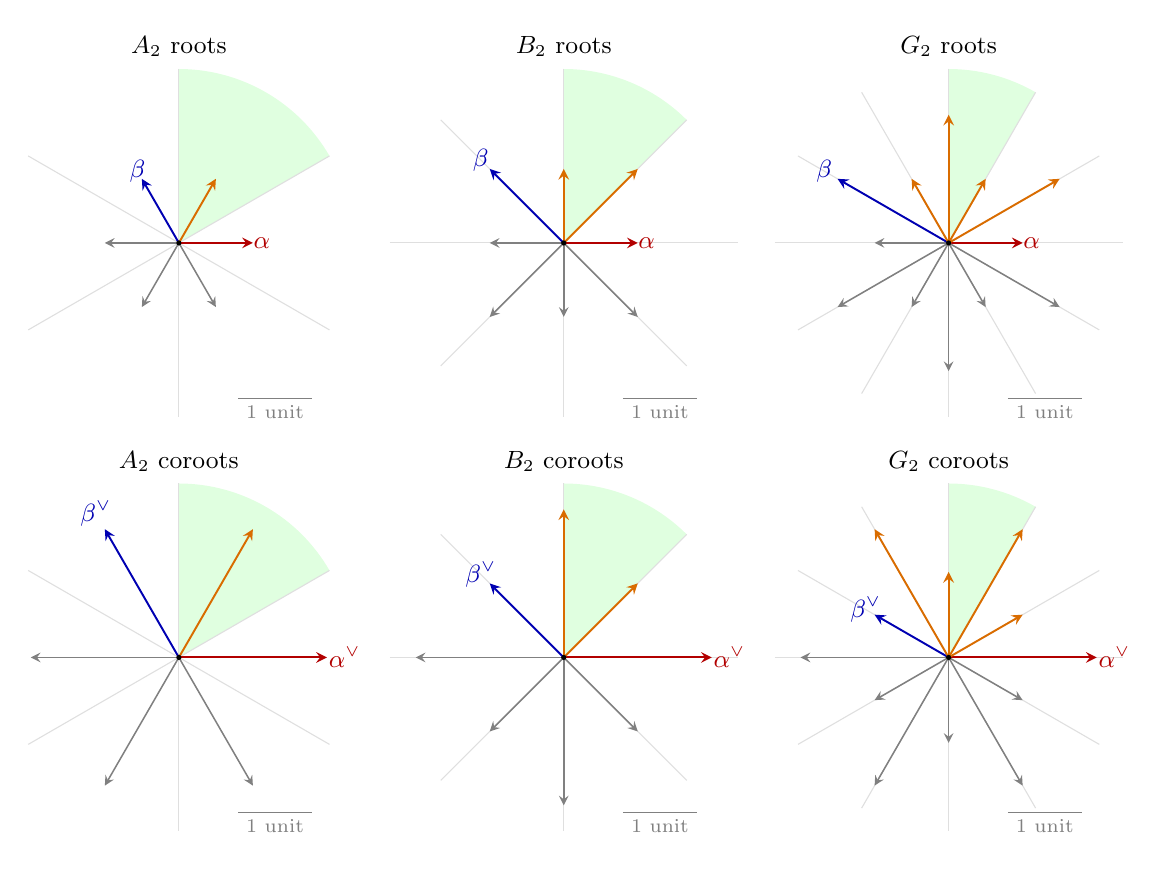
\begin{tikzpicture}[x=.94cm,y=.94cm,>=stealth,font=\small]
\begin{scope}[shift={(0.0,-0.0)}]
\path[fill=green!12] (0,0) -- (30:2.35) arc (30:90:2.35) -- cycle;
\draw[gray!25] (-0.000000000,2.350000000) -- (0.000000000,-2.350000000);
\draw[gray!25] (-2.035159699,-1.175000000) -- (2.035159699,1.175000000);
\draw[gray!25] (-2.035159699,1.175000000) -- (2.035159699,-1.175000000);
\draw[->,gray,line width=.55pt] (0,0) -- (-1.000000000,-0.000000000);
\draw[->,red!70!black,line width=.7pt] (0,0) -- (1.000000000,0.000000000);
\node[text=red!70!black] at (1.120000000,0.000000000) {$\alpha$};
\draw[->,gray,line width=.55pt] (0,0) -- (0.500000000,-0.866025404);
\draw[->,blue!70!black,line width=.7pt] (0,0) -- (-0.500000000,0.866025404);
\node[text=blue!70!black] at (-0.560000000,0.969948452) {$\beta$};
\draw[->,gray,line width=.55pt] (0,0) -- (-0.500000000,-0.866025404);
\draw[->,orange!85!black,line width=.7pt] (0,0) -- (0.500000000,0.866025404);
\fill (0,0) circle (.035);
\draw[gray] (.8,-2.1) -- (1.8,-2.1);
\node[font=\scriptsize,text=gray] at (1.3,-2.28) {1 unit};
\node at (0,2.65) {$A_2$ roots};
\end{scope}
\begin{scope}[shift={(0.0,-5.6)}]
\path[fill=green!12] (0,0) -- (30:2.35) arc (30:90:2.35) -- cycle;
\draw[gray!25] (-0.000000000,2.350000000) -- (0.000000000,-2.350000000);
\draw[gray!25] (-2.035159699,-1.175000000) -- (2.035159699,1.175000000);
\draw[gray!25] (-2.035159699,1.175000000) -- (2.035159699,-1.175000000);
\draw[->,gray,line width=.55pt] (0,0) -- (-2.000000000,-0.000000000);
\draw[->,red!70!black,line width=.7pt] (0,0) -- (2.000000000,0.000000000);
\node[text=red!70!black] at (2.240000000,0.000000000) {$\alpha^\vee$};
\draw[->,gray,line width=.55pt] (0,0) -- (1.000000000,-1.732050808);
\draw[->,blue!70!black,line width=.7pt] (0,0) -- (-1.000000000,1.732050808);
\node[text=blue!70!black] at (-1.120000000,1.939896904) {$\beta^\vee$};
\draw[->,gray,line width=.55pt] (0,0) -- (-1.000000000,-1.732050808);
\draw[->,orange!85!black,line width=.7pt] (0,0) -- (1.000000000,1.732050808);
\fill (0,0) circle (.035);
\draw[gray] (.8,-2.1) -- (1.8,-2.1);
\node[font=\scriptsize,text=gray] at (1.3,-2.28) {1 unit};
\node at (0,2.65) {$A_2$ coroots};
\end{scope}
\begin{scope}[shift={(5.2,-0.0)}]
\path[fill=green!12] (0,0) -- (45:2.35) arc (45:90:2.35) -- cycle;
\draw[gray!25] (-0.000000000,2.350000000) -- (0.000000000,-2.350000000);
\draw[gray!25] (-1.661700936,-1.661700936) -- (1.661700936,1.661700936);
\draw[gray!25] (-2.350000000,0.000000000) -- (2.350000000,-0.000000000);
\draw[gray!25] (-1.661700936,1.661700936) -- (1.661700936,-1.661700936);
\draw[->,gray,line width=.55pt] (0,0) -- (-1.000000000,-0.000000000);
\draw[->,red!70!black,line width=.7pt] (0,0) -- (1.000000000,0.000000000);
\node[text=red!70!black] at (1.120000000,0.000000000) {$\alpha$};
\draw[->,gray,line width=.55pt] (0,0) -- (1.000000000,-1.000000000);
\draw[->,blue!70!black,line width=.7pt] (0,0) -- (-1.000000000,1.000000000);
\node[text=blue!70!black] at (-1.120000000,1.120000000) {$\beta$};
\draw[->,gray,line width=.55pt] (0,0) -- (-0.000000000,-1.000000000);
\draw[->,orange!85!black,line width=.7pt] (0,0) -- (0.000000000,1.000000000);
\draw[->,gray,line width=.55pt] (0,0) -- (-1.000000000,-1.000000000);
\draw[->,orange!85!black,line width=.7pt] (0,0) -- (1.000000000,1.000000000);
\fill (0,0) circle (.035);
\draw[gray] (.8,-2.1) -- (1.8,-2.1);
\node[font=\scriptsize,text=gray] at (1.3,-2.28) {1 unit};
\node at (0,2.65) {$B_2$ roots};
\end{scope}
\begin{scope}[shift={(5.2,-5.6)}]
\path[fill=green!12] (0,0) -- (45:2.35) arc (45:90:2.35) -- cycle;
\draw[gray!25] (-0.000000000,2.350000000) -- (0.000000000,-2.350000000);
\draw[gray!25] (-1.661700936,-1.661700936) -- (1.661700936,1.661700936);
\draw[gray!25] (-2.350000000,0.000000000) -- (2.350000000,-0.000000000);
\draw[gray!25] (-1.661700936,1.661700936) -- (1.661700936,-1.661700936);
\draw[->,gray,line width=.55pt] (0,0) -- (-2.000000000,-0.000000000);
\draw[->,red!70!black,line width=.7pt] (0,0) -- (2.000000000,0.000000000);
\node[text=red!70!black] at (2.240000000,0.000000000) {$\alpha^\vee$};
\draw[->,gray,line width=.55pt] (0,0) -- (1.000000000,-1.000000000);
\draw[->,blue!70!black,line width=.7pt] (0,0) -- (-1.000000000,1.000000000);
\node[text=blue!70!black] at (-1.120000000,1.120000000) {$\beta^\vee$};
\draw[->,gray,line width=.55pt] (0,0) -- (-0.000000000,-2.000000000);
\draw[->,orange!85!black,line width=.7pt] (0,0) -- (0.000000000,2.000000000);
\draw[->,gray,line width=.55pt] (0,0) -- (-1.000000000,-1.000000000);
\draw[->,orange!85!black,line width=.7pt] (0,0) -- (1.000000000,1.000000000);
\fill (0,0) circle (.035);
\draw[gray] (.8,-2.1) -- (1.8,-2.1);
\node[font=\scriptsize,text=gray] at (1.3,-2.28) {1 unit};
\node at (0,2.65) {$B_2$ coroots};
\end{scope}
\begin{scope}[shift={(10.4,-0.0)}]
\path[fill=green!12] (0,0) -- (60:2.35) arc (60:90:2.35) -- cycle;
\draw[gray!25] (-0.000000000,2.350000000) -- (0.000000000,-2.350000000);
\draw[gray!25] (-1.175000000,-2.035159699) -- (1.175000000,2.035159699);
\draw[gray!25] (-2.035159699,-1.175000000) -- (2.035159699,1.175000000);
\draw[gray!25] (-2.035159699,1.175000000) -- (2.035159699,-1.175000000);
\draw[gray!25] (-1.175000000,2.035159699) -- (1.175000000,-2.035159699);
\draw[gray!25] (-2.350000000,0.000000000) -- (2.350000000,-0.000000000);
\draw[->,gray,line width=.55pt] (0,0) -- (-1.000000000,-0.000000000);
\draw[->,red!70!black,line width=.7pt] (0,0) -- (1.000000000,0.000000000);
\node[text=red!70!black] at (1.120000000,0.000000000) {$\alpha$};
\draw[->,gray,line width=.55pt] (0,0) -- (1.500000000,-0.866025404);
\draw[->,blue!70!black,line width=.7pt] (0,0) -- (-1.500000000,0.866025404);
\node[text=blue!70!black] at (-1.680000000,0.969948452) {$\beta$};
\draw[->,gray,line width=.55pt] (0,0) -- (0.500000000,-0.866025404);
\draw[->,orange!85!black,line width=.7pt] (0,0) -- (-0.500000000,0.866025404);
\draw[->,gray,line width=.55pt] (0,0) -- (-0.500000000,-0.866025404);
\draw[->,orange!85!black,line width=.7pt] (0,0) -- (0.500000000,0.866025404);
\draw[->,gray,line width=.55pt] (0,0) -- (-1.500000000,-0.866025404);
\draw[->,orange!85!black,line width=.7pt] (0,0) -- (1.500000000,0.866025404);
\draw[->,gray,line width=.55pt] (0,0) -- (-0.000000000,-1.732050808);
\draw[->,orange!85!black,line width=.7pt] (0,0) -- (0.000000000,1.732050808);
\fill (0,0) circle (.035);
\draw[gray] (.8,-2.1) -- (1.8,-2.1);
\node[font=\scriptsize,text=gray] at (1.3,-2.28) {1 unit};
\node at (0,2.65) {$G_2$ roots};
\end{scope}
\begin{scope}[shift={(10.4,-5.6)}]
\path[fill=green!12] (0,0) -- (60:2.35) arc (60:90:2.35) -- cycle;
\draw[gray!25] (-0.000000000,2.350000000) -- (0.000000000,-2.350000000);
\draw[gray!25] (-1.175000000,-2.035159699) -- (1.175000000,2.035159699);
\draw[gray!25] (-2.035159699,-1.175000000) -- (2.035159699,1.175000000);
\draw[gray!25] (-2.035159699,1.175000000) -- (2.035159699,-1.175000000);
\draw[gray!25] (-1.175000000,2.035159699) -- (1.175000000,-2.035159699);
\draw[gray!25] (-2.350000000,0.000000000) -- (2.350000000,-0.000000000);
\draw[->,gray,line width=.55pt] (0,0) -- (-2.000000000,-0.000000000);
\draw[->,red!70!black,line width=.7pt] (0,0) -- (2.000000000,0.000000000);
\node[text=red!70!black] at (2.240000000,0.000000000) {$\alpha^\vee$};
\draw[->,gray,line width=.55pt] (0,0) -- (1.000000000,-0.577350269);
\draw[->,blue!70!black,line width=.7pt] (0,0) -- (-1.000000000,0.577350269);
\node[text=blue!70!black] at (-1.120000000,0.646632301) {$\beta^\vee$};
\draw[->,gray,line width=.55pt] (0,0) -- (1.000000000,-1.732050808);
\draw[->,orange!85!black,line width=.7pt] (0,0) -- (-1.000000000,1.732050808);
\draw[->,gray,line width=.55pt] (0,0) -- (-1.000000000,-1.732050808);
\draw[->,orange!85!black,line width=.7pt] (0,0) -- (1.000000000,1.732050808);
\draw[->,gray,line width=.55pt] (0,0) -- (-1.000000000,-0.577350269);
\draw[->,orange!85!black,line width=.7pt] (0,0) -- (1.000000000,0.577350269);
\draw[->,gray,line width=.55pt] (0,0) -- (-0.000000000,-1.154700538);
\draw[->,orange!85!black,line width=.7pt] (0,0) -- (0.000000000,1.154700538);
\fill (0,0) circle (.035);
\draw[gray] (.8,-2.1) -- (1.8,-2.1);
\node[font=\scriptsize,text=gray] at (1.3,-2.28) {1 unit};
\node at (0,2.65) {$G_2$ coroots};
\end{scope}
\end{tikzpicture}
\end{center}

\textbf{Figure 1. Roots and coroots in rank two.} The top row uses the Euclidean coordinates \(\alpha=(1,0)\) and, respectively, \(\beta=(-1/2,\sqrt3/2)\), \((-1,1)\) and \((-3/2,\sqrt3/2)\). Red and blue mark the simple roots; orange marks the other positive roots; grey arrows are negative roots. The bottom row applies the metric identification \(r^\vee=2r/(r,r)\) from (1.2). The common scale makes the reversal of long and short lengths visible. Grey lines are reflecting hyperplanes, and the green sector consists of vectors pairing positively with both simple roots. This is a Euclidean realization of the rational spaces, not an identification of the integral character and cocharacter lattices. The definitions above and the reflection proof in Section 3 explain its mathematical content. The \href{https://kokunoyumeto.github.io/open-math-courses/courses/AG-RG/figure_sources/rank_two_roots.py}{reproducible figure source} and figure are original CC0 contributions.

\section{2. The root datum of a reductive group}\label{AG-RG-04-the-root-datum-of-a-reductive-group}

Let \(G\) be split connected reductive over a field \(k\), and let \(T\) be a split maximal torus. Take

\[
X=X^*(T),\qquad X^\vee=X_*(T),\qquad
\mathfrak g=\mathfrak t\oplus\bigoplus_{\alpha\in\Phi}\mathfrak g_\alpha.
\]

The pairing is composition of a character and a cocharacter. The preceding lesson proves that every root space is a line, that there are only the two roots \(\pm\alpha\) on its rational line, and that the rank-one map \(\varphi_\alpha:\operatorname{SL}_2\to G\) provides an intrinsic coroot with pairing two.

Choose a nonzero vector in \(\mathfrak g_\alpha\) and its linked dual in \(\mathfrak g_{-\alpha}\). Write the corresponding root parametrizations as \(x_\alpha\) and \(x_{-\alpha}\). The element

\[
n_\alpha=x_\alpha(1)x_{-\alpha}(-1)x_\alpha(1)
\tag{2.1}
\]

is the image of \(\begin{pmatrix}0&1\\-1&0\end{pmatrix}\). It normalizes \(T\). On the coroot torus it acts by inversion, and on the codimension-one torus killed by \(\alpha\) it acts trivially. These statements follow in the rank-one group and remain valid after its central quotient. On the rational character lattice they give precisely the reflection (1.1), since the two rational torus directions form an isogeny decomposition. Equality on the rational lattice is equality on the integral lattice, which is torsion-free. Thus

\[
n_\alpha t n_\alpha^{-1}
=t\,\alpha^\vee(\alpha(t)^{-1}).
\tag{2.2}
\]

Conjugation by any normalizer element permutes the root spaces and their root groups. The uniqueness of the rank-one coroot construction then permutes the coroots in the same way. Applied to (2.1), this proves both reflection axioms and their compatibility.

\textbf{Theorem 2.1.} \((X^*(T),\Phi,X_*(T),\Phi^\vee)\) is a reduced root datum. Its formation commutes with extension of the field.

\textbf{Proof.} The preceding paragraphs verify all its axioms. Reducedness is the rank-one result of the preceding lesson. A split torus has unchanged character lattice under field extension; its weight decomposition and the canonical rank-one maps extend with it. This proves the last assertion. \(\square\)

For \(\operatorname{GL}_n\), both lattices are \(\mathbf Z^n\), with dual bases \(e_i\) and \(e_i^\vee\). The roots and coroots are

\[
\alpha_{ij}=e_i-e_j,\qquad
\alpha_{ij}^\vee=e_i^\vee-e_j^\vee\quad(i\ne j).
\tag{2.3}
\]

For \(\operatorname{SL}_2\), write \(T=\{\operatorname{diag}(t,t^{-1})\}\). In the resulting copies of \(\mathbf Z\), the positive root is \(2\) and its coroot is \(1\). For \(\operatorname{PGL}_2\), use \(t\mapsto\operatorname{diag}(t,1)\) modulo scalars: the positive root is \(1\) and its coroot is \(2\). These two data are dual. Their root systems have the same two-point shape, but their integral data distinguish the groups even in characteristic two.

\section{3. Reflections and chambers}\label{AG-RG-04-reflections-and-chambers}

In \(X^\vee_\mathbf R\), remove the hyperplanes \(\langle\alpha,\lambda\rangle=0\). The connected components are \textbf{Weyl chambers}. They are open convex cones, possibly with an unrestricted central factor. A chamber determines the positive system

\[
\Phi^+_\lambda=\{\alpha:\langle\alpha,\lambda\rangle>0\}.
\tag{3.1}
\]

Conversely its signs determine the chamber. Each chamber contains a rational point, and therefore an integral cocharacter after multiplication by a positive integer.

The reflection group is transitive on the chambers. To prove this, connect interior points of two chambers by a polygonal path that crosses only one hyperplane at a time and never their pairwise intersections. Such a path exists after a small perturbation. At a crossing, the reflection in that hyperplane interchanges the two adjacent chambers: choose a point of the wall on no other hyperplane, and a sufficiently small ball around it; the reflection reverses the normal direction and permutes the entire hyperplane arrangement. Successive reflections carry the first chamber to the last. This argument proves transitivity without assuming the normalizer calculation that follows.

We will also use the elementary description of simple roots. In a positive system, a positive root is \textbf{simple} if it is not a sum of two positive roots. The simple roots form a basis of \(\mathbf R\Phi\), and every positive root is a nonnegative integral combination of them. Here are the combinatorial details.

First, for nonparallel roots \(a,b\), if \((a,b)>0\), at least one of \(a-b\) and \(b-a\) is a root. This can be checked within their two-dimensional root system. The complete reduced crystallographic possibilities, with \(a\) chosen short in the last two, have positive roots

\[
\begin{array}{c|l}
A_1\times A_1&a,b\\
A_2&a,b,a+b\\
B_2&a,b,a+b,2a+b\\
G_2&a,b,a+b,2a+b,3a+b,3a+2b.
\end{array}
\tag{3.2}
\]

For completeness, this list follows from the reflection axioms, rather than an algebraic-group classification. Two adjacent root lines make an angle \(\theta\) for which the product of the two integral Cartan numbers is \(4\cos^2\theta\). It is a nonnegative integer less than four. The successive reflections in adjacent lines fill their finite dihedral orbit, so the adjacent angles are respectively \(\pi/2,\pi/3,\pi/4,\pi/6\). In the odd case all lines are one orbit and have equal root lengths. In the even nonorthogonal cases there are two orbits; the two Cartan numbers force the squared length ratios two and three. Reflecting two adjacent roots now gives exactly the sets (3.2) and their negatives. Checking subtraction in these displayed sets gives the assertion for every pair; orthogonal pairs have zero inner product and need no assertion.

Distinct simple roots consequently have nonpositive inner product: otherwise the positive one of their differences would decompose one of them. They are linearly independent. Indeed, a linear dependence can be separated into an equality of positive linear combinations with disjoint supports. The inner product of the two sides is nonpositive, while their common squared norm is positive unless both are zero. Applying the chamber functional excludes a nonempty positive combination equal to zero. Finally, decompose any nonsimple positive root into two positive roots and repeat. There is no infinite descent, since the chamber functional has a positive minimum on the finite positive root set. This gives a nonnegative integral expansion in the simple roots and proves spanning.

If \(\alpha\) is simple, \(s_\alpha\) permutes \(\Phi^+\setminus\{\alpha\}\). In the simple-root expansion of a different positive root, at least one other coefficient is nonzero; reflection changes only the coefficient of \(\alpha\). All coefficients of a root have the same sign, so the reflected root remains positive. The walls of the chamber are therefore its simple-root walls. The reflections in these walls generate the whole reflection group: their subgroup is already transitive on chambers by the crossing argument, and every root wall becomes a wall of the initial chamber after such a transport. Every root reflection is consequently conjugate to a simple-root reflection in that subgroup.

\subsection{Length and standard parabolic cosets}\label{AG-RG-04-length-and-standard-parabolic-cosets}

We first prove the reflection assertion entirely in the root space, before using any group normalizer. This also makes the length and word results available for every reduced root datum.

\textbf{Lemma 3.A (a chamber has trivial stabilizer).} The reflection group acts freely on chambers.

\textbf{Proof.} For an empty root set the group is the identity, so the assertion holds. Otherwise work in the Euclidean root space, discarding the central factor, on which all reflections act trivially. Reflection across a wall carries either adjacent chamber to the other. Starting with a fixed chamber \(C\), a path crossing one wall at a time therefore transports \(C\) by a product of the crossed-wall reflections. If the current transport is \(v\), a wall of \(vC\) is \(v\) applied to a simple wall of \(C\); crossing it replaces \(v\) by \(vs_i\). Thus words in the simple reflections and such wall galleries give the same transports.

We show that a closed gallery has identity transport. Realize it by a polygonal loop avoiding intersections of two hyperplanes at its crossings. Fill the loop by a polygonal disk in the root space; for example join each of its edges to an auxiliary interior vertex. Subdivide and perturb the interior vertices slightly. Because there are finitely many hyperplanes, the vertices can be chosen so that the disk avoids their intersections of codimension at least three, meets each codimension-two intersection transversely in finitely many interior points, and crosses single hyperplanes transversely away from these points. These choices exclude finitely many proper algebraic conditions on the perturbations. Intersections of codimension greater than two can be avoided by a two-dimensional disk; the same statement in dimensions one and two has no such intersections to avoid.

The inverse images of the walls now divide the disk into regions. Passing a path across an ordinary wall arc and back inserts two copies of the same reflection, whose product is the identity. Passing across an intersection point changes its gallery by the small circuit around that point. Its walls have normals in the two-dimensional orthogonal complement of the intersection. The roots in this plane form exactly one of the rank-two systems (3.2). By the calculation preceding that list, consecutive reflecting lines have angle \(\pi/m\), for \(m=2,3,4,6\). The \(2m\) successive crossings around a small full circle have product the identity: consecutive pairs rotate this plane by \(2\pi/m\), and \(m\) such pairs make a full rotation. Every factor fixes the common orthogonal complement, so the product is the identity on the whole root space. The orientation-reversed circuit has the inverse product and gives the same conclusion.

To see that these are all changes needed, cut the disk along disjoint arcs from its finitely many intersection points to its boundary. In the cut polygon any closed path can be reduced by successively removing its innermost crossings of wall arcs. Restoring each cut inserts the corresponding small circuit or its inverse. Hence the boundary gallery has identity transport, by the two calculations just given. In dimension one a loop consists directly of back-and-forth crossings and has the same conclusion.

Suppose \(wC=C\). Choose a word for \(w\) in simple reflections. Its successive chambers give a gallery from \(C\) back to \(C\). Join the two endpoint representatives inside the convex chamber, producing a closed gallery without an additional crossing. Its transport is \(w\), so the preceding argument gives \(w=1\) on the root space. Section 1 proved that this action determines \(w\) on the full lattice. Thus \(w=1\). \(\square\)

The cell dimensions below now follow from this independent chamber proof. No normalizer identification is used in the length calculation.

\textbf{Proposition 3.1.} Let \(\ell(w)\) be the minimum number of simple reflections in an expression for \(w\). Then \(\ell(w)=|\Psi_w|\), where \(\Psi_w=\{\alpha\in\Phi^+:w^{-1}\alpha<0\}\). For \(J\subset\Delta\), each right coset of \(W_J=\langle s_\alpha:\alpha\in J\rangle\) has a unique element \(w\) of minimum length. It is characterized by \(w(\Phi_J^+)\subset\Phi^+\). For this \(w\) and every \(z\in W_J\),

\[
\Psi_{wz}=\Psi_w\sqcup w\Psi_z,
\qquad \ell(wz)=\ell(w)+\ell(z).
\]

\textbf{Proof.} Fix the positive chamber \(C\). A word in simple reflections gives a gallery of adjacent chambers from \(C\) to \(wC\): if the current chamber is \(vC\), its wall corresponding to a simple root leads to \(vs_\alpha C\). Every such gallery must cross each hyperplane separating \(C\) from \(wC\). There are \(|\Psi_w|\) of these, since the sign of a positive root on \(wC\) is the sign of \(w^{-1}\alpha\) on \(C\).

Conversely choose interior points of \(C\) and \(wC\) generically, so the straight segment between them never meets an intersection of distinct root hyperplanes. A hyperplane with endpoints on the same side is not crossed; each separating hyperplane is crossed exactly once. The segment therefore supplies a gallery with \(|\Psi_w|\) steps. Write its successive chambers as \(vC\) by the preceding adjacent-wall rule. At the end, \(vC=wC\); freeness from Lemma 3.A gives \(v=w\). Thus the gallery supplies a word of that length and proves the length formula. The same wall calculation gives \(\ell(ws_\alpha)=\ell(w)+1\) or \(\ell(w)-1\) according as \(w\alpha\) is positive or negative.

Choose a minimum-length element \(w\) of a right coset, which exists because \(W\) is finite. The last calculation gives \(w\alpha>0\) for every \(\alpha\in J\). Every root in \(\Phi_J^+\) is a nonnegative integral combination of those simple roots; its image is consequently positive. Thus \(w(\Phi_J^+)\subset\Phi^+\).

Each generator of \(W_J\) changes only the coefficient of its own simple root in a root's simple-root expansion. A positive root outside \(\Phi_J\) has a positive coefficient outside \(J\), which remains unchanged. Since all coefficients of a root have the same sign, every element of \(W_J\) preserves its positivity. The corresponding assertion holds for negative roots outside \(\Phi_J\). In particular \(\Psi_z\subset\Phi_J^+\) for \(z\in W_J\).

Now suppose \(w\) sends \(\Phi_J^+\) to positive roots. If \(\alpha\in\Psi_w\), then \(w^{-1}\alpha\) is negative and outside the Levi subsystem: a negative Levi root would have negative image under \(w\), whereas \(\alpha\) is positive. Applying \(z^{-1}\) therefore leaves it negative. If \(\alpha\notin\Psi_w\) is positive, then \(w^{-1}\alpha\) is positive, and \(z^{-1}w^{-1}\alpha\) is negative precisely when \(w^{-1}\alpha\in\Psi_z\). These two cases prove the displayed disjoint inversion-root identity. Its cardinalities and the length formula prove length additivity. They also show that any element with the positive-Levi condition is a minimum in its right coset.

Finally, if two such minima satisfy \(w'=wz\), applying additivity in both directions gives \(\ell(w')=\ell(w)+\ell(z)\) and \(\ell(w)=\ell(w')+\ell(z^{-1})\). Since \(\ell(z^{-1})=\ell(z)\), we get \(\ell(z)=0\) and \(z=1\). This proves uniqueness. \(\square\)

\subsection{Relations between reflection words}\label{AG-RG-04-relations-between-reflection-words}

The same length calculation determines all relations between simple reflections. This is the Coxeter presentation used in the pinned isomorphism argument of the next lesson. Its inputs are the rank-two root calculation (3.2), chamber freeness in Lemma 3.A, and the standard-parabolic coset calculation in Proposition 3.1. The proof below applies to every reduced root datum, including its central lattice directions.

For distinct simple roots \(\alpha_i,\alpha_j\), put \(c_{ij}=\langle\alpha_i,\alpha_j^\vee\rangle\langle\alpha_j,\alpha_i^\vee\rangle\). The invariant positive definite form gives \(c_{ij}=4\cos^2\theta\), where \(\theta\) is the obtuse angle between these roots. The rank-two calculation (3.2) gives \(c_{ij}=0,1,2,3\) and \(m_{ij}=2,3,4,6\), respectively. On the plane spanned by these roots, the product \(s_i s_j\) is a rotation through \(2\pi/m_{ij}\), up to orientation, and on its orthogonal complement it is the identity. Hence it has order \(m_{ij}\). The group \(W_{ij}=\langle s_i,s_j\rangle\) consists of the \(m_{ij}\) rotations \((s_i s_j)^a\) and the \(m_{ij}\) reflections \((s_i s_j)^a s_i\).

After cancelling adjacent equal letters, words in two involutions alternate. Write \(R=s_i s_j\). Alternating words of length \(2a\) are \(R^a\) and \(R^{-a}\), while those of length \(2a+1\) are \(R^a s_i\) and \(R^{-a-1}s_i\). Comparing these exponents modulo \(m_{ij}\) shows that all alternating words of length less than \(m_{ij}\) are distinct and reduced. The two alternating words of length \(m_{ij}\) agree and give the unique longest element. These words exhaust the \(2m_{ij}\) elements: there is one empty word, two words at each length \(1,\ldots,m_{ij}-1\), and one element at length \(m_{ij}\).

A \textbf{braid move} replaces either alternating block of length \(m_{ij}\) by the other. With the involution relations, it is equivalent to \((s_i s_j)^{m_{ij}}=1\).

\textbf{Lemma 3.2 (two left descents).} If both \(s_i\) and \(s_j\) shorten \(w\) on the left, there is a length-additive factorization \(w=v_0u\), where \(v_0\) is the longest element of \(W_{ij}\) and \(u\) has minimum length in \(W_{ij}w\).

\textbf{Proof.} Invert the unique minimum representative assertion of Proposition 3.1 to obtain the left-coset version. It gives \(w=vu\), \(v\in W_{ij}\), with \(u^{-1}(\Phi_{ij}^+)\subset\Phi^+\) and \(\ell(vu)=\ell(v)+\ell(u)\). A positive root outside \(\Phi_{ij}\) has a positive coefficient on some other simple root; neither \(s_i\) nor \(s_j\) changes that coefficient. Such a root remains positive under \(W_{ij}\), so the ambient length of \(v\) equals its rank-two length.

For \(k=i,j\), the root \(v^{-1}\alpha_k\) belongs to \(\Phi_{ij}\), and \(u^{-1}\) preserves its sign. Thus \(w^{-1}\alpha_k<0\) implies \(v^{-1}\alpha_k<0\). Every positive root in \(\Phi_{ij}\) is a nonnegative combination of \(\alpha_i,\alpha_j\), so \(v^{-1}\) makes all of them negative. Its length is consequently the number of rank-two positive roots. This is the rank-two longest element just calculated. \(\square\)

\textbf{Lemma 3.3 (reduced words).} Any two reduced words for the same element are connected by braid moves.

\textbf{Proof.} Induct on the length \(k\). If the first letters agree, cancel them, apply induction to the two tails of length \(k-1\), and restore the first letter. Otherwise the two first letters are \(s_i\ne s_j\), so both shorten \(w\) on the left. Lemma 3.2 gives \(w=v_0u\), with \(\ell(w)=m_{ij}+\ell(u)\). Fix a reduced word for \(u\). Prefix it with either alternating length-\(m_{ij}\) word for \(v_0\). Both resulting words are reduced; one starts with \(s_i\), the other with \(s_j\). After cancelling the first \(s_i\), induction connects the first original word to the first constructed word. The same induction with \(s_j\) treats the second original word. A single braid move connects the two constructed prefixes. Composing these moves proves the assertion. \(\square\)

\textbf{Theorem 3.4 (Coxeter presentation).} For the Weyl group of the root datum under consideration,

\[
W=\langle s_i\mid s_i^2=1,\ (s_i s_j)^{m_{ij}}=1\ (i\ne j)\rangle.
\]

\textbf{Proof.} The relations hold by the reflection and rank-two calculations, so the presented group surjects onto \(W\). Reduce an arbitrary word by induction on its number of letters. First reduce its prefix to a reduced word for its value \(a\). If the final letter \(s_i\) increases length, the word is reduced. If it decreases length, choose a reduced word \(A\) for \(as_i\). Then \(A s_i\) is reduced for \(a\), by Proposition 3.1. Lemma 3.3 changes the reduced prefix to \(A s_i\) by braid moves. The entire word becomes \(A s_i s_i\), and the involution relation cancels the last two letters. Thus the given relations turn every word into a reduced word for its actual value. A word representing \(1\) reduces to the empty word. The kernel is zero. \(\square\)

The argument applies to the full character lattice, including its central summand: reflections fix that summand, and the faithful action on the root span in Section 1 determines their relations.

\section{4. Borel subgroups are positive systems}\label{AG-RG-04-borel-subgroups-are-positive-systems}

We first work over an algebraic closure. A Borel subgroup \(B\) containing \(T\) contains exactly one of \(U_\alpha,U_{-\alpha}\) for every root. Indeed, \(B\cap C_G(T_\alpha)\) is a Borel subgroup of the rank-one centralizer, by the centralizer--Borel argument of the preceding lesson. There its two possibilities are the two triangular subgroups constructed in rank one. In particular,

\[
\dim B=\dim T+\tfrac12|\Phi|.
\tag{4.1}
\]

For an integral cocharacter \(\lambda\) in a chamber, the limit construction gives

\[
L_G(\lambda)=T,\qquad
P_G(\lambda)=T\ltimes U_G(\lambda),
\qquad
\operatorname{Lie}U_G(\lambda)
=\bigoplus_{\langle\alpha,\lambda\rangle>0}\mathfrak g_\alpha.
\tag{4.2}
\]

The equality \(L_G(\lambda)=T\) follows because the smooth connected centralizer has Lie algebra \(\mathfrak t\). The second group is connected solvable and hence lies in a Borel subgroup. Its dimension is (4.1), so it is that Borel subgroup. The root groups of positive sign lie in \(U_G(\lambda)\): their rank-one parametrizations are multiplied by \(t^{\langle\alpha,\lambda\rangle}\), which tends to zero. Thus \(P_G(\lambda)\) depends only on the chamber. Conversely, two such subgroups with different signs have different Lie algebras, so their chambers are different.

Every Borel containing \(T\) arises this way. Choose one \(P_G(\lambda)\). The normalizer quotient acts transitively on Borels containing \(T\), by the earlier torus conjugacy argument. If \(n\) carries this subgroup to \(B\), then it carries the cocharacter to \(n\lambda n^{-1}\) and (4.2) to the Lie algebra of \(B\). Thus \(B=P_G(n\lambda n^{-1})\).

The construction is defined over \(k\) because \(T\) is split and \(\lambda\) is integral in its character-dual lattice. Geometric equality of the resulting smooth closed subgroups descends. It follows that all the geometric Borels containing \(T\) are defined over \(k\).

\textbf{Theorem 4.1.} For a split reductive group over any field, Borels containing its split maximal torus correspond bijectively to positive systems. The normalizer Weyl group equals the reflection Weyl group and acts simply transitively on these systems.

\textbf{Proof.} We have proved the correspondence, and it respects the normalizer action. Each root reflection is represented by (2.1), so the reflection group embeds in the normalizer quotient. It is transitive on chambers by Section 3. The normalizer quotient is simply transitive on the corresponding Borels: a normalizer element fixing a Borel lies in \(N_G(B)\cap N_G(T)=B\cap N_G(T)=T\). Hence a transitive subgroup of this simply transitive permutation group must be the whole group. This proves both equality and freeness. Products of (2.1) give representatives \(n_w\in N_G(T)(k)\) for every \(w\). \(\square\)

\textbf{Theorem 4.2 (the relative Weyl scheme).} \(W_G(T)\) is represented by a finite étale group scheme over \(S\).

\textbf{Proof.} We prove representability directly as a functor before forming a quotient. Work on an étale cover on which \(T=D_S(X)\) is split, and then on open subsets on which the finite roots and coroots are constant. The weight summands of \(\operatorname{Lie}G\) have locally constant ranks, and coroots are locally constant lattice maps by \emph{Diagonalizable groups}, Proposition 7.4. Choose a positive base and trivialize its finitely many simple root lines. All these choices are available on this cover; no global pinning is required.

The earlier AG-RG-03 Theorems 4.1 and 7.1 provide the paired root parameters and the rank-one \(\operatorname{SL}_2\) homomorphism. For a simple root define \(n_\alpha=x_\alpha(1)x_{-\alpha}(-1)x_\alpha(1)\). It normalizes \(T\): in \(G_\alpha\) the preimage of its adjoint diagonal torus is \(T\), and the rank-one matrix normalizes that torus. Its action on \(T\) is the reflection \[
n_\alpha t n_\alpha^{-1}=t\,\alpha^\vee(\alpha(t)^{-1}).
\] This identity holds on all test schemes. To verify it without discarding central or nilpotent elements, lift \(\alpha(t)\) fppf locally through the square map on \(\mathbf G_m\), say \(\alpha(t)=r^2\). Then \(t=z\alpha^\vee(r)\) with \(z\in\ker\alpha=Z(G_\alpha)\), and the rank-one matrix sends \(\alpha^\vee(r)\) to \(\alpha^\vee(r^{-1})\). This gives the formula locally and hence by descent. The square cover is faithfully flat even in characteristic two.

For every element \(w\) of the finite reflection group from Section 3, choose one simple-reflection word and multiply its \(n_\alpha\) to obtain a section \(n_w\) with that action on \(X\). No independence of the chosen word is needed. Theorem 4.1 identifies, on every geometric fibre, the normalizer's torus action with exactly this reflection group, including its action on the full character lattice.

Now let \(S'\to S\) be any test scheme and \(n\in N_G(T)(S')\). Proposition 7.4 represents automorphisms of \(D_{S'}(X)\) by the discrete constant scheme \(\operatorname{Aut}(X)_{S'}\). Thus the action of \(n\) is a locally constant lattice automorphism. Its value at every geometric point is in the finite subset \(W\), by Theorem 4.1. A locally constant map to a discrete scheme therefore factors through \(W_{S'}\) on the whole test scheme, including its nilpotents. On the open and closed region labelled \(w\), the element \(n_w^{-1}n\) centralizes \(T\), and the earlier AG-RG-02 Theorem 2.2 identifies this schematic centralizer with \(T\). Conversely every \(n_wt\) normalizes \(T\). We have proved an isomorphism of functors \[
\coprod_{w\in W}T\xrightarrow{\sim}N_G(T),\qquad (w,t)\longmapsto n_wt.
\] Its inverse is the locally constant action label together with \(n_w^{-1}n\). In particular the normalizer is represented and smooth on this cover. Right multiplication by \(T\) acts within each labelled copy, so its fppf quotient is exactly the constant finite étale scheme \(W_S\) there.

On overlaps these quotients represent the same fppf normalizer-quotient sheaf, so their unique identifications satisfy the cocycle identity and respect multiplication. Effective affine algebra descent, proved at the beginning of \emph{Quotients and torsors}, glues them to a group scheme over \(S\). Finite locally free algebras descend by the finite-presentation and finite-projectivity descent proofs; here their local algebras are finite products of the base algebra. Étaleness also descends: over a square-zero test extension the local constant finite schemes have unique lifts, and uniqueness makes these lifts agree on the faithfully flat overlaps. Thus the descended finite-presentation algebra is formally étale. The quotient is finite étale over the original arbitrary base. \(\square\)

\section{5. Coordinates on the unipotent radicals}\label{AG-RG-04-coordinates-on-the-unipotent-radicals}

We need actual scheme coordinates, rather than only equality of dimensions. The following graded argument works over a base ring \(R\) as well as over a field.

\textbf{Lemma 5.1.} Suppose a smooth affine \(R\)-scheme \(Y\) of finite presentation has a section \(e\) and a \(\mathbf G_m\)-action which extends to \(\mathbf A^1\) and sends \(0\times Y\) to \(e\). Suppose the tangent module at \(e\) is free with positive weights \(d_1,\ldots,d_N\). A \(\mathbf G_m\)-equivariant map from \(\mathbf A_R^N\), with these weights, to \(Y\) whose differential at zero is an isomorphism is an isomorphism.

\textbf{Proof.} Write \(A=\Gamma(Y,\mathcal O_Y)\). Extension of the action gives a nonnegative grading. Contraction to \(e\) makes \(A_0=R\), and the augmentation ideal is \(I=\bigoplus_{d>0}A_d\). Choose finitely many homogeneous algebra generators; their positive degrees imply that the degree filtration and the \(I\)-adic filtration are cofinal. Thus completion retains every finite degree component faithfully.

The given map is étale along the zero section, since both schemes are smooth and its differential is invertible there. Equivalently, in coordinates its invertible linear term allows unique successive solution modulo \(I^m\): once a solution is known modulo \(I^m\), the next correction is the solution of the same invertible linear system in \(I^m/I^{m+1}\). It induces an isomorphism on the formal completions at the sections. The isomorphism respects degrees. Restricting it and its inverse to each finite degree component, and then taking their direct sums, gives an isomorphism of the original graded algebras. This proves the assertion. \(\square\)

For any ordering \(\alpha_1,\ldots,\alpha_N\) of \(\Phi^+\), multiplication gives

\[
\prod_i U_{\alpha_i}\xrightarrow{\sim}U_G(\lambda).
\tag{5.1}
\]

Indeed both sides are contracted by \(\lambda\), and the differential is the direct-sum identification of their distinct root lines. After trivializing these lines, Lemma 5.1 applies; the result descends from these local trivializations. We denote the group by \(U^+\), independently of the ordering. Applying the same argument to \(-\lambda\) and using the open immersion in the preceding lesson gives the \textbf{big cell}

\[
U^-\times T\times U^+\hookrightarrow G.
\tag{5.2}
\]

The inverse of (5.1) provides root coordinates. For roots \(a,b\) with \(b\ne\pm a\), choose a positive system containing them. The commutator has the form

\[
[x_a(u),x_b(v)]
=\prod_{ia+jb\in\Phi,\ i,j>0}
x_{ia+jb}(C_{ij}u^iv^j).
\tag{5.3}
\]

Here the order is fixed, and the coefficients depend on the parametrizations and order. To prove the formula, take any root coordinate of the commutator. It is a polynomial in \(u,v\), equivariant for \(T\). Its monomials must have weight equal to that root. Setting either variable to zero makes the commutator one, so both exponents must be positive. Since \(a,b\) are linearly independent, the exponents for a given target root are unique. This proves (5.3), including over rings with nilpotents; distinct torus characters are distinct homogeneous degrees, so no cancellation by a characteristic is involved.

We shall need root subsets \(\Psi=\Phi^+\cap C\) where \(C\) is closed under addition. Setting the coordinates outside \(\Psi\) to zero in (5.1) gives a smooth closed subgroup \(U_\Psi\), directly parametrized by the groups in \(\Psi\) in any order. To check the subgroup assertion, use the torus-equivariant coordinate polynomials for multiplication and inversion. Every nonconstant monomial has target weight equal to the sum of its input weights. A sum of weights in \(C\) is in \(C\), so a coordinate outside \(\Psi\) remains zero. Different orderings give the same subgroup: in the coordinates of one ordering the product in another has no component outside \(\Psi\), and its invertible differential and contraction give an isomorphism by Lemma 5.1.

In particular this applies to the two subsets

\[
\Psi_w=\Phi^+\cap w\Phi^- ,\qquad
\Theta_w=\Phi^+\cap w\Phi^+.
\tag{5.4}
\]

Their cones are the intersections of two open linear half-spaces. Ordering the first subset before the second in (5.1) gives \(U^+=U_{\Psi_w}U_{\Theta_w}\) as a product of schemes.

\section{6. The Bruhat cells from a projective limit}\label{AG-RG-04-the-bruhat-cells-from-a-projective-limit}

We spell out the projective geometric argument used here.

\textbf{Lemma 6.1.} Let a \(\mathbf G_m\) act on a smooth projective variety with an equivariant projective embedding. Suppose its fixed points are isolated. The points whose limit at zero is a fixed point \(p\) form an affine locally closed scheme \(Y_p\), contracted to \(p\), and its tangent space at \(p\) is the positive-weight part of \(T_pY\). An equivariant map from a positive-weight affine space to \(Y_p\), with invertible differential at zero, is an isomorphism.

\textbf{Proof.} Diagonalize the action on the vector space of the embedding. Represent \(p\) by an eigenvector of weight \(m\) and choose one of its nonzero coordinates. In the corresponding affine chart, the limit is \(p\) precisely when all coordinates of weight less than \(m\) vanish and all ratios of weight \(m\) coordinates equal their values at \(p\). The remaining coordinates have strictly positive relative weights. Intersect this affine linear space with the projective variety. This constructs \(Y_p\) as a closed subscheme of an affine space, with the stated limit condition.

At \(p\), choose homogeneous formal parameters in the smooth completed local ring; this is possible by the weight decomposition and lifting a basis of the cotangent space. The limit equations set the negative-weight parameters to zero. There are no zero-weight parameters because the fixed scheme is smooth with zero tangent dimension. Thus the completed local ring of \(Y_p\) is the formal power-series ring in the positive parameters. It is smooth at \(p\) and has the asserted tangent space. The nonsmooth locus of \(Y_p\) would be a closed invariant subset. If nonempty, contraction would put \(p\) in it, a contradiction. Hence \(Y_p\) is smooth everywhere. Lemma 5.1 proves the last assertion. These constructions commute with extension of the field. \(\square\)

Let \(B\) correspond to \(\Phi^+\) and choose an integral cocharacter \(\lambda\) in its chamber. The projective variety \(G/B\) has an equivariant projective embedding, from the ample homogeneous line bundle in the quotient construction of the preceding lesson. Its \(T\)-fixed points are the points \(n_wB\), \(w\in W\). To see this, a fixed coset represents a Borel containing \(T\), and Theorem 4.1 applies.

There are no additional fixed points of \(\lambda\). Each connected component of the proper fixed scheme is \(T\)-stable and therefore contains a \(T\)-fixed point by the torus fixed-point theorem. At such a point the tangent weights are roots, all nonzero on \(\lambda\). Its fixed tangent space is zero. Smoothness of fixed schemes for a torus then makes the component a point. The fixed scheme is consequently the same finite reduced set \(\{n_wB\}\).

At \(n_wB\), the tangent weights of \(G/B\) are \(\Phi\setminus w\Phi^+\), with the toral summand removed. Its positive-weight part is precisely

\[
\bigoplus_{\alpha\in\Psi_w}\mathfrak g_\alpha.
\]

The map \(U_{\Psi_w}\to G/B\), \(u\mapsto un_wB\), lands in the attracting scheme of this point. It is equivariant and its differential is the displayed isomorphism. Lemma 6.1 therefore gives an isomorphism

\[
U_{\Psi_w}\xrightarrow{\sim}(G/B)_{n_wB}^+.
\tag{6.1}
\]

Every geometric point of a projective variety has a limit under \(\lambda(t)\) as \(t\to0\), as follows directly from the least nonzero weight in its projective coordinates. That limit is fixed and unique. Thus the schemes (6.1) are disjoint locally closed strata covering \(G/B\).

They are also exactly its \(B\)-orbits. In (5.4), \(U_{\Theta_w}\) fixes \(n_wB\), since each of its root groups is contained in \(n_wBn_w^{-1}\). The torus fixes the same point. The product decomposition of \(U^+\) therefore shows

\[
Bn_wB/B=U_{\Psi_w}n_wB/B.
\]

Pull back the principal \(B\)-bundle \(G\to G/B\) to this stratum. It has the section \(u\mapsto un_w\), so it is trivial. We obtain an isomorphism of locally closed schemes

\[
U_{\Psi_w}\times B\xrightarrow{\sim}Bn_wB,
\qquad (u,b)\longmapsto un_wb.
\tag{6.2}
\]

\textbf{Theorem 6.2 (Bruhat decomposition).} For a split connected reductive group over any field \(k\),

\[
G=\coprod_{w\in W}Bn_wB
\quad\text{as a locally closed stratification},
\qquad
G(k)=\coprod_{w\in W}B(k)n_wB(k).
\tag{6.3}
\]

Moreover \(Bn_wB\) has dimension \(\dim B+|\Psi_w|\), and its quotient by the right \(B\)-action is an affine space of dimension \(|\Psi_w|\).

\textbf{Proof.} The geometric stratification and the scheme isomorphisms were just proved. They are defined over \(k\): the root groups, cocharacter, and representatives (2.1) all are. For \(g\in G(k)\) its image in \(G/B\) belongs to exactly one stratum; the inverse of (6.1) is defined over \(k\), so it supplies \(u\in U_{\Psi_w}(k)\). Equality of the two cosets means \((un_w)^{-1}g\in B(k)\). This proves (6.3) without assuming that rational points are dense or that the field is infinite. Conversely (6.2) makes every such product a point of the indicated stratum. Its dimension and affine-space assertion follow from (5.1). \(\square\)

The disjoint-union notation in (6.3) describes strata and points. It does not assert that the cells are open-and-closed components, or that a morphism from a general scheme lands in one cell globally. In \(\operatorname{SL}_2\) the two cells have dimensions two and three, and the latter is open dense.

\section{7. Central quotients and their root coordinates}\label{AG-RG-04-central-quotients-and-their-root-coordinates}

\textbf{Theorem 7.1.} Let \(G\) be reductive over \(S\) and \(H\subset Z(G)\) a closed subgroup of multiplicative type of finite presentation. Its affine reductive quotient \(G/H\), constructed in the preceding lesson, Theorem 1.1, commutes with every base change. For a split maximal torus \(T\) its maximal torus is \(T/H\), and its root groups are the images of those of \(G\).

\textbf{Proof.} The preceding lesson proves the affine quotient, torsor, finite-presentation, arbitrary-base-change and reductivity assertions. We now prove the additional coordinate assertions, using the root groups already constructed.

Finally, after making \(T\) split, \(H\subset T\), and \(T/H\) is a torus: its characters are the kernel of \(X^*(T)\to X^*(H)\), a free sublattice. The big cell is \(H\)-stable, with \(H\) acting only on its torus factor. Its quotient is the open subscheme

\[
U^-\times(T/H)\times U^+\subset Q.
\tag{7.1}
\]

Root groups intersect \(H\) trivially and hence embed in \(Q\). Their images are closed: the inverse image of such an image is \(H U_\alpha\), a closed subscheme of the triangular rank-one subgroup, and closedness descends along \(q\). The cells (7.1) show that their weights are the same roots, now regarded as characters of \(T/H\). There are no additional zero weights, so \(T/H\) is a maximal torus by the centralizer criterion. Everything constructed by invariants commutes with base change, and the local constructions glue uniquely as fppf quotients. \(\square\)

The only general morphism tools used in this proof are the fibre criteria for flatness, smoothness and étaleness: a finite-presentation morphism between schemes flat over the same base is flat if its fibre morphisms are flat; a flat finite-presentation morphism with smooth (respectively étale) fibres is smooth (respectively étale). These are general algebraic-geometry prerequisites, not reductive-group classification results.

\section{8. Splittings and subgroup constructions in families}\label{AG-RG-04-splittings-and-subgroup-constructions-in-families}

Over a scheme, saying that a maximal torus is split does not trivialize its root lines. We call a reductive group \textbf{split with specified root datum} when its maximal torus is identified with \(D_S(X)\), its root datum is the indicated constant datum, and its root lines are trivializable. A \textbf{pinning} additionally chooses a nowhere-vanishing section in each simple root line. These are the objects classified in the next lesson.

Every reductive group acquires such a splitting and a pinning étale locally. The second lesson, Theorem 2.3, provides a maximal torus; the first lesson provides its étale splitting. Its finite weight decomposition has locally constant ranks; the root set can therefore be made constant after an open localization. Coroots are sections of the locally constant cocharacter sheaf and can likewise be made constant. Trivialize the finitely many simple root lines on a further open cover. The root groups and rank-one constructions then supply the pinning. No assumption that the original base is reduced is used.

The coordinate proof in Section 5 works over this cover and descends without chosen parametrizations. Thus for a positive system the product of its root \textbf{line bundles} is \(U^+\), and (5.2) is an open immersion over the base. For a cocharacter \(\lambda\), the smooth closed subgroup \(P_G(\lambda)\) has roots of nonnegative pairing; its Levi subgroup \(L_G(\lambda)\) has roots of zero pairing and is reductive, being a torus centralizer. Its unipotent subgroup \(U_G(\lambda)\) has roots of positive pairing. The limit homomorphism gives the actual Levi decomposition \(P_G(\lambda)=L_G(\lambda)\ltimes U_G(\lambda)\). Relative parabolic quotients and their parameter scheme are the subject of the last lesson.

For the quotient in Theorem 7.1, the root datum is especially transparent. Let \(X'=\ker(X\to X^*(H))\). The roots lie in \(X'\) because \(H\) is central. Characters change from \(X\) to \(X'\), cocharacters by the dual map, and each coroot becomes its image under \(T\to T/H\). The pairing with every root remains two. A central quotient can change the integral lattice without changing the root system.

The torus example warns against silently choosing one datum on a disconnected base. On one component take \(\mathbf G_m\) and on another take \(\mathbf G_m^2\). This is a reductive group with no single constant character lattice on the whole base. All constant-datum statements are made componentwise or on the explicitly stated covers.

\subsection{Bruhat cells over a base}\label{AG-RG-04-bruhat-cells-over-a-base}

The field theorem also gives actual cells over the integers; the following argument identifies their scheme structures before using their fibres.

\textbf{Theorem 8.1 (relative Bruhat cells).} Let \(G/S\) be a pinned split reductive group of constant reduced root datum. Fix its split torus \(T\), positive Borel \(B\), Weyl group \(W\), and the pinning representatives \(n_w\). Let \(N=|\Phi^+|\), \(r=\operatorname{rank}X^*(T)\), and \(\Psi_w=\{\alpha\in\Phi^+:w^{-1}\alpha\in-\Phi^+\}\). Multiplication gives locally closed immersions

\[
U_{\Psi_w}\times B\longrightarrow G,\qquad (u,b)\longmapsto un_wb,
\]

whose images \(C_w\) form a finite, disjoint stratification of \(G\). With the root frames and a basis of \(X^*(T)\), they have coordinates

\[
C_w\simeq\mathbf A_S^{\ell(w)}\times\mathbf G_{m,S}^{r}\times\mathbf A_S^N.
\]

The construction commutes with arbitrary base change, including to nonreduced schemes. For \(S=\operatorname{Spec}\mathbf Z\), each stratum is a product of a split torus and an affine space over the integers. The assertion is a stratification of schemes; it does not identify \(G\) with their coproduct as schemes or partition \(G(R)\) for an arbitrary ring \(R\).

\textbf{Proof.} The ordered root-product theorem of Section 5, applied relatively as above, identifies \(U_{\Psi_w}\) with the product of its root lines. The set \(\Psi_w\) is closed under addition of roots. Conjugation by \(n_w^{-1}\) identifies it with a closed root-product subscheme of \(U^-\): complete its root ordering by the remaining negative roots, and set those remaining coordinates to zero. This is a closed immersion over \(S\), since the ordered product identifies the whole \(U^-\) with a product of root lines. After left translation by \(n_w^{-1}\), the displayed map is the composite

\[
n_w^{-1}U_{\Psi_w}n_w\times B\ \hookrightarrow\ U^-\times B\ \hookrightarrow\ G.
\]

The second map is the relative open-cell immersion already proved. Thus the original map is a locally closed immersion, with precisely the stated product as its source and image. This argument is over the base, rather than an inference of an immersion from geometric fibres. Inversion applied to the cell indexed by \(w^{-1}\) also gives the opposite-order coordinates \(B\times U_{\Psi_{w^{-1}}}\to C_w\), \((b,u)\mapsto bn_wu\). A different pinning representative of the same Weyl element differs by an element of \(T\) and only changes the torus coordinate. Thus one can equally use \(U^+\times T\times U_{\Psi_{w^{-1}}}\). The inversion convention in this order is \(\Psi_{w^{-1}}=\{\alpha>0:w\alpha<0\}\).

On each geometric fibre, Theorem 6.2 identifies these images with the Bruhat cells. Hence their underlying sets cover \(G\) and are pairwise disjoint: every point lies over a point of \(S\), and a geometric point above it tests both assertions. The length formula of Section 3 gives \(|\Psi_w|=\ell(w)\). Finally \(B=T\ltimes U^+\) as a group and \(T\times U^+\) as a scheme, with \(U^+\simeq\mathbf A_S^N\) after choosing the root frames. These identifications prove the coordinate formula. All maps, coordinate-zero immersions and representatives base change, proving the last assertion. \(\square\)

For a finite field \(\mathbf F_q\) this gives the useful count

\[
|G(\mathbf F_q)|=(q-1)^r q^N\sum_{w\in W}q^{\ell(w)}.
\]

For a torification of the integral scheme, partition each affine coordinate by zero versus invertible. On a cell with \(d=N+\ell(w)\) affine coordinates, a subset \(I\) of invertible coordinates gives a locally closed torus \(\mathbf G_m^{r+|I|}\), with every other coordinate zero. These finitely many pieces partition geometric points and points over every field. They do not make each point over a ring belong to exactly one such piece. Thus the construction supplies the relative cells and counting hypotheses used in the lessons on finite-field counting and torified varieties without a claim about general ring-valued Bruhat double cosets.

\subsection{A global equation for the longest cell}\label{AG-RG-04-a-global-equation-for-the-longest-cell}

The longest cell is already open. An integral equation for this open will also control denominators in its coordinates.

\textbf{Proposition 8.2 (the normalized longest-cell equation).} Let \(G/\mathbb Z\) be a pinned split reductive group with constant root datum and split torus \(T=D_{\mathbb Z}(X)\). Fix positive roots \(\Phi^+\), put \(s=|\Phi^+|\), and choose integral root frames \(E_\alpha=dx_\alpha(1)\) for all roots. Write \[
\mathfrak g=\mathfrak t\oplus\bigoplus_{\alpha\in\Phi}\mathbb ZE_\alpha,
\qquad V=\bigwedge^s\mathfrak g,
\qquad \eta=\sum_{\alpha\in\Phi^+}\alpha\in X.
\] Let \(v_+\) and \(v_-\) be the ordered wedges of the positive and negative root frames. Choose a basis of \(\mathfrak t\) and let \(\varphi_-:V\to\mathbb Z\) extract the \(v_-\)-coefficient in the resulting wedge basis. If \(n_0\) represents the longest Weyl element, write \[
(\bigwedge^s\operatorname{Ad})(n_0)v_+=\epsilon v_-,
\qquad\epsilon\in\{\pm1\}.
\] Then the regular function \[
d(g)=\epsilon^{-1}\varphi_-\bigl((\bigwedge^s\operatorname{Ad})(g)v_+\bigr)
\] satisfies \(d(n_0)=1\), and the opposite-order longest-cell map \[
\theta:\mathbb A^{\Phi^+}\times T\times\mathbb A^{\Phi^+}\longrightarrow G,
\qquad(a,t,b)\longmapsto\psi(a)t n_0\psi(b)
\] is an isomorphism onto \(D(d)\). This holds for every reduced root datum, including rootless tori and every isogeny type.

\textbf{Proof.} AG-RG-03 Theorem 4.1 supplies the root line bundles and their canonical parametrizations; the split integral frames give the displayed decomposition. Its Theorem 7.1 supplies the linked negative frame, the rank-one homomorphism and its Weyl representative. For each simple root, the image of \(\left(\begin{smallmatrix}0&1\\-1&0\end{smallmatrix}\right)\) is the integral element \(n_\alpha\) of (2.1), and (2.2) gives its reflection action on \(T\). Choose one word in simple reflections for each \(w\), as allowed by Section 3, and multiply the corresponding \(n_\alpha\). This produces \(n_w\in N_G(T)(\mathbf Z)\) with the required action. Conjugation carries each integral root line isomorphically to the reflected line. Its coefficient relative to two \(\mathbf Z\)-frames has an integral inverse, so is \(1\) or \(-1\). These facts prove the signed-wedge assertion used below. Choose an integral cocharacter \(\lambda\) strictly positive on \(\Phi^+\). There are exactly \(s\) positive-weight basis vectors of \(\mathfrak g\), all remaining vectors having weight zero or negative. Consequently the unique maximal-weight line of \(V\) is \(\mathbf Zv_+\), and its unique minimal-weight line is \(\mathbf Zv_-\). Their torus characters are \(\eta\) and \(-\eta\).

For a representation \(R\) on a finite free torus-graded module \(M\) and a vector \(m\) of weight \(\nu\), write \[
R(x_\alpha(z))m=m+\sum_{j>0}z^j m_j.
\] Conjugation by the universal torus and comparison of Laurent characters give \(m_j\in M_{\nu+j\alpha}\). This comparison is an integral polynomial identity; it does not differentiate characters or divide by a prime. Positive root groups therefore fix \(v_+\), and preserve the coefficient extracted by \(\varphi_-\). By the ordered root-product theorem, for \(u\in U\) these identities give \[
R(u)v_+=v_+,
\qquad\varphi_-\circ R(u)=\varphi_-.
\]

Take \(R=\bigwedge^s\operatorname{Ad}\). Integral normalizer representatives permute the integral root lines by units, so \(R(n_w)v_+\) is a signed wedge indexed by \(w\Phi^+\). Its \(v_-\)-coefficient is zero unless \(w\Phi^+=\Phi^-\), which is precisely \(w=w_0\). In the opposite-order coordinates of AG-RG-04 Theorem 8.1, the preceding identities thus show \[
d(utn_wu')=0\quad(w\ne w_0),
\qquad d(utn_0u')=\eta(t)^{-1}.
\] These are identities on the coordinate schemes, and remain true after every base change. The last expression is a unit and equals one at \(n_0\).

The relative open-cell immersion of AG-RG-04 (5.2), translated and inverted as in Theorem 8.1, makes \(\theta\) an open immersion. Its image is the longest Bruhat stratum. The strata cover all scheme points, so the computed restrictions show that this image and \(D(d)\) have exactly the same underlying open set. Open subschemes carry the restricted structure sheaf and are determined by that set. They are therefore equal as schemes, including after nonreduced base changes.

If \(\Phi\) is empty, set \(V=\bigwedge^0\mathfrak g=\mathbb Z\) and \(d=1\). Then \(G=T\), and the assertion remains true. \(\square\)

The sum \(\eta\) lies in the root lattice, hence in \(X\), for every isogeny type. The proof requires neither individual fundamental weights in \(X\), a perfect Killing form, nor a factorial coordinate ring or trivial Picard group. Orthogonal examples are understood as the smooth split reductive models of the stated root data; reductivity of every geometric fibre is among the hypotheses.

For \(\operatorname{PGL}_2\), take the class of \(n_0=\left(\begin{smallmatrix}0&1\\-1&0\end{smallmatrix}\right)\). Pull back the function to \(\operatorname{GL}_2\) and write \(g=\left(\begin{smallmatrix}a&b\\c&e\end{smallmatrix}\right)\), \(\delta=ae-bc\). Then \[
gE_{12}g^{-1}=\delta^{-1}
\begin{pmatrix}-ac&a^2\\-c^2&ac\end{pmatrix},
\qquad d\big|_{\operatorname{GL}_2}=c^2/\delta.
\] Here \(\epsilon=-1\). The formula is scalar invariant and is the pullback of the already constructed regular function on \(\operatorname{PGL}_2\). Its value at \(n_0\) is one. The boundary can have multiplicity two in this equation; a principal open does not require a reduced boundary equation. This calculation is a pullback formula: it does not assert that every \(\operatorname{PGL}_2(A)\)-point has a \(\operatorname{GL}_2(A)\)-lift.

The exterior-power construction is due to Claude Chevalley, \href{https://www.numdam.org/article/SB_1960-1961__6__219_0.pdf}{\emph{Certains schémas de groupes semi-simples}}, Section 4, Proposition 1, pp.~226--229. The proof here gives its normalized longest-cell form for every reduced root datum. Its integral representative input is the preceding rank-one construction, AG-RG-03 Theorem 7.1, together with (2.1)--(2.2) and the reflection words in Section 3 of this lesson.

\section{9. Exercises and solutions}\label{AG-RG-04-exercises-and-solutions}

\textbf{Exercise 9.1 (easy).} Write the complete root datum of \(\operatorname{GL}_n\) and identify its central rational direction.

\textbf{Solution.} The lattices and roots are (2.3), with \(\langle e_i,e_j^\vee\rangle=\delta_{ij}\). Reflection in \(e_i-e_j\) exchanges coordinates \(i,j\). The root span is \(\{(a_i):\sum a_i=0\}\), while its orthogonal central direction is \(\mathbf Q(1,\ldots,1)\). The centre has character group \(\mathbf Z^n/\mathbf Z\Phi\simeq\mathbf Z\), the quotient map being summation. For \(n=1\) the root set is empty and the entire lattice is central.

\textbf{Exercise 9.2 (medium).} Verify integrally that the data of \(\operatorname{SL}_2\) and \(\operatorname{PGL}_2\) are dual. Explain why identifying their rational root systems does not identify their groups.

\textbf{Solution.} In the coordinates of Section 2, the pairs (positive root, positive coroot) are \((2,1)\) and \((1,2)\) in dual copies of \(\mathbf Z\). Interchanging lattices interchanges these pairs. The reflection is multiplication by \(-1\) in both. The quotient of the character lattice by the root lattice is \(\mathbf Z/2\) for the first and zero for the second, so their centres are \(\mu_2\) and the trivial group. This distinction holds scheme-theoretically in characteristic two.

\textbf{Exercise 9.3 (medium).} Show that the Weyl group of \(\operatorname{GL}_n\) is \(S_n\), generated by its root reflections.

\textbf{Solution.} Formula (1.1) for \(e_i-e_j\) sends \(e_i\) to \(e_j\), \(e_j\) to \(e_i\), and fixes the other basis vectors. Thus its reflection is the transposition \((ij)\). Transpositions generate every permutation, by breaking each cycle into transpositions. Conversely all products of these reflections are coordinate permutations. The lattice representation is faithful, so the reflection group is exactly \(S_n\); Theorem 4.1 identifies it with the normalizer quotient.

\textbf{Exercise 9.4 (hard).} Prove \(\operatorname{GL}_n(k)=\coprod_{w\in S_n}B(k)wB(k)\) by upper triangular row and column operations, where \(B\) is upper triangular. Prove uniqueness of the permutation.

\textbf{Solution.} In the bottom row choose its leftmost nonzero entry, in column \(j\). Scale that row to make the entry one. Add multiples of column \(j\) to columns to its right, making the other bottom-row entries zero; these are permitted right upper triangular operations. Entries to its left were already zero. Add multiples of the bottom row to higher rows to clear column \(j\); these are permitted left upper triangular operations. Delete the bottom row and column \(j\). The remaining square matrix is invertible, by expansion of the determinant along the cleared row. Repeat with its bottom row, retaining the original order of the surviving columns. Operations on these rows and columns extend to upper triangular operations on the original matrix and preserve every previously cleared pivot. Induction gives one nonzero pivot in every row and column, all scaled to one, hence a permutation matrix. This proves existence over every field.

For uniqueness consider, for every \(i,j\), the rank \(r_{ij}\) of the submatrix in rows \(i,\ldots,n\) and columns \(1,\ldots,j\). Left upper triangular operations mix these bottom rows only with one another, and right upper triangular operations mix these first columns only with one another. Hence all \(r_{ij}\) are invariant. In a permutation matrix they count pivots in that rectangle. The difference

\[
r_{ij}-r_{i+1,j}-r_{i,j-1}+r_{i+1,j-1}
\]

is one exactly at a pivot \((i,j)\) and zero otherwise, with empty boundary rectangles having rank zero. These invariants recover the permutation uniquely. The double cosets are therefore disjoint.

\textbf{Exercise 9.5 (families).} Let \(L\) be a nontrivial line bundle. For \(G=\operatorname{SL}(\mathcal O\oplus L)\), describe the positive unipotent radical and decide whether the displayed diagonal torus has a global pinning.

\textbf{Solution.} Choose the upper root as positive. Its group is the additive line bundle \(\mathbf V(L^{-1})\), and the triangular subgroup is \(T\ltimes\mathbf V(L^{-1})\). A pinning would choose a nowhere-vanishing section of \(L^{-1}\) and therefore trivialize \(L\). Hence this pair has no global pinning, although it has one on every open set trivializing \(L\). Its relative big cell is \(\mathbf V(L)\times T\times\mathbf V(L^{-1})\).

The \href{https://kokunoyumeto.github.io/open-math-courses/courses/AG-RG/prerequisites.html}{course prerequisite guide} records the exact supporting statements, their full proof routes, and the hypotheses needed in their applications.

\section{References and prerequisites}\label{AG-RG-04-references-and-prerequisites}

The root datum terminology is due to Demazure; freely accessible comparison is \href{https://webusers.imj-prg.fr/~patrick.polo/SGA3/Exp21-13oct24.pdf}{SGA 3, Exposé XXI, 13 October 2024 re-edition}. For the group constructions see \href{https://math.stanford.edu/~conrad/papers/luminysga3.pdf}{Conrad's author manuscript, \emph{Reductive group schemes}} and \href{https://www.jmilne.org/math/CourseNotes/iAG200.pdf}{Milne's freely accessible \emph{Algebraic Groups}, version 2.00 (2015)}. The reflection, word, coordinate and cell arguments are written here; these sources do not replace a programme proof.

The general fibre criteria used in Section 7 belong to the programme's morphism theory. The geometric homogeneous quotient used in Section 6 is the field quotient construction introduced in \href{https://kokunoyumeto.github.io/open-math-courses/courses/AG-GS/AG-GS-04.html}{Quotients and torsors}, together with the self-normalizing projective-quotient construction in the preceding lesson. Their precise prerequisite locators and proof states are recorded in the course dependency list.

\setcounter{chapter}{4}
\chapter{Pinnings and the classification of split reductive groups}\label{AG-RG-05-pinnings-and-the-classification-of-split-reductive-groups}

\emph{Written by GPT-6.1 Sol (OpenAI) in Codex, Ultra setting, October 2026. Self-checked by the writing AI, GPT-6.1 Sol (OpenAI). Original contributions are dedicated to the public domain (CC0). The collected lesson also carries the GNU Free Documentation License 1.2 for the explicitly attributed Stacks proof below; see History.}

The integral root datum remembers a reductive group up to isomorphism. A pinning removes the conjugation ambiguity and makes this assertion functorial. The main work is to show that the multiplication of root groups is forced by the datum, including over rings in which two or three vanish. We first do those calculations and glue them across the open cell. We then construct groups in characteristic zero and pass to an integral model.

Throughout, a split group has a specified split maximal torus, a constant identification of its character lattice, and trivial root lines. All assertions about a base scheme allow nilpotents and arbitrary characteristic. On a disconnected base, maps of constant data are locally constant; they need not have one value on every component. The purely combinatorial Coxeter presentation and length formula are the precise prerequisites from \href{https://kokunoyumeto.github.io/open-math-courses/courses/AG-RG/prerequisites.html\#prerequisite-rt-lie-08}{Root systems and their Weyl groups}, identified at the end.

\section{1. What a pinning fixes}\label{AG-RG-05-what-a-pinning-fixes}

Let \(G/S\) be reductive, let \(T=D_S(X)\) be a split maximal torus, and choose a positive system \(\Phi^+\) with simple roots \(\Delta\). A \textbf{pinning} consists of a frame \(E_\alpha\) in every simple root line \(\mathfrak g_\alpha\), \(\alpha\in\Delta\). The canonical root parametrization from the preceding lesson gives

\[
x_\alpha:\mathbf G_a\longrightarrow U_\alpha,\qquad
x_\alpha(u)=\exp_\alpha(uE_\alpha).
\]

The perfect rank-one pairing gives a unique frame \(E_{-\alpha}\) with \(E_\alpha E_{-\alpha}=1\). Put

\[
n_\alpha=x_\alpha(1)x_{-\alpha}(-1)x_\alpha(1),
\qquad t_\alpha=\alpha^\vee(-1).
\tag{1.1}
\]

The rank-one homomorphism \(\operatorname{SL}_2\to G\) proves

\[
n_\alpha^2=t_\alpha,\quad
n_\alpha t n_\alpha^{-1}=s_\alpha(t),\quad
\operatorname{Ad}(n_\alpha)E_\alpha=-E_{-\alpha}.
\tag{1.2}
\]

It also proves \((n_\alpha x_\alpha(1))^3=1\). These are identities of group schemes, including in characteristic two.

For example, the usual pinning of \(\operatorname{SL}_2\) uses the diagonal torus, the upper triangular Borel, and

\[
x_\alpha(u)=
\begin{pmatrix}1&u\\0&1\end{pmatrix}.
\]

Then \(\alpha(\operatorname{diag}(z,z^{-1}))=z^2\), \(\alpha^\vee(z)=\operatorname{diag}(z,z^{-1})\), and \(n_\alpha=\left(\begin{smallmatrix}0&1\\-1&0\end{smallmatrix}\right)\). The frame, rather than just its line, is part of the pinning.

A based root datum includes \(X,X^\vee,\Phi,\Phi^\vee\) and \(\Delta\). An isomorphism of based data induces the corresponding torus isomorphism, and matches roots and coroots. We use this covariant formulation; its map on character lattices runs in the opposite direction.

\subsection{Integral Weyl representatives}\label{AG-RG-05-integral-weyl-representatives}

The pinned representatives also determine the full arithmetic normalizer, including the signs from the central torus.

\textbf{Proposition 1.1 (the integral normalizer).} Let \(G/\mathbb Z\) be a pinned split reductive group, with split maximal torus \(T=D_{\mathbb Z}(X)\), constant reduced root datum and Weyl group \(W\). Put \(r=\operatorname{rank}X\) and \(N=N_G(T)\). Then \(N/T\simeq\underline W\), and \[
1\longrightarrow\operatorname{Hom}(X,\{\pm1\})
\longrightarrow N(\mathbb Z)\longrightarrow W\longrightarrow1
\] is an exact sequence of finite groups. Thus \(|N(\mathbb Z)|=2^r|W|\). For every ring \(A\), an integral element \(n\) above \(w\) acts on \(T(A)\) by \[
(nhn^{-1})(\chi)=h(w^{-1}\chi).
\] Moreover \[
N(A)/T(A)\simeq\underline W(A)
=\operatorname{LC}(\operatorname{Spec}A,W).
\] The representatives of \(W\) need not form a subgroup of \(N(\mathbb Z)\).

\textbf{Proof.} Choose the negative parameter linked to each pinned simple-root parameter. The rank-one homomorphism \(\operatorname{SL}_2\to G\) gives \[
n_\alpha=x_\alpha(1)x_{-\alpha}(-1)x_\alpha(1),
\qquad n_\alpha^2=\alpha^\vee(-1),
\qquad\operatorname{Int}(n_\alpha)|_T=s_\alpha.
\] These identities are proved in AG-RG-03 Theorem 7.1 and AG-RG-05 (1.1)--(1.2). Since the simple reflections generate the Weyl group, selecting one reflection word for each \(w\) and multiplying these elements yields \(n_w\in N(\mathbb Z)\). This choice uses no word-independence assertion.

AG-RG-04 Theorem 4.2 makes \(Q=N/T\) finite étale. The chosen classes define a map \(\coprod_{w\in W}\operatorname{Spec}\mathbb Z\to Q\). By AG-RG-04 Theorem 4.1, on every geometric fibre these classes are distinct and exhaust its Weyl group. On coordinate rings the map is between finite free \(\mathbb Z\)-modules of equal rank, and its determinant is invertible modulo every prime; the determinant is therefore \(\pm1\). The map is an isomorphism. Its group laws agree on geometric fibres and hence on the constant reduced source. This identifies \(Q\) with \(\underline W\) as a group scheme.

A section of \(N\) maps to the identity section of \(Q\) exactly when it factors through the kernel \(T\). The chosen representatives prove surjectivity on \(\mathbb Z\)-points. Since \[
T(\mathbb Z)=\operatorname{Hom}(X,\mathbb Z^\times)
=\operatorname{Hom}(X,\{\pm1\}),
\] the displayed extension and its order follow. Retain all these torus signs, including those arising from the central torus; the subgroup generated by coroot signs can be smaller.

The convention \(w\chi=\chi\circ\operatorname{Int}(n^{-1})\) gives \(\chi(nhn^{-1})=(w^{-1}\chi)(h)\) after every base change. This proves the stated action.

Finally a section of \(\underline W\) over \(A\) is a locally constant map from \(\operatorname{Spec}A\) to \(W\). Its finitely many fibres are clopen. On the fibre with value \(w\), base change \(n_w\); these sections glue to an element of \(N(A)\). Thus the map \(N(A)\to\underline W(A)\) is surjective, with kernel \(T(A)\). This proves the quotient formula without a hypothesis on \(\operatorname{Pic}(A)\). \(\square\)

For \(\operatorname{SL}_2\), \(T(\mathbb Z)=\{\pm I\}\), and both lifts of the nonidentity Weyl element square to \(-I\). Hence this extension is \(C_4\to C_2\), and has no group-homomorphic section.

\textbf{Lifting scope.} For a general normalizer extension over a scheme, the fibre over a Weyl section is a \(T\)-torsor. That section lifts precisely when this torsor has a global section, equivalently when its class in \(H^1_{\mathrm{fppf}}(A,T)\) is trivial. A sheaf quotient alone does not assert surjectivity on \(A\)-points. For the pinned split model above, the explicit integral representatives trivialize every such fibre; the obstruction is zero even when \(\operatorname{Pic}(A)\ne0\). This is a torsor trivialization argument, not an assertion that \(H^1(A,T)\) vanishes.

\section{2. Reducing comparisons to two simple roots}\label{AG-RG-05-reducing-comparisons-to-two-simple-roots}

We need two facts about root systems. The first explains why rank-two calculations control commutators even when the two roots under consideration are not simple.

\textbf{Lemma 2.1.} For independent roots \(\alpha,\gamma\), there is a base of the root system containing \(\alpha\) and another root \(\beta\) such that \(\gamma=a\alpha+b\beta\), with \(a,b\) nonnegative integers.

\textbf{Proof.} In the plane \(E=\mathbf R\alpha+\mathbf R\gamma\), choose a positive system for \(\Phi\cap E\) in which \(\alpha\) is simple and \(\gamma\) is positive. One can do this by taking a linear functional which is positive and sufficiently small on \(\alpha\), and positive on \(\gamma\). In the limit in which its value on \(\alpha\) is zero, the only roots of \(E\) on that wall are \(\pm\alpha\). Thus \(\alpha\) is an extremal positive root; reducedness makes it simple. Let \(\beta\) be the other simple root of this plane system. The positive-root expansion gives the asserted integers.

Extend this positive system to the whole root system as follows. Choose a functional \(q\) vanishing on \(E\) and nonzero on each root outside \(E\), and add a sufficiently small extension of the functional just chosen on \(E\). Roots outside \(E\) keep the sign of \(q\). A sum of positive roots involving any root outside \(E\) has positive \(q\)-value and cannot equal \(\alpha\) or \(\beta\). Their indecomposability in the plane therefore implies their indecomposability in the full positive system. They belong to its base. If \(E\) is the full root space, the extension step is unnecessary. \(\square\)

The next fact controls different choices for transporting a simple root to another root. Write

\[
\ell(w)=\#\{\gamma\in\Phi^+:w\gamma\in-\Phi^+\}.
\]

\textbf{Lemma 2.2 (root transport).} If \(w\alpha=\beta\) for simple roots \(\alpha,\beta\), then \(w\) is a product of elements of standard rank-two Weyl groups, each carrying the current simple root to the next simple root. A factor fixing that root belongs to a rank-two subgroup containing it.

\textbf{Proof.} Induct on \(\ell(w)\). Length zero means \(w=1\). Otherwise some simple root \(\delta\) has \(w\delta<0\): if all simple roots had positive images, all positive roots would. Here \(\delta\ne\alpha\). Let \(E\) be their plane and set

\[
A=w^{-1}\Phi^+\cap E.
\]

This is a positive system of \(\Phi\cap E\). Choose \(v\in W_{\alpha,\delta}\) with \(vA=\Phi^+\cap E\), and put \(w'=wv^{-1}\). An element of this rank-two subgroup permutes the positive roots outside \(E\): their positive coefficients at the other simple roots are unchanged. Thus \(w'\) has the same number of inversions outside \(E\) as \(w\), and no inversions inside \(E\). At least \(\delta\) was an inversion of \(w\), so \(\ell(w')<\ell(w)\).

The root \(\alpha\) is simple for \(A\), since \(w\alpha=\beta\) is simple in the full positive system. Consequently \(v\alpha\) is either \(\alpha\) or \(\delta\). Apply induction to \(w'\), which carries this simple root to \(\beta\), and prepend the factor \(v\). \(\square\)

These arguments apply to the root space; central directions in a reductive datum are fixed by its Weyl group.

\section{3. The multiplication forced in rank two}\label{AG-RG-05-the-multiplication-forced-in-rank-two}

Fix two distinct simple roots \(\alpha,\beta\), taking \(\alpha\) short in the unequal-length cases. In the formulas below all parameters are sections over an arbitrary \(S\)-scheme. We choose frames for the remaining positive roots by the indicated conjugations:

{\def\LTcaptype{none} % do not increment counter
\begin{longtable}[]{@{}
  >{\raggedright\arraybackslash}p{(\linewidth - 4\tabcolsep) * \real{0.3333}}
  >{\raggedright\arraybackslash}p{(\linewidth - 4\tabcolsep) * \real{0.3333}}
  >{\raggedright\arraybackslash}p{(\linewidth - 4\tabcolsep) * \real{0.3333}}@{}}
\toprule\noalign{}
\begin{minipage}[b]{\linewidth}\raggedright
Type
\end{minipage} & \begin{minipage}[b]{\linewidth}\raggedright
Positive roots besides \(\alpha,\beta\)
\end{minipage} & \begin{minipage}[b]{\linewidth}\raggedright
Chosen frames
\end{minipage} \\
\midrule\noalign{}
\endhead
\bottomrule\noalign{}
\endlastfoot
\(A_2\) & \(c=\alpha+\beta\) & \(E_c=\operatorname{Ad}(n_\beta)E_\alpha\) \\
\(B_2\) & \(c=\alpha+\beta,\ d=2\alpha+\beta\) & \(E_c=\operatorname{Ad}(n_\beta)E_\alpha,\ E_d=\operatorname{Ad}(n_\alpha)E_\beta\) \\
\(G_2\) & \(c=\alpha+\beta,\ d=2\alpha+\beta,\ e=3\alpha+\beta,\ f=3\alpha+2\beta\) & \(E_c=\operatorname{Ad}(n_\beta)E_\alpha,\ E_d=\operatorname{Ad}(n_\alpha)E_c,\ E_e=-\operatorname{Ad}(n_\alpha)E_\beta,\ E_f=\operatorname{Ad}(n_\beta)E_e\) \\
\end{longtable}
}

Write \(x_c,x_d,\ldots\) for the corresponding root parametrizations. The complete noncommuting positive-root relations are

\[
\begin{array}{ll}
A_2:&
x_\beta(y)x_\alpha(x)=
x_\alpha(x)x_\beta(y)x_c(xy);\\[2mm]
B_2:&
x_\beta(y)x_\alpha(x)=
x_\alpha(x)x_\beta(y)x_c(xy)x_d(x^2y),\\
&
x_c(y)x_\alpha(x)=x_\alpha(x)x_c(y)x_d(2xy);\\[2mm]
G_2:&
x_\beta(y)x_\alpha(x)=
x_\alpha(x)x_\beta(y)x_c(xy)x_d(x^2y)x_e(x^3y)x_f(x^3y^2),\\
&
x_c(y)x_\alpha(x)=
x_\alpha(x)x_c(y)x_d(2xy)x_e(3x^2y)x_f(3xy^2),\\
&
x_d(y)x_\alpha(x)=x_\alpha(x)x_d(y)x_e(3xy),\\
&
x_e(y)x_\beta(x)=x_\beta(x)x_e(y)x_f(-xy),\\
&
x_d(y)x_c(x)=x_c(x)x_d(y)x_f(3xy).
\end{array}
\tag{3.1}
\]

All other positive-root pairs commute. The powers in these formulas are forced by torus weights, and the coefficient integers are independent of the base. In particular, the terms with coefficient two or three disappear in the relevant characteristics; the proof never divides by them.

Here are the conjugation rules needed along with (3.1):

{\def\LTcaptype{none} % do not increment counter
\begin{longtable}[]{@{}
  >{\raggedright\arraybackslash}p{(\linewidth - 4\tabcolsep) * \real{0.3333}}
  >{\raggedright\arraybackslash}p{(\linewidth - 4\tabcolsep) * \real{0.3333}}
  >{\raggedright\arraybackslash}p{(\linewidth - 4\tabcolsep) * \real{0.3333}}@{}}
\toprule\noalign{}
\begin{minipage}[b]{\linewidth}\raggedright
Type
\end{minipage} & \begin{minipage}[b]{\linewidth}\raggedright
\(\operatorname{Ad}(n_\alpha)\)
\end{minipage} & \begin{minipage}[b]{\linewidth}\raggedright
\(\operatorname{Ad}(n_\beta)\)
\end{minipage} \\
\midrule\noalign{}
\endhead
\bottomrule\noalign{}
\endlastfoot
\(A_2\) & \(E_\beta\mapsto-E_c,\ E_c\mapsto E_\beta\) & \(E_\alpha\mapsto E_c,\ E_c\mapsto-E_\alpha\) \\
\(B_2\) & \(E_\beta\mapsto E_d,\ E_d\mapsto E_\beta,\ E_c\mapsto-E_c\) & \(E_\alpha\mapsto E_c,\ E_c\mapsto-E_\alpha,\ E_d\mapsto E_d\) \\
\(G_2\) & \(E_c\mapsto E_d,\ E_d\mapsto-E_c,\ E_\beta\mapsto-E_e,\ E_e\mapsto E_\beta,\ E_f\mapsto E_f\) & \(E_\alpha\mapsto E_c,\ E_c\mapsto-E_\alpha,\ E_d\mapsto E_d,\ E_e\mapsto E_f,\ E_f\mapsto-E_e\) \\
\end{longtable}
}

In \(A_1\times A_1\), the two rank-one groups commute. The normalizer relations are

\[
(n_\alpha n_\beta)^m=
\begin{cases}
t_\alpha t_\beta,&m=2,\ A_1\times A_1,\\
1,&m=3,\ A_2,\\
t_\alpha,&m=4,\ B_2\text{ with }\alpha\text{ short},\\
1,&m=6,\ G_2.
\end{cases}
\tag{3.2}
\]

\subsection{Deriving the coefficients}\label{AG-RG-05-deriving-the-coefficients}

We give the calculations over an affine open of \(S\), where all unknown coefficients lie in its ring \(R\). Since root-product coordinates are unique, identities with indeterminate parameters in \(R[x,y]\) determine coefficients even when \(R\) has nilpotents.

If no root is a positive integral combination of two roots, their root groups commute, by the weight calculation in the preceding lesson. A rank-one group therefore acts trivially on a root line \(\mathfrak g_\gamma\) when neither \(\gamma+\alpha\) nor \(\gamma-\alpha\) is a root. The definition of the frames and \(n_\alpha^2=t_\alpha\) give every entry in the conjugation table except the scalar on \(E_c\) in \(B_2\) and the scalar carrying \(E_\beta\) to \(E_c\) in \(A_2\).

For \(A_2\), put an unknown \(A\) in the last parameter of the first formula of (3.1). Conjugating that formula by \(n_\beta\) gives

\[
x_{-\beta}(-y)x_c(x)
=x_c(x)x_{-\beta}(-y)x_\alpha(-Axy).
\]

The identity \(n_\beta x_\alpha(x)n_\beta^{-1}=x_c(x)\), after cancelling commuting end factors, becomes

\[
x_\beta(1)x_\alpha(x)x_\beta(-1)
=x_{-\beta}(1)x_c(x)x_{-\beta}(-1).
\]

Reordering its two sides gives respectively \(x_\alpha(x)x_c(Ax)\) and \(x_\alpha(Ax)x_c(x)\). Thus \(A=1\). If \(\operatorname{Ad}(n_\alpha)E_\beta=zE_c\), apply the same cancellation with \(\alpha,\beta\) interchanged. It gives

\[
x_\beta(y)x_c(-y)=x_\beta(-z^{-1}y)x_c(zy).
\]

Hence \(z=-1\). This proves both tables for \(A_2\).

For \(B_2\), use unknown coefficients \(A,B,C\) in place of \(1,1,2\) in its two relations, and write \(\operatorname{Ad}(n_\alpha)E_c=kE_c\). Conjugating the first relation by \(n_\beta\), and cancelling as above, gives

\[
x_\alpha(x)x_c(Ax)x_d(Bx^2)
=x_\alpha(Ax)x_c(x)x_d((AC-B)x^2).
\]

Thus \(A=1\) and \(C=2B\). Conjugate the first relation by \(n_\alpha\), and use \(n_\alpha x_\beta(y)n_\alpha^{-1}=x_d(y)\). The resulting cancellation gives

\[
x_\beta(y)x_c(-Ay)x_d(By)
=x_\beta(By)x_c(Aky)x_d(y).
\]

The three groups on each side commute. Therefore \(B=1,\ k=-1,\ C=2\).

For \(G_2\), put coefficients \(A,B,C,D\) in the four extra parameters of the first relation, \(E,F,G\) in the second, \(H\) in the third, and \(J\) in the fourth. Conjugation by \(n_\beta\) makes the coefficient in the fifth relation also \(H\). The frame choices and the square relations already give its full conjugation table.

The cancellation identity for \(n_\beta x_\alpha(x)n_\beta^{-1}=x_c(x)\) gives the following two normal forms:

\[
\begin{aligned}
&x_\alpha(x)x_c(Ax)x_d(Bx^2)x_e(Cx^3)x_f((D-CJ)x^3),\\
&x_\alpha(Ax)x_c(x)x_d((AE-B)x^2)
 x_e((A^2F+CJ-D)x^3)x_f((AG-C)x^3).
\end{aligned}
\]

Comparison gives

\[
A=1,\qquad E=2B,\qquad C+D=F+CJ,\qquad F=G.
\tag{3.3}
\]

The identity \(n_\alpha x_\beta(y)n_\alpha^{-1}=x_e(-y)\) similarly gives

\[
\begin{aligned}
&x_\beta(y)x_c(-Ay)x_d(By)x_e(-Cy)x_f(-Dy^2),\\
&x_\beta(Cy)x_c(-By)x_d(Ay)x_e(-y)x_f((D-CJ-ABH)y^2).
\end{aligned}
\]

Consequently \(C=1,\ A=B,\ D-CJ-ABH=-D\). Together with (3.3) this says

\[
A=B=C=1,\quad E=2,\quad F=G,\quad D+1=F+J,\quad 2D=H+J.
\tag{3.4}
\]

The cancellation identity carrying \(E_e\) to \(E_f\) under \(n_\beta\) reduces to

\[
x_e(x)x_f(-Jx)=x_e(-Jx)x_f(x);
\]

thus \(J=-1\). Finally use \(n_\alpha x_c(y)n_\alpha^{-1}=x_d(y)\). The left side, after cancelling its rank-one end factors, has normal form

\[
x_c(y)x_d(-Ey)x_e(Fy)x_f(-Gy^2).
\]

The right side is \(x_{-\alpha}(1)x_d(y)x_e(Hy)x_{-\alpha}(-1)\). Move \(x_{-\alpha}\) past these factors, using the conjugates by \(n_\alpha\) of the already written relations. In this movement a \(d\)-factor can create a \(c\)-factor, and an \(e\)-factor can create \(\beta,c,d\)-factors; none creates an additional \(e\)-factor. The \(e\)-coordinate is therefore \(Hy\). This gives \(F=H\). Equations (3.4) now imply \(F=D+2\) and \(2D=F-1\), so \(D=1\) by subtraction, and \(F=G=H=3\). No cancellation by two or three has occurred. This proves (3.1).

\subsection{Checking the normalizer powers}\label{AG-RG-05-checking-the-normalizer-powers}

For a frame \(E_\gamma\), write \(n_\gamma\) for its rank-one representative. If \(n\) carries \(E_\gamma\) to \(zE_\delta\), direct substitution in (1.1) gives

\[
n n_\gamma n^{-1}=\delta^\vee(z)n_\delta.
\tag{3.5}
\]

For \(z=-1\) this is \(n_\delta^{-1}\). In moving torus factors through representatives use \(n_\alpha t=s_\alpha(t)n_\alpha\); in particular

\[
s_\alpha(t_\beta)
=t_\beta t_\alpha^{\langle\alpha,\beta^\vee\rangle}.
\tag{3.6}
\]

These formulas give (3.2) without assuming that torus two-torsion is central. For clarity, here are reductions of the alternating words. In \(A_2\),

\[
n_\alpha n_\beta n_\alpha=n_c^{-1}t_\alpha,\qquad
n_\beta n_\alpha n_\beta n_\alpha n_\beta=n_\alpha^{-1}.
\]

In \(B_2\),

\[
\begin{aligned}
n_\alpha n_\beta n_\alpha&=n_dt_\alpha,\\
n_\beta n_\alpha n_\beta n_\alpha n_\beta&=n_dt_\alpha t_\beta,\\
n_\alpha n_\beta n_\alpha n_\beta n_\alpha n_\beta n_\alpha&=n_\beta^{-1}t_\alpha.
\end{aligned}
\]

Here \(t_\alpha\) is central in this rank-two group. In \(G_2\) the conjugation table and (3.5) give, successively,

\[
\begin{aligned}
n_\alpha n_\beta n_\alpha&=n_e^{-1}t_\alpha,\\
n_\beta(n_\alpha n_\beta)^2&=n_f^{-1}t_\alpha,\\
n_\alpha(n_\beta n_\alpha)^3&=n_f^{-1},\\
n_\beta(n_\alpha n_\beta)^4&=n_et_\beta,\\
n_\alpha(n_\beta n_\alpha)^5&=n_\beta^{-1}.
\end{aligned}
\]

Multiplying the last word by \(n_\beta\) proves the sixth-power relation. The commuting case follows at once from \(n_\alpha^2=t_\alpha\) and \(n_\beta^2=t_\beta\). This completes all the rank-two assertions.

\section{4. From local multiplication to the entire group}\label{AG-RG-05-from-local-multiplication-to-the-entire-group}

We first record a translation argument that works over any base.

\textbf{Lemma 4.1 (extension from the open cell).} Let \(K/S\) be a smooth group with geometrically connected fibres, let \(\Omega\subset K\) be a fibrewise dense open containing the identity, and let \(H/S\) be a separated group scheme. A morphism \(f:\Omega\to H\) with \(f(1)=1\) and

\[
f(xy)=f(x)f(y)\quad\text{whenever }x,y,xy\in\Omega
\tag{4.1}
\]

extends uniquely to a homomorphism \(K\to H\).

\textbf{Proof.} This is the word-extension argument of AG-RG-03 Lemma 8.B. A geometrically connected smooth algebraic group is geometrically irreducible: its regular irreducible components are disjoint and open, and connectedness leaves one component. For a test scheme \(R\to S\) and finitely many sections \(g_i\in K(R)\), the open \(\Omega_R\cap\bigcap_i\Omega_Rg_i^{-1}\) has a nonempty open in every geometric fibre of \(K_R\). Its morphism to \(R\) is smooth and surjective, so it supplies a section after an fppf cover. Apply this also to the dense open \(\Omega_R^{-1}\). For any \(g\in K(R)\) we can consequently choose \(c\) locally with \(c,c^{-1},cg\in\Omega_R\). Thus \(g=c^{-1}(cg)\) is a word in cell points. Assign to a word \(x_1\cdots x_d\) in cell points the product \(f(x_1)\cdots f(x_d)\). To compare two words with endpoint \(g\), choose \(a\) so that \(a\) and every translated partial product of either word belong to \(\Omega_R\). There are only finitely many such open conditions, so the same smooth surjectivity argument permits this choice. Repeated use of (4.1) shows that multiplying either assigned image word on the left by \(f(a)\) gives \(f(ag)\). Cancellation proves independence of the word. In particular the image of an identity word is \(1\), and the assigned values of words for \(g\) and \(g^{-1}\) are inverse. The assignments are compatible with fppf pullback and agree on overlaps, so the sheaf property of \(H\) descends them to a map \(K\to H\). Concatenating words proves multiplicativity. Yoneda gives the scheme morphism. Every extension must have the same values on these locally generating words, proving uniqueness. \(\square\)

The open cell of a split reductive group is \(\Omega=U^-TU^+\). To construct \(f\) there, maps on individual root groups and \(T\) are enough, provided they respect the normalizer conjugations, the rank-one multiplication and the positive rank-two relations.

Here is the gluing argument in detail. Torus-equivariance and Lemma 2.1 reduce any reordering of positive root factors to (3.1) in a conjugate standard rank-two subgroup. Thus the product of their images defines a homomorphism on \(U^+\), independent of the chosen root order. The same holds on \(U^-\). The resulting cell map satisfies

\[
f(vgu)=f(v)f(g)f(u)
\quad(v\in B^-,\ u\in B^+,\ g\in\Omega).
\tag{4.2}
\]

Indeed, write the three factors in \(U^-TU^+\) coordinates, move torus factors using their character actions, and multiply only within \(U^-\) or \(U^+\).

For a simple representative \(n_\alpha\), split off the \(\pm\alpha\) root factors in the cell. All remaining positive roots stay positive under \(s_\alpha\), and all remaining negative roots stay negative. On the middle factor \(U_{-\alpha}TU_\alpha\), the conjugation identity is the rank-one identity. Equation (4.2) therefore proves

\[
f(n_\alpha g n_\alpha^{-1})
=f_N(n_\alpha)f(g)f_N(n_\alpha)^{-1}
\tag{4.3}
\]

whenever both cell expressions exist. For a word in the representatives, first impose the finitely many open conditions that all intermediate conjugates lie in the cell. This open contains the identity and is fibrewise dense. Induction proves (4.3) there. \href{AG-RG-S08.html\#universal-schematic-density}{AG-RG-S08 Lemma G.3.5} proves that this open is universally schematically dense in the full common domain: that domain is an open in the smooth cell with geometrically irreducible fibres. Since the target is separated, the equalizer ideal is zero on the whole domain. The identity consequently holds for every \(n\in N_K(T)\), including after nonreduced base changes.

Choose a representative \(n_0\) of the longest Weyl element using an actual reduced word for \(w_0\). It interchanges \(U^+\) and \(U^-\). For \(u\in U^+,v\in U^-\) with \(uv\in\Omega\), the product \(n_0uvn_0^{-1}\) is a negative-positive product and always lies in \(\Omega\). Its cell formula, followed by (4.3), gives \(f(uv)=f(u)f(v)\). Finally, if \(x=vtu\) and \(x'=v't'u'\), then

\[
xx'=vt(uv')t'u'.
\]

Equation (4.2) reduces (4.1) to the case just treated. Lemma 4.1 completes the extension.

\section{5. The isomorphism theorem}\label{AG-RG-05-the-isomorphism-theorem}

\textbf{Theorem 5.1.} For pinned split reductive groups over a scheme \(S\), isomorphisms preserving the pinnings correspond bijectively to isomorphisms of their based root data. The correspondence commutes with every base change. Over a disconnected base, the datum isomorphism is allowed to be locally constant.

\textbf{Proof.} A pinning-preserving group isomorphism gives the based-datum isomorphism by its action on the torus, roots, coroots and frames. Conversely, given an isomorphism of based data, match the tori by their character lattices and match each pinned simple root parameter. Match its linked negative parameter by the perfect pairing. The rank-one formula then matches the simple representatives \(n_\alpha\), their squares \(\alpha^\vee(-1)\), and their action on the torus.

Let \(\mathcal N\) be the sheaf of groups presented by the torus and these representatives, with the torus conjugation rule, the square rule, and the rank-two power relations \(3.2\). Modulo the torus this is the Coxeter presentation proved in AG-RG-04 Theorem 3.4, so \(\mathcal N/T=\underline W\). The natural map \(\mathcal N\to N_G(T)\) is surjective as a sheaf: the representatives lift the simple reflections and every remaining normalizer element differs from one of their products by a torus element. The torus maps identically to the actual torus, hence has no collapse in the presentation. Any element in the kernel is trivial modulo \(T\), since the quotient map is the Weyl-group identity, and is then trivial in \(T\). Therefore \(\mathcal N\simeq N_G(T)\). The same presentation holds for the target, giving an actual normalizer isomorphism.

To define a parameter map at an arbitrary root, transport a pinned simple parameter by a normalizer word. Two transports differ by a root transport that fixes a simple root or carries it to another simple root. AG-RG-05 Lemma 2.2 decomposes this transport into the standard rank-two operations. Each operation intertwines the root parameter maps by the displayed conjugation table; the residual torus multiplies the parameter by the same root character in both groups. The square rule gives the negative parameter. This proves independence of every transport choice. In particular the resulting maps match all normalizer conjugations and all positive and negative rank-two multiplication relations.

Use any ordered root-product coordinates to define the isomorphism of big cells. The reordering formulas prove that the maps on \(U^+\) and \(U^-\) are homomorphisms and independent of the order. Left multiplication by \(B^-\) and right multiplication by \(B^+\) consequently intertwine the cell map. For a simple \(n_\alpha\), separate the two root factors \(U_{\pm\alpha}\) from the remaining factors. The reflection permutes the remaining positive roots amongst positive roots and the remaining negative roots amongst negative roots. On \(U_{-\alpha}TU_\alpha\) the explicit Gauss formula proves equivariance. This proves cell equivariance under each \(n_\alpha\) on its common domain.

For a word of simple representatives impose that all intermediate conjugates stay in the cell. This open contains the identity section. Induction gives equivariance there. The following coordinate argument extends the identity to the entire common domain and includes nilpotent bases.

\textbf{Cell density lemma.} Put \(A=R[q_1,\ldots,q_N,z_1^{\pm1},\ldots,z_r^{\pm1}]\), with section \(e\) given by \(q_i=0,z_j=1\). If \(d\in A\) has \(d(e)\in R^\times\), then \(D(d)\) is universally schematically dense in \(\operatorname{Spec}A\), and in every open subscheme of it. Consequently two maps from an open \(V\) containing \(e\) to a separated scheme which agree on a smaller open containing \(e\) agree throughout \(V\), locally on \(\operatorname{Spec}R\).

\textbf{Proof.} Substitution \(z_j=1+w_j\) embeds \(A\) in \(R[[q_1,\ldots,q_N,w_1,\ldots,w_r]]\). To verify injectivity, multiply a Laurent polynomial by a monomial in the \(z_j\)'s. Its image then differs by an invertible formal series from the image of an ordinary polynomial. The translation of variables \(z_j=1+w_j\) is an automorphism of the polynomial algebra, so that ordinary polynomial is zero only when it was zero. The image of \(d\) is a unit in the formal power-series ring, since its constant term is \(d(e)\). Multiplication by \(d\) is therefore injective on \(A\). It remains injective after any localization, and the same proof applies after every change of \(R\). Hence \(A_q\to(A_q)_d\) is injective on every principal chart \(D(q)\). This proves universal schematic density in every open.

If an open \(U\subset V\) contains the identity, choose for each point of the base a principal open \(D(d)\subset U\) about that identity point. Shrinking the base to make \(d(e)\) invertible gives the preceding density statement. The equalizer of the two maps to the separated target is closed in \(V\). Its ideal vanishes after restriction to \(D(d)\), and injectivity on each principal chart makes that ideal zero on \(V\). The maps are equal. \(\square\)

Apply the lemma to the root-product coordinates of \(\Omega=U^-TU^+\). Both the full common domain and the intermediate-conjugate domain are opens in this cell containing the identity. Thus the equivariance identity extends to the full common domain without an external schematic-density theorem.

Choose a genuine reduced word for the longest Weyl element, allowing repetitions. Its representative interchanges \(U^+\) and \(U^-\). If \(u\in U^+\), \(v\in U^-\) and \(uv\) is in the cell, conjugation turns \(uv\) into a negative-positive product, whose image is already a product of the images of its factors. The equivariance just proved then gives \(f(uv)=f(u)f(v)\). For general cell points \(x=vtu\), \(x'=v't'u'\), use

\[
xx'=vt(uv')t'u'
\]

and the left/right triangular equivariance to obtain partial multiplicativity. the preceding rank-one lesson, Lemma 8.B extends the cell map to the entire group. Constructing the inverse from the inverse datum and using that lemma's uniqueness gives a group isomorphism. The same uniqueness proves that no second pinning-preserving isomorphism induces the chosen datum map. Because character maps, root parameters, scheme identities and fppf descent commute with base change, the construction does too. On disconnected bases the datum map is locally constant, and the construction is applied to its open-and-closed fibres. \(\square\)

The pinning is essential for uniqueness. Conjugation by an element of \(T\) preserves the torus and positive system and scales \(E_\alpha\) by \(\alpha(t)\). It preserves every frame precisely when it belongs to the centre.

\section{6. Constructing the simply connected group in characteristic zero}\label{AG-RG-05-constructing-the-simply-connected-group-in-characteristic-zero}

The preceding lesson \href{https://kokunoyumeto.github.io/open-math-courses/courses/AG-RG/AG-RG-S06.html}{Lie proofs for the characteristic-zero group construction} supplies the entire Lie argument. Its Theorem 1.A proves the ordered-word basis and the relation-ideal assertion; Theorem 6.2 constructs the rational split semisimple algebra by the Serre relations; Section 7 proves the nonzero finite highest-weight presentation (7.6); and Section 8 proves the rational rank-one integration and faithful action used here. These proofs precede this construction and do not assume a group existence theorem.

Let \(\Phi\) be a reduced semisimple root system, \(Q=\mathbf Z\Phi\) its root lattice and \(P\) its weight lattice. Theorem 6.2 gives \(\mathfrak g/\mathbf Q\) with exactly those roots. For a dominant integral \(\lambda\), Section 7 forms the cyclic quotient with relations \(e_jv=0\), \(h_jv=\langle\lambda,\alpha_j^\vee\rangle v\), and \(f_j^{\langle\lambda,\alpha_j^\vee\rangle+1}v=0\). The ordered-word basis proves that its top vector survives. Local nilpotence of the simple root operators gives Weyl-invariant weights. Every occurring weight \(\mu\) satisfies both \(\lambda-\mu\in Q^+\) and \(\mu-w_0\lambda\in Q^+\); hence it lies in a finite integral box, with finite-dimensional weight spaces. Only after this proves finite dimension does Theorem 4.2 give complete reducibility and the cyclic, one-dimensional top imply irreducibility. Exact base change of this rational presentation proves absolute irreducibility over every characteristic-zero extension. Apply this to the fundamental weights and put \(V_i=L_{\mathbf Q}(\omega_i)\) and \(V=\bigoplus_iV_i\).

For every root vector \(e_\alpha\), its action on \(V\) is nilpotent. Define the polynomial matrix

\[
x_\alpha(u)=\exp(u e_\alpha)
=\sum_{j\geq0}\frac{u^j e_\alpha^j}{j!}
\quad(u\in\mathbf G_{a,\mathbf Q}).
\]

\textbf{Lemma 6.1 (polynomial rank-one actions).} The irreducible finite-dimensional complex \(\mathfrak{sl}_2\)-modules are \(\operatorname{Sym}^n(\mathbf C^2)\), for \(n\geq0\), with weights \(n,n-2,\ldots,-n\); every finite-dimensional module is their direct sum. Every finite-dimensional rational representation of \(\mathfrak{sl}_2\) integrates to a polynomial representation of \(\operatorname{SL}_{2,\mathbf Q}\). On its summands of highest weight \(n\), the upper and lower root groups act by \(\exp(xe)\) and \(\exp(xf)\), and the diagonal torus acts on weight \(m\) by \(z^m\).

\textbf{Proof.} Begin with \(W_n=\operatorname{Sym}^n(\mathbf Q^2)\), written as the degree-\(n\) polynomials in the basis vectors \(u,v\). For every \(\mathbf Q\)-algebra \(A\), a matrix \(g=\left(\begin{smallmatrix}a&b\\c&d\end{smallmatrix}\right)\in\operatorname{SL}_2(A)\) acts by

\[
u\longmapsto au+cv,\qquad v\longmapsto bu+dv.
\]

The coefficients on the monomial basis \(u^{n-j}v^j\) are polynomials in \(a,b,c,d\). Acting successively by \(h\) and \(g\) sends each basis vector to its image under \(gh\); hence these substitutions define a group-scheme representation. The identity acts identically, and the substitution for \(g^{-1}\) is its inverse. Differentiating gives

\[
e=u\frac{\partial}{\partial v},\qquad
f=v\frac{\partial}{\partial u},\qquad
h=u\frac{\partial}{\partial u}-v\frac{\partial}{\partial v}.
\]

An upper unipotent matrix fixes \(u\) and replaces \(v\) by \(v+xu\); the finite Taylor formula is exactly \(\exp(xe)\). A lower unipotent matrix similarly gives \(\exp(xf)\). The diagonal matrix \(\operatorname{diag}(z,z^{-1})\) multiplies \(u^{n-j}v^j\) by \(z^{n-2j}\). These identities hold over every \(\mathbf Q\)-algebra.

Here is the finite-dimensional weight argument. In an irreducible complex module, choose an eigenvector of \(h\). Applying \(e\) raises its eigenvalue by two; the finite set of eigenvalues makes this process end at a nonzero \(w\) with \(ew=0\), \(hw=\lambda w\). The commutator relations give, by induction,

\[
hf^jw=(\lambda-2j)f^jw,\qquad
ef^jw=j(\lambda-j+1)f^{j-1}w.
\]

The first identity follows from \([h,f]=-2f\). For the second, commute \(e\) past one more \(f\): the new coefficient is \((\lambda-2j)+j(\lambda-j+1)=(j+1)(\lambda-j)\). There is a last nonzero vector \(f^nw\), again because the eigenvalues are distinct and the module is finite. Applying the second identity at \(j=n+1\) gives \((n+1)(\lambda-n)f^nw=0\), hence \(\lambda=n\). The string spans a nonzero submodule, so is the entire irreducible module. Its operators agree with those on \(W_n\) by the map \(f^ju^n\mapsto f^jw\). Conversely \(W_n\) is irreducible: its distinct one-dimensional \(h\)-weight spaces split every invariant subspace, and repeated \(e\) carries any nonzero weight vector to \(u^n\); repeated \(f\) then gives all of \(W_n\). Weyl complete reducibility, proved in the preceding Lie lesson, Theorem 4.2, now gives the assertion for every finite-dimensional complex module.

For a general rational module \(M\), that argument after extension to \(\mathbf C\) gives a direct sum of these modules. The rational highest-vector spaces

\[
K_n=\ker(e:M\to M)\cap\ker(h-n:M\to M)
\]

commute with field extension because they are kernels of rational linear maps. For \(w\in K_n\), send \(f^ju^n\) to \(f^jw\), for \(0\leq j\leq n\). The identity \(ef^jw=j(n-j+1)f^{j-1}w\) and \(hf^jw=(n-2j)f^jw\) prove equivariance. The relation \(f^{n+1}w=0\) follows over \(\mathbf C\) from the weight theorem and therefore over \(\mathbf Q\). These maps give

\[
\bigoplus_{n\geq0}W_n\otimes_{\mathbf Q}K_n\longrightarrow M.
\]

Only finitely many summands occur. After extension to \(\mathbf C\), the highest-vector classification makes this map an isomorphism; faithful flatness makes it an isomorphism over \(\mathbf Q\). Transport the displayed polynomial actions through it. Their differentials and root and torus formulas are the prescribed ones. \(\square\)

Let \(T=D_\mathbf Q(P)\) act on \(V_\mu\) through the character \(\mu\). The highest-weight vectors have characters \(\omega_i\); these generate \(P\), so this torus representation is faithful. Let \(G\) be the reduced algebraic closure of the subgroup of \(\operatorname{GL}(V)\) generated by \(T\) and all \(x_\alpha\). It is an algebraic group: multiplication and inversion preserve the closure, as can be checked first with one argument in the generating subgroup and then by density with both arguments. It is connected because the generating torus and additive groups are connected. Theorem G.3.4 of \href{https://kokunoyumeto.github.io/open-math-courses/courses/AG-RG/AG-RG-S08.html}{Supporting group-scheme proofs} proves that this finite-type characteristic-zero group is smooth.

We prove its Lie algebra is exactly \(\mathfrak g\). The representation \(\rho:\mathfrak g\to\operatorname{End}(V)\) is faithful: its kernel is an ideal, and each simple factor acts nontrivially in one of its fundamental modules. The torus and root exponentials normalize \(\rho(\mathfrak g)\). Hence \(G\) lies in its linear normalizer, whose Lie algebra is

\[
\{A:[A,\rho(\mathfrak g)]\subset\rho(\mathfrak g)\}.
\]

For such an \(A\), commutation defines a derivation of \(\mathfrak g\). The preceding Lie lesson, Proposition 3.1, proves nondegeneracy of the Killing form; Proposition 3.3 proves the needed inner-derivation assertion. Its short calculation is repeated here. For a derivation \(D\), nondegeneracy of the Killing form \(\kappa\) gives \(z\) with \(\kappa(z,x)=\operatorname{tr}(D\operatorname{ad}x)\) for all \(x\). Set \(E=D-\operatorname{ad}z\). Then \(\operatorname{tr}(E\operatorname{ad}x)=0\), and

\[
0=\operatorname{tr}(E\operatorname{ad}[x,y])
=\operatorname{tr}([E,\operatorname{ad}x]\operatorname{ad}y)
=\kappa(Ex,y).
\]

Nondegeneracy makes \(E=0\). This proof applies directly over \(\mathbf Q\). Thus

\[
A\in\rho(\mathfrak g)+\operatorname{End}_{\mathfrak g}(V).
\tag{6.1}
\]

After algebraic closure, the distinct irreducible \(V_i\) have commutant consisting of one scalar on each summand. On the other hand every generator of \(G\) has determinant one on each \(V_i\). For exponentials this follows from nilpotence. For \(T\), the determinant character is the sum of the weights with multiplicity; its differential is the trace of \(\mathfrak h\) on \(V_i\), which is zero because \(\mathfrak g=[\mathfrak g,\mathfrak g]\). In characteristic zero a character with zero differential is zero. Therefore

\[
G\subset\prod_i\operatorname{SL}(V_i).
\]

In (6.1) a scalar on \(V_i\) has trace \((\dim V_i)c_i\). The trace condition makes every \(c_i=0\). It follows that \(\operatorname{Lie}(G)\subset\rho(\mathfrak g)\). The reverse inclusion follows from the torus and root-group tangent vectors, which span \(\mathfrak g\). We have equality.

We check reductivity and semisimplicity over an algebraic closure \(k\) of \(\mathbf Q\). Let \(N\subset G_k\) be any smooth connected normal unipotent subgroup. In the unitriangular characterization of unipotent groups used in AG-RG-01 Lemma 2.A, its Lie algebra embeds in the strictly upper triangular matrices and is nilpotent: a bracket of \(j\) such matrices lies in the \(j\)th power of that strictly upper triangular algebra, which is zero for large \(j\). Normality makes \(\operatorname{Lie}N\) an ideal in \(\operatorname{Lie}G_k=\mathfrak g_k\); this follows by differentiating conjugation, as in \emph{Lie algebras and smoothness}, Theorem 2.9. Semisimplicity of \(\mathfrak g_k\) gives \(\operatorname{Lie}N=0\). Since \(N\) is smooth, its dimension is zero; over the algebraically closed field a connected smooth zero-dimensional group is the identity. The geometric reductivity criterion of AG-RG-01 Section 1 therefore makes \(G\) reductive.

The closed centre is represented by the coefficient proof in \emph{Group schemes over a field}, Proposition 5.3. Its Lie algebra is contained in the centre of \(\mathfrak g_k\), by the centralizer tangent calculation in Theorem 2.9, and is therefore zero. The characteristic-zero Cartier theorem, \href{AG-RG-S08.html}{AG-RG-S08 Theorem G.3.4}, makes this finite-type closed subgroup smooth; hence it is zero-dimensional. A zero-dimensional affine finite-type \(k\)-algebra is finite-dimensional by the written proof in \href{AG-RG-S04.html}{AG-RG-S04 Lemma P0.9}: it has finitely many local Artinian factors, and the finite nilradical filtrations have finite-dimensional layers over residue fields that are finite over \(k\). Thus the centre of \(G_k\) is finite, and finite-dimensionality descends over the field extension: independent vectors stay independent after tensoring with \(k\). A reductive group with finite centre has trivial radical, by the character-lattice definition in AG-RG-03 Section 1, so \(G\) is semisimple.

The torus \(T\) is geometrically maximal. Indeed, its Lie algebra is \(\mathfrak h_k\), and the root decomposition gives \(C_{\mathfrak g_k}(\mathfrak h_k)=\mathfrak h_k\): each root is a nonzero linear functional in characteristic zero. A torus \(T'\supset T_k\) would have its Lie algebra in this centralizer, so its dimension would equal that of \(T_k\). The closed inclusion of these split tori corresponds to a surjection of free character lattices of that same rank, hence an isomorphism. Thus \(T'=T_k\). Its adjoint root spaces and their \(T\)-characters are exactly the prescribed \(\Phi\).

The Lie algebra for each simple root is an \(\mathfrak{sl}_2\). On each finite-dimensional module its exponential matrices and diagonal weight matrices give the usual algebraic \(\operatorname{SL}_2\) action, by Lemma 6.1. Its diagonal torus is the cocharacter of \(D(P)\) pairing with \(\mu\) by \(\langle\mu,\alpha^\vee\rangle\). The rank-one Gauss characterization identifies it with the group coroot. Hence

\[
\mathcal R(G,T)=(P,\Phi,P^*,\Phi^\vee).
\tag{6.2}
\]

This is the simply connected datum: its cocharacter lattice \(P^*\) is the coroot lattice. The construction is over \(\mathbf Q\), which will let us check integral polynomial identities in one characteristic-zero fibre.

\section{7. Integral coordinates and a partial group law}\label{AG-RG-05-integral-coordinates-and-a-partial-group-law}

Continue with the simply connected group of Section 6. Choose its simple-root pinning. Choose a frame in every other root line by transporting a simple frame with a word in the \(n_\alpha\), and use the dual frame in the negative line. Such frames form a \textbf{Chevalley system}: a simple representative carries each chosen root frame to the chosen frame of the reflected root, up to a sign.

Here is why the signs really are integral and independent of the field. Compare two transport words. Lemma 2.2 reduces their comparison to the conjugation tables in Section 3 and torus factors arising from (1.2) and (3.2). Those tables have coefficients \(1\) or \(-1\). The torus factors lie in \(T[2]\); the representatives normalize \(T[2]\), and every root has value \(1\) or \(-1\) on it. Moving such factors through a word changes only these signs. There is no assertion that \(T[2]\) centralizes the representatives.

It follows that all root reordering polynomials have integer coefficients. Indeed, Lemma 2.1 moves a pair into a standard rank-two system; the chosen frames there differ from those of Section 3 only by signs. Its commutator formulas are (3.1). Repeatedly apply these formulas in an order refining root height. A new factor has greater height than the factors it corrects, so reordering terminates. For the negative roots use negative height. Thus the positive and negative unipotent groups extend to groups \(U^+_{\mathbf Z},U^-_{\mathbf Z}\), each an affine space in its ordered root coordinates. Their multiplication and inverse are triangular integral polynomials. Associativity holds because it is a polynomial identity true over \(\mathbf Q\).

Changing the root order still gives a polynomial isomorphism: reorder using the same relations, and reorder back. Both compositions are the identity over \(\mathbf Q\), hence over \(\mathbf Z\). Let

\[
T_{\mathbf Z}=D_{\mathbf Z}(P),\qquad
X=U^-_{\mathbf Z}\times T_{\mathbf Z}\times U^+_{\mathbf Z}.
\tag{7.1}
\]

This smooth affine scheme has geometrically irreducible fibres. The torus acts on each root coordinate through the prescribed character. We write \(e=(1,1,1)\).

We next give the partial conjugations on \(X\). For a simple root \(\alpha\), reorder the coordinates as

\[
\left(\prod_{\gamma\in\Phi^+\setminus\{\alpha\}}x_{-\gamma}(v_\gamma)\right)
x_{-\alpha}(v)\,t\,x_\alpha(u)
\left(\prod_{\gamma\in\Phi^+\setminus\{\alpha\}}x_\gamma(u_\gamma)\right).
\]

Put \(a=\alpha(t)\) and \(D=1+auv\). On the principal open \(D\ne0\), conjugation by \(n_\alpha\) has the integral cell formula obtained by reflecting and changing signs in the outer root factors, and replacing the middle three factors by

\[
x_{-\alpha}\!\left(\frac{-au}{D}\right)
\alpha^\vee(D)s_\alpha(t)
x_\alpha\!\left(\frac{-av}{D}\right).
\tag{7.2}
\]

This is exactly the rank-one Gauss identity applied after conjugation. It fixes the identity, acts by \(s_\alpha\) on the torus, and is defined on each individual root group.

One can check the torus and denominator directly for \(\operatorname{SL}_2\). Conjugating \(y(v)h(z)x(u)\) by \(\left(\begin{smallmatrix}0&1\\-1&0\end{smallmatrix}\right)\) gives an upper-left entry \(z^{-1}(1+z^2uv)\). Thus the torus factor is \(h(z^{-1}(1+z^2uv))\), as in (7.2).

Choose a reduced word for the longest Weyl element \(w_0\), and compose these partial conjugations along that word. Call the resulting map \(h:V\to X\). Reverse the word and use inverse representatives to obtain \(h':V'\to X\). These are inverse rational maps, and

\[
U^-,T,U^+\subset V\cap V',\qquad
h(U^\pm)=U^\mp,\quad h(T)=T.
\tag{7.3}
\]

To justify that the whole unipotent subgroups, and not just the separate root axes, are in the domains, consider an intermediate conjugate of \(U^+\). Its roots form a positive system. Reordering its root factors into negative and positive order never uses opposite roots: every root created by a commutator is still positive in that system. It therefore needs only the integral reordering polynomials, with torus component one. In (7.2) at most one of the two opposite-root coordinates is nonzero, so the denominator is one. The same argument applies to \(U^-\) and the inverse word. This proves (7.3). Equality \(h'h=1\) on its common domain follows over \(\mathbf Q\) and then over \(\mathbf Z\), because that domain is flat.

For \(x=(v,t,u)\) and \(x'=(v',t',u')\), impose the open condition

\[
(h(u),1,h(v'))\in V'.
\]

Write \(h'(h(u),1,h(v'))=(v'',t'',u'')\). Define

\[
m(x,x')=
\bigl(v(t v''t^{-1}),\ tt''t',\ (t'^{-1}u''t')u'\bigr).
\tag{7.4}
\]

The condition and formula are integral; over \(\mathbf Q\) they say precisely that \(ux'_{-}=uv'\) has been rewritten in the cell before multiplying the outer factors. The domain contains \(e\times X\), \(X\times e\), \(B^-\times X\), \(X\times B^+\), and the pairs within \(U^\pm\) or \(T\). Here \(B^-=U^-T\) and \(B^+=TU^+\). Partial inversion is obtained on the open where the following expression exists:

\[
\iota(v,t,u)=h'\bigl(h(u^{-1}),h(t^{-1}),h(v^{-1})\bigr).
\tag{7.5}
\]

This domain contains \(T,U^-,U^+\). Associativity on common domains, the identity rule, and the inverse rule hold as integral identities: they hold in the characteristic-zero group, and the domains in question are flat open subschemes of products of \(X\).

For the next construction we need the partial translations to be open isomorphisms with dense domains and images in every fibre. This can be arranged without a characteristic restriction. For either universal translation map

\[
(x,y)\longmapsto(x,m(x,y)),\qquad
(x,y)\longmapsto(m(x,y),y),
\tag{7.6}
\]

the differential is an isomorphism along both identity axes. Here is a way to check the potentially nontrivial differential. Factor an arbitrary \(x\) into its ordered negative root factors, its torus factor, and its ordered positive root factors. Left translation by these successive factors is defined at the successive suffixes of this factorization: a negative or torus factor uses \(B^-\times X\), and a positive factor encounters a suffix in \(U^+\). Translation by its inverse is defined at the resulting point by the same conditions. The inverse identity, checked over \(\mathbf Q\), makes these local maps mutually inverse on neighborhoods. Their composition is left translation by \(x\) near \(e\), so that translation is a local isomorphism there. Ordered prefixes give the corresponding assertion for right translation. The argument works with the universal coordinates and therefore after every base change.

Restrict (7.6) to the open on which both maps are étale. It contains both identity axes. Each map is separated, quasi-finite and birational between integral normal Noetherian schemes smooth over \(\mathbf Z\), so \href{https://kokunoyumeto.github.io/open-math-courses/courses/AG-RG/AG-RG-S04.html}{the preceding Zariski Main supporting lesson}, Corollary D7.4, makes it an open immersion. Its images, and the domain, are dense relative to both projections: each slice contains the corresponding identity-axis point and is a nonempty open in an irreducible geometric fibre. The graph of this restricted multiplication consequently has all three pair projections open, with dense slices. This is a \textbf{strict partial group law} on \(X\).

\section{8. Completing a strict partial group law}\label{AG-RG-05-completing-a-strict-partial-group-law}

We give the construction rather than assuming a group already exists. This is the translation method of Weil and Artin; the algebraic-space quotient in the final step is the exact bootstrap prerequisite identified below.

\textbf{Lemma 8.1.} Suppose \(X/S\) is smooth, separated and of finite presentation, with geometrically irreducible nonempty fibres. Suppose \(X\) has a strict associative partial group law, an identity section, and partial inversion, with the translation maps defined and invertible locally along both identity axes. Then there is a unique smooth separated group algebraic space \(K/S\) of finite presentation containing \(X\) as a fibrewise dense open and extending its partial group law. Formation of \(K\) commutes with base change.

\textbf{Proof.} On each \(S\)-scheme \(R\), consider germs of isomorphisms between fibrewise dense open subschemes of \(X_R\); two representatives agree if they agree on such an open. Finite intersections of dense opens remain dense, and composition and inversion make these germs a group. Apply \href{AG-RG-S08.html\#universal-schematic-density}{AG-RG-S08 Lemma G.3.5} on every common open domain. Its fibres are nonempty opens of the geometrically irreducible smooth fibres of \(X_R\), so they are geometrically irreducible. Consequently two representatives equal as germs agree on their entire common domain, since \(X_R\) is separated. Their domains and their inverse domains can therefore be united and their maps glued to a largest representative isomorphism.

Here is effectiveness of fppf descent without assuming that this largest domain commutes with a flat pullback. Let \(R'\to R\) be an fppf cover, and let a descent datum of germs be represented by an isomorphism \(h':D'\xrightarrow{\sim}E'\) of fibrewise dense opens of \(X_{R'}\). An fppf covering family is handled by the disjoint union of its members and the same argument. Let \(O,P\subset X_R\) be the open images of \(D',E'\) respectively; they are open by the arbitrary-base openness proof in \href{https://kokunoyumeto.github.io/open-math-courses/courses/AG-FSE/flat-morphisms.html\#3-what-flatness-does-to-the-topology}{\emph{Flat morphisms}, Theorem 3.2}: flatness lifts generizations, the finite-presentation image is constructible by \href{https://kokunoyumeto.github.io/open-math-courses/courses/AG-MO/quasi-finite-morphisms-and-chevalley.html\#5-chevalley-by-noetherian-approximation}{\emph{Quasi-finite morphisms and Chevalley}, Theorem 5.1}, and constructibly compact specialization-stable complements are closed. The maps \(D'\to O\) and \(E'\to P\) are faithfully flat covering maps. On \(D'\times_O D'=D'\times_{X_R}D'\), the two maps \(h'\) to \(X_R\) agree. Indeed this overlap is the intersection of the two pulled-back dense domains inside \(X_{R'\times_RR'}\); the cocycle says that the two germs agree there, and Lemma G.3.5 makes their representatives equal on that entire intersection. Morphism descent from \href{AG-RG-S04.html}{AG-RG-S04 Lemma A1.5} descends \(h'\) to a map \(h:O\to X_R\). It factors through \(P\), because this can be checked on the faithfully flat cover \(D'\to O\). Descend \((h')^{-1}\) in the same way to \(P\to O\). Their composites are the identities, as is checked on \(D'\) and \(E'\). Thus \(h:O\xrightarrow{\sim}P\) is an isomorphism. Both \(O\) and \(P\) are fibrewise dense: after a field extension supplied by a point of the covering base, their fibres contain the images of the dense fibres of \(D'\) and \(E'\). The descended isomorphism represents the required germ, and its pullback agrees with the initial germ on \(D'\). Uniqueness follows from the same common-domain equality and faithfully flat morphism descent. The germs therefore form an fppf sheaf. Write \(\operatorname{Bir}(X)\) for this sheaf.

For \(a\in X(R)\), partial left translation defines a germ \(L_a\), and right translation defines a germ \(R_a\). Strictness supplies their dense isomorphic domains and images. Associativity implies that the left translations commute with all right translations, and \(L_aL_b=L_{ab}\) whenever the partial product exists. Let \(K\) be the subgroup sheaf generated by the \(L_a\).

A germ \(g\in K(R)\) that is defined at one section \(x\) and fixes it is the identity. Indeed, \(g\) fixes every partial product \(xb\) where that product and \(g\) are defined, since it commutes with \(R_b\). These points form a fibrewise dense open, by strictness. This proves the claim. Likewise \(a\mapsto L_a\) is injective: if \(L_a=L_b\), choose a section \(z\) in their common dense domains fppf locally. The two partial products \(az=bz\) and the injectivity of partial right translation give \(a=b\).

The injection \(X\to K\) is an open immersion. To check it, take \(g\in K(R)\), let \(D_g\subset X_R\) be a representative domain, and retain points \(z\) for which the partial division of \(g(z)\) by \(z\) exists. This is an open \(E\subset D_g\), whose image \(O\subset R\) is open because \(X_R\to R\) is smooth. On \(E\), that division gives \(a\in X(E)\) with \(L_a=g\): their quotient fixes \(z\), so the preceding claim applies. The injectivity just proved makes these local \(a\)'s agree on \(E\times_OE\), and they descend to \(a\in X(O)\). Conversely, if \(g=L_a\) after a base change, the dense slice conditions provide such \(z\) locally. This is precisely the universal property of \(R\times_KX=O\).

Every germ \(g\in K(R)\) can fppf locally be written

\[
g=L_aL_b^{-1}\quad(a,b\in X).
\tag{8.1}
\]

Choose \(b\) in its representative dense domain and put \(a=g(b)\). The germs \(L_b,L_a\) are invertible on neighborhoods of \(e\), taking \(e\) to \(b,a\). Thus \(L_a^{-1}gL_b\) is defined at \(e\) and fixes it, so it is the identity. The choices of \(b\) form a smooth surjective open of \(X_R\).

More precisely, the fibre of

\[
\delta:X\times_SX\longrightarrow K,\qquad
(a,b)\longmapsto L_aL_b^{-1}
\tag{8.2}
\]

over a germ \(g\) is the graph \(a=g(b)\) on the intersection of the translated \(X\)-charts. This is an open in \(X_R\), and is fibrewise dense by the preceding construction. Hence \(\delta\) is representable, smooth and surjective. Its equivalence relation is a scheme explicitly: write a related pair as \(((a,b),(c,d))\). The equality \(L_aL_b^{-1}=L_cL_d^{-1}\) says that \(b\) belongs to the translated-chart domain of the universal germ \(L_cL_d^{-1}\), and that \(a=(L_cL_d^{-1})(b)\). Thus the relation is the graph of that evaluation, parametrized by an open subscheme of \(X^3\) with coordinates \((c,d,b)\). The domain is open because representative domains of the universal germ are open and their union is its maximal domain. Both projections are smooth, being base changes of \(\delta\). Theorem 8.2 of \href{https://kokunoyumeto.github.io/open-math-courses/courses/AG-RG/AG-RG-S07.html}{Flat quotient bootstrap} applies to this explicit relation: its endpoint map is a monomorphism on all test schemes, and its smooth projections are flat and locally finitely presented. Its fppf quotient is therefore an algebraic space, with this relation as its equality relation. The sheaf quotient is precisely \(K\), by (8.1). Smoothness of \(K/S\) follows from the representable smooth surjection (8.2), whose source \(X\times_SX\) is smooth over \(S\). In particular \(K/S\) is locally of finite presentation. Over each affine open of \(S\), the source of (8.2) is quasi-compact, so surjectivity makes \(K\) quasi-compact over that open. The separation argument in the next paragraph makes \(K/S\) separated and hence quasi-separated. Thus \(K/S\) is locally of finite presentation, quasi-compact and quasi-separated, which proves finite presentation. This argument works over the given base and does not require the open relation in \(X^3\) to be quasi-compact in advance. Each geometric fibre of \(K\) is irreducible, since it is the surjective image of the irreducible fibre of \(X\times_SX\).

For completeness, separation can be checked on every scheme test \(R\to K\times_SK\). Write its two sections as \(a,b\in K(R)\) and consider the open \[
E=a^{-1}X_R\cap b^{-1}X_R\subset K_R.
\] Each geometric fibre of \(K_R\) is irreducible by (8.2), and each translate of \(X_R\) is a nonempty open in that fibre. Their intersection is therefore nonempty, so \(E\to R\) is smooth and surjective. A scheme atlas of \(E\) supplies an fppf scheme covering \(R_i\to R\) and sections \(t_i\in E(R_i)\). Right multiplication by \(t_i\) puts both \(a\) and \(b\) in \(X_{R_i}\). The equalizer of \(a\) and \(b\) over \(R_i\) is exactly the equalizer of \(at_i\) and \(bt_i\), by cancellation in the group sheaf. The latter is a closed subscheme because \(X/S\) is separated. This is an equality of functors on every further test scheme, so the pullback of the diagonal of \(K/S\) is a closed immersion after the fppf covering. Closed immersions descend by AG-RG-S04 Corollary A3.2; thus the tested diagonal is a closed immersion over \(R\). Since the test was arbitrary, the diagonal of \(K/S\) is closed. This proves separation over the given base, including nonreduced bases.

In each geometric fibre, the open \(X\) and all its translates have dense pairwise intersections. They cover \(K\) by (8.2), so \(X\) is dense and the fibre is irreducible. A second extension acts on \(X\) by the same translation germs and, by (8.2), is generated by them. This gives the unique isomorphism between two extensions. The construction uses sheaves, dense-slice conditions and open immersions, all preserved by base change, proving the final assertion. \(\square\)

Apply this lemma to (7.1). We obtain a smooth separated group algebraic space \(G_{\mathbf Z}\), containing \(X\), with generic fibre the characteristic-zero group already constructed. The torus and root subgroups embed in it and have their prescribed multiplication. Conjugation identities between their morphisms hold over \(\mathbf Z\), because their sources are flat and they hold over \(\mathbf Q\).

\section{9. Why the completed integral group is affine and reductive}\label{AG-RG-05-why-the-completed-integral-group-is-affine-and-reductive}

There are two separate issues: an algebraic space must be shown to be an affine scheme, and its positive-characteristic fibres must be reductive.

First work over an algebraically closed field \(k\). Every \(g\in G_k(k)\) lifts through the smooth surjection (8.2): its nonempty fibre is an open subscheme of \(X_k\), and hence has a \(k\)-point. Thus \(g=ab^{-1}\) for some \(a,b\in X_k(k)\), and \(g\) lies in the right translate \(X_kb^{-1}\). These translates are open schemes. Let \(O\) be their union. If its closed complement were nonempty, its inverse image under the surjection \(X_k\times_kX_k\to G_k\) would be a nonempty closed subscheme of a finite-type \(k\)-scheme. It would have a \(k\)-point, whose image would be a rational point outside \(O\), a contradiction. Therefore these scheme opens cover every point of \(G_k\), and the fibre is a smooth separated group scheme.

The conjugation action of \(T_k\) on the identity cell has the decomposition

\[
\operatorname{Lie}(G_k)
=\operatorname{Lie}(T_k)\oplus
\bigoplus_{\alpha\in\Phi}kE_\alpha.
\tag{9.1}
\]

The Gauss relation differentiated in the two root parameters gives

\[
[E_\alpha,E_{-\alpha}]=d\alpha^\vee(1).
\tag{9.2}
\]

For the simply connected datum the coroot is primitive in \(P^*\), so this vector is nonzero even in characteristics two and three.

Consider the kernel \(J_k\) of the adjoint representation. Its Lie algebra is stable under \(T_k\). Equation (9.2) rules out every root line, so its Lie algebra has only torus-weight zero. Its reduced identity component \(J_k^0\) is smooth over the perfect field \(k\). The fixed locus of \(T_k\) in a neighborhood of its identity is smooth, with tangent space the invariant vectors: split equivariant formal coordinates, as in the torus fixed-point argument of the earlier lessons. Thus the fixed locus has the full dimension of \(J_k^0\), and connectedness makes \(T_k\) centralize \(J_k^0\). The fixed locus of \(T_k\) in the identity cell \(X_k\) is exactly \(T_k\), by its distinct nonzero root characters. Consequently an open neighborhood of the identity of \(J_k^0\) lies in \(T_k\), and hence \(J_k^0\subset T_k\). Here \(T_k\) is closed in \(G_k\): a locally closed subgroup of an algebraic group is closed, since its dense open in its closure and translations make it open and closed in that closure.

The adjoint kernel on \(T_k\) is \(D_k(P/Q)\), which is finite. Therefore \(J_k\) is zero-dimensional. It follows that the adjoint homomorphism of the group algebraic space over \(\mathbf Z\),

\[
\operatorname{Ad}:G_{\mathbf Z}\longrightarrow
\operatorname{GL}(\operatorname{Lie}(G_{\mathbf Z})),
\tag{9.3}
\]

is quasi-finite and separated. The algebraic-space normalization lemma, with its complete proof in \emph{Roots and reductive groups of rank one}, Section 5, makes it representable and quasi-affine. Thus \(G_{\mathbf Z}\) is a scheme.

We can already prove affineness of each geometric fibre. Apply the earlier \emph{Group schemes over a field}, Proposition 5.8, to its adjoint homomorphism. Here the source has just been proved to be a smooth finite-type scheme, so the map is quasi-compact and its source is reduced. The proposition constructs the closed schematic image \(I\subset\operatorname{GL}(\operatorname{Lie}G_k)\) and proves that \(q:G_k\to I\) is faithfully flat. Concretely its defining ideal is the kernel of the structure-sheaf map into \(q_*\mathcal O_{G_k}\); flat base change makes \(q\times q\) schematically dominant, so multiplication and inversion preserve that ideal. Reducedness of the source makes the ideal radical. The complete closed-image and flatness arguments are the preceding provider's Propositions 5.6 and 5.8. The group \(I\) is affine because it is closed in the general linear group. The scheme-theoretic kernel of \(q\) is the zero-dimensional finite group \(J_k\) computed above, and multiplication gives an isomorphism \[
G_k\times_kJ_k\xrightarrow{\sim}G_k\times_I G_k,
\qquad(g,j)\longmapsto(g,gj).
\] Its inverse is \((g,g')\mapsto(g,g^{-1}g')\). Thus \(q\) is an fppf \(J_k\)-torsor. After the faithfully flat base change \(G_k\to I\) it is finite, since the displayed projection is the base change of the finite \(J_k\to\operatorname{Spec}k\). Finiteness descends by the earlier affine and finite-module descent proofs in AG-RG-S04, Lemmas A1.2--A1.3 and Corollary A3.2. Consequently \(q\) is finite and its source is affine. This proves affineness of \(G_k\) before its reductivity is used.

Now let \(N=R_u(G_k)\). Lemma 2.A of \href{https://kokunoyumeto.github.io/open-math-courses/courses/AG-RG/AG-RG-01.html}{lesson one} proves that a subgroup scheme of a unitriangular group has no nontrivial characters, including nonreduced subgroup schemes. A multiplicative-type subgroup has a representation decomposed into characters; applying that lemma to its faithful unitriangular representation makes it trivial. Thus a unipotent group meets a torus trivially as a group scheme. Hence \(\operatorname{Lie}(N)\cap\operatorname{Lie}(T_k)=0\). If \(N\ne1\), its torus-stable Lie algebra contains one of the one-dimensional root lines, say \(kE_\alpha\). Let \(T_\alpha=(\ker\alpha)^0_{\mathrm{red}}\). Its centralizer in \(N\) is smooth, and the positive limit subgroup for \(\alpha^\vee\) in that centralizer is smooth with tangent line \(kE_\alpha\). In \(G_k\) the corresponding limit subgroup is \(U_\alpha\), since the only nonzero weights trivial on \(T_\alpha\) are \(\pm\alpha\). Inclusion and equality of dimension force \(U_\alpha\subset N\). Normality and conjugation by \(n_\alpha\) then give \(U_{-\alpha}\subset N\). Their Gauss relation in AG-RG-03 Theorem 7.1 forces \(\alpha^\vee(\mathbf G_m)\subset N\): for any unit \(d\), put \(u=d-1\) and \(v=1\), so \(1+uv=d\), and solve that relation for the coroot factor. All the other factors belong to the two opposite root groups. This is a nontrivial torus, a contradiction. Thus \(N=1\). The centre has character group \(P/Q\), which is finite, so the reductive fibre is semisimple.

To finish, we prove affineness over \(\mathbf Z\), rather than just in its fibres. We need the following small geometric fact, included with its complete openly licensed proof.

\subsection{Flat base change and localization of quasi-coherent cohomology}\label{AG-RG-05-flat-base-change-and-localization-of-quasi-coherent-cohomology}

\textbf{Statement.} Let \(X\) be a quasi-compact quasi-separated scheme over \(\operatorname{Spec}A\), let \(\mathcal F\) be quasi-coherent, and let \(B\) be any flat \(A\)-algebra. Write \(g:X_B\to X\) for the projection and \(\mathcal F_B=g^*\mathcal F\). For every \(q\geq0\), the canonical map is an isomorphism

\[
H^q(X,\mathcal F)\otimes_A B
\longrightarrow H^q(X_B,\mathcal F_B).
\]

The declared geometric input is \href{https://kokunoyumeto.github.io/open-math-courses/courses/AG-LTF/support/AG-QC--affine-cohomology-and-serres-criterion.html}{affine vanishing, AG-QC-03, Theorem 2.2}: for every ring \(R\) and every \(R\)-module \(M\), \(H^q(\operatorname{Spec}R,\widetilde M)=0\) for \(q>0\). We also use the affine module--sheaf correspondence and the derived-functor definition of sheaf cohomology. No finite generation, Noetherianity or finite presentation is assumed for \(A\), \(B\) or \(\mathcal F\).

\textbf{The separated case and the ordered cover construction.}

First suppose that \(X\) is separated over the affine base. Choose a finite affine open cover \(U_1,\ldots,U_r\). For a strictly increasing tuple \(I=(i_0<\cdots<i_p)\) put \(U_I=U_{i_0}\cap\cdots\cap U_{i_p}\), and let \(j_I:U_I\hookrightarrow X\). Empty intersections contribute zero. Every \(U_I\) is affine: the intersection of two affine opens is the inverse image of their affine product under the closed diagonal, and induction gives the assertion for finite intersections.

We construct the cohomological comparison rather than assume that a section complex computes it. For any sheaf of modules \(\mathcal G\), form the augmented alternating sheaf complex

\[
0\longrightarrow\mathcal G\longrightarrow
\mathcal C^0(\mathcal G)\longrightarrow\cdots\longrightarrow
\mathcal C^{r-1}(\mathcal G)\longrightarrow0,
\qquad
\mathcal C^p(\mathcal G)=\prod_{i_0<\cdots<i_p}(j_I)_*(\mathcal G|_{U_I}).
\]

The differential is the alternating sum of restriction maps. This complex is exact on stalks. Indeed, near a point \(x\) choose \(a\) with \(x\in U_a\) and restrict to a neighbourhood \(V\subset U_a\). Regard an ordered cochain as alternating in all its indices, with repeated-index components zero. The map lowering the degree is

\[
(hc)_{i_0\ldots i_{p-1}}=c_{a i_0\ldots i_{p-1}}.
\]

It is well defined because \(V\cap U_I\cap U_a=V\cap U_I\). In degree zero it takes \(c_a\) to a section on \(V\), the augmented term. Expanding the alternating differential cancels all terms except \(c\), so \(dh+hd=1\), including the augmented degree. This proves exactness even when a direct-image stalk at a boundary point is nonzero.

Take an injective resolution \(\mathcal F\to\mathcal I^\bullet\) in sheaves of \(\mathcal O_X\)-modules. Restriction to an open preserves injectives: its left adjoint, extension by zero, is exact, as one checks on stalks. Direct image under an open immersion also preserves injectives because it is right adjoint to exact restriction. Thus each term of the augmented sheaf complex for \(\mathcal I^q\) is injective. Its first injection splits, and successive cokernels are injective direct summands; inductively the whole finite exact row splits. Applying global sections therefore leaves it exact.

Consequently the augmentation from \(\Gamma(X,\mathcal I^\bullet)\) to the total complex of

\[
C^{p,q}=\prod_{i_0<\cdots<i_p}\Gamma(U_I,\mathcal I^q|_{U_I}),
\qquad 0\leq p<r,\quad q\geq0,
\]

is a quasi-isomorphism. Here the total differential is \(d_{\mathrm{cover}}+(-1)^p d_{\mathrm{resolution}}\). Exactness of the augmented horizontal rows proves the assertion by the row filtration. Each total degree contains finitely many terms.

The column filtration \(F^p\operatorname{Tot}^n=\bigoplus_{a\geq p}C^{a,n-a}\) gives the ordered-cover spectral sequence

\[
E_1^{p,q}=\prod_{i_0<\cdots<i_p}H^q(U_I,\mathcal F|_{U_I})
\quad\Longrightarrow\quad H^{p+q}(X,\mathcal F),
\]

with \(d_1\) the alternating restriction differential. Explicitly, for \(s\geq1\) set

\[
Z_s^{p,q}=\{z\in F^p\operatorname{Tot}^{p+q}:dz\in F^{p+s}\operatorname{Tot}^{p+q+1}\},
\qquad
E_s^{p,q}=\frac{Z_s^{p,q}}
{Z_{s-1}^{p+1,q-1}+dZ_{s-1}^{p-s+1,q+s-2}},
\]

where \(Z_0^{p,q}=F^p\operatorname{Tot}^{p+q}\). The total differential induces \(d_s:E_s^{p,q}\to E_s^{p+s,q-s+1}\), and taking its cohomology gives the next page. Extend the filtration by \(F^p=\operatorname{Tot}\) for \(p\leq0\) and \(F^p=0\) for \(p\geq r\). For sufficiently large \(s\), the cycle condition is \(dz=0\) and the denominator accounts for the next filtration piece and all boundaries lying in \(F^p\). Thus the stable terms are the associated graded pieces of cohomology. There are only \(r\) columns, so each abutment has a finite filtration and convergence involves no infinite-product or completion issue. This construction works for any finite open cover, including covers with non-affine intersections.

For our separated affine cover, affine vanishing makes every row with \(q>0\) on \(E_1\) zero. The augmentation therefore canonically identifies cohomology with that of the finite section complex

\[
\check C^p(\mathcal U,\mathcal F)=\prod_{i_0<\cdots<i_p}\Gamma(U_I,\mathcal F).
\]

If \(U_I=\operatorname{Spec}R\) and \(\mathcal F|_{U_I}=\widetilde M\), its base change has sections

\[
M\otimes_R(R\otimes_A B)=M\otimes_A B.
\]

These identifications commute with restriction. Tensor also commutes with the finite products, so the section complex on \(X_B\) is the section complex on \(X\) tensored with \(B\). Flat tensor preserves kernels and images and hence cohomology. This proves the claimed isomorphism in the separated case.

\textbf{Canonical comparison and nonseparated intersections.}

To identify the preceding calculation with the canonical map and compare the general cover spectral sequences, choose an injective resolution \(\mathcal F_B\to\mathcal J^\bullet\) on \(X_B\). The projection \(g\) is flat, so \(g^*\mathcal I^\bullet\) is a resolution of \(\mathcal F_B\). Target injectivity extends its identity on \(\mathcal F_B\) degree by degree to a chain map \(g^*\mathcal I^\bullet\to\mathcal J^\bullet\). The same extension argument makes any two choices chain homotopic. Pulling back sections and multiplying by elements of \(B\) gives a map of augmented double complexes

\[
C^{p,q}(X,\mathcal I)\otimes_A B
\longrightarrow C^{p,q}(X_B,\mathcal J).
\]

Its augmentation is the usual cohomology base-change map; its column maps are the canonical comparisons on the intersections. It is independent of the resolution choices and compatible with restriction and successive base changes. Since \(B\) is flat, the source total complex has cohomology \(H^n(X,\mathcal F)\otimes_A B\). Flat tensor also commutes with the cycles, boundaries and finite sums defining every spectral-sequence page.

Now let \(X\) be merely quasi-compact and quasi-separated. Choose a finite affine cover as before. Each \(U_I\) is quasi-compact, by quasi-separatedness and finite intersection, and is separated over \(\operatorname{Spec}A\), since it is an open subscheme of the affine \(U_{i_0}\). It need not be affine. Apply the separated result to each \(U_I\). It shows that every term of the comparison on \(E_1\) is an isomorphism, for all \(q\geq0\). Therefore every subsequent page and every associated graded piece of the abutment is an isomorphism. Induction through the finite filtrations gives an isomorphism of the abutments themselves. This proves the statement for every flat \(A\)-algebra \(B\).

\textbf{Localization and higher direct images.}

Taking \(B=S^{-1}A\) for any multiplicative set gives, canonically,

\[
S^{-1}H^q(X,\mathcal F)\cong
H^q(X\times_A\operatorname{Spec}S^{-1}A,\mathcal F_{S^{-1}A}).
\]

This includes \(A\to A_a\) and \(A\to A_{\mathfrak p}\).

For completeness, let \(f:X\to Y\) be a quasi-compact quasi-separated morphism and let \(\mathcal F\) be quasi-coherent. The sheaf \(R^qf_*\mathcal F\) is the sheafification of \(V\mapsto H^q(f^{-1}V,\mathcal F)\). Indeed, use an injective resolution on \(X\), restrict it to \(f^{-1}V\), and take stalks of \(f_*\mathcal I^\bullet\); filtered colimits of modules are exact, so taking cohomology commutes with that stalk limit. On an affine \(V=\operatorname{Spec}A\), put \(M=H^q(f^{-1}V,\mathcal F)\). The localization result identifies the presheaf on every distinguished \(D(a)\subset V\) with \(M_a\), compatibly with restriction. Its sheafification is therefore \(\widetilde M\). This proves quasi-coherence of \(R^qf_*\mathcal F\) and supplies the canonical identification of its sections on \(V\) with \(M\).

If \(h:Y'\to Y\) is flat, cover \(Y'\) by affines \(W=\operatorname{Spec}B\) mapping into affines \(V=\operatorname{Spec}A\) of \(Y\). Here \(B\) is flat over \(A\). For the Cartesian base change \(f':X\times_Y Y'\to Y'\), the theorem identifies the modules describing both sides of

\[
h^*R^qf_*\mathcal F\longrightarrow R^qf'_*\mathcal F_{Y'}.
\]

Naturality makes these identifications agree on overlaps, so this is an isomorphism of sheaves. In particular, at \(y\in V\) corresponding to \(\mathfrak p\),

\[
(R^qf_*\mathcal F)_y\cong
H^q(f^{-1}V\times_A\operatorname{Spec}A_{\mathfrak p},\mathcal F_{A_{\mathfrak p}}).
\]

This is the flat-localization identity needed for the stalk calculation in AG-RG-05, §9. \(\square\)

\textbf{One-dimensional affine-open lemma (Stacks, Tag 09N9).} If \(Y\) is affine and all its local rings are Noetherian of dimension at most one, then every quasi-compact open \(O\subset Y\) is affine.

\textbf{Proof, with the Stacks statement retained and the cohomological steps written out.} Write \(Y=\operatorname{Spec}A\) and let \(\mathcal F\) be quasi-coherent on \(O\). The open \(O\) is quasi-compact and separated. The full flat-localization proof in the earlier supporting lesson \emph{Algebra and sheaf cohomology before reductive groups}, Section 6, gives, for every prime \(\mathfrak p\subset A\), \[
H^i(O,\mathcal F)_{\mathfrak p}
=H^i(O\times_Y\operatorname{Spec}A_{\mathfrak p},\mathcal F_{A_{\mathfrak p}}).
\] An open in the spectrum of the Noetherian local ring \(A_{\mathfrak p}\) either contains its closed point, and is the whole spectrum, or contains only generic points. There are finitely many generic points: in a Noetherian topological space every closed subset has finitely many irreducible components, by induction on closed subsets (a reducible counterexample splits into two strictly smaller counterexamples). In dimension at most one no distinct nonclosed primes can specialize to one another. Thus the latter open is a finite discrete space. Each of its singleton components has an affine neighbourhood contained in that component, so it is affine; their finite disjoint union is the spectrum of the product of their rings. Both possibilities are affine. The affine-vanishing proof of that supporting lesson, Theorem 5.1, therefore makes the displayed localization zero for \(i>0\).

A module with zero prime localizations is zero: a nonzero element has a proper annihilator contained in a maximal ideal, at which its localization remains nonzero. Consequently \(H^i(O,\mathcal F)=0\) for every \(i>0\) and every quasi-coherent \(\mathcal F\). The full ideal-sheaf affine criterion in the supporting lesson, Theorem 9.2, now proves that \(O\) is affine. This argument uses no separate Leray or higher-direct-image theorem. \(\square\)

\textbf{Lemma 9.1.} A quasi-finite separated homomorphism \(f:K\to H\) of finite-type group schemes over a Dedekind base is affine if \(K\) is smooth with geometrically connected fibres of constant dimension.

\textbf{Proof.} Write \(d\) for the constant fibre dimension of \(K\). We first justify the local base change, its dimension assertion and the translating lifts. Affineness of a scheme morphism is local on its target and descends faithfully flatly by AG-RG-S04 Corollary A3.2. Finite-presentation limit descent in AG-MO-03 Theorem 4.2 then permits localization on the Dedekind base. The generic field case is included below. At a closed point its local ring is a discrete valuation ring \(R_0\), with uniformizer \(\pi\).

Use the actual strict-henselization construction of \emph{Henselian local rings and henselization}, Theorem 5.1. Its residue field is the separable closure \(k\) of the residue field of \(R_0\); we do not assume that \(k\) is perfect. We record the needed discrete valuation property directly. The current henselization lesson also proves general Noetherianity and dimension in Theorems 6.3--6.4; the following argument uses only its actual strict-henselization construction and the earlier Krull-intersection proof. A localized pointed etale neighborhood \(A\) of \(R_0\) is Noetherian and flat, has maximal ideal \(\pi A\) and has field residue ring. The element \(\pi\) is regular. Krull intersection, AG-RG-S02 Section 1.1, shows that every nonzero \(a\in A\) is \(\pi^n u\) for a unique \(n\geq0\) and a unit \(u\). Thus \(A\) is a discrete valuation ring. Local transition maps preserve \(\pi\) and units and are injective; their colimit has the same description of each nonzero element. Every nonzero ideal of that colimit is generated by the element of smallest valuation, so this strict henselization is itself Noetherian and a discrete valuation ring. Its faithfully flat completion \(R\) is a complete discrete valuation ring with the same residue field \(k\), by the written completion proof of AG-RG-S02 Lemma 1.3 and the same regular-uniformizer and Krull-intersection argument. Consequently \(R_0\to R\) is faithfully flat. All hypotheses on \(f\) and \(K\) survive this change.

Let \(I_\eta\) be the closed schematic image of \(K_\eta\to H_\eta\). The actual image proof in \emph{Group schemes over a field}, Proposition 5.8, makes \(K_\eta\to I_\eta\) faithfully flat and makes formation of this reduced image commute with field extension. After every algebraic closure of the generic field, smoothness makes the local rings of \(K_\eta\) regular domains, by the actual regularity proofs in AG-CA-18 Theorem 2.1 and AG-CA-14 Theorem 1.1. Distinct irreducible components therefore cannot meet: on an affine chart at an intersection they would give distinct minimal primes in that local domain. There are finitely many components since the scheme is of finite type over a field, so they are disjoint open and closed subsets. Geometric connectedness leaves one component, and the local domains make the scheme reduced: every nilpotent section has zero germ at every point. Thus \(K_\eta\) is geometrically integral. This is the local component argument of AG-RG-S02 Lemma 4.1 on affine charts; it does not require the whole group to be affine. Thus \(I_\eta\) is geometrically integral. Its dimension is \(d\): the image-dimension proof of Theorem 5.10 has zero-dimensional kernel here, since \(f\) is quasi-finite. That kernel is a separated finite-type zero-dimensional scheme over a field. It has finitely many points, by the Noetherian component argument, and each singleton is open. Each singleton has an affine neighborhood contained in that open, so is the spectrum of a zero-dimensional local Artinian finite-type field algebra. Lemma P0.9 of AG-RG-S04 makes each such algebra finite-dimensional, including its nilpotents. The finite disjoint union is affine with the product of these finite-dimensional algebras, hence the kernel is finite even before any affineness of \(K_\eta\) has been proved. The identity \[
 K_\eta\times\ker f_\eta
   =K_\eta\times_{I_\eta}K_\eta
\] on all tests makes the faithfully flat map a torsor under this finite group. Finiteness descends from its trivialization, by the finite module/algebra descent proof of AG-RG-S04 Lemmas A1.2--A1.3. Hence the generic map is finite.

Replace \(H\) by the schematic closure of \(I_\eta\) in \(H\). This is a finite-type closed subgroup. On an affine chart its ring injects into its localization at \(\pi\) by the definition of schematic closure, so it is \(R\)-flat by the valuation-domain flatness proof in \emph{Tor and flat modules}, Theorem 4.1. These same injections show that each nonempty affine chart is a domain, since its generic chart is an open of the integral \(I_\eta\). The subgroup equations hold on the closure: multiplication is checked on the flat product of two copies of the closure, inversion on one copy, and the generic equations then hold everywhere by injectivity into localization at \(\pi\). The map from \(K\) factors through it for the same reason, since \(K\) is flat. Proving affineness with this target suffices, as its inclusion into the original target is a closed immersion. We now use \(H\) for the closure.

Here is the needed special-fibre dimension calculation. Over an algebraic closure of \(k\), all components of the finite-type group \(H_s\) have one common dimension \(r\), by the actual homogeneous-dimension proof in \emph{Lie algebras and smoothness}, Lemma 3.1. Their reduced connected components are translates of the identity component by the component proof in \emph{Group schemes over a field}, Proposition 2.4. Field-extension invariance of dimension is AG-RG-S08 Lemma G.1.2. Choose an affine chart \(\operatorname{Spec}A\) of \(H\) meeting the special fibre. Its nonzero special algebra \(A/\pi A\) has dimension \(r\). The actual Noether-normalization proof in \emph{Krull dimension and Noether normalization}, Corollary 3.2, gives a finite inclusion \[
 k[t_1,\ldots,t_r]\lhook\joinrel\longrightarrow A/\pi A.
\] Lift the \(t_i\) to \(A\). The resulting map \(R[t_1,\ldots,t_r]\to A\) is injective: a nonzero polynomial relation can be divided by the largest common power of \(\pi\) in its finitely many coefficients; regularity of \(\pi\) then gives a primitive relation whose reduction contradicts that inclusion. The induced map to affine \(r\)-space is quasi-finite at every point of this chart's special fibre, because its special-fibre map is finite. Its quasi-finite locus is open by the fully proved AG-RG-S04 Theorem C5.1. It is nonempty and has a nonempty generic fibre, since every affine chart of the flat closure injects into its generic chart. Its generic map is dominant, by the polynomial-ring injection, and quasi-finite. The function-field dimension calculation in \emph{Krull dimension and Noether normalization}, Theorem 4.2, therefore gives \(r=d\). This proves the asserted dimension of every geometric special component without a separate discrete-valuation dimension formula.

Let \(z_i\) be the generic points of the finitely many special-fibre components. In a domain affine chart of \(H\) their primes are minimal over \((\pi)\). The principal-ideal height theorem in \emph{Dimension theory of Noetherian local rings}, Theorem 3.1, gives height at most one; regularity and nonvanishing of \(\pi\) give height at least one. Thus \(\mathcal O_{H,z_i}\) has dimension one. Apply AG-RG-S04 Theorem D7.1 to the quasi-finite separated base change of \(K\) to this local spectrum. It is a quasi-compact open in a finite scheme. Integral prime lifting and incomparability, AG-RG-S04 Lemma P0.4, make that finite scheme's local rings Noetherian of dimension at most one. The preceding affine-open lemma proves that the open is affine. The actual eventual-affineness proof in AG-MO-03 Theorem 4.2, using Lemma 2.3, spreads this affineness to an open neighborhood of \(z_i\) in \(H\).

Let \(V\subset H\) be the union of the opens on which \(f\) is affine. Affineness is local on the target, so \(f\) is affine over \(V\). The finite generic map gives \(H_\eta\subset V\), and the preceding paragraph puts every \(z_i\) in \(V\). The closed reduced image of \(K_s\to H_s\) commutes with field extension by Proposition 5.8 and has dimension \(d\) by Theorem 5.10. Over an algebraic closure \(\bar k\), this image is connected and reduced, so it equals \((H_{\bar s})^0_{\mathrm{red}}\): it is a closed connected subgroup of that irreducible component with the same dimension. Translation by it is transitive on the closed points of each component. Since \(V_{\bar s}\) meets each component, for every geometric closed point \(y\) of \(H_s\) the set of elements of \(K_{\bar s}\) whose translation sends \(y\) into \(V_{\bar s}\) is a nonempty open.

We must choose a translator that lifts over \(R\). The set \(K_s(k)\) is dense in \(K_{\bar s}\). First, every nonempty open in the smooth \(k\)-scheme \(K_s\) has a \(k\)-point: take a nonempty standard smooth chart with an etale map to affine space. The map is open by \emph{Flat morphisms}, Theorem 3.2. A nonempty open in affine space over the infinite separably closed field \(k\) has a \(k\)-point by successive avoidance of the finitely many polynomial zeros. Its nonempty etale fibre has a finite separable residue extension, which equals \(k\). Next, \(\bar k/k\) is purely inseparable. A principal open over \(\bar k\) uses only finitely many coefficients; in positive characteristic a sufficiently large \(p\)-power of its defining function belongs to the original \(k\)-algebra and defines the same open after base change. In characteristic zero \(k=\bar k\). Thus every nonempty geometric open contains a point of \(K_s(k)\), proving the density assertion.

Every \(a\in K_s(k)\) lifts to \(K(R)\). Take a smooth affine chart of \(K\) containing \(a\). The formally smooth lifting property, written in \emph{Formally smooth, unramified and etale ring maps}, Theorems 3.1 and 4.1, lifts its point compatibly through \(R/\pi^n\) for all \(n\). A finite presentation of the chart and completeness of \(R\) turn the compatible coordinate values into an \(R\)-point: its finitely many polynomial equations vanish because they vanish modulo every \(\pi^n\), and its inverted coordinates stay units. This supplies the required lift without any assumption that an arbitrary geometric point is rational over the residue field.

Choose such a rational translator in the nonempty open associated to \(y\) and lift it to \(K(R)\). The commuting translations by this lift on \(K\) and by its image on \(H\) preserve the property that \(f\) is affine; hence they preserve \(V\). They send \(y\) into \(V\), so \(y\) already belongs to \(V\). All geometric closed points of \(H_s\) lie in \(V\). A nonempty closed subset of a finite-type field scheme has a geometric closed point, by the earlier Nullstellensatz proof. Therefore \(H_s\subset V\). Together with \(H_\eta\subset V\) this gives \(H=V\). The map \(f\) is affine over \(R\), and faithfully flat descent and the initial localization prove the statement over the Dedekind base. \(\square\)

Apply Lemma 9.1 to (9.3). Its target is affine, so \(G_{\mathbf Z}\) is affine. The torus factor \(T\) of its cell is now a closed subgroup, by the closed-immersion result for multiplicative-type homomorphisms in the first lesson. The zero-weight computation shows it is maximal in every fibre. Equations (9.1), (9.2) and the Gauss formula identify its roots and coroots with the original simply connected datum. Its root lines have the chosen integral frames. We have constructed the pinned split semisimple group over \(\mathbf Z\) for that datum.

\section{10. The existence theorem for every reduced datum}\label{AG-RG-05-the-existence-theorem-for-every-reduced-datum}

\textbf{Theorem 10.1.} Every reduced root datum is the datum of a pinned split reductive group over \(\mathbf Z\). For every nonempty scheme \(S\), pinned split groups of a specified constant datum over \(S\) are obtained by base change from this integral group, up to a unique pinning-preserving isomorphism.

\textbf{Proof.} Let \(\mathcal R=(X,\Phi,X^*,\Phi^\vee)\) be reduced. The reflection calculation in AG-RG-04 §1 gives

\[
X_{\mathbf Q}=V\oplus C,
\quad V=\mathbf Q\Phi,
\quad C=\{x:\langle x,\alpha^\vee\rangle=0\ (\alpha\in\Phi)\}.
\]

Let \(P\subset V\) be the weight lattice, \(\pi,c\) the two projections, and \(L=c(X)\). This image is finitely generated and torsion-free, hence free. It has rank \(\dim C\), since \(X\) spans \(X_{\mathbf Q}\). The map

\[
j:X\longrightarrow P\oplus L,\qquad x\longmapsto(\pi(x),c(x))
\]

is well-defined because the coroot pairings of \(\pi(x)\) are those of \(x\), hence integral. It is injective because its two coordinates recover \(x\). Both lattices have the same rank and their rational spaces coincide, so its cokernel is finite. Each root maps to \((\alpha,0)\), and the dual map sends each \((\alpha^\vee,0)\) to the prescribed coroot.

Once the simply connected integral group \(G_{\mathrm{sc}}\) has actually been constructed, form \(G_{\mathrm{sc}}\times D(L)\). The torus map \(D(P\oplus L)\to D(X)\) has finite flat kernel \(H=D(\operatorname{coker}j)\). Every root vanishes on \(H\), so the already proved centre calculation makes \(H\) central. AG-RG-04 Theorem 7.1 constructs its fppf quotient as an affine reductive group. Its torus has character lattice \(j(X)\), its root subgroups are unchanged, and its coroots are their images under the quotient. The resulting datum is therefore \(\mathcal R\); the simple frames give its pinning. The empty-root case is \(D(X)\) directly.

Base change preserves the group, datum and pinning. Theorem 5.1 gives the unique pinning-preserving isomorphism to any other group with that constant datum. \(\square\)

Without a pinning, two globally split groups with isomorphic constant data are still isomorphic: choose their simple-root frames and apply Theorem 5.1. If the type varies on a disconnected base, apply the result to each constant-type part. Such a family need not be the base change of one integral group.

\subsection{The derived group}\label{AG-RG-05-the-derived-group}

Use the split presentation \(G=(G_{\mathrm{sc}}\times D(L))/H\) constructed in Theorem 10.1, and put \(H_{\mathrm{sc}}=H\cap(G_{\mathrm{sc}}\times1)\). The central quotient theorem gives a semisimple group \[
D=(G_{\mathrm{sc}}\times1)/H_{\mathrm{sc}}.
\tag{10.2}
\] Its map to \(G\) is a closed normal immersion. Indeed its inverse image in the faithfully flat cover \(G_{\mathrm{sc}}\times D(L)\to G\) is \((G_{\mathrm{sc}}\times1)H\), the inverse image of the finite subgroup \(\operatorname{pr}_L(H)\) under the projection to \(D(L)\); this is closed. The quotient of this inverse image by \(H\) is exactly (10.2), and affine closed-subgroup descent identifies it with the indicated closed subgroup of \(G\). Its quotient is the torus \[
G/D\simeq D(L)/\operatorname{pr}_L(H).
\] The subgroup \(\operatorname{pr}_L(H)\) is a finite subgroup of multiplicative type; the diagonalizable quotient calculation proves that this quotient is a torus over every base.

The simply connected group is perfect as an fppf sheaf. To see this directly, work over an arbitrary test ring \(A\). The algebra \[
B=A[t,t^{-1},(t^2-1)^{-1}]
\] is smooth and faithfully flat over \(A\): every fibre is the nonempty open of the affine line on which \(t\) and \(t^2-1\) are invertible. In \(G_{\mathrm{sc}}(B)\), the torus action gives \[
[\alpha^\vee(t),x_\alpha(v)]
=x_\alpha((t^2-1)v).
\] Thus any \(x_\alpha(u)\) becomes a commutator on this fppf cover, by taking \(v=u/(t^2-1)\). The same argument applies to every root. The rank-one Gauss relation expresses \(\alpha^\vee(d)\) as a product in \(U_\alpha\) and \(U_{-\alpha}\) for any unit \(d\), using \(u=d-1,v=1\). The simple coroots form a basis of the simply connected cocharacter lattice, so the root groups generate the whole torus and hence the big cell. The word-generation argument of Lemma 4.1 proves that the big cell generates the group fppf locally. Therefore the fppf subgroup generated by commutators is the whole \(G_{\mathrm{sc}}\).

A faithfully flat quotient of a perfect sheaf is perfect: lift a section locally, write its lift locally as a product of commutators, and take the images. Thus \(D\) is perfect. Since \(G/D\) is commutative, every commutator of \(G\) lies in \(D\). Conversely, perfection of \(D\) expresses each of its sections locally as a product of commutators of its own sections, and these are commutators in \(G\). Hence \(D\) is exactly the fppf derived subgroup of \(G\).

Here is the maximal central torus and its isogeny without an implicit lattice assertion. Put \[
Q=\mathbf Z\Phi,
\qquad Q_{\mathrm{sat}}=X\cap\mathbf Q\Phi.
\] The centre calculation in AG-RG-03 Section 1 gives \(Z(G)=D_S(X/Q)\). The torsion subgroup of \(X/Q\) is \(Q_{\mathrm{sat}}/Q\), so \[
Z=D_S(X/Q_{\mathrm{sat}})\hookrightarrow Z(G)
\] is a torus. Any homomorphism from a torus to \(D_S(X/Q)\) kills the torsion of \(X/Q\) on character groups, because the character lattice of a torus is torsion-free. It therefore factors through \(Z\); thus \(Z\) is the maximal central torus. This argument is a statement about diagonalizable sheaves, so it includes nonreduced centres and arbitrary base change.

Let \(\pi:X\to\mathbf Q\Phi\) be the root-space projection of Theorem 10.1. Restriction to the torus of \(D\) identifies its character lattice with \(\pi(X)\). One can verify the latter equality directly in the presentation: the exact sequence for the projection of the finite diagonalizable \(H\) onto \(D(L)\) shows that a character \(p\in P\) trivial on \(H_{\mathrm{sc}}\) becomes trivial on \(H\) after adding a suitable \(l\in L\); equivalently \((p,l)\in j(X)\). These are precisely \(p\in\pi(X)\). The torus part of multiplication \(Z\times D\to G\) consequently has character map \[
X\longrightarrow (X/Q_{\mathrm{sat}})\oplus\pi(X),
\qquad x\longmapsto([x],\pi(x)).
\] This map is injective: its kernel is contained in both the root span and its complementary central span. Its source and target have equal rank, so its cokernel is finite. The diagonalizable calculation makes the corresponding torus map a finite faithfully flat isogeny. Multiplication is the identity on each root subgroup. Its image therefore contains the big cell fppf locally and, by Lemma 4.1's word-generation argument, every section of \(G\) fppf locally. Its kernel lies in \(Z\times Z(D)\): a kernel pair has its \(D\)-coordinate equal to the inverse of a central element. The centre of the semisimple group \(D\) is finite of multiplicative type, and the same torus character map identifies this kernel with its finite diagonalizable kernel. Hence multiplication \(Z\times D\to G\) is a central isogeny.

For an arbitrary reductive \(G/S\), perform these constructions on the étale local splittings of AG-RG-04 Section 8. The derived subgroup is intrinsically the fppf subgroup generated by commutators, and the central torus is intrinsically the maximal torus in the centre. These characterizations identify the local constructions on overlaps and satisfy the triple cocycle. Effective affine and closed-subgroup descent glues them to a smooth closed semisimple subgroup \(D\) and a closed central torus \(Z\). The same local formulas identify their pullbacks with the corresponding constructions after every base change. The central isogenies also descend. Thus the earlier assertions about the derived group and the central torus hold over all bases, including nonreduced ones. The radical is this central torus: its geometric fibres are the maximal connected solvable normal subgroups of the reductive fibres, and the local split central-torus construction supplies their smooth relative model.

\section{11. The dual group}\label{AG-RG-05-the-dual-group}

Interchanging roots with coroots gives

\[
\mathcal R^\vee=(X^\vee,\Phi^\vee,X,\Phi).
\]

It is again a reduced root datum. Its integral group from Theorem 10.1, base changed to \(\mathbf C\), is the \textbf{dual group}. A dual base determines its pinning up to the unique isomorphism of Theorem 5.1. The construction reverses simply connected and adjoint semisimple data.

For \(\operatorname{SL}_n\), \(X=\mathbf Z^n/\mathbf Z(1,\ldots,1)\) and \(X^\vee=\{(a_i):\sum a_i=0\}\), with roots \(e_i-e_j\) and the matching coroots. For \(\operatorname{PGL}_n\), those two lattices are interchanged. Their complex groups are therefore dual.

For type \(C_n\), the simply connected symplectic group has character lattice \(\mathbf Z^n\), roots \(\pm e_i\pm e_j,\pm2e_i\), and coroots \(\pm e_i\pm e_j,\pm e_i\). Its dual datum is the adjoint datum of type \(B_n\), the split odd orthogonal group. In characteristic two this notation means the smooth split reductive group of that datum; a naive odd-dimensional bilinear-form stabilizer need not be the correct smooth group scheme. Both assertions about dual groups concern their characteristic-zero complex groups.

\section{12. Exercises and solutions}\label{AG-RG-05-exercises-and-solutions}

\textbf{Exercise 1 (easy).} Write the pinning, coroot and simple Weyl representative of \(\operatorname{SL}_2\), and check its square.

\textbf{Solution.} Take \(T=\{\operatorname{diag}(z,z^{-1})\}\), the upper triangular Borel, and \(E_\alpha=E_{12}\). Its paired negative frame is \(E_{21}\), its coroot is \(z\mapsto\operatorname{diag}(z,z^{-1})\), and (1.1) gives \(n_\alpha=\left(\begin{smallmatrix}0&1\\-1&0\end{smallmatrix}\right)\). The square is \(-I=\alpha^\vee(-1)\). The same matrix identity holds over any ring.

\textbf{Exercise 2 (medium).} Verify that the data of \(\operatorname{SL}_n\) and \(\operatorname{PGL}_n\) are dual.

\textbf{Solution.} A character of the determinant-one diagonal torus is a monomial modulo the relation \(\prod t_i=1\), giving \(X_{\mathrm{SL}}=\mathbf Z^n/\mathbf Z(1,\ldots,1)\). A cocharacter must have \(\sum a_i=0\). In the scalar quotient torus, a character is a monomial trivial on scalars, so has exponent sum zero, and its cocharacter lattice is the quotient by the scalar vector. The roots and coroots in both descriptions are the differences of the corresponding basis vectors. Exchanging the two lattices therefore exchanges the full data, not just their common \(A_{n-1}\) root system.

\textbf{Exercise 3 (medium).} Verify the duality between the symplectic and adjoint odd orthogonal data, and explain which root becomes long.

\textbf{Solution.} The symplectic torus is \(\operatorname{diag}(t_1,\ldots,t_n,t_1^{-1},\ldots,t_n^{-1})\), with character lattice \(\mathbf Z^n\). Its long root \(2e_i\) has coroot \(e_i\), while \(e_i\pm e_j\) has the same-coordinate coroot \(e_i\pm e_j\). The dual roots are therefore the \(B_n\) roots \(e_i,e_i\pm e_j\). Its coroot corresponding to \(e_i\) is \(2e_i\). The lattice is the root lattice of \(B_n\), so the dual group is adjoint. A long \(C_n\) root becomes a short \(B_n\) root; duality reverses the length ratio. The rank-two roots-and-coroots figure in the preceding lesson shows this metric reversal explicitly.

\textbf{Exercise 4 (hard).} Deduce that two globally split reductive groups of the same constant root datum over a nonempty scheme are isomorphic. Is the isomorphism canonical without pinnings?

\textbf{Solution.} Choose positive systems corresponding under the datum isomorphism, and choose frames in their globally trivial simple root lines. Theorem 5.1 gives a unique isomorphism preserving these pinnings. Forgetting the chosen frames gives an isomorphism of the original groups. It need not be unique: conjugation by an element of the adjoint torus can scale the frames while preserving the datum. For example \(\operatorname{SL}_2\) admits nontrivial diagonal conjugations.

\textbf{Exercise 5 (medium).} In \(\operatorname{SL}_3\), show that a product using each simple reflection once need not be the longest element, and that \(T[2]\) need not commute with a simple representative.

\textbf{Solution.} The Weyl group is \(S_3\), with \(s_1=(12),s_2=(23)\). The product \(s_1s_2\) is a three-cycle and has length two, whereas \(w_0=s_1s_2s_1\) reverses the three positions and has length three. Over a field of characteristic different from two, take \(t=\operatorname{diag}(-1,-1,1)\). It belongs to \(T[2]\). Conjugation by the representative swapping positions two and three sends it to \(\operatorname{diag}(-1,1,-1)\), which is different. The representative does normalize \(T[2]\), since it acts on the torus by the corresponding permutation.

The \href{https://kokunoyumeto.github.io/open-math-courses/courses/AG-RG/prerequisites.html}{course prerequisite guide} records the exact supporting statements and their exact statements and full proof routes.

\section{References and exact prerequisite proofs}\label{AG-RG-05-references-and-exact-prerequisite-proofs}

\begin{itemize}
\tightlist
\item
  Michel Demazure, \emph{Schémas en groupes}, freely accessible Gille--Polo re-edition of 13 October 2024: \href{https://webusers.imj-prg.fr/~patrick.polo/SGA3/Exp21-13oct24.pdf}{Exposé XXI}, §§3.5 and 5; \href{https://webusers.imj-prg.fr/~patrick.polo/SGA3/Exp23-13oct24.pdf}{Exposé XXIII}, §§1--3; \href{https://webusers.imj-prg.fr/~patrick.polo/SGA3/Exp25-13oct24.pdf}{Exposé XXV}. These editions provide comparison material for the root transport, rank-two relations and base classification proved here.
\item
  Brian Conrad, \href{https://math.stanford.edu/~conrad/papers/luminysga3.pdf}{\emph{Reductive group schemes}}, §§6.2--6.3 and Appendix D. The argument here gives the rank-two calculations and uses a direct matrix construction in characteristic zero.
\item
  Bas Edixhoven and Matthieu Romagny, \href{https://imag.umontpellier.fr/~romagny/articles/artin_birational_law.pdf}{\emph{Group schemes out of birational group laws, Néron models}}, §3, for the translation-sheaf construction behind Section 8. The construction and proof are written out here.
\item
  The Stacks authors, \emph{Varieties}, \href{https://stacks.math.columbia.edu/tag/09N9}{Tag 09N9}, read in the AI Integrated Stacks Project English source edition, for the one-dimensional affine-open lemma and its proof.
\item
  \href{https://www.jmilne.org/math/CourseNotes/iAG200.pdf}{Milne's freely accessible \emph{Algebraic Groups}, version 2.00 (2015)}. This exact free author edition provides comparison material; its citations do not replace the programme proofs.
\end{itemize}

The complete Lie proof route is \href{https://kokunoyumeto.github.io/open-math-courses/courses/AG-RG/AG-RG-S06.html}{the preceding Lie lesson}: Theorem 1.A (ordered words), Section 5 (root geometry), Theorem 6.2 (rational Serre construction), Section 7 (finite absolutely irreducible highest-weight presentations), Theorem 4.2 (complete reducibility), and Proposition 3.3 (inner derivations). Lemma 6.1 above also gives the polynomial rank-one actions explicitly. The Weyl-group presentation for Sections 2 and 5 is proved in the preceding root-data lesson, Section 3. The group isomorphism theorem is proved in this lesson.

The geometric prerequisites are likewise exact supporting lessons: \href{https://kokunoyumeto.github.io/open-math-courses/courses/AG-RG/AG-RG-S07.html}{Flat quotient bootstrap}, Theorem 8.2, proving the algebraic-space quotient of an arbitrary-base flat locally finitely presented equivalence relation; \href{https://kokunoyumeto.github.io/open-math-courses/courses/AG-MO/AG-MO-12.html}{Zariski's Main Theorem}, the open-into-finite factorization and the normal birational open-immersion consequence, proved in \href{https://kokunoyumeto.github.io/open-math-courses/courses/AG-RG/AG-RG-S04.html}{Affine descent, Zariski Main and recognition of spaces}, Theorem D7.1 and Corollary D7.4; \href{https://kokunoyumeto.github.io/open-math-courses/courses/AG-MO/AG-MO-03.html}{Limits of schemes and Noetherian approximation}, spreading finite-presentation constructions and their affineness; \emph{Cohomology of sheaves on ringed spaces}, the Leray spectral sequence; and \emph{Cohomology of affine schemes and Serre's criterion}, affine vanishing and its converse. The algebraic-space normalization proof used in Section 9 is present in the preceding rank-one lesson. These are supporting results, not substitutes for the integral group construction in Sections 7--10.

\section{History}\label{AG-RG-05-history}

This lesson's new exposition, group constructions, calculations, examples and solutions were written by GPT-6.1 Sol (OpenAI), Ultra setting, in October 2026, and are dedicated to the public domain under CC0.

The one-dimensional affine-open lemma and its full proof are adapted from the Stacks authors, \emph{The Stacks Project}, \emph{Varieties}, Tag 09N9, through the AI Integrated Stacks Project English source edition read on 1 October 2026. The Stacks authors retain copyright in that material. The source is the \href{https://github.com/KokunoYumeto/unofficial-stacks-project-ai-drafts/blob/565b10e987aba5969b21145a0833f42d69f96790/varieties.tex}{versioned transparent source}. Its proof is included and explained for use in the integral affineness argument.

This collected lesson, \emph{Pinnings and the classification of split reductive groups} (2026), is published by Open Mathematics Courses. The Stacks authors are the authors of its imported proof; GPT-6.1 Sol (OpenAI) is responsible for the new contributions and adaptation. Permission is granted to copy, distribute and modify this collected lesson under the GNU Free Documentation License, Version 1.2, with no Invariant Sections, no Front-Cover Texts, and no Back-Cover Texts. An unaltered copy of the licence is supplied as \href{https://kokunoyumeto.github.io/open-math-courses/courses/AG-RG/assets/GFDL-1.2.txt}{GNU Free Documentation License 1.2}. This additional licence for the collected lesson does not withdraw the CC0 dedication of its original contributions.

\setcounter{chapter}{5}
\chapter{Automorphisms, forms and parabolic subgroups}\label{AG-RG-06-automorphisms-forms-and-parabolic-subgroups}

\emph{Written by GPT-6.1 Sol (OpenAI) in Codex, Ultra setting, October 2026. Self-checked by the writing AI, GPT-6.1 Sol (OpenAI). Original content dedicated to the public domain under CC0.}

A root datum determines a pinned split reductive group, but it does not remove the geometry of its subgroups or the possibility of descent. This lesson treats both. Parabolic subgroups provide the geometry needed to move Borel pairs; the pinned isomorphism theorem then determines all automorphisms; torsors record how these local descriptions descend.

Throughout, a reductive group over a scheme is smooth and affine, with connected reductive geometric fibres. A split group has a constant root datum and trivial root lines. Statements with one fixed datum are made on the corresponding open and closed part of the base. We use the preceding lessons on maximal tori, torus centralizers, root groups and the pinned isomorphism theorem. The supporting descent results are the supporting lessons \href{https://kokunoyumeto.github.io/open-math-courses/courses/AG-RG/prerequisites.html\#prerequisite-ag-dfg-02}{Faithfully flat descent} and \href{https://kokunoyumeto.github.io/open-math-courses/courses/AG-GS/AG-GS-04.html}{Quotients and torsors}: effective descent of affine schemes and group laws, and the classification of torsors by nonabelian first cohomology. We give the group-specific arguments here.

\section{1. Parabolic subgroups over a field}\label{AG-RG-06-parabolic-subgroups-over-a-field}

Let first \(k\) be algebraically closed and \(G/k\) reductive. A smooth closed subgroup \(P\subset G\) is \textbf{parabolic} if \(G/P\) is proper. Equivalently, it contains a Borel subgroup. Indeed, the Borel fixed-point theorem applied to the action of a Borel \(B\) on the proper quotient gives a fixed point \(gP\), and hence \(g^{-1}Bg\subset P\). Conversely, the classification below identifies every subgroup containing \(B\) with a cocharacter parabolic, whose quotient is projective.

Fix \(T\subset B\), positive roots \(\Phi^+\), and simple roots \(\Delta\). For \(J\subset\Delta\), choose a cocharacter \(\lambda\) such that

\[
\langle\alpha,\lambda\rangle=0\quad(\alpha\in J),\qquad
\langle\alpha,\lambda\rangle>0\quad(\alpha\in\Delta\setminus J).
\]

Such a cocharacter exists by taking a rational point of the indicated face and clearing denominators. Put \(P_J=P_G(\lambda)\), the subgroup on which conjugation by \(\lambda(a)\) has a limit at \(a=0\). The root-coordinate construction in \emph{Root data, Weyl chambers and the Bruhat decomposition}, Section 8, gives

\[
P_J=L_J\ltimes U_J,
\qquad L_J=C_G(\lambda),
\tag{1.1}
\]

where \(L_J\) has roots \(\Phi\cap\mathbf ZJ\), and \(U_J\) has the positive roots outside that subsystem. In particular \(P_J\) is smooth and connected and contains \(B\).

\textbf{Theorem 1.1.} The parabolic subgroups containing \(B\) are exactly the \(P_J\), for the subsets \(J\subset\Delta\). Each is its own scheme-theoretic normalizer. Its quotient in \(G\) is smooth and projective.

\textbf{Proof of the classification.} Suppose \(P\supset B\). By Bruhat decomposition, if a point of the cell \(Bn_wB\) belongs to \(P\), then \(n_w\in P\) and the entire cell belongs to \(P\). Thus

\[
W_P=\{w\in W:n_w\in P\}
\]

is a subgroup of \(W\), and \(P\) is the union of its Bruhat cells. If \(w=s_{i_1}\cdots s_{i_m}\) is reduced, the closure of its cell contains the cells of each \(s_{i_j}\). Here is the geometric reason, including the fact needed about the closure. Form the successive contracted products of the rank-one minimal parabolics \(P_{i_j}\) over \(B\). Each rank-one quotient \(P_i/B\) is \(\mathbf P^1\): the positive roots outside the rank-one Levi are in the shared unipotent radical, so the quotient is the rank-one Borel quotient proved in the third lesson. Their quotient by the last \(B\) is consequently an iterated \(\mathbf P^1\)-bundle. Multiplication gives a proper map to \(G/B\). The open rank-one cells in the factors multiply isomorphically to \(Bn_wB/B\): their conjugated roots are exactly the distinct inversion roots of the reduced word, and the ordered root-product theorem applies. The image of this proper map is therefore the cell closure. Setting all factors but the \(j\)-th to the identity includes \(n_{s_{i_j}}B\) in the image. Since \(P/B\) is closed, every such simple reflection belongs to \(W_P\).

Let \(J=\{\alpha\in\Delta:s_\alpha\in W_P\}\). The preceding argument shows \(W_P=W_J\), the subgroup generated by these reflections. On the other hand, \(n_w\in P_G(\lambda)\) precisely when \(w\lambda=\lambda\). To check this, the torus part of \(\lambda(a)n_w\lambda(a)^{-1}\) is the cocharacter \(w^{-1}\lambda-\lambda\); it extends to a point of the closed torus at zero only when it is zero. The stabilizer of \(\lambda\) in \(W\) is \(W_J\). One can see this without a separate stabilizer theorem: if \(w\lambda=\lambda\), choose a simple inversion \(\delta\) of a nonidentity \(w\). Dominance of \(\lambda\) and negativity of \(w\delta\) force \(\langle\delta,\lambda\rangle=0\). Hence \(\delta\in J\), and multiplying by \(s_\delta\) lowers the length while preserving \(\lambda\). Induction proves the assertion. Consequently \(P\) and \(P_J\) have the same geometric points. They are reduced closed subgroups, so they are equal.

For the normalizer, let \(g\in N_G(P)(k)\). The Borels \(B\) and \(gBg^{-1}\) of the connected smooth affine group \(P\) are conjugate in \(P\), by the field conjugacy theorem. After multiplication by an element of \(P\), \(g\) normalizes \(B\), so belongs to \(B\subset P\). This proves equality on geometric points. It also proves equality as group schemes: the infinitesimal quotient \(\operatorname{Lie}N_G(P)/\operatorname{Lie}P\) consists of \(P\)-fixed vectors in \(\mathfrak g/\mathfrak p\): infinitesimal normalization gives \(\operatorname{Ad}(p)X-X\in\mathfrak p\) for every test-valued \(p\in P\). Its invariants under \(\lambda\) are zero, since all the weights in that quotient are strictly negative. Thus the tangent spaces of the normalizer and \(P\) agree. Its reduced group is \(P\), and its local dimension and tangent dimension at the identity agree; it is smooth there and, by translation, everywhere. Hence \(N_G(P)=P\).

Finally \(G/P_J\) is proper: the map \(G/B\to G/P_J\) is surjective, and \(G/B\) is proper by the field argument in the first lesson. Apply the quotient and projectivity lemma in \emph{Roots and reductive groups of rank one}, Section 5: a smooth connected self-normalizing subgroup with complete homogeneous fibres has a scheme quotient, and the character \(\det(\operatorname{Lie}P_J)^{-1}\) defines an ample line bundle. This proves projectivity. Smoothness follows from the smooth \(P_J\)-torsor \(G\to G/P_J\). \(\square\)

The ordering is \(P_J\subset P_K\) when \(J\subset K\). The empty subset gives \(B\); the full subset gives \(G\). Thus allowing \(G\) itself as a parabolic adds one point to the parameter scheme.

\section{2. Parabolics and their parameter scheme over a base}\label{AG-RG-06-parabolics-and-their-parameter-scheme-over-a-base}

Over \(S\), it is useful initially to allow a smooth affine monomorphism \(P\to G\) whose geometric fibres are parabolic subgroups. The theorem below shows that this is automatically a closed immersion. This definition therefore does not hide a closedness hypothesis in the conclusion.

\textbf{Theorem 2.1.} A parabolic subgroup of a reductive \(S\)-group is, étale locally on \(S\), a standard cocharacter parabolic. It is closed, has connected fibres, and satisfies \(N_G(P)=P\). The functor of parabolic subgroups is represented by a smooth projective \(S\)-scheme \(\operatorname{Par}(G)\), and formation of this scheme commutes with every base change.

\textbf{Proof of the local description.} Apply the torus-lifting and conjugacy argument of the first lesson to the smooth affine group \(P\). Étale locally, a maximal torus of a chosen geometric fibre lifts to a torus \(T\subset P\). It is maximal also in \(G\), by the field classification. Shrink and split \(T\), and make the root datum and root lines constant as in the third and fourth lessons.

The differential of the monomorphism \(P\to G\) is a fibrewise injection of vector bundles; hence its image is a locally direct summand of \(\operatorname{Lie}G\). As a \(T\)-module it contains \(\operatorname{Lie}T\) and either the whole of each root line or none of it. The selection is locally constant. Choose \(\lambda\) from the parabolic pattern in the chosen fibre. All weights of \(\operatorname{Lie}P\) have nonnegative pairing with \(\lambda\). The dynamic subgroup \(P_P(\lambda)\subset P\) is smooth and has exactly those nonnegative tangent weights, by the graded-coordinate proof in the third lesson. Its inclusion is therefore étale; on every geometric fibre it is an isomorphism, since that fibre is the connected parabolic with this pattern. It follows that \(P_P(\lambda)=P\). The limit functor now factors \(P\to G\) through \(P_G(\lambda)\). This is a monomorphism between smooth schemes, with an isomorphism on every geometric fibre; its differential is an isomorphism, so it is an étale, surjective monomorphism, and hence an isomorphism. In particular the original \(P\to G\) is closed.

The \href{https://kokunoyumeto.github.io/open-math-courses/courses/AG-RG/AG-RG-03.html\#formal-separation-and-normalizers}{formal separation and normalizer lemmas} in the rank-one lesson show that \(N_G(P)\) is closed of finite presentation and commutes with every base change. Their proof uses a finite prime filtration, Artin--Rees and the determinant trick to detect subgroup equations over a universal Noetherian coefficient ring; it therefore also applies on test schemes with nilpotents. Its geometric fibres are the normalizers calculated in Theorem 1.1.

We use the flat-source criterion proved in the rank-one lesson directly over the original base. Locally a finitely presented closed immersion \(X\hookrightarrow Y\) over \(\operatorname{Spec}R\) has a finitely generated ideal \(I\subset C=\mathcal O(Y)\). If \(C/I\) is \(R\)-flat, tensoring \(0\to I\to C\to C/I\to0\) with \(\kappa(s)\) makes \(I\otimes_R\kappa(s)\to C\otimes_R\kappa(s)\) injective. Equality of every geometric fibre makes this ideal zero, first after a faithful field extension and then over \(\kappa(s)\). For a prime \(x\subset C\) over \(s\), this says \(I_x=\mathfrak p_sI_x\); the finitely generated \(C_x\)-module \(I_x\) vanishes by Nakayama. Hence \(I=0\). Apply this to \(P\hookrightarrow N_G(P)\), using the fibre equality in Theorem 1.1 and flatness of \(P/S\). Neither Noetherianity of the base nor flatness of the normalizer is required.

The quotient \(G/P\) is therefore smooth and projective by the quotient lemma just used, now over \(S\). Its ample line bundle comes canonically from \(\det(\operatorname{Lie}P)^{-1}\).

For a pinned split \(G\) of constant datum, we obtain

\[
\operatorname{Par}(G)=\coprod_{J\subset\Delta}G/P_J.
\tag{2.1}
\]

Here a morphism to the disjoint union may choose different \(J\)'s on open and closed parts. To see that (2.1) represents the subgroup functor on every test scheme, a section of \(G/P_J\) gives a conjugate of \(P_J\) after a local lift to \(G\). Conversely the preceding local classification supplies such lifts for any parabolic. Two lifts give the same subgroup exactly when their quotient lies in \(N_G(P_J)=P_J\), so the sections glue uniquely. This proves the functorial assertion, including uniqueness over bases with nilpotents.

For an arbitrary reductive \(G\), the local schemes just constructed have unique identifications on overlaps, because they represent the same subgroup functor. They satisfy the cocycle condition. The universal subgroup \(\mathcal P\) gives the canonical line bundle \(L=\det(\operatorname{Lie}\mathcal P)^*\); its identifications also satisfy the cocycle. We show directly that these projective schemes with their line bundle descend to a projective scheme.

Work on a quasi-compact affine part of \(S\) and take finitely many affine étale charts \(S_i\to S\) carrying the split descriptions. Their disjoint union is a faithfully flat quasi-compact cover. On each chart the Grassmannian construction of \href{https://kokunoyumeto.github.io/open-math-courses/courses/AG-RG/AG-RG-03.html\#ag-rg-03-grassmannian}{AG-RG-03 Lemma 5.A}, applied in its Lemma 5.1, gives a positive power of \(L_i\) and a specific closed Plücker embedding on every parabolic component. Choose a common exponent and place these finitely many components in disjoint coordinate blocks of one projective bundle, using the direct sum of their embedding modules. This gives a closed projective embedding of their disjoint union. Descend the charts, projective schemes, these specified embeddings, line bundles and their identifications to a common Noetherian coefficient stage. S02 Proposition 3.2 retains smoothness and the line bundles, and finite-presentation descent retains the closed embeddings and their finitely many identities. Thus ampleness on the model is witnessed by retained embeddings, rather than inferred from fibres of the original base.

Choose a common multiple \(b>0\) of the finitely many embedding exponents. Its sufficiently large multiples \(m\) are still very ample, by the polynomial Veronese maps. S01 Theorem 8.5 makes the positive cohomology of \(L_i^m\) vanish over each affine Noetherian model chart for sufficiently large \(m\). To pass to all geometric fibres, use the universal finite projective complex of S02 Lemma 5.1, in degrees \([0,N]\), for this smooth projective family. Its positive cohomology is zero over that affine chart. Starting at the last term, its exact positive tail splits because the last nonzero term is projective; repeat to remove the whole positive tail. The remaining degree-zero module is finite projective, and the splitting survives every tensor. Thus \(H^q(X_{i,\bar s},L_i^m)=0\) for every \(q>0\) on every geometric model fibre. A single sufficiently large common multiple works on the finitely many charts. Pull this choice back to the original cover. S02 Proposition 5.2 gives \(E_i=f_{i*}L_i^m\) finite locally free, with every base change. The overlap identifications of schemes and \(L_i\) therefore identify the \(E_i\) compatibly. Faithfully flat module descent produces a finite locally free \(E/S\).

Evaluation defines compatible closed immersions \(X_i\hookrightarrow\mathbf P(E)|_{S_i}\). Their complete section systems contain the sections of the chosen very ample systems, so on each generating target chart the coordinate-ring map is still surjective. This first gives an immersion; the map is also proper by the graph argument of S01 Lemma 8.3, since \(X_i/S_i\) is projective. Its image is closed, and the chartwise closed immersions together with the empty inverse image off that closed image make the immersion closed globally. On affine charts of \(\mathbf P(E)\), the ideal sheaves of these immersions have compatible faithfully flat descent data. Module descent gives their ideal submodules, and multiplication preserves them because that fact is checked on the faithfully flat cover. Their quotient algebras define a closed \(S\)-subscheme \(X\subset\mathbf P(E)\), whose pullback is each \(X_i\). The represented subgroup functor and smoothness descend through the same cover, so \(X=\operatorname{Par}(G)\) is smooth and projective. The construction is independent of charts by its representing identity and hence glues over \(S\). Finally the subgroup functor itself commutes with every base change; Yoneda identifies the pullback of its representing scheme with \(\operatorname{Par}(G_{S'})\). \(\square\)

For a nonsplit group, subsets of a chosen simple-root set need not be globally labelled. The finite étale \textbf{type scheme} is the descent of the finite set of subsets of \(\Delta\). The map from \(\operatorname{Par}(G)\) to this scheme remembers the type. Borel subgroups are its component of minimal parabolics, corresponding locally to \(J=\varnothing\).

\section{3. Automorphisms of a pinned split group}\label{AG-RG-06-automorphisms-of-a-pinned-split-group}

Fix a pinned split group

\[
(G,T,B,(E_\alpha)_{\alpha\in\Delta})
\]

of based root datum \(\mathcal R_b\). Let \(\Gamma=\operatorname{Aut}(\mathcal R_b)\), including its action on the full character and cocharacter lattices. Regard it as a constant group scheme. The pinned isomorphism theorem gives a unique pinned automorphism \(s_\gamma\) inducing each \(\gamma\in\Gamma\); uniqueness gives \(s_\gamma s_\delta=s_{\gamma\delta}\).

Write \(G^{\mathrm{ad}}=G/Z(G)\). This is the adjoint semisimple quotient: central torus directions disappear, but they remain present in \(\Gamma\).

\textbf{Theorem 3.1.} On all \(S\)-schemes, including nonreduced ones, the automorphism functor is represented by

\[
\operatorname{Aut}(G)\simeq G^{\mathrm{ad}}\rtimes\Gamma_S,
\qquad (g,\gamma)\longmapsto\operatorname{Int}(g)s_\gamma.
\tag{3.1}
\]

This group scheme is smooth, separated and locally of finite presentation. It need not be of finite type.

\textbf{Proof.} Let \(a\) be an automorphism after any base change \(S'\to S\). Its image \((aT,aB)\) is a Borel pair. By Theorem 2.1 and the smooth torsor \(G\to G/B\), we may étale locally conjugate \(aB\) to \(B\). The maximal tori of \(B\) are then conjugate étale locally by the first lesson. Thus, after another inner automorphism, \(a\) preserves \(T\) and \(B\). It induces an automorphism \(\gamma\) of the based datum, locally constant on \(S'\), and sends each simple frame to a unit multiple of the corresponding frame. Compose with \(s_\gamma^{-1}\). The remaining scales \(u_\alpha\) can be removed uniquely by an element of the adjoint torus: its character lattice is the root lattice, and the simple roots form a basis, so assigning \(\alpha(t)=u_\alpha^{-1}\) defines exactly one such \(t\). The remaining automorphism preserves the entire pinning and is the identity by the pinned isomorphism theorem. This proves local surjectivity of (3.1).

For uniqueness, an inner automorphism preserving \(T\) and \(B\) is induced by an element of their joint normalizer in \(G^{\mathrm{ad}}\), which is \(T^{\mathrm{ad}}\). Its action on the datum is trivial. If it fixes every simple frame, all simple-root characters take the value one, and it is the identity element of \(T^{\mathrm{ad}}\). Thus a pinned inner automorphism is trivial. This proves uniqueness of the local decomposition; hence both factors descend uniquely on overlaps. The argument is functorial on arbitrary test schemes, and proves the asserted functor isomorphism, rather than just equality of geometric points. The properties of the representing group follow from those of its two factors. \(\square\)

For a semisimple datum, \(\Gamma\) is finite. For a torus of rank \(r\), \(G^{\mathrm{ad}}=1\) and \(\Gamma=\operatorname{GL}_r(\mathbf Z)\), which is infinite for \(r\geq2\). Thus the finite-type assertion cannot be added in general.

Even a small central direction matters. On \(\operatorname{GL}_2\),

\[
g\longmapsto\det(g)^{-1}g
\tag{3.2}
\]

is an involutive automorphism. On the diagonal torus it sends \((t_1,t_2)\) to \((t_2^{-1},t_1^{-1})\). It preserves the positive root and reverses the scalar direction, so is visible in the full based datum. It is not inner, since it acts nontrivially on the centre.

\section{4. Forms and torsors}\label{AG-RG-06-forms-and-torsors}

A \textbf{form} of \(G_0/S\) is an \(S\)-group which becomes isomorphic to \(G_0\) on an étale cover. Let \(A=\operatorname{Aut}(G_0)\).

\textbf{Proposition 4.1.} Isomorphism classes of forms of \(G_0\) are in natural bijection with \(H^1_{\mathrm{et}}(S,A)\).

\textbf{Proof.} Choose local isomorphisms \(\phi_i:G_0|_{S_i}\to G|_{S_i}\). On overlaps,

\[
a_{ij}=\phi_i^{-1}\phi_j,
\qquad a_{ij}a_{jk}=a_{ik}.
\]

Changing the \(\phi_i\)'s changes this cocycle by a coboundary. Equivalently, \(\operatorname{Isom}(G_0,G)\) is a right \(A\)-torsor. Conversely an \(A\)-torsor supplies these local isomorphisms and hence a descent datum on the affine scheme \(G_0\). Effective faithfully flat descent of affine schemes, morphisms and group laws produces an affine \(S\)-group. Smoothness and reductivity are checked after the cover, so the descended group is reductive. The two constructions are mutually inverse, including their isomorphisms. This is the concrete torsor argument from \href{https://kokunoyumeto.github.io/open-math-courses/courses/AG-GS/AG-GS-04.html}{Quotients and torsors}, applied to the automorphism scheme of Theorem 3.1. \(\square\)

For split pinned \(G_0\), an \textbf{inner form with inner structure} is obtained from a \(G_0^{\mathrm{ad}}\)-torsor by conjugation. These structures are classified by \(H^1(S,G_0^{\mathrm{ad}})\). Forgetting the inner structure need not be injective on isomorphism classes. The exact sequence split by the pinning is

\[
1\longrightarrow G_0^{\mathrm{ad}}
\longrightarrow A\longrightarrow\Gamma_S\longrightarrow1.
\tag{4.1}
\]

The fibre over the neutral element of \(H^1(S,\Gamma_S)\) is the set of \(\Gamma(S)\)-orbits on \(H^1(S,G_0^{\mathrm{ad}})\). Indeed a trivialization of the induced \(\Gamma\)-torsor reduces the original cocycle to \(G_0^{\mathrm{ad}}\); changing that trivialization by \(\gamma\) changes the inner cocycle by its \(\gamma\)-action. This also explains why a marked inner structure and the underlying group are different classification problems.

\section{5. Quasi-split forms}\label{AG-RG-06-quasi-split-forms}

A reductive group is \textbf{quasi-split} if it admits a Borel subgroup over the base. Twisting the pinned \(G_0\) by a \(\Gamma\)-torsor gives a quasi-split form: the pinned automorphisms preserve \(T\), \(B\) and the simple-root frames as an indexed collection, so these data descend.

Over a field, this accounts for every quasi-split form of \(G_0\), up to the corresponding based-datum form. We supply the cohomological step because the torus which occurs in it is usually twisted.

\textbf{Proposition 5.1.} For a field \(k\), the forms of \(G_0\) that admit a \(k\)-Borel are exactly the forms obtained by twisting its pinning by \(\Gamma\)-torsors. Their based-datum classes lie in \(H^1(k,\Gamma)\).

\textbf{Proof.} A form with a Borel reduces its descent cocycle to the stabilizer of \(B\) in \(A\), namely

\[
\operatorname{Aut}(G_0,B)=B_0^{\mathrm{ad}}\rtimes\Gamma.
\]

Fix its \(\Gamma\)-torsor. Relative to the canonical pinned twist, the possible reductions are torsors under the corresponding twisted \(B_0^{\mathrm{ad}}\). Its torus has character lattice freely based by \(\Delta\), with Galois action permuting that basis. The finite orbits of this action give finite separable fields \(k_i\), and the torus is

\[
T=\prod_i\operatorname{Res}_{k_i/k}\mathbf G_m.
\]

We prove the vanishing needed for this torus. A torsor under \(\operatorname{Res}_{k_i/k}\mathbf G_m\) has transition functions which are units in \(k_i\otimes_k R\) on a splitting cover \(\operatorname{Spec}R\to\operatorname{Spec}k\). The same functions glue a rank-one module over \(k_i\), by faithfully flat module descent. Conversely a rank-one \(k_i\)-module has precisely these local frames and transition functions, so these two constructions are inverse. Every rank-one module over the field \(k_i\) has a basis. Its frame torsor has a section, hence is trivial. Taking the product gives \(H^1(k,T)=1\). This is the multiplicative descent statement often called Hilbert 90, with its proof and its restriction-of-scalars application included here.

The root-height filtration from the fourth lesson descends to the twisted unipotent radical \(U\). Each successive quotient is a vector group with a semilinear Galois action. We also give the additive vanishing explicitly. Let \(L/k\) be a finite Galois extension splitting the data and the given cocycle. For a semilinear \(L\)-vector space \(V\) and an additive cocycle \(c_\sigma\),

\[
c_{\sigma\tau}=c_\sigma+\sigma(c_\tau).
\]

Choose \(x\in L\) with \(\sum_\sigma\sigma(x)=1\), and set \(b=\sum_\sigma c_\sigma\sigma(x)\). Changing the index by \(\sigma=\tau\rho\) gives

\[
\tau(b)=\sum_\rho(c_{\tau\rho}-c_\tau)(\tau\rho)(x)=b-c_\tau.
\]

Thus every such cocycle is a coboundary. The element \(x\) exists in every characteristic. Distinct field automorphisms are linearly independent as maps \(L\to L\): in a shortest nonzero relation \(\sum_j a_j\sigma_j(y)=0\), normalize one coefficient to one, evaluate at \(zy\), and subtract \(\sigma_1(z)\) times the original relation. Choosing \(z\) on which another automorphism differs from \(\sigma_1\) gives a nonzero shorter relation, a contradiction. Consequently the trace map \(\sum_\sigma\sigma\) is nonzero. Its image lies in \(k\), so scaling an element of nonzero trace gives trace one. This argument does not divide by the order of the Galois group.

For completeness, vanishing for the successive vector quotients implies vanishing for \(U\) as follows. Project a \(U\)-cocycle to the first vector quotient and use the preceding formula to make its image zero by a change of trivialization. A vector in this quotient lifts after enlarging the finite Galois splitting field: the root-coordinate product for the split filtration provides such a lift. The changed cocycle now lies in the next filtration subgroup. Repeat; the finite root-height filtration ends at the identity. Hence \(H^1(k,U)=1\). First project a twisted Borel cocycle to \(T\), whose torsor has already been proved trivial, and change its trivialization accordingly. The residual cocycle is under this \(U\), so is trivial too. Thus \(H^1(k,B_0^{\mathrm{ad}})=1\) for the Borel twisted by the fixed \(\Gamma\)-torsor.

There is therefore no further Borel-preserving inner twist. The \(\Gamma\)-class is recovered from the canonical quotient of the full automorphism group, so it is independent of the chosen Borel. The pinning provides a section on cohomology, and the vanishing just proved leaves exactly that section as the quasi-split class. Thus the based-datum class determines the quasi-split group. \(\square\)

Over a general base, the analogous vanishing can fail. For a line bundle \(L\) on \(S\), the adjoint group \(\operatorname{PGL}(\mathcal O_S\oplus L)\) has the Borel stabilizing \(\mathcal O_S\) and a diagonal torus. Its two root lines are \(L\) and \(L^{-1}\), in one order or the other. A pinning for this Borel pair requires a frame of the positive root line. If \(L\) is nontrivial, that frame does not exist. The field proof used the vanishing of the Picard group of a field; it cannot be transplanted to an arbitrary scheme.

\section{6. Inner forms of the special linear group}\label{AG-RG-06-inner-forms-of-the-special-linear-group}

A \textbf{central simple algebra} over a field \(k\) is a finite-dimensional simple algebra with centre \(k\). Its matrix form and the separability of its splitting field will be proved below. We first identify the automorphisms that carry its descent data.

\textbf{Lemma 6.1.} The automorphism functor of the matrix algebra is \(\operatorname{PGL}_n\), over any base ring. Thus \(\operatorname{PGL}_n\)-torsors correspond to degree-\(n\) Azumaya algebras.

\textbf{Proof.} Let \(\phi\) be an algebra automorphism of \(\operatorname{Mat}_n(R)\). Its images \(p_i=\phi(E_{ii})\) of the diagonal matrix units are orthogonal idempotents, and \(R^n=\bigoplus_i p_iR^n\). Each summand is finitely generated projective, since it is the image of an idempotent. It has rank one on every fibre: after a residue-field extension, the corner \(p_i\operatorname{Mat}_n p_i\) is the endomorphism algebra of the corresponding vector-space image, whereas \(\phi\) identifies this corner with \(E_{ii}\operatorname{Mat}_n E_{ii}\), of dimension one. If the image has dimension \(r_i\), its corner has dimension \(r_i^2\), so \(r_i=1\). Local freeness of finite projective modules, proved in the preceding algebra lesson, now makes these rank-one locally direct summands over \(R\) itself. Locally choose a generator \(v_1\) of the first summand, and put \(v_i=\phi(E_{i1})v_1\). The matrix-unit identities show that the \(v_i\)'s are a basis and that \(\phi(E_{ij})\) sends \(v_j\) to \(v_i\) and kills the other \(v_h\)'s. Hence \(\phi\) is conjugation by the basis matrix. Two such matrices differ by a scalar, because a matrix commuting with every matrix unit is scalar. This proves the functor identity, with local lifts and descent through \(\operatorname{GL}_n\to\operatorname{PGL}_n\). Twisting the matrix algebra by a torsor gives its Azumaya algebra; conversely the sheaf of local algebra isomorphisms is that torsor. Faithfully flat descent of the algebra and its multiplication proves effectivity. \(\square\)

\textbf{Theorem 6.2 (separable matrix splitting).} Let \(k\) be any field and let \(A\) be a finite-dimensional simple \(k\)-algebra with centre \(k\). Then \(\dim_k A=n^2\) for some \(n\), and there is a finite separable extension \(K/k\) with \(A\otimes_k K\simeq\operatorname{Mat}_n(K)\). Conversely, an algebra obtained by faithfully flat descent of \(\operatorname{Mat}_n\) over a field is central simple. Its algebra-isomorphism torsor has group \(\operatorname{PGL}_n\).

\textbf{Proof.} We first prove the finite-dimensional density calculation needed here. Let \(R\) act on a finite-dimensional simple \(k\)-module \(V\), and suppose \(\operatorname{End}_R(V)=k\). For linearly independent \(v_1,\ldots,v_m\), the map

\[
R\longrightarrow V^m,\qquad r\longmapsto(rv_1,\ldots,rv_m)
\]

is surjective. For \(m=1\) this is simplicity. Induct on \(m\). The image \(L\subset V^m\) projects onto \(V^{m-1}\). Its kernel in the last summand is an \(R\)-submodule of \(V\), hence is either \(V\) or zero. The first case gives surjectivity. In the second case \(L\) is the graph of an \(R\)-linear map \(V^{m-1}\to V\). Each component of this map is an \(R\)-endomorphism of \(V\), hence multiplication by a scalar \(c_i\). Applying the graph equation to \(r=1\) gives \(v_m=\sum_{i<m}c_iv_i\), a contradiction. Taking a basis of \(V\) proves that the action map \(R\to\operatorname{End}_k(V)\) is surjective.

Apply this calculation to \(R=A\otimes_k A^{\mathrm{op}}\) acting on \(V=A\) by \((a\otimes b)x=axb\). Its submodules are the two-sided ideals of \(A\), so \(V\) is simple. An endomorphism commuting with left multiplication is \(x\mapsto xc\), where \(c\) is its value at \(1\); commuting also with right multiplication forces \(c\in Z(A)=k\). Density and equality of dimensions therefore give an isomorphism

\[
A\otimes_k A^{\mathrm{op}}\xrightarrow{\sim}\operatorname{End}_k(A).
\tag{6.2}
\]

Tensoring this linear isomorphism with any field extension \(E/k\) gives the same isomorphism for \(A_E\). A two-sided ideal of \(A_E\) is stable under every endomorphism of its underlying \(E\)-vector space, so is zero or all of \(A_E\). Also \(Z(A_E)=E\): centrality is the kernel of the finite family of linear commutator maps with a \(k\)-basis of \(A\), and kernels commute with field extension. Thus central simplicity survives every field extension.

Now take \(E=\overline{k}\) and a nonzero simple left \(A_E\)-module \(V\), obtained by quotienting by a maximal left ideal. Its endomorphism algebra is a finite-dimensional division algebra over the algebraically closed field \(E\). Every one of its elements is scalar: its characteristic polynomial as an \(E\)-linear operator has a root \(c\), so the operator minus \(c\) is singular; in a division algebra this makes it zero. Density gives \(A_E\to\operatorname{End}_E(V)\) surjective, and simplicity makes its kernel zero. Consequently \(A_E\simeq\operatorname{Mat}_n(E)\), where \(n=\dim_E V\), and \(\dim_k A=n^2\).

To obtain a \emph{separable} splitting, consider the scheme \(I=\operatorname{Isom}_{k\text{-alg}}(A,\operatorname{Mat}_n)\). Choose bases of the two algebras. A linear isomorphism is a matrix with invertible determinant; preservation of \(1\) and of the products of basis vectors is a finite list of polynomial equations. Thus \(I\) is an affine scheme of finite presentation. Its base change to \(\overline k\) has a point by the preceding paragraph. Composition with that point identifies the entire scheme \(I_{\overline k}\) with the automorphism scheme of the matrix algebra, hence with \(\operatorname{PGL}_{n,\overline k}\) by Lemma 6.1. With the quotient convention for projective bundles, \(\operatorname{PGL}_n\) is the determinant-nonvanishing open in \(\mathbf P(\operatorname{Mat}_n^\vee)\), which parameterizes lines in the matrix module: the determinant is a homogeneous section of degree \(n\), and invertible matrices modulo a unit scalar have exactly these projective matrix classes. On a chart where a matrix entry is a unit, normalize that entry to one; this gives a local section of \(\operatorname{GL}_n\to\operatorname{PGL}_n\), and its inverse image is the product of that chart with \(\mathbf G_m\). Thus the open projective scheme represents the quotient on all test rings. It is smooth over every base because projective-space charts are affine spaces and smoothness is preserved under open restriction. In particular \(I_{\overline k}\) is smooth. The faithful field-extension descent proof in \href{https://kokunoyumeto.github.io/open-math-courses/courses/AG-RG/AG-RG-S08.html}{Supporting group-scheme proofs}, Lemma G.2.1, makes \(I/k\) smooth, without a perfectness or characteristic hypothesis.

A nonempty smooth finite-type scheme over \(k\) has a point over a finite separable extension. Here is the precise reason, including for imperfect \(k\). Over a separable closure \(k^s\), choose a nonempty open with an étale map to affine space, as supplied by smooth coordinates. Its image is open. The infinite field \(k^s\) has a rational point in every nonempty open of affine space: a nonzero polynomial cannot vanish on all its tuples, by induction on the number of variables. The nonempty étale fibre over this point has a closed point finite separable over \(k^s\), hence rational because \(k^s\) is separably closed. All coordinates of this point and of the chosen charts lie in a finite separable subextension of \(k^s/k\). Applying this to \(I\) supplies the asserted \(K\) and splitting.

Finally, for an algebra \(B\) that becomes a matrix algebra after a faithfully flat field extension, a nonzero proper two-sided ideal would remain a nonzero proper ideal after extension. Matrices have no such ideal: multiplying a nonzero entry on its two sides by matrix units produces all matrix units. Centrality again consists of linear equations, so \(Z(B)\otimes E=Z(B_E)=E\) and \(Z(B)=k\). The isomorphism sheaf is locally the automorphism group of matrices, and is therefore the \(\operatorname{PGL}_n\)-torsor of Lemma 6.1. Effective descent of its algebra operations is precisely the affine descent already proved in \emph{Quotients and torsors}. This proves both directions, without a perfectness or characteristic hypothesis. \(\square\)

This is the finite-dimensional density method for central simple algebras, followed by smooth descent of their matrix-isomorphism scheme. Compare the Stacks authors' \href{https://stacks.math.columbia.edu/tag/074X}{splitting-field theorem}, which also proves existence of a separable splitting field. The argument above proves the precise input needed for inner forms; Tsen's theorem and a computation of a field's entire Brauer group are not needed here.

Over the finite separable splitting extension in Theorem 6.2, \(A\) becomes \(\operatorname{Mat}_n\). The determinant descends to its \textbf{reduced norm} \(\operatorname{Nrd}:A^\times\to\mathbf G_m\). Put

\[
\operatorname{SL}_1(A)=\ker(\operatorname{Nrd}).
\tag{6.1}
\]

Conjugation of matrices acts simultaneously on the algebra and on \(\operatorname{SL}_n\). Twisting both by the same torsor shows that every marked inner form is (6.1), and every such algebra gives one. The reduced norm is well defined because the determinant is invariant under conjugation, so its local definitions agree on overlaps. This proves the assertion in arbitrary characteristic.

For \(n\geq3\), transpose-inverse is the nontrivial diagram automorphism of \(\operatorname{SL}_n\). Its action on the algebra torsor replaces \(A\) by \(A^{\mathrm{op}}\). Indeed, transpose identifies matrix multiplication with the opposite multiplication, and conjugation by \(g\) becomes conjugation by \(g^{-T}\). Thus, if inner markings are forgotten, the resulting algebras are identified by \(A\leftrightarrow A^{\mathrm{op}}\). The underlying groups are isomorphic by \(a\mapsto a^{-1}\), viewed as a homomorphism from \(A^\times\) to \((A^{\mathrm{op}})^\times\). For \(n=2\) the diagram automorphism is inner; the marked classification is still by the degree-two algebras.

\section{7. Flags and the general linear group}\label{AG-RG-06-flags-and-the-general-linear-group}

Let \(n=n_1+\cdots+n_r\), with all \(n_i>0\), be an ordered composition. The corresponding standard parabolic consists of invertible block upper triangular matrices with block sizes \(n_1,\ldots,n_r\). It stabilizes the partial flag with dimensions

\[
d_j=n_1+\cdots+n_j\quad(1\leq j<r).
\]

The order matters: the subset of cuts in \(\{1,\ldots,n-1\}\), not an unordered partition, is the parabolic type containing the fixed upper triangular Borel.

For an \(S\)-scheme \(S'\), let \(\operatorname{Flag}_{d_1,\ldots,d_{r-1}}(S')\) consist of chains

\[
0\subset F_{d_1}\subset\cdots\subset F_{d_{r-1}}\subset\mathcal O_{S'}^n
\]

of locally direct summands of the indicated ranks, with locally free successive quotients. Use the subbundle Grassmannians, obtained by dualizing the quotient Grassmannians of \href{https://kokunoyumeto.github.io/open-math-courses/courses/AG-RG/AG-RG-03.html\#ag-rg-03-grassmannian}{AG-RG-03 Lemma 5.A}. In their product impose the vanishing of each bundle map \(F_{d_j}\to\mathcal O^n/F_{d_{j+1}}\). In local frames its finitely many entries generate the ideal of a closed incidence subscheme. Its test points have exactly the desired inclusions. The quotient \(F_{d_{j+1}}/F_{d_j}\) is automatically locally free: the exact sequence \[
0\to F_{d_{j+1}}/F_{d_j}\to
\mathcal O^n/F_{d_j}\to\mathcal O^n/F_{d_{j+1}}\to0
\] splits locally because its last term is locally free. This verifies the incidence functor over arbitrary rings. The product of the closed Plücker embeddings is projective, so its closed incidence subscheme is projective too.

The open chart where \(F_{d_j}\to\mathcal O^{d_j}\) is an isomorphism for every \(j\), using projection to the first \(d_j\) coordinates, is represented by block lower unitriangular matrices with diagonal blocks the identity. Unit-pivot elimination gives the matrix uniquely from a flag and conversely sends its first blocks to that flag; it only inverts the indicated invertible projection determinants. Its free blocks give affine space of dimension \[
\sum_{i<j}n_in_j.\tag{7.1}
\] The corresponding charts for coordinate permutations cover the scheme. On a residue-field flag, row-pivot elimination chooses nested coordinate sets \(I_j\), of sizes \(d_j\), for which all those projections are isomorphisms; one permutation sends them to the initial sets. Their determinant conditions define open charts on the original scheme, and coverage of all residue-field points is coverage of its underlying space. Thus these actual affine charts prove smoothness over \(S\), including when \(S\) is nonreduced. Finally every flag admits an adapted basis Zariski locally: successively split its locally free quotients and choose bases of the summands.

Hence \(\operatorname{GL}_n\) acts transitively as a sheaf, with stabilizer the block upper triangular \(P\). It follows directly on the functor of points that

\[
\operatorname{Flag}_{d_1,\ldots,d_{r-1}}\simeq\operatorname{GL}_n/P.
\tag{7.2}
\]

Taking every cut gives the full flag scheme, representing Borel subgroups; its relative dimension is \(n(n-1)/2\). Omitting every cut gives the one-point scheme representing the whole group as a parabolic. This is the linear-algebra model of Theorem 2.1.

\subsection{Schubert cells for split flag schemes}\label{AG-RG-06-schubert-cells-for-split-flag-schemes}

\textbf{Theorem 7.1 (relative Schubert cells).} Let \(G/S\) be pinned split of constant datum, let \(J\subset\Delta\), and let \(P_J\) be its standard parabolic. Let \(W_J\) be the Weyl subgroup generated by \(J\), and \(W^J\) the minimal-length representatives for the right cosets \(W/W_J\). Then \(G/P_J\) has a finite disjoint stratification by locally closed subschemes

\[
U_{\Psi_w}\longrightarrow G/P_J,\qquad u\longmapsto un_wP_J,
\qquad w\in W^J,
\]

each isomorphic to \(\mathbf A_S^{\ell(w)}\). These cells commute with arbitrary base change. In particular the theorem applies over \(\mathbf Z\) and supplies both a torification by coordinate tori and, over a finite field, the count \(|(G/P_J)(\mathbf F_q)|=\sum_{w\in W^J}q^{\ell(w)}\).

\textbf{Proof.} Let \(U_J^-\) have the negative roots outside the root subsystem generated by \(J\). The relative cocharacter open-cell theorem identifies \(U_J^-\times P_J\) with an open subscheme of \(G\). Quotienting this open set by its right \(P_J\)-action gives an open immersion \(U_J^-\to G/P_J\). To justify the quotient assertion, its inverse image in the \(P_J\)-torsor \(G\to G/P_J\) is the indicated right-stable open product, and the quotient of that product is \(U_J^-\). Openness and the isomorphism descend through this faithfully flat torsor.

Minimality of \(w\) means \(w(\Phi_J^+)\subset\Phi^+\). Thus \(w^{-1}\Psi_w\) is negative and contains no Levi root: a negative Levi root \(-\beta\) would give the positive root \(w(-\beta)\), contradicting that condition. The ordered negative-root product makes \(n_w^{-1}U_{\Psi_w}n_w\) a closed subscheme of \(U_J^-\), by setting the other coordinates to zero. Translating the previous open chart by \(n_w\) proves that the displayed map is a locally closed immersion. Its source is the product of \(\ell(w)\) framed root lines, hence affine space of that dimension over \(S\).

For coverage on a geometric fibre, write \(v=wz\), with \(w\in W^J\), \(z\in W_J\) and \(\ell(v)=\ell(w)+\ell(z)\). Then \(\Psi_v=\Psi_w\sqcup w\Psi_z\). The arbitrary-order root-product theorem of AG-RG-04 Section 5, with the first set first, gives \[
U_{\Psi_v}=U_{\Psi_w}\,n_wU_{\Psi_z}n_w^{-1}
\] as a product of schemes. The second factor and \(n_z\) are absorbed on the right in \(P_J\), so the image of the Bruhat cell for \(v\) is the displayed cell for \(w\). Field Bruhat coverage therefore covers every geometric point of the quotient.

Each displayed cell is the entire \(B\)-orbit of \(n_wP_J\). Indeed the decomposition \(U^+=U_{\Psi_w}U_{\Theta_w}\) of AG-RG-04 Section 5 has \(w^{-1}\Theta_w\subset\Phi^+\), so \(U_{\Theta_w}\) fixes this coset, as does \(T\). We also verify the needed indexing of \(T\)-fixed geometric cosets. If \(gP_J\) is fixed, \(g^{-1}Tg\subset P_J\). The field conjugacy theorem for maximal tori of the connected smooth affine \(P_J\) supplies \(p\in P_J\) with \(gp\in N_G(T)\). Hence every fixed coset is \(n_vP_J\). Two representatives give the same coset exactly when their Weyl elements differ on the right by the image of \(N_G(T)\cap P_J\), which is \(W_J\) by the Bruhat description in Theorem 1.1. Thus the fixed cosets are precisely \(W/W_J\).

Choose an integral cocharacter positive on every positive root. On \(U_{\Psi_w}\simeq\mathbf A^{\ell(w)}\) its root coordinates have strictly positive weights, so its fixed point, and consequently its only \(T\)-fixed point, is the origin \(n_wP_J\). If two displayed cells met on a geometric fibre, their entire \(B\)-orbits would coincide; their unique \(T\)-fixed points would then coincide, contradicting the distinct cosets in \(W/W_J\). The images are therefore pairwise disjoint. Every point of the relative quotient admits a geometric point above it, so this gives disjoint coverage of the underlying space over \(S\). The locally closed subschemes themselves were constructed over \(S\) before this fibre argument.

Every map, root-coordinate closed immersion and open chart used here commutes with base change, as does \(G/P_J\) by Theorem 2.1. Thus the locally closed stratification commutes with every base change, including nonflat changes to nonreduced schemes. Over \(\mathbf F_q\), each rational point belongs to exactly one cell, and its affine coordinates give \(q^{\ell(w)}\) points; summing gives the stated count. Over \(\mathbf Z\), partition each affine cell coordinate by zero versus invertible. The resulting locally closed pieces are split tori and partition geometric points and points over every field, giving the claimed torification. A stratification does not assert that the coproduct of its strata equals the original fppf sheaf: a point over a ring with nilpotents can cross a stratum boundary and need not factor through one stratum. All constructions here still represent their stated subfunctors on every scheme test. \(\square\)

For \(G=\operatorname{GL}_n\) and block type \((n_1,\ldots,n_r)\) this applies to the flag scheme just constructed, with \(W=S_n\) and \(W_J=S_{n_1}\times\cdots\times S_{n_r}\). It retains the ordered block type and the locally direct-summand condition on flags. For a nonsplit form, these globally indexed affine cells are not asserted: étale-local splitting of its parameter scheme alone does not give such a global stratification.

\section{8. Exercises and solutions}\label{AG-RG-06-exercises-and-solutions}

\textbf{Exercise 1 \(easy\).} Show that \(\tau(g)=(g^T)^{-1}\) is outer on \(\operatorname{SL}_n\) for \(n\geq3\), and is conjugation by \(\left(\begin{smallmatrix}0&1\\-1&0\end{smallmatrix}\right)\) on \(\operatorname{SL}_2\).

\textbf{Solution.} Reversing the order twice makes transpose-inverse a homomorphism; it is an involution. If it were inner by \(h\), its preservation of the diagonal torus would put \(h\) in that torus's normalizer. Its action on \(X^*(T)=\mathbf Z^n/\mathbf Z(1,\ldots,1)\) is \(-1\), whereas the Weyl action is a coordinate permutation. For three distinct indices, a permutation carrying \(e_i-e_j\) to \(e_j-e_i\) for every pair would have to exchange both \((i,j)\) and \((i,k)\), which is impossible. Thus \(-1\) is not a Weyl action for \(n\geq3\). For \(n=2\), direct multiplication, using \(ad-bc=1\), gives

\[
\begin{pmatrix}0&1\\-1&0\end{pmatrix}
\begin{pmatrix}a&b\\c&d\end{pmatrix}
\begin{pmatrix}0&-1\\1&0\end{pmatrix}
=\begin{pmatrix}d&-c\\-b&a\end{pmatrix}
=\tau(g).
\]

The identities hold over every ring, including characteristic two.

\textbf{Exercise 2 \(medium\).} Classify the inner forms of \(\operatorname{SL}_n\) over a field, specifying what changes when the inner structure is forgotten.

\textbf{Solution.} Its adjoint group is \(\operatorname{PGL}_n\). Lemma 6.1 sends a torsor to a degree-\(n\) central simple algebra \(A\); applying that torsor to the determinant-one matrix group gives \(\operatorname{SL}_1(A)\). Conversely the local splitting isomorphisms of \(A\) give the same torsor. This proves the classification with inner structure. For \(n\geq3\), forgetting it divides by the diagram involution, which sends \(A\) to \(A^{\mathrm{op}}\), as the transpose calculation in Section 6 shows. The inversion map supplies the corresponding group isomorphism. The distinction concerns the marking; it does not create an additional family of inner groups.

\textbf{Exercise 3 \(medium\).} Classify the parabolics of \(\operatorname{GL}_n\) containing the upper triangular Borel.

\textbf{Solution.} The simple roots are \(e_i-e_{i+1}\), for \(1\leq i<n\). A subset \(J\) joins consecutive indices into blocks: put a cut at \(i\) precisely when \(e_i-e_{i+1}\notin J\). The resulting ordered block sizes are positive and sum to \(n\). The roots in the Levi are exactly differences within blocks; the other permitted root entries are above the blocks. Thus Theorem 1.1 gives exactly the block upper triangular groups. Recovering their cuts recovers \(J\), so there is neither repetition nor omission. For \(n=3\), the four types are \((1,1,1),(1,2),(2,1),(3)\).

\textbf{Exercise 4 \(hard\).} Prove that the Borel subgroup functor of \(\operatorname{GL}_n\) is represented by a smooth projective flag scheme over an arbitrary base.

\textbf{Solution.} Form the closed incidence subscheme in \(\prod_{d=1}^{n-1}\operatorname{Gr}(d,n)\) defined by \(F_d\subset F_{d+1}\). Its test points are exactly full locally split flags. The Plücker embeddings and the incidence equations prove projectivity. Adapted bases give local lifts to \(\operatorname{GL}_n\); their transition matrices preserve the flag exactly when upper triangular, so this scheme represents \(\operatorname{GL}_n/B\). The lower unitriangular charts have \(n(n-1)/2\) free coordinates and prove smoothness. By Theorem 2.1 a Borel is locally a conjugate of \(B\), and its normalizer is \(B\). Hence it determines exactly one quotient section, with descent on overlaps. This identifies the flag and Borel functors on all schemes, rather than merely on field-valued points.

\textbf{Exercise 5 \(medium\).} Explain why the automorphism group of a split torus need not be of finite type, and verify the central automorphism (3.2).

\textbf{Solution.} A torus automorphism is an invertible integral change of its character basis, so the representing scheme is the disjoint union of copies of the base indexed by \(\operatorname{GL}_r(\mathbf Z)\). For \(r\geq2\) it has infinitely many components, since the matrices \(\left(\begin{smallmatrix}1&m\\0&1\end{smallmatrix}\right)\) are distinct. On \(\operatorname{GL}_2\), centrality of the determinant factor proves that (3.2) is a homomorphism. Its determinant is \(\det(g)^{-1}\), so applying it twice returns \(g\). On scalar matrices it sends \(zI\) to \(z^{-1}I\), whereas every inner automorphism fixes them. Thus it is a nontrivial outer automorphism arising from the central lattice direction.

The \href{https://kokunoyumeto.github.io/open-math-courses/courses/AG-RG/prerequisites.html}{course prerequisite guide} records the exact supporting statements, their full proof routes, and the hypotheses needed in their applications.

\section{References and exact prerequisite proofs}\label{AG-RG-06-references-and-exact-prerequisite-proofs}

\begin{itemize}
\tightlist
\item
  Michel Demazure and Alexander Grothendieck, \emph{Schémas en groupes}, freely accessible Gille--Polo re-edition of 13 October 2024: \href{https://webusers.imj-prg.fr/~patrick.polo/SGA3/Exp24-13oct24.pdf}{Exposé XXIV} and \href{https://webusers.imj-prg.fr/~patrick.polo/SGA3/Exp26-13oct24.pdf}{Exposé XXVI}, for comparison with the automorphism, form and parabolic arguments proved here.
\item
  Brian Conrad, \href{https://math.stanford.edu/~conrad/papers/luminysga3.pdf}{\emph{Reductive group schemes}}, §§5.2 and 7.1--7.2. The proofs here use the preceding lessons' root-coordinate and pinned classification results.
\item
  \href{https://www.jmilne.org/math/CourseNotes/iAG200.pdf}{Milne's freely accessible \emph{Algebraic Groups}, version 2.00 (2015)}. This exact free author edition provides comparison material; its citations do not replace the programme proofs.
\end{itemize}

The preceding written supporting proofs are \href{https://kokunoyumeto.github.io/open-math-courses/courses/AG-RG/AG-RG-S01.html}{Algebra and sheaf cohomology}, §§3--8, for the finite-cover, affine and projective calculations; \href{https://kokunoyumeto.github.io/open-math-courses/courses/AG-RG/AG-RG-S02.html}{Projective cohomology and smooth affine models}, Proposition 3.2 and Proposition 5.2, for retaining smooth projective models and line bundles and for direct images commuting with every base change; and \href{https://kokunoyumeto.github.io/open-math-courses/courses/AG-RG/AG-RG-S08.html}{Supporting group-scheme proofs}, Lemma G.2.1, for smoothness descent over any field. The projective quotient and scheme-theoretic normalizer arguments are AG-RG-03 §5, using the earlier written descent, Zariski Main and flat-quotient proofs. \href{https://kokunoyumeto.github.io/open-math-courses/courses/AG-RG/AG-RG-03.html\#ag-rg-03-grassmannian}{AG-RG-03 Lemma 5.A} supplies the quotient Grassmannian charts and closed Plücker immersion, with subbundle charts obtained by dualizing. The current written \emph{Quotients and torsors} proof supplies faithfully flat module and affine descent, Theorems 6.1--6.3 for torsors and étale local sections, Theorem 7.1 for cocycles, §7.12 for their Galois convention, and Theorem 8.1 for frames and Hilbert 90. The current written normalizer Lie calculation is \emph{Lie algebras and smoothness}, Theorem 2.9. The separable matrix-splitting argument needed for inner forms is Theorem 6.2 of this lesson itself; no Tsen theorem or computation of an entire Brauer group is consumed. The proofs above establish the remaining parabolic, automorphism, form, flag and Schubert assertions. This identifies the consumed proof chain without claiming that unrelated parts of the programme are proof-complete.
\chapter{Prerequisites and reading order}\label{prerequisites-and-reading-order}

Read the supporting lessons below before the six main lessons: tori; centralizers; roots and rank one; root data and Bruhat cells; integral pinned classification; forms and parabolic flag schemes. Every mathematical result used requires its proof here or in an earlier programme lesson. Freely accessible references provide writing and comparison material; they never replace that programme proof.

Approximation, general flat quotients, Lie and group foundations have written supporting proofs, and concrete corrections across the six main lessons are integrated. The complete consumed-result inventory and full transitive proof validation remain active.

The relative Bruhat and Schubert arguments retain the integral scheme decompositions used for finite-field counting and torified varieties. A scheme stratification does not partition points over a general ring.

\section{Earlier supporting lessons}\label{earlier-supporting-lessons}

{\def\LTcaptype{none} % do not increment counter
\begin{longtable}[]{@{}
  >{\raggedright\arraybackslash}p{(\linewidth - 2\tabcolsep) * \real{0.5000}}
  >{\raggedright\arraybackslash}p{(\linewidth - 2\tabcolsep) * \real{0.5000}}@{}}
\toprule\noalign{}
\begin{minipage}[b]{\linewidth}\raggedright
Read first
\end{minipage} & \begin{minipage}[b]{\linewidth}\raggedright
Written proofs
\end{minipage} \\
\midrule\noalign{}
\endhead
\bottomrule\noalign{}
\endlastfoot
\href{https://kokunoyumeto.github.io/open-math-courses/courses/AG-RG/AG-RG-S01.html}{Algebra and sheaf cohomology before reductive groups} & Localization, arbitrary-module Tor, finite algebra, modules and sheaves, derived cohomology, affine vanishing, flat base change, arbitrary-base projective properness and Serre arguments. \\
\href{https://kokunoyumeto.github.io/open-math-courses/courses/AG-RG/AG-RG-S02.html}{Projective cohomology and smooth affine models} & Completion, formal functions, Noetherian models, universal cohomology complexes and full curve duality. \\
\href{https://kokunoyumeto.github.io/open-math-courses/courses/AG-RG/AG-RG-S03.html}{Completing a smooth affine curve and extending its group action} & Finite normalization, proper smooth completion, regular extension of the translation family and the one-dimensional unipotent argument. \\
\href{https://kokunoyumeto.github.io/open-math-courses/courses/AG-RG/AG-RG-S04.html}{Affine descent, Zariski Main and recognition of spaces} & Integral algebra, full conductor, general scheme factorization, separated locally quasi-finite descent, finite affine quotient and space recognition, in dependency order. \\
\href{https://kokunoyumeto.github.io/open-math-courses/courses/AG-RG/AG-RG-S05.html}{Artin approximation and desingularization} & Pointed étale approximation, complete-local finite splitting covers and torus descent, finite coefficient systems, full desingularization and its consumed foundations. \\
\href{https://kokunoyumeto.github.io/open-math-courses/courses/AG-RG/AG-RG-S06.html}{Lie proofs for the characteristic-zero group construction} & Complete ordered-word proof, trace criterion and complete reducibility, rational Serre algebra, finite highest-weight presentations and polynomial rank-one integration. \\
\href{https://kokunoyumeto.github.io/open-math-courses/courses/AG-RG/AG-RG-S07.html}{Flat quotient bootstrap over an arbitrary base} & Fibre loci, regular cuts, finite-presentation descent, slices, finite parts and the general flat quotient with all test schemes. \\
\href{https://kokunoyumeto.github.io/open-math-courses/courses/AG-RG/AG-RG-S08.html}{Supporting group-scheme proofs} & Canonical flat components, field-group identity components with nilpotents, point dimension, field smoothness descent, Cartier, universal schematic density, closed orbits and semilinear Hopf descent. \\
\end{longtable}
}

The supporting lessons are placed before their first main-course use. Their precise earlier algebra and geometry inputs remain part of the active proof review.

\section{Lie algebras and smoothness of group schemes}\label{lie-algebras-and-smoothness-of-group-schemes}

Lie algebras at the identity and invariant derivations, including their commutator bracket; Cartier smoothness for a locally finite-type group scheme over a characteristic-zero field. Used in main lesson 1 §4; 5 §6.

\textbf{Required programme proof.} AG-RG-S08 G.1.1--G.1.2 (point dimension), G.2.1 (field smoothness descent), G.3.1--G.3.4 (full Cartier chain); earlier GS02 Proposition 1.1, Lemma 2.1, Theorem 2.2 and Proposition 2.7 retain the tangent/bracket/cotangent proofs.

The argument is in \href{https://kokunoyumeto.github.io/open-math-courses/courses/AG-RG/AG-RG-S08.html}{AG-RG-S08.md}.

\section{Group schemes over a field}\label{group-schemes-over-a-field}

For locally finite-type group schemes over any field, including nonreduced groups, the identity component is a normal geometrically irreducible quasi-compact subgroup, open and closed, and commutes with every field extension. For a smooth finite-type algebraic group acting on a nonempty separated finite-type reduced scheme over an algebraically closed field, orbits are locally closed and there is a closed orbit; schematic stabilizers and the associated scheme orbit use the separately proved G/H quotient. Also, a quasi-compact homomorphism of field group schemes has a closed schematic subgroup image; if its source is reduced, the factor onto that image is faithfully flat. Quasi-compact dominant homomorphisms into a reduced target are faithfully flat. These statements are applied to smooth finite-type geometric fibres in lesson 5 Section 9. Used in main lesson 1 §2; 2 §1; 5 §9 (Propositions 5.6 and 5.8 for schematic image and fibre affineness).

\textbf{Required programme proof.} AG-RG-S08 G.0.1 (canonical flat closed structure), G.0.2 (algebraic-extension connectedness), G.0.3 (locally finite-type field-group identity component with nilpotents); AG-RG-S08 G.4.1--G.4.2 (reduced products and full smooth closed-orbit proof); the separate schematic orbit proof retains earlier GS03 Lemma 7.12 and Theorem 7.13, with GS04 Theorem 11.1b and the flat quotient now proved in AG-RG-S07. The current earlier GS03 Propositions 5.6 and 5.8 supply the complete closed-image and flatness argument consumed in AG-RG-05 §9.

The argument is in \href{https://kokunoyumeto.github.io/open-math-courses/courses/AG-RG/AG-RG-S08.html}{AG-RG-S08.md}.

\section{Quotients and torsors}\label{quotients-and-torsors}

Effective affine finite locally free free-action quotients, including nonconstant and nonreduced finite groups; effective affine-group torsors and nonabelian H1; Hilbert 90 over arbitrary fields and Gm torsors as line bundles; scheme quotients G/H for finite-type groups over a field and closed H. Used in main lesson 1 §§2,5; 3 §§5--6; 6 §§4--6.

\textbf{Required programme proof.} Faithfully flat affine descent (opening Module descent lemma/Affine descent corollary); §§1--4, especially Theorem 4.3 (general finite flat affine quotient) and Corollary 4.4 (constant finite étale special case); §§6--7.1 (torsors and cocycles); Theorem 8.1 (frames, Hilbert 90, line bundles); Lemma 11.1a/Theorem 11.1b (field G/H scheme quotient, through AS-02 bootstrap).

Earlier written programme proof: \href{https://kokunoyumeto.github.io/open-math-courses/courses/AG-GS/src/quotients-and-torsors.md}{quotients and torsors}. That proof supplies this input.

\section{Diagonalizable groups and groups of multiplicative type}\label{diagonalizable-groups-and-groups-of-multiplicative-type}

Over an arbitrary field, finite-type groups of multiplicative type are contravariantly equivalent to finitely generated character groups with continuous Galois action and split over a finite separable extension. Used in main lesson 1 introductory section and §§3--4.

\textbf{Required programme proof.} AG-RG-S08 G.5.1--G.5.3 (explicit arbitrary-characteristic semilinear Hopf descent); earlier GS05 Lemma 2.1/Theorem 2.2, Theorem 5.0 and Lemma 5.1 retain the monomial and separable-splitting proofs, and Theorem 3.1, Theorem 4.10/Corollary 4.11, Proposition 7.14, Theorem 7.15 and Proposition 8.1 retain the actual deformation proofs.

The argument is in \href{https://kokunoyumeto.github.io/open-math-courses/courses/AG-RG/AG-RG-S08.html}{AG-RG-S08.md}.

\section{Faithfully flat descent}\label{faithfully-flat-descent}

Effective faithfully flat descent of affine schemes over arbitrary bases, modules, algebras and equivariant morphisms, including group operations and their identities. Used in main lesson 1 §3; 3 §1 (central quotient group operations); 6 §§2,4,6.

\textbf{Required programme proof.} Earlier AG-GS-04, opening Faithfully flat affine descent: Module descent lemma (line 29) and Affine descent corollary (line 45), including arbitrary-base gluing and equivariant maps. Unit, multiplication, inverse and all group-law equalities descend as maps and equalities. Current provider commit 4034302e92d3ef07f10dde2d4bf9673a9917b996.

Earlier written programme proof: \href{https://kokunoyumeto.github.io/open-math-courses/courses/AG-GS/src/quotients-and-torsors.md}{quotients and torsors}. That proof supplies this input.

\section{The bootstrap theorem}\label{the-bootstrap-theorem}

An equivalence relation of algebraic spaces with flat locally finitely presented projections has an algebraic-space fppf quotient; a free action of a flat locally finitely presented group gives a representable quotient map satisfying the torsor identity on all test schemes. Used in main lesson 1 §5; 3 §5; 5 §8.

\textbf{Required programme proof.} AG-RG-S07 §§2--8: Lemmas 2.1--2.4/Corollary 2.5, dimension and Cohen--Macaulay locus 3.1--3.4, regular cuts 4.1, descent 5.1--5.3, slicing 6.1--6.2, finite part 7.1, division 8.1, general flat quotient 8.2 and free actions 8.3; preceding scheme descent/recognition and finite affine quotient in AG-RG-S04 A/E5.1/E6.1/E8.1--E8.2.

The argument is in \href{https://kokunoyumeto.github.io/open-math-courses/courses/AG-RG/AG-RG-S07.html}{AG-RG-S07.md}.

\section{Artin approximation for polynomial equations}\label{artin-approximation-for-polynomial-equations}

Artin approximation for finite polynomial systems over an excellent Noetherian local ring essentially of finite type over Z: a formal solution can be approximated to each finite order in its henselization, hence in an étale neighbourhood with unchanged residue field. Used in main lesson 1 §3.

\textbf{Required programme proof.} AG-RG-S05 Theorem 1.1, Lemmas 1.2--1.3/Corollary 1.4, spreading Lemma 2.1 and full finite torus system §3; complete desingularization sequence D.1--D.38 including D.34A/D.35 global selection, foundation blocks F.1--F.138 including F.99A/F.102 and G-ring permanence F.132--F.135; exact elementary earlier programme proofs in §6.

The argument is in \href{https://kokunoyumeto.github.io/open-math-courses/courses/AG-RG/AG-RG-S05.html}{AG-RG-S05.md}.

\section{Limits of schemes and Noetherian approximation}\label{limits-of-schemes-and-noetherian-approximation}

Finite-presentation objects, morphisms and finite diagrams of identities descend through filtered inverse limits with affine transitions and qcqs stages; affineness, closed immersion and smoothness hold eventually under their stated finite-presentation hypotheses. Used in main lesson 1 §3; 3 §§1,5; 4 §7; 5 §§8--9; 6 §2.

\textbf{Required programme proof.} Theorem 1.1; Lemmas 2.1--2.3; Lemma 3.1/Theorem 3.2; Theorems 4.1--4.2 (objects, maps, identities, affine/finite/closed/separated properties); Theorem 5.1 (affine Noetherian approximation). Smoothness is the separately read Stacks 0C0C/0C0B proof imported in §4. AG-RG's connected normalizer models additionally use the separately read 05FI/055I/05F4 proofs.

Earlier programme source: \texttt{AG-MO/src/limits-and-noetherian-approximation.md}. Its consumed proof and transitive inputs remain in the programme review.

\section{Zariski's Main Theorem}\label{zariskis-main-theorem}

For a quasi-finite separated morphism to a qcqs scheme, Zariski Main gives an open immersion into a finite scheme; this form applies target-locally on arbitrary bases. A quasi-finite separated birational morphism of integral schemes with normal target is an open immersion. A proper quasi-finite morphism is finite over arbitrary bases. Used in main lesson 5 §§7,9.

\textbf{Required programme proof.} Blocks B--D: polynomial normality, conductor proof and affine completion (C4.3/C5.1); relative integral closure and étale base change (D4.2--D4.3); general relative Zariski Main and finite factorization (D5.2/D7.1); proper quasi-finite finiteness and normal birational open immersion (D7.3/D7.4). Space recognition and normalized space factorization are E8.1/E8.2/E9.1.

The argument is in \href{https://kokunoyumeto.github.io/open-math-courses/courses/AG-RG/AG-RG-S04.html}{AG-RG-S04.md}.

\section{Flatness criteria, dimension and the flat locus}\label{flatness-criteria-dimension-and-the-flat-locus}

For a locally finitely presented X→S, locally finite-type Y→S and a morphism X→Y, with X and Y flat over S, flatness of X→Y is equivalent to flatness of its geometric fibre maps; the finite-presentation module form also works over arbitrary nonreduced bases. Used in main lesson 3 §1, Theorem 1.1; 4 §7.

\textbf{Required programme proof.} Theorem 2.1/Corollary 2.2 (Noetherian fibre criterion); Lemmas 6.1--6.2 and Theorem 6.3 (finite Tor obstruction and arbitrary-base criterion); Theorem 6.4/Corollary 6.5 (open relative flat locus and base change). Theorem 6.3 is the exact arbitrary-base input in AG-RG-04 §7.

Earlier programme source: \texttt{AG-FSE/src/flatness-criteria.md}. Its consumed proof and transitive inputs remain in the programme review.

\section{Étale morphisms and their local structure}\label{uxe9tale-morphisms-and-their-local-structure}

A flat locally finitely presented morphism with étale geometric fibres is étale; an étale monomorphism is an open immersion. Used in main lesson 1 §3; 3 §§1,4--5; 4 §7; 6 §2.

\textbf{Required programme proof.} Lemmas 1.1--1.2 and Theorem 1.3 (standard Jacobian quotient, finite kernel/Nakayama and fibre criterion); Theorem 4.1 (open immersion equivalent to an étale monomorphism/universally injective étale map, with the faithfully flat local epimorphism proof).

Earlier programme source: \texttt{AG-FSE/src/etale-morphisms-and-their-local-structure.md}. Its consumed proof and transitive inputs remain in the programme review.

\section{Smooth morphisms}\label{smooth-morphisms}

A locally finitely presented morphism is smooth exactly when flat with smooth geometric fibres; a smooth surjection admits sections on an étale covering, including over nonreduced bases. Used in main lesson 1 §3; 3 §§1,4; 4 §7; 6 §§2,6.

\textbf{Required programme proof.} Theorem 3.1 (fibrewise smoothness criterion), Theorem 4.1 (étale coordinates), and Theorem 5.2 (étale-local sections via a finite separable point in a nonempty smooth fibre).

Earlier programme source: \texttt{AG-FSE/src/smooth-morphisms.md}. Its consumed proof and transitive inputs remain in the programme review.

\section{Cohomology of sheaves on ringed spaces}\label{cohomology-of-sheaves-on-ringed-spaces}

Leray spectral sequence for higher direct images and sheaf cohomology Used in main lesson 5 §9.

\textbf{Required programme proof.} Section 3, Lemmas 3.1--3.3 and acyclic-resolution comparison; Section 4 filtered-complex construction; Theorem 4.1, including the full compatible injective double resolution and both filtrations.

The argument is in \href{https://kokunoyumeto.github.io/open-math-courses/courses/AG-RG/AG-RG-S01.html}{AG-RG-S01.md}.

\section{Cohomology of affine schemes and Serre's criterion}\label{cohomology-of-affine-schemes-and-serres-criterion}

Vanishing of positive quasi-coherent cohomology on affine schemes and Serre's affine criterion for quasi-compact separated schemes Used in main lesson 1 §2; 5 §9; 6 §5.

\textbf{Required programme proof.} Theorem 5.1 and Corollary 5.2; Lemma 9.1 and Theorem 9.2, with the quasi-separatedness-free affine criterion proof.

The argument is in \href{https://kokunoyumeto.github.io/open-math-courses/courses/AG-RG/AG-RG-S01.html}{AG-RG-S01.md}.

\section{Coherent sheaves on projective schemes: Serre's theorems}\label{coherent-sheaves-on-projective-schemes-serres-theorems}

Finiteness of all coherent cohomology modules on a projective scheme over a Noetherian ring; eventual global generation and positive-cohomology vanishing for coherent ample twists. Used in main lesson 3 Section 5; 6 Section 2.

\textbf{Required programme proof.} Sections 7--8: all projective-space twists and perfect monomial pairing; Lemmas 8.1/8.3, Proposition 8.2, Theorem 8.4 and Corollary 8.5, including projective-scheme coherent finiteness and ample twists.

The argument is in \href{https://kokunoyumeto.github.io/open-math-courses/courses/AG-RG/AG-RG-S01.html}{AG-RG-S01.md}.

\section{Base change and the Grothendieck complex}\label{base-change-and-the-grothendieck-complex}

Flat base change for quasi-coherent cohomology on quasi-compact quasi-separated schemes, including localization Used in main lesson 5 §9, openly licensed affine-open proof.

\textbf{Required programme proof.} Section 6, full canonical flat base-change and localization proof for arbitrary quasi-compact quasi-separated schemes, including nonseparated intersections.

The argument is in \href{https://kokunoyumeto.github.io/open-math-courses/courses/AG-RG/AG-RG-S01.html}{AG-RG-S01.md}.

\section{Semicontinuity and Grauert's theorem}\label{semicontinuity-and-grauerts-theorem}

Lemma (sections in a vanishing family). Let f: X -\textgreater{} S be a smooth projective morphism of finite presentation, and let L be an invertible O\_X-module. Suppose H\^{}q(X\_s,L\_s)=0 for every geometric point s of S and every q\textgreater0. Then f\_\emph{L is finite locally free, R\^{}q f\_}L=0 for q\textgreater0, and for every base change g: S′ -\textgreater{} S the canonical map g\^{}\emph{f\_}L -\textgreater{} f′\_*L′ is an isomorphism and R\^{}q f′\_*L′=0 for q\textgreater0. The base S may be arbitrary and nonreduced. Used in main lesson 3 §5; 6 §2.

\textbf{Required programme proof.} Lemma 5.1, full universally acyclic finite-projective replacement; Proposition 5.2, arbitrary-base and all-base-change sections in a vanishing smooth projective family.

The argument is in \href{https://kokunoyumeto.github.io/open-math-courses/courses/AG-RG/AG-RG-S02.html}{AG-RG-S02.md}.

\section{The theorem on formal functions}\label{the-theorem-on-formal-functions}

For a Noetherian ring A, a projective scheme X over A, a coherent F and an ideal I, I-adic completion of H\^{}q(X,F) equals the inverse limit of H\textsuperscript{q(X,F/I}n F). For complete local A this turns a compatible formal idempotent in H0 into an actual idempotent. Used in main lesson 3 §5.

\textbf{Required programme proof.} Lemmas 1.1--1.4 and 2.1--2.2, Theorem 2.3 and Corollary 2.4: finite Rees images, kernel filtrations, exact inverse limits, projective formal functions and idempotents.

The argument is in \href{https://kokunoyumeto.github.io/open-math-courses/courses/AG-RG/AG-RG-S02.html}{AG-RG-S02.md}.

\section{Serre duality for smooth projective curves}\label{serre-duality-for-smooth-projective-curves}

For a smooth projective pure one-dimensional curve C over any field and an invertible L, H\^{}1(C,L) is naturally dual to H\^{}0(C,Omega\_(C/k) tensor L inverse). Used in main lesson 1 §2; 3 §2.

\textbf{Required programme proof.} AG-RG-S02 §6, Lemma 6.A and Theorem 6.B (complete ambient projective duality), Lemma 6.1 and Theorem 6.2 (local Ext and single-row local-to-global comparison), with projective finiteness and finite filtered complexes in AG-RG-S01 §§4,8.

The argument is in \href{https://kokunoyumeto.github.io/open-math-courses/courses/AG-RG/AG-RG-S02.html}{AG-RG-S02.md}.

\section{Brauer groups and Tsen's theorem}\label{brauer-groups-and-tsens-theorem}

Central simple algebras of degree n split over finite separable extensions; Brauer and matrix-algebra descent over fields Used in main lesson 6 §6.

\textbf{Required programme proof.} Lemma 6.1 and Theorem 6.2: finite-dimensional density proved, central simplicity under arbitrary field extension, algebraic-closure splitting, smooth isomorphism scheme and finite separable splitting; converse and matrix-algebra descent.

The argument is in \href{https://kokunoyumeto.github.io/open-math-courses/courses/AG-RG/AG-RG-06.html}{AG-RG-06.md}.

\section{Complete reducibility: Casimir elements and Weyl's theorem}\label{complete-reducibility-casimir-elements-and-weyls-theorem}

Complete reducibility and invariant complements for finite-dimensional semisimple Lie algebras over every characteristic-zero field. Used in main lesson 5 §6.

\textbf{Required programme proof.} AG-RG-S06, Sections 1--4; Proposition 4.1 and Theorem 4.2, including the invariant projection and finite-linear-system descent over every characteristic-zero field.

The argument is in \href{https://kokunoyumeto.github.io/open-math-courses/courses/AG-RG/AG-RG-S06.html}{AG-RG-S06.md}.

\section{Representations of sl(2)}\label{representations-of-sl2}

Finite-dimensional sl2 weight theory and explicit polynomial SL2 actions on symmetric powers Used in main lesson 5 §6.

\textbf{Required programme proof.} Section 6, Lemma 6.1

The argument is in \href{https://kokunoyumeto.github.io/open-math-courses/courses/AG-RG/AG-RG-05.html}{AG-RG-05.md}.

\section{Inner derivations of semisimple Lie algebras}\label{inner-derivations-of-semisimple-lie-algebras}

Every derivation of a finite-dimensional semisimple Lie algebra over a characteristic-zero field is inner, by the nondegenerate Killing form. Used in main lesson 5 §6, directly over Q.

\textbf{Required programme proof.} AG-RG-S06, Proposition 3.1 (Killing nondegeneracy) and Proposition 3.3 (all derivations inner over the given characteristic-zero field).

The argument is in \href{https://kokunoyumeto.github.io/open-math-courses/courses/AG-RG/AG-RG-S06.html}{AG-RG-S06.md}.

\section{Root systems and their Weyl groups}\label{root-systems-and-their-weyl-groups}

Positive-root inversion length, simple-reflection length reduction and the complete Coxeter presentation for the Weyl groups of the pinned reductive groups used in lesson 5 Sections 2 and 5. Used in main lesson 5 §§2,5.

\textbf{Required programme proof.} Earlier chamber freeness Lemma 3.A; Proposition 3.1 and Lemmas 3.2--3.3, Theorem 3.4; rank-two table (3.2). The consumed presentation concerns the root data of the pinned groups in lesson 5 Sections 2 and 5.

The argument is in \href{https://kokunoyumeto.github.io/open-math-courses/courses/AG-RG/AG-RG-04.html}{AG-RG-04.md}.

\section{The isomorphism theorem and Serre's theorem}\label{the-isomorphism-theorem-and-serres-theorem}

Finite-type Cartan Serre presentation: finite-dimensional split semisimple Lie algebra with the specified roots over Q, compatible with characteristic-zero field extension. Used in main lesson 5 §6, directly over Q and every characteristic-zero extension.

\textbf{Required programme proof.} AG-RG-S06, Theorem 1.A, Section 5, Lemma 6.1 and Theorem 6.2: full rational Serre algebra, auxiliary relations, Serre ideal stability, finite root set and semisimplicity.

The argument is in \href{https://kokunoyumeto.github.io/open-math-courses/courses/AG-RG/AG-RG-S06.html}{AG-RG-S06.md}.

\section{Weights, Verma modules and the theorem of the highest weight}\label{weights-verma-modules-and-the-theorem-of-the-highest-weight}

Finite integrable highest-weight presentation for dominant integral weights, its irreducibility over C, and its rational form compatible with characteristic-zero extension. Used in main lesson 5 §6, rational finite highest-weight presentation and absolute irreducibility.

\textbf{Required programme proof.} AG-RG-S06, Section 7, equations (7.1)--(7.6) and the rational base-change paragraph; Section 8 for faithful fundamental modules and polynomial rank-one actions.

The argument is in \href{https://kokunoyumeto.github.io/open-math-courses/courses/AG-RG/AG-RG-S06.html}{AG-RG-S06.md}.

\section{Sources and further reading}\label{sources-and-further-reading}

The \href{SOURCES.json}{source record} identifies exact freely accessible editions and the passages compared. The \href{COMPONENTS.json}{component record} preserves the terms of attributed adaptations. Independently authored contributions retain CC0; Stacks adaptations retain their GNU Free Documentation License obligations.
\appendix
\chapter*{GNU Free Documentation License, Version 1.2}
\addcontentsline{toc}{chapter}{GNU Free Documentation License, Version 1.2}
\begingroup\scriptsize
\begin{verbatim}
		GNU Free Documentation License
		  Version 1.2, November 2002


 Copyright (C) 2000,2001,2002  Free Software Foundation, Inc.
     51 Franklin St, Fifth Floor, Boston, MA  02110-1301  USA
 Everyone is permitted to copy and distribute verbatim copies
 of this license document, but changing it is not allowed.


0. PREAMBLE

The purpose of this License is to make a manual, textbook, or other
functional and useful document "free" in the sense of freedom: to
assure everyone the effective freedom to copy and redistribute it,
with or without modifying it, either commercially or noncommercially.
Secondarily, this License preserves for the author and publisher a way
to get credit for their work, while not being considered responsible
for modifications made by others.

This License is a kind of "copyleft", which means that derivative
works of the document must themselves be free in the same sense.  It
complements the GNU General Public License, which is a copyleft
license designed for free software.

We have designed this License in order to use it for manuals for free
software, because free software needs free documentation: a free
program should come with manuals providing the same freedoms that the
software does.  But this License is not limited to software manuals;
it can be used for any textual work, regardless of subject matter or
whether it is published as a printed book.  We recommend this License
principally for works whose purpose is instruction or reference.


1. APPLICABILITY AND DEFINITIONS

This License applies to any manual or other work, in any medium, that
contains a notice placed by the copyright holder saying it can be
distributed under the terms of this License.  Such a notice grants a
world-wide, royalty-free license, unlimited in duration, to use that
work under the conditions stated herein.  The "Document", below,
refers to any such manual or work.  Any member of the public is a
licensee, and is addressed as "you".  You accept the license if you
copy, modify or distribute the work in a way requiring permission
under copyright law.

A "Modified Version" of the Document means any work containing the
Document or a portion of it, either copied verbatim, or with
modifications and/or translated into another language.

A "Secondary Section" is a named appendix or a front-matter section of
the Document that deals exclusively with the relationship of the
publishers or authors of the Document to the Document's overall subject
(or to related matters) and contains nothing that could fall directly
within that overall subject.  (Thus, if the Document is in part a
textbook of mathematics, a Secondary Section may not explain any
mathematics.)  The relationship could be a matter of historical
connection with the subject or with related matters, or of legal,
commercial, philosophical, ethical or political position regarding
them.

The "Invariant Sections" are certain Secondary Sections whose titles
are designated, as being those of Invariant Sections, in the notice
that says that the Document is released under this License.  If a
section does not fit the above definition of Secondary then it is not
allowed to be designated as Invariant.  The Document may contain zero
Invariant Sections.  If the Document does not identify any Invariant
Sections then there are none.

The "Cover Texts" are certain short passages of text that are listed,
as Front-Cover Texts or Back-Cover Texts, in the notice that says that
the Document is released under this License.  A Front-Cover Text may
be at most 5 words, and a Back-Cover Text may be at most 25 words.

A "Transparent" copy of the Document means a machine-readable copy,
represented in a format whose specification is available to the
general public, that is suitable for revising the document
straightforwardly with generic text editors or (for images composed of
pixels) generic paint programs or (for drawings) some widely available
drawing editor, and that is suitable for input to text formatters or
for automatic translation to a variety of formats suitable for input
to text formatters.  A copy made in an otherwise Transparent file
format whose markup, or absence of markup, has been arranged to thwart
or discourage subsequent modification by readers is not Transparent.
An image format is not Transparent if used for any substantial amount
of text.  A copy that is not "Transparent" is called "Opaque".

Examples of suitable formats for Transparent copies include plain
ASCII without markup, Texinfo input format, LaTeX input format, SGML
or XML using a publicly available DTD, and standard-conforming simple
HTML, PostScript or PDF designed for human modification.  Examples of
transparent image formats include PNG, XCF and JPG.  Opaque formats
include proprietary formats that can be read and edited only by
proprietary word processors, SGML or XML for which the DTD and/or
processing tools are not generally available, and the
machine-generated HTML, PostScript or PDF produced by some word
processors for output purposes only.

The "Title Page" means, for a printed book, the title page itself,
plus such following pages as are needed to hold, legibly, the material
this License requires to appear in the title page.  For works in
formats which do not have any title page as such, "Title Page" means
the text near the most prominent appearance of the work's title,
preceding the beginning of the body of the text.

A section "Entitled XYZ" means a named subunit of the Document whose
title either is precisely XYZ or contains XYZ in parentheses following
text that translates XYZ in another language.  (Here XYZ stands for a
specific section name mentioned below, such as "Acknowledgements",
"Dedications", "Endorsements", or "History".)  To "Preserve the Title"
of such a section when you modify the Document means that it remains a
section "Entitled XYZ" according to this definition.

The Document may include Warranty Disclaimers next to the notice which
states that this License applies to the Document.  These Warranty
Disclaimers are considered to be included by reference in this
License, but only as regards disclaiming warranties: any other
implication that these Warranty Disclaimers may have is void and has
no effect on the meaning of this License.


2. VERBATIM COPYING

You may copy and distribute the Document in any medium, either
commercially or noncommercially, provided that this License, the
copyright notices, and the license notice saying this License applies
to the Document are reproduced in all copies, and that you add no other
conditions whatsoever to those of this License.  You may not use
technical measures to obstruct or control the reading or further
copying of the copies you make or distribute.  However, you may accept
compensation in exchange for copies.  If you distribute a large enough
number of copies you must also follow the conditions in section 3.

You may also lend copies, under the same conditions stated above, and
you may publicly display copies.


3. COPYING IN QUANTITY

If you publish printed copies (or copies in media that commonly have
printed covers) of the Document, numbering more than 100, and the
Document's license notice requires Cover Texts, you must enclose the
copies in covers that carry, clearly and legibly, all these Cover
Texts: Front-Cover Texts on the front cover, and Back-Cover Texts on
the back cover.  Both covers must also clearly and legibly identify
you as the publisher of these copies.  The front cover must present
the full title with all words of the title equally prominent and
visible.  You may add other material on the covers in addition.
Copying with changes limited to the covers, as long as they preserve
the title of the Document and satisfy these conditions, can be treated
as verbatim copying in other respects.

If the required texts for either cover are too voluminous to fit
legibly, you should put the first ones listed (as many as fit
reasonably) on the actual cover, and continue the rest onto adjacent
pages.

If you publish or distribute Opaque copies of the Document numbering
more than 100, you must either include a machine-readable Transparent
copy along with each Opaque copy, or state in or with each Opaque copy
a computer-network location from which the general network-using
public has access to download using public-standard network protocols
a complete Transparent copy of the Document, free of added material.
If you use the latter option, you must take reasonably prudent steps,
when you begin distribution of Opaque copies in quantity, to ensure
that this Transparent copy will remain thus accessible at the stated
location until at least one year after the last time you distribute an
Opaque copy (directly or through your agents or retailers) of that
edition to the public.

It is requested, but not required, that you contact the authors of the
Document well before redistributing any large number of copies, to give
them a chance to provide you with an updated version of the Document.


4. MODIFICATIONS

You may copy and distribute a Modified Version of the Document under
the conditions of sections 2 and 3 above, provided that you release
the Modified Version under precisely this License, with the Modified
Version filling the role of the Document, thus licensing distribution
and modification of the Modified Version to whoever possesses a copy
of it.  In addition, you must do these things in the Modified Version:

A. Use in the Title Page (and on the covers, if any) a title distinct
   from that of the Document, and from those of previous versions
   (which should, if there were any, be listed in the History section
   of the Document).  You may use the same title as a previous version
   if the original publisher of that version gives permission.
B. List on the Title Page, as authors, one or more persons or entities
   responsible for authorship of the modifications in the Modified
   Version, together with at least five of the principal authors of the
   Document (all of its principal authors, if it has fewer than five),
   unless they release you from this requirement.
C. State on the Title page the name of the publisher of the
   Modified Version, as the publisher.
D. Preserve all the copyright notices of the Document.
E. Add an appropriate copyright notice for your modifications
   adjacent to the other copyright notices.
F. Include, immediately after the copyright notices, a license notice
   giving the public permission to use the Modified Version under the
   terms of this License, in the form shown in the Addendum below.
G. Preserve in that license notice the full lists of Invariant Sections
   and required Cover Texts given in the Document's license notice.
H. Include an unaltered copy of this License.
I. Preserve the section Entitled "History", Preserve its Title, and add
   to it an item stating at least the title, year, new authors, and
   publisher of the Modified Version as given on the Title Page.  If
   there is no section Entitled "History" in the Document, create one
   stating the title, year, authors, and publisher of the Document as
   given on its Title Page, then add an item describing the Modified
   Version as stated in the previous sentence.
J. Preserve the network location, if any, given in the Document for
   public access to a Transparent copy of the Document, and likewise
   the network locations given in the Document for previous versions
   it was based on.  These may be placed in the "History" section.
   You may omit a network location for a work that was published at
   least four years before the Document itself, or if the original
   publisher of the version it refers to gives permission.
K. For any section Entitled "Acknowledgements" or "Dedications",
   Preserve the Title of the section, and preserve in the section all
   the substance and tone of each of the contributor acknowledgements
   and/or dedications given therein.
L. Preserve all the Invariant Sections of the Document,
   unaltered in their text and in their titles.  Section numbers
   or the equivalent are not considered part of the section titles.
M. Delete any section Entitled "Endorsements".  Such a section
   may not be included in the Modified Version.
N. Do not retitle any existing section to be Entitled "Endorsements"
   or to conflict in title with any Invariant Section.
O. Preserve any Warranty Disclaimers.

If the Modified Version includes new front-matter sections or
appendices that qualify as Secondary Sections and contain no material
copied from the Document, you may at your option designate some or all
of these sections as invariant.  To do this, add their titles to the
list of Invariant Sections in the Modified Version's license notice.
These titles must be distinct from any other section titles.

You may add a section Entitled "Endorsements", provided it contains
nothing but endorsements of your Modified Version by various
parties--for example, statements of peer review or that the text has
been approved by an organization as the authoritative definition of a
standard.

You may add a passage of up to five words as a Front-Cover Text, and a
passage of up to 25 words as a Back-Cover Text, to the end of the list
of Cover Texts in the Modified Version.  Only one passage of
Front-Cover Text and one of Back-Cover Text may be added by (or
through arrangements made by) any one entity.  If the Document already
includes a cover text for the same cover, previously added by you or
by arrangement made by the same entity you are acting on behalf of,
you may not add another; but you may replace the old one, on explicit
permission from the previous publisher that added the old one.

The author(s) and publisher(s) of the Document do not by this License
give permission to use their names for publicity for or to assert or
imply endorsement of any Modified Version.


5. COMBINING DOCUMENTS

You may combine the Document with other documents released under this
License, under the terms defined in section 4 above for modified
versions, provided that you include in the combination all of the
Invariant Sections of all of the original documents, unmodified, and
list them all as Invariant Sections of your combined work in its
license notice, and that you preserve all their Warranty Disclaimers.

The combined work need only contain one copy of this License, and
multiple identical Invariant Sections may be replaced with a single
copy.  If there are multiple Invariant Sections with the same name but
different contents, make the title of each such section unique by
adding at the end of it, in parentheses, the name of the original
author or publisher of that section if known, or else a unique number.
Make the same adjustment to the section titles in the list of
Invariant Sections in the license notice of the combined work.

In the combination, you must combine any sections Entitled "History"
in the various original documents, forming one section Entitled
"History"; likewise combine any sections Entitled "Acknowledgements",
and any sections Entitled "Dedications".  You must delete all sections
Entitled "Endorsements".


6. COLLECTIONS OF DOCUMENTS

You may make a collection consisting of the Document and other documents
released under this License, and replace the individual copies of this
License in the various documents with a single copy that is included in
the collection, provided that you follow the rules of this License for
verbatim copying of each of the documents in all other respects.

You may extract a single document from such a collection, and distribute
it individually under this License, provided you insert a copy of this
License into the extracted document, and follow this License in all
other respects regarding verbatim copying of that document.


7. AGGREGATION WITH INDEPENDENT WORKS

A compilation of the Document or its derivatives with other separate
and independent documents or works, in or on a volume of a storage or
distribution medium, is called an "aggregate" if the copyright
resulting from the compilation is not used to limit the legal rights
of the compilation's users beyond what the individual works permit.
When the Document is included in an aggregate, this License does not
apply to the other works in the aggregate which are not themselves
derivative works of the Document.

If the Cover Text requirement of section 3 is applicable to these
copies of the Document, then if the Document is less than one half of
the entire aggregate, the Document's Cover Texts may be placed on
covers that bracket the Document within the aggregate, or the
electronic equivalent of covers if the Document is in electronic form.
Otherwise they must appear on printed covers that bracket the whole
aggregate.


8. TRANSLATION

Translation is considered a kind of modification, so you may
distribute translations of the Document under the terms of section 4.
Replacing Invariant Sections with translations requires special
permission from their copyright holders, but you may include
translations of some or all Invariant Sections in addition to the
original versions of these Invariant Sections.  You may include a
translation of this License, and all the license notices in the
Document, and any Warranty Disclaimers, provided that you also include
the original English version of this License and the original versions
of those notices and disclaimers.  In case of a disagreement between
the translation and the original version of this License or a notice
or disclaimer, the original version will prevail.

If a section in the Document is Entitled "Acknowledgements",
"Dedications", or "History", the requirement (section 4) to Preserve
its Title (section 1) will typically require changing the actual
title.


9. TERMINATION

You may not copy, modify, sublicense, or distribute the Document except
as expressly provided for under this License.  Any other attempt to
copy, modify, sublicense or distribute the Document is void, and will
automatically terminate your rights under this License.  However,
parties who have received copies, or rights, from you under this
License will not have their licenses terminated so long as such
parties remain in full compliance.


10. FUTURE REVISIONS OF THIS LICENSE

The Free Software Foundation may publish new, revised versions
of the GNU Free Documentation License from time to time.  Such new
versions will be similar in spirit to the present version, but may
differ in detail to address new problems or concerns.  See
https://www.gnu.org/copyleft/.

Each version of the License is given a distinguishing version number.
If the Document specifies that a particular numbered version of this
License "or any later version" applies to it, you have the option of
following the terms and conditions either of that specified version or
of any later version that has been published (not as a draft) by the
Free Software Foundation.  If the Document does not specify a version
number of this License, you may choose any version ever published (not
as a draft) by the Free Software Foundation.


ADDENDUM: How to use this License for your documents

To use this License in a document you have written, include a copy of
the License in the document and put the following copyright and
license notices just after the title page:

    Copyright (c)  YEAR  YOUR NAME.
    Permission is granted to copy, distribute and/or modify this document
    under the terms of the GNU Free Documentation License, Version 1.2
    or any later version published by the Free Software Foundation;
    with no Invariant Sections, no Front-Cover Texts, and no Back-Cover Texts.
    A copy of the license is included in the section entitled "GNU
    Free Documentation License".

If you have Invariant Sections, Front-Cover Texts and Back-Cover Texts,
replace the "with...Texts." line with this:

    with the Invariant Sections being LIST THEIR TITLES, with the
    Front-Cover Texts being LIST, and with the Back-Cover Texts being LIST.

If you have Invariant Sections without Cover Texts, or some other
combination of the three, merge those two alternatives to suit the
situation.

If your document contains nontrivial examples of program code, we
recommend releasing these examples in parallel under your choice of
free software license, such as the GNU General Public License,
to permit their use in free software.

\end{verbatim}
\endgroup
\end{document}
